\section{Results}

\begin{figure}[H]
% This file was created by matlab2tikz.
%
%The latest updates can be retrieved from
%  http://www.mathworks.com/matlabcentral/fileexchange/22022-matlab2tikz-matlab2tikz
%where you can also make suggestions and rate matlab2tikz.
%
\definecolor{mycolor1}{rgb}{0.06600,0.44300,0.74500}%
\definecolor{mycolor2}{rgb}{0.12941,0.12941,0.12941}%
\definecolor{mycolor3}{rgb}{0.86600,0.32900,0.00000}%
\definecolor{mycolor4}{rgb}{0.00000,0.44700,0.74100}%
%
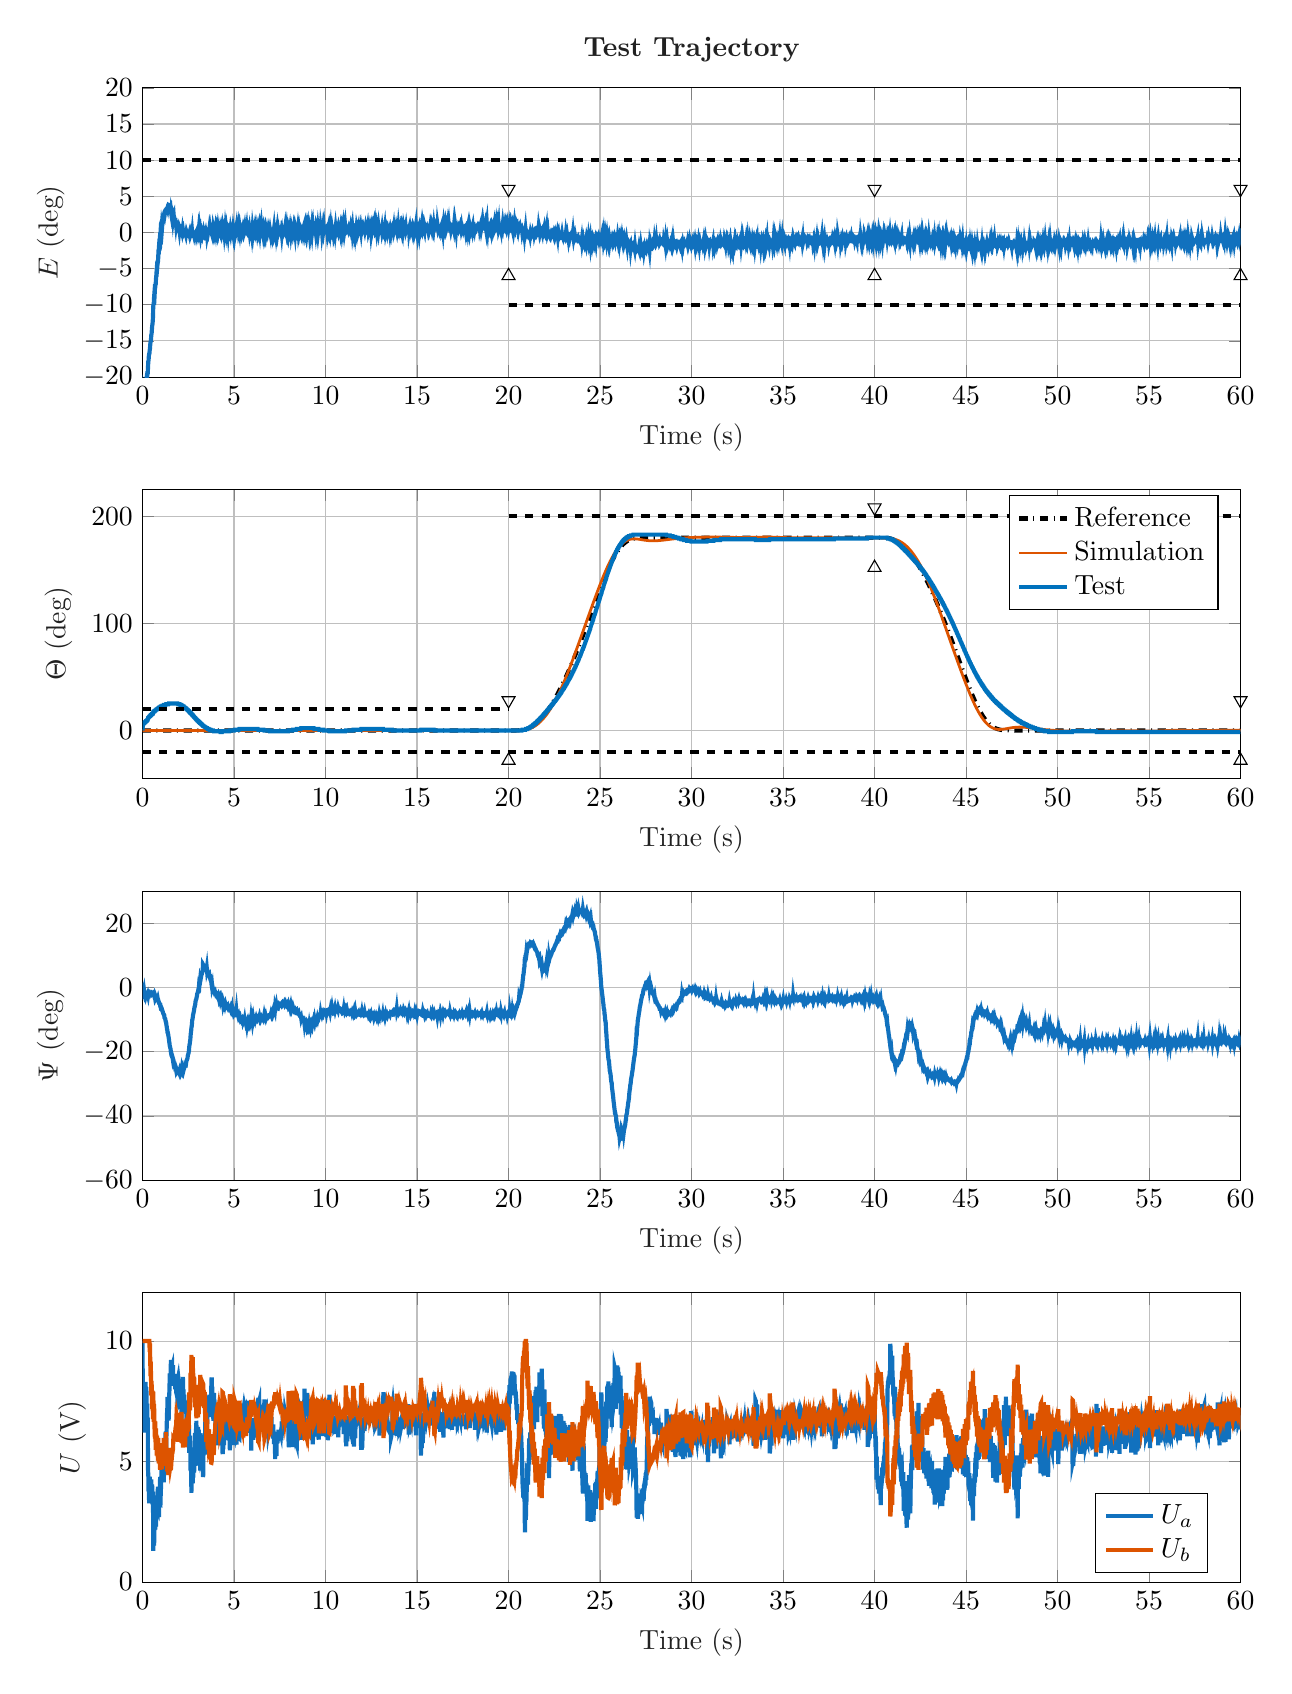
\begin{tikzpicture}

\begin{axis}[%
width=5.49in,
height=1.446in,
at={(0.921in,7.033in)},
scale only axis,
xmin=0,
xmax=60,
xlabel style={font=\color{mycolor2}},
xlabel={Time (s)},
ymin=-20,
ymax=20,
ytick={-20, -15, -10,  -5,   0,   5,  10,  15,  20},
ylabel style={font=\color{mycolor2}},
ylabel={$E$ (deg)},
axis background/.style={fill=white},
title style={font=\bfseries\color{mycolor2}},
title={Test Trajectory},
xmajorgrids,
ymajorgrids
]
\addplot [color=mycolor1, line width=1.5pt, forget plot]
  table[row sep=crcr]{%
0	-22.9391505226172\\
0.015	-22.8679618095975\\
0.03	-22.794035069154\\
0.045	-22.6708238350815\\
0.06	-21.8521536353552\\
0.075	-22.0465535824474\\
0.09	-21.4606157137469\\
0.105	-21.8412015256598\\
0.12	-21.7864409771832\\
0.135	-21.4879959879853\\
0.15	-21.244311547264\\
0.165	-21.5482325913096\\
0.18	-21.4085931926941\\
0.195	-21.1211003131915\\
0.21	-20.8883679821656\\
0.225	-20.4940920331335\\
0.24	-20.1600526874258\\
0.255	-19.8588696708041\\
0.27	-19.5220922976725\\
0.285	-19.4700697766197\\
0.3	-18.5309263702446\\
0.315	-17.8382054320147\\
0.33	-17.6793998414323\\
0.345	-17.0715577533412\\
0.36	-16.8087071206531\\
0.375	-16.7621606544479\\
0.39	-16.3213382392107\\
0.405	-16.0776537984895\\
0.42	-15.5108821217558\\
0.435	-15.1713667212004\\
0.45	-15.0207752128896\\
0.465	-14.6703077026388\\
0.48	-14.1309163001435\\
0.495	-14.0022290112233\\
0.51	-13.4546235264566\\
0.525	-12.9617785901665\\
0.54	-12.7290462591406\\
0.555	-12.359412556923\\
0.57	-11.6940718929314\\
0.585	-10.1717286452797\\
0.6	-9.94994842394916\\
0.615	-9.70078792838027\\
0.63	-8.99711488045495\\
0.645	-8.49605586189335\\
0.66	-8.60557695884671\\
0.675	-7.87452363668305\\
0.69	-7.60072089429966\\
0.705	-7.26120549374425\\
0.72	-7.13799425967172\\
0.735	-6.37956066326973\\
0.75	-6.04004526271433\\
0.765	-5.48696372309988\\
0.78	-4.98590470453827\\
0.795	-5.06256947240562\\
0.81	-4.6326991668637\\
0.825	-4.08235565467308\\
0.84	-4.06592749013007\\
0.855	-3.56486847156847\\
0.87	-2.49703777627325\\
0.885	-2.43132511810123\\
0.9	-1.91109990757279\\
0.915	-1.98776467544014\\
0.93	-1.51682395854071\\
0.945	-0.925410034992584\\
0.96	-0.985646638316932\\
0.975	-0.347686248563629\\
0.99	-0.514705921417497\\
1.005	0.0821840569783034\\
1.02	0.257417812103672\\
1.035	0.388843128447694\\
1.05	0.85704581792329\\
1.065	0.62978954174508\\
1.08	1.11442039576368\\
1.095	1.43840437821907\\
1.11	1.45007027103101\\
1.125	1.49965031548174\\
1.14	1.998367233192\\
1.155	2.29584749989636\\
1.17	2.46208647246645\\
1.185	2.42417232082766\\
1.2	2.30168044630233\\
1.215	2.54083124894702\\
1.23	2.89372450650808\\
1.245	3.07454584509309\\
1.26	3.10371057712293\\
1.275	3.09496115751397\\
1.29	3.22328597844527\\
1.305	3.25536718367809\\
1.32	3.28161544250495\\
1.335	3.25536718367809\\
1.35	3.36036021898552\\
1.365	3.23495187125721\\
1.38	3.50035093272875\\
1.395	3.73950173537343\\
1.41	3.81241356544803\\
1.425	3.78908177982416\\
1.44	3.69867111053166\\
1.455	3.44493794187205\\
1.47	3.40119084382729\\
1.485	3.08329526470204\\
1.5	3.04246463986026\\
1.515	3.30494722812882\\
1.53	3.38369200460939\\
1.545	2.95788691697373\\
1.56	2.72165258753202\\
1.575	3.12120941634083\\
1.59	2.95497044377074\\
1.605	2.58457834699178\\
1.62	2.41250642801572\\
1.635	2.6895713822992\\
1.65	2.54666419535299\\
1.665	2.11794263451434\\
1.68	2.43875468684258\\
1.695	2.53791477574403\\
1.71	1.96628602795917\\
1.725	2.14710736654418\\
1.74	1.98961781358304\\
1.755	1.88754125147861\\
1.77	1.49381736907577\\
1.785	1.96920250116216\\
1.8	1.63672455602198\\
1.815	1.44715379782802\\
1.83	1.08430209410151\\
1.845	1.35674312853552\\
1.86	1.3596596017385\\
1.875	1.18287108135953\\
1.89	0.928234530942977\\
1.905	1.05418379243934\\
1.92	1.17465699908803\\
1.935	1.12537250545902\\
1.95	0.906330311552307\\
1.965	0.818713433989619\\
1.98	0.826927516261119\\
1.995	0.616099404625911\\
2.01	0.345034689666353\\
2.025	0.687288117645591\\
2.04	0.58598110296374\\
2.055	1.13084856030669\\
2.07	0.731096556426938\\
2.085	0.358724826785523\\
2.1	0.232775565289164\\
2.115	0.240989647560664\\
2.13	0.703716282188598\\
2.145	0.202657263626993\\
2.16	0.0383756181969559\\
2.175	0.279322031494335\\
2.19	-0.00543282058438455\\
2.205	-0.0766215336040716\\
2.22	0.0739699747067959\\
2.235	-0.202570795100431\\
2.25	-0.123167999809243\\
2.265	-0.0218609851273925\\
2.28	0.0438516730446181\\
2.295	0.00551928911094701\\
2.31	-0.00817084800822276\\
2.325	0.421699457533703\\
2.34	-0.0163849302797232\\
2.355	-0.188880657981261\\
2.37	-0.33673413886829\\
2.385	-0.0985257529947419\\
2.4	0.117778413488136\\
2.415	4.3234263284786e-05\\
2.43	-0.227213041914932\\
2.445	-0.303877809782281\\
2.46	-0.281973590391611\\
2.475	-0.0245990125512237\\
2.49	0.0109953439586163\\
2.505	-0.208046849948093\\
2.52	-0.298401754934612\\
2.535	-0.369590467954299\\
2.55	-0.150548274047583\\
2.565	-0.0136469028558921\\
2.58	-0.235427124186433\\
2.595	-0.156024328895252\\
2.61	-0.402446797040308\\
2.625	-0.281973590391611\\
2.64	-0.0547173142133943\\
2.655	-0.180666575709753\\
2.67	-0.139596164352251\\
2.685	-0.358638358258961\\
2.7	-0.375066522801969\\
2.715	-0.0547173142133943\\
2.73	-0.459945372940818\\
2.745	-0.47089748263615\\
2.76	-0.0766215336040716\\
2.775	-0.0629313964848948\\
2.79	-0.218998959643432\\
2.805	-0.37232849537813\\
2.82	-0.131382082080751\\
2.835	-0.131382082080751\\
2.85	-0.161500383742921\\
2.865	-0.481849592331488\\
2.88	-0.533872113384329\\
2.895	-0.0574553416372325\\
2.91	0.0109953439586163\\
2.925	-0.312091892053789\\
2.94	-0.525658031112829\\
2.955	-0.369590467954299\\
2.97	-0.394232714768808\\
2.985	-0.183404603133592\\
3	-0.30113978235845\\
3.015	-0.22995106933877\\
3.03	-0.30661583720612\\
3.045	-0.35042427598746\\
3.06	0.0274235085016243\\
3.075	-0.323044001749121\\
3.09	-0.199832767676593\\
3.105	-0.33673413886829\\
3.12	0.123254468335806\\
3.135	-0.197094740252761\\
3.15	-0.19435671282893\\
3.165	-0.438041153550141\\
3.18	-0.172452493438253\\
3.195	-0.473635510059981\\
3.21	-0.317567946901451\\
3.225	-0.30661583720612\\
3.24	-0.424351016430978\\
3.255	-0.199832767676593\\
3.27	-0.361376385682799\\
3.285	-0.405184824464139\\
3.3	0.446341704348204\\
3.315	0.402533265566871\\
3.33	-0.276497535543949\\
3.345	-0.26554542584861\\
3.36	0.0520657553161257\\
3.375	-0.0957877255709036\\
3.39	-0.188880657981261\\
3.405	-0.0410271770942316\\
3.42	0.0684939198591266\\
3.435	-0.281973590391611\\
3.45	-0.281973590391611\\
3.465	-0.0848356158755721\\
3.48	-0.284711617815449\\
3.495	-0.37232849537813\\
3.51	0.0493277278922875\\
3.525	-0.35042427598746\\
3.54	-0.131382082080751\\
3.555	-0.0547173142133943\\
3.57	-0.169714466014422\\
3.585	0.0630178650114572\\
3.6	0.0109953439586163\\
3.615	-0.00543282058438455\\
3.63	0.0356375907731177\\
3.645	0.334082579971015\\
3.66	0.0548037827399639\\
3.675	0.093136166673635\\
3.69	0.380629046176193\\
3.705	0.0903981392497968\\
3.72	0.093136166673635\\
3.735	0.169800934540984\\
3.75	0.577767020692239\\
3.765	0.00551928911094701\\
3.78	-0.125906027233081\\
3.795	0.460031841467381\\
3.81	-0.030075067398893\\
3.825	0.361462854209354\\
3.84	0.331344552547183\\
3.855	0.158848824845646\\
3.87	0.62157545947358\\
3.885	0.443603676924373\\
3.9	0.232775565289164\\
3.915	0.194443181355486\\
3.93	0.0630178650114572\\
3.945	0.410747347838371\\
3.96	-0.00817084800822276\\
3.975	0.147896715150314\\
3.99	0.429913539805203\\
4.005	0.161586852269477\\
4.02	0.470983951162712\\
4.035	0.457293814043543\\
4.05	0.254679784679834\\
4.065	0.0712319472829577\\
4.08	0.470983951162712\\
4.095	0.306702305732675\\
4.11	0.147896715150314\\
4.125	0.48741211570572\\
4.14	0.221823455593825\\
4.155	0.202657263626993\\
4.17	0.312178360580344\\
4.185	-0.0629313964848948\\
4.2	0.481936060858044\\
4.215	0.0137333713824475\\
4.23	-0.0875736432994032\\
4.245	0.421699457533703\\
4.26	-0.0245990125512237\\
4.275	0.386105101023863\\
4.29	0.219085428169994\\
4.305	0.147896715150314\\
4.32	0.383367073600031\\
4.335	0.136944605454975\\
4.35	0.347772717090191\\
4.365	0.339558634818684\\
4.38	0.449079731772042\\
4.395	-0.139596164352251\\
4.41	0.49288817055339\\
4.425	0.303964278308844\\
4.44	0.232775565289164\\
4.455	0.418961430109864\\
4.47	0.0383756181969559\\
4.485	0.377891018752362\\
4.5	0.394319183295363\\
4.515	4.3234263284786e-05\\
4.53	0.470983951162712\\
4.545	0.180753044236316\\
4.56	0.0821840569783034\\
4.575	0.355986799361692\\
4.59	0.021947453653955\\
4.605	0.262893866951335\\
4.62	0.249203729832165\\
4.635	0.186229099083985\\
4.65	0.271107949222835\\
4.665	-0.0355511222465623\\
4.68	0.418961430109864\\
4.695	0.312178360580344\\
4.71	0.309440333156513\\
4.725	0.429913539805203\\
4.74	0.402533265566871\\
4.755	0.205395291050824\\
4.77	0.383367073600031\\
4.785	0.232775565289164\\
4.8	0.0356375907731177\\
4.815	0.375152991328531\\
4.83	0.164324879693315\\
4.845	0.284798086342005\\
4.86	0.164324879693315\\
4.875	0.109564331216636\\
4.89	0.755738803241439\\
4.905	0.076708002130627\\
4.92	0.180753044236316\\
4.935	0.372414963904693\\
4.95	0.101350248945135\\
4.965	0.503840280248721\\
4.98	0.293012168613512\\
4.995	0.0192094262301168\\
5.01	0.52300647221556\\
5.025	0.408009320414533\\
5.04	0.0027812616871159\\
5.055	0.314916388004183\\
5.07	0.254679784679834\\
5.085	0.0657558924352954\\
5.1	0.268369921799004\\
5.115	0.375152991328531\\
5.13	0.62978954174508\\
5.145	0.235513592712995\\
5.16	0.361462854209354\\
5.175	0.394319183295363\\
5.19	0.131468550607306\\
5.205	0.205395291050824\\
5.22	0.457293814043543\\
5.235	-0.0382891496703934\\
5.25	0.490150143129551\\
5.265	0.0465897004684563\\
5.28	0.188967126507816\\
5.295	0.372414963904693\\
5.31	0.117778413488136\\
5.325	0.460031841467381\\
5.34	0.205395291050824\\
5.355	0.380629046176193\\
5.37	0.306702305732675\\
5.385	0.131468550607306\\
5.4	0.457293814043543\\
5.415	0.5503867464539\\
5.43	-0.0437652045180628\\
5.445	0.542172664182392\\
5.46	0.208133318474655\\
5.475	0.361462854209354\\
5.49	0.553124773877731\\
5.505	0.358724826785523\\
5.52	0.131468550607306\\
5.535	0.314916388004183\\
5.55	0.106826303792805\\
5.565	0.262893866951335\\
5.58	0.501102252824883\\
5.595	0.145158687726476\\
5.61	0.249203729832165\\
5.625	0.435389594652872\\
5.64	0.358724826785523\\
5.655	0.175276989388654\\
5.67	0.115040386064305\\
5.685	0.388843128447694\\
5.7	-0.0766215336040716\\
5.715	0.501102252824883\\
5.73	0.416223402686033\\
5.745	0.251941757256003\\
5.76	0.147896715150314\\
5.775	0.101350248945135\\
5.79	0.298488223461175\\
5.805	0.117778413488136\\
5.82	0.199919236203155\\
5.835	0.429913539805203\\
5.85	0.109564331216636\\
5.865	0.347772717090191\\
5.88	0.131468550607306\\
5.895	0.180753044236316\\
5.91	0.210871345898494\\
5.925	0.142420660302645\\
5.94	0.67907403537409\\
5.955	0.271107949222835\\
5.97	-0.0437652045180628\\
5.985	0.416223402686033\\
6	-0.120429972385412\\
6.015	0.397057210719194\\
6.03	0.109564331216636\\
6.045	0.454555786619704\\
6.06	0.0328995633492866\\
6.075	0.112302358640474\\
6.09	0.290274141189674\\
6.105	0.156110797421815\\
6.12	0.380629046176193\\
6.135	-0.0328130948227241\\
6.15	0.345034689666353\\
6.165	0.520268444791722\\
6.18	0.0493277278922875\\
6.195	0.451817759195873\\
6.21	0.0301615359254555\\
6.225	0.150634742574145\\
6.24	0.323130470275683\\
6.255	0.309440333156513\\
6.27	0.481936060858044\\
6.285	0.134206578031137\\
6.3	0.361462854209354\\
6.315	0.460031841467381\\
6.33	0.224561483017663\\
6.345	0.427175512381372\\
6.36	-0.0136469028558921\\
6.375	0.0520657553161257\\
6.39	0.386105101023863\\
6.405	0.101350248945135\\
6.42	0.498364225401052\\
6.435	0.273845976646673\\
6.45	0.531220554487061\\
6.465	0.238251620136833\\
6.48	0.235513592712995\\
6.495	0.591457157811402\\
6.51	0.194443181355486\\
6.525	0.306702305732675\\
6.54	0.169800934540984\\
6.555	0.254679784679834\\
6.57	0.331344552547183\\
6.585	0.0520657553161257\\
6.6	0.298488223461175\\
6.615	0.0164713988062857\\
6.63	0.380629046176193\\
6.645	0.421699457533703\\
6.66	0.235513592712995\\
6.675	0.306702305732675\\
6.69	0.0109953439586163\\
6.705	0.284798086342005\\
6.72	0.0438516730446181\\
6.735	0.402533265566871\\
6.75	-0.0574553416372325\\
6.765	0.262893866951335\\
6.78	0.076708002130627\\
6.795	0.254679784679834\\
6.81	0.164324879693315\\
6.825	0.00825731653477813\\
6.84	0.216347400746156\\
6.855	0.158848824845646\\
6.87	0.399795238143032\\
6.885	0.202657263626993\\
6.9	0.0356375907731177\\
6.915	0.076708002130627\\
6.93	0.167062907117153\\
6.945	0.183491071660154\\
6.96	0.388843128447694\\
6.975	0.153372769997976\\
6.99	0.690026145069422\\
7.005	0.306702305732675\\
7.02	0.131468550607306\\
7.035	0.503840280248721\\
7.05	-0.0820975884517339\\
7.065	0.46550789631505\\
7.08	-0.0574553416372325\\
7.095	0.451817759195873\\
7.11	0.0356375907731177\\
7.125	0.462769868891212\\
7.14	-0.0109088754320539\\
7.155	0.197181208779324\\
7.17	0.158848824845646\\
7.185	0.462769868891212\\
7.2	0.0548037827399639\\
7.215	0.230037537865333\\
7.23	0.0328995633492866\\
7.245	0.774904995208271\\
7.26	0.399795238143032\\
7.275	0.00551928911094701\\
7.29	0.369676936480855\\
7.305	0.366938909057023\\
7.32	0.690026145069422\\
7.335	0.0903981392497968\\
7.35	0.358724826785523\\
7.365	0.104088276368967\\
7.38	0.432651567229041\\
7.395	0.128730523183475\\
7.41	0.279322031494335\\
7.425	4.3234263284786e-05\\
7.44	0.136944605454975\\
7.455	0.232775565289164\\
7.47	0.284798086342005\\
7.485	0.169800934540984\\
7.5	0.158848824845646\\
7.515	0.227299510441495\\
7.53	0.301226250885013\\
7.545	0.268369921799004\\
7.56	0.394319183295363\\
7.575	0.169800934540984\\
7.59	0.323130470275683\\
7.605	-0.0273370399750548\\
7.62	0.366938909057023\\
7.635	0.257417812103672\\
7.65	0.323130470275683\\
7.665	-0.0766215336040716\\
7.68	0.0438516730446181\\
7.695	0.320392442851852\\
7.71	0.331344552547183\\
7.725	0.00825731653477813\\
7.74	0.101350248945135\\
7.755	0.273845976646673\\
7.77	0.180753044236316\\
7.785	0.457293814043543\\
7.8	0.0383756181969559\\
7.815	0.0192094262301168\\
7.83	0.131468550607306\\
7.845	0.443603676924373\\
7.86	0.219085428169994\\
7.875	0.514792389944053\\
7.89	0.156110797421815\\
7.905	-0.0793595610279028\\
7.92	0.169800934540984\\
7.935	0.240989647560664\\
7.95	0.0164713988062857\\
7.965	0.446341704348204\\
7.98	0.0383756181969559\\
7.995	0.427175512381372\\
8.01	0.276584004070504\\
8.025	0.306702305732675\\
8.04	0.136944605454975\\
8.055	0.402533265566871\\
8.07	0.0739699747067959\\
8.085	0.531220554487061\\
8.1	0.0821840569783034\\
8.115	0.813237379141957\\
8.13	0.246465702408334\\
8.145	0.517530417367891\\
8.16	0.331344552547183\\
8.175	0.418961430109864\\
8.19	0.377891018752362\\
8.205	-0.030075067398893\\
8.22	-0.0109088754320539\\
8.235	0.531220554487061\\
8.25	0.0903981392497968\\
8.265	0.254679784679834\\
8.28	0.59419518523524\\
8.295	0.391581155871525\\
8.31	0.271107949222835\\
8.325	0.345034689666353\\
8.34	0.0246854810777861\\
8.355	0.454555786619704\\
8.37	0.262893866951335\\
8.385	0.306702305732675\\
8.4	0.355986799361692\\
8.415	0.339558634818684\\
8.43	0.413485375262202\\
8.445	0.178015016812485\\
8.46	0.0109953439586163\\
8.475	0.188967126507816\\
8.49	0.495626197977221\\
8.505	0.169800934540984\\
8.52	0.780381050055948\\
8.535	0.191705153931655\\
8.55	0.421699457533703\\
8.565	0.136944605454975\\
8.58	0.355986799361692\\
8.595	0.178015016812485\\
8.61	0.188967126507816\\
8.625	0.243727674984495\\
8.64	0.0903981392497968\\
8.655	0.506578307672552\\
8.67	-0.0601933690610637\\
8.685	0.473721978586543\\
8.7	0.397057210719194\\
8.715	0.331344552547183\\
8.73	0.216347400746156\\
8.745	0.298488223461175\\
8.76	0.0684939198591266\\
8.775	0.350510744514023\\
8.79	0.624313486897411\\
8.805	0.755738803241439\\
8.82	0.254679784679834\\
8.835	0.440865649500542\\
8.85	0.0246854810777861\\
8.865	0.383367073600031\\
8.88	0.60788532235441\\
8.895	0.194443181355486\\
8.91	0.405271292990702\\
8.925	0.49288817055339\\
8.94	0.536696609334723\\
8.955	0.213609373322325\\
8.97	0.490150143129551\\
8.985	0.147896715150314\\
9	0.446341704348204\\
9.015	0.317654415428014\\
9.03	0.57229096584457\\
9.045	0.117778413488136\\
9.06	0.5503867464539\\
9.075	0.394319183295363\\
9.09	0.293012168613512\\
9.105	0.490150143129551\\
9.12	0.131468550607306\\
9.135	0.490150143129551\\
9.15	0.62157545947358\\
9.165	0.503840280248721\\
9.18	0.0876601118259657\\
9.195	0.372414963904693\\
9.21	0.410747347838371\\
9.225	0.273845976646673\\
9.24	0.542172664182392\\
9.255	0.221823455593825\\
9.27	0.662645870831089\\
9.285	0.388843128447694\\
9.3	0.673597980526421\\
9.315	0.232775565289164\\
9.33	0.293012168613512\\
9.345	0.202657263626993\\
9.36	0.199919236203155\\
9.375	0.580505048116071\\
9.39	0.156110797421815\\
9.405	0.596933212659071\\
9.42	0.021947453653955\\
9.435	0.306702305732675\\
9.45	0.476460006010382\\
9.465	0.153372769997976\\
9.48	0.512054362520222\\
9.495	0.317654415428014\\
9.51	0.484674088281882\\
9.525	0.0876601118259657\\
9.54	0.249203729832165\\
9.555	0.462769868891212\\
9.57	0.142420660302645\\
9.585	0.514792389944053\\
9.6	0.202657263626993\\
9.615	0.509316335096383\\
9.63	0.588719130387571\\
9.645	0.399795238143032\\
9.66	0.476460006010382\\
9.675	0.295750196037343\\
9.69	0.339558634818684\\
9.705	0.262893866951335\\
9.72	0.230037537865333\\
9.735	0.71466839188393\\
9.75	0.440865649500542\\
9.765	0.350510744514023\\
9.78	0.525744499639391\\
9.795	0.57229096584457\\
9.81	0.0903981392497968\\
9.825	0.377891018752362\\
9.84	0.457293814043543\\
9.855	0.276584004070504\\
9.87	0.610623349778241\\
9.885	0.345034689666353\\
9.9	0.638003624016581\\
9.915	0.158848824845646\\
9.93	0.276584004070504\\
9.945	0.227299510441495\\
9.96	0.243727674984495\\
9.975	0.205395291050824\\
9.99	0.481936060858044\\
10.005	0.399795238143032\\
10.02	0.468245923738881\\
10.035	0.150634742574145\\
10.05	0.939186640638309\\
10.065	0.583243075539902\\
10.08	0.544910691606231\\
10.095	0.169800934540984\\
10.11	0.451817759195873\\
10.125	0.840617653380289\\
10.14	0.446341704348204\\
10.155	0.624313486897411\\
10.17	0.150634742574145\\
10.185	0.320392442851852\\
10.2	0.369676936480855\\
10.215	0.136944605454975\\
10.23	0.350510744514023\\
10.245	0.577767020692239\\
10.26	0.265631894375173\\
10.275	0.577767020692239\\
10.29	0.158848824845646\\
10.305	0.533958581910892\\
10.32	0.462769868891212\\
10.335	0.306702305732675\\
10.35	0.52300647221556\\
10.365	0.268369921799004\\
10.38	0.262893866951335\\
10.395	0.290274141189674\\
10.41	0.101350248945135\\
10.425	0.509316335096383\\
10.44	0.115040386064305\\
10.455	0.350510744514023\\
10.47	0.457293814043543\\
10.485	0.405271292990702\\
10.5	0.408009320414533\\
10.515	0.473721978586543\\
10.53	0.139682632878814\\
10.545	0.473721978586543\\
10.56	0.117778413488136\\
10.575	0.312178360580344\\
10.59	0.350510744514023\\
10.605	0.257417812103672\\
10.62	0.418961430109864\\
10.635	0.451817759195873\\
10.65	0.451817759195873\\
10.665	0.599671240082903\\
10.68	0.208133318474655\\
10.695	0.906330311552307\\
10.71	0.399795238143032\\
10.725	0.167062907117153\\
10.74	0.320392442851852\\
10.755	0.276584004070504\\
10.77	0.279322031494335\\
10.785	0.355986799361692\\
10.8	0.251941757256003\\
10.815	0.49288817055339\\
10.83	0.186229099083985\\
10.845	0.429913539805203\\
10.86	0.62157545947358\\
10.875	0.197181208779324\\
10.89	0.591457157811402\\
10.905	0.63526559659275\\
10.92	0.147896715150314\\
10.935	0.383367073600031\\
10.95	0.375152991328531\\
10.965	0.191705153931655\\
10.98	0.46550789631505\\
10.995	0.807761324294287\\
11.01	0.503840280248721\\
11.025	0.158848824845646\\
11.04	0.418961430109864\\
11.055	0.840617653380289\\
11.07	0.235513592712995\\
11.085	0.583243075539902\\
11.1	0.186229099083985\\
11.115	0.240989647560664\\
11.13	0.62978954174508\\
11.145	0.167062907117153\\
11.16	0.221823455593825\\
11.175	0.67085995310259\\
11.19	0.0602798375876261\\
11.205	0.366938909057023\\
11.22	0.314916388004183\\
11.235	0.227299510441495\\
11.25	0.369676936480855\\
11.265	0.153372769997976\\
11.28	0.125992495759637\\
11.295	0.627051514321242\\
11.31	0.605147294930572\\
11.325	0.268369921799004\\
11.34	0.345034689666353\\
11.355	0.298488223461175\\
11.37	0.240989647560664\\
11.385	0.531220554487061\\
11.4	0.317654415428014\\
11.415	0.48741211570572\\
11.43	0.651693761135751\\
11.445	0.402533265566871\\
11.46	0.651693761135751\\
11.475	0.199919236203155\\
11.49	0.49288817055339\\
11.505	0.268369921799004\\
11.52	0.213609373322325\\
11.535	0.484674088281882\\
11.55	0.490150143129551\\
11.565	0.295750196037343\\
11.58	0.638003624016581\\
11.595	0.112302358640474\\
11.61	0.325868497699514\\
11.625	0.65716981598342\\
11.64	0.186229099083985\\
11.655	0.501102252824883\\
11.67	0.440865649500542\\
11.685	0.235513592712995\\
11.7	0.638003624016581\\
11.715	0.446341704348204\\
11.73	0.339558634818684\\
11.745	0.416223402686033\\
11.76	0.564076883573063\\
11.775	0.369676936480855\\
11.79	0.553124773877731\\
11.805	0.169800934540984\\
11.82	0.295750196037343\\
11.835	0.240989647560664\\
11.85	0.257417812103672\\
11.865	0.199919236203155\\
11.88	0.219085428169994\\
11.895	0.320392442851852\\
11.91	0.364200881633185\\
11.925	0.59419518523524\\
11.94	0.309440333156513\\
11.955	0.684550090221759\\
11.97	0.520268444791722\\
11.985	0.418961430109864\\
12	0.566814910996901\\
12.015	0.361462854209354\\
12.03	0.48741211570572\\
12.045	0.197181208779324\\
12.06	0.249203729832165\\
12.075	0.358724826785523\\
12.09	0.339558634818684\\
12.105	0.328606525123352\\
12.12	0.402533265566871\\
12.135	0.514792389944053\\
12.15	0.314916388004183\\
12.165	0.520268444791722\\
12.18	0.197181208779324\\
12.195	0.213609373322325\\
12.21	0.484674088281882\\
12.225	0.60788532235441\\
12.24	0.402533265566871\\
12.255	0.476460006010382\\
12.27	0.575028993268401\\
12.285	0.495626197977221\\
12.3	0.71466839188393\\
12.315	0.350510744514023\\
12.33	0.394319183295363\\
12.345	0.709192337036261\\
12.36	0.186229099083985\\
12.375	0.323130470275683\\
12.39	0.345034689666353\\
12.405	0.446341704348204\\
12.42	0.301226250885013\\
12.435	0.575028993268401\\
12.45	0.361462854209354\\
12.465	0.293012168613512\\
12.48	0.473721978586543\\
12.495	0.0164713988062857\\
12.51	0.298488223461175\\
12.525	0.309440333156513\\
12.54	0.564076883573063\\
12.555	0.320392442851852\\
12.57	0.509316335096383\\
12.585	0.191705153931655\\
12.6	0.238251620136833\\
12.615	0.249203729832165\\
12.63	0.501102252824883\\
12.645	0.00825731653477813\\
12.66	0.355986799361692\\
12.675	0.410747347838371\\
12.69	0.216347400746156\\
12.705	0.186229099083985\\
12.72	0.575028993268401\\
12.735	0.219085428169994\\
12.75	0.301226250885013\\
12.765	0.432651567229041\\
12.78	0.684550090221759\\
12.795	0.364200881633185\\
12.81	0.681812062797921\\
12.825	0.528482527063223\\
12.84	0.366938909057023\\
12.855	0.533958581910892\\
12.87	0.542172664182392\\
12.885	0.298488223461175\\
12.9	0.632527569168911\\
12.915	0.320392442851852\\
12.93	0.350510744514023\\
12.945	0.851569763075628\\
12.96	0.408009320414533\\
12.975	0.276584004070504\\
12.99	0.358724826785523\\
13.005	0.528482527063223\\
13.02	0.476460006010382\\
13.035	0.460031841467381\\
13.05	0.314916388004183\\
13.065	0.235513592712995\\
13.08	0.476460006010382\\
13.095	0.136944605454975\\
13.11	0.312178360580344\\
13.125	0.651693761135751\\
13.14	0.197181208779324\\
13.155	0.0876601118259657\\
13.17	0.375152991328531\\
13.185	0.421699457533703\\
13.2	0.180753044236316\\
13.215	0.284798086342005\\
13.23	0.542172664182392\\
13.245	0.0137333713824475\\
13.26	0.438127622076711\\
13.275	0.753000775817608\\
13.29	0.249203729832165\\
13.305	0.451817759195873\\
13.32	0.577767020692239\\
13.335	0.353248771937854\\
13.35	0.410747347838371\\
13.365	0.512054362520222\\
13.38	0.251941757256003\\
13.395	0.484674088281882\\
13.41	0.506578307672552\\
13.425	0.394319183295363\\
13.44	0.432651567229041\\
13.455	0.49288817055339\\
13.47	0.339558634818684\\
13.485	0.336820607394853\\
13.5	0.468245923738881\\
13.515	0.161586852269477\\
13.53	0.46550789631505\\
13.545	0.408009320414533\\
13.56	0.210871345898494\\
13.575	0.569552938420732\\
13.59	0.64347967886425\\
13.605	0.230037537865333\\
13.62	0.284798086342005\\
13.635	0.583243075539902\\
13.65	0.66538389825492\\
13.665	0.536696609334723\\
13.68	0.5503867464539\\
13.695	0.424437484957534\\
13.71	0.295750196037343\\
13.725	0.555862801301562\\
13.74	0.164324879693315\\
13.755	0.309440333156513\\
13.77	0.355986799361692\\
13.785	0.654431788559582\\
13.8	0.547648719030062\\
13.815	0.481936060858044\\
13.83	0.172538961964815\\
13.845	0.175276989388654\\
13.86	0.284798086342005\\
13.875	0.58598110296374\\
13.89	0.394319183295363\\
13.905	0.197181208779324\\
13.92	0.438127622076711\\
13.935	0.429913539805203\\
13.95	0.282060058918174\\
13.965	0.180753044236316\\
13.98	0.583243075539902\\
13.995	0.230037537865333\\
14.01	0.158848824845646\\
14.025	0.64347967886425\\
14.04	0.64347967886425\\
14.055	0.591457157811402\\
14.07	0.553124773877731\\
14.085	0.703716282188598\\
14.1	0.287536113765843\\
14.115	0.323130470275683\\
14.13	0.62978954174508\\
14.145	0.460031841467381\\
14.16	0.265631894375173\\
14.175	0.57229096584457\\
14.19	0.495626197977221\\
14.205	0.276584004070504\\
14.22	0.7283585290031\\
14.235	0.599671240082903\\
14.25	0.262893866951335\\
14.265	0.268369921799004\\
14.28	0.720144446731599\\
14.295	0.542172664182392\\
14.31	0.429913539805203\\
14.325	0.566814910996901\\
14.34	0.651693761135751\\
14.355	0.369676936480855\\
14.37	0.408009320414533\\
14.385	0.63526559659275\\
14.4	0.265631894375173\\
14.415	0.394319183295363\\
14.43	0.509316335096383\\
14.445	0.476460006010382\\
14.46	0.0739699747067959\\
14.475	0.57229096584457\\
14.49	0.536696609334723\\
14.505	0.364200881633185\\
14.52	4.3234263284786e-05\\
14.535	0.610623349778241\\
14.55	1.01311338108183\\
14.565	0.383367073600031\\
14.58	0.63526559659275\\
14.595	0.791333159751279\\
14.61	0.514792389944053\\
14.625	0.476460006010382\\
14.64	0.698240227340929\\
14.655	0.613361377202079\\
14.67	0.388843128447694\\
14.685	0.555862801301562\\
14.7	0.640741651440419\\
14.715	0.481936060858044\\
14.73	0.501102252824883\\
14.745	0.67085995310259\\
14.76	0.501102252824883\\
14.775	0.240989647560664\\
14.79	0.446341704348204\\
14.805	0.739310638698438\\
14.82	0.62978954174508\\
14.835	0.394319183295363\\
14.85	0.416223402686033\\
14.865	0.785857104903617\\
14.88	0.158848824845646\\
14.895	0.317654415428014\\
14.91	0.334082579971015\\
14.925	0.668121925678758\\
14.94	0.936448613214478\\
14.955	0.481936060858044\\
14.97	0.575028993268401\\
14.985	0.399795238143032\\
15	0.131468550607306\\
15.015	0.62978954174508\\
15.03	0.561338856149231\\
15.045	0.481936060858044\\
15.06	0.224561483017663\\
15.075	0.394319183295363\\
15.09	0.520268444791722\\
15.105	0.659907843407251\\
15.12	0.306702305732675\\
15.135	0.684550090221759\\
15.15	0.624313486897411\\
15.165	0.342296662242522\\
15.18	0.410747347838371\\
15.195	0.791333159751279\\
15.21	0.695502199917098\\
15.225	0.380629046176193\\
15.24	0.514792389944053\\
15.255	0.79954724202278\\
15.27	0.383367073600031\\
15.285	0.235513592712995\\
15.3	0.408009320414533\\
15.315	0.818713433989619\\
15.33	0.57229096584457\\
15.345	0.388843128447694\\
15.36	0.457293814043543\\
15.375	0.71466839188393\\
15.39	0.49288817055339\\
15.405	0.328606525123352\\
15.42	0.747524720969939\\
15.435	0.583243075539902\\
15.45	0.564076883573063\\
15.465	0.553124773877731\\
15.48	0.632527569168911\\
15.495	0.695502199917098\\
15.51	0.287536113765843\\
15.525	0.651693761135751\\
15.54	1.08977814894918\\
15.555	0.70097825476476\\
15.57	0.525744499639391\\
15.585	0.48741211570572\\
15.6	0.555862801301562\\
15.615	0.328606525123352\\
15.63	0.49288817055339\\
15.645	0.539434636758561\\
15.66	0.651693761135751\\
15.675	0.377891018752362\\
15.69	0.528482527063223\\
15.705	0.481936060858044\\
15.72	0.753000775817608\\
15.735	0.509316335096383\\
15.75	0.528482527063223\\
15.765	0.71466839188393\\
15.78	0.733834583850769\\
15.795	0.569552938420732\\
15.81	0.917282421247638\\
15.825	0.758476830665278\\
15.84	0.498364225401052\\
15.855	0.662645870831089\\
15.87	1.19108516363103\\
15.885	0.627051514321242\\
15.9	0.438127622076711\\
15.915	0.788595132327448\\
15.93	0.468245923738881\\
15.945	0.624313486897411\\
15.96	0.974780997148149\\
15.975	0.832403571108789\\
15.99	0.520268444791722\\
16.005	0.498364225401052\\
16.02	0.7365726112746\\
16.035	0.613361377202079\\
16.05	0.605147294930572\\
16.065	0.62978954174508\\
16.08	0.958352832605155\\
16.095	0.991209161691157\\
16.11	0.271107949222835\\
16.125	0.92002044867147\\
16.14	0.65716981598342\\
16.155	0.810499351718118\\
16.17	0.70645430961243\\
16.185	0.659907843407251\\
16.2	0.59419518523524\\
16.215	0.429913539805203\\
16.23	0.62157545947358\\
16.245	0.67907403537409\\
16.26	0.703716282188598\\
16.275	0.383367073600031\\
16.29	0.454555786619704\\
16.305	0.687288117645591\\
16.32	0.805023296870449\\
16.335	0.429913539805203\\
16.35	0.577767020692239\\
16.365	0.818713433989619\\
16.38	0.77216696778444\\
16.395	0.553124773877731\\
16.41	0.265631894375173\\
16.425	0.755738803241439\\
16.44	1.04596971016784\\
16.455	0.703716282188598\\
16.47	0.65716981598342\\
16.485	0.85704581792329\\
16.5	0.77216696778444\\
16.515	0.323130470275683\\
16.53	0.462769868891212\\
16.545	0.58598110296374\\
16.56	0.92002044867147\\
16.575	0.668121925678758\\
16.59	0.399795238143032\\
16.605	0.542172664182392\\
16.62	0.963828887452817\\
16.635	0.802285269446611\\
16.65	0.605147294930572\\
16.665	0.676336007950259\\
16.68	0.977519024571987\\
16.695	0.662645870831089\\
16.71	0.602409267506741\\
16.725	0.569552938420732\\
16.74	0.900854256704638\\
16.755	0.520268444791722\\
16.77	0.533958581910892\\
16.785	0.476460006010382\\
16.8	1.11168236833985\\
16.815	0.583243075539902\\
16.83	0.618837432049742\\
16.845	0.402533265566871\\
16.86	0.613361377202079\\
16.875	0.832403571108789\\
16.89	0.774904995208271\\
16.905	1.3246619233027\\
16.92	1.02406549077717\\
16.935	0.65716981598342\\
16.95	0.555862801301562\\
16.965	0.744786693546101\\
16.98	0.876212009890136\\
16.995	0.876212009890136\\
17.01	0.65716981598342\\
17.025	1.0350176004725\\
17.04	0.711930364460099\\
17.055	0.536696609334723\\
17.07	0.506578307672552\\
17.085	1.05144576501551\\
17.1	0.788595132327448\\
17.115	0.70097825476476\\
17.13	0.413485375262202\\
17.145	0.925496503519139\\
17.16	0.846093708227958\\
17.175	0.876212009890136\\
17.19	0.498364225401052\\
17.205	0.427175512381372\\
17.22	0.848831735651797\\
17.235	0.85704581792329\\
17.25	0.569552938420732\\
17.265	0.648955733711919\\
17.28	0.870735955042467\\
17.295	0.79954724202278\\
17.31	0.542172664182392\\
17.325	0.46550789631505\\
17.34	0.76395288551294\\
17.355	0.900854256704638\\
17.37	0.711930364460099\\
17.385	0.618837432049742\\
17.4	0.564076883573063\\
17.415	0.766690912936778\\
17.43	0.449079731772042\\
17.445	0.599671240082903\\
17.46	0.575028993268401\\
17.475	0.774904995208271\\
17.49	0.659907843407251\\
17.505	0.646217706288081\\
17.52	0.481936060858044\\
17.535	0.65716981598342\\
17.55	0.673597980526421\\
17.565	0.687288117645591\\
17.58	0.610623349778241\\
17.595	0.66538389825492\\
17.61	0.769428940360609\\
17.625	0.77216696778444\\
17.64	0.525744499639391\\
17.655	0.944662695485978\\
17.67	0.972042969724318\\
17.685	0.761214858089109\\
17.7	0.758476830665278\\
17.715	0.870735955042467\\
17.73	0.802285269446611\\
17.745	0.473721978586543\\
17.76	0.66538389825492\\
17.775	0.77216696778444\\
17.79	0.952876777757478\\
17.805	0.462769868891212\\
17.82	0.70645430961243\\
17.835	0.676336007950259\\
17.85	0.796809214598949\\
17.865	0.498364225401052\\
17.88	0.837879625956458\\
17.895	0.63526559659275\\
17.91	0.785857104903617\\
17.925	0.681812062797921\\
17.94	0.512054362520222\\
17.955	0.731096556426938\\
17.97	0.774904995208271\\
17.985	0.618837432049742\\
18	0.46550789631505\\
18.015	0.7365726112746\\
18.03	0.70097825476476\\
18.045	0.870735955042467\\
18.06	0.520268444791722\\
18.075	0.731096556426938\\
18.09	0.681812062797921\\
18.105	0.63526559659275\\
18.12	0.70097825476476\\
18.135	0.498364225401052\\
18.15	0.77764302263211\\
18.165	1.09525420379685\\
18.18	0.580505048116071\\
18.195	0.531220554487061\\
18.21	0.843355680804127\\
18.225	0.854307790499459\\
18.24	0.528482527063223\\
18.255	0.616099404625911\\
18.27	0.840617653380289\\
18.285	0.898116229280806\\
18.3	0.791333159751279\\
18.315	0.577767020692239\\
18.33	0.539434636758561\\
18.345	0.862521872770959\\
18.36	0.851569763075628\\
18.375	0.588719130387571\\
18.39	0.5503867464539\\
18.405	0.974780997148149\\
18.42	0.936448613214478\\
18.435	0.528482527063223\\
18.45	0.69276417249326\\
18.465	0.909068338976138\\
18.48	1.05965984728701\\
18.495	0.892640174433137\\
18.51	0.58598110296374\\
18.525	0.802285269446611\\
18.54	1.043231682744\\
18.555	0.528482527063223\\
18.57	0.539434636758561\\
18.585	0.794071187175118\\
18.6	1.09525420379685\\
18.615	0.785857104903617\\
18.63	0.74204866612227\\
18.645	0.876212009890136\\
18.66	1.05965984728701\\
18.675	1.04596971016784\\
18.69	0.65716981598342\\
18.705	0.59419518523524\\
18.72	0.788595132327448\\
18.735	1.0185894359295\\
18.75	0.761214858089109\\
18.765	0.528482527063223\\
18.78	1.04049365532017\\
18.795	1.02132746335333\\
18.81	1.28091482525794\\
18.825	0.684550090221759\\
18.84	0.418961430109864\\
18.855	0.941924668062147\\
18.87	0.917282421247638\\
18.885	0.952876777757478\\
18.9	0.709192337036261\\
18.915	0.739310638698438\\
18.93	0.791333159751279\\
18.945	0.783119077479779\\
18.96	0.769428940360609\\
18.975	0.544910691606231\\
18.99	0.681812062797921\\
19.005	0.512054362520222\\
19.02	0.77764302263211\\
19.035	0.947400722909809\\
19.05	0.832403571108789\\
19.065	0.5503867464539\\
19.08	0.870735955042467\\
19.095	1.05418379243934\\
19.11	0.939186640638309\\
19.125	0.881688064737798\\
19.14	0.520268444791722\\
19.155	0.972042969724318\\
19.17	0.627051514321242\\
19.185	0.813237379141957\\
19.2	0.569552938420732\\
19.215	0.618837432049742\\
19.23	0.903592284128476\\
19.245	0.605147294930572\\
19.26	1.1965612184787\\
19.275	0.591457157811402\\
19.29	0.684550090221759\\
19.305	0.854307790499459\\
19.32	0.79954724202278\\
19.335	1.12263447803519\\
19.35	0.83514159853262\\
19.365	0.791333159751279\\
19.38	0.881688064737798\\
19.395	0.720144446731599\\
19.41	1.026803518201\\
19.425	0.791333159751279\\
19.44	0.769428940360609\\
19.455	1.05144576501551\\
19.47	0.503840280248721\\
19.485	0.638003624016581\\
19.5	0.60788532235441\\
19.515	0.846093708227958\\
19.53	0.788595132327448\\
19.545	0.788595132327448\\
19.56	0.709192337036261\\
19.575	0.520268444791722\\
19.59	1.17191897166419\\
19.605	0.840617653380289\\
19.62	0.862521872770959\\
19.635	0.605147294930572\\
19.65	0.815975406565788\\
19.665	0.66538389825492\\
19.68	0.988471134267326\\
19.695	0.668121925678758\\
19.71	0.67085995310259\\
19.725	0.616099404625911\\
19.74	1.08156406667768\\
19.755	1.10894434091602\\
19.77	1.14180067000202\\
19.785	0.75026274839377\\
19.8	0.761214858089109\\
19.815	1.03227957304867\\
19.83	0.851569763075628\\
19.845	0.79954724202278\\
19.86	0.662645870831089\\
19.875	0.963828887452817\\
19.89	0.76395288551294\\
19.905	0.77764302263211\\
19.92	0.961090860028986\\
19.935	0.547648719030062\\
19.95	1.08430209410151\\
19.965	0.977519024571987\\
19.98	0.92002044867147\\
19.995	0.703716282188598\\
20.01	0.985733106843487\\
20.025	1.05418379243934\\
20.04	0.624313486897411\\
20.055	0.596933212659071\\
20.07	0.70645430961243\\
20.085	1.04049365532017\\
20.1	0.818713433989619\\
20.115	0.840617653380289\\
20.13	1.08156406667768\\
20.145	0.865259900194798\\
20.16	0.952876777757478\\
20.175	0.936448613214478\\
20.19	0.761214858089109\\
20.205	1.63964102922497\\
20.22	0.76395288551294\\
20.235	1.00763732623416\\
20.25	0.846093708227958\\
20.265	0.722882474155438\\
20.28	1.14727672484969\\
20.295	0.744786693546101\\
20.31	1.0185894359295\\
20.325	0.60788532235441\\
20.34	1.02406549077717\\
20.355	0.848831735651797\\
20.37	1.13632461515435\\
20.385	0.947400722909809\\
20.4	0.788595132327448\\
20.415	0.862521872770959\\
20.43	1.06239787471084\\
20.445	1.11715842318752\\
20.46	0.69276417249326\\
20.475	1.10620631349218\\
20.49	1.01311338108183\\
20.505	0.725620501579269\\
20.52	0.909068338976138\\
20.535	0.941924668062147\\
20.55	0.613361377202079\\
20.565	0.826927516261119\\
20.58	0.900854256704638\\
20.595	0.624313486897411\\
20.61	0.648955733711919\\
20.625	0.77216696778444\\
20.64	0.580505048116071\\
20.655	0.517530417367891\\
20.67	0.57229096584457\\
20.685	0.49288817055339\\
20.7	0.57229096584457\\
20.715	0.63526559659275\\
20.73	0.476460006010382\\
20.745	0.134206578031137\\
20.76	0.328606525123352\\
20.775	0.290274141189674\\
20.79	0.394319183295363\\
20.805	0.331344552547183\\
20.82	0.00551928911094701\\
20.835	0.0548037827399639\\
20.85	0.125992495759637\\
20.865	-0.205308822524262\\
20.88	0.186229099083985\\
20.895	0.553124773877731\\
20.91	-0.0519792867895632\\
20.925	0.265631894375173\\
20.94	-0.161500383742921\\
20.955	-0.0109088754320539\\
20.97	-0.29292570008695\\
20.985	-0.429827071278648\\
21	-0.383280605073462\\
21.015	-0.153286301471414\\
21.03	-0.22995106933877\\
21.045	-0.0793595610279028\\
21.06	-0.150548274047583\\
21.075	-0.136858136928413\\
21.09	-0.030075067398893\\
21.105	-0.0437652045180628\\
21.12	-0.24364120645794\\
21.135	-0.366852440530468\\
21.15	-0.30113978235845\\
21.165	-0.240903179034102\\
21.18	-0.44899326324548\\
21.195	-0.188880657981261\\
21.21	-0.375066522801969\\
21.225	-0.284711617815449\\
21.24	-0.514705921417497\\
21.255	-0.424351016430978\\
21.27	-0.369590467954299\\
21.285	-0.216260932219601\\
21.3	-0.495539729450658\\
21.315	-0.517443948841328\\
21.33	-0.427089043854809\\
21.345	-0.188880657981261\\
21.36	-0.235427124186433\\
21.375	-0.254593316153272\\
21.39	0.183491071660154\\
21.405	0.230037537865333\\
21.42	-0.153286301471414\\
21.435	0.00825731653477813\\
21.45	-0.0711454787564023\\
21.465	0.221823455593825\\
21.48	0.246465702408334\\
21.495	0.057541810163795\\
21.51	0.167062907117153\\
21.525	0.093136166673635\\
21.54	0.235513592712995\\
21.555	0.402533265566871\\
21.57	0.48741211570572\\
21.585	-0.0163849302797232\\
21.6	0.0602798375876261\\
21.615	0.123254468335806\\
21.63	0.167062907117153\\
21.645	0.588719130387571\\
21.66	0.325868497699514\\
21.675	0.399795238143032\\
21.69	0.158848824845646\\
21.705	0.386105101023863\\
21.72	0.208133318474655\\
21.735	0.432651567229041\\
21.75	0.498364225401052\\
21.765	0.438127622076711\\
21.78	0.240989647560664\\
21.795	0.178015016812485\\
21.81	0.104088276368967\\
21.825	0.197181208779324\\
21.84	0.0356375907731177\\
21.855	0.375152991328531\\
21.87	0.408009320414533\\
21.885	0.424437484957534\\
21.9	0.347772717090191\\
21.915	0.221823455593825\\
21.93	0.394319183295363\\
21.945	-0.0191229577035614\\
21.96	-0.0930496981470725\\
21.975	0.093136166673635\\
21.99	-0.0218609851273925\\
22.005	0.183491071660154\\
22.02	0.271107949222835\\
22.035	0.175276989388654\\
22.05	0.257417812103672\\
22.065	0.484674088281882\\
22.08	-0.161500383742921\\
22.095	-0.147810246623752\\
22.11	0.213609373322325\\
22.125	0.358724826785523\\
22.14	-0.114953917537743\\
22.155	0.0109953439586163\\
22.17	-0.0437652045180628\\
22.185	-0.136858136928413\\
22.2	-0.224475014491101\\
22.215	0.391581155871525\\
22.23	-0.10126378041858\\
22.245	-0.0985257529947419\\
22.26	-0.112215890113912\\
22.275	-0.142334191776082\\
22.29	-0.235427124186433\\
22.305	-0.153286301471414\\
22.32	-0.30113978235845\\
22.335	-0.156024328895252\\
22.35	-0.235427124186433\\
22.365	-0.224475014491101\\
22.38	-0.139596164352251\\
22.395	-0.281973590391611\\
22.41	-0.281973590391611\\
22.425	-0.19435671282893\\
22.44	-0.312091892053789\\
22.455	-0.333996111444459\\
22.47	-0.457207345516987\\
22.485	-0.25733134357711\\
22.5	-0.405184824464139\\
22.515	-0.295663727510781\\
22.53	-0.15876235631909\\
22.545	-0.383280605073462\\
22.56	-0.224475014491101\\
22.575	-0.120429972385412\\
22.59	-0.254593316153272\\
22.605	-0.238165151610271\\
22.62	-0.147810246623752\\
22.635	-0.47089748263615\\
22.65	-0.432565098702479\\
22.665	-0.208046849948093\\
22.68	-0.457207345516987\\
22.695	0.0027812616871159\\
22.71	0.109564331216636\\
22.725	-0.210784877371931\\
22.74	-0.479111564907657\\
22.755	-0.577680552165677\\
22.77	-0.462683400364649\\
22.785	-0.476373537483819\\
22.8	-0.276497535543949\\
22.815	-0.317567946901451\\
22.83	-0.555776332775\\
22.845	-0.626965045794687\\
22.86	-0.678987566847528\\
22.875	-0.651607292609188\\
22.89	-0.52839605853666\\
22.905	-0.446255235821648\\
22.92	-0.218998959643432\\
22.935	-0.465421427788481\\
22.95	-0.569466469894176\\
22.965	-0.262807398424772\\
22.98	-0.312091892053789\\
22.995	-0.577680552165677\\
23.01	-0.657083347456857\\
23.025	-0.583156607013339\\
23.04	-0.514705921417497\\
23.055	-0.553038305351168\\
23.07	-0.607798853827848\\
23.085	-0.703629813662036\\
23.1	-0.563990415046507\\
23.115	-0.626965045794687\\
23.13	-0.281973590391611\\
23.145	-0.555776332775\\
23.16	-0.577680552165677\\
23.175	-0.44899326324548\\
23.19	-0.281973590391611\\
23.205	-0.563990415046507\\
23.22	-0.514705921417497\\
23.235	-0.547562250503499\\
23.25	-0.542086195655837\\
23.265	-0.788508663800886\\
23.28	-0.47089748263615\\
23.295	-0.481849592331488\\
23.31	-0.446255235821648\\
23.325	-0.323044001749121\\
23.34	-0.35042427598746\\
23.355	-0.553038305351168\\
23.37	-0.358638358258961\\
23.385	-0.320305974325289\\
23.4	-0.281973590391611\\
23.415	-0.216260932219601\\
23.43	-0.421612989007147\\
23.445	-0.432565098702479\\
23.46	-0.375066522801969\\
23.475	-0.454469318093149\\
23.49	-0.432565098702479\\
23.505	-0.405184824464139\\
23.52	-0.10126378041858\\
23.535	-0.465421427788481\\
23.55	-0.739224170171876\\
23.565	-0.506491839145997\\
23.58	-0.525658031112829\\
23.595	-0.421612989007147\\
23.61	-0.547562250503499\\
23.625	-0.391494687344969\\
23.64	-0.613274908675517\\
23.655	-0.624227018370848\\
23.67	-0.618750963523179\\
23.685	-0.807674855767725\\
23.7	-1.0157649399791\\
23.715	-1.09516773527028\\
23.73	-1.09242970784645\\
23.745	-0.832317102582233\\
23.76	-0.646131237761519\\
23.775	-0.596846744132516\\
23.79	-0.832317102582233\\
23.805	-0.993860720588425\\
23.82	-0.958266364078592\\
23.835	-1.14992828374696\\
23.85	-1.13623814662779\\
23.865	-0.977432556045432\\
23.88	-1.05957337876044\\
23.895	-0.851483294549065\\
23.91	-0.854221321972896\\
23.925	-0.859697376820566\\
23.94	-1.03493113194594\\
23.955	-1.24575924358115\\
23.97	-1.21837896934281\\
23.985	-1.25944938070032\\
24	-0.999336775436095\\
24.015	-1.34159020341534\\
24.03	-1.08969168042261\\
24.045	-1.01850296740293\\
24.06	-0.876125541363574\\
24.075	-1.14992828374696\\
24.09	-1.53051409565988\\
24.105	-1.62634505549407\\
24.12	-1.11707195466095\\
24.135	-1.10885787238945\\
24.15	-1.22659305161431\\
24.165	-1.1526663111708\\
24.18	-1.1937367225283\\
24.195	-1.34159020341534\\
24.21	-1.48944368430237\\
24.225	-1.33611414856767\\
24.24	-1.09790576269412\\
24.255	-1.33611414856767\\
24.27	-1.03493113194594\\
24.285	-1.23480713388581\\
24.3	-1.26492543554798\\
24.315	-1.21837896934281\\
24.33	-1.35528034053451\\
24.345	-1.22111699676664\\
24.36	-1.35254231311067\\
24.375	-0.963742418926255\\
24.39	-1.25397332585265\\
24.405	-1.03493113194594\\
24.42	-1.08421562557494\\
24.435	-0.928148062416415\\
24.45	-1.22111699676664\\
24.465	-0.969218473773924\\
24.48	-1.36349442280601\\
24.495	-1.0075508577076\\
24.51	-1.51956198596454\\
24.525	-1.49491973915003\\
24.54	-1.07052548845578\\
24.555	-1.08969168042261\\
24.57	-1.00481283028376\\
24.585	-1.34432823083917\\
24.6	-1.12254800950862\\
24.615	-1.1855226402568\\
24.63	-0.824103020310726\\
24.645	-0.930886089840253\\
24.66	-1.26218740812415\\
24.675	-1.11159589981328\\
24.69	-0.939100172111746\\
24.705	-1.0157649399791\\
24.72	-0.903505815601913\\
24.735	-1.22111699676664\\
24.75	-1.05957337876044\\
24.765	-1.28956768236249\\
24.78	-0.878863568787405\\
24.795	-1.25944938070032\\
24.81	-0.876125541363574\\
24.825	-0.980170583469263\\
24.84	-0.829579075158395\\
24.855	-0.944576226959416\\
24.87	-0.952790309230923\\
24.885	-0.985646638316932\\
24.9	-0.791246691224717\\
24.915	-0.659821374880696\\
24.93	-0.848745267125234\\
24.945	-0.637917155490018\\
24.96	-0.640655182913856\\
24.975	-0.665297429728358\\
24.99	-0.610536881251679\\
25.005	-0.939100172111746\\
25.02	-0.829579075158395\\
25.035	-0.626965045794687\\
25.05	-0.676249539423696\\
25.065	-0.884339623635074\\
25.08	-0.720057978205037\\
25.095	-0.522920003688998\\
25.11	-0.804936828343894\\
25.125	-0.824103020310726\\
25.14	-0.569466469894176\\
25.155	-0.925410034992584\\
25.17	-0.933624117264084\\
25.185	-0.626965045794687\\
25.2	-1.11159589981328\\
25.215	-0.903505815601913\\
25.23	-0.355900330835129\\
25.245	-0.936362144687915\\
25.26	-0.796722746072386\\
25.275	-1.04040718679361\\
25.29	-0.881601596211236\\
25.305	-0.487325647179158\\
25.32	-0.725534033052706\\
25.335	-0.780294581529385\\
25.35	-0.566728442470338\\
25.365	-0.925410034992584\\
25.38	-0.635179128066187\\
25.395	-0.950052281807092\\
25.41	-0.892553705906575\\
25.425	-0.588632661861008\\
25.44	-0.689939676542866\\
25.455	-0.963742418926255\\
25.47	-0.591370689284847\\
25.485	-0.438041153550141\\
25.5	-0.681725594271366\\
25.515	-0.752914307291046\\
25.53	-1.10611984496562\\
25.545	-0.810412883191556\\
25.56	-0.607798853827848\\
25.575	-0.632441100642356\\
25.59	-0.892553705906575\\
25.605	-0.843269212277565\\
25.62	-0.985646638316932\\
25.635	-0.473635510059981\\
25.65	-0.947314254383254\\
25.665	-0.908981870449576\\
25.68	-0.725534033052706\\
25.695	-0.840531184853734\\
25.71	-0.758390362138715\\
25.725	-0.739224170171876\\
25.74	-0.958266364078592\\
25.755	-0.777556554105554\\
25.77	-0.865173431668235\\
25.785	-0.824103020310726\\
25.8	-0.818626965463056\\
25.815	-0.988384665740763\\
25.83	-0.657083347456857\\
25.845	-0.755652334714877\\
25.86	-0.621488990947017\\
25.875	-0.287449645239281\\
25.89	-0.971956501197755\\
25.905	-0.569466469894176\\
25.92	-0.503753811722159\\
25.935	-0.821364992886895\\
25.95	-0.991122693164594\\
25.965	-0.670773484576027\\
25.98	-0.919933980144914\\
25.995	-0.621488990947017\\
26.01	-0.591370689284847\\
26.025	-0.884339623635074\\
26.04	-0.856959349396735\\
26.055	-0.766604444410216\\
26.07	-1.16361842086613\\
26.085	-0.881601596211236\\
26.1	-1.02945507709827\\
26.115	-1.05957337876044\\
26.13	-0.717319950781206\\
26.145	-0.876125541363574\\
26.16	-0.977432556045432\\
26.175	-0.993860720588425\\
26.19	-0.731010087900376\\
26.205	-1.0157649399791\\
26.22	-1.18826066768064\\
26.235	-0.977432556045432\\
26.25	-1.19921277737597\\
26.265	-0.999336775436095\\
26.28	-0.870649486515904\\
26.295	-1.25944938070032\\
26.31	-1.07600154330344\\
26.325	-1.29504373721016\\
26.34	-1.12528603693246\\
26.355	-1.24575924358115\\
26.37	-1.40182680673968\\
26.385	-1.39087469704435\\
26.4	-1.21016488707131\\
26.415	-1.47027749233553\\
26.43	-1.46206341006403\\
26.445	-1.19921277737597\\
26.46	-1.48670565687853\\
26.475	-1.73039009759975\\
26.49	-1.3059958469055\\
26.505	-1.37444653250134\\
26.52	-1.67836757654691\\
26.535	-1.59075069898423\\
26.55	-1.76324642668576\\
26.565	-1.65098730230857\\
26.58	-1.76324642668576\\
26.595	-1.60444083610339\\
26.61	-1.53325212308372\\
26.625	-1.47301551975937\\
26.64	-1.76872248153343\\
26.655	-1.66467743942774\\
26.67	-2.08085760785049\\
26.685	-1.75777037183809\\
26.7	-1.59348872640806\\
26.715	-1.66741546685157\\
26.73	-1.8152689477386\\
26.745	-1.94669426408263\\
26.76	-1.94669426408263\\
26.775	-2.09180971754583\\
26.79	-2.01788297710231\\
26.805	-1.7659844541096\\
26.82	-1.81800697516244\\
26.835	-1.73039009759975\\
26.85	-1.83443513970544\\
26.865	-1.91657596242046\\
26.88	-2.09180971754583\\
26.895	-2.28894769206187\\
26.91	-1.95490834635413\\
26.925	-2.2752575549427\\
26.94	-2.31906599372404\\
26.955	-2.37930259704839\\
26.97	-2.28073360979036\\
26.985	-2.23144911616136\\
27	-1.77693656380493\\
27.015	-2.39299273416756\\
27.03	-2.33275613084321\\
27.045	-2.2916857194857\\
27.06	-2.40942089871057\\
27.075	-2.40942089871057\\
27.09	-2.4368011729489\\
27.105	-2.4614434197634\\
27.12	-2.22871108873752\\
27.135	-2.48060961173024\\
27.15	-2.5983447909551\\
27.165	-2.23966319843286\\
27.18	-2.16299843056551\\
27.195	-2.48608566657791\\
27.21	-2.50525185854475\\
27.225	-2.51346594081625\\
27.24	-2.10276182724116\\
27.255	-2.37382654220072\\
27.27	-2.25061530812819\\
27.285	-2.22871108873752\\
27.3	-2.15478434829401\\
27.315	-2.46965750203491\\
27.33	-2.65036731200795\\
27.345	-2.56001240702143\\
27.36	-2.37656456962455\\
27.375	-2.18216462253235\\
27.39	-2.05895338845982\\
27.405	-2.43132511810123\\
27.42	-2.18764067738001\\
27.435	-2.2752575549427\\
27.45	-2.08907169012199\\
27.465	-2.21502095161835\\
27.48	-2.29442374690954\\
27.495	-2.29442374690954\\
27.51	-2.38204062447223\\
27.525	-2.15478434829401\\
27.54	-2.00693086740697\\
27.555	-2.22323503388985\\
27.57	-2.22871108873752\\
27.585	-2.09728577239349\\
27.6	-2.03704916906915\\
27.615	-2.33549415826704\\
27.63	-2.29716177433337\\
27.645	-2.09180971754583\\
27.66	-1.89467174302979\\
27.675	-2.10002379981733\\
27.69	-2.02609705937381\\
27.705	-2.31632796630021\\
27.72	-1.79610275577177\\
27.735	-2.02883508679765\\
27.75	-1.83991119455311\\
27.765	-2.12466604663183\\
27.78	-2.16847448541317\\
27.795	-2.18490264995618\\
27.81	-1.71396193305675\\
27.825	-1.79610275577177\\
27.84	-1.77146050895726\\
27.855	-1.6455112474609\\
27.87	-1.77967459122876\\
27.885	-1.78788867350027\\
27.9	-1.54146620535521\\
27.915	-1.62634505549407\\
27.93	-1.51682395854071\\
27.945	-1.55789436989822\\
27.96	-1.59075069898423\\
27.975	-1.21016488707131\\
27.99	-1.48944368430237\\
28.005	-1.57158450701739\\
28.02	-1.51134790369304\\
28.035	-1.56610845216972\\
28.05	-1.70027179593758\\
28.065	-1.6208690006464\\
28.08	-1.28682965493866\\
28.095	-1.64277322003707\\
28.11	-1.60444083610339\\
28.125	-1.55241831505055\\
28.14	-1.51956198596454\\
28.155	-1.34432823083917\\
28.17	-1.25671135327648\\
28.185	-1.25397332585265\\
28.2	-1.16635644828996\\
28.215	-1.35528034053451\\
28.23	-1.40730286158735\\
28.245	-1.26766346297182\\
28.26	-1.51956198596454\\
28.275	-1.44563524552103\\
28.29	-1.44015919067336\\
28.305	-1.31968598402466\\
28.32	-1.31147190175316\\
28.335	-1.65372532973241\\
28.35	-1.21564094191898\\
28.365	-1.28409162751482\\
28.38	-1.25671135327648\\
28.395	-1.18826066768064\\
28.41	-1.27587754524332\\
28.425	-1.26766346297182\\
28.44	-1.41004088901118\\
28.455	-1.6290830829179\\
28.47	-1.66467743942774\\
28.485	-1.23480713388581\\
28.5	-1.42373102613036\\
28.515	-1.4757535471832\\
28.53	-1.52777606823604\\
28.545	-1.57432253444122\\
28.56	-1.33063809372\\
28.575	-1.60717886352723\\
28.59	-1.21290291449514\\
28.605	-1.51956198596454\\
28.62	-1.51134790369304\\
28.635	-1.55241831505055\\
28.65	-1.38539864219668\\
28.665	-1.1526663111708\\
28.68	-1.44563524552103\\
28.695	-1.25944938070032\\
28.71	-1.13350011920396\\
28.725	-1.14719025632313\\
28.74	-1.4839676294547\\
28.755	-1.36075639538218\\
28.77	-1.34159020341534\\
28.785	-1.48122960203087\\
28.8	-1.52503804081221\\
28.815	-1.58527464413655\\
28.83	-1.73312812502359\\
28.845	-1.61539294579873\\
28.86	-1.60991689095106\\
28.875	-1.60991689095106\\
28.89	-1.33611414856767\\
28.905	-1.41004088901118\\
28.92	-1.21837896934281\\
28.935	-1.56337042474589\\
28.95	-1.41004088901118\\
28.965	-1.15540433859463\\
28.98	-1.54694226020288\\
28.995	-1.36623245022984\\
29.01	-1.71396193305675\\
29.025	-1.57706056186505\\
29.04	-1.54968028762671\\
29.055	-1.55515634247438\\
29.07	-1.57432253444122\\
29.085	-1.60444083610339\\
29.1	-1.50860987626921\\
29.115	-1.25123529842882\\
29.13	-1.23480713388581\\
29.145	-1.5003957939977\\
29.16	-1.73860417987126\\
29.175	-1.68658165881841\\
29.19	-1.84812527682461\\
29.205	-1.67015349427541\\
29.22	-1.6372971651894\\
29.235	-1.6290830829179\\
29.25	-1.57158450701739\\
29.265	-1.59896478125573\\
29.28	-1.52777606823604\\
29.295	-1.28409162751482\\
29.31	-1.28956768236249\\
29.325	-1.53599015050755\\
29.34	-1.6208690006464\\
29.355	-1.67015349427541\\
29.37	-1.80431683804327\\
29.385	-1.61539294579873\\
29.4	-1.52777606823604\\
29.415	-1.3388521759915\\
29.43	-1.27040149039566\\
29.445	-1.56063239732205\\
29.46	-1.7906267009241\\
29.475	-1.23754516130965\\
29.49	-1.68384363139458\\
29.505	-1.65372532973241\\
29.52	-1.44837327294486\\
29.535	-1.6290830829179\\
29.55	-1.35254231311067\\
29.565	-1.29504373721016\\
29.58	-1.60170280867956\\
29.595	-1.74955628956659\\
29.61	-1.68658165881841\\
29.625	-1.60444083610339\\
29.64	-1.39361272446818\\
29.655	-1.35801836795834\\
29.67	-1.39635075189202\\
29.685	-1.56063239732205\\
29.7	-1.77967459122876\\
29.715	-1.79610275577177\\
29.73	-1.76324642668576\\
29.745	-1.64277322003707\\
29.76	-1.56063239732205\\
29.775	-1.37444653250134\\
29.79	-1.62634505549407\\
29.805	-1.81800697516244\\
29.82	-1.64824927488474\\
29.835	-1.61539294579873\\
29.85	-1.42099299870652\\
29.865	-1.48944368430237\\
29.88	-1.3224240114485\\
29.895	-1.56884647959355\\
29.91	-1.64277322003707\\
29.925	-1.22111699676664\\
29.94	-1.37718455992517\\
29.955	-1.68384363139458\\
29.97	-1.80431683804327\\
29.985	-1.59622675383189\\
30	-1.59622675383189\\
30.015	-1.39087469704435\\
30.03	-1.27587754524332\\
30.045	-1.7659844541096\\
30.06	-1.68384363139458\\
30.075	-1.47027749233553\\
30.09	-1.24849727100498\\
30.105	-1.33337612114384\\
30.12	-1.38266061477285\\
30.135	-1.30873387432933\\
30.15	-1.37992258734901\\
30.165	-1.56337042474589\\
30.18	-1.34432823083917\\
30.195	-1.63182111034173\\
30.21	-1.297781764634\\
30.225	-1.41004088901118\\
30.24	-1.39087469704435\\
30.255	-1.57158450701739\\
30.27	-1.72217601532825\\
30.285	-1.48944368430237\\
30.3	-1.27861557266716\\
30.315	-1.39087469704435\\
30.33	-1.46206341006403\\
30.345	-1.67015349427541\\
30.36	-1.58253661671272\\
30.375	-1.58253661671272\\
30.39	-1.27040149039566\\
30.405	-1.5003957939977\\
30.42	-1.76324642668576\\
30.435	-1.41277891643502\\
30.45	-1.25944938070032\\
30.465	-1.4511113003687\\
30.48	-1.59348872640806\\
30.495	-1.53872817793138\\
30.51	-1.36623245022984\\
30.525	-1.34432823083917\\
30.54	-1.61813097322257\\
30.555	-1.53325212308372\\
30.57	-1.50860987626921\\
30.585	-1.55515634247438\\
30.6	-1.4757535471832\\
30.615	-1.66741546685157\\
30.63	-1.48122960203087\\
30.645	-1.40456483416351\\
30.66	-1.18278461283297\\
30.675	-1.51408593111687\\
30.69	-1.53325212308372\\
30.705	-1.0075508577076\\
30.72	-1.36897047765368\\
30.735	-1.74408023471892\\
30.75	-1.49765776657387\\
30.765	-1.22659305161431\\
30.78	-1.51408593111687\\
30.795	-1.74681826214276\\
30.81	-1.60170280867956\\
30.825	-1.37444653250134\\
30.84	-1.44563524552103\\
30.855	-1.64003519261323\\
30.87	-1.59348872640806\\
30.885	-1.54420423277905\\
30.9	-1.20742685964747\\
30.915	-1.28135360009099\\
30.93	-1.43742116324952\\
30.945	-1.25671135327648\\
30.96	-1.21837896934281\\
30.975	-1.60444083610339\\
30.99	-1.33063809372\\
31.005	-1.36897047765368\\
31.02	-1.39908877931585\\
31.035	-1.59622675383189\\
31.05	-1.56884647959355\\
31.065	-1.18278461283297\\
31.08	-1.57158450701739\\
31.095	-1.58801267156039\\
31.11	-1.36349442280601\\
31.125	-1.34432823083917\\
31.14	-1.26766346297182\\
31.155	-1.4511113003687\\
31.17	-1.27313951781949\\
31.185	-1.69479574108991\\
31.2	-1.4675394649117\\
31.215	-1.35254231311067\\
31.23	-1.39635075189202\\
31.245	-1.64277322003707\\
31.26	-1.37444653250134\\
31.275	-1.38539864219668\\
31.29	-1.80431683804327\\
31.305	-1.62634505549407\\
31.32	-1.43194510840185\\
31.335	-1.51408593111687\\
31.35	-1.50587184884538\\
31.365	-1.45932538264019\\
31.38	-1.27587754524332\\
31.395	-1.1855226402568\\
31.41	-1.50587184884538\\
31.425	-1.347066258263\\
31.44	-1.49491973915003\\
31.455	-1.40730286158735\\
31.47	-1.46206341006403\\
31.485	-1.62634505549407\\
31.5	-1.56337042474589\\
31.515	-1.41277891643502\\
31.53	-1.57706056186505\\
31.545	-1.6290830829179\\
31.56	-1.42646905355419\\
31.575	-1.57979858928889\\
31.59	-1.53051409565988\\
31.605	-1.17457053056146\\
31.62	-1.34432823083917\\
31.635	-1.61813097322257\\
31.65	-1.59348872640806\\
31.665	-0.993860720588425\\
31.68	-1.41277891643502\\
31.695	-1.35254231311067\\
31.71	-1.44563524552103\\
31.725	-1.50860987626921\\
31.74	-1.18826066768064\\
31.755	-0.876125541363574\\
31.77	-1.53051409565988\\
31.785	-1.21837896934281\\
31.8	-1.41551694385885\\
31.815	-1.52777606823604\\
31.83	-1.2019508047998\\
31.845	-1.35254231311067\\
31.86	-1.57979858928889\\
31.875	-1.21564094191898\\
31.89	-1.67836757654691\\
31.905	-1.67289152169924\\
31.92	-1.39908877931585\\
31.935	-1.63182111034173\\
31.95	-1.57979858928889\\
31.965	-1.37718455992517\\
31.98	-1.6290830829179\\
31.995	-1.65646335715624\\
32.01	-1.41277891643502\\
32.025	-1.30873387432933\\
32.04	-1.72491404275209\\
32.055	-1.55241831505055\\
32.07	-0.982908610893094\\
32.085	-1.61539294579873\\
32.1	-1.56610845216972\\
32.115	-1.36349442280601\\
32.13	-1.73039009759975\\
32.145	-1.35801836795834\\
32.16	-1.57158450701739\\
32.175	-1.74134220729509\\
32.19	-1.31968598402466\\
32.205	-1.34980428568683\\
32.22	-1.67836757654691\\
32.235	-1.35801836795834\\
32.25	-1.38539864219668\\
32.265	-1.69479574108991\\
32.28	-1.21837896934281\\
32.295	-1.54694226020288\\
32.31	-1.43742116324952\\
32.325	-1.51408593111687\\
32.34	-1.49765776657387\\
32.355	-1.24302121615732\\
32.37	-1.51408593111687\\
32.385	-1.314209929177\\
32.4	-1.64003519261323\\
32.415	-1.70848587820908\\
32.43	-1.55241831505055\\
32.445	-1.63182111034173\\
32.46	-1.38539864219668\\
32.475	-1.45658735521636\\
32.49	-1.32516203887233\\
32.505	-1.55515634247438\\
32.52	-1.61539294579873\\
32.535	-1.2019508047998\\
32.55	-1.17183250313763\\
32.565	-1.314209929177\\
32.58	-1.27040149039566\\
32.595	-1.37444653250134\\
32.61	-1.43742116324952\\
32.625	-1.17183250313763\\
32.64	-1.0486212690651\\
32.655	-1.37992258734901\\
32.67	-1.36349442280601\\
32.685	-1.40182680673968\\
32.7	-1.03766915936977\\
32.715	-1.4839676294547\\
32.73	-1.17183250313763\\
32.745	-1.59622675383189\\
32.76	-1.56337042474589\\
32.775	-1.59896478125573\\
32.79	-1.66467743942774\\
32.805	-1.30051979205783\\
32.82	-1.60717886352723\\
32.835	-1.54968028762671\\
32.85	-1.1690944757138\\
32.865	-1.28409162751482\\
32.88	-1.42373102613036\\
32.895	-1.50587184884538\\
32.91	-1.36623245022984\\
32.925	-1.22659305161431\\
32.94	-1.26492543554798\\
32.955	-1.53325212308372\\
32.97	-1.50860987626921\\
32.985	-1.21290291449514\\
33	-1.51134790369304\\
33.015	-1.36349442280601\\
33.03	-1.51956198596454\\
33.045	-1.25944938070032\\
33.06	-1.6372971651894\\
33.075	-1.22659305161431\\
33.09	-1.56610845216972\\
33.105	-1.55515634247438\\
33.12	-1.60170280867956\\
33.135	-1.314209929177\\
33.15	-1.31968598402466\\
33.165	-1.38539864219668\\
33.18	-1.50860987626921\\
33.195	-1.6455112474609\\
33.21	-1.17457053056146\\
33.225	-1.37170850507751\\
33.24	-1.33063809372\\
33.255	-1.42373102613036\\
33.27	-1.48670565687853\\
33.285	-1.6208690006464\\
33.3	-1.14719025632313\\
33.315	-1.6455112474609\\
33.33	-1.31694795660083\\
33.345	-1.54694226020288\\
33.36	-1.42920708097802\\
33.375	-1.63182111034173\\
33.39	-1.35528034053451\\
33.405	-1.53325212308372\\
33.42	-1.32790006629617\\
33.435	-1.13076209178012\\
33.45	-1.24849727100498\\
33.465	-1.66193941200391\\
33.48	-1.34159020341534\\
33.495	-1.51134790369304\\
33.51	-1.54694226020288\\
33.525	-1.43742116324952\\
33.54	-1.3388521759915\\
33.555	-1.297781764634\\
33.57	-1.10064379011795\\
33.585	-1.75777037183809\\
33.6	-1.27040149039566\\
33.615	-1.42920708097802\\
33.63	-1.34980428568683\\
33.645	-1.51134790369304\\
33.66	-1.23754516130965\\
33.675	-1.39087469704435\\
33.69	-1.23754516130965\\
33.705	-1.42920708097802\\
33.72	-1.4511113003687\\
33.735	-1.45932538264019\\
33.75	-1.35801836795834\\
33.765	-1.23754516130965\\
33.78	-1.6208690006464\\
33.795	-1.25397332585265\\
33.81	-1.09516773527028\\
33.825	-1.314209929177\\
33.84	-1.53325212308372\\
33.855	-1.42920708097802\\
33.87	-1.32790006629617\\
33.885	-1.47849157460704\\
33.9	-1.30873387432933\\
33.915	-1.60170280867956\\
33.93	-1.18278461283297\\
33.945	-1.53325212308372\\
33.96	-1.18278461283297\\
33.975	-1.26766346297182\\
33.99	-1.56337042474589\\
34.005	-1.15540433859463\\
34.02	-1.55241831505055\\
34.035	-1.31147190175316\\
34.05	-1.58801267156039\\
34.065	-1.3224240114485\\
34.08	-1.55789436989822\\
34.095	-1.32790006629617\\
34.11	-1.0568353513366\\
34.125	-1.66193941200391\\
34.14	-1.15540433859463\\
34.155	-1.65646335715624\\
34.17	-1.56063239732205\\
34.185	-1.39361272446818\\
34.2	-1.26766346297182\\
34.215	-1.35801836795834\\
34.23	-1.41825497128269\\
34.245	-1.63182111034173\\
34.26	-1.3224240114485\\
34.275	-1.44289721809719\\
34.29	-1.314209929177\\
34.305	-1.42373102613036\\
34.32	-1.60170280867956\\
34.335	-1.59622675383189\\
34.35	-1.50587184884538\\
34.365	-1.10885787238945\\
34.38	-1.59075069898423\\
34.395	-1.22385502419048\\
34.41	-1.15540433859463\\
34.425	-1.46480143748786\\
34.44	-1.12528603693246\\
34.455	-1.56063239732205\\
34.47	-1.48944368430237\\
34.485	-1.01850296740293\\
34.5	-1.30873387432933\\
34.515	-1.52503804081221\\
34.53	-1.17457053056146\\
34.545	-1.53051409565988\\
34.56	-1.35254231311067\\
34.575	-1.08695365299878\\
34.59	-1.34159020341534\\
34.605	-1.37444653250134\\
34.62	-1.18278461283297\\
34.635	-1.35528034053451\\
34.65	-0.908981870449576\\
34.665	-1.03493113194594\\
34.68	-1.30325781948166\\
34.695	-1.48944368430237\\
34.71	-1.3224240114485\\
34.725	-1.25944938070032\\
34.74	-1.41277891643502\\
34.755	-1.08147759815111\\
34.77	-1.21016488707131\\
34.785	-1.20742685964747\\
34.8	-0.993860720588425\\
34.815	-0.706367841085867\\
34.83	-1.11707195466095\\
34.845	-1.37170850507751\\
34.86	-1.27861557266716\\
34.875	-1.18278461283297\\
34.89	-1.57706056186505\\
34.905	-1.10885787238945\\
34.92	-1.11159589981328\\
34.935	-1.3224240114485\\
34.95	-0.982908610893094\\
34.965	-1.39635075189202\\
34.98	-1.33063809372\\
34.995	-0.993860720588425\\
35.01	-0.941838199535584\\
35.025	-1.347066258263\\
35.04	-1.37444653250134\\
35.055	-1.29504373721016\\
35.07	-1.1608803934423\\
35.085	-1.35254231311067\\
35.1	-0.919933980144914\\
35.115	-1.04040718679361\\
35.13	-1.30873387432933\\
35.145	-1.37718455992517\\
35.16	-1.17457053056146\\
35.175	-1.14445222889929\\
35.19	-1.5003957939977\\
35.205	-0.947314254383254\\
35.22	-1.38813666962052\\
35.235	-1.30873387432933\\
35.25	-1.41004088901118\\
35.265	-1.09516773527028\\
35.28	-1.15814236601846\\
35.295	-1.13897617405162\\
35.31	-1.14171420147546\\
35.325	-1.18278461283297\\
35.34	-1.1773085579853\\
35.355	-1.4675394649117\\
35.37	-1.02671704967443\\
35.385	-1.07873957072728\\
35.4	-1.314209929177\\
35.415	-1.42373102613036\\
35.43	-1.07873957072728\\
35.445	-1.11707195466095\\
35.46	-1.0075508577076\\
35.475	-1.22385502419048\\
35.49	-1.21837896934281\\
35.505	-1.39087469704435\\
35.52	-1.12802406435629\\
35.535	-1.37444653250134\\
35.55	-1.24849727100498\\
35.565	-0.947314254383254\\
35.58	-1.11707195466095\\
35.595	-1.1690944757138\\
35.61	-1.297781764634\\
35.625	-1.39908877931585\\
35.64	-1.06504943360811\\
35.655	-0.974694528621593\\
35.67	-1.33611414856767\\
35.685	-1.347066258263\\
35.7	-1.0075508577076\\
35.715	-0.928148062416415\\
35.73	-1.1937367225283\\
35.745	-1.10611984496562\\
35.76	-1.22111699676664\\
35.775	-1.27040149039566\\
35.79	-0.982908610893094\\
35.805	-0.878863568787405\\
35.82	-1.0075508577076\\
35.835	-1.30873387432933\\
35.85	-1.27040149039566\\
35.865	-1.314209929177\\
35.88	-1.02124099482676\\
35.895	-1.14992828374696\\
35.91	-1.26218740812415\\
35.925	-1.26766346297182\\
35.94	-1.13897617405162\\
35.955	-1.0486212690651\\
35.97	-1.15814236601846\\
35.985	-1.45932538264019\\
36	-1.42099299870652\\
36.015	-1.26766346297182\\
36.03	-1.06778746103195\\
36.045	-0.876125541363574\\
36.06	-1.21564094191898\\
36.075	-0.952790309230923\\
36.09	-1.40182680673968\\
36.105	-1.22385502419048\\
36.12	-0.969218473773924\\
36.135	-1.01850296740293\\
36.15	-1.41551694385885\\
36.165	-0.922672007568752\\
36.18	-0.928148062416415\\
36.195	-1.04314521421744\\
36.21	-1.22659305161431\\
36.225	-1.23480713388581\\
36.24	-0.971956501197755\\
36.255	-1.05135929648894\\
36.27	-1.39908877931585\\
36.285	-0.892553705906575\\
36.3	-0.933624117264084\\
36.315	-1.09516773527028\\
36.33	-1.35528034053451\\
36.345	-1.24849727100498\\
36.36	-1.32516203887233\\
36.375	-1.0075508577076\\
36.39	-1.08969168042261\\
36.405	-0.963742418926255\\
36.42	-1.04588324164127\\
36.435	-1.04588324164127\\
36.45	-0.947314254383254\\
36.465	-1.08969168042261\\
36.48	-1.314209929177\\
36.495	-1.37444653250134\\
36.51	-1.40730286158735\\
36.525	-1.28956768236249\\
36.54	-0.947314254383254\\
36.555	-0.895291733330413\\
36.57	-0.963742418926255\\
36.585	-1.00207480285993\\
36.6	-1.00481283028376\\
36.615	-0.952790309230923\\
36.63	-0.985646638316932\\
36.645	-1.40182680673968\\
36.66	-1.23480713388581\\
36.675	-1.39635075189202\\
36.69	-1.17457053056146\\
36.705	-1.45384932779253\\
36.72	-0.985646638316932\\
36.735	-1.07600154330344\\
36.75	-0.930886089840253\\
36.765	-0.950052281807092\\
36.78	-1.00207480285993\\
36.795	-0.980170583469263\\
36.81	-1.0486212690651\\
36.825	-0.914457925297245\\
36.84	-1.18278461283297\\
36.855	-0.881601596211236\\
36.87	-1.18004658540913\\
36.885	-1.02945507709827\\
36.9	-1.27861557266716\\
36.915	-1.08969168042261\\
36.93	-1.33063809372\\
36.945	-1.43468313582569\\
36.96	-1.45658735521636\\
36.975	-1.38813666962052\\
36.99	-0.933624117264084\\
37.005	-1.00207480285993\\
37.02	-1.06231140618428\\
37.035	-1.3388521759915\\
37.05	-1.33337612114384\\
37.065	-1.37992258734901\\
37.08	-0.892553705906575\\
37.095	-1.28682965493866\\
37.11	-0.922672007568752\\
37.125	-0.629703073218518\\
37.14	-1.07052548845578\\
37.155	-1.28956768236249\\
37.17	-0.810412883191556\\
37.185	-1.17183250313763\\
37.2	-0.793984718648555\\
37.215	-1.22659305161431\\
37.23	-1.11159589981328\\
37.245	-1.3224240114485\\
37.26	-1.06778746103195\\
37.275	-1.45384932779253\\
37.29	-1.08695365299878\\
37.305	-1.48122960203087\\
37.32	-1.0486212690651\\
37.335	-0.996598748012264\\
37.35	-1.17183250313763\\
37.365	-1.35528034053451\\
37.38	-1.39361272446818\\
37.395	-1.39361272446818\\
37.41	-1.41277891643502\\
37.425	-1.18278461283297\\
37.44	-1.30325781948166\\
37.455	-1.22111699676664\\
37.47	-1.26218740812415\\
37.485	-1.314209929177\\
37.5	-0.925410034992584\\
37.515	-1.35528034053451\\
37.53	-1.1526663111708\\
37.545	-0.919933980144914\\
37.56	-0.867911459092073\\
37.575	-0.936362144687915\\
37.59	-1.24849727100498\\
37.605	-1.27040149039566\\
37.62	-1.40730286158735\\
37.635	-1.34980428568683\\
37.65	-1.32516203887233\\
37.665	-1.34980428568683\\
37.68	-1.1773085579853\\
37.695	-1.10611984496562\\
37.71	-0.862435404244404\\
37.725	-1.0075508577076\\
37.74	-1.06231140618428\\
37.755	-0.928148062416415\\
37.77	-1.12802406435629\\
37.785	-1.14719025632313\\
37.8	-1.28956768236249\\
37.815	-1.06231140618428\\
37.83	-1.30873387432933\\
37.845	-0.936362144687915\\
37.86	-0.635179128066187\\
37.875	-0.777556554105554\\
37.89	-1.16361842086613\\
37.905	-1.12254800950862\\
37.92	-1.314209929177\\
37.935	-1.13350011920396\\
37.95	-1.04588324164127\\
37.965	-1.20742685964747\\
37.98	-1.22111699676664\\
37.995	-0.536610140808168\\
38.01	-0.772080499257885\\
38.025	-0.974694528621593\\
38.04	-1.12254800950862\\
38.055	-1.14719025632313\\
38.07	-1.3224240114485\\
38.085	-1.26766346297182\\
38.1	-1.2019508047998\\
38.115	-1.01028888513143\\
38.13	-1.0321931045221\\
38.145	-0.752914307291046\\
38.16	-1.36349442280601\\
38.175	-1.1526663111708\\
38.19	-1.33063809372\\
38.205	-1.1526663111708\\
38.22	-1.02671704967443\\
38.235	-0.859697376820566\\
38.25	-1.12254800950862\\
38.265	-0.941838199535584\\
38.28	-0.835055130006064\\
38.295	-0.843269212277565\\
38.31	-0.840531184853734\\
38.325	-1.02945507709827\\
38.34	-0.988384665740763\\
38.355	-0.846007239701396\\
38.37	-0.969218473773924\\
38.385	-0.961004391502424\\
38.4	-0.848745267125234\\
38.415	-0.755652334714877\\
38.43	-1.23480713388581\\
38.445	-1.01850296740293\\
38.46	-0.681725594271366\\
38.475	-0.34221019371596\\
38.49	-1.09516773527028\\
38.505	-1.17183250313763\\
38.52	-1.0568353513366\\
38.535	-1.08421562557494\\
38.55	-0.700891786238198\\
38.565	-0.755652334714877\\
38.58	-1.16361842086613\\
38.595	-1.08969168042261\\
38.61	-0.930886089840253\\
38.625	-0.785770636377055\\
38.64	-0.919933980144914\\
38.655	-1.18278461283297\\
38.67	-1.18826066768064\\
38.685	-0.982908610893094\\
38.7	-0.824103020310726\\
38.715	-0.657083347456857\\
38.73	-0.939100172111746\\
38.745	-0.955528336654754\\
38.76	-0.999336775436095\\
38.775	-0.616012936099348\\
38.79	-0.646131237761519\\
38.805	-1.30325781948166\\
38.82	-1.0239790222506\\
38.835	-0.977432556045432\\
38.85	-0.854221321972896\\
38.865	-0.821364992886895\\
38.88	-1.16635644828996\\
38.895	-0.714581923357375\\
38.91	-0.766604444410216\\
38.925	-1.04040718679361\\
38.94	-0.884339623635074\\
38.955	-0.731010087900376\\
38.97	-0.761128389562546\\
38.985	-0.739224170171876\\
39	-1.07326351587961\\
39.015	-1.02124099482676\\
39.03	-1.17183250313763\\
39.045	-0.580418579589508\\
39.06	-0.867911459092073\\
39.075	-1.08969168042261\\
39.09	-0.971956501197755\\
39.105	-0.709105868509698\\
39.12	-0.720057978205037\\
39.135	-0.818626965463056\\
39.15	-0.969218473773924\\
39.165	-0.971956501197755\\
39.18	-0.769342471834047\\
39.195	-1.09242970784645\\
39.21	-1.07600154330344\\
39.225	-1.14445222889929\\
39.24	-0.640655182913856\\
39.255	-0.919933980144914\\
39.27	-1.17183250313763\\
39.285	-0.859697376820566\\
39.3	-0.873387513939736\\
39.315	-1.00481283028376\\
39.33	-1.23480713388581\\
39.345	-0.865173431668235\\
39.36	-0.892553705906575\\
39.375	-0.963742418926255\\
39.39	-1.08969168042261\\
39.405	-0.876125541363574\\
39.42	-0.741962197595714\\
39.435	-1.1608803934423\\
39.45	-0.490063674602989\\
39.465	-0.635179128066187\\
39.48	-1.10611984496562\\
39.495	-0.539348168231999\\
39.51	-0.895291733330413\\
39.525	-0.991122693164594\\
39.54	-0.898029760754244\\
39.555	-0.955528336654754\\
39.57	-0.873387513939736\\
39.585	-0.804936828343894\\
39.6	-0.613274908675517\\
39.615	-0.999336775436095\\
39.63	-0.785770636377055\\
39.645	-0.840531184853734\\
39.66	-0.898029760754244\\
39.675	-1.09516773527028\\
39.69	-0.643393210337688\\
39.705	-0.700891786238198\\
39.72	-1.10611984496562\\
39.735	-0.613274908675517\\
39.75	-0.804936828343894\\
39.765	-0.963742418926255\\
39.78	-0.763866416986377\\
39.795	-0.928148062416415\\
39.81	-0.40792285188797\\
39.825	-0.900767788178075\\
39.84	-0.793984718648555\\
39.855	-1.1526663111708\\
39.87	-0.969218473773924\\
39.885	-0.648869265185357\\
39.9	-0.906243843025744\\
39.915	-0.999336775436095\\
39.93	-0.722796005628875\\
39.945	-1.13897617405162\\
39.96	-0.873387513939736\\
39.975	-0.722796005628875\\
39.99	-0.982908610893094\\
40.005	-1.0075508577076\\
40.02	-0.755652334714877\\
40.035	-1.04040718679361\\
40.05	-1.09516773527028\\
40.065	-0.763866416986377\\
40.08	-1.0568353513366\\
40.095	-0.665297429728358\\
40.11	-0.605060826404016\\
40.125	-0.626965045794687\\
40.14	-0.870649486515904\\
40.155	-0.607798853827848\\
40.17	-0.752914307291046\\
40.185	-0.525658031112829\\
40.2	-1.00481283028376\\
40.215	-0.610536881251679\\
40.23	-0.941838199535584\\
40.245	-0.539348168231999\\
40.26	-0.993860720588425\\
40.275	-0.618750963523179\\
40.29	-0.851483294549065\\
40.305	-0.813150910615394\\
40.32	-0.678987566847528\\
40.335	-0.24364120645794\\
40.35	-0.692677703966697\\
40.365	-0.438041153550141\\
40.38	-0.580418579589508\\
40.395	-0.613274908675517\\
40.41	-0.558514360198838\\
40.425	-0.876125541363574\\
40.44	-0.424351016430978\\
40.455	-0.769342471834047\\
40.47	-0.563990415046507\\
40.485	-0.709105868509698\\
40.5	-0.424351016430978\\
40.515	-0.689939676542866\\
40.53	-0.678987566847528\\
40.545	-0.47089748263615\\
40.56	-0.741962197595714\\
40.575	-0.744700225019545\\
40.59	-0.662559402304527\\
40.605	-0.766604444410216\\
40.62	-0.506491839145997\\
40.635	-0.585894634437177\\
40.65	-0.731010087900376\\
40.665	-0.824103020310726\\
40.68	-0.383280605073462\\
40.695	-0.733748115324207\\
40.71	-0.459945372940818\\
40.725	-0.624227018370848\\
40.74	-0.648869265185357\\
40.755	-0.459945372940818\\
40.77	-0.657083347456857\\
40.785	-0.522920003688998\\
40.8	-0.613274908675517\\
40.815	-0.602322798980178\\
40.83	-0.700891786238198\\
40.845	-0.37232849537813\\
40.86	-0.714581923357375\\
40.875	-0.599584771556347\\
40.89	-0.563990415046507\\
40.905	-0.542086195655837\\
40.92	-0.681725594271366\\
40.935	-0.553038305351168\\
40.95	-0.780294581529385\\
40.965	-0.646131237761519\\
40.98	-0.454469318093149\\
40.995	-0.692677703966697\\
41.01	-0.711843895933536\\
41.025	-0.744700225019545\\
41.04	-0.887077651058905\\
41.055	-0.216260932219601\\
41.07	-0.755652334714877\\
41.085	-0.681725594271366\\
41.1	-0.585894634437177\\
41.115	-0.840531184853734\\
41.13	-0.459945372940818\\
41.145	-0.624227018370848\\
41.16	-0.969218473773924\\
41.175	-0.481849592331488\\
41.19	-0.684463621695197\\
41.205	-0.725534033052706\\
41.22	-0.536610140808168\\
41.235	-0.804936828343894\\
41.25	-0.657083347456857\\
41.265	-0.769342471834047\\
41.28	-0.657083347456857\\
41.295	-0.490063674602989\\
41.31	-0.643393210337688\\
41.325	-0.752914307291046\\
41.34	-0.626965045794687\\
41.355	-0.761128389562546\\
41.37	-0.889815678482744\\
41.385	-0.495539729450658\\
41.4	-1.08421562557494\\
41.415	-0.963742418926255\\
41.43	-0.405184824464139\\
41.445	-0.744700225019545\\
41.46	-0.854221321972896\\
41.475	-0.654345320033026\\
41.49	-1.15814236601846\\
41.505	-1.10611984496562\\
41.52	-0.843269212277565\\
41.535	-0.950052281807092\\
41.55	-1.25671135327648\\
41.565	-1.25123529842882\\
41.58	-1.09242970784645\\
41.595	-0.914457925297245\\
41.61	-0.963742418926255\\
41.625	-1.26218740812415\\
41.64	-1.21290291449514\\
41.655	-1.11707195466095\\
41.67	-1.1937367225283\\
41.685	-1.25123529842882\\
41.7	-1.25123529842882\\
41.715	-1.22659305161431\\
41.73	-0.925410034992584\\
41.745	-0.870649486515904\\
41.76	-0.963742418926255\\
41.775	-1.21290291449514\\
41.79	-1.06778746103195\\
41.805	-0.867911459092073\\
41.82	-1.1608803934423\\
41.835	-0.944576226959416\\
41.85	-1.16361842086613\\
41.865	-1.12254800950862\\
41.88	-1.12802406435629\\
41.895	-0.919933980144914\\
41.91	-1.1526663111708\\
41.925	-0.766604444410216\\
41.94	-1.07326351587961\\
41.955	-0.594108716708678\\
41.97	-0.665297429728358\\
41.985	-0.996598748012264\\
42	-0.917195952721083\\
42.015	-0.906243843025744\\
42.03	-1.11707195466095\\
42.045	-1.08147759815111\\
42.06	-0.813150910615394\\
42.075	-0.835055130006064\\
42.09	-0.898029760754244\\
42.105	-1.13623814662779\\
42.12	-0.826841047734564\\
42.135	-0.648869265185357\\
42.15	-0.911719897873414\\
42.165	-0.785770636377055\\
42.18	-0.974694528621593\\
42.195	-0.536610140808168\\
42.21	-0.876125541363574\\
42.225	-0.687201649119035\\
42.24	-0.840531184853734\\
42.255	-0.640655182913856\\
42.27	-0.854221321972896\\
42.285	-0.766604444410216\\
42.3	-0.837793157429896\\
42.315	-0.599584771556347\\
42.33	-0.709105868509698\\
42.345	-0.766604444410216\\
42.36	-0.739224170171876\\
42.375	-0.821364992886895\\
42.39	-0.454469318093149\\
42.405	-1.09516773527028\\
42.42	-0.531134085960498\\
42.435	-0.654345320033026\\
42.45	-0.766604444410216\\
42.465	-1.04040718679361\\
42.48	-0.626965045794687\\
42.495	-0.804936828343894\\
42.51	-0.402446797040308\\
42.525	-0.517443948841328\\
42.54	-0.999336775436095\\
42.555	-0.646131237761519\\
42.57	-0.826841047734564\\
42.585	-0.484587619755327\\
42.6	-0.832317102582233\\
42.615	-0.555776332775\\
42.63	-0.884339623635074\\
42.645	-0.624227018370848\\
42.66	-0.728272060476537\\
42.675	-0.985646638316932\\
42.69	-0.881601596211236\\
42.705	-0.769342471834047\\
42.72	-0.632441100642356\\
42.735	-0.952790309230923\\
42.75	-0.752914307291046\\
42.765	-0.952790309230923\\
42.78	-0.736486142748038\\
42.795	-1.0075508577076\\
42.81	-0.717319950781206\\
42.825	-0.958266364078592\\
42.84	-0.769342471834047\\
42.855	-0.996598748012264\\
42.87	-0.607798853827848\\
42.885	-0.741962197595714\\
42.9	-0.783032608953216\\
42.915	-0.725534033052706\\
42.93	-1.2019508047998\\
42.945	-0.728272060476537\\
42.96	-1.1855226402568\\
42.975	-0.752914307291046\\
42.99	-1.06231140618428\\
43.005	-0.922672007568752\\
43.02	-1.05135929648894\\
43.035	-0.583156607013339\\
43.05	-1.01850296740293\\
43.065	-1.16635644828996\\
43.08	-1.04040718679361\\
43.095	-1.10338181754178\\
43.11	-1.04588324164127\\
43.125	-0.974694528621593\\
43.14	-1.09516773527028\\
43.155	-1.24849727100498\\
43.17	-1.00481283028376\\
43.185	-1.1937367225283\\
43.2	-1.01302691255527\\
43.215	-1.18004658540913\\
43.23	-1.08695365299878\\
43.245	-1.19099869510447\\
43.26	-0.914457925297245\\
43.275	-1.38266061477285\\
43.29	-0.832317102582233\\
43.305	-1.24575924358115\\
43.32	-1.04588324164127\\
43.335	-1.24849727100498\\
43.35	-1.27040149039566\\
43.365	-0.988384665740763\\
43.38	-0.848745267125234\\
43.395	-0.854221321972896\\
43.41	-1.0486212690651\\
43.425	-1.21564094191898\\
43.44	-1.31968598402466\\
43.455	-0.898029760754244\\
43.47	-1.10611984496562\\
43.485	-1.19099869510447\\
43.5	-0.933624117264084\\
43.515	-1.42099299870652\\
43.53	-0.971956501197755\\
43.545	-1.17183250313763\\
43.56	-1.0075508577076\\
43.575	-1.11707195466095\\
43.59	-0.941838199535584\\
43.605	-1.01850296740293\\
43.62	-1.34432823083917\\
43.635	-0.980170583469263\\
43.65	-1.14171420147546\\
43.665	-1.0568353513366\\
43.68	-1.17457053056146\\
43.695	-0.903505815601913\\
43.71	-1.0157649399791\\
43.725	-1.32790006629617\\
43.74	-0.950052281807092\\
43.755	-1.15814236601846\\
43.77	-0.870649486515904\\
43.785	-1.08969168042261\\
43.8	-1.34159020341534\\
43.815	-0.840531184853734\\
43.83	-1.22111699676664\\
43.845	-1.18278461283297\\
43.86	-0.947314254383254\\
43.875	-1.26492543554798\\
43.89	-0.895291733330413\\
43.905	-1.17183250313763\\
43.92	-1.19647474995214\\
43.935	-0.851483294549065\\
43.95	-1.22659305161431\\
43.965	-1.16635644828996\\
43.98	-0.851483294549065\\
43.995	-1.07326351587961\\
44.01	-1.15540433859463\\
44.025	-0.961004391502424\\
44.04	-1.12802406435629\\
44.055	-1.10064379011795\\
44.07	-0.999336775436095\\
44.085	-1.07873957072728\\
44.1	-1.06778746103195\\
44.115	-0.925410034992584\\
44.13	-1.10064379011795\\
44.145	-1.25671135327648\\
44.16	-1.14445222889929\\
44.175	-0.950052281807092\\
44.19	-1.23206910646198\\
44.205	-0.939100172111746\\
44.22	-1.0239790222506\\
44.235	-1.15814236601846\\
44.25	-1.34432823083917\\
44.265	-1.13076209178012\\
44.28	-1.314209929177\\
44.295	-1.05135929648894\\
44.31	-0.961004391502424\\
44.325	-1.13897617405162\\
44.34	-1.314209929177\\
44.355	-1.01028888513143\\
44.37	-1.18004658540913\\
44.385	-1.39087469704435\\
44.4	-1.0075508577076\\
44.415	-1.12802406435629\\
44.43	-1.41004088901118\\
44.445	-1.04588324164127\\
44.46	-0.996598748012264\\
44.475	-1.45932538264019\\
44.49	-1.05135929648894\\
44.505	-1.0239790222506\\
44.52	-1.11980998208479\\
44.535	-1.35528034053451\\
44.55	-1.09516773527028\\
44.565	-1.0075508577076\\
44.58	-1.42099299870652\\
44.595	-1.5003957939977\\
44.61	-1.314209929177\\
44.625	-1.38539864219668\\
44.64	-1.46480143748786\\
44.655	-1.37718455992517\\
44.67	-1.39087469704435\\
44.685	-1.48944368430237\\
44.7	-0.991122693164594\\
44.715	-1.1773085579853\\
44.73	-1.57432253444122\\
44.745	-1.59622675383189\\
44.76	-1.34432823083917\\
44.775	-1.48944368430237\\
44.79	-1.59622675383189\\
44.805	-1.30325781948166\\
44.82	-1.75229431699043\\
44.835	-1.57706056186505\\
44.85	-1.61813097322257\\
44.865	-1.79610275577177\\
44.88	-1.51134790369304\\
44.895	-1.50313382142154\\
44.91	-1.73312812502359\\
44.925	-1.70574785078525\\
44.94	-1.58801267156039\\
44.955	-1.82622105743394\\
44.97	-1.76050839926193\\
44.985	-1.71396193305675\\
45	-1.99871678513547\\
45.015	-1.70574785078525\\
45.03	-1.9768125657448\\
45.045	-1.71396193305675\\
45.06	-1.7659844541096\\
45.075	-2.23418714358519\\
45.09	-1.87824357848678\\
45.105	-1.72765207017592\\
45.12	-2.02335903194998\\
45.135	-2.05895338845982\\
45.15	-2.03704916906915\\
45.165	-2.16299843056551\\
45.18	-2.13561815632717\\
45.195	-1.79610275577177\\
45.21	-2.24787728070436\\
45.225	-1.85907738651995\\
45.24	-2.16026040314167\\
45.255	-2.14657026602251\\
45.27	-2.27799558236653\\
45.285	-1.88919568818212\\
45.3	-2.06716747073132\\
45.315	-2.04252522391681\\
45.33	-2.29716177433337\\
45.345	-1.89740977045362\\
45.36	-2.14657026602251\\
45.375	-1.80157881061944\\
45.39	-2.31358993887637\\
45.405	-2.1301421014795\\
45.42	-2.18764067738001\\
45.435	-2.12466604663183\\
45.45	-2.21228292419452\\
45.465	-1.95490834635413\\
45.48	-2.26430544524737\\
45.495	-1.90836188014896\\
45.51	-2.14383223859867\\
45.525	-2.14930829344634\\
45.54	-2.2834716372142\\
45.555	-1.96586045604947\\
45.57	-2.03157311422148\\
45.585	-2.38477865189606\\
45.6	-1.91109990757279\\
45.615	-2.30263782918104\\
45.63	-1.85907738651995\\
45.645	-2.12466604663183\\
45.66	-2.17395054026085\\
45.675	-2.08359563527432\\
45.69	-1.99050270286397\\
45.705	-1.73586615244742\\
45.72	-1.72217601532825\\
45.735	-1.66467743942774\\
45.75	-1.93574215438729\\
45.765	-1.92752807211579\\
45.78	-2.00145481255931\\
45.795	-1.86729146879145\\
45.81	-2.07264352557899\\
45.825	-1.67836757654691\\
45.84	-2.09728577239349\\
45.855	-2.06716747073132\\
45.87	-1.72765207017592\\
45.885	-2.08907169012199\\
45.9	-1.78515064607643\\
45.915	-1.72491404275209\\
45.93	-1.6372971651894\\
45.945	-1.53325212308372\\
45.96	-1.74681826214276\\
45.975	-1.91109990757279\\
45.99	-1.55241831505055\\
46.005	-1.59348872640806\\
46.02	-1.93848018181113\\
46.035	-1.58801267156039\\
46.05	-1.55789436989822\\
46.065	-1.90288582530129\\
46.08	-1.60717886352723\\
46.095	-1.6290830829179\\
46.11	-1.71669996048059\\
46.125	-1.53599015050755\\
46.14	-1.80431683804327\\
46.155	-1.90836188014896\\
46.17	-1.43742116324952\\
46.185	-1.83169711228161\\
46.2	-1.74408023471892\\
46.215	-1.57706056186505\\
46.23	-1.58527464413655\\
46.245	-1.85360133167228\\
46.26	-1.68110560397075\\
46.275	-1.52777606823604\\
46.29	-1.71669996048059\\
46.305	-1.68658165881841\\
46.32	-1.41004088901118\\
46.335	-1.68110560397075\\
46.35	-1.80431683804327\\
46.365	-1.62634505549407\\
46.38	-1.37170850507751\\
46.395	-1.7906267009241\\
46.41	-1.89740977045362\\
46.425	-1.60444083610339\\
46.44	-1.86455344136761\\
46.455	-1.72765207017592\\
46.47	-1.4675394649117\\
46.485	-1.36349442280601\\
46.5	-1.18004658540913\\
46.515	-1.46480143748786\\
46.53	-1.73312812502359\\
46.545	-1.76324642668576\\
46.56	-1.40730286158735\\
46.575	-1.7741985363811\\
46.59	-1.79610275577177\\
46.605	-1.57979858928889\\
46.62	-1.53325212308372\\
46.635	-1.56610845216972\\
46.65	-1.60991689095106\\
46.665	-1.58527464413655\\
46.68	-1.68384363139458\\
46.695	-1.39361272446818\\
46.71	-1.44563524552103\\
46.725	-1.84538724940078\\
46.74	-1.71943798790442\\
46.755	-1.68384363139458\\
46.77	-1.38813666962052\\
46.785	-1.50313382142154\\
46.8	-1.4675394649117\\
46.815	-1.67289152169924\\
46.83	-1.64003519261323\\
46.845	-1.69205771366608\\
46.86	-1.38266061477285\\
46.875	-1.49765776657387\\
46.89	-1.35801836795834\\
46.905	-1.56884647959355\\
46.92	-1.65372532973241\\
46.935	-1.39361272446818\\
46.95	-1.314209929177\\
46.965	-1.54420423277905\\
46.98	-1.48944368430237\\
46.995	-1.26766346297182\\
47.01	-1.24028318873348\\
47.025	-1.40730286158735\\
47.04	-1.58527464413655\\
47.055	-1.4675394649117\\
47.07	-1.75777037183809\\
47.085	-1.45932538264019\\
47.1	-1.54694226020288\\
47.115	-1.27313951781949\\
47.13	-1.23754516130965\\
47.145	-1.30873387432933\\
47.16	-1.44015919067336\\
47.175	-1.74408023471892\\
47.19	-1.70574785078525\\
47.205	-1.54968028762671\\
47.22	-1.42646905355419\\
47.235	-1.56337042474589\\
47.25	-1.51682395854071\\
47.265	-1.61813097322257\\
47.28	-1.49491973915003\\
47.295	-1.42920708097802\\
47.31	-1.297781764634\\
47.325	-1.51682395854071\\
47.34	-1.42373102613036\\
47.355	-1.6208690006464\\
47.37	-1.63182111034173\\
47.385	-1.10338181754178\\
47.4	-1.4675394649117\\
47.415	-1.59896478125573\\
47.43	-1.69479574108991\\
47.445	-1.67289152169924\\
47.46	-1.61813097322257\\
47.475	-1.68658165881841\\
47.49	-1.88371963333445\\
47.505	-1.4757535471832\\
47.52	-1.4511113003687\\
47.535	-1.56884647959355\\
47.55	-1.47027749233553\\
47.565	-1.42099299870652\\
47.58	-1.67015349427541\\
47.595	-1.56610845216972\\
47.61	-1.51682395854071\\
47.625	-1.6372971651894\\
47.64	-1.59348872640806\\
47.655	-1.66467743942774\\
47.67	-1.76324642668576\\
47.685	-1.77146050895726\\
47.7	-1.59896478125573\\
47.715	-1.65372532973241\\
47.73	-1.56610845216972\\
47.745	-1.86455344136761\\
47.76	-1.77967459122876\\
47.775	-2.06442944330749\\
47.79	-1.54968028762671\\
47.805	-1.7741985363811\\
47.82	-1.10064379011795\\
47.835	-1.77693656380493\\
47.85	-1.45384932779253\\
47.865	-1.7824126186526\\
47.88	-1.52503804081221\\
47.895	-1.42920708097802\\
47.91	-1.83443513970544\\
47.925	-1.83169711228161\\
47.94	-1.59622675383189\\
47.955	-1.83443513970544\\
47.97	-1.57158450701739\\
47.985	-1.44015919067336\\
48	-1.88371963333445\\
48.015	-1.83169711228161\\
48.03	-1.53325212308372\\
48.045	-1.52230001338837\\
48.06	-1.79336472834793\\
48.075	-1.93574215438729\\
48.09	-1.4675394649117\\
48.105	-1.93574215438729\\
48.12	-1.70574785078525\\
48.135	-1.6208690006464\\
48.15	-1.46480143748786\\
48.165	-1.79610275577177\\
48.18	-1.87824357848678\\
48.195	-1.4675394649117\\
48.21	-1.70574785078525\\
48.225	-1.85360133167228\\
48.24	-1.67289152169924\\
48.255	-1.56063239732205\\
48.27	-1.64277322003707\\
48.285	-1.88645766075828\\
48.3	-1.73312812502359\\
48.315	-1.68658165881841\\
48.33	-1.66467743942774\\
48.345	-1.74408023471892\\
48.36	-1.46480143748786\\
48.375	-1.45658735521636\\
48.39	-1.53872817793138\\
48.405	-1.68931968624225\\
48.42	-1.53325212308372\\
48.435	-1.67015349427541\\
48.45	-1.34159020341534\\
48.465	-1.70027179593758\\
48.48	-1.41551694385885\\
48.495	-1.56337042474589\\
48.51	-1.33611414856767\\
48.525	-1.57706056186505\\
48.54	-1.81253092031477\\
48.555	-1.7659844541096\\
48.57	-1.50860987626921\\
48.585	-1.56610845216972\\
48.6	-1.77967459122876\\
48.615	-1.68658165881841\\
48.63	-1.68110560397075\\
48.645	-1.68384363139458\\
48.66	-1.65920138458007\\
48.675	-1.42920708097802\\
48.69	-1.314209929177\\
48.705	-1.40182680673968\\
48.72	-1.83717316712928\\
48.735	-1.31694795660083\\
48.75	-1.38266061477285\\
48.765	-1.34159020341534\\
48.78	-1.60170280867956\\
48.795	-1.80157881061944\\
48.81	-1.17183250313763\\
48.825	-1.72765207017592\\
48.84	-1.91657596242046\\
48.855	-1.63455913776557\\
48.87	-1.47027749233553\\
48.885	-1.63455913776557\\
48.9	-1.85360133167228\\
48.915	-1.54694226020288\\
48.93	-1.74134220729509\\
48.945	-1.87276752363912\\
48.96	-1.52503804081221\\
48.975	-1.49765776657387\\
48.99	-1.84538724940078\\
49.005	-1.9521703189303\\
49.02	-1.43742116324952\\
49.035	-1.57979858928889\\
49.05	-1.79610275577177\\
49.065	-1.17183250313763\\
49.08	-1.54694226020288\\
49.095	-1.53872817793138\\
49.11	-1.76050839926193\\
49.125	-1.7741985363811\\
49.14	-1.34159020341534\\
49.155	-1.44563524552103\\
49.17	-1.81253092031477\\
49.185	-1.61265491837489\\
49.2	-1.36075639538218\\
49.215	-1.67015349427541\\
49.23	-1.81800697516244\\
49.245	-1.28135360009099\\
49.26	-1.44563524552103\\
49.275	-1.54420423277905\\
49.29	-1.75503234441426\\
49.305	-1.55241831505055\\
49.32	-1.21837896934281\\
49.335	-1.58253661671272\\
49.35	-1.65920138458007\\
49.365	-1.4675394649117\\
49.38	-1.59896478125573\\
49.395	-1.63182111034173\\
49.41	-1.55789436989822\\
49.425	-1.29230570978632\\
49.44	-1.38813666962052\\
49.455	-1.72765207017592\\
49.47	-1.57158450701739\\
49.485	-1.02945507709827\\
49.5	-1.61539294579873\\
49.515	-1.35254231311067\\
49.53	-1.65098730230857\\
49.545	-1.45384932779253\\
49.56	-1.73039009759975\\
49.575	-1.55789436989822\\
49.59	-1.20468883222364\\
49.605	-1.56610845216972\\
49.62	-1.83717316712928\\
49.635	-1.92752807211579\\
49.65	-1.48670565687853\\
49.665	-1.85086330424844\\
49.68	-1.33337612114384\\
49.695	-1.33063809372\\
49.71	-1.66193941200391\\
49.725	-1.60717886352723\\
49.74	-1.50587184884538\\
49.755	-1.70848587820908\\
49.77	-1.82895908485777\\
49.785	-1.60991689095106\\
49.8	-1.4675394649117\\
49.815	-1.63455913776557\\
49.83	-1.69479574108991\\
49.845	-1.347066258263\\
49.86	-1.51134790369304\\
49.875	-1.76324642668576\\
49.89	-1.56610845216972\\
49.905	-1.42373102613036\\
49.92	-1.82074500258627\\
49.935	-1.80979289289094\\
49.95	-1.5003957939977\\
49.965	-1.73039009759975\\
49.98	-1.67836757654691\\
49.995	-1.50587184884538\\
50.01	-1.60717886352723\\
50.025	-1.59896478125573\\
50.04	-1.32790006629617\\
50.055	-1.26766346297182\\
50.07	-1.66741546685157\\
50.085	-1.89467174302979\\
50.1	-1.44015919067336\\
50.115	-1.64824927488474\\
50.13	-1.69205771366608\\
50.145	-1.6208690006464\\
50.16	-1.41825497128269\\
50.175	-1.46206341006403\\
50.19	-1.71396193305675\\
50.205	-1.314209929177\\
50.22	-1.39361272446818\\
50.235	-1.69479574108991\\
50.25	-1.57432253444122\\
50.265	-1.51134790369304\\
50.28	-1.68931968624225\\
50.295	-1.65372532973241\\
50.31	-1.49765776657387\\
50.325	-1.64824927488474\\
50.34	-1.68384363139458\\
50.355	-1.68658165881841\\
50.37	-1.4675394649117\\
50.385	-1.53325212308372\\
50.4	-1.59622675383189\\
50.415	-1.28956768236249\\
50.43	-1.36075639538218\\
50.445	-1.67836757654691\\
50.46	-1.52503804081221\\
50.475	-1.43468313582569\\
50.49	-1.59896478125573\\
50.505	-1.6455112474609\\
50.52	-1.42373102613036\\
50.535	-1.43194510840185\\
50.55	-1.61813097322257\\
50.565	-1.54694226020288\\
50.58	-1.29230570978632\\
50.595	-1.42099299870652\\
50.61	-1.76872248153343\\
50.625	-1.54694226020288\\
50.64	-1.27040149039566\\
50.655	-1.6208690006464\\
50.67	-1.70848587820908\\
50.685	-1.45658735521636\\
50.7	-1.39361272446818\\
50.715	-1.71396193305675\\
50.73	-1.69205771366608\\
50.745	-1.70848587820908\\
50.76	-1.70848587820908\\
50.775	-1.64824927488474\\
50.79	-1.65372532973241\\
50.805	-1.4839676294547\\
50.82	-1.59622675383189\\
50.835	-1.63455913776557\\
50.85	-1.40730286158735\\
50.865	-1.38813666962052\\
50.88	-1.57706056186505\\
50.895	-1.74134220729509\\
50.91	-1.30873387432933\\
50.925	-1.38813666962052\\
50.94	-1.68658165881841\\
50.955	-1.49765776657387\\
50.97	-1.30873387432933\\
50.985	-1.4511113003687\\
51	-1.6290830829179\\
51.015	-1.347066258263\\
51.03	-1.53051409565988\\
51.045	-1.68384363139458\\
51.06	-1.59348872640806\\
51.075	-1.49765776657387\\
51.09	-1.49491973915003\\
51.105	-1.78788867350027\\
51.12	-1.38539864219668\\
51.135	-1.4839676294547\\
51.15	-1.62634505549407\\
51.165	-1.68658165881841\\
51.18	-1.42099299870652\\
51.195	-1.52503804081221\\
51.21	-1.71396193305675\\
51.225	-1.36897047765368\\
51.24	-1.33063809372\\
51.255	-1.54694226020288\\
51.27	-1.67015349427541\\
51.285	-1.28956768236249\\
51.3	-1.33611414856767\\
51.315	-1.69205771366608\\
51.33	-1.65646335715624\\
51.345	-1.43742116324952\\
51.36	-1.50587184884538\\
51.375	-1.6208690006464\\
51.39	-1.65920138458007\\
51.405	-1.32790006629617\\
51.42	-1.49765776657387\\
51.435	-1.65372532973241\\
51.45	-1.43194510840185\\
51.465	-1.11707195466095\\
51.48	-1.64824927488474\\
51.495	-1.73860417987126\\
51.51	-1.41277891643502\\
51.525	-1.60717886352723\\
51.54	-1.3059958469055\\
51.555	-1.27313951781949\\
51.57	-1.40456483416351\\
51.585	-1.6290830829179\\
51.6	-1.70848587820908\\
51.615	-1.33063809372\\
51.63	-1.26492543554798\\
51.645	-1.73860417987126\\
51.66	-1.66467743942774\\
51.675	-1.35528034053451\\
51.69	-1.62634505549407\\
51.705	-1.69205771366608\\
51.72	-1.52230001338837\\
51.735	-1.46206341006403\\
51.75	-1.77693656380493\\
51.765	-1.87550555106295\\
51.78	-1.3224240114485\\
51.795	-1.66193941200391\\
51.81	-1.59622675383189\\
51.825	-1.44837327294486\\
51.84	-1.46206341006403\\
51.855	-1.78788867350027\\
51.87	-1.90288582530129\\
51.885	-1.45384932779253\\
51.9	-1.89193371560595\\
51.915	-1.48944368430237\\
51.93	-1.37718455992517\\
51.945	-1.44837327294486\\
51.96	-1.74134220729509\\
51.975	-1.74681826214276\\
51.99	-1.28956768236249\\
52.005	-1.64277322003707\\
52.02	-1.59622675383189\\
52.035	-1.48944368430237\\
52.05	-1.63182111034173\\
52.065	-1.66193941200391\\
52.08	-1.75777037183809\\
52.095	-1.09516773527028\\
52.11	-1.48944368430237\\
52.125	-1.6455112474609\\
52.14	-1.52503804081221\\
52.155	-1.32516203887233\\
52.17	-1.39361272446818\\
52.185	-1.54694226020288\\
52.2	-1.89740977045362\\
52.215	-1.45384932779253\\
52.23	-1.4675394649117\\
52.245	-1.6208690006464\\
52.26	-1.37992258734901\\
52.275	-1.37170850507751\\
52.29	-1.57432253444122\\
52.305	-1.63455913776557\\
52.32	-1.34432823083917\\
52.335	-1.23480713388581\\
52.35	-1.44563524552103\\
52.365	-1.6372971651894\\
52.38	-1.18278461283297\\
52.395	-1.49491973915003\\
52.41	-1.59896478125573\\
52.425	-1.6290830829179\\
52.44	-1.4675394649117\\
52.455	-1.51682395854071\\
52.47	-1.73312812502359\\
52.485	-1.59622675383189\\
52.5	-1.32790006629617\\
52.515	-1.57432253444122\\
52.53	-1.59348872640806\\
52.545	-1.60717886352723\\
52.56	-1.61265491837489\\
52.575	-1.79336472834793\\
52.59	-1.3224240114485\\
52.605	-1.35528034053451\\
52.62	-1.4511113003687\\
52.635	-1.58527464413655\\
52.65	-1.48122960203087\\
52.665	-1.32516203887233\\
52.68	-1.7906267009241\\
52.695	-1.44563524552103\\
52.71	-1.35801836795834\\
52.725	-1.30873387432933\\
52.74	-1.72765207017592\\
52.755	-1.55515634247438\\
52.77	-1.34432823083917\\
52.785	-1.65920138458007\\
52.8	-1.67562954912308\\
52.815	-1.21837896934281\\
52.83	-1.3224240114485\\
52.845	-1.56610845216972\\
52.86	-1.69479574108991\\
52.875	-1.42373102613036\\
52.89	-1.61539294579873\\
52.905	-1.3224240114485\\
52.92	-1.19647474995214\\
52.935	-1.31147190175316\\
52.95	-1.49765776657387\\
52.965	-1.28135360009099\\
52.98	-1.19921277737597\\
52.995	-1.49491973915003\\
53.01	-1.4921817117262\\
53.025	-1.66467743942774\\
53.04	-1.17457053056146\\
53.055	-1.54968028762671\\
53.07	-1.40182680673968\\
53.085	-1.4675394649117\\
53.1	-1.297781764634\\
53.115	-1.34159020341534\\
53.13	-1.6290830829179\\
53.145	-0.911719897873414\\
53.16	-0.930886089840253\\
53.175	-1.44563524552103\\
53.19	-1.69479574108991\\
53.205	-1.18278461283297\\
53.22	-1.21290291449514\\
53.235	-1.52503804081221\\
53.25	-1.47849157460704\\
53.265	-1.26218740812415\\
53.28	-1.34159020341534\\
53.295	-1.54694226020288\\
53.31	-1.34432823083917\\
53.325	-1.51134790369304\\
53.34	-1.51408593111687\\
53.355	-1.57979858928889\\
53.37	-1.1526663111708\\
53.385	-0.999336775436095\\
53.4	-1.41551694385885\\
53.415	-1.37992258734901\\
53.43	-1.21016488707131\\
53.445	-1.16361842086613\\
53.46	-1.53325212308372\\
53.475	-1.51682395854071\\
53.49	-1.47301551975937\\
53.505	-1.53872817793138\\
53.52	-1.21290291449514\\
53.535	-1.28135360009099\\
53.55	-1.59622675383189\\
53.565	-1.62634505549407\\
53.58	-1.26218740812415\\
53.595	-1.49491973915003\\
53.61	-1.63182111034173\\
53.625	-1.18826066768064\\
53.64	-1.49491973915003\\
53.655	-1.48944368430237\\
53.67	-1.36349442280601\\
53.685	-0.919933980144914\\
53.7	-1.51134790369304\\
53.715	-1.49765776657387\\
53.73	-1.21564094191898\\
53.745	-1.28682965493866\\
53.76	-1.25123529842882\\
53.775	-1.39087469704435\\
53.79	-1.15814236601846\\
53.805	-1.07873957072728\\
53.82	-1.59896478125573\\
53.835	-1.37718455992517\\
53.85	-1.1773085579853\\
53.865	-1.18278461283297\\
53.88	-1.69753376851375\\
53.895	-1.36623245022984\\
53.91	-1.24028318873348\\
53.925	-1.23754516130965\\
53.94	-1.7659844541096\\
53.955	-1.14719025632313\\
53.97	-1.28682965493866\\
53.985	-1.34159020341534\\
54	-1.48944368430237\\
54.015	-1.39908877931585\\
54.03	-0.878863568787405\\
54.045	-1.28135360009099\\
54.06	-1.41277891643502\\
54.075	-1.41277891643502\\
54.09	-1.37444653250134\\
54.105	-1.314209929177\\
54.12	-1.60170280867956\\
54.135	-1.21016488707131\\
54.15	-1.347066258263\\
54.165	-1.30325781948166\\
54.18	-1.59622675383189\\
54.195	-1.16635644828996\\
54.21	-1.34159020341534\\
54.225	-1.34159020341534\\
54.24	-1.59075069898423\\
54.255	-0.900767788178075\\
54.27	-1.41004088901118\\
54.285	-1.38539864219668\\
54.3	-1.25944938070032\\
54.315	-0.772080499257885\\
54.33	-1.29504373721016\\
54.345	-1.59622675383189\\
54.36	-1.50860987626921\\
54.375	-0.908981870449576\\
54.39	-1.314209929177\\
54.405	-1.347066258263\\
54.42	-1.2019508047998\\
54.435	-0.824103020310726\\
54.45	-1.23480713388581\\
54.465	-1.46206341006403\\
54.48	-1.3059958469055\\
54.495	-1.24302121615732\\
54.51	-1.1855226402568\\
54.525	-1.51134790369304\\
54.54	-1.17457053056146\\
54.555	-1.20468883222364\\
54.57	-1.21290291449514\\
54.585	-1.39361272446818\\
54.6	-1.29230570978632\\
54.615	-1.27587754524332\\
54.63	-1.33611414856767\\
54.645	-1.1773085579853\\
54.66	-1.10064379011795\\
54.675	-1.21016488707131\\
54.69	-1.30325781948166\\
54.705	-1.43194510840185\\
54.72	-1.14992828374696\\
54.735	-1.28135360009099\\
54.75	-1.4511113003687\\
54.765	-1.27313951781949\\
54.78	-1.11433392723712\\
54.795	-1.26218740812415\\
54.81	-1.33337612114384\\
54.825	-1.13076209178012\\
54.84	-1.10885787238945\\
54.855	-1.40182680673968\\
54.87	-1.35801836795834\\
54.885	-0.969218473773924\\
54.9	-0.982908610893094\\
54.915	-1.39908877931585\\
54.93	-1.314209929177\\
54.945	-0.941838199535584\\
54.96	-1.12254800950862\\
54.975	-1.40182680673968\\
54.99	-1.314209929177\\
55.005	-0.939100172111746\\
55.02	-1.1608803934423\\
55.035	-1.20742685964747\\
55.05	-1.33611414856767\\
55.065	-1.0568353513366\\
55.08	-1.46480143748786\\
55.095	-1.2019508047998\\
55.11	-1.18826066768064\\
55.125	-1.32516203887233\\
55.14	-1.27861557266716\\
55.155	-1.11433392723712\\
55.17	-1.15540433859463\\
55.185	-1.48670565687853\\
55.2	-1.297781764634\\
55.215	-0.993860720588425\\
55.23	-1.19647474995214\\
55.245	-1.35801836795834\\
55.26	-1.15540433859463\\
55.275	-1.1608803934423\\
55.29	-1.21290291449514\\
55.305	-1.39908877931585\\
55.32	-1.09242970784645\\
55.335	-1.48944368430237\\
55.35	-1.38813666962052\\
55.365	-1.07873957072728\\
55.38	-1.12254800950862\\
55.395	-1.09516773527028\\
55.41	-1.49765776657387\\
55.425	-1.01302691255527\\
55.44	-1.09242970784645\\
55.455	-1.1608803934423\\
55.47	-1.45658735521636\\
55.485	-1.03493113194594\\
55.5	-0.793984718648555\\
55.515	-1.11707195466095\\
55.53	-1.37718455992517\\
55.545	-1.39361272446818\\
55.56	-1.11159589981328\\
55.575	-1.19921277737597\\
55.59	-1.33611414856767\\
55.605	-0.977432556045432\\
55.62	-0.876125541363574\\
55.635	-1.29230570978632\\
55.65	-1.36623245022984\\
55.665	-1.13076209178012\\
55.68	-1.12254800950862\\
55.695	-1.25397332585265\\
55.71	-1.2019508047998\\
55.725	-1.0321931045221\\
55.74	-1.04588324164127\\
55.755	-1.24028318873348\\
55.77	-1.3224240114485\\
55.785	-0.985646638316932\\
55.8	-0.944576226959416\\
55.815	-1.44015919067336\\
55.83	-1.26218740812415\\
55.845	-1.04040718679361\\
55.86	-1.1526663111708\\
55.875	-1.1773085579853\\
55.89	-1.21564094191898\\
55.905	-1.03766915936977\\
55.92	-1.27861557266716\\
55.935	-1.38266061477285\\
55.95	-1.20468883222364\\
55.965	-0.914457925297245\\
55.98	-1.43194510840185\\
55.995	-1.27313951781949\\
56.01	-0.898029760754244\\
56.025	-1.08147759815111\\
56.04	-1.21837896934281\\
56.055	-0.980170583469263\\
56.07	-1.07052548845578\\
56.085	-1.18278461283297\\
56.1	-1.09242970784645\\
56.115	-1.29230570978632\\
56.13	-1.04040718679361\\
56.145	-0.944576226959416\\
56.16	-1.02945507709827\\
56.175	-1.08147759815111\\
56.19	-0.900767788178075\\
56.205	-0.854221321972896\\
56.22	-1.18826066768064\\
56.235	-1.44289721809719\\
56.25	-0.884339623635074\\
56.265	-1.02124099482676\\
56.28	-1.18004658540913\\
56.295	-1.05409732391277\\
56.31	-0.900767788178075\\
56.325	-1.15814236601846\\
56.34	-1.28682965493866\\
56.355	-1.20468883222364\\
56.37	-0.996598748012264\\
56.385	-1.18278461283297\\
56.4	-1.26218740812415\\
56.415	-1.24575924358115\\
56.43	-0.963742418926255\\
56.445	-0.941838199535584\\
56.46	-1.3388521759915\\
56.475	-1.14171420147546\\
56.49	-1.04314521421744\\
56.505	-0.939100172111746\\
56.52	-0.867911459092073\\
56.535	-0.832317102582233\\
56.55	-0.848745267125234\\
56.565	-0.969218473773924\\
56.58	-1.314209929177\\
56.595	-1.24028318873348\\
56.61	-1.0486212690651\\
56.625	-0.974694528621593\\
56.64	-1.35528034053451\\
56.655	-1.35801836795834\\
56.67	-0.870649486515904\\
56.685	-0.684463621695197\\
56.7	-1.17457053056146\\
56.715	-1.35801836795834\\
56.73	-1.23206910646198\\
56.745	-1.03766915936977\\
56.76	-1.01028888513143\\
56.775	-1.18826066768064\\
56.79	-1.01850296740293\\
56.805	-0.985646638316932\\
56.82	-1.03766915936977\\
56.835	-1.314209929177\\
56.85	-1.42920708097802\\
56.865	-0.985646638316932\\
56.88	-1.10611984496562\\
56.895	-0.914457925297245\\
56.91	-1.04588324164127\\
56.925	-1.23754516130965\\
56.94	-0.917195952721083\\
56.955	-1.09516773527028\\
56.97	-1.12254800950862\\
56.985	-1.01850296740293\\
57	-1.10885787238945\\
57.015	-0.884339623635074\\
57.03	-1.07873957072728\\
57.045	-1.02124099482676\\
57.06	-1.28956768236249\\
57.075	-0.963742418926255\\
57.09	-1.0568353513366\\
57.105	-1.12802406435629\\
57.12	-1.297781764634\\
57.135	-0.837793157429896\\
57.15	-1.13076209178012\\
57.165	-1.29504373721016\\
57.18	-1.34159020341534\\
57.195	-1.22385502419048\\
57.21	-0.908981870449576\\
57.225	-0.999336775436095\\
57.24	-1.31968598402466\\
57.255	-0.950052281807092\\
57.27	-1.00481283028376\\
57.285	-0.933624117264084\\
57.3	-0.887077651058905\\
57.315	-1.1608803934423\\
57.33	-1.297781764634\\
57.345	-0.752914307291046\\
57.36	-0.903505815601913\\
57.375	-1.25944938070032\\
57.39	-1.22659305161431\\
57.405	-1.23754516130965\\
57.42	-1.14445222889929\\
57.435	-1.12802406435629\\
57.45	-1.11707195466095\\
57.465	-1.16635644828996\\
57.48	-1.28135360009099\\
57.495	-1.21564094191898\\
57.51	-1.13350011920396\\
57.525	-1.05957337876044\\
57.54	-1.04040718679361\\
57.555	-1.00207480285993\\
57.57	-1.04314521421744\\
57.585	-0.958266364078592\\
57.6	-0.919933980144914\\
57.615	-0.736486142748038\\
57.63	-0.687201649119035\\
57.645	-0.930886089840253\\
57.66	-0.731010087900376\\
57.675	-1.1855226402568\\
57.69	-0.881601596211236\\
57.705	-0.807674855767725\\
57.72	-0.698153758814367\\
57.735	-0.733748115324207\\
57.75	-1.02124099482676\\
57.765	-1.1526663111708\\
57.78	-0.908981870449576\\
57.795	-0.892553705906575\\
57.81	-0.947314254383254\\
57.825	-1.03493113194594\\
57.84	-1.19099869510447\\
57.855	-0.854221321972896\\
57.87	-0.977432556045432\\
57.885	-1.10611984496562\\
57.9	-1.39361272446818\\
57.915	-0.791246691224717\\
57.93	-1.02124099482676\\
57.945	-1.06778746103195\\
57.96	-1.1773085579853\\
57.975	-1.26492543554798\\
57.99	-0.862435404244404\\
58.005	-1.34159020341534\\
58.02	-1.41277891643502\\
58.035	-1.32516203887233\\
58.05	-1.09242970784645\\
58.065	-1.07052548845578\\
58.08	-1.08695365299878\\
58.095	-1.08695365299878\\
58.11	-1.14445222889929\\
58.125	-1.13076209178012\\
58.14	-1.23206910646198\\
58.155	-1.25944938070032\\
58.17	-1.09242970784645\\
58.185	-1.1526663111708\\
58.2	-0.859697376820566\\
58.215	-0.963742418926255\\
58.23	-1.22659305161431\\
58.245	-1.0075508577076\\
58.26	-0.744700225019545\\
58.275	-0.939100172111746\\
58.29	-1.11707195466095\\
58.305	-1.0568353513366\\
58.32	-0.741962197595714\\
58.335	-0.799460773496224\\
58.35	-0.933624117264084\\
58.365	-1.0075508577076\\
58.38	-0.963742418926255\\
58.395	-0.832317102582233\\
58.41	-0.906243843025744\\
58.425	-1.04314521421744\\
58.44	-1.12802406435629\\
58.455	-0.799460773496224\\
58.47	-1.01850296740293\\
58.485	-0.876125541363574\\
58.5	-0.939100172111746\\
58.515	-1.04040718679361\\
58.53	-1.23480713388581\\
58.545	-1.11707195466095\\
58.56	-0.788508663800886\\
58.575	-0.774818526681716\\
58.59	-0.911719897873414\\
58.605	-0.799460773496224\\
58.62	-0.988384665740763\\
58.635	-0.961004391502424\\
58.65	-0.898029760754244\\
58.665	-0.911719897873414\\
58.68	-0.796722746072386\\
58.695	-0.750176279867215\\
58.71	-1.13350011920396\\
58.725	-0.824103020310726\\
58.74	-0.887077651058905\\
58.755	-1.21290291449514\\
58.77	-0.950052281807092\\
58.785	-0.974694528621593\\
58.8	-0.657083347456857\\
58.815	-1.18004658540913\\
58.83	-1.04314521421744\\
58.845	-0.34221019371596\\
58.86	-0.728272060476537\\
58.875	-0.829579075158395\\
58.89	-0.999336775436095\\
58.905	-1.02671704967443\\
58.92	-0.640655182913856\\
58.935	-0.911719897873414\\
58.95	-0.963742418926255\\
58.965	-0.996598748012264\\
58.98	-0.862435404244404\\
58.995	-0.865173431668235\\
59.01	-0.993860720588425\\
59.025	-0.665297429728358\\
59.04	-0.599584771556347\\
59.055	-0.873387513939736\\
59.07	-0.985646638316932\\
59.085	-1.1526663111708\\
59.1	-0.47089748263615\\
59.115	-0.733748115324207\\
59.13	-0.867911459092073\\
59.145	-1.07052548845578\\
59.16	-0.865173431668235\\
59.175	-0.424351016430978\\
59.19	-0.714581923357375\\
59.205	-0.996598748012264\\
59.22	-1.14719025632313\\
59.235	-0.744700225019545\\
59.25	-0.862435404244404\\
59.265	-1.12802406435629\\
59.28	-0.898029760754244\\
59.295	-0.772080499257885\\
59.31	-0.982908610893094\\
59.325	-0.999336775436095\\
59.34	-0.925410034992584\\
59.355	-0.432565098702479\\
59.37	-0.544824223079668\\
59.385	-0.985646638316932\\
59.4	-1.2019508047998\\
59.415	-0.657083347456857\\
59.43	-0.711843895933536\\
59.445	-0.876125541363574\\
59.46	-1.13897617405162\\
59.475	-1.07600154330344\\
59.49	-0.837793157429896\\
59.505	-0.821364992886895\\
59.52	-1.09516773527028\\
59.535	-0.785770636377055\\
59.55	-0.700891786238198\\
59.565	-0.900767788178075\\
59.58	-1.04314521421744\\
59.595	-0.900767788178075\\
59.61	-0.711843895933536\\
59.625	-0.569466469894176\\
59.64	-0.898029760754244\\
59.655	-1.22111699676664\\
59.67	-0.919933980144914\\
59.685	-0.752914307291046\\
59.7	-0.848745267125234\\
59.715	-1.05957337876044\\
59.73	-0.911719897873414\\
59.745	-0.818626965463056\\
59.76	-0.720057978205037\\
59.775	-0.961004391502424\\
59.79	-1.07873957072728\\
59.805	-0.733748115324207\\
59.82	-0.687201649119035\\
59.835	-0.687201649119035\\
59.85	-0.961004391502424\\
59.865	-1.04040718679361\\
59.88	-0.832317102582233\\
59.895	-0.731010087900376\\
59.91	-0.876125541363574\\
59.925	-0.629703073218518\\
59.94	-0.887077651058905\\
59.955	-0.681725594271366\\
59.97	-0.553038305351168\\
59.985	-0.739224170171876\\
};
\addplot [color=black, dashed, line width=1.5pt, forget plot]
  table[row sep=crcr]{%
0	10\\
60	10\\
};
\addplot [color=black, dashed, line width=1.5pt, forget plot]
  table[row sep=crcr]{%
20	-10\\
60	-10\\
};
\addplot [color=black, only marks, mark size=2.7pt, mark=triangle, mark options={solid, rotate=180, black}, forget plot]
  table[row sep=crcr]{%
20	6\\
40	6\\
60	6\\
};
\addplot [color=black, only marks, mark size=2.7pt, mark=triangle, mark options={solid, black}, forget plot]
  table[row sep=crcr]{%
20	-6\\
40	-6\\
60	-6\\
};
\end{axis}

\begin{axis}[%
width=5.49in,
height=1.446in,
at={(0.921in,5.025in)},
scale only axis,
xmin=0,
xmax=60,
xlabel style={font=\color{mycolor2}},
xlabel={Time (s)},
ymin=-45,
ymax=225,
ylabel style={font=\color{mycolor2}},
ylabel={$\Theta$ (deg)},
axis background/.style={fill=white},
xmajorgrids,
ymajorgrids,
legend style={legend cell align=left, align=left}
]
\addplot [color=black, dashdotted, line width=1.5pt]
  table[row sep=crcr]{%
0	0\\
0.015	0\\
0.03	0\\
0.045	0\\
0.06	0\\
0.075	0\\
0.09	0\\
0.105	0\\
0.12	0\\
0.135	0\\
0.15	0\\
0.165	0\\
0.18	0\\
0.195	0\\
0.21	0\\
0.225	0\\
0.24	0\\
0.255	0\\
0.27	0\\
0.285	0\\
0.3	0\\
0.315	0\\
0.33	0\\
0.345	0\\
0.36	0\\
0.375	0\\
0.39	0\\
0.405	0\\
0.42	0\\
0.435	0\\
0.45	0\\
0.465	0\\
0.48	0\\
0.495	0\\
0.51	0\\
0.525	0\\
0.54	0\\
0.555	0\\
0.57	0\\
0.585	0\\
0.6	0\\
0.615	0\\
0.63	0\\
0.645	0\\
0.66	0\\
0.675	0\\
0.69	0\\
0.705	0\\
0.72	0\\
0.735	0\\
0.75	0\\
0.765	0\\
0.78	0\\
0.795	0\\
0.81	0\\
0.825	0\\
0.84	0\\
0.855	0\\
0.87	0\\
0.885	0\\
0.9	0\\
0.915	0\\
0.93	0\\
0.945	0\\
0.96	0\\
0.975	0\\
0.99	0\\
1.005	0\\
1.02	0\\
1.035	0\\
1.05	0\\
1.065	0\\
1.08	0\\
1.095	0\\
1.11	0\\
1.125	0\\
1.14	0\\
1.155	0\\
1.17	0\\
1.185	0\\
1.2	0\\
1.215	0\\
1.23	0\\
1.245	0\\
1.26	0\\
1.275	0\\
1.29	0\\
1.305	0\\
1.32	0\\
1.335	0\\
1.35	0\\
1.365	0\\
1.38	0\\
1.395	0\\
1.41	0\\
1.425	0\\
1.44	0\\
1.455	0\\
1.47	0\\
1.485	0\\
1.5	0\\
1.515	0\\
1.53	0\\
1.545	0\\
1.56	0\\
1.575	0\\
1.59	0\\
1.605	0\\
1.62	0\\
1.635	0\\
1.65	0\\
1.665	0\\
1.68	0\\
1.695	0\\
1.71	0\\
1.725	0\\
1.74	0\\
1.755	0\\
1.77	0\\
1.785	0\\
1.8	0\\
1.815	0\\
1.83	0\\
1.845	0\\
1.86	0\\
1.875	0\\
1.89	0\\
1.905	0\\
1.92	0\\
1.935	0\\
1.95	0\\
1.965	0\\
1.98	0\\
1.995	0\\
2.01	0\\
2.025	0\\
2.04	0\\
2.055	0\\
2.07	0\\
2.085	0\\
2.1	0\\
2.115	0\\
2.13	0\\
2.145	0\\
2.16	0\\
2.175	0\\
2.19	0\\
2.205	0\\
2.22	0\\
2.235	0\\
2.25	0\\
2.265	0\\
2.28	0\\
2.295	0\\
2.31	0\\
2.325	0\\
2.34	0\\
2.355	0\\
2.37	0\\
2.385	0\\
2.4	0\\
2.415	0\\
2.43	0\\
2.445	0\\
2.46	0\\
2.475	0\\
2.49	0\\
2.505	0\\
2.52	0\\
2.535	0\\
2.55	0\\
2.565	0\\
2.58	0\\
2.595	0\\
2.61	0\\
2.625	0\\
2.64	0\\
2.655	0\\
2.67	0\\
2.685	0\\
2.7	0\\
2.715	0\\
2.73	0\\
2.745	0\\
2.76	0\\
2.775	0\\
2.79	0\\
2.805	0\\
2.82	0\\
2.835	0\\
2.85	0\\
2.865	0\\
2.88	0\\
2.895	0\\
2.91	0\\
2.925	0\\
2.94	0\\
2.955	0\\
2.97	0\\
2.985	0\\
3	0\\
3.015	0\\
3.03	0\\
3.045	0\\
3.06	0\\
3.075	0\\
3.09	0\\
3.105	0\\
3.12	0\\
3.135	0\\
3.15	0\\
3.165	0\\
3.18	0\\
3.195	0\\
3.21	0\\
3.225	0\\
3.24	0\\
3.255	0\\
3.27	0\\
3.285	0\\
3.3	0\\
3.315	0\\
3.33	0\\
3.345	0\\
3.36	0\\
3.375	0\\
3.39	0\\
3.405	0\\
3.42	0\\
3.435	0\\
3.45	0\\
3.465	0\\
3.48	0\\
3.495	0\\
3.51	0\\
3.525	0\\
3.54	0\\
3.555	0\\
3.57	0\\
3.585	0\\
3.6	0\\
3.615	0\\
3.63	0\\
3.645	0\\
3.66	0\\
3.675	0\\
3.69	0\\
3.705	0\\
3.72	0\\
3.735	0\\
3.75	0\\
3.765	0\\
3.78	0\\
3.795	0\\
3.81	0\\
3.825	0\\
3.84	0\\
3.855	0\\
3.87	0\\
3.885	0\\
3.9	0\\
3.915	0\\
3.93	0\\
3.945	0\\
3.96	0\\
3.975	0\\
3.99	0\\
4.005	0\\
4.02	0\\
4.035	0\\
4.05	0\\
4.065	0\\
4.08	0\\
4.095	0\\
4.11	0\\
4.125	0\\
4.14	0\\
4.155	0\\
4.17	0\\
4.185	0\\
4.2	0\\
4.215	0\\
4.23	0\\
4.245	0\\
4.26	0\\
4.275	0\\
4.29	0\\
4.305	0\\
4.32	0\\
4.335	0\\
4.35	0\\
4.365	0\\
4.38	0\\
4.395	0\\
4.41	0\\
4.425	0\\
4.44	0\\
4.455	0\\
4.47	0\\
4.485	0\\
4.5	0\\
4.515	0\\
4.53	0\\
4.545	0\\
4.56	0\\
4.575	0\\
4.59	0\\
4.605	0\\
4.62	0\\
4.635	0\\
4.65	0\\
4.665	0\\
4.68	0\\
4.695	0\\
4.71	0\\
4.725	0\\
4.74	0\\
4.755	0\\
4.77	0\\
4.785	0\\
4.8	0\\
4.815	0\\
4.83	0\\
4.845	0\\
4.86	0\\
4.875	0\\
4.89	0\\
4.905	0\\
4.92	0\\
4.935	0\\
4.95	0\\
4.965	0\\
4.98	0\\
4.995	0\\
5.01	0\\
5.025	0\\
5.04	0\\
5.055	0\\
5.07	0\\
5.085	0\\
5.1	0\\
5.115	0\\
5.13	0\\
5.145	0\\
5.16	0\\
5.175	0\\
5.19	0\\
5.205	0\\
5.22	0\\
5.235	0\\
5.25	0\\
5.265	0\\
5.28	0\\
5.295	0\\
5.31	0\\
5.325	0\\
5.34	0\\
5.355	0\\
5.37	0\\
5.385	0\\
5.4	0\\
5.415	0\\
5.43	0\\
5.445	0\\
5.46	0\\
5.475	0\\
5.49	0\\
5.505	0\\
5.52	0\\
5.535	0\\
5.55	0\\
5.565	0\\
5.58	0\\
5.595	0\\
5.61	0\\
5.625	0\\
5.64	0\\
5.655	0\\
5.67	0\\
5.685	0\\
5.7	0\\
5.715	0\\
5.73	0\\
5.745	0\\
5.76	0\\
5.775	0\\
5.79	0\\
5.805	0\\
5.82	0\\
5.835	0\\
5.85	0\\
5.865	0\\
5.88	0\\
5.895	0\\
5.91	0\\
5.925	0\\
5.94	0\\
5.955	0\\
5.97	0\\
5.985	0\\
6	0\\
6.015	0\\
6.03	0\\
6.045	0\\
6.06	0\\
6.075	0\\
6.09	0\\
6.105	0\\
6.12	0\\
6.135	0\\
6.15	0\\
6.165	0\\
6.18	0\\
6.195	0\\
6.21	0\\
6.225	0\\
6.24	0\\
6.255	0\\
6.27	0\\
6.285	0\\
6.3	0\\
6.315	0\\
6.33	0\\
6.345	0\\
6.36	0\\
6.375	0\\
6.39	0\\
6.405	0\\
6.42	0\\
6.435	0\\
6.45	0\\
6.465	0\\
6.48	0\\
6.495	0\\
6.51	0\\
6.525	0\\
6.54	0\\
6.555	0\\
6.57	0\\
6.585	0\\
6.6	0\\
6.615	0\\
6.63	0\\
6.645	0\\
6.66	0\\
6.675	0\\
6.69	0\\
6.705	0\\
6.72	0\\
6.735	0\\
6.75	0\\
6.765	0\\
6.78	0\\
6.795	0\\
6.81	0\\
6.825	0\\
6.84	0\\
6.855	0\\
6.87	0\\
6.885	0\\
6.9	0\\
6.915	0\\
6.93	0\\
6.945	0\\
6.96	0\\
6.975	0\\
6.99	0\\
7.005	0\\
7.02	0\\
7.035	0\\
7.05	0\\
7.065	0\\
7.08	0\\
7.095	0\\
7.11	0\\
7.125	0\\
7.14	0\\
7.155	0\\
7.17	0\\
7.185	0\\
7.2	0\\
7.215	0\\
7.23	0\\
7.245	0\\
7.26	0\\
7.275	0\\
7.29	0\\
7.305	0\\
7.32	0\\
7.335	0\\
7.35	0\\
7.365	0\\
7.38	0\\
7.395	0\\
7.41	0\\
7.425	0\\
7.44	0\\
7.455	0\\
7.47	0\\
7.485	0\\
7.5	0\\
7.515	0\\
7.53	0\\
7.545	0\\
7.56	0\\
7.575	0\\
7.59	0\\
7.605	0\\
7.62	0\\
7.635	0\\
7.65	0\\
7.665	0\\
7.68	0\\
7.695	0\\
7.71	0\\
7.725	0\\
7.74	0\\
7.755	0\\
7.77	0\\
7.785	0\\
7.8	0\\
7.815	0\\
7.83	0\\
7.845	0\\
7.86	0\\
7.875	0\\
7.89	0\\
7.905	0\\
7.92	0\\
7.935	0\\
7.95	0\\
7.965	0\\
7.98	0\\
7.995	0\\
8.01	0\\
8.025	0\\
8.04	0\\
8.055	0\\
8.07	0\\
8.085	0\\
8.1	0\\
8.115	0\\
8.13	0\\
8.145	0\\
8.16	0\\
8.175	0\\
8.19	0\\
8.205	0\\
8.22	0\\
8.235	0\\
8.25	0\\
8.265	0\\
8.28	0\\
8.295	0\\
8.31	0\\
8.325	0\\
8.34	0\\
8.355	0\\
8.37	0\\
8.385	0\\
8.4	0\\
8.415	0\\
8.43	0\\
8.445	0\\
8.46	0\\
8.475	0\\
8.49	0\\
8.505	0\\
8.52	0\\
8.535	0\\
8.55	0\\
8.565	0\\
8.58	0\\
8.595	0\\
8.61	0\\
8.625	0\\
8.64	0\\
8.655	0\\
8.67	0\\
8.685	0\\
8.7	0\\
8.715	0\\
8.73	0\\
8.745	0\\
8.76	0\\
8.775	0\\
8.79	0\\
8.805	0\\
8.82	0\\
8.835	0\\
8.85	0\\
8.865	0\\
8.88	0\\
8.895	0\\
8.91	0\\
8.925	0\\
8.94	0\\
8.955	0\\
8.97	0\\
8.985	0\\
9	0\\
9.015	0\\
9.03	0\\
9.045	0\\
9.06	0\\
9.075	0\\
9.09	0\\
9.105	0\\
9.12	0\\
9.135	0\\
9.15	0\\
9.165	0\\
9.18	0\\
9.195	0\\
9.21	0\\
9.225	0\\
9.24	0\\
9.255	0\\
9.27	0\\
9.285	0\\
9.3	0\\
9.315	0\\
9.33	0\\
9.345	0\\
9.36	0\\
9.375	0\\
9.39	0\\
9.405	0\\
9.42	0\\
9.435	0\\
9.45	0\\
9.465	0\\
9.48	0\\
9.495	0\\
9.51	0\\
9.525	0\\
9.54	0\\
9.555	0\\
9.57	0\\
9.585	0\\
9.6	0\\
9.615	0\\
9.63	0\\
9.645	0\\
9.66	0\\
9.675	0\\
9.69	0\\
9.705	0\\
9.72	0\\
9.735	0\\
9.75	0\\
9.765	0\\
9.78	0\\
9.795	0\\
9.81	0\\
9.825	0\\
9.84	0\\
9.855	0\\
9.87	0\\
9.885	0\\
9.9	0\\
9.915	0\\
9.93	0\\
9.945	0\\
9.96	0\\
9.975	0\\
9.99	0\\
10.005	0\\
10.02	0\\
10.035	0\\
10.05	0\\
10.065	0\\
10.08	0\\
10.095	0\\
10.11	0\\
10.125	0\\
10.14	0\\
10.155	0\\
10.17	0\\
10.185	0\\
10.2	0\\
10.215	0\\
10.23	0\\
10.245	0\\
10.26	0\\
10.275	0\\
10.29	0\\
10.305	0\\
10.32	0\\
10.335	0\\
10.35	0\\
10.365	0\\
10.38	0\\
10.395	0\\
10.41	0\\
10.425	0\\
10.44	0\\
10.455	0\\
10.47	0\\
10.485	0\\
10.5	0\\
10.515	0\\
10.53	0\\
10.545	0\\
10.56	0\\
10.575	0\\
10.59	0\\
10.605	0\\
10.62	0\\
10.635	0\\
10.65	0\\
10.665	0\\
10.68	0\\
10.695	0\\
10.71	0\\
10.725	0\\
10.74	0\\
10.755	0\\
10.77	0\\
10.785	0\\
10.8	0\\
10.815	0\\
10.83	0\\
10.845	0\\
10.86	0\\
10.875	0\\
10.89	0\\
10.905	0\\
10.92	0\\
10.935	0\\
10.95	0\\
10.965	0\\
10.98	0\\
10.995	0\\
11.01	0\\
11.025	0\\
11.04	0\\
11.055	0\\
11.07	0\\
11.085	0\\
11.1	0\\
11.115	0\\
11.13	0\\
11.145	0\\
11.16	0\\
11.175	0\\
11.19	0\\
11.205	0\\
11.22	0\\
11.235	0\\
11.25	0\\
11.265	0\\
11.28	0\\
11.295	0\\
11.31	0\\
11.325	0\\
11.34	0\\
11.355	0\\
11.37	0\\
11.385	0\\
11.4	0\\
11.415	0\\
11.43	0\\
11.445	0\\
11.46	0\\
11.475	0\\
11.49	0\\
11.505	0\\
11.52	0\\
11.535	0\\
11.55	0\\
11.565	0\\
11.58	0\\
11.595	0\\
11.61	0\\
11.625	0\\
11.64	0\\
11.655	0\\
11.67	0\\
11.685	0\\
11.7	0\\
11.715	0\\
11.73	0\\
11.745	0\\
11.76	0\\
11.775	0\\
11.79	0\\
11.805	0\\
11.82	0\\
11.835	0\\
11.85	0\\
11.865	0\\
11.88	0\\
11.895	0\\
11.91	0\\
11.925	0\\
11.94	0\\
11.955	0\\
11.97	0\\
11.985	0\\
12	0\\
12.015	0\\
12.03	0\\
12.045	0\\
12.06	0\\
12.075	0\\
12.09	0\\
12.105	0\\
12.12	0\\
12.135	0\\
12.15	0\\
12.165	0\\
12.18	0\\
12.195	0\\
12.21	0\\
12.225	0\\
12.24	0\\
12.255	0\\
12.27	0\\
12.285	0\\
12.3	0\\
12.315	0\\
12.33	0\\
12.345	0\\
12.36	0\\
12.375	0\\
12.39	0\\
12.405	0\\
12.42	0\\
12.435	0\\
12.45	0\\
12.465	0\\
12.48	0\\
12.495	0\\
12.51	0\\
12.525	0\\
12.54	0\\
12.555	0\\
12.57	0\\
12.585	0\\
12.6	0\\
12.615	0\\
12.63	0\\
12.645	0\\
12.66	0\\
12.675	0\\
12.69	0\\
12.705	0\\
12.72	0\\
12.735	0\\
12.75	0\\
12.765	0\\
12.78	0\\
12.795	0\\
12.81	0\\
12.825	0\\
12.84	0\\
12.855	0\\
12.87	0\\
12.885	0\\
12.9	0\\
12.915	0\\
12.93	0\\
12.945	0\\
12.96	0\\
12.975	0\\
12.99	0\\
13.005	0\\
13.02	0\\
13.035	0\\
13.05	0\\
13.065	0\\
13.08	0\\
13.095	0\\
13.11	0\\
13.125	0\\
13.14	0\\
13.155	0\\
13.17	0\\
13.185	0\\
13.2	0\\
13.215	0\\
13.23	0\\
13.245	0\\
13.26	0\\
13.275	0\\
13.29	0\\
13.305	0\\
13.32	0\\
13.335	0\\
13.35	0\\
13.365	0\\
13.38	0\\
13.395	0\\
13.41	0\\
13.425	0\\
13.44	0\\
13.455	0\\
13.47	0\\
13.485	0\\
13.5	0\\
13.515	0\\
13.53	0\\
13.545	0\\
13.56	0\\
13.575	0\\
13.59	0\\
13.605	0\\
13.62	0\\
13.635	0\\
13.65	0\\
13.665	0\\
13.68	0\\
13.695	0\\
13.71	0\\
13.725	0\\
13.74	0\\
13.755	0\\
13.77	0\\
13.785	0\\
13.8	0\\
13.815	0\\
13.83	0\\
13.845	0\\
13.86	0\\
13.875	0\\
13.89	0\\
13.905	0\\
13.92	0\\
13.935	0\\
13.95	0\\
13.965	0\\
13.98	0\\
13.995	0\\
14.01	0\\
14.025	0\\
14.04	0\\
14.055	0\\
14.07	0\\
14.085	0\\
14.1	0\\
14.115	0\\
14.13	0\\
14.145	0\\
14.16	0\\
14.175	0\\
14.19	0\\
14.205	0\\
14.22	0\\
14.235	0\\
14.25	0\\
14.265	0\\
14.28	0\\
14.295	0\\
14.31	0\\
14.325	0\\
14.34	0\\
14.355	0\\
14.37	0\\
14.385	0\\
14.4	0\\
14.415	0\\
14.43	0\\
14.445	0\\
14.46	0\\
14.475	0\\
14.49	0\\
14.505	0\\
14.52	0\\
14.535	0\\
14.55	0\\
14.565	0\\
14.58	0\\
14.595	0\\
14.61	0\\
14.625	0\\
14.64	0\\
14.655	0\\
14.67	0\\
14.685	0\\
14.7	0\\
14.715	0\\
14.73	0\\
14.745	0\\
14.76	0\\
14.775	0\\
14.79	0\\
14.805	0\\
14.82	0\\
14.835	0\\
14.85	0\\
14.865	0\\
14.88	0\\
14.895	0\\
14.91	0\\
14.925	0\\
14.94	0\\
14.955	0\\
14.97	0\\
14.985	0\\
15	0\\
15.015	0\\
15.03	0\\
15.045	0\\
15.06	0\\
15.075	0\\
15.09	0\\
15.105	0\\
15.12	0\\
15.135	0\\
15.15	0\\
15.165	0\\
15.18	0\\
15.195	0\\
15.21	0\\
15.225	0\\
15.24	0\\
15.255	0\\
15.27	0\\
15.285	0\\
15.3	0\\
15.315	0\\
15.33	0\\
15.345	0\\
15.36	0\\
15.375	0\\
15.39	0\\
15.405	0\\
15.42	0\\
15.435	0\\
15.45	0\\
15.465	0\\
15.48	0\\
15.495	0\\
15.51	0\\
15.525	0\\
15.54	0\\
15.555	0\\
15.57	0\\
15.585	0\\
15.6	0\\
15.615	0\\
15.63	0\\
15.645	0\\
15.66	0\\
15.675	0\\
15.69	0\\
15.705	0\\
15.72	0\\
15.735	0\\
15.75	0\\
15.765	0\\
15.78	0\\
15.795	0\\
15.81	0\\
15.825	0\\
15.84	0\\
15.855	0\\
15.87	0\\
15.885	0\\
15.9	0\\
15.915	0\\
15.93	0\\
15.945	0\\
15.96	0\\
15.975	0\\
15.99	0\\
16.005	0\\
16.02	0\\
16.035	0\\
16.05	0\\
16.065	0\\
16.08	0\\
16.095	0\\
16.11	0\\
16.125	0\\
16.14	0\\
16.155	0\\
16.17	0\\
16.185	0\\
16.2	0\\
16.215	0\\
16.23	0\\
16.245	0\\
16.26	0\\
16.275	0\\
16.29	0\\
16.305	0\\
16.32	0\\
16.335	0\\
16.35	0\\
16.365	0\\
16.38	0\\
16.395	0\\
16.41	0\\
16.425	0\\
16.44	0\\
16.455	0\\
16.47	0\\
16.485	0\\
16.5	0\\
16.515	0\\
16.53	0\\
16.545	0\\
16.56	0\\
16.575	0\\
16.59	0\\
16.605	0\\
16.62	0\\
16.635	0\\
16.65	0\\
16.665	0\\
16.68	0\\
16.695	0\\
16.71	0\\
16.725	0\\
16.74	0\\
16.755	0\\
16.77	0\\
16.785	0\\
16.8	0\\
16.815	0\\
16.83	0\\
16.845	0\\
16.86	0\\
16.875	0\\
16.89	0\\
16.905	0\\
16.92	0\\
16.935	0\\
16.95	0\\
16.965	0\\
16.98	0\\
16.995	0\\
17.01	0\\
17.025	0\\
17.04	0\\
17.055	0\\
17.07	0\\
17.085	0\\
17.1	0\\
17.115	0\\
17.13	0\\
17.145	0\\
17.16	0\\
17.175	0\\
17.19	0\\
17.205	0\\
17.22	0\\
17.235	0\\
17.25	0\\
17.265	0\\
17.28	0\\
17.295	0\\
17.31	0\\
17.325	0\\
17.34	0\\
17.355	0\\
17.37	0\\
17.385	0\\
17.4	0\\
17.415	0\\
17.43	0\\
17.445	0\\
17.46	0\\
17.475	0\\
17.49	0\\
17.505	0\\
17.52	0\\
17.535	0\\
17.55	0\\
17.565	0\\
17.58	0\\
17.595	0\\
17.61	0\\
17.625	0\\
17.64	0\\
17.655	0\\
17.67	0\\
17.685	0\\
17.7	0\\
17.715	0\\
17.73	0\\
17.745	0\\
17.76	0\\
17.775	0\\
17.79	0\\
17.805	0\\
17.82	0\\
17.835	0\\
17.85	0\\
17.865	0\\
17.88	0\\
17.895	0\\
17.91	0\\
17.925	0\\
17.94	0\\
17.955	0\\
17.97	0\\
17.985	0\\
18	0\\
18.015	0\\
18.03	0\\
18.045	0\\
18.06	0\\
18.075	0\\
18.09	0\\
18.105	0\\
18.12	0\\
18.135	0\\
18.15	0\\
18.165	0\\
18.18	0\\
18.195	0\\
18.21	0\\
18.225	0\\
18.24	0\\
18.255	0\\
18.27	0\\
18.285	0\\
18.3	0\\
18.315	0\\
18.33	0\\
18.345	0\\
18.36	0\\
18.375	0\\
18.39	0\\
18.405	0\\
18.42	0\\
18.435	0\\
18.45	0\\
18.465	0\\
18.48	0\\
18.495	0\\
18.51	0\\
18.525	0\\
18.54	0\\
18.555	0\\
18.57	0\\
18.585	0\\
18.6	0\\
18.615	0\\
18.63	0\\
18.645	0\\
18.66	0\\
18.675	0\\
18.69	0\\
18.705	0\\
18.72	0\\
18.735	0\\
18.75	0\\
18.765	0\\
18.78	0\\
18.795	0\\
18.81	0\\
18.825	0\\
18.84	0\\
18.855	0\\
18.87	0\\
18.885	0\\
18.9	0\\
18.915	0\\
18.93	0\\
18.945	0\\
18.96	0\\
18.975	0\\
18.99	0\\
19.005	0\\
19.02	0\\
19.035	0\\
19.05	0\\
19.065	0\\
19.08	0\\
19.095	0\\
19.11	0\\
19.125	0\\
19.14	0\\
19.155	0\\
19.17	0\\
19.185	0\\
19.2	0\\
19.215	0\\
19.23	0\\
19.245	0\\
19.26	0\\
19.275	0\\
19.29	0\\
19.305	0\\
19.32	0\\
19.335	0\\
19.35	0\\
19.365	0\\
19.38	0\\
19.395	0\\
19.41	0\\
19.425	0\\
19.44	0\\
19.455	0\\
19.47	0\\
19.485	0\\
19.5	0\\
19.515	0\\
19.53	0\\
19.545	0\\
19.56	0\\
19.575	0\\
19.59	0\\
19.605	0\\
19.62	0\\
19.635	0\\
19.65	0\\
19.665	0\\
19.68	0\\
19.695	0\\
19.71	0\\
19.725	0\\
19.74	0\\
19.755	0\\
19.77	0\\
19.785	0\\
19.8	0\\
19.815	0\\
19.83	0\\
19.845	0\\
19.86	0\\
19.875	0\\
19.89	0\\
19.905	0\\
19.92	0\\
19.935	0\\
19.95	0\\
19.965	0\\
19.98	0\\
19.995	0\\
20.01	2.79866930955963e-05\\
20.025	5.59733861911927e-05\\
20.04	8.3960079286789e-05\\
20.055	0.000111946772382385\\
20.07	0.000139933465477982\\
20.085	0.000167920158573578\\
20.1	0.000195906851669174\\
20.115	0.000223893544764771\\
20.13	0.000251880237860367\\
20.145	0.000279866930955963\\
20.16	0.00071561925572274\\
20.175	0.00148030451627318\\
20.19	0.00224498977682363\\
20.205	0.00300967503737407\\
20.22	0.00377436029792451\\
20.235	0.00453904555847496\\
20.25	0.0053037308190254\\
20.265	0.00606841607957584\\
20.28	0.00683310134012629\\
20.295	0.00759778660067673\\
20.31	0.00873636946744394\\
20.325	0.0129951611742298\\
20.34	0.0172539528810157\\
20.355	0.0215127445878016\\
20.37	0.0257715362945875\\
20.385	0.0300303280013733\\
20.4	0.0342891197081592\\
20.415	0.0385479114149451\\
20.43	0.042806703121731\\
20.445	0.0470654948285168\\
20.46	0.0513242865353027\\
20.475	0.0613270372217639\\
20.49	0.0742820494295045\\
20.505	0.0872370616372451\\
20.52	0.100192073844986\\
20.535	0.113147086052726\\
20.55	0.126102098260467\\
20.565	0.139057110468207\\
20.58	0.152012122675948\\
20.595	0.164967134883688\\
20.61	0.177922147091429\\
20.625	0.194266161060347\\
20.64	0.223056434985658\\
20.655	0.25184670891097\\
20.67	0.280636982836282\\
20.685	0.309427256761593\\
20.7	0.338217530686905\\
20.715	0.367007804612217\\
20.73	0.395798078537529\\
20.745	0.424588352462841\\
20.76	0.453378626388152\\
20.775	0.482168900313464\\
20.79	0.529319190158949\\
20.805	0.582030679698506\\
20.82	0.634742169238063\\
20.835	0.68745365877762\\
20.85	0.740165148317177\\
20.865	0.792876637856733\\
20.88	0.84558812739629\\
20.895	0.898299616935847\\
20.91	0.951011106475404\\
20.925	1.00372259601496\\
20.94	1.06659390297094\\
20.955	1.1509535255261\\
20.97	1.23531314808127\\
20.985	1.31967277063644\\
21	1.4040323931916\\
21.015	1.48839201574677\\
21.03	1.57275163830193\\
21.045	1.6571112608571\\
21.06	1.74147088341226\\
21.075	1.82583050596743\\
21.09	1.91019012852259\\
21.105	2.02756657295703\\
21.12	2.14968006035115\\
21.135	2.27179354774528\\
21.15	2.39390703513941\\
21.165	2.51602052253353\\
21.18	2.63813400992766\\
21.195	2.76024749732178\\
21.21	2.88236098471591\\
21.225	3.00447447211004\\
21.24	3.12658795950416\\
21.255	3.26645427149034\\
21.27	3.43004319080391\\
21.285	3.59363211011749\\
21.3	3.75722102943107\\
21.315	3.92080994874465\\
21.33	4.08439886805823\\
21.345	4.2479877873718\\
21.36	4.41157670668538\\
21.375	4.57516562599896\\
21.39	4.73875454531254\\
21.405	4.90234346462612\\
21.42	5.10795130491147\\
21.435	5.31434956228052\\
21.45	5.52074781964957\\
21.465	5.72714607701862\\
21.48	5.93354433438766\\
21.495	6.13994259175672\\
21.51	6.34634084912576\\
21.525	6.55273910649481\\
21.54	6.75913736386386\\
21.555	6.96553562123291\\
21.57	7.19462236208839\\
21.585	7.44342579942497\\
21.6	7.69222923676156\\
21.615	7.94103267409814\\
21.63	8.18983611143472\\
21.645	8.4386395487713\\
21.66	8.68744298610789\\
21.675	8.93624642344447\\
21.69	9.18504986078105\\
21.705	9.43385329811763\\
21.72	9.68629610163345\\
21.735	9.97620169296884\\
21.75	10.2661072843042\\
21.765	10.5560128756396\\
21.78	10.845918466975\\
21.795	11.1358240583104\\
21.81	11.4257296496458\\
21.825	11.7156352409812\\
21.84	12.0055408323165\\
21.855	12.2954464236519\\
21.87	12.5853520149873\\
21.885	12.9005695239045\\
21.9	13.2298988027764\\
21.915	13.5592280816484\\
21.93	13.8885573605204\\
21.945	14.2178866393923\\
21.96	14.5472159182643\\
21.975	14.8765451971363\\
21.99	15.2058744760082\\
22.005	15.5352037548802\\
22.02	15.8645330337522\\
22.035	16.201198971292\\
22.05	16.5680458427691\\
22.065	16.9348927142462\\
22.08	17.3017395857234\\
22.095	17.6685864572005\\
22.11	18.0354333286776\\
22.125	18.4022802001547\\
22.14	18.7691270716319\\
22.155	19.135973943109\\
22.17	19.5028208145861\\
22.185	19.8696676860632\\
22.2	20.2630426716456\\
22.215	20.6653049131371\\
22.23	21.0675671546286\\
22.245	21.4698293961201\\
22.26	21.8720916376116\\
22.275	22.2743538791031\\
22.29	22.6766161205946\\
22.305	23.078878362086\\
22.32	23.4811406035775\\
22.335	23.883402845069\\
22.35	24.2957058766067\\
22.365	24.731154168032\\
22.38	25.1666024594572\\
22.395	25.6020507508824\\
22.41	26.0374990423077\\
22.425	26.4729473337329\\
22.44	26.9083956251581\\
22.455	27.3438439165833\\
22.47	27.7792922080086\\
22.485	28.2147404994338\\
22.5	28.650188790859\\
22.515	29.1121054401409\\
22.53	29.5784723768953\\
22.545	30.0448393136497\\
22.56	30.5112062504041\\
22.575	30.9775731871585\\
22.59	31.4439401239129\\
22.605	31.9103070606673\\
22.62	32.3766739974217\\
22.635	32.8430409341761\\
22.65	33.3094078709304\\
22.665	33.7875236810764\\
22.68	34.2825765869383\\
22.695	34.7776294928002\\
22.71	35.2726823986621\\
22.725	35.7677353045239\\
22.74	36.2627882103858\\
22.755	36.7578411162477\\
22.77	37.2528940221096\\
22.785	37.7479469279714\\
22.8	38.2429998338333\\
22.815	38.7380527396952\\
22.83	39.2586752688862\\
22.845	39.7802782201249\\
22.86	40.3018811713635\\
22.875	40.8234841226023\\
22.89	41.345087073841\\
22.905	41.8666900250796\\
22.92	42.3882929763183\\
22.935	42.909895927557\\
22.95	43.4314988787957\\
22.965	43.9531018300344\\
22.98	44.4873952757229\\
22.995	45.0335647512328\\
23.01	45.5797342267427\\
23.025	46.1259037022526\\
23.04	46.6720731777624\\
23.055	47.2182426532723\\
23.07	47.7644121287822\\
23.085	48.3105816042921\\
23.1	48.856751079802\\
23.115	49.4029205553119\\
23.13	49.9506869626145\\
23.145	50.519643461536\\
23.16	51.0885999604576\\
23.175	51.6575564593791\\
23.19	52.2265129583007\\
23.205	52.7954694572222\\
23.22	53.3644259561438\\
23.235	53.9333824550653\\
23.25	54.5023389539869\\
23.265	55.0712954529084\\
23.28	55.64025195183\\
23.295	56.2224627034792\\
23.31	56.8126741349998\\
23.325	57.4028855665203\\
23.34	57.9930969980408\\
23.355	58.5833084295614\\
23.37	59.1735198610819\\
23.385	59.7637312926025\\
23.4	60.353942724123\\
23.415	60.9441541556436\\
23.43	61.5343655871641\\
23.445	62.1281132906778\\
23.46	62.7382936383349\\
23.475	63.3484739859919\\
23.49	63.9586543336488\\
23.505	64.5688346813058\\
23.52	65.1790150289628\\
23.535	65.7891953766198\\
23.55	66.3993757242768\\
23.565	67.0095560719338\\
23.58	67.6197364195908\\
23.595	68.2299167672478\\
23.61	68.8538796352548\\
23.625	69.4829248267402\\
23.64	70.1119700182255\\
23.655	70.7410152097109\\
23.67	71.3700604011962\\
23.685	71.9991055926815\\
23.7	72.6281507841669\\
23.715	73.2571959756522\\
23.73	73.8862411671376\\
23.745	74.5152863586229\\
23.76	75.149402113513\\
23.775	75.7962953114679\\
23.79	76.4431885094229\\
23.805	77.0900817073778\\
23.82	77.7369749053327\\
23.835	78.3838681032876\\
23.85	79.0307613012425\\
23.865	79.6776544991974\\
23.88	80.3245476971523\\
23.895	80.9714408951072\\
23.91	81.6183340930621\\
23.925	82.2792184555706\\
23.94	82.9428155083495\\
23.955	83.6064125611283\\
23.97	84.2700096139071\\
23.985	84.933606666686\\
24	85.5972037194648\\
24.015	86.2608007722436\\
24.03	86.9243978250224\\
24.045	87.5879948778013\\
24.06	88.2515919305801\\
24.075	88.9210675599977\\
24.09	89.5996953000021\\
24.105	90.2783230400065\\
24.12	90.9569507800109\\
24.135	91.6355785200153\\
24.15	92.3142062600196\\
24.165	92.992834000024\\
24.18	93.6714617400284\\
24.195	94.3500894800328\\
24.21	95.0287172200371\\
24.225	95.7073449600415\\
24.24	96.3976629666556\\
24.255	97.0886664794723\\
24.27	97.779669992289\\
24.285	98.4706735051057\\
24.3	99.1616770179223\\
24.315	99.852680530739\\
24.33	100.543684043556\\
24.345	101.234687556372\\
24.36	101.925691069189\\
24.375	102.616694582006\\
24.39	103.311890305504\\
24.405	104.011310001413\\
24.42	104.710729697321\\
24.435	105.41014939323\\
24.45	106.109569089138\\
24.465	106.808988785047\\
24.48	107.508408480955\\
24.495	108.207828176864\\
24.51	108.907247872772\\
24.525	109.606667568681\\
24.54	110.306244366569\\
24.555	111.0087076662\\
24.57	111.711170965831\\
24.585	112.413634265462\\
24.6	113.116097565093\\
24.615	113.818560864724\\
24.63	114.521024164355\\
24.645	115.223487463986\\
24.66	115.925950763617\\
24.675	116.628414063248\\
24.69	117.330877362879\\
24.705	118.031128913999\\
24.72	118.729937162772\\
24.735	119.428745411545\\
24.75	120.127553660318\\
24.765	120.826361909092\\
24.78	121.525170157865\\
24.795	122.223978406638\\
24.81	122.922786655411\\
24.825	123.621594904184\\
24.84	124.320403152958\\
24.855	125.017387012718\\
24.87	125.704694003403\\
24.885	126.392000994087\\
24.9	127.079307984772\\
24.915	127.766614975457\\
24.93	128.453921966141\\
24.945	129.141228956826\\
24.96	129.82853594751\\
24.975	130.515842938195\\
24.99	131.20314992888\\
25.005	131.890456919564\\
25.02	132.563260865147\\
25.035	133.23020210625\\
25.05	133.897143347353\\
25.065	134.564084588457\\
25.08	135.23102582956\\
25.095	135.897967070663\\
25.11	136.564908311766\\
25.125	137.23184955287\\
25.14	137.898790793973\\
25.155	138.565732035076\\
25.17	139.224679444872\\
25.185	139.861527196314\\
25.2	140.498374947756\\
25.215	141.135222699198\\
25.23	141.772070450641\\
25.245	142.408918202083\\
25.26	143.045765953525\\
25.275	143.682613704967\\
25.29	144.31946145641\\
25.305	144.956309207852\\
25.32	145.593156959294\\
25.335	146.19702466866\\
25.35	146.793610497251\\
25.365	147.390196325843\\
25.38	147.986782154434\\
25.395	148.583367983025\\
25.41	149.179953811616\\
25.425	149.776539640207\\
25.44	150.373125468798\\
25.455	150.969711297389\\
25.47	151.56629712598\\
25.485	152.144195255935\\
25.5	152.690631791849\\
25.515	153.237068327763\\
25.53	153.783504863677\\
25.545	154.329941399591\\
25.56	154.876377935504\\
25.575	155.422814471418\\
25.59	155.969251007332\\
25.605	156.515687543246\\
25.62	157.06212407916\\
25.635	157.608560615073\\
25.65	158.100483450988\\
25.665	158.588059140139\\
25.68	159.07563482929\\
25.695	159.563210518442\\
25.71	160.050786207593\\
25.725	160.538361896744\\
25.74	161.025937585895\\
25.755	161.513513275046\\
25.77	162.001088964198\\
25.785	162.488664653349\\
25.8	162.944820150711\\
25.815	163.366889259292\\
25.83	163.788958367873\\
25.845	164.211027476454\\
25.86	164.633096585035\\
25.875	165.055165693616\\
25.89	165.477234802197\\
25.905	165.899303910778\\
25.92	166.321373019359\\
25.935	166.74344212794\\
25.95	167.163211459598\\
25.965	167.515912883399\\
25.98	167.8686143072\\
25.995	168.221315731002\\
26.01	168.574017154803\\
26.025	168.926718578604\\
26.04	169.279420002405\\
26.055	169.632121426207\\
26.07	169.984822850008\\
26.085	170.337524273809\\
26.1	170.690225697611\\
26.115	171.001862229217\\
26.13	171.28456558053\\
26.145	171.567268931843\\
26.16	171.849972283156\\
26.175	172.132675634469\\
26.19	172.415378985782\\
26.205	172.698082337096\\
26.22	172.980785688409\\
26.235	173.263489039722\\
26.25	173.546192391035\\
26.265	173.819472349727\\
26.28	174.034943315393\\
26.295	174.250414281059\\
26.31	174.465885246725\\
26.325	174.681356212392\\
26.34	174.896827178058\\
26.355	175.112298143724\\
26.37	175.32776910939\\
26.385	175.543240075056\\
26.4	175.758711040722\\
26.415	175.974182006388\\
26.43	176.147248487739\\
26.445	176.301588430651\\
26.46	176.455928373564\\
26.475	176.610268316477\\
26.49	176.764608259389\\
26.505	176.918948202302\\
26.52	177.073288145215\\
26.535	177.227628088128\\
26.55	177.38196803104\\
26.565	177.536307973953\\
26.58	177.67778447864\\
26.595	177.780081455756\\
26.61	177.882378432873\\
26.625	177.984675409989\\
26.64	178.086972387106\\
26.655	178.189269364222\\
26.67	178.291566341339\\
26.685	178.393863318455\\
26.7	178.496160295571\\
26.715	178.598457272688\\
26.73	178.700754249804\\
26.745	178.770363309436\\
26.76	178.831834765912\\
26.775	178.893306222389\\
26.79	178.954777678865\\
26.805	179.016249135341\\
26.82	179.077720591818\\
26.835	179.139192048294\\
26.85	179.200663504771\\
26.865	179.262134961247\\
26.88	179.323606417723\\
26.895	179.374843630833\\
26.91	179.407419297066\\
26.925	179.4399949633\\
26.94	179.472570629533\\
26.955	179.505146295767\\
26.97	179.537721962\\
26.985	179.570297628234\\
27	179.602873294467\\
27.015	179.635448960701\\
27.03	179.668024626934\\
27.045	179.700600293168\\
27.06	179.716915689971\\
27.075	179.731577290652\\
27.09	179.746238891333\\
27.105	179.760900492015\\
27.12	179.775562092696\\
27.135	179.790223693377\\
27.15	179.804885294058\\
27.165	179.81954689474\\
27.18	179.834208495421\\
27.195	179.848870096102\\
27.21	179.859267012397\\
27.225	179.86468139648\\
27.24	179.870095780562\\
27.255	179.875510164645\\
27.27	179.880924548728\\
27.285	179.88633893281\\
27.3	179.891753316893\\
27.315	179.897167700975\\
27.33	179.902582085058\\
27.345	179.907996469141\\
27.36	179.913358284746\\
27.375	179.915194092295\\
27.39	179.917029899843\\
27.405	179.918865707392\\
27.42	179.92070151494\\
27.435	179.922537322489\\
27.45	179.924373130037\\
27.465	179.926208937586\\
27.48	179.928044745134\\
27.495	179.929880552683\\
27.51	179.931716360231\\
27.525	179.933063466995\\
27.54	179.934039179316\\
27.555	179.935014891638\\
27.57	179.935990603959\\
27.585	179.93696631628\\
27.6	179.937942028601\\
27.615	179.938917740922\\
27.63	179.939893453244\\
27.645	179.940869165565\\
27.66	179.941844877886\\
27.675	179.941844877886\\
27.69	179.941844877886\\
27.705	179.941844877886\\
27.72	179.941844877886\\
27.735	179.941844877886\\
27.75	179.941844877886\\
27.765	179.941844877886\\
27.78	179.941844877886\\
27.795	179.941844877886\\
27.81	179.941844877886\\
27.825	179.941844877886\\
27.84	179.941844877886\\
27.855	179.941844877886\\
27.87	179.941844877886\\
27.885	179.941844877886\\
27.9	179.941844877886\\
27.915	179.941844877886\\
27.93	179.941844877886\\
27.945	179.941844877886\\
27.96	179.941844877886\\
27.975	179.941844877886\\
27.99	179.941844877886\\
28.005	179.941844877886\\
28.02	179.941844877886\\
28.035	179.941844877886\\
28.05	179.941844877886\\
28.065	179.941844877886\\
28.08	179.941844877886\\
28.095	179.941844877886\\
28.11	179.941844877886\\
28.125	179.941844877886\\
28.14	179.941844877886\\
28.155	179.941844877886\\
28.17	179.941844877886\\
28.185	179.941844877886\\
28.2	179.941844877886\\
28.215	179.941844877886\\
28.23	179.941844877886\\
28.245	179.941844877886\\
28.26	179.941844877886\\
28.275	179.941844877886\\
28.29	179.941844877886\\
28.305	179.941844877886\\
28.32	179.941844877886\\
28.335	179.941844877886\\
28.35	179.941844877886\\
28.365	179.941844877886\\
28.38	179.941844877886\\
28.395	179.941844877886\\
28.41	179.941844877886\\
28.425	179.941844877886\\
28.44	179.941844877886\\
28.455	179.941844877886\\
28.47	179.941844877886\\
28.485	179.941844877886\\
28.5	179.941844877886\\
28.515	179.941844877886\\
28.53	179.941844877886\\
28.545	179.941844877886\\
28.56	179.941844877886\\
28.575	179.941844877886\\
28.59	179.941844877886\\
28.605	179.941844877886\\
28.62	179.941844877886\\
28.635	179.941844877886\\
28.65	179.941844877886\\
28.665	179.941844877886\\
28.68	179.941844877886\\
28.695	179.941844877886\\
28.71	179.941844877886\\
28.725	179.941844877886\\
28.74	179.941844877886\\
28.755	179.941844877886\\
28.77	179.941844877886\\
28.785	179.941844877886\\
28.8	179.941844877886\\
28.815	179.941844877886\\
28.83	179.941844877886\\
28.845	179.941844877886\\
28.86	179.941844877886\\
28.875	179.941844877886\\
28.89	179.941844877886\\
28.905	179.941844877886\\
28.92	179.941844877886\\
28.935	179.941844877886\\
28.95	179.941844877886\\
28.965	179.941844877886\\
28.98	179.941844877886\\
28.995	179.941844877886\\
29.01	179.941844877886\\
29.025	179.941844877886\\
29.04	179.941844877886\\
29.055	179.941844877886\\
29.07	179.941844877886\\
29.085	179.941844877886\\
29.1	179.941844877886\\
29.115	179.941844877886\\
29.13	179.941844877886\\
29.145	179.941844877886\\
29.16	179.941844877886\\
29.175	179.941844877886\\
29.19	179.941844877886\\
29.205	179.941844877886\\
29.22	179.941844877886\\
29.235	179.941844877886\\
29.25	179.941844877886\\
29.265	179.941844877886\\
29.28	179.941844877886\\
29.295	179.941844877886\\
29.31	179.941844877886\\
29.325	179.941844877886\\
29.34	179.941844877886\\
29.355	179.941844877886\\
29.37	179.941844877886\\
29.385	179.941844877886\\
29.4	179.941844877886\\
29.415	179.941844877886\\
29.43	179.941844877886\\
29.445	179.941844877886\\
29.46	179.941844877886\\
29.475	179.941844877886\\
29.49	179.941844877886\\
29.505	179.941844877886\\
29.52	179.941844877886\\
29.535	179.941844877886\\
29.55	179.941844877886\\
29.565	179.941844877886\\
29.58	179.941844877886\\
29.595	179.941844877886\\
29.61	179.941844877886\\
29.625	179.941844877886\\
29.64	179.941844877886\\
29.655	179.941844877886\\
29.67	179.941844877886\\
29.685	179.941844877886\\
29.7	179.941844877886\\
29.715	179.941844877886\\
29.73	179.941844877886\\
29.745	179.941844877886\\
29.76	179.941844877886\\
29.775	179.941844877886\\
29.79	179.941844877886\\
29.805	179.941844877886\\
29.82	179.941844877886\\
29.835	179.941844877886\\
29.85	179.941844877886\\
29.865	179.941844877886\\
29.88	179.941844877886\\
29.895	179.941844877886\\
29.91	179.941844877886\\
29.925	179.941844877886\\
29.94	179.941844877886\\
29.955	179.941844877886\\
29.97	179.941844877886\\
29.985	179.941844877886\\
30	179.941844877886\\
30.015	179.941844877886\\
30.03	179.941844877886\\
30.045	179.941844877886\\
30.06	179.941844877886\\
30.075	179.941844877886\\
30.09	179.941844877886\\
30.105	179.941844877886\\
30.12	179.941844877886\\
30.135	179.941844877886\\
30.15	179.941844877886\\
30.165	179.941844877886\\
30.18	179.941844877886\\
30.195	179.941844877886\\
30.21	179.941844877886\\
30.225	179.941844877886\\
30.24	179.941844877886\\
30.255	179.941844877886\\
30.27	179.941844877886\\
30.285	179.941844877886\\
30.3	179.941844877886\\
30.315	179.941844877886\\
30.33	179.941844877886\\
30.345	179.941844877886\\
30.36	179.941844877886\\
30.375	179.941844877886\\
30.39	179.941844877886\\
30.405	179.941844877886\\
30.42	179.941844877886\\
30.435	179.941844877886\\
30.45	179.941844877886\\
30.465	179.941844877886\\
30.48	179.941844877886\\
30.495	179.941844877886\\
30.51	179.941844877886\\
30.525	179.941844877886\\
30.54	179.941844877886\\
30.555	179.941844877886\\
30.57	179.941844877886\\
30.585	179.941844877886\\
30.6	179.941844877886\\
30.615	179.941844877886\\
30.63	179.941844877886\\
30.645	179.941844877886\\
30.66	179.941844877886\\
30.675	179.941844877886\\
30.69	179.941844877886\\
30.705	179.941844877886\\
30.72	179.941844877886\\
30.735	179.941844877886\\
30.75	179.941844877886\\
30.765	179.941844877886\\
30.78	179.941844877886\\
30.795	179.941844877886\\
30.81	179.941844877886\\
30.825	179.941844877886\\
30.84	179.941844877886\\
30.855	179.941844877886\\
30.87	179.941844877886\\
30.885	179.941844877886\\
30.9	179.941844877886\\
30.915	179.941844877886\\
30.93	179.941844877886\\
30.945	179.941844877886\\
30.96	179.941844877886\\
30.975	179.941844877886\\
30.99	179.941844877886\\
31.005	179.941844877886\\
31.02	179.941844877886\\
31.035	179.941844877886\\
31.05	179.941844877886\\
31.065	179.941844877886\\
31.08	179.941844877886\\
31.095	179.941844877886\\
31.11	179.941844877886\\
31.125	179.941844877886\\
31.14	179.941844877886\\
31.155	179.941844877886\\
31.17	179.941844877886\\
31.185	179.941844877886\\
31.2	179.941844877886\\
31.215	179.941844877886\\
31.23	179.941844877886\\
31.245	179.941844877886\\
31.26	179.941844877886\\
31.275	179.941844877886\\
31.29	179.941844877886\\
31.305	179.941844877886\\
31.32	179.941844877886\\
31.335	179.941844877886\\
31.35	179.941844877886\\
31.365	179.941844877886\\
31.38	179.941844877886\\
31.395	179.941844877886\\
31.41	179.941844877886\\
31.425	179.941844877886\\
31.44	179.941844877886\\
31.455	179.941844877886\\
31.47	179.941844877886\\
31.485	179.941844877886\\
31.5	179.941844877886\\
31.515	179.941844877886\\
31.53	179.941844877886\\
31.545	179.941844877886\\
31.56	179.941844877886\\
31.575	179.941844877886\\
31.59	179.941844877886\\
31.605	179.941844877886\\
31.62	179.941844877886\\
31.635	179.941844877886\\
31.65	179.941844877886\\
31.665	179.941844877886\\
31.68	179.941844877886\\
31.695	179.941844877886\\
31.71	179.941844877886\\
31.725	179.941844877886\\
31.74	179.941844877886\\
31.755	179.941844877886\\
31.77	179.941844877886\\
31.785	179.941844877886\\
31.8	179.941844877886\\
31.815	179.941844877886\\
31.83	179.941844877886\\
31.845	179.941844877886\\
31.86	179.941844877886\\
31.875	179.941844877886\\
31.89	179.941844877886\\
31.905	179.941844877886\\
31.92	179.941844877886\\
31.935	179.941844877886\\
31.95	179.941844877886\\
31.965	179.941844877886\\
31.98	179.941844877886\\
31.995	179.941844877886\\
32.01	179.941844877886\\
32.025	179.941844877886\\
32.04	179.941844877886\\
32.055	179.941844877886\\
32.07	179.941844877886\\
32.085	179.941844877886\\
32.1	179.941844877886\\
32.115	179.941844877886\\
32.13	179.941844877886\\
32.145	179.941844877886\\
32.16	179.941844877886\\
32.175	179.941844877886\\
32.19	179.941844877886\\
32.205	179.941844877886\\
32.22	179.941844877886\\
32.235	179.941844877886\\
32.25	179.941844877886\\
32.265	179.941844877886\\
32.28	179.941844877886\\
32.295	179.941844877886\\
32.31	179.941844877886\\
32.325	179.941844877886\\
32.34	179.941844877886\\
32.355	179.941844877886\\
32.37	179.941844877886\\
32.385	179.941844877886\\
32.4	179.941844877886\\
32.415	179.941844877886\\
32.43	179.941844877886\\
32.445	179.941844877886\\
32.46	179.941844877886\\
32.475	179.941844877886\\
32.49	179.941844877886\\
32.505	179.941844877886\\
32.52	179.941844877886\\
32.535	179.941844877886\\
32.55	179.941844877886\\
32.565	179.941844877886\\
32.58	179.941844877886\\
32.595	179.941844877886\\
32.61	179.941844877886\\
32.625	179.941844877886\\
32.64	179.941844877886\\
32.655	179.941844877886\\
32.67	179.941844877886\\
32.685	179.941844877886\\
32.7	179.941844877886\\
32.715	179.941844877886\\
32.73	179.941844877886\\
32.745	179.941844877886\\
32.76	179.941844877886\\
32.775	179.941844877886\\
32.79	179.941844877886\\
32.805	179.941844877886\\
32.82	179.941844877886\\
32.835	179.941844877886\\
32.85	179.941844877886\\
32.865	179.941844877886\\
32.88	179.941844877886\\
32.895	179.941844877886\\
32.91	179.941844877886\\
32.925	179.941844877886\\
32.94	179.941844877886\\
32.955	179.941844877886\\
32.97	179.941844877886\\
32.985	179.941844877886\\
33	179.941844877886\\
33.015	179.941844877886\\
33.03	179.941844877886\\
33.045	179.941844877886\\
33.06	179.941844877886\\
33.075	179.941844877886\\
33.09	179.941844877886\\
33.105	179.941844877886\\
33.12	179.941844877886\\
33.135	179.941844877886\\
33.15	179.941844877886\\
33.165	179.941844877886\\
33.18	179.941844877886\\
33.195	179.941844877886\\
33.21	179.941844877886\\
33.225	179.941844877886\\
33.24	179.941844877886\\
33.255	179.941844877886\\
33.27	179.941844877886\\
33.285	179.941844877886\\
33.3	179.941844877886\\
33.315	179.941844877886\\
33.33	179.941844877886\\
33.345	179.941844877886\\
33.36	179.941844877886\\
33.375	179.941844877886\\
33.39	179.941844877886\\
33.405	179.941844877886\\
33.42	179.941844877886\\
33.435	179.941844877886\\
33.45	179.941844877886\\
33.465	179.941844877886\\
33.48	179.941844877886\\
33.495	179.941844877886\\
33.51	179.941844877886\\
33.525	179.941844877886\\
33.54	179.941844877886\\
33.555	179.941844877886\\
33.57	179.941844877886\\
33.585	179.941844877886\\
33.6	179.941844877886\\
33.615	179.941844877886\\
33.63	179.941844877886\\
33.645	179.941844877886\\
33.66	179.941844877886\\
33.675	179.941844877886\\
33.69	179.941844877886\\
33.705	179.941844877886\\
33.72	179.941844877886\\
33.735	179.941844877886\\
33.75	179.941844877886\\
33.765	179.941844877886\\
33.78	179.941844877886\\
33.795	179.941844877886\\
33.81	179.941844877886\\
33.825	179.941844877886\\
33.84	179.941844877886\\
33.855	179.941844877886\\
33.87	179.941844877886\\
33.885	179.941844877886\\
33.9	179.941844877886\\
33.915	179.941844877886\\
33.93	179.941844877886\\
33.945	179.941844877886\\
33.96	179.941844877886\\
33.975	179.941844877886\\
33.99	179.941844877886\\
34.005	179.941844877886\\
34.02	179.941844877886\\
34.035	179.941844877886\\
34.05	179.941844877886\\
34.065	179.941844877886\\
34.08	179.941844877886\\
34.095	179.941844877886\\
34.11	179.941844877886\\
34.125	179.941844877886\\
34.14	179.941844877886\\
34.155	179.941844877886\\
34.17	179.941844877886\\
34.185	179.941844877886\\
34.2	179.941844877886\\
34.215	179.941844877886\\
34.23	179.941844877886\\
34.245	179.941844877886\\
34.26	179.941844877886\\
34.275	179.941844877886\\
34.29	179.941844877886\\
34.305	179.941844877886\\
34.32	179.941844877886\\
34.335	179.941844877886\\
34.35	179.941844877886\\
34.365	179.941844877886\\
34.38	179.941844877886\\
34.395	179.941844877886\\
34.41	179.941844877886\\
34.425	179.941844877886\\
34.44	179.941844877886\\
34.455	179.941844877886\\
34.47	179.941844877886\\
34.485	179.941844877886\\
34.5	179.941844877886\\
34.515	179.941844877886\\
34.53	179.941844877886\\
34.545	179.941844877886\\
34.56	179.941844877886\\
34.575	179.941844877886\\
34.59	179.941844877886\\
34.605	179.941844877886\\
34.62	179.941844877886\\
34.635	179.941844877886\\
34.65	179.941844877886\\
34.665	179.941844877886\\
34.68	179.941844877886\\
34.695	179.941844877886\\
34.71	179.941844877886\\
34.725	179.941844877886\\
34.74	179.941844877886\\
34.755	179.941844877886\\
34.77	179.941844877886\\
34.785	179.941844877886\\
34.8	179.941844877886\\
34.815	179.941844877886\\
34.83	179.941844877886\\
34.845	179.941844877886\\
34.86	179.941844877886\\
34.875	179.941844877886\\
34.89	179.941844877886\\
34.905	179.941844877886\\
34.92	179.941844877886\\
34.935	179.941844877886\\
34.95	179.941844877886\\
34.965	179.941844877886\\
34.98	179.941844877886\\
34.995	179.941844877886\\
35.01	179.941844877886\\
35.025	179.941844877886\\
35.04	179.941844877886\\
35.055	179.941844877886\\
35.07	179.941844877886\\
35.085	179.941844877886\\
35.1	179.941844877886\\
35.115	179.941844877886\\
35.13	179.941844877886\\
35.145	179.941844877886\\
35.16	179.941844877886\\
35.175	179.941844877886\\
35.19	179.941844877886\\
35.205	179.941844877886\\
35.22	179.941844877886\\
35.235	179.941844877886\\
35.25	179.941844877886\\
35.265	179.941844877886\\
35.28	179.941844877886\\
35.295	179.941844877886\\
35.31	179.941844877886\\
35.325	179.941844877886\\
35.34	179.941844877886\\
35.355	179.941844877886\\
35.37	179.941844877886\\
35.385	179.941844877886\\
35.4	179.941844877886\\
35.415	179.941844877886\\
35.43	179.941844877886\\
35.445	179.941844877886\\
35.46	179.941844877886\\
35.475	179.941844877886\\
35.49	179.941844877886\\
35.505	179.941844877886\\
35.52	179.941844877886\\
35.535	179.941844877886\\
35.55	179.941844877886\\
35.565	179.941844877886\\
35.58	179.941844877886\\
35.595	179.941844877886\\
35.61	179.941844877886\\
35.625	179.941844877886\\
35.64	179.941844877886\\
35.655	179.941844877886\\
35.67	179.941844877886\\
35.685	179.941844877886\\
35.7	179.941844877886\\
35.715	179.941844877886\\
35.73	179.941844877886\\
35.745	179.941844877886\\
35.76	179.941844877886\\
35.775	179.941844877886\\
35.79	179.941844877886\\
35.805	179.941844877886\\
35.82	179.941844877886\\
35.835	179.941844877886\\
35.85	179.941844877886\\
35.865	179.941844877886\\
35.88	179.941844877886\\
35.895	179.941844877886\\
35.91	179.941844877886\\
35.925	179.941844877886\\
35.94	179.941844877886\\
35.955	179.941844877886\\
35.97	179.941844877886\\
35.985	179.941844877886\\
36	179.941844877886\\
36.015	179.941844877886\\
36.03	179.941844877886\\
36.045	179.941844877886\\
36.06	179.941844877886\\
36.075	179.941844877886\\
36.09	179.941844877886\\
36.105	179.941844877886\\
36.12	179.941844877886\\
36.135	179.941844877886\\
36.15	179.941844877886\\
36.165	179.941844877886\\
36.18	179.941844877886\\
36.195	179.941844877886\\
36.21	179.941844877886\\
36.225	179.941844877886\\
36.24	179.941844877886\\
36.255	179.941844877886\\
36.27	179.941844877886\\
36.285	179.941844877886\\
36.3	179.941844877886\\
36.315	179.941844877886\\
36.33	179.941844877886\\
36.345	179.941844877886\\
36.36	179.941844877886\\
36.375	179.941844877886\\
36.39	179.941844877886\\
36.405	179.941844877886\\
36.42	179.941844877886\\
36.435	179.941844877886\\
36.45	179.941844877886\\
36.465	179.941844877886\\
36.48	179.941844877886\\
36.495	179.941844877886\\
36.51	179.941844877886\\
36.525	179.941844877886\\
36.54	179.941844877886\\
36.555	179.941844877886\\
36.57	179.941844877886\\
36.585	179.941844877886\\
36.6	179.941844877886\\
36.615	179.941844877886\\
36.63	179.941844877886\\
36.645	179.941844877886\\
36.66	179.941844877886\\
36.675	179.941844877886\\
36.69	179.941844877886\\
36.705	179.941844877886\\
36.72	179.941844877886\\
36.735	179.941844877886\\
36.75	179.941844877886\\
36.765	179.941844877886\\
36.78	179.941844877886\\
36.795	179.941844877886\\
36.81	179.941844877886\\
36.825	179.941844877886\\
36.84	179.941844877886\\
36.855	179.941844877886\\
36.87	179.941844877886\\
36.885	179.941844877886\\
36.9	179.941844877886\\
36.915	179.941844877886\\
36.93	179.941844877886\\
36.945	179.941844877886\\
36.96	179.941844877886\\
36.975	179.941844877886\\
36.99	179.941844877886\\
37.005	179.941844877886\\
37.02	179.941844877886\\
37.035	179.941844877886\\
37.05	179.941844877886\\
37.065	179.941844877886\\
37.08	179.941844877886\\
37.095	179.941844877886\\
37.11	179.941844877886\\
37.125	179.941844877886\\
37.14	179.941844877886\\
37.155	179.941844877886\\
37.17	179.941844877886\\
37.185	179.941844877886\\
37.2	179.941844877886\\
37.215	179.941844877886\\
37.23	179.941844877886\\
37.245	179.941844877886\\
37.26	179.941844877886\\
37.275	179.941844877886\\
37.29	179.941844877886\\
37.305	179.941844877886\\
37.32	179.941844877886\\
37.335	179.941844877886\\
37.35	179.941844877886\\
37.365	179.941844877886\\
37.38	179.941844877886\\
37.395	179.941844877886\\
37.41	179.941844877886\\
37.425	179.941844877886\\
37.44	179.941844877886\\
37.455	179.941844877886\\
37.47	179.941844877886\\
37.485	179.941844877886\\
37.5	179.941844877886\\
37.515	179.941844877886\\
37.53	179.941844877886\\
37.545	179.941844877886\\
37.56	179.941844877886\\
37.575	179.941844877886\\
37.59	179.941844877886\\
37.605	179.941844877886\\
37.62	179.941844877886\\
37.635	179.941844877886\\
37.65	179.941844877886\\
37.665	179.941844877886\\
37.68	179.941844877886\\
37.695	179.941844877886\\
37.71	179.941844877886\\
37.725	179.941844877886\\
37.74	179.941844877886\\
37.755	179.941844877886\\
37.77	179.941844877886\\
37.785	179.941844877886\\
37.8	179.941844877886\\
37.815	179.941844877886\\
37.83	179.941844877886\\
37.845	179.941844877886\\
37.86	179.941844877886\\
37.875	179.941844877886\\
37.89	179.941844877886\\
37.905	179.941844877886\\
37.92	179.941844877886\\
37.935	179.941844877886\\
37.95	179.941844877886\\
37.965	179.941844877886\\
37.98	179.941844877886\\
37.995	179.941844877886\\
38.01	179.941844877886\\
38.025	179.941844877886\\
38.04	179.941844877886\\
38.055	179.941844877886\\
38.07	179.941844877886\\
38.085	179.941844877886\\
38.1	179.941844877886\\
38.115	179.941844877886\\
38.13	179.941844877886\\
38.145	179.941844877886\\
38.16	179.941844877886\\
38.175	179.941844877886\\
38.19	179.941844877886\\
38.205	179.941844877886\\
38.22	179.941844877886\\
38.235	179.941844877886\\
38.25	179.941844877886\\
38.265	179.941844877886\\
38.28	179.941844877886\\
38.295	179.941844877886\\
38.31	179.941844877886\\
38.325	179.941844877886\\
38.34	179.941844877886\\
38.355	179.941844877886\\
38.37	179.941844877886\\
38.385	179.941844877886\\
38.4	179.941844877886\\
38.415	179.941844877886\\
38.43	179.941844877886\\
38.445	179.941844877886\\
38.46	179.941844877886\\
38.475	179.941844877886\\
38.49	179.941844877886\\
38.505	179.941844877886\\
38.52	179.941844877886\\
38.535	179.941844877886\\
38.55	179.941844877886\\
38.565	179.941844877886\\
38.58	179.941844877886\\
38.595	179.941844877886\\
38.61	179.941844877886\\
38.625	179.941844877886\\
38.64	179.941844877886\\
38.655	179.941844877886\\
38.67	179.941844877886\\
38.685	179.941844877886\\
38.7	179.941844877886\\
38.715	179.941844877886\\
38.73	179.941844877886\\
38.745	179.941844877886\\
38.76	179.941844877886\\
38.775	179.941844877886\\
38.79	179.941844877886\\
38.805	179.941844877886\\
38.82	179.941844877886\\
38.835	179.941844877886\\
38.85	179.941844877886\\
38.865	179.941844877886\\
38.88	179.941844877886\\
38.895	179.941844877886\\
38.91	179.941844877886\\
38.925	179.941844877886\\
38.94	179.941844877886\\
38.955	179.941844877886\\
38.97	179.941844877886\\
38.985	179.941844877886\\
39	179.941844877886\\
39.015	179.941844877886\\
39.03	179.941844877886\\
39.045	179.941844877886\\
39.06	179.941844877886\\
39.075	179.941844877886\\
39.09	179.941844877886\\
39.105	179.941844877886\\
39.12	179.941844877886\\
39.135	179.941844877886\\
39.15	179.941844877886\\
39.165	179.941844877886\\
39.18	179.941844877886\\
39.195	179.941844877886\\
39.21	179.941844877886\\
39.225	179.941844877886\\
39.24	179.941844877886\\
39.255	179.941844877886\\
39.27	179.941844877886\\
39.285	179.941844877886\\
39.3	179.941844877886\\
39.315	179.941844877886\\
39.33	179.941844877886\\
39.345	179.941844877886\\
39.36	179.941844877886\\
39.375	179.941844877886\\
39.39	179.941844877886\\
39.405	179.941844877886\\
39.42	179.941844877886\\
39.435	179.941844877886\\
39.45	179.941844877886\\
39.465	179.941844877886\\
39.48	179.941844877886\\
39.495	179.941844877886\\
39.51	179.941844877886\\
39.525	179.941844877886\\
39.54	179.941844877886\\
39.555	179.941844877886\\
39.57	179.941844877886\\
39.585	179.941844877886\\
39.6	179.941844877886\\
39.615	179.941844877886\\
39.63	179.941844877886\\
39.645	179.941844877886\\
39.66	179.941844877886\\
39.675	179.941844877886\\
39.69	179.941844877886\\
39.705	179.941844877886\\
39.72	179.941844877886\\
39.735	179.941844877886\\
39.75	179.941844877886\\
39.765	179.941844877886\\
39.78	179.941844877886\\
39.795	179.941844877886\\
39.81	179.941844877886\\
39.825	179.941844877886\\
39.84	179.941844877886\\
39.855	179.941844877886\\
39.87	179.941844877886\\
39.885	179.941844877886\\
39.9	179.941844877886\\
39.915	179.941844877886\\
39.93	179.941844877886\\
39.945	179.941844877886\\
39.96	179.941844877886\\
39.975	179.941844877886\\
39.99	180\\
40.005	179.999972013306\\
40.02	179.999944026613\\
40.035	179.999916039919\\
40.05	179.999888053226\\
40.065	179.999860066532\\
40.08	179.999832079839\\
40.095	179.999804093145\\
40.11	179.999776106452\\
40.125	179.999748119758\\
40.14	179.999720133065\\
40.155	179.999284380759\\
40.17	179.998519695488\\
40.185	179.997755010217\\
40.2	179.996990324947\\
40.215	179.996225639676\\
40.23	179.995460954405\\
40.245	179.994696269134\\
40.26	179.993931583863\\
40.275	179.993166898592\\
40.29	179.992402213321\\
40.305	179.991263630678\\
40.32	179.987004838918\\
40.335	179.982746047159\\
40.35	179.978487255399\\
40.365	179.97422846364\\
40.38	179.96996967188\\
40.395	179.96571088012\\
40.41	179.961452088361\\
40.425	179.957193296601\\
40.44	179.952934504841\\
40.455	179.948675713082\\
40.47	179.938672963169\\
40.485	179.925717950812\\
40.5	179.912762938454\\
40.515	179.899807926097\\
40.53	179.88685291374\\
40.545	179.873897901382\\
40.56	179.860942889025\\
40.575	179.847987876668\\
40.59	179.835032864311\\
40.605	179.822077851953\\
40.62	179.805733839962\\
40.635	179.776943565728\\
40.65	179.748153291494\\
40.665	179.71936301726\\
40.68	179.690572743026\\
40.695	179.661782468792\\
40.71	179.632992194558\\
40.725	179.604201920324\\
40.74	179.57541164609\\
40.755	179.546621371856\\
40.77	179.517831097622\\
40.785	179.470680811385\\
40.8	179.417969321325\\
40.815	179.365257831264\\
40.83	179.312546341204\\
40.845	179.259834851143\\
40.86	179.207123361083\\
40.875	179.154411871023\\
40.89	179.101700380962\\
40.905	179.048988890902\\
40.92	178.996277400841\\
40.935	178.933406099766\\
40.95	178.84904647645\\
40.965	178.764686853135\\
40.98	178.680327229819\\
40.995	178.595967606504\\
41.01	178.511607983188\\
41.025	178.427248359873\\
41.04	178.342888736557\\
41.055	178.258529113242\\
41.07	178.174169489926\\
41.085	178.089809866611\\
41.1	177.97243343023\\
41.115	177.850319941844\\
41.13	177.728206453458\\
41.145	177.606092965072\\
41.16	177.483979476686\\
41.175	177.3618659883\\
41.19	177.239752499915\\
41.205	177.117639011529\\
41.22	176.995525523143\\
41.235	176.873412034757\\
41.25	176.733545733017\\
41.265	176.569956812521\\
41.28	176.406367892025\\
41.295	176.242778971528\\
41.31	176.079190051032\\
41.325	175.915601130536\\
41.34	175.752012210039\\
41.355	175.588423289543\\
41.37	175.424834369047\\
41.385	175.26124544855\\
41.4	175.097656528054\\
41.415	174.89204869959\\
41.43	174.685650440896\\
41.445	174.479252182202\\
41.46	174.272853923507\\
41.475	174.066455664813\\
41.49	173.860057406118\\
41.505	173.653659147424\\
41.52	173.44726088873\\
41.535	173.240862630035\\
41.55	173.034464371341\\
41.565	172.805377643571\\
41.58	172.556574204803\\
41.595	172.307770766035\\
41.61	172.058967327268\\
41.625	171.8101638885\\
41.64	171.561360449732\\
41.655	171.312557010965\\
41.67	171.063753572197\\
41.685	170.81495013343\\
41.7	170.566146694662\\
41.715	170.313703905133\\
41.73	170.023798312284\\
41.745	169.733892719434\\
41.76	169.443987126585\\
41.775	169.154081533736\\
41.79	168.864175940887\\
41.805	168.574270348038\\
41.82	168.284364755188\\
41.835	167.994459162339\\
41.85	167.70455356949\\
41.865	167.414647976641\\
41.88	167.099430482311\\
41.895	166.770101201865\\
41.91	166.440771921419\\
41.925	166.111442640973\\
41.94	165.782113360527\\
41.955	165.45278408008\\
41.97	165.123454799634\\
41.985	164.794125519188\\
42	164.464796238742\\
42.015	164.135466958296\\
42.03	163.798801035814\\
42.045	163.431954162726\\
42.06	163.065107289638\\
42.075	162.698260416549\\
42.09	162.331413543461\\
42.105	161.964566670373\\
42.12	161.597719797284\\
42.135	161.230872924196\\
42.15	160.864026051107\\
42.165	160.497179178019\\
42.18	160.13033230493\\
42.195	159.73695733464\\
42.21	159.334695091521\\
42.225	158.932432848401\\
42.24	158.530170605282\\
42.255	158.127908362162\\
42.27	157.725646119043\\
42.285	157.323383875923\\
42.3	156.921121632804\\
42.315	156.518859389684\\
42.33	156.116597146565\\
42.345	155.704294130384\\
42.36	155.268845837336\\
42.375	154.833397544288\\
42.39	154.39794925124\\
42.405	153.962500958192\\
42.42	153.527052665144\\
42.435	153.091604372096\\
42.45	152.656156079048\\
42.465	152.220707786001\\
42.48	151.785259492953\\
42.495	151.349811199905\\
42.51	150.887894565896\\
42.525	150.42152762754\\
42.54	149.955160689184\\
42.555	149.488793750828\\
42.57	149.022426812472\\
42.585	148.556059874116\\
42.6	148.089692935759\\
42.615	147.623325997404\\
42.63	147.156959059048\\
42.645	146.690592120692\\
42.66	146.212476325594\\
42.675	145.717423418162\\
42.69	145.222370510729\\
42.705	144.727317603297\\
42.72	144.232264695864\\
42.735	143.737211788432\\
42.75	143.242158880999\\
42.765	142.747105973567\\
42.78	142.252053066134\\
42.795	141.757000158702\\
42.81	141.26194725127\\
42.825	140.741324736848\\
42.84	140.219721784076\\
42.855	139.698118831304\\
42.87	139.176515878532\\
42.885	138.654912925759\\
42.9	138.133309972987\\
42.915	137.611707020215\\
42.93	137.090104067442\\
42.945	136.56850111467\\
42.96	136.046898161898\\
42.975	135.512604730618\\
42.99	134.966435253608\\
43.005	134.420265776598\\
43.02	133.874096299588\\
43.035	133.327926822579\\
43.05	132.781757345569\\
43.065	132.235587868559\\
43.08	131.689418391549\\
43.095	131.143248914539\\
43.11	130.59707943753\\
43.125	130.049313044277\\
43.14	129.480356543883\\
43.155	128.911400043488\\
43.17	128.342443543094\\
43.185	127.773487042699\\
43.2	127.204530542304\\
43.215	126.63557404191\\
43.23	126.066617541515\\
43.245	125.497661041121\\
43.26	124.928704540726\\
43.275	124.359748040331\\
43.29	123.777537302448\\
43.305	123.187325869472\\
43.32	122.597114436495\\
43.335	122.006903003519\\
43.35	121.416691570543\\
43.365	120.826480137567\\
43.38	120.23626870459\\
43.395	119.646057271614\\
43.41	119.055845838638\\
43.425	118.465634405662\\
43.44	117.871886715683\\
43.455	117.261706366581\\
43.47	116.65152601748\\
43.485	116.041345668378\\
43.5	115.431165319277\\
43.515	114.820984970176\\
43.53	114.210804621074\\
43.545	113.600624271973\\
43.56	112.990443922872\\
43.575	112.38026357377\\
43.59	111.770083224669\\
43.605	111.146120370034\\
43.62	110.517075177122\\
43.635	109.88802998421\\
43.65	109.258984791298\\
43.665	108.629939598386\\
43.68	108.000894405474\\
43.695	107.371849212563\\
43.71	106.742804019651\\
43.725	106.113758826739\\
43.74	105.484713633827\\
43.755	104.850597892134\\
43.77	104.203704692788\\
43.785	103.556811493441\\
43.8	102.909918294094\\
43.815	102.263025094747\\
43.83	101.616131895401\\
43.845	100.969238696054\\
43.86	100.322345496707\\
43.875	99.6754522973603\\
43.89	99.0285590980135\\
43.905	98.3816658986668\\
43.92	97.7207815490362\\
43.935	97.0571844948929\\
43.95	96.3935874407492\\
43.965	95.7299903866055\\
43.98	95.0663933324616\\
43.995	94.4027962783179\\
44.01	93.7391992241743\\
44.025	93.0756021700306\\
44.04	92.412005115887\\
44.055	91.7484080617433\\
44.07	91.0789324442885\\
44.085	90.4003047029058\\
44.1	89.7216769615232\\
44.115	89.0430492201409\\
44.13	88.3644214787579\\
44.145	87.6857937373752\\
44.16	87.0071659959926\\
44.175	86.32853825461\\
44.19	85.6499105132273\\
44.205	84.9712827718447\\
44.22	84.292655030462\\
44.235	83.6023370337985\\
44.25	82.9113335195283\\
44.265	82.220330005258\\
44.28	81.5293264909877\\
44.295	80.8383229767174\\
44.31	80.1473194624474\\
44.325	79.4563159481772\\
44.34	78.7653124339069\\
44.355	78.0743089196363\\
44.37	77.383305405366\\
44.385	76.6881096883866\\
44.4	75.9886899908899\\
44.415	75.2892702933932\\
44.43	74.5898505958966\\
44.445	73.8904308983999\\
44.46	73.1910112009032\\
44.475	72.4915915034065\\
44.49	71.7921718059102\\
44.505	71.0927521084132\\
44.52	70.3933324109165\\
44.535	69.6937556144427\\
44.55	68.9912923130474\\
44.565	68.2888290116522\\
44.58	67.5863657102569\\
44.595	66.8839024088616\\
44.61	66.1814391074664\\
44.625	65.4789758060711\\
44.64	64.7765125046758\\
44.655	64.0740492032805\\
44.67	63.3715859018853\\
44.685	62.6691226004903\\
44.7	61.9688710437503\\
44.715	61.2700627930223\\
44.73	60.571254542294\\
44.745	59.872446291566\\
44.76	59.173638040838\\
44.775	58.47482979011\\
44.79	57.776021539382\\
44.805	57.0772132886541\\
44.82	56.3784050379261\\
44.835	55.6795967871981\\
44.85	54.9826129132899\\
44.865	54.295305920468\\
44.88	53.6079989276454\\
44.895	52.9206919348231\\
44.91	52.2333849420009\\
44.925	51.5460779491786\\
44.94	50.8587709563564\\
44.955	50.1714639635341\\
44.97	49.4841569707118\\
44.985	48.7968499778896\\
45	48.1095429850674\\
45.015	47.4367390149966\\
45.03	46.769797771592\\
45.045	46.1028565281874\\
45.06	45.4359152847831\\
45.075	44.7689740413786\\
45.09	44.102032797974\\
45.105	43.4350915545691\\
45.12	42.7681503111645\\
45.135	42.10120906776\\
45.15	41.4342678243554\\
45.165	40.7753203783436\\
45.18	40.138472624472\\
45.195	39.5016248706003\\
45.21	38.8647771167286\\
45.225	38.2279293628569\\
45.24	37.5910816089855\\
45.255	36.9542338551135\\
45.27	36.3173861012418\\
45.285	35.6805383473701\\
45.3	35.0436905934984\\
45.315	34.4068428396267\\
45.33	33.8029750810729\\
45.345	33.2063892499847\\
45.36	32.6098034188966\\
45.375	32.0132175878085\\
45.39	31.4166317567203\\
45.405	30.8200459256322\\
45.42	30.2234600945441\\
45.435	29.6268742634562\\
45.45	29.0302884323681\\
45.465	28.43370260128\\
45.48	27.855804408951\\
45.495	27.3093678705573\\
45.51	26.7629313321637\\
45.525	26.2164947937701\\
45.54	25.6700582553764\\
45.555	25.1236217169828\\
45.57	24.5771851785891\\
45.585	24.0307486401955\\
45.6	23.4843121018018\\
45.615	22.9378755634085\\
45.63	22.3914390250146\\
45.645	21.8995161144318\\
45.66	21.4119404229145\\
45.675	20.9243647313971\\
45.69	20.4367890398797\\
45.705	19.9492133483624\\
45.72	19.461637656845\\
45.735	18.9740619653276\\
45.75	18.4864862738102\\
45.765	17.9989105822928\\
45.78	17.5113348907755\\
45.795	17.0551793084545\\
45.81	16.6331101977129\\
45.825	16.2110410869711\\
45.84	15.7889719762293\\
45.855	15.3669028654873\\
45.87	14.9448337547455\\
45.885	14.5227646440037\\
45.9	14.1006955332618\\
45.915	13.67862642252\\
45.93	13.2565573117782\\
45.945	12.8367878880372\\
45.96	12.4840864623494\\
45.975	12.1313850366617\\
45.99	11.7786836109741\\
46.005	11.4259821852862\\
46.02	11.0732807595985\\
46.035	10.7205793339107\\
46.05	10.367877908223\\
46.065	10.0151764825353\\
46.08	9.66247505684752\\
46.095	9.30977363115976\\
46.11	8.99813700471282\\
46.125	8.71543365182431\\
46.14	8.43273029893578\\
46.155	8.15002694604727\\
46.17	7.86732359315876\\
46.185	7.58462024027036\\
46.2	7.30191688738185\\
46.215	7.01921353449334\\
46.23	6.73651018160468\\
46.245	6.45380682871617\\
46.26	6.18052677674247\\
46.275	5.96505580981744\\
46.29	5.74958484289243\\
46.305	5.53411387596739\\
46.32	5.31864290904238\\
46.335	5.10317194211734\\
46.35	4.88770097519233\\
46.365	4.67223000826741\\
46.38	4.45675904134228\\
46.395	4.24128807441726\\
46.41	4.02581710749224\\
46.425	3.85275053958389\\
46.44	3.69841059571638\\
46.455	3.54407065184886\\
46.47	3.38973070798134\\
46.485	3.23539076411383\\
46.5	3.08105082024632\\
46.515	2.92671087637879\\
46.53	2.77237093251128\\
46.545	2.61803098864377\\
46.56	2.46369104477632\\
46.575	2.32221446463031\\
46.59	2.2199174868386\\
46.605	2.11762050904685\\
46.62	2.01532353125516\\
46.635	1.91302655346347\\
46.65	1.81072957567177\\
46.665	1.70843259788007\\
46.68	1.60613562008837\\
46.695	1.50383864229668\\
46.71	1.40154166450498\\
46.725	1.29924468671328\\
46.74	1.22963556670675\\
46.755	1.1681641097955\\
46.77	1.1066926528843\\
46.785	1.04522119597309\\
46.8	0.983749739061879\\
46.815	0.922278282150673\\
46.83	0.860806825239466\\
46.845	0.799335368328255\\
46.86	0.737863911417048\\
46.875	0.676392454505841\\
46.89	0.62515519765186\\
46.905	0.592579531173185\\
46.92	0.560003864694509\\
46.935	0.527428198215848\\
46.95	0.494852531737173\\
46.965	0.462276865258497\\
46.98	0.429701198779805\\
46.995	0.39712553230113\\
47.01	0.364549865822454\\
47.025	0.331974199343777\\
47.04	0.299398532865102\\
47.055	0.28308310843322\\
47.07	0.268421507638162\\
47.085	0.253759906843104\\
47.1	0.239098306048045\\
47.115	0.224436705252994\\
47.13	0.209775104457929\\
47.145	0.19511350366287\\
47.16	0.180451902867812\\
47.175	0.165790302072754\\
47.19	0.151128701277696\\
47.205	0.140731770390883\\
47.22	0.135317386269134\\
47.235	0.129903002147385\\
47.25	0.124488618025636\\
47.265	0.119074233903886\\
47.28	0.113659849782137\\
47.295	0.108245465660388\\
47.31	0.102831081538641\\
47.325	0.0974166974168915\\
47.34	0.0920023132951424\\
47.355	0.0866404919125226\\
47.37	0.0848046843561073\\
47.385	0.0829688767996919\\
47.4	0.0811330692432764\\
47.415	0.079297261686861\\
47.43	0.0774614541304455\\
47.445	0.0756256465740302\\
47.46	0.0737898390176148\\
47.475	0.0719540314611993\\
47.49	0.0701182239047839\\
47.505	0.0682824163483686\\
47.52	0.066935308172396\\
47.535	0.0659595958506229\\
47.55	0.0649838835288498\\
47.565	0.0640081712070766\\
47.58	0.0630324588853035\\
47.595	0.0620567465635303\\
47.61	0.0610810342417572\\
47.625	0.0601053219199841\\
47.64	0.0591296095982109\\
47.655	0.0581538972764378\\
47.67	0\\
47.685	0\\
47.7	0\\
47.715	0\\
47.73	0\\
47.745	0\\
47.76	0\\
47.775	0\\
47.79	0\\
47.805	0\\
47.82	0\\
47.835	0\\
47.85	0\\
47.865	0\\
47.88	0\\
47.895	0\\
47.91	0\\
47.925	0\\
47.94	0\\
47.955	0\\
47.97	0\\
47.985	0\\
48	0\\
48.015	0\\
48.03	0\\
48.045	0\\
48.06	0\\
48.075	0\\
48.09	0\\
48.105	0\\
48.12	0\\
48.135	0\\
48.15	0\\
48.165	0\\
48.18	0\\
48.195	0\\
48.21	0\\
48.225	0\\
48.24	0\\
48.255	0\\
48.27	0\\
48.285	0\\
48.3	0\\
48.315	0\\
48.33	0\\
48.345	0\\
48.36	0\\
48.375	0\\
48.39	0\\
48.405	0\\
48.42	0\\
48.435	0\\
48.45	0\\
48.465	0\\
48.48	0\\
48.495	0\\
48.51	0\\
48.525	0\\
48.54	0\\
48.555	0\\
48.57	0\\
48.585	0\\
48.6	0\\
48.615	0\\
48.63	0\\
48.645	0\\
48.66	0\\
48.675	0\\
48.69	0\\
48.705	0\\
48.72	0\\
48.735	0\\
48.75	0\\
48.765	0\\
48.78	0\\
48.795	0\\
48.81	0\\
48.825	0\\
48.84	0\\
48.855	0\\
48.87	0\\
48.885	0\\
48.9	0\\
48.915	0\\
48.93	0\\
48.945	0\\
48.96	0\\
48.975	0\\
48.99	0\\
49.005	0\\
49.02	0\\
49.035	0\\
49.05	0\\
49.065	0\\
49.08	0\\
49.095	0\\
49.11	0\\
49.125	0\\
49.14	0\\
49.155	0\\
49.17	0\\
49.185	0\\
49.2	0\\
49.215	0\\
49.23	0\\
49.245	0\\
49.26	0\\
49.275	0\\
49.29	0\\
49.305	0\\
49.32	0\\
49.335	0\\
49.35	0\\
49.365	0\\
49.38	0\\
49.395	0\\
49.41	0\\
49.425	0\\
49.44	0\\
49.455	0\\
49.47	0\\
49.485	0\\
49.5	0\\
49.515	0\\
49.53	0\\
49.545	0\\
49.56	0\\
49.575	0\\
49.59	0\\
49.605	0\\
49.62	0\\
49.635	0\\
49.65	0\\
49.665	0\\
49.68	0\\
49.695	0\\
49.71	0\\
49.725	0\\
49.74	0\\
49.755	0\\
49.77	0\\
49.785	0\\
49.8	0\\
49.815	0\\
49.83	0\\
49.845	0\\
49.86	0\\
49.875	0\\
49.89	0\\
49.905	0\\
49.92	0\\
49.935	0\\
49.95	0\\
49.965	0\\
49.98	0\\
49.995	0\\
50.01	0\\
50.025	0\\
50.04	0\\
50.055	0\\
50.07	0\\
50.085	0\\
50.1	0\\
50.115	0\\
50.13	0\\
50.145	0\\
50.16	0\\
50.175	0\\
50.19	0\\
50.205	0\\
50.22	0\\
50.235	0\\
50.25	0\\
50.265	0\\
50.28	0\\
50.295	0\\
50.31	0\\
50.325	0\\
50.34	0\\
50.355	0\\
50.37	0\\
50.385	0\\
50.4	0\\
50.415	0\\
50.43	0\\
50.445	0\\
50.46	0\\
50.475	0\\
50.49	0\\
50.505	0\\
50.52	0\\
50.535	0\\
50.55	0\\
50.565	0\\
50.58	0\\
50.595	0\\
50.61	0\\
50.625	0\\
50.64	0\\
50.655	0\\
50.67	0\\
50.685	0\\
50.7	0\\
50.715	0\\
50.73	0\\
50.745	0\\
50.76	0\\
50.775	0\\
50.79	0\\
50.805	0\\
50.82	0\\
50.835	0\\
50.85	0\\
50.865	0\\
50.88	0\\
50.895	0\\
50.91	0\\
50.925	0\\
50.94	0\\
50.955	0\\
50.97	0\\
50.985	0\\
51	0\\
51.015	0\\
51.03	0\\
51.045	0\\
51.06	0\\
51.075	0\\
51.09	0\\
51.105	0\\
51.12	0\\
51.135	0\\
51.15	0\\
51.165	0\\
51.18	0\\
51.195	0\\
51.21	0\\
51.225	0\\
51.24	0\\
51.255	0\\
51.27	0\\
51.285	0\\
51.3	0\\
51.315	0\\
51.33	0\\
51.345	0\\
51.36	0\\
51.375	0\\
51.39	0\\
51.405	0\\
51.42	0\\
51.435	0\\
51.45	0\\
51.465	0\\
51.48	0\\
51.495	0\\
51.51	0\\
51.525	0\\
51.54	0\\
51.555	0\\
51.57	0\\
51.585	0\\
51.6	0\\
51.615	0\\
51.63	0\\
51.645	0\\
51.66	0\\
51.675	0\\
51.69	0\\
51.705	0\\
51.72	0\\
51.735	0\\
51.75	0\\
51.765	0\\
51.78	0\\
51.795	0\\
51.81	0\\
51.825	0\\
51.84	0\\
51.855	0\\
51.87	0\\
51.885	0\\
51.9	0\\
51.915	0\\
51.93	0\\
51.945	0\\
51.96	0\\
51.975	0\\
51.99	0\\
52.005	0\\
52.02	0\\
52.035	0\\
52.05	0\\
52.065	0\\
52.08	0\\
52.095	0\\
52.11	0\\
52.125	0\\
52.14	0\\
52.155	0\\
52.17	0\\
52.185	0\\
52.2	0\\
52.215	0\\
52.23	0\\
52.245	0\\
52.26	0\\
52.275	0\\
52.29	0\\
52.305	0\\
52.32	0\\
52.335	0\\
52.35	0\\
52.365	0\\
52.38	0\\
52.395	0\\
52.41	0\\
52.425	0\\
52.44	0\\
52.455	0\\
52.47	0\\
52.485	0\\
52.5	0\\
52.515	0\\
52.53	0\\
52.545	0\\
52.56	0\\
52.575	0\\
52.59	0\\
52.605	0\\
52.62	0\\
52.635	0\\
52.65	0\\
52.665	0\\
52.68	0\\
52.695	0\\
52.71	0\\
52.725	0\\
52.74	0\\
52.755	0\\
52.77	0\\
52.785	0\\
52.8	0\\
52.815	0\\
52.83	0\\
52.845	0\\
52.86	0\\
52.875	0\\
52.89	0\\
52.905	0\\
52.92	0\\
52.935	0\\
52.95	0\\
52.965	0\\
52.98	0\\
52.995	0\\
53.01	0\\
53.025	0\\
53.04	0\\
53.055	0\\
53.07	0\\
53.085	0\\
53.1	0\\
53.115	0\\
53.13	0\\
53.145	0\\
53.16	0\\
53.175	0\\
53.19	0\\
53.205	0\\
53.22	0\\
53.235	0\\
53.25	0\\
53.265	0\\
53.28	0\\
53.295	0\\
53.31	0\\
53.325	0\\
53.34	0\\
53.355	0\\
53.37	0\\
53.385	0\\
53.4	0\\
53.415	0\\
53.43	0\\
53.445	0\\
53.46	0\\
53.475	0\\
53.49	0\\
53.505	0\\
53.52	0\\
53.535	0\\
53.55	0\\
53.565	0\\
53.58	0\\
53.595	0\\
53.61	0\\
53.625	0\\
53.64	0\\
53.655	0\\
53.67	0\\
53.685	0\\
53.7	0\\
53.715	0\\
53.73	0\\
53.745	0\\
53.76	0\\
53.775	0\\
53.79	0\\
53.805	0\\
53.82	0\\
53.835	0\\
53.85	0\\
53.865	0\\
53.88	0\\
53.895	0\\
53.91	0\\
53.925	0\\
53.94	0\\
53.955	0\\
53.97	0\\
53.985	0\\
54	0\\
54.015	0\\
54.03	0\\
54.045	0\\
54.06	0\\
54.075	0\\
54.09	0\\
54.105	0\\
54.12	0\\
54.135	0\\
54.15	0\\
54.165	0\\
54.18	0\\
54.195	0\\
54.21	0\\
54.225	0\\
54.24	0\\
54.255	0\\
54.27	0\\
54.285	0\\
54.3	0\\
54.315	0\\
54.33	0\\
54.345	0\\
54.36	0\\
54.375	0\\
54.39	0\\
54.405	0\\
54.42	0\\
54.435	0\\
54.45	0\\
54.465	0\\
54.48	0\\
54.495	0\\
54.51	0\\
54.525	0\\
54.54	0\\
54.555	0\\
54.57	0\\
54.585	0\\
54.6	0\\
54.615	0\\
54.63	0\\
54.645	0\\
54.66	0\\
54.675	0\\
54.69	0\\
54.705	0\\
54.72	0\\
54.735	0\\
54.75	0\\
54.765	0\\
54.78	0\\
54.795	0\\
54.81	0\\
54.825	0\\
54.84	0\\
54.855	0\\
54.87	0\\
54.885	0\\
54.9	0\\
54.915	0\\
54.93	0\\
54.945	0\\
54.96	0\\
54.975	0\\
54.99	0\\
55.005	0\\
55.02	0\\
55.035	0\\
55.05	0\\
55.065	0\\
55.08	0\\
55.095	0\\
55.11	0\\
55.125	0\\
55.14	0\\
55.155	0\\
55.17	0\\
55.185	0\\
55.2	0\\
55.215	0\\
55.23	0\\
55.245	0\\
55.26	0\\
55.275	0\\
55.29	0\\
55.305	0\\
55.32	0\\
55.335	0\\
55.35	0\\
55.365	0\\
55.38	0\\
55.395	0\\
55.41	0\\
55.425	0\\
55.44	0\\
55.455	0\\
55.47	0\\
55.485	0\\
55.5	0\\
55.515	0\\
55.53	0\\
55.545	0\\
55.56	0\\
55.575	0\\
55.59	0\\
55.605	0\\
55.62	0\\
55.635	0\\
55.65	0\\
55.665	0\\
55.68	0\\
55.695	0\\
55.71	0\\
55.725	0\\
55.74	0\\
55.755	0\\
55.77	0\\
55.785	0\\
55.8	0\\
55.815	0\\
55.83	0\\
55.845	0\\
55.86	0\\
55.875	0\\
55.89	0\\
55.905	0\\
55.92	0\\
55.935	0\\
55.95	0\\
55.965	0\\
55.98	0\\
55.995	0\\
56.01	0\\
56.025	0\\
56.04	0\\
56.055	0\\
56.07	0\\
56.085	0\\
56.1	0\\
56.115	0\\
56.13	0\\
56.145	0\\
56.16	0\\
56.175	0\\
56.19	0\\
56.205	0\\
56.22	0\\
56.235	0\\
56.25	0\\
56.265	0\\
56.28	0\\
56.295	0\\
56.31	0\\
56.325	0\\
56.34	0\\
56.355	0\\
56.37	0\\
56.385	0\\
56.4	0\\
56.415	0\\
56.43	0\\
56.445	0\\
56.46	0\\
56.475	0\\
56.49	0\\
56.505	0\\
56.52	0\\
56.535	0\\
56.55	0\\
56.565	0\\
56.58	0\\
56.595	0\\
56.61	0\\
56.625	0\\
56.64	0\\
56.655	0\\
56.67	0\\
56.685	0\\
56.7	0\\
56.715	0\\
56.73	0\\
56.745	0\\
56.76	0\\
56.775	0\\
56.79	0\\
56.805	0\\
56.82	0\\
56.835	0\\
56.85	0\\
56.865	0\\
56.88	0\\
56.895	0\\
56.91	0\\
56.925	0\\
56.94	0\\
56.955	0\\
56.97	0\\
56.985	0\\
57	0\\
57.015	0\\
57.03	0\\
57.045	0\\
57.06	0\\
57.075	0\\
57.09	0\\
57.105	0\\
57.12	0\\
57.135	0\\
57.15	0\\
57.165	0\\
57.18	0\\
57.195	0\\
57.21	0\\
57.225	0\\
57.24	0\\
57.255	0\\
57.27	0\\
57.285	0\\
57.3	0\\
57.315	0\\
57.33	0\\
57.345	0\\
57.36	0\\
57.375	0\\
57.39	0\\
57.405	0\\
57.42	0\\
57.435	0\\
57.45	0\\
57.465	0\\
57.48	0\\
57.495	0\\
57.51	0\\
57.525	0\\
57.54	0\\
57.555	0\\
57.57	0\\
57.585	0\\
57.6	0\\
57.615	0\\
57.63	0\\
57.645	0\\
57.66	0\\
57.675	0\\
57.69	0\\
57.705	0\\
57.72	0\\
57.735	0\\
57.75	0\\
57.765	0\\
57.78	0\\
57.795	0\\
57.81	0\\
57.825	0\\
57.84	0\\
57.855	0\\
57.87	0\\
57.885	0\\
57.9	0\\
57.915	0\\
57.93	0\\
57.945	0\\
57.96	0\\
57.975	0\\
57.99	0\\
58.005	0\\
58.02	0\\
58.035	0\\
58.05	0\\
58.065	0\\
58.08	0\\
58.095	0\\
58.11	0\\
58.125	0\\
58.14	0\\
58.155	0\\
58.17	0\\
58.185	0\\
58.2	0\\
58.215	0\\
58.23	0\\
58.245	0\\
58.26	0\\
58.275	0\\
58.29	0\\
58.305	0\\
58.32	0\\
58.335	0\\
58.35	0\\
58.365	0\\
58.38	0\\
58.395	0\\
58.41	0\\
58.425	0\\
58.44	0\\
58.455	0\\
58.47	0\\
58.485	0\\
58.5	0\\
58.515	0\\
58.53	0\\
58.545	0\\
58.56	0\\
58.575	0\\
58.59	0\\
58.605	0\\
58.62	0\\
58.635	0\\
58.65	0\\
58.665	0\\
58.68	0\\
58.695	0\\
58.71	0\\
58.725	0\\
58.74	0\\
58.755	0\\
58.77	0\\
58.785	0\\
58.8	0\\
58.815	0\\
58.83	0\\
58.845	0\\
58.86	0\\
58.875	0\\
58.89	0\\
58.905	0\\
58.92	0\\
58.935	0\\
58.95	0\\
58.965	0\\
58.98	0\\
58.995	0\\
59.01	0\\
59.025	0\\
59.04	0\\
59.055	0\\
59.07	0\\
59.085	0\\
59.1	0\\
59.115	0\\
59.13	0\\
59.145	0\\
59.16	0\\
59.175	0\\
59.19	0\\
59.205	0\\
59.22	0\\
59.235	0\\
59.25	0\\
59.265	0\\
59.28	0\\
59.295	0\\
59.31	0\\
59.325	0\\
59.34	0\\
59.355	0\\
59.37	0\\
59.385	0\\
59.4	0\\
59.415	0\\
59.43	0\\
59.445	0\\
59.46	0\\
59.475	0\\
59.49	0\\
59.505	0\\
59.52	0\\
59.535	0\\
59.55	0\\
59.565	0\\
59.58	0\\
59.595	0\\
59.61	0\\
59.625	0\\
59.64	0\\
59.655	0\\
59.67	0\\
59.685	0\\
59.7	0\\
59.715	0\\
59.73	0\\
59.745	0\\
59.76	0\\
59.775	0\\
59.79	0\\
59.805	0\\
59.82	0\\
59.835	0\\
59.85	0\\
59.865	0\\
59.88	0\\
59.895	0\\
59.91	0\\
59.925	0\\
59.94	0\\
59.955	0\\
59.97	0\\
59.985	0\\
};
\addlegendentry{Reference}

\addplot [color=mycolor3, line width=1.0pt, forget plot]
  table[row sep=crcr]{%
0	0\\
0.00234604105571848	0\\
0.015	0\\
0.03	0\\
0.045	0\\
0.06	0\\
0.075	0\\
0.09	0\\
0.105	0\\
0.12	0\\
0.135	0\\
0.15	0\\
0.165	0\\
0.18	0\\
0.195	0\\
0.21	0\\
0.225	0\\
0.24	0\\
0.255	0\\
0.269961429565437	0\\
0.26996142956544	0\\
0.27	0\\
0.270192852172799	0\\
0.271157113036792	0\\
0.275978417356759	0\\
0.285	0\\
0.3	-3.85898101485786e-13\\
0.315	-1.26879738489915e-11\\
0.33	-1.00413950557562e-10\\
0.345	-4.40609615959445e-10\\
0.36	-1.39271136432449e-09\\
0.375	-3.57993463322087e-09\\
0.39	-7.99324702062351e-09\\
0.405	-1.60940138402013e-08\\
0.42	-2.99124182261861e-08\\
0.435	-5.2146630870377e-08\\
0.45	-8.625987078691e-08\\
0.465	-1.36564767328585e-07\\
0.48	-2.08285129792045e-07\\
0.495	-3.07613700994525e-07\\
0.51	-4.41757818048946e-07\\
0.525	-6.18971633042777e-07\\
0.54	-8.48592973437133e-07\\
0.555	-1.14107269678693e-06\\
0.57	-1.50799112969336e-06\\
0.585	-1.96207992365993e-06\\
0.6	-2.51723103729944e-06\\
0.615	-3.18847013580407e-06\\
0.63	-3.9919185658225e-06\\
0.645	-4.94475503913595e-06\\
0.66	-6.06516638901158e-06\\
0.675	-7.3723051025986e-06\\
0.69	-8.88623558958125e-06\\
0.705	-1.06278817240372e-05\\
0.72	-1.26189789214335e-05\\
0.735	-1.48820258962052e-05\\
0.75	-1.74402175354733e-05\\
0.765	-2.03173733999431e-05\\
0.78	-2.35378590145104e-05\\
0.795	-2.71265074089882e-05\\
0.81	-3.11085656293107e-05\\
0.825	-3.55096461287583e-05\\
0.84	-4.03556519786128e-05\\
0.855	-4.56727305071783e-05\\
0.87	-5.1487214406156e-05\\
0.885	-5.78255663654788e-05\\
0.9	-6.47143224176138e-05\\
0.915	-7.21800301548163e-05\\
0.93	-8.0249194842576e-05\\
0.945	-8.89482095898519e-05\\
0.96	-9.83033088094127e-05\\
0.975	-0.000108340533889644\\
0.99	-0.000119085700862523\\
1.005	-0.000130564354360254\\
1.02	-0.000142801739730329\\
1.035	-0.000155822779109714\\
1.05	-0.000169652029028975\\
1.065	-0.000184313658695362\\
1.08	-0.000199831426603514\\
1.095	-0.000216228633758757\\
1.11	-0.00023352813913406\\
1.125	-0.000251752331769134\\
1.14	-0.000270923092504928\\
1.155	-0.000291061819247831\\
1.17	-0.000312189418298882\\
1.185	-0.000334326339200069\\
1.2	-0.000357492541212821\\
1.215	-0.000381707449318464\\
1.23	-0.000406989972156532\\
1.245	-0.000433358479087096\\
1.26	-0.000460830839692044\\
1.275	-0.000489424404714004\\
1.29	-0.000519156006488633\\
1.305	-0.000550041954025484\\
1.32	-0.000582097995924634\\
1.335	-0.000615339368905545\\
1.35	-0.000649780822359257\\
1.365	-0.00068543659476472\\
1.38	-0.000722320436979021\\
1.395	-0.00076044566991842\\
1.41	-0.000799825158886815\\
1.425	-0.00084047131100239\\
1.44	-0.00088239608272358\\
1.455	-0.000925610990408407\\
1.47	-0.000970127127316905\\
1.485	-0.0010159551760861\\
1.5	-0.00106310542269127\\
1.515	-0.00111158776742705\\
1.53	-0.00116141174000493\\
1.545	-0.00121258651605535\\
1.56	-0.0012651209292159\\
1.575	-0.001319023471253\\
1.59	-0.0013743022883773\\
1.605	-0.00143096517596074\\
1.62	-0.00148901957453918\\
1.635	-0.00154847256394676\\
1.65	-0.00160933085680758\\
1.665	-0.00167160081085201\\
1.68	-0.00173528848137852\\
1.695	-0.0018003995645168\\
1.71	-0.00186693938829926\\
1.725	-0.00193491297792427\\
1.74	-0.002004325051119\\
1.755	-0.00207517994891833\\
1.77	-0.00214748168070327\\
1.785	-0.00222123392900801\\
1.8	-0.00229644005534158\\
1.815	-0.0023731031433209\\
1.83	-0.00245122594916255\\
1.845	-0.00253081093035459\\
1.86	-0.00261186018776485\\
1.875	-0.00269437550229794\\
1.89	-0.002778358334276\\
1.905	-0.00286380980902358\\
1.92	-0.00295073071813449\\
1.935	-0.00303912158528717\\
1.95	-0.00312898264875092\\
1.965	-0.0032203137770682\\
1.98	-0.00331311452651058\\
1.995	-0.00340738420299021\\
2.01	-0.00350312177247067\\
2.025	-0.00360032583091125\\
2.04	-0.00369899466051814\\
2.055	-0.00379912622038528\\
2.07	-0.00390071813808516\\
2.085	-0.00400376774621012\\
2.1	-0.0041082720045534\\
2.115	-0.00421422753112486\\
2.13	-0.00432163059068077\\
2.145	-0.0044304770862267\\
2.16	-0.00454076259314659\\
2.175	-0.00465248228444681\\
2.19	-0.0047656309660148\\
2.205	-0.0048802030900535\\
2.22	-0.00499619279677233\\
2.235	-0.0051135938419138\\
2.25	-0.00523239963939211\\
2.265	-0.00535260325270828\\
2.28	-0.0054741973858127\\
2.295	-0.00559717441918685\\
2.31	-0.00572152633029217\\
2.325	-0.0058472447342033\\
2.34	-0.00597432089779902\\
2.355	-0.00610274580441568\\
2.37	-0.00623251012120121\\
2.385	-0.00636360411472349\\
2.4	-0.00649601776158414\\
2.415	-0.00662974069110178\\
2.43	-0.00676476222939586\\
2.445	-0.00690107139629226\\
2.46	-0.00703865687076235\\
2.475	-0.00717750698417835\\
2.49	-0.00731760979300335\\
2.505	-0.00745895307853839\\
2.52	-0.00760152431941775\\
2.535	-0.00774531068506648\\
2.55	-0.00789029907506328\\
2.565	-0.00803647606381851\\
2.58	-0.00818382800993139\\
2.595	-0.00833234097720822\\
2.61	-0.00848200070693676\\
2.625	-0.00863279268456817\\
2.64	-0.00878470216219587\\
2.655	-0.00893771420393604\\
2.67	-0.00909181361555061\\
2.685	-0.00924698498763911\\
2.7	-0.00940321269082553\\
2.715	-0.00956048086858927\\
2.73	-0.00971877348366383\\
2.745	-0.00987807424343546\\
2.76	-0.0100383666422825\\
2.775	-0.0101996339771935\\
2.79	-0.0103618593871353\\
2.805	-0.0105250257813738\\
2.82	-0.0106891158818583\\
2.835	-0.0108541122493028\\
2.85	-0.0110199973328004\\
2.865	-0.0111867534009665\\
2.88	-0.011354362584045\\
2.895	-0.0115228068790098\\
2.91	-0.0116920681495102\\
2.925	-0.0118621281701118\\
2.94	-0.0120329685586755\\
2.955	-0.0122045708223399\\
2.97	-0.0123769163824558\\
2.985	-0.0125499866247089\\
3	-0.012723762835778\\
3.015	-0.0128982262455528\\
3.03	-0.0130733580311314\\
3.045	-0.0132491393016526\\
3.06	-0.0134255511035827\\
3.075	-0.0136025744659675\\
3.09	-0.0137801903499444\\
3.105	-0.0139583797018706\\
3.12	-0.014137123466476\\
3.135	-0.0143164025907759\\
3.15	-0.0144961980900907\\
3.165	-0.0146764910359334\\
3.18	-0.0148572624796364\\
3.195	-0.0150384935174133\\
3.21	-0.0152201653567103\\
3.225	-0.0154022592664088\\
3.24	-0.0155847566055667\\
3.255	-0.0157676387688844\\
3.27	-0.0159508872278348\\
3.285	-0.0161344835512866\\
3.3	-0.0163184094446731\\
3.315	-0.0165026466823605\\
3.33	-0.0166871770903057\\
3.345	-0.0168719826015278\\
3.36	-0.0170570452603622\\
3.375	-0.0172423472105319\\
3.39	-0.0174278707031783\\
3.405	-0.017613598138264\\
3.42	-0.0177995120185686\\
3.435	-0.0179855949734732\\
3.45	-0.0181718297144041\\
3.465	-0.0183581990713415\\
3.48	-0.0185446860145991\\
3.495	-0.0187312736935761\\
3.51	-0.0189179453861793\\
3.525	-0.0191046844924376\\
3.54	-0.0192914745879312\\
3.555	-0.0194782994154428\\
3.57	-0.0196651428288707\\
3.585	-0.0198519888224394\\
3.6	-0.0200388215516918\\
3.615	-0.0202256253678392\\
3.63	-0.0204123847749068\\
3.645	-0.0205990844220007\\
3.66	-0.0207857091320892\\
3.675	-0.020972243870212\\
3.69	-0.0211586737725221\\
3.705	-0.0213449841504294\\
3.72	-0.0215311604898925\\
3.735	-0.0217171884478072\\
3.75	-0.0219030538454883\\
3.765	-0.0220887426626967\\
3.78	-0.0222742410442825\\
3.795	-0.0224595353297443\\
3.81	-0.0226446120315798\\
3.825	-0.0228294578525423\\
3.84	-0.0230140596568073\\
3.855	-0.0231984044911915\\
3.87	-0.0233824795832609\\
3.885	-0.0235662723069666\\
3.9	-0.0237497702004371\\
3.915	-0.0239329609676038\\
3.93	-0.0241158324743653\\
3.945	-0.024298372744913\\
3.96	-0.024480569959909\\
3.975	-0.0246624124613824\\
3.99	-0.0248438887765253\\
4.005	-0.0250249875946387\\
4.02	-0.025205697765286\\
4.035	-0.0253860083214232\\
4.05	-0.0255659084594991\\
4.065	-0.0257453875389519\\
4.08	-0.0259244351036002\\
4.095	-0.0261030408681444\\
4.11	-0.026281194725655\\
4.125	-0.0264588867354096\\
4.14	-0.0266361071437372\\
4.155	-0.0268128463872649\\
4.17	-0.0269890950708937\\
4.185	-0.0271648439726032\\
4.2	-0.0273400840361502\\
4.215	-0.0275148063485516\\
4.23	-0.0276890021444338\\
4.245	-0.0278626628045302\\
4.26	-0.0280357798506424\\
4.275	-0.0282083449356049\\
4.29	-0.0283803498523104\\
4.305	-0.0285517865365287\\
4.32	-0.0287226470537289\\
4.335	-0.0288929236032083\\
4.35	-0.0290626085276379\\
4.365	-0.029231694318651\\
4.38	-0.0294001736058006\\
4.395	-0.0295680391548918\\
4.41	-0.0297352838658571\\
4.425	-0.0299019007688121\\
4.44	-0.0300678830277811\\
4.455	-0.0302332239473142\\
4.47	-0.0303979169731862\\
4.485	-0.0305619556939662\\
4.5	-0.0307253338474951\\
4.515	-0.0308880453259213\\
4.53	-0.0310500841791503\\
4.545	-0.0312114446069101\\
4.56	-0.031372120952941\\
4.575	-0.031532107702405\\
4.59	-0.0316913994714041\\
4.605	-0.0318499909983991\\
4.62	-0.0320078771467918\\
4.635	-0.0321650529034554\\
4.65	-0.0323215133692228\\
4.665	-0.0324772537574805\\
4.68	-0.0326322694021047\\
4.695	-0.0327865557600082\\
4.71	-0.0329401084100997\\
4.725	-0.0330929230520552\\
4.74	-0.0332449955050139\\
4.755	-0.033396321707054\\
4.77	-0.0335468977138408\\
4.785	-0.0336967196892134\\
4.8	-0.0338457839083833\\
4.815	-0.0339940867611627\\
4.83	-0.0341416247518747\\
4.845	-0.0342883944898208\\
4.86	-0.0344343926951985\\
4.875	-0.0345796161893692\\
4.89	-0.0347240618798991\\
4.905	-0.0348677267714305\\
4.92	-0.0350106079708095\\
4.935	-0.0351527026868491\\
4.95	-0.0352940082294306\\
4.965	-0.0354345220088919\\
4.98	-0.0355742415353399\\
4.995	-0.0357131644215853\\
5.01	-0.035851288394896\\
5.025	-0.0359886113109386\\
5.04	-0.0361251311638939\\
5.055	-0.0362608460822656\\
5.07	-0.0363957543447131\\
5.085	-0.0365298543807991\\
5.1	-0.0366631447622585\\
5.115	-0.0367956242149243\\
5.13	-0.0369272916130944\\
5.145	-0.0370581459727582\\
5.16	-0.0371881864483686\\
5.175	-0.0373174123297722\\
5.19	-0.0374458230391048\\
5.205	-0.0375734181311497\\
5.22	-0.0377001972974459\\
5.235	-0.037826160346684\\
5.25	-0.0379513072018239\\
5.265	-0.0380756378847145\\
5.28	-0.0381991525308355\\
5.295	-0.0383218513942751\\
5.31	-0.038443734844882\\
5.325	-0.0385648033654241\\
5.34	-0.0386850575486465\\
5.355	-0.0388044980984715\\
5.37	-0.0389231258365221\\
5.385	-0.0390409417062373\\
5.4	-0.0391579467782298\\
5.415	-0.0392741422328547\\
5.43	-0.0393895293708337\\
5.445	-0.0395041096088086\\
5.46	-0.0396178844976349\\
5.475	-0.0397308557257341\\
5.49	-0.0398430251105187\\
5.505	-0.0399543945845546\\
5.52	-0.0400649662180385\\
5.535	-0.0401747422313923\\
5.55	-0.0402837249710757\\
5.565	-0.0403919169060838\\
5.58	-0.0404993206313038\\
5.595	-0.0406059388756781\\
5.61	-0.0407117744920148\\
5.625	-0.0408168304740922\\
5.64	-0.0409211099544158\\
5.655	-0.0410246161892185\\
5.67	-0.0411273525752359\\
5.685	-0.0412293226517902\\
5.7	-0.0413305300945386\\
5.715	-0.0414309787088233\\
5.73	-0.0415306724280667\\
5.745	-0.0416296153162812\\
5.76	-0.0417278115392579\\
5.775	-0.0418252653591909\\
5.79	-0.0419219811478167\\
5.805	-0.0420179633662732\\
5.82	-0.0421132165610056\\
5.835	-0.0422077453411451\\
5.85	-0.0423015543833879\\
5.865	-0.0423946484317182\\
5.88	-0.0424870322929387\\
5.895	-0.0425787108320293\\
5.91	-0.0426696889683197\\
5.925	-0.0427599716712036\\
5.94	-0.0428495639566542\\
5.955	-0.0429384708837666\\
5.97	-0.0430266975588731\\
5.985	-0.0431142491491133\\
6	-0.0432011308640547\\
6.015	-0.0432873479523259\\
6.03	-0.0433729056845784\\
6.045	-0.0434578093600251\\
6.06	-0.0435420642900592\\
6.075	-0.0436256758034062\\
6.09	-0.0437086492468068\\
6.105	-0.0437909899788761\\
6.12	-0.0438727033600954\\
6.135	-0.0439537947707008\\
6.15	-0.0440342696156905\\
6.165	-0.0441141333213642\\
6.18	-0.0441933913324647\\
6.195	-0.0442720491162316\\
6.21	-0.0443501121749108\\
6.225	-0.0444275860260258\\
6.24	-0.0445044761922001\\
6.255	-0.0445807882018598\\
6.27	-0.0446565275930717\\
6.285	-0.0447316998916859\\
6.3	-0.0448063106058082\\
6.315	-0.0448803652303262\\
6.33	-0.0449538692333899\\
6.345	-0.0450268280671029\\
6.36	-0.0450992471671661\\
6.375	-0.0451711319696982\\
6.39	-0.0452424879123614\\
6.405	-0.045313320423455\\
6.42	-0.0453836349286972\\
6.435	-0.0454534368491183\\
6.45	-0.0455227315940258\\
6.465	-0.0455915245732359\\
6.48	-0.0456598211919561\\
6.495	-0.0457276268449575\\
6.51	-0.0457949469144136\\
6.525	-0.0458617867680125\\
6.54	-0.0459281517571482\\
6.555	-0.0459940472128248\\
6.57	-0.0460594784405143\\
6.585	-0.0461244507360805\\
6.6	-0.0461889693922109\\
6.615	-0.0462530396993088\\
6.63	-0.0463166669269035\\
6.645	-0.0463798563163818\\
6.66	-0.0464426130796703\\
6.675	-0.0465049423981605\\
6.69	-0.0465668494220862\\
6.705	-0.0466283392734604\\
6.72	-0.0466894170577739\\
6.735	-0.04675008787695\\
6.75	-0.0468103568331169\\
6.765	-0.0468702290113042\\
6.78	-0.046929709472542\\
6.795	-0.0469888032561273\\
6.81	-0.047047515389092\\
6.825	-0.0471058508895634\\
6.84	-0.0471638147506126\\
6.855	-0.0472214119374335\\
6.87	-0.0472786474003832\\
6.885	-0.0473355260870747\\
6.9	-0.047392052933439\\
6.915	-0.0474482328659594\\
6.93	-0.0475040708047194\\
6.945	-0.0475595716657144\\
6.96	-0.0476147403579931\\
6.975	-0.0476695817928352\\
6.99	-0.0477241008985673\\
7.005	-0.0477783026335421\\
7.02	-0.0478321919822284\\
7.035	-0.0478857739539476\\
7.05	-0.0479390535890977\\
7.065	-0.0479920359581259\\
7.08	-0.0480447261455135\\
7.095	-0.0480971292456394\\
7.11	-0.0481492503727229\\
7.125	-0.0482010946683191\\
7.14	-0.0482526672892568\\
7.155	-0.0483039733999781\\
7.17	-0.048355018169821\\
7.185	-0.048405806771514\\
7.2	-0.0484563443760961\\
7.215	-0.0485066361528998\\
7.23	-0.0485566872755634\\
7.245	-0.0486065029222747\\
7.26	-0.0486560882728136\\
7.275	-0.048705448502616\\
7.29	-0.0487545887732557\\
7.305	-0.0488035142350761\\
7.32	-0.0488522300313479\\
7.335	-0.0489007413043235\\
7.35	-0.0489490531954556\\
7.365	-0.0489971708422285\\
7.38	-0.0490450993746318\\
7.395	-0.0490928439078051\\
7.41	-0.0491404095305479\\
7.425	-0.0491878012998158\\
7.44	-0.0492350242420367\\
7.455	-0.0492820833597627\\
7.47	-0.0493289836326615\\
7.485	-0.0493757300150401\\
7.5	-0.0494223274333089\\
7.515	-0.0494687807836453\\
7.53	-0.0495150949296145\\
7.545	-0.0495612747007837\\
7.56	-0.0496073248966596\\
7.575	-0.049653250291033\\
7.59	-0.0496990556319676\\
7.605	-0.0497447456391367\\
7.62	-0.0497903250012232\\
7.635	-0.0498357983734501\\
7.65	-0.0498811703751681\\
7.665	-0.0499264455888218\\
7.68	-0.0499716285651479\\
7.695	-0.0500167238259881\\
7.71	-0.0500617358635998\\
7.725	-0.050106669135987\\
7.74	-0.0501515280600456\\
7.755	-0.0501963169982808\\
7.77	-0.0502410402467953\\
7.785	-0.0502857020324392\\
7.8	-0.0503303065203162\\
7.815	-0.0503748578164498\\
7.83	-0.0504193599664959\\
7.845	-0.0504638169548076\\
7.86	-0.0505082327016197\\
7.875	-0.0505526110604238\\
7.89	-0.0505969558079918\\
7.905	-0.0506412706437211\\
7.92	-0.0506855591988753\\
7.935	-0.0507298250371515\\
7.95	-0.0507740716528633\\
7.965	-0.0508183024628525\\
7.98	-0.0508625208140273\\
7.995	-0.0509067299873308\\
8.01	-0.0509509332084108\\
8.025	-0.0509951336507814\\
8.04	-0.0510393344453143\\
8.055	-0.0510835386821925\\
8.07	-0.0511277494071778\\
8.085	-0.0511719696227474\\
8.1	-0.0512162022835375\\
8.115	-0.0512604503008263\\
8.13	-0.0513047165465059\\
8.145	-0.0513490038467089\\
8.16	-0.0513933149919597\\
8.175	-0.0514376527440401\\
8.19	-0.0514820198251926\\
8.205	-0.0515264189161357\\
8.22	-0.0515708526539872\\
8.235	-0.051615323627719\\
8.25	-0.0516598343641895\\
8.265	-0.0517043873278841\\
8.28	-0.0517489849233602\\
8.295	-0.0517936295035383\\
8.31	-0.0518383233715203\\
8.325	-0.0518830687923684\\
8.34	-0.0519278679945881\\
8.355	-0.0519727231686731\\
8.37	-0.052017636465713\\
8.385	-0.0520626099956106\\
8.4	-0.0521076458218136\\
8.415	-0.0521527459465244\\
8.43	-0.0521979123115845\\
8.445	-0.0522431467978666\\
8.46	-0.0522884512248572\\
8.475	-0.0523338273503501\\
8.49	-0.0523792768696947\\
8.505	-0.0524248014150824\\
8.52	-0.0524704025553541\\
8.535	-0.0525160817959641\\
8.55	-0.0525618405788528\\
8.565	-0.0526076802819816\\
8.58	-0.0526536022191508\\
8.595	-0.0526996076397272\\
8.61	-0.0527456977290351\\
8.625	-0.0527918736081386\\
8.64	-0.0528381363337867\\
8.655	-0.0528844868982614\\
8.67	-0.0529309262299008\\
8.685	-0.0529774551929987\\
8.7	-0.053024074587998\\
8.715	-0.0530707851518399\\
8.73	-0.0531175875583382\\
8.745	-0.0531644824184462\\
8.76	-0.0532114702802866\\
8.775	-0.0532585516298709\\
8.79	-0.0533057268911723\\
8.805	-0.053352996430578\\
8.82	-0.0534003605724961\\
8.835	-0.0534478195960519\\
8.85	-0.0534953737341084\\
8.865	-0.0535430231728555\\
8.88	-0.0535907680521781\\
8.895	-0.0536386084656447\\
8.91	-0.0536865444601285\\
8.925	-0.0537345760362785\\
8.94	-0.0537827031527462\\
8.955	-0.0538309257411341\\
8.97	-0.0538792437023714\\
8.985	-0.0539276569051579\\
9	-0.0539761651858585\\
9.015	-0.0540247683478255\\
9.03	-0.0540734661614482\\
9.045	-0.0541222583679805\\
9.06	-0.0541711446941247\\
9.075	-0.0542201248480871\\
9.09	-0.0542691985180234\\
9.105	-0.054318365371275\\
9.12	-0.0543676250535897\\
9.135	-0.0544169771925529\\
9.15	-0.0544664214121848\\
9.165	-0.0545159573281897\\
9.18	-0.0545655845460326\\
9.195	-0.0546153026602192\\
9.21	-0.0546651112528813\\
9.225	-0.0547150098972601\\
9.24	-0.0547649981718666\\
9.255	-0.0548150756515549\\
9.27	-0.0548652418932013\\
9.285	-0.0549154964229016\\
9.3	-0.0549658387360838\\
9.315	-0.0550162683126432\\
9.33	-0.0550667846132013\\
9.345	-0.0551173870739476\\
9.36	-0.0551680750941602\\
9.375	-0.0552188480242809\\
9.39	-0.0552697051669355\\
9.405	-0.0553206457926963\\
9.42	-0.0553716691337033\\
9.435	-0.0554227743745417\\
9.45	-0.0554739606498906\\
9.465	-0.0555252270455272\\
9.48	-0.055576572603741\\
9.495	-0.0556279963390083\\
9.51	-0.0556794972353004\\
9.525	-0.0557310742453004\\
9.54	-0.0557827262879123\\
9.555	-0.0558344522439934\\
9.57	-0.055886250968322\\
9.585	-0.0559381212868061\\
9.6	-0.0559900619966989\\
9.615	-0.0560420718671526\\
9.63	-0.0560941496395126\\
9.645	-0.0561462940244334\\
9.66	-0.056198503697604\\
9.675	-0.0562507773120356\\
9.69	-0.0563031134956076\\
9.705	-0.0563555108509233\\
9.72	-0.0564079679559394\\
9.735	-0.0564604833647775\\
9.75	-0.0565130556117436\\
9.765	-0.0565656832264344\\
9.78	-0.0566183647311367\\
9.795	-0.0566710986402862\\
9.81	-0.0567238834607223\\
9.825	-0.0567767176912664\\
9.84	-0.0568295998230666\\
9.855	-0.0568825283434569\\
9.87	-0.0569355017457389\\
9.885	-0.0569885185178209\\
9.9	-0.0570415771382297\\
9.915	-0.0570946760764561\\
9.93	-0.0571478137930667\\
9.945	-0.0572009887398298\\
9.96	-0.0572541993602013\\
9.975	-0.0573074440893423\\
9.99	-0.0573607213573558\\
10.005	-0.057414029603121\\
10.02	-0.0574673672722204\\
10.035	-0.0575207328163359\\
10.05	-0.0575741246931137\\
10.065	-0.0576275413654023\\
10.08	-0.0576809813010907\\
10.095	-0.0577344429727354\\
10.11	-0.0577879248572126\\
10.125	-0.0578414254356091\\
10.14	-0.0578949431958266\\
10.155	-0.0579484766450588\\
10.17	-0.0580020243082302\\
10.185	-0.0580555847271695\\
10.2	-0.0581091564597215\\
10.215	-0.0581627380788152\\
10.23	-0.0582163281716772\\
10.245	-0.0582699253392847\\
10.26	-0.058323528195323\\
10.275	-0.0583771353657056\\
10.29	-0.0584307454879084\\
10.305	-0.0584843572102323\\
10.32	-0.0585379691912019\\
10.335	-0.0585915800991921\\
10.35	-0.0586451886115726\\
10.365	-0.0586987934173707\\
10.38	-0.0587523932285398\\
10.395	-0.0588059867788538\\
10.41	-0.0588595728228965\\
10.425	-0.0589131501352999\\
10.44	-0.0589667175097284\\
10.455	-0.0590202737578065\\
10.47	-0.0590738177081837\\
10.485	-0.0591273482058243\\
10.5	-0.059180864110852\\
10.515	-0.0592343642978185\\
10.53	-0.0592878476546282\\
10.545	-0.0593413130819726\\
10.56	-0.0593947594926024\\
10.575	-0.0594481858105386\\
10.59	-0.0595015909703187\\
10.605	-0.0595549739162763\\
10.62	-0.0596083336019437\\
10.635	-0.0596616689896605\\
10.65	-0.0597149790497542\\
10.665	-0.0597682627601145\\
10.68	-0.0598215191054363\\
10.695	-0.0598747470768504\\
10.71	-0.059927945671224\\
10.725	-0.0599811138909312\\
10.74	-0.0600342507435561\\
10.755	-0.0600873552447927\\
10.77	-0.0601404264267532\\
10.785	-0.0601934633406687\\
10.8	-0.0602464650559936\\
10.815	-0.0602994306593693\\
10.83	-0.0603523592536283\\
10.845	-0.060405249956837\\
10.86	-0.0604581019013773\\
10.875	-0.0605109142330648\\
10.89	-0.060563686110384\\
10.905	-0.060616416703916\\
10.92	-0.0606691051953057\\
10.935	-0.0607217507764352\\
10.95	-0.0607743526487129\\
10.965	-0.0608269100223932\\
10.98	-0.0608794221160052\\
10.995	-0.0609318881559632\\
11.01	-0.0609843073757269\\
11.025	-0.061036679015157\\
11.04	-0.0610890023200561\\
11.055	-0.0611412765418823\\
11.07	-0.0611935009370224\\
11.085	-0.061245674766252\\
11.1	-0.0612977972943751\\
11.115	-0.0613498677900296\\
11.13	-0.0614018855250601\\
11.145	-0.0614538497742451\\
11.16	-0.0615057598186153\\
11.175	-0.0615576149538413\\
11.19	-0.0616094144926983\\
11.205	-0.0616611577642578\\
11.22	-0.0617128441108919\\
11.235	-0.0617644728775198\\
11.25	-0.0618160434089869\\
11.265	-0.0618675550484656\\
11.28	-0.0619190071373418\\
11.295	-0.0619703990149327\\
11.31	-0.0620217300185028\\
11.325	-0.0620729994831126\\
11.34	-0.0621242067451135\\
11.355	-0.0621753511507817\\
11.37	-0.0622264320590351\\
11.385	-0.0622774488407896\\
11.4	-0.0623284008784125\\
11.415	-0.0623792875686859\\
11.43	-0.0624301083308573\\
11.445	-0.0624808626087945\\
11.46	-0.0625315498698957\\
11.475	-0.0625821696072275\\
11.49	-0.0626327213470412\\
11.505	-0.0626832046506662\\
11.52	-0.0627336191128631\\
11.535	-0.0627839643601679\\
11.55	-0.0628342400525837\\
11.565	-0.0628844458906597\\
11.58	-0.0629345816168926\\
11.595	-0.0629846470134815\\
11.61	-0.0630346418983762\\
11.625	-0.0630845661143366\\
11.64	-0.0631344195242251\\
11.655	-0.0631842020115346\\
11.67	-0.0632339134877719\\
11.685	-0.0632835538944282\\
11.7	-0.0633331232047067\\
11.715	-0.0633826214304059\\
11.73	-0.0634320486230715\\
11.745	-0.0634814048719454\\
11.76	-0.0635306903015091\\
11.775	-0.0635799050692923\\
11.79	-0.0636290493639337\\
11.805	-0.0636781234029407\\
11.82	-0.0637271274306455\\
11.835	-0.0637760617162895\\
11.85	-0.0638249265521719\\
11.865	-0.0638737222517998\\
11.88	-0.0639224491479802\\
11.895	-0.0639711075913416\\
11.91	-0.0640196979487854\\
11.925	-0.0640682206018709\\
11.94	-0.0641166759451352\\
11.955	-0.0641650643847767\\
11.97	-0.064213386337143\\
11.985	-0.0642616422275166\\
12	-0.0643098324887037\\
12.015	-0.0643579575599178\\
12.03	-0.064406017883501\\
12.045	-0.0644540138950959\\
12.06	-0.0645019460196217\\
12.075	-0.0645498146690979\\
12.09	-0.0645976202424918\\
12.105	-0.0646453631288558\\
12.12	-0.0646930437156832\\
12.135	-0.0647406623916029\\
12.15	-0.0647882195491861\\
12.165	-0.0648357155927523\\
12.18	-0.0648831509403011\\
12.195	-0.0649305260221007\\
12.21	-0.0649778412792242\\
12.225	-0.0650250971621404\\
12.24	-0.0650722941293561\\
12.255	-0.065119432646109\\
12.27	-0.0651665131831107\\
12.285	-0.0652135362152745\\
12.3	-0.065260502220366\\
12.315	-0.0653074116780829\\
12.33	-0.0653542650689822\\
12.345	-0.0654010628732645\\
12.36	-0.0654478055699197\\
12.375	-0.0654944936356574\\
12.39	-0.0655411275441339\\
12.405	-0.0655877077650657\\
12.42	-0.0656342347669874\\
12.435	-0.0656807090251759\\
12.45	-0.0657271310236946\\
12.465	-0.0657735012541587\\
12.48	-0.0658198202145745\\
12.495	-0.0658660884078387\\
12.51	-0.0659123063404221\\
12.525	-0.0659584745212328\\
12.54	-0.0660045934606532\\
12.555	-0.0660506636692308\\
12.57	-0.0660966856565482\\
12.585	-0.0661426599302033\\
12.6	-0.0661885869948327\\
12.615	-0.0662344673511759\\
12.63	-0.0662803014951802\\
12.645	-0.0663260899171457\\
12.66	-0.0663718331009075\\
12.675	-0.0664175315230567\\
12.69	-0.0664631856521967\\
12.705	-0.0665087959482357\\
12.72	-0.0665543628617133\\
12.735	-0.066599886833161\\
12.75	-0.0666453682924949\\
12.765	-0.0666908076584411\\
12.78	-0.0667362053379912\\
12.795	-0.0667815617258882\\
12.81	-0.0668268772041418\\
12.825	-0.0668721521415723\\
12.84	-0.0669173868933813\\
12.855	-0.0669625818007507\\
12.87	-0.0670077371904665\\
12.885	-0.0670528533745691\\
12.9	-0.0670979306500274\\
12.915	-0.067142969296294\\
12.93	-0.0671879695656339\\
12.945	-0.0672329316805362\\
12.96	-0.0672778558329238\\
12.975	-0.0673227421881672\\
12.99	-0.0673675908942604\\
13.005	-0.0674124020850712\\
13.02	-0.0674571758802225\\
13.035	-0.0675019123848896\\
13.05	-0.0675466116896169\\
13.065	-0.0675912738701539\\
13.08	-0.0676358989873092\\
13.095	-0.0676804870868225\\
13.11	-0.067725038199186\\
13.125	-0.067769552339351\\
13.14	-0.0678140295068605\\
13.155	-0.0678584696858554\\
13.17	-0.0679028728449598\\
13.185	-0.0679472389370499\\
13.2	-0.0679915678993772\\
13.215	-0.068035859653435\\
13.23	-0.0680801141051082\\
13.245	-0.0681243311445653\\
13.26	-0.068168510646433\\
13.275	-0.0682126524697128\\
13.29	-0.0682567564579781\\
13.305	-0.0683008224393141\\
13.32	-0.0683448502265354\\
13.335	-0.0683888396170812\\
13.35	-0.0684327903930588\\
13.365	-0.0684767023214305\\
13.38	-0.0685205751543358\\
13.395	-0.068564408629025\\
13.41	-0.068608202467939\\
13.425	-0.0686519563788643\\
13.44	-0.0686956700551602\\
13.455	-0.0687393431780909\\
13.47	-0.0687829754256633\\
13.485	-0.068826566475557\\
13.5	-0.0688701160062263\\
13.515	-0.068913623696534\\
13.53	-0.0689570892252416\\
13.545	-0.0690005122703984\\
13.56	-0.0690438925091373\\
13.575	-0.0690872296173579\\
13.59	-0.0691305232693656\\
13.605	-0.0691737731375319\\
13.62	-0.0692169788919741\\
13.635	-0.0692601402002537\\
13.65	-0.0693032567270942\\
13.665	-0.0693463281341775\\
13.68	-0.0693893540800763\\
13.695	-0.0694323342198323\\
13.71	-0.0694752682046812\\
13.725	-0.0695181556820217\\
13.74	-0.0695609962988703\\
13.755	-0.069603789710405\\
13.77	-0.0696465355826727\\
13.785	-0.0696892335920404\\
13.8	-0.0697318834242108\\
13.815	-0.0697744847734525\\
13.83	-0.0698170373420355\\
13.845	-0.0698595408393975\\
13.86	-0.069901994981635\\
13.875	-0.0699443994908397\\
13.89	-0.0699867540942925\\
13.905	-0.0700290585239767\\
13.92	-0.0700713125158843\\
13.935	-0.0701135158096366\\
13.95	-0.0701556681479512\\
13.965	-0.0701977692759652\\
13.98	-0.0702398189409256\\
13.995	-0.070281816891782\\
14.01	-0.0703237628787442\\
14.025	-0.0703656566528047\\
14.04	-0.0704074979651757\\
14.055	-0.0704492865670829\\
14.07	-0.070491022209461\\
14.085	-0.0705327046426122\\
14.1	-0.070574333615883\\
14.115	-0.0706159088773587\\
14.13	-0.0706574301735216\\
14.145	-0.0706988972488213\\
14.16	-0.0707403098455898\\
14.175	-0.0707816677038578\\
14.19	-0.0708229705611314\\
14.205	-0.0708642181521835\\
14.22	-0.0709054102088598\\
14.235	-0.0709465464598991\\
14.25	-0.0709876266307669\\
14.265	-0.0710286504435021\\
14.28	-0.071069617616577\\
14.295	-0.0711105278647687\\
14.31	-0.0711513808990436\\
14.325	-0.0711921764264525\\
14.34	-0.071232914150037\\
14.355	-0.0712735937687476\\
14.37	-0.0713142149773706\\
14.385	-0.0713547774664665\\
14.4	-0.0713952809223175\\
14.415	-0.0714357250268844\\
14.43	-0.0714761094577724\\
14.445	-0.071516433888206\\
14.46	-0.0715566979870122\\
14.475	-0.0715969014186113\\
14.49	-0.0716370438430161\\
14.505	-0.0716771249159988\\
14.52	-0.0717171442927164\\
14.535	-0.0717571016364404\\
14.55	-0.0717969966214081\\
14.565	-0.0718368289322777\\
14.58	-0.0718765982634934\\
14.595	-0.0719163043186756\\
14.61	-0.0719559468100333\\
14.625	-0.0719955254578003\\
14.64	-0.0720350399896932\\
14.655	-0.0720744901403903\\
14.67	-0.0721138756510327\\
14.685	-0.0721531962687445\\
14.7	-0.0721924517461737\\
14.715	-0.0722316418410519\\
14.73	-0.0722707663157728\\
14.745	-0.072309824936989\\
14.76	-0.0723488174752264\\
14.775	-0.0723877437045155\\
14.79	-0.07242660340204\\
14.805	-0.072465396347801\\
14.82	-0.0725041223242972\\
14.835	-0.0725427811162205\\
14.85	-0.072581372510166\\
14.865	-0.0726198962943569\\
14.88	-0.072658352258383\\
14.895	-0.0726967401929532\\
14.91	-0.0727350598896603\\
14.925	-0.0727733111407596\\
14.94	-0.0728114937389592\\
14.955	-0.0728496074772224\\
14.97	-0.0728876521485819\\
14.985	-0.0729256275459649\\
15	-0.0729635334620299\\
15.015	-0.0730013696890128\\
15.03	-0.0730391360185846\\
15.045	-0.0730768322417178\\
15.06	-0.0731144581485637\\
15.075	-0.0731520135284932\\
15.09	-0.0731894981737031\\
15.105	-0.0732269118914268\\
15.12	-0.0732642545191172\\
15.135	-0.0733015259389874\\
15.15	-0.0733387260884038\\
15.165	-0.0733758549607996\\
15.18	-0.0734129126030749\\
15.195	-0.0734498991129574\\
15.21	-0.0734868146364386\\
15.225	-0.0735236593652868\\
15.24	-0.0735604335346329\\
15.255	-0.0735971374206276\\
15.27	-0.0736337713381694\\
15.285	-0.0736703356387007\\
15.3	-0.0737068307080705\\
15.315	-0.073743256964463\\
15.33	-0.0737796148563891\\
15.345	-0.0738159048607407\\
15.36	-0.0738521274809056\\
15.375	-0.0738882832449415\\
15.39	-0.0739243727038082\\
15.405	-0.073960396429656\\
15.42	-0.07399635501417\\
15.435	-0.0740322490669668\\
15.45	-0.0740680792140456\\
15.465	-0.0741038460962891\\
15.48	-0.0741395503680154\\
15.495	-0.0741751926955785\\
15.51	-0.0742107737560164\\
15.525	-0.0742462942357456\\
15.54	-0.074281754829302\\
15.555	-0.0743171562381245\\
15.57	-0.0743524991693835\\
15.585	-0.0743877843348502\\
15.6	-0.0744230124498084\\
15.615	-0.0744581842320051\\
15.63	-0.0744933004006412\\
15.645	-0.0745283616754003\\
15.66	-0.0745633687755142\\
15.675	-0.0745983224188655\\
15.69	-0.0746332233211247\\
15.705	-0.0746680721949228\\
15.72	-0.074702869749057\\
15.735	-0.0747376166877293\\
15.75	-0.0747723137098171\\
15.765	-0.0748069615081753\\
15.78	-0.0748415607689681\\
15.795	-0.0748761121710312\\
15.81	-0.0749106163852622\\
15.825	-0.0749450740740396\\
15.84	-0.0749794858906688\\
15.855	-0.075013852478855\\
15.87	-0.0750481744722022\\
15.885	-0.0750824524937368\\
15.9	-0.0751166871554567\\
15.915	-0.075150879057904\\
15.93	-0.0751850287897607\\
15.945	-0.0752191369274677\\
15.96	-0.0752532040348651\\
15.975	-0.0752872306628552\\
15.99	-0.0753212173490851\\
16.005	-0.0753551646176504\\
16.02	-0.0753890729788185\\
16.035	-0.075422942928771\\
16.05	-0.0754567749493648\\
16.065	-0.0754905695079117\\
16.08	-0.075524327056975\\
16.095	-0.0755580480341837\\
16.11	-0.0755917328620635\\
16.125	-0.0756253819478833\\
16.14	-0.0756589956835177\\
16.155	-0.0756925744453253\\
16.17	-0.0757261185940409\\
16.185	-0.0757596284746821\\
16.2	-0.0757931044164708\\
16.215	-0.0758265467327667\\
16.23	-0.0758599557210152\\
16.245	-0.0758933316627068\\
16.26	-0.0759266748233498\\
16.275	-0.0759599854524541\\
16.29	-0.0759932637835265\\
16.305	-0.076026510034078\\
16.32	-0.0760597244056406\\
16.335	-0.0760929070837954\\
16.35	-0.0761260582382104\\
16.365	-0.0761591780226881\\
16.38	-0.0761922665752221\\
16.395	-0.0762253240180635\\
16.41	-0.0762583504577954\\
16.425	-0.0762913459854157\\
16.44	-0.0763243106764291\\
16.455	-0.0763572445909451\\
16.47	-0.0763901477737854\\
16.485	-0.0764230202545974\\
16.5	-0.0764558620479746\\
16.515	-0.0764886731535847\\
16.53	-0.0765214535563027\\
16.545	-0.0765542032263515\\
16.56	-0.0765869221194477\\
16.575	-0.0766196101769526\\
16.59	-0.0766522673260302\\
16.605	-0.0766848934798083\\
16.62	-0.0767174885375464\\
16.635	-0.076750052384807\\
16.65	-0.0767825848936322\\
16.665	-0.0768150859227242\\
16.68	-0.0768475553176297\\
16.695	-0.076879992910929\\
16.71	-0.0769123985224276\\
16.725	-0.0769447719593523\\
16.74	-0.0769771130165497\\
16.755	-0.0770094214766883\\
16.77	-0.0770416971104637\\
16.785	-0.0770739396768058\\
16.8	-0.0771061489230892\\
16.815	-0.0771383245853458\\
16.83	-0.0771704663884793\\
16.845	-0.0772025740464821\\
16.86	-0.0772346472626541\\
16.875	-0.077266685729823\\
16.89	-0.0772986891305662\\
16.905	-0.0773306571374346\\
16.92	-0.0773625894131772\\
16.935	-0.0773944856109666\\
16.95	-0.0774263453746266\\
16.965	-0.0774581683388596\\
16.98	-0.0774899541294751\\
16.995	-0.0775217023636193\\
17.01	-0.0775534126500045\\
17.025	-0.0775850845891393\\
17.04	-0.0776167177735592\\
17.055	-0.077648311788057\\
17.07	-0.0776798662099132\\
17.085	-0.0777113806091273\\
17.1	-0.0777428545486473\\
17.115	-0.0777742875846009\\
17.13	-0.0778056792665243\\
17.145	-0.0778370291375924\\
17.16	-0.0778683367348475\\
17.175	-0.0778996015894271\\
17.19	-0.077930823226792\\
17.205	-0.0779620011669527\\
17.22	-0.0779931349246953\\
17.235	-0.0780242240098066\\
17.25	-0.0780552679272976\\
17.265	-0.0780862661776267\\
17.28	-0.0781172182569211\\
17.295	-0.0781481236571968\\
17.31	-0.0781789818665783\\
17.325	-0.0782097923695159\\
17.34	-0.0782405546470017\\
17.355	-0.0782712681767848\\
17.37	-0.078301932433584\\
17.385	-0.0783325468892995\\
17.4	-0.0783631110132229\\
17.415	-0.0783936242722453\\
17.43	-0.0784240861310634\\
17.445	-0.0784544960523844\\
17.46	-0.0784848534971283\\
17.475	-0.0785151579246292\\
17.49	-0.0785454087928335\\
17.505	-0.0785756055584971\\
17.52	-0.0786057476773803\\
17.535	-0.0786358346044398\\
17.55	-0.0786658657940202\\
17.565	-0.0786958407000418\\
17.58	-0.0787257587761871\\
17.595	-0.078755619476085\\
17.61	-0.0787854222534922\\
17.625	-0.0788151665624732\\
17.64	-0.0788448518575773\\
17.655	-0.0788744775940136\\
17.67	-0.0789040432278237\\
17.685	-0.0789335482160518\\
17.7	-0.0789629920169126\\
17.715	-0.0789923740899567\\
17.73	-0.0790216938962339\\
17.745	-0.0790509508984533\\
17.76	-0.0790801445611417\\
17.775	-0.0791092743507994\\
17.79	-0.0791383397360531\\
17.805	-0.0791673401878064\\
17.82	-0.0791962751793887\\
17.835	-0.0792251441867001\\
17.85	-0.0792539466883548\\
17.865	-0.0792826821658217\\
17.88	-0.0793113501035624\\
17.895	-0.0793399499891666\\
17.91	-0.0793684813134855\\
17.925	-0.0793969435707613\\
17.94	-0.079425336258756\\
17.955	-0.0794536588788761\\
17.97	-0.0794819109362952\\
17.985	-0.0795100919400747\\
18	-0.0795382014032809\\
18.015	-0.0795662388431002\\
18.03	-0.0795942037809515\\
18.045	-0.0796220957425962\\
18.06	-0.0796499142582456\\
18.075	-0.0796776588626656\\
18.09	-0.0797053290952792\\
18.105	-0.0797329245002658\\
18.12	-0.079760444626659\\
18.135	-0.0797878890284409\\
18.15	-0.0798152572646346\\
18.165	-0.0798425488993937\\
18.18	-0.0798697635020896\\
18.195	-0.0798969006473961\\
18.21	-0.0799239599153721\\
18.225	-0.0799509408915408\\
18.24	-0.0799778431669676\\
18.255	-0.0800046663383348\\
18.27	-0.0800314100080142\\
18.285	-0.0800580737841371\\
18.3	-0.0800846572806622\\
18.315	-0.0801111601174409\\
18.33	-0.0801375819202803\\
18.345	-0.0801639223210039\\
18.36	-0.0801901809575097\\
18.375	-0.0802163574738267\\
18.39	-0.0802424515201681\\
18.405	-0.0802684627529831\\
18.42	-0.080294390835006\\
18.435	-0.0803202354353033\\
18.45	-0.080345996229318\\
18.465	-0.0803716728989126\\
18.48	-0.0803972651324094\\
18.495	-0.0804227726246284\\
18.51	-0.0804481950769236\\
18.525	-0.080473532197217\\
18.54	-0.0804987837000303\\
18.555	-0.0805239493065144\\
18.57	-0.0805490287444775\\
18.585	-0.0805740217484108\\
18.6	-0.0805989280595117\\
18.615	-0.0806237474257057\\
18.63	-0.0806484796016662\\
18.645	-0.0806731243488319\\
18.66	-0.080697681435423\\
18.675	-0.0807221506364547\\
18.69	-0.0807465317337495\\
18.705	-0.0807708245159471\\
18.72	-0.0807950287785129\\
18.735	-0.0808191443237446\\
18.75	-0.0808431709607767\\
18.765	-0.0808671085055834\\
18.78	-0.0808909567809803\\
18.795	-0.0809147156166231\\
18.81	-0.0809383848490062\\
18.825	-0.0809619643214584\\
18.84	-0.0809854538841374\\
18.855	-0.0810088533940228\\
18.87	-0.0810321627149075\\
18.885	-0.0810553817173869\\
18.9	-0.0810785102788477\\
18.915	-0.0811015482834541\\
18.93	-0.0811244956221331\\
18.945	-0.081147352192558\\
18.96	-0.081170117899131\\
18.975	-0.0811927926529634\\
18.99	-0.0812153763718557\\
19.005	-0.081237868980275\\
19.02	-0.0812602704093319\\
19.035	-0.0812825805967559\\
19.05	-0.0813047994868694\\
19.065	-0.0813269270305603\\
19.08	-0.0813489631852538\\
19.095	-0.0813709079148825\\
19.11	-0.0813927611898553\\
19.125	-0.0814145229870257\\
19.14	-0.0814361932896582\\
19.155	-0.081457772087394\\
19.17	-0.0814792593762158\\
19.185	-0.0815006551584105\\
19.2	-0.0815219594425323\\
19.215	-0.0815431722433637\\
19.23	-0.0815642935818757\\
19.245	-0.0815853234851873\\
19.26	-0.081606261986524\\
19.275	-0.0816271091251748\\
19.29	-0.0816478649464489\\
19.305	-0.0816685295016316\\
19.32	-0.0816891028479386\\
19.335	-0.08170958504847\\
19.35	-0.0817299761721636\\
19.365	-0.0817502762937469\\
19.38	-0.0817704854936436\\
19.395	-0.0817906038546891\\
19.41	-0.0818106314530988\\
19.425	-0.0818305683553855\\
19.44	-0.0818504146188689\\
19.455	-0.0818701702922995\\
19.47	-0.0818898354165941\\
19.485	-0.081909410028927\\
19.5	-0.0819288941720037\\
19.515	-0.0819482878975364\\
19.53	-0.08196759126622\\
19.545	-0.0819868043475695\\
19.56	-0.0820059272198987\\
19.575	-0.0820249599736875\\
19.59	-0.0820439027201342\\
19.605	-0.0820627555939126\\
19.62	-0.0820815187524623\\
19.635	-0.0821001923751692\\
19.65	-0.0821187766625765\\
19.665	-0.0821372718355845\\
19.68	-0.0821556781346569\\
19.695	-0.0821739958221279\\
19.71	-0.0821922251907033\\
19.725	-0.0822103665657176\\
19.74	-0.082228420300368\\
19.755	-0.0822463867656576\\
19.77	-0.0822642663461715\\
19.785	-0.0822820594393529\\
19.8	-0.082299766454924\\
19.815	-0.0823173878143101\\
19.83	-0.0823349239501107\\
19.845	-0.0823523753055676\\
19.86	-0.0823697423340298\\
19.875	-0.0823870254984641\\
19.89	-0.082404225270962\\
19.905	-0.0824213421322432\\
19.92	-0.0824383765712037\\
19.935	-0.0824553290844587\\
19.95	-0.0824722001758833\\
19.965	-0.0824889903561894\\
19.98	-0.0825057001424948\\
19.995	-0.0825223300579229\\
20.01	-0.082538880631193\\
20.025	-0.0825553520909476\\
20.04	-0.0825717358924362\\
20.055	-0.0825879793281473\\
20.07	-0.0826039194147856\\
20.085	-0.0826191909585595\\
20.1	-0.0826331142368708\\
20.115	-0.082644567095814\\
20.13	-0.0826518457040722\\
20.145	-0.0826525174905521\\
20.16	-0.0826432696800689\\
20.175	-0.0826197560421596\\
20.19	-0.0825764436332755\\
20.205	-0.0825064621062205\\
20.22	-0.0824014582983612\\
20.235	-0.082251457579244\\
20.25	-0.0820447334797014\\
20.265	-0.0817676882148005\\
20.28	-0.0814047439353353\\
20.295	-0.0809382472129286\\
20.31	-0.0803483850950874\\
20.325	-0.0796131207493824\\
20.34	-0.0787081450079632\\
20.355	-0.0776068399896443\\
20.37	-0.0762802535937021\\
20.385	-0.0746970827266857\\
20.4	-0.0728236920170478\\
20.415	-0.0706241218055846\\
20.43	-0.0680601091083436\\
20.445	-0.065091130779493\\
20.46	-0.0616744722359844\\
20.475	-0.0577652851434838\\
20.49	-0.0533166640736684\\
20.505	-0.0482796877108172\\
20.52	-0.0426034880701114\\
20.535	-0.0362353097002848\\
20.55	-0.0291205881853235\\
20.565	-0.0212030392599501\\
20.58	-0.0124247474058419\\
20.595	-0.00272626077955383\\
20.61	0.00795330097108064\\
20.625	0.0196761422951938\\
20.64	0.0325056820579167\\
20.655	0.0465064805103738\\
20.67	0.0617442408007134\\
20.685	0.0782856840714384\\
20.7	0.0961984888399537\\
20.715	0.115551139356562\\
20.73	0.136412860418959\\
20.745	0.158853518566813\\
20.76	0.182943500596922\\
20.775	0.208753598947371\\
20.79	0.236354922678207\\
20.805	0.265818823333073\\
20.82	0.297216944235222\\
20.835	0.33062108162577\\
20.85	0.366103160325335\\
20.865	0.403735829863557\\
20.88	0.443594272791543\\
20.895	0.485753634144469\\
20.91	0.530288115337773\\
20.925	0.57727096692833\\
20.94	0.626774271970209\\
20.955	0.678868790257737\\
20.97	0.733623954423923\\
20.985	0.791107753106006\\
21	0.851386492271146\\
21.015	0.914524797302803\\
21.03	0.980585566228004\\
21.045	1.04962989293547\\
21.06	1.1217171152347\\
21.075	1.19690577510601\\
21.09	1.27525569926193\\
21.105	1.356825128275\\
21.12	1.44166967979721\\
21.135	1.5298423388242\\
21.15	1.62139340894879\\
21.165	1.71637057555702\\
21.18	1.8148192208375\\
21.195	1.91678323724604\\
21.21	2.02230681718407\\
21.225	2.13143178610446\\
21.24	2.24419694192551\\
21.255	2.36063821003336\\
21.27	2.48078924760431\\
21.285	2.60468185511718\\
21.3	2.73234632563322\\
21.315	2.86381165717535\\
21.33	2.99910454055789\\
21.345	3.13824969500505\\
21.36	3.28127059683745\\
21.375	3.42818966189898\\
21.39	3.57902690267111\\
21.405	3.73380058865876\\
21.42	3.89252795082338\\
21.435	4.05522599987822\\
21.45	4.22191090836244\\
21.465	4.39259588996013\\
21.48	4.56729337327797\\
21.495	4.74601610544912\\
21.51	4.92877615383734\\
21.525	5.11558245660911\\
21.54	5.30644378000697\\
21.555	5.50136939078328\\
21.57	5.70036832176922\\
21.585	5.90344681088705\\
21.6	6.11061109152302\\
21.615	6.32186841140576\\
21.63	6.53722644377999\\
21.645	6.75669019425218\\
21.66	6.98026483098416\\
21.675	7.20795610566749\\
21.69	7.4397676145869\\
21.705	7.67570335843572\\
21.72	7.91576800726866\\
21.735	8.1599644614253\\
21.75	8.40829654794491\\
21.765	8.66076908873675\\
21.78	8.91738539202969\\
21.795	9.17814966524422\\
21.81	9.44306718849085\\
21.825	9.71214188409992\\
21.84	9.98537868110906\\
21.855	10.2627836711768\\
21.87	10.5443617067133\\
21.885	10.8301180564284\\
21.9	11.1200573346601\\
21.915	11.4141854667396\\
21.93	11.7125094589801\\
21.945	12.0150354303702\\
21.96	12.3217702242765\\
21.975	12.6327203554393\\
21.99	12.9478931383844\\
22.005	13.2672958608438\\
22.02	13.5909363273435\\
22.035	13.9188230760622\\
22.05	14.2509639891375\\
22.065	14.5873675318817\\
22.08	14.9280420153149\\
22.095	15.272996120948\\
22.11	15.6222383197903\\
22.125	15.9757772289859\\
22.14	16.3336216277279\\
22.155	16.6957802571341\\
22.17	17.0622617539589\\
22.185	17.433074446705\\
22.2	17.8082262027595\\
22.215	18.1877245504611\\
22.23	18.5715768519856\\
22.245	18.9597901881242\\
22.26	19.3523710375882\\
22.275	19.749325625434\\
22.29	20.1506594514537\\
22.305	20.5563778901223\\
22.32	20.9664854384168\\
22.335	21.3809864335635\\
22.35	21.7998838404685\\
22.365	22.223180262227\\
22.38	22.6508773406435\\
22.395	23.082975987639\\
22.41	23.5194765824639\\
22.425	23.9603783241338\\
22.44	24.4056799897163\\
22.455	24.8553791705224\\
22.47	25.3094728534725\\
22.485	25.7679574920565\\
22.5	26.2308275335872\\
22.515	26.6980768306425\\
22.53	27.1696981744993\\
22.545	27.6456827482657\\
22.56	28.1260212032672\\
22.575	28.6107029023554\\
22.59	29.0997157147112\\
22.605	29.5930467511073\\
22.62	30.0906818340695\\
22.635	30.5926053162447\\
22.65	31.0988008344632\\
22.665	31.6092506840734\\
22.68	32.1239355800238\\
22.695	32.6428357254743\\
22.71	33.1659306805093\\
22.725	33.6931978863763\\
22.74	34.2246132353286\\
22.755	34.7601522054392\\
22.77	35.2997896848684\\
22.785	35.8434983623765\\
22.8	36.3912490857719\\
22.815	36.9430121730007\\
22.83	37.4987572197708\\
22.845	38.0584519781523\\
22.86	38.6220622096706\\
22.875	39.1895526002443\\
22.89	39.7608871883912\\
22.905	40.3360290409405\\
22.92	40.9149393393491\\
22.935	41.4975778189182\\
22.95	42.0839035536669\\
22.965	42.6738752202558\\
22.98	43.2674506883967\\
22.995	43.8645861320779\\
23.01	44.4652361018499\\
23.025	45.0693541777461\\
23.04	45.6768936436979\\
23.055	46.2878074713878\\
23.07	46.9020481688267\\
23.085	47.5195666750482\\
23.1	48.1403125932211\\
23.115	48.764234745963\\
23.13	49.3912813777776\\
23.145	50.0214002122523\\
23.16	50.6545389880482\\
23.175	51.2906458260695\\
23.19	51.9296677126365\\
23.205	52.5715503322719\\
23.22	53.216238666473\\
23.235	53.8636772239424\\
23.25	54.5138101547378\\
23.265	55.1665813187069\\
23.28	55.8219343456301\\
23.295	56.4798127767579\\
23.31	57.1401603995774\\
23.325	57.8029219825151\\
23.34	58.4680418145353\\
23.355	59.1354636105706\\
23.37	59.8051306806343\\
23.385	60.4769858419478\\
23.4	61.1509716368289\\
23.415	61.8270308346843\\
23.43	62.5051063584689\\
23.445	63.1851412772056\\
23.46	63.867078848988\\
23.475	64.5508625701358\\
23.49	65.2364362275384\\
23.505	65.9237439256001\\
23.52	66.6127300970006\\
23.535	67.3033395209406\\
23.55	67.9955178267363\\
23.565	68.6892128784503\\
23.58	69.3843731096876\\
23.595	70.0809470683141\\
23.61	70.7788833707574\\
23.625	71.4781308652687\\
23.64	72.1786388606786\\
23.655	72.8803571064535\\
23.67	73.5832359304569\\
23.685	74.2872265034138\\
23.7	74.9922807389729\\
23.715	75.6983513327685\\
23.73	76.4053918204854\\
23.745	77.1133566622208\\
23.76	77.8222013367785\\
23.775	78.5318823164564\\
23.79	79.2423569151121\\
23.805	79.9535834355934\\
23.82	80.6655211911816\\
23.835	81.3781303916543\\
23.85	82.0913722958215\\
23.865	82.8052091947366\\
23.88	83.5196042478476\\
23.895	84.2345215601043\\
23.91	84.9499260645176\\
23.925	85.6657835966183\\
23.94	86.3820607287385\\
23.955	87.0987247637654\\
23.97	87.8157438551994\\
23.985	88.5330868433397\\
24	89.2507231684521\\
24.015	89.9686228683525\\
24.03	90.6867566592444\\
24.045	91.4050957460657\\
24.06	92.1236117286844\\
24.075	92.8422765592933\\
24.09	93.5610625031101\\
24.105	94.2799421112869\\
24.12	94.9988881965255\\
24.135	95.7178738218983\\
24.15	96.4368722663268\\
24.165	97.1558569458869\\
24.18	97.8748013094079\\
24.195	98.5936787928476\\
24.21	99.3124627603166\\
24.225	100.031126426926\\
24.24	100.749642771247\\
24.255	101.467984536114\\
24.27	102.186124282596\\
24.285	102.904034345328\\
24.3	103.621686750581\\
24.315	104.339053136197\\
24.33	105.05610466607\\
24.345	105.772811934272\\
24.36	106.489144920903\\
24.375	107.205072902008\\
24.39	107.920564372271\\
24.405	108.635587042529\\
24.42	109.350107871706\\
24.435	110.064093114021\\
24.45	110.777508278629\\
24.465	111.490318049674\\
24.48	112.202486189132\\
24.495	112.913975466188\\
24.51	113.624747610437\\
24.525	114.334763360645\\
24.54	115.043982326746\\
24.555	115.752362927695\\
24.57	116.459862401238\\
24.585	117.166436944525\\
24.6	117.872041683401\\
24.615	118.57663064558\\
24.63	119.280156791239\\
24.645	119.982571853598\\
24.66	120.683826280839\\
24.675	121.3838692394\\
24.69	122.082648652825\\
24.705	122.780111104564\\
24.72	123.476201847009\\
24.735	124.170864832075\\
24.75	124.864042307716\\
24.765	125.555675417722\\
24.78	126.245704422783\\
24.795	126.934068823609\\
24.81	127.620707392074\\
24.825	128.305558241093\\
24.84	128.988558810147\\
24.855	129.669645912948\\
24.87	130.348755718534\\
24.885	131.025823831493\\
24.9	131.700785367399\\
24.915	132.373574886246\\
24.93	133.044126369877\\
24.945	133.712373166367\\
24.96	134.378247915738\\
24.975	135.041682482219\\
24.99	135.702607944563\\
25.005	136.360954542007\\
25.02	137.016651633561\\
25.035	137.669627912143\\
25.05	138.319811532224\\
25.065	138.967130163843\\
25.08	139.611511007308\\
25.095	140.252880794026\\
25.11	140.891165774077\\
25.125	141.526291693962\\
25.14	142.158183772482\\
25.155	142.786766707548\\
25.17	143.411964783004\\
25.185	144.033701986676\\
25.2	144.651902058309\\
25.215	145.266488486139\\
25.23	145.877384494917\\
25.245	146.484512931913\\
25.26	147.087796282865\\
25.275	147.68715679835\\
25.29	148.282516804848\\
25.305	148.873798704493\\
25.32	149.460925001727\\
25.335	150.043818291087\\
25.35	150.622401053373\\
25.365	151.196595610649\\
25.38	151.766324706611\\
25.395	152.331511502173\\
25.41	152.892079460923\\
25.425	153.447952153501\\
25.44	153.999053159358\\
25.455	154.545306832976\\
25.47	155.086638441582\\
25.485	155.622973662643\\
25.5	156.15423836662\\
25.515	156.680359507473\\
25.53	157.201265239523\\
25.545	157.716884338829\\
25.56	158.227146050059\\
25.575	158.731980910251\\
25.59	159.231320610909\\
25.605	159.725097386181\\
25.62	160.213245084081\\
25.635	160.695699425678\\
25.65	161.172397438389\\
25.665	161.643277354021\\
25.68	162.108278982719\\
25.695	162.567343550724\\
25.71	163.020413632838\\
25.725	163.467433542428\\
25.74	163.908348693923\\
25.755	164.343106646277\\
25.77	164.771657085126\\
25.785	165.193951285324\\
25.8	165.609942585584\\
25.815	166.019585973582\\
25.83	166.422839010696\\
25.845	166.819661643868\\
25.86	167.21001577851\\
25.875	167.593865804566\\
25.89	167.971178056633\\
25.905	168.341921225349\\
25.92	168.706066152303\\
25.935	169.063586178804\\
25.95	169.414456832955\\
25.965	169.758656193482\\
25.98	170.09616459878\\
25.995	170.426965071483\\
26.01	170.751043115168\\
26.025	171.068387150814\\
26.04	171.378988003491\\
26.055	171.682839053971\\
26.07	171.979935803901\\
26.085	172.27027582567\\
26.1	172.553859966532\\
26.115	172.830691473451\\
26.13	173.100776417054\\
26.145	173.36412313593\\
26.16	173.620742497133\\
26.175	173.870648864572\\
26.19	174.113858744101\\
26.205	174.350390842457\\
26.22	174.580267462661\\
26.235	174.803513043186\\
26.25	175.020154207031\\
26.265	175.230221150845\\
26.28	175.433746324612\\
26.295	175.630764497294\\
26.31	175.82131413503\\
26.325	176.005436029022\\
26.34	176.183172839229\\
26.355	176.354569545921\\
26.37	176.519675317014\\
26.385	176.678541584606\\
26.4	176.831221441251\\
26.415	176.977770199461\\
26.43	177.118247295241\\
26.445	177.252714307584\\
26.46	177.381234553645\\
26.475	177.503873387576\\
26.49	177.620698643032\\
26.505	177.731782767418\\
26.52	177.837200603455\\
26.535	177.937028631808\\
26.55	178.031345188434\\
26.565	178.120230484575\\
26.58	178.203766425349\\
26.595	178.282037598505\\
26.61	178.355133587326\\
26.625	178.42314641644\\
26.64	178.486169963179\\
26.655	178.544299923222\\
26.67	178.597633887798\\
26.685	178.646271375044\\
26.7	178.690313808677\\
26.715	178.729864490038\\
26.73	178.765028573382\\
26.745	178.795913063362\\
26.76	178.822626859237\\
26.775	178.845281058045\\
26.79	178.863989153839\\
26.805	178.878866835436\\
26.82	178.89003181581\\
26.835	178.897603745247\\
26.85	178.901704202702\\
26.865	178.902456362748\\
26.88	178.899984728552\\
26.895	178.894415040787\\
26.91	178.885874024486\\
26.925	178.874489320782\\
26.94	178.860389461267\\
26.955	178.84370353605\\
26.97	178.82456097308\\
26.985	178.803091380097\\
27	178.779424228368\\
27.015	178.753688696671\\
27.03	178.726013399868\\
27.045	178.696526187795\\
27.06	178.665354049956\\
27.075	178.63262287128\\
27.09	178.59845719364\\
27.105	178.562980088522\\
27.12	178.52631299139\\
27.135	178.48857555595\\
27.15	178.449885527422\\
27.165	178.410358618902\\
27.18	178.370108385684\\
27.195	178.329246094783\\
27.21	178.287880594505\\
27.225	178.246118175454\\
27.24	178.204062391038\\
27.255	178.161813925228\\
27.27	178.119470607917\\
27.285	178.077127469785\\
27.3	178.034876256806\\
27.315	177.99280535757\\
27.33	177.950999842056\\
27.345	177.90954148177\\
27.36	177.868508739704\\
27.375	177.827976753717\\
27.39	177.788017322694\\
27.405	177.748698920123\\
27.42	177.710086683086\\
27.435	177.672242373193\\
27.45	177.635224342852\\
27.465	177.599087500908\\
27.48	177.563883297692\\
27.495	177.529659671223\\
27.51	177.49646101619\\
27.525	177.464328144757\\
27.54	177.433298112675\\
27.555	177.403403664265\\
27.57	177.374674041145\\
27.585	177.347135344191\\
27.6	177.320810665183\\
27.615	177.295720236368\\
27.63	177.271881575194\\
27.645	177.249309622865\\
27.66	177.228016912006\\
27.675	177.208013661639\\
27.69	177.189307991455\\
27.705	177.171905970508\\
27.72	177.15581138\\
27.735	177.141025816331\\
27.75	177.127548841226\\
27.765	177.115378115024\\
27.78	177.104509546334\\
27.795	177.094937335073\\
27.81	177.086654046817\\
27.825	177.079650714538\\
27.84	177.07391696943\\
27.855	177.069441081187\\
27.87	177.066210068079\\
27.885	177.064209735059\\
27.9	177.063424789714\\
27.915	177.063838922737\\
27.93	177.065434869191\\
27.945	177.068194466522\\
27.96	177.072098715846\\
27.975	177.077127837043\\
27.99	177.083261324154\\
28.005	177.090477999893\\
28.02	177.098756070585\\
28.035	177.108073196662\\
28.05	177.118406585538\\
28.065	177.129733007399\\
28.08	177.142028872813\\
28.095	177.15527025215\\
28.11	177.16943294778\\
28.125	177.184492515839\\
28.14	177.200424336097\\
28.155	177.217203630035\\
28.17	177.234805543849\\
28.185	177.253205200272\\
28.2	177.272377737603\\
28.215	177.292298347218\\
28.23	177.312942311737\\
28.245	177.334285040227\\
28.26	177.356302106132\\
28.275	177.378969281617\\
28.29	177.402262572563\\
28.305	177.426158251674\\
28.32	177.450632892525\\
28.335	177.475663409474\\
28.35	177.50122711173\\
28.365	177.527301747929\\
28.38	177.553865618704\\
28.395	177.580897342986\\
28.41	177.608375716062\\
28.425	177.636279666487\\
28.44	177.664588268416\\
28.455	177.693280705261\\
28.47	177.722336269833\\
28.485	177.751734352486\\
28.5	177.781454421064\\
28.515	177.811476052738\\
28.53	177.84177895165\\
28.545	177.872342947034\\
28.56	177.903148027433\\
28.575	177.934174367136\\
28.59	177.965402350192\\
28.605	177.996812594628\\
28.62	178.028385972477\\
28.635	178.060103656054\\
28.65	178.091947156394\\
28.665	178.123898357834\\
28.68	178.155939553423\\
28.695	178.188053479804\\
28.71	178.220223352103\\
28.725	178.252432905445\\
28.74	178.284666417477\\
28.755	178.316908617308\\
28.77	178.349144617764\\
28.785	178.381359864075\\
28.8	178.413540096766\\
28.815	178.445671325281\\
28.83	178.477739811532\\
28.845	178.509732063924\\
28.86	178.541634832355\\
28.875	178.573435112823\\
28.89	178.60512015797\\
28.905	178.636677491775\\
28.92	178.668094927459\\
28.935	178.699360589856\\
28.95	178.730462939222\\
28.965	178.76139079862\\
28.98	178.792133382078\\
28.995	178.822680321236\\
29.01	178.853021696163\\
29.025	178.883148062618\\
29.04	178.913050482418\\
29.055	178.942720548668\\
29.07	178.972150408304\\
29.085	179.001332741656\\
29.1	179.030260722931\\
29.115	179.058927954116\\
29.13	179.087328394334\\
29.145	179.115456307302\\
29.16	179.143306214715\\
29.175	179.170872869486\\
29.19	179.198151228727\\
29.205	179.225136442496\\
29.22	179.251823841801\\
29.235	179.278208943056\\
29.25	179.304287446945\\
29.265	179.330055250964\\
29.28	179.355508453913\\
29.295	179.380643372635\\
29.31	179.405456568703\\
29.325	179.429944862433\\
29.34	179.454105359104\\
29.355	179.477935463857\\
29.37	179.501432908663\\
29.385	179.524595767547\\
29.4	179.54742248362\\
29.415	179.56991188286\\
29.43	179.592063198202\\
29.445	179.613876080546\\
29.46	179.635350622246\\
29.475	179.656487364904\\
29.49	179.677287293667\\
29.505	179.697751748282\\
29.52	179.717882435037\\
29.535	179.737681352968\\
29.55	179.757150713979\\
29.565	179.776292861573\\
29.58	179.795110217362\\
29.595	179.813605222981\\
29.61	179.831780305664\\
29.625	179.849637843004\\
29.64	179.867180151313\\
29.655	179.884409470151\\
29.67	179.901327945437\\
29.685	179.917937635432\\
29.7	179.934240508868\\
29.715	179.950238462584\\
29.73	179.965933332632\\
29.745	179.981326897739\\
29.76	179.996420904509\\
29.775	180.011217084047\\
29.79	180.025717161416\\
29.805	180.039922885185\\
29.82	180.053836049212\\
29.835	180.067458508195\\
29.85	180.080792188176\\
29.865	180.093839114755\\
29.88	180.106601434994\\
29.895	180.119081435278\\
29.91	180.131281553891\\
29.925	180.143204387298\\
29.94	180.154852713891\\
29.955	180.166229508706\\
29.97	180.177337954355\\
29.985	180.188181451327\\
30	180.198763626085\\
30.015	180.20908833634\\
30.03	180.219159675543\\
30.045	180.22898197616\\
30.06	180.238559811262\\
30.075	180.247897995024\\
30.09	180.257001582056\\
30.105	180.26587586538\\
30.12	180.274526372949\\
30.135	180.282958862655\\
30.15	180.291179316446\\
30.165	180.299193933121\\
30.18	180.307009119569\\
30.195	180.314631483072\\
30.21	180.322067826532\\
30.225	180.329325129836\\
30.24	180.33641053514\\
30.255	180.343331333892\\
30.27	180.350094955162\\
30.285	180.356708956443\\
30.3	180.363181003612\\
30.315	180.369518840199\\
30.33	180.3757302106\\
30.345	180.381822805725\\
30.36	180.387804155733\\
30.375	180.39368152521\\
30.39	180.399461818797\\
30.405	180.405151504307\\
30.42	180.410756551952\\
30.435	180.416282381254\\
30.45	180.421733824317\\
30.465	180.427115096697\\
30.48	180.432429780412\\
30.495	180.437680813779\\
30.51	180.442870491677\\
30.525	180.448000470382\\
30.54	180.45307178069\\
30.555	180.458084845203\\
30.57	180.463039499098\\
30.585	180.467935017846\\
30.6	180.472770146534\\
30.615	180.477543130314\\
30.63	180.482251750428\\
30.645	180.486893360179\\
30.66	180.491464920393\\
30.675	180.495963038888\\
30.69	180.500384009462\\
30.705	180.504723850657\\
30.72	180.508978343616\\
30.735	180.513143067519\\
30.75	180.517213439585\\
30.765	180.52118475258\\
30.78	180.525052210345\\
30.795	180.52881096307\\
30.81	180.532456141071\\
30.825	180.535982886583\\
30.84	180.539386383936\\
30.855	180.542661888881\\
30.87	180.545804756123\\
30.885	180.548810464514\\
30.9	180.55167464024\\
30.915	180.554393079423\\
30.93	180.556961768695\\
30.945	180.559376903665\\
30.96	180.561634905573\\
30.975	180.563732435813\\
30.99	180.565666408768\\
31.005	180.567434003144\\
31.02	180.569032671734\\
31.035	180.570460150018\\
31.05	180.571714463147\\
31.065	180.572793932762\\
31.08	180.573697186722\\
31.095	180.574423154874\\
31.11	180.574971066637\\
31.125	180.575340449831\\
31.14	180.575531128589\\
31.155	180.575543222452\\
31.17	180.575377148936\\
31.185	180.57503361095\\
31.2	180.574513588659\\
31.215	180.573818335239\\
31.23	180.572949375961\\
31.245	180.571908491206\\
31.26	180.570697704051\\
31.275	180.569319272345\\
31.29	180.567775684635\\
31.305	180.566069641646\\
31.32	180.564204041872\\
31.335	180.562181971656\\
31.35	180.560006698955\\
31.365	180.55768165379\\
31.38	180.555210415389\\
31.395	180.552596705339\\
31.41	180.549844367999\\
31.425	180.546957357454\\
31.44	180.543939730472\\
31.455	180.540795627539\\
31.47	180.537529259699\\
31.485	180.534144901051\\
31.5	180.530646870868\\
31.515	180.52703952212\\
31.53	180.523327234701\\
31.545	180.519514398714\\
31.56	180.515605403117\\
31.575	180.511604629097\\
31.59	180.507516434515\\
31.605	180.503345143456\\
31.62	180.49909503985\\
31.635	180.494770353505\\
31.65	180.490375250699\\
31.665	180.485913828537\\
31.68	180.481390102617\\
31.695	180.476807998782\\
31.71	180.47217134869\\
31.725	180.467483880108\\
31.74	180.46274921113\\
31.755	180.457970847224\\
31.77	180.453152173086\\
31.785	180.448296447787\\
31.8	180.443406803036\\
31.815	180.438486237329\\
31.83	180.433537612485\\
31.845	180.428563652345\\
31.86	180.4235669383\\
31.875	180.418549907216\\
31.89	180.413514851102\\
31.905	180.408463914073\\
31.92	180.403399091458\\
31.935	180.398322230762\\
31.95	180.393235030163\\
31.965	180.388139039131\\
31.98	180.383035660873\\
31.995	180.377926152365\\
32.01	180.372811626132\\
32.025	180.367693053461\\
32.04	180.362571265311\\
32.055	180.357446954308\\
32.07	180.352320675879\\
32.085	180.347192871645\\
32.1	180.342063974963\\
32.115	180.336934521783\\
32.13	180.331805242731\\
32.145	180.326677137184\\
32.16	180.321551533762\\
32.175	180.31643013838\\
32.19	180.311315068691\\
32.205	180.306208877548\\
32.22	180.301114567714\\
32.235	180.296035597981\\
32.25	180.290975880584\\
32.265	180.285939772199\\
32.28	180.280932058922\\
32.295	180.275957936497\\
32.31	180.271022986594\\
32.325	180.266133149404\\
32.34	180.261294692492\\
32.355	180.256514178675\\
32.37	180.251798431382\\
32.385	180.247154496262\\
32.4	180.242589604722\\
32.415	180.238111135879\\
32.43	180.233726577581\\
32.445	180.229443484973\\
32.46	180.225269445082\\
32.475	180.221212040302\\
32.49	180.21727881016\\
32.505	180.213477210955\\
32.52	180.209814584978\\
32.535	180.206298128573\\
32.55	180.202934858149\\
32.565	180.199731574052\\
32.58	180.196694838473\\
32.595	180.193830951639\\
32.61	180.191145925184\\
32.625	180.188645452312\\
32.64	180.186334894358\\
32.655	180.184219264377\\
32.67	180.182303208843\\
32.685	180.180590985207\\
32.7	180.179086457141\\
32.715	180.177793087373\\
32.73	180.17671392702\\
32.745	180.175851599406\\
32.76	180.175208304506\\
32.775	180.174785819572\\
32.79	180.174585497394\\
32.805	180.17460826294\\
32.82	180.174854607546\\
32.835	180.17532460057\\
32.85	180.176017897437\\
32.865	180.176933743879\\
32.88	180.178070974202\\
32.895	180.179428029123\\
32.91	180.181002969903\\
32.925	180.182793489493\\
32.94	180.184796924471\\
32.955	180.187010264867\\
32.97	180.189430159804\\
32.985	180.192052941165\\
33	180.194874641902\\
33.015	180.197891011038\\
33.03	180.201097527074\\
33.045	180.204489406734\\
33.06	180.208061631288\\
33.075	180.21180896694\\
33.09	180.215725982294\\
33.105	180.219807065819\\
33.12	180.224046443339\\
33.135	180.228438193354\\
33.15	180.232976259017\\
33.165	180.237654473533\\
33.18	180.242466579686\\
33.195	180.247406246812\\
33.21	180.252467087386\\
33.225	180.257642673677\\
33.24	180.262926553963\\
33.255	180.268312268701\\
33.27	180.273793364611\\
33.285	180.279363405466\\
33.3	180.285015991761\\
33.315	180.290744775885\\
33.33	180.296543475359\\
33.345	180.302405885543\\
33.36	180.308325891919\\
33.375	180.314297481759\\
33.39	180.320314755371\\
33.405	180.326371936826\\
33.42	180.332463383874\\
33.435	180.338583597255\\
33.45	180.344727229323\\
33.465	180.350889092043\\
33.48	180.35706416357\\
33.495	180.363247593471\\
33.51	180.369434713183\\
33.525	180.37562102188\\
33.54	180.381802084576\\
33.555	180.387973429203\\
33.57	180.394130463535\\
33.585	180.400268407626\\
33.6	180.406382240159\\
33.615	180.412466657642\\
33.63	180.418516045512\\
33.645	180.424524459036\\
33.66	180.430485613025\\
33.675	180.436392879627\\
33.69	180.442239293017\\
33.705	180.448017560188\\
33.72	180.453720077934\\
33.735	180.459338955039\\
33.75	180.464866038102\\
33.765	180.470292939787\\
33.78	180.475611070703\\
33.795	180.480811673721\\
33.81	180.485885859796\\
33.825	180.490824644447\\
33.84	180.495618984606\\
33.855	180.500259816965\\
33.87	180.504738096009\\
33.885	180.509044831086\\
33.9	180.513171123896\\
33.915	180.517108204807\\
33.93	180.520847467452\\
33.945	180.524380503043\\
33.96	180.527699133097\\
33.975	180.530795440059\\
33.99	180.53366179597\\
34.005	180.536290888859\\
34.02	180.538675747333\\
34.035	180.540809763451\\
34.05	180.542686713531\\
34.065	180.544300776912\\
34.08	180.54564655336\\
34.095	180.546719079068\\
34.11	180.54751383922\\
34.125	180.548026779478\\
34.14	180.548254314942\\
34.155	180.548193336249\\
34.17	180.547841213292\\
34.185	180.547195797344\\
34.2	180.546255421221\\
34.215	180.545018898266\\
34.23	180.54348551996\\
34.245	180.541655053061\\
34.26	180.539527733788\\
34.275	180.537104259018\\
34.29	180.534385777434\\
34.305	180.531373879564\\
34.32	180.528070586768\\
34.335	180.524478338424\\
34.35	180.520599977643\\
34.365	180.516438736317\\
34.38	180.511998219189\\
34.395	180.507282387274\\
34.41	180.502295540428\\
34.425	180.497042299277\\
34.44	180.491527586518\\
34.455	180.485756607595\\
34.47	180.479734831486\\
34.485	180.4734679713\\
34.5	180.466961963937\\
34.515	180.460222949542\\
34.53	180.45325725133\\
34.545	180.446071355295\\
34.56	180.438671890029\\
34.575	180.431065607082\\
34.59	180.423259360535\\
34.605	180.415260087993\\
34.62	180.407074791247\\
34.635	180.398710517157\\
34.65	180.390174340251\\
34.665	180.381473344498\\
34.68	180.372614605855\\
34.695	180.363605175555\\
34.71	180.354452062997\\
34.725	180.345162201185\\
34.74	180.33574240459\\
34.755	180.326199523949\\
34.77	180.316540561639\\
34.785	180.306772742909\\
34.8	180.296903571659\\
34.815	180.286940868492\\
34.83	180.276892792553\\
34.845	180.26676786182\\
34.86	180.256574964155\\
34.875	180.246323358396\\
34.89	180.236022666943\\
34.905	180.225682860573\\
34.92	180.215314238194\\
34.935	180.204927401798\\
34.95	180.19453322645\\
34.965	180.184142826959\\
34.98	180.173767522211\\
34.995	180.163418797161\\
35.01	180.153108262941\\
35.025	180.142847615307\\
35.04	180.132648591908\\
35.055	180.122522928852\\
35.07	180.112482317352\\
35.085	180.102538361534\\
35.1	180.092702536927\\
35.115	180.082986149692\\
35.13	180.073400296776\\
35.145	180.063955827199\\
35.16	180.054663304565\\
35.175	180.045532971113\\
35.19	180.036574714836\\
35.205	180.027798038074\\
35.22	180.019212029223\\
35.235	180.010825335662\\
35.25	180.002646139703\\
35.265	179.994682137527\\
35.28	179.986940518744\\
35.295	179.979427948581\\
35.31	179.972150552603\\
35.325	179.965113903413\\
35.34	179.958323011245\\
35.355	179.951782315943\\
35.37	179.945495682282\\
35.385	179.939466396025\\
35.4	179.933697162437\\
35.415	179.92819010709\\
35.43	179.922946778683\\
35.445	179.917968153285\\
35.46	179.913254641788\\
35.475	179.90880609793\\
35.49	179.904621828948\\
35.505	179.900700608814\\
35.52	179.897040692218\\
35.535	179.89363982956\\
35.55	179.890495282918\\
35.565	179.887603842684\\
35.58	179.884961844932\\
35.595	179.882565190582\\
35.61	179.880409365655\\
35.625	179.878489461451\\
35.64	179.876800195451\\
35.655	179.875335932965\\
35.67	179.874090709204\\
35.685	179.873058251866\\
35.7	179.872232004939\\
35.715	179.87160515214\\
35.73	179.871170640283\\
35.745	179.870921203022\\
35.76	179.870849384586\\
35.775	179.870947562764\\
35.79	179.871207972188\\
35.805	179.871622727054\\
35.82	179.872183843006\\
35.835	179.872883259108\\
35.85	179.873712859398\\
35.865	179.874664493849\\
35.88	179.875729999068\\
35.895	179.876901218775\\
35.91	179.878170023368\\
35.925	179.879528328431\\
35.94	179.88096811249\\
35.955	179.882481434189\\
35.97	179.884060448956\\
35.985	179.885697425089\\
36	179.887384758905\\
36.015	179.889114988794\\
36.03	179.890880808469\\
36.045	179.892675079591\\
36.06	179.894490843628\\
36.075	179.89632133271\\
36.09	179.898159979739\\
36.105	179.900000427864\\
36.12	179.90183653899\\
36.135	179.903662401472\\
36.15	179.905472336892\\
36.165	179.907260906225\\
36.18	179.90902291496\\
36.195	179.910753417225\\
36.21	179.912447719613\\
36.225	179.91410138417\\
36.24	179.915710230378\\
36.255	179.917270336263\\
36.27	179.918778038752\\
36.285	179.920229933321\\
36.3	179.92162287321\\
36.315	179.922953968134\\
36.33	179.924220582632\\
36.345	179.925420333803\\
36.36	179.926551088124\\
36.375	179.9276109576\\
36.39	179.928598295189\\
36.405	179.929511689866\\
36.42	179.930349961231\\
36.435	179.931112153992\\
36.45	179.93179753221\\
36.465	179.932405573424\\
36.48	179.932935962474\\
36.495	179.933388584665\\
36.51	179.933763517383\\
36.525	179.934061019381\\
36.54	179.934281526005\\
36.555	179.934425642223\\
36.57	179.934494134456\\
36.585	179.934487922373\\
36.6	179.934408070707\\
36.615	179.934255781275\\
36.63	179.934032385176\\
36.645	179.933739334881\\
36.66	179.933378195961\\
36.675	179.93295063863\\
36.69	179.932458429611\\
36.705	179.931903423683\\
36.72	179.931287555502\\
36.735	179.930612831719\\
36.75	179.92988132302\\
36.765	179.929095156224\\
36.78	179.928256506371\\
36.795	179.927367588248\\
36.81	179.926430646872\\
36.825	179.925447952864\\
36.84	179.924421796747\\
36.855	179.92335448215\\
36.87	179.922248318863\\
36.885	179.921105616207\\
36.9	179.919928676625\\
36.915	179.918719789701\\
36.93	179.917481226372\\
36.945	179.916215233483\\
36.96	179.914924028645\\
36.975	179.913609795406\\
36.99	179.912274678631\\
37.005	179.910920780244\\
37.02	179.909550155183\\
37.035	179.908164807674\\
37.05	179.906766687454\\
37.065	179.905357685913\\
37.08	179.903939633882\\
37.095	179.902514299397\\
37.11	179.901083385751\\
37.125	179.899648529532\\
37.14	179.89821129883\\
37.155	179.896773191462\\
37.17	179.895335633661\\
37.185	179.893899979207\\
37.2	179.892467508455\\
37.215	179.891039427744\\
37.23	179.88961686914\\
37.245	179.888200889988\\
37.26	179.886792472773\\
37.275	179.88539252558\\
37.29	179.884001882742\\
37.305	179.882621305203\\
37.32	179.881251481224\\
37.335	179.879893027185\\
37.35	179.87854648887\\
37.365	179.877212342827\\
37.38	179.875890997213\\
37.395	179.874582792692\\
37.41	179.873288003681\\
37.425	179.872006839929\\
37.44	179.870739448335\\
37.455	179.86948591497\\
37.47	179.868246267259\\
37.485	179.867020476274\\
37.5	179.865808459117\\
37.515	179.864610081342\\
37.53	179.863425159401\\
37.545	179.862253463078\\
37.56	179.861094717911\\
37.575	179.859948607537\\
37.59	179.858814775994\\
37.605	179.857692829954\\
37.62	179.856582340871\\
37.635	179.855482847134\\
37.65	179.85439385627\\
37.665	179.853314846844\\
37.68	179.852245271282\\
37.695	179.851184558871\\
37.71	179.850132118484\\
37.725	179.849087341037\\
37.74	179.84804960168\\
37.755	179.847018261748\\
37.77	179.845992670498\\
37.785	179.844972166963\\
37.8	179.843956082413\\
37.815	179.842943742815\\
37.83	179.841934470956\\
37.845	179.840927588235\\
37.86	179.839922416172\\
37.875	179.838918277984\\
37.89	179.837914500693\\
37.905	179.83691041723\\
37.92	179.835905368144\\
37.935	179.834898702981\\
37.95	179.833889781361\\
37.965	179.832877974106\\
37.98	179.831862664911\\
37.995	179.830843251995\\
38.01	179.829819149389\\
38.025	179.828789787875\\
38.04	179.827754615625\\
38.055	179.82671309859\\
38.07	179.825664720991\\
38.085	179.824608986379\\
38.1	179.823545418718\\
38.115	179.822473563157\\
38.13	179.821392986503\\
38.145	179.820303277431\\
38.16	179.819204046459\\
38.175	179.818094925732\\
38.19	179.816975568666\\
38.205	179.815845649761\\
38.22	179.814704865072\\
38.235	179.813552932813\\
38.25	179.812389593708\\
38.265	179.811214611102\\
38.28	179.810027770865\\
38.295	179.808828881112\\
38.31	179.807617771788\\
38.325	179.806394294122\\
38.34	179.805158319981\\
38.355	179.803909741137\\
38.37	179.80264846848\\
38.385	179.801374431178\\
38.4	179.800087575789\\
38.415	179.798787865366\\
38.43	179.797475278542\\
38.445	179.796149808639\\
38.46	179.794811462759\\
38.475	179.793460261153\\
38.49	179.792096237072\\
38.505	179.790719435168\\
38.52	179.7893299104\\
38.535	179.78792772727\\
38.55	179.786512959099\\
38.565	179.78508568731\\
38.58	179.783646000755\\
38.595	179.78219399509\\
38.61	179.7807297722\\
38.625	179.779253439646\\
38.64	179.77776511016\\
38.655	179.776264901206\\
38.67	179.774752934518\\
38.685	179.773229335706\\
38.7	179.771694233891\\
38.715	179.770147761363\\
38.73	179.768590053262\\
38.745	179.767021247334\\
38.76	179.765441483671\\
38.775	179.763850904467\\
38.79	179.762249653826\\
38.805	179.760637877579\\
38.82	179.75901572312\\
38.835	179.757383339254\\
38.85	179.755740876042\\
38.865	179.754088484694\\
38.88	179.752426317677\\
38.895	179.750754529263\\
38.91	179.749073274719\\
38.925	179.747382710003\\
38.94	179.745682991684\\
38.955	179.743974276894\\
38.97	179.742256723253\\
38.985	179.740530488811\\
39	179.73879573201\\
39.015	179.737052611623\\
39.03	179.735301286712\\
39.045	179.733541916585\\
39.06	179.731774660732\\
39.075	179.729999678797\\
39.09	179.728217130539\\
39.105	179.726427175791\\
39.12	179.724629974425\\
39.135	179.722825686314\\
39.15	179.721014471274\\
39.165	179.719196488682\\
39.18	179.717371896322\\
39.195	179.715540849013\\
39.21	179.713703497424\\
39.225	179.711859987057\\
39.24	179.710010457562\\
39.255	179.70815504258\\
39.27	179.706293868601\\
39.285	179.704427054321\\
39.3	179.702554710316\\
39.315	179.70067693881\\
39.33	179.698793833543\\
39.345	179.696905479718\\
39.36	179.695011954003\\
39.375	179.693113324594\\
39.39	179.691209651331\\
39.405	179.689300985838\\
39.42	179.687387371702\\
39.435	179.685468844702\\
39.45	179.683545433047\\
39.465	179.681617157603\\
39.48	179.679684032167\\
39.495	179.677746063721\\
39.51	179.675803252704\\
39.525	179.673855593288\\
39.54	179.671903073646\\
39.555	179.669945676211\\
39.57	179.667983377934\\
39.585	179.666016150546\\
39.6	179.664043960803\\
39.615	179.662066770725\\
39.63	179.660084537992\\
39.645	179.65809721667\\
39.66	179.656104756857\\
39.675	179.654107104661\\
39.69	179.652104202386\\
39.705	179.650095988683\\
39.72	179.648082398715\\
39.735	179.646063364306\\
39.75	179.644038814076\\
39.765	179.642008673555\\
39.78	179.639972865292\\
39.795	179.63793130802\\
39.81	179.63588393891\\
39.825	179.633830811973\\
39.84	179.63177220432\\
39.855	179.629708704679\\
39.87	179.627641285948\\
39.885	179.625571362888\\
39.9	179.623500836366\\
39.915	179.621432125268\\
39.93	179.61936818674\\
39.945	179.617312526877\\
39.96	179.615269202684\\
39.975	179.613242816096\\
39.99	179.611238501251\\
40.005	179.609261906058\\
40.02	179.607319167578\\
40.035	179.605416870808\\
40.05	179.603561982558\\
40.065	179.601761753497\\
40.08	179.60002358742\\
40.095	179.598354890686\\
40.11	179.596762907093\\
40.125	179.595254542535\\
40.14	179.593836175909\\
40.155	179.592513467339\\
40.17	179.59129116816\\
40.185	179.590172922044\\
40.2	179.589161069686\\
40.215	179.588256461836\\
40.23	179.587458269434\\
40.245	179.586763801399\\
40.26	179.586168331207\\
40.275	179.585664941597\\
40.29	179.585244384565\\
40.305	179.584894954196\\
40.32	179.584602379861\\
40.335	179.58434974231\\
40.35	179.584117406778\\
40.365	179.583882979093\\
40.38	179.583621281173\\
40.395	179.583304341752\\
40.41	179.582901403284\\
40.425	179.582378946235\\
40.44	179.58170072585\\
40.455	179.580827819667\\
40.47	179.579718692602\\
40.485	179.578329264292\\
40.5	179.57661300351\\
40.515	179.574521022304\\
40.53	179.572002136551\\
40.545	179.569002977306\\
40.56	179.565468105689\\
40.575	179.561340098779\\
40.59	179.556559652253\\
40.605	179.551065719178\\
40.62	179.5447956098\\
40.635	179.537685101083\\
40.65	179.529668548075\\
40.665	179.520679002165\\
40.68	179.510648269045\\
40.695	179.499506970108\\
40.71	179.487184699323\\
40.725	179.473610147736\\
40.74	179.458711183264\\
40.755	179.44241501948\\
40.77	179.42464830298\\
40.785	179.40533728213\\
40.8	179.384407832904\\
40.815	179.361785468827\\
40.83	179.337395426766\\
40.845	179.311162794713\\
40.86	179.283012621281\\
40.875	179.25286996385\\
40.89	179.220660080217\\
40.905	179.186308471067\\
40.92	179.149741010542\\
40.935	179.110884175532\\
40.95	179.069665064309\\
40.965	179.026011454551\\
40.98	178.979851843476\\
40.995	178.93111543405\\
41.01	178.879732305903\\
41.025	178.825632622842\\
41.04	178.768744427144\\
41.055	178.708996746481\\
41.07	178.646320443395\\
41.085	178.580648317002\\
41.1	178.511915216615\\
41.115	178.440058134448\\
41.13	178.365016289557\\
41.145	178.286731302437\\
41.16	178.20514698869\\
41.175	178.120209284903\\
41.19	178.031865323464\\
41.205	177.940061387711\\
41.22	177.844745729147\\
41.235	177.745869603183\\
41.25	177.643387151573\\
41.265	177.537254999127\\
41.28	177.427432108139\\
41.295	177.313879076006\\
41.31	177.196556593138\\
41.325	177.075427836918\\
41.34	176.950458664355\\
41.355	176.821617205804\\
41.37	176.688873024931\\
41.385	176.552196843841\\
41.4	176.411561213881\\
41.415	176.266940785554\\
41.43	176.118311633013\\
41.445	175.965650128214\\
41.46	175.808933354416\\
41.475	175.648141328272\\
41.49	175.48325536374\\
41.505	175.314256555291\\
41.52	175.141126642159\\
41.535	174.963850623255\\
41.55	174.78241404932\\
41.565	174.596802053224\\
41.58	174.40700035687\\
41.595	174.212997538364\\
41.61	174.014781972392\\
41.625	173.812341035968\\
41.64	173.605662045796\\
41.655	173.394735073119\\
41.67	173.179550131146\\
41.685	172.960095910618\\
41.7	172.736360698597\\
41.715	172.50833561972\\
41.73	172.276011464508\\
41.745	172.039378440649\\
41.76	171.798428910094\\
41.775	171.553154500498\\
41.79	171.303545958671\\
41.805	171.049595659101\\
41.82	170.79129521702\\
41.835	170.528635179392\\
41.85	170.261607729038\\
41.865	169.990204846162\\
41.88	169.714419315505\\
41.895	169.434242941232\\
41.91	169.149666464398\\
41.925	168.860681573745\\
41.94	168.567278874392\\
41.955	168.269447800719\\
41.97	167.967178828906\\
41.985	167.660462083874\\
42	167.34928842328\\
42.015	167.033647822613\\
42.03	166.713530298861\\
42.045	166.388925576983\\
42.06	166.059822704412\\
42.075	165.72621152278\\
42.09	165.388081336456\\
42.105	165.045421872711\\
42.12	164.698222385941\\
42.135	164.346472400529\\
42.15	163.990161555128\\
42.165	163.629279662703\\
42.18	163.263816589695\\
42.195	162.893762566656\\
42.21	162.519108070497\\
42.225	162.139843909984\\
42.24	161.755961130687\\
42.255	161.367451319166\\
42.27	160.974306468982\\
42.285	160.576519000569\\
42.3	160.174081654214\\
42.315	159.766988002241\\
42.33	159.35523177089\\
42.345	158.938808049171\\
42.36	158.517712303302\\
42.375	158.091941282332\\
42.39	157.661492421736\\
42.405	157.226363825964\\
42.42	156.786554956766\\
42.435	156.342065634266\\
42.45	155.892897187718\\
42.465	155.439051881866\\
42.48	154.980532683399\\
42.495	154.517344099679\\
42.51	154.049491219188\\
42.525	153.576980563319\\
42.54	153.099820186842\\
42.555	152.618018808403\\
42.57	152.131586711857\\
42.585	151.640535636045\\
42.6	151.14487798638\\
42.615	150.644627853201\\
42.63	150.13980070708\\
42.645	149.630412784382\\
42.66	149.116481935587\\
42.675	148.598027888807\\
42.69	148.075070978509\\
42.705	147.54763244904\\
42.72	147.01573597881\\
42.735	146.47940684934\\
42.75	145.938670918996\\
42.765	145.393555213976\\
42.78	144.844089167354\\
42.795	144.290303911778\\
42.81	143.732231413345\\
42.825	143.169904613367\\
42.84	142.603358375009\\
42.855	142.032629705865\\
42.87	141.457757089973\\
42.885	140.878779720737\\
42.9	140.295737643879\\
42.915	139.708672890698\\
42.93	139.117629617999\\
42.945	138.522653313108\\
42.96	137.923790291755\\
42.975	137.321087634443\\
42.99	136.714593342836\\
43.005	136.104357308284\\
43.02	135.490431356535\\
43.035	134.872868450025\\
43.05	134.251722154352\\
43.065	133.627046819385\\
43.08	132.998897455719\\
43.095	132.367329487441\\
43.11	131.732399860193\\
43.125	131.094167010427\\
43.14	130.452690510622\\
43.155	129.808030630753\\
43.17	129.160248199527\\
43.185	128.509404649924\\
43.2	127.855561830468\\
43.215	127.19878189648\\
43.23	126.539126474913\\
43.245	125.876657970256\\
43.26	125.211439957068\\
43.275	124.543536926344\\
43.29	123.87301400222\\
43.305	123.199936652262\\
43.32	122.524370405725\\
43.335	121.846380741212\\
43.35	121.166033099443\\
43.365	120.483393021351\\
43.38	119.798525975716\\
43.395	119.111497503449\\
43.41	118.42237323439\\
43.425	117.731218775973\\
43.44	117.038098965697\\
43.455	116.343076557389\\
43.47	115.646214109211\\
43.485	114.947574481081\\
43.5	114.247220420921\\
43.515	113.545214366129\\
43.53	112.841618369148\\
43.545	112.136494163083\\
43.56	111.429902905472\\
43.575	110.721905228003\\
43.59	110.012561168691\\
43.605	109.301929997257\\
43.62	108.590069960285\\
43.635	107.877038374277\\
43.65	107.162891619038\\
43.665	106.44768515778\\
43.68	105.731473616577\\
43.695	105.014310517329\\
43.71	104.296248199538\\
43.725	103.577337848208\\
43.74	102.857629624824\\
43.755	102.137172526321\\
43.77	101.41601446132\\
43.785	100.694202166166\\
43.8	99.9717813604521\\
43.815	99.2487967729944\\
43.83	98.5252920707226\\
43.845	97.8013097049378\\
43.86	97.0768910578802\\
43.875	96.3520764911129\\
43.89	95.6269053392539\\
43.905	94.9014159123845\\
43.92	94.1756455087747\\
43.935	93.4496304740799\\
43.95	92.723406365046\\
43.965	91.9970078146518\\
43.98	91.2704684784179\\
43.995	90.5438210981032\\
44.01	89.8170976615896\\
44.025	89.0903293195389\\
44.04	88.3635464263055\\
44.055	87.6367787093598\\
44.07	86.9100551818555\\
44.085	86.1834041934181\\
44.1	85.4568535989858\\
44.115	84.7304307005504\\
44.13	84.0041623750314\\
44.145	83.2780750466426\\
44.16	82.5521948137221\\
44.175	81.8265474266917\\
44.19	81.101158462906\\
44.205	80.3760533806596\\
44.22	79.6512574668209\\
44.235	78.9267959866349\\
44.25	78.2026941446447\\
44.265	77.4789771219529\\
44.28	76.7556700362086\\
44.295	76.0327981697523\\
44.31	75.3103870608995\\
44.325	74.5884624735375\\
44.34	73.8670505526002\\
44.355	73.14617782628\\
44.37	72.4258713558064\\
44.385	71.7061587527424\\
44.4	70.9870682965039\\
44.415	70.2686288076467\\
44.43	69.5508696809295\\
44.445	68.8338208898996\\
44.46	68.1175131717305\\
44.475	67.4019780455228\\
44.49	66.6872479565461\\
44.505	65.9733562656508\\
44.52	65.2603373171446\\
44.535	64.5482265884966\\
44.55	63.8370606529018\\
44.565	63.1268771647153\\
44.58	62.4177148205924\\
44.595	61.70961331355\\
44.61	61.0026133796934\\
44.625	60.2967568688176\\
44.64	59.592086851125\\
44.655	58.8886477400655\\
44.67	58.1864852435686\\
44.685	57.4856463907896\\
44.7	56.7861795713834\\
44.715	56.0881345092938\\
44.73	55.3915621853681\\
44.745	54.6965147738608\\
44.76	54.0030456864833\\
44.775	53.3112096006808\\
44.79	52.6210624616033\\
44.805	51.9326615882727\\
44.82	51.246065693935\\
44.835	50.5613348859279\\
44.85	49.8785306322121\\
44.865	49.1977157977295\\
44.88	48.5189545841817\\
44.895	47.8423124033662\\
44.91	47.1678559162328\\
44.925	46.4956530991659\\
44.94	45.8257733885929\\
44.955	45.1582873641251\\
44.97	44.4932665962258\\
44.985	43.8307835300613\\
45	43.1709114102813\\
45.015	42.5137242049218\\
45.03	41.8592965567392\\
45.045	41.2077037489553\\
45.06	40.5590216929883\\
45.075	39.9133269274723\\
45.09	39.2706966362108\\
45.105	38.6312086636041\\
45.12	37.9949414715766\\
45.135	37.3619740002703\\
45.15	36.7323855518815\\
45.165	36.1062557032137\\
45.18	35.4836642478291\\
45.195	34.8646911725231\\
45.21	34.2494167039077\\
45.225	33.637921395206\\
45.24	33.0302861918021\\
45.255	32.426591996266\\
45.27	31.8269194858065\\
45.285	31.2313491863605\\
45.3	30.6399615189428\\
45.315	30.0528368420105\\
45.33	29.4700557227157\\
45.345	28.891698262739\\
45.36	28.3178439213508\\
45.375	27.7485715711902\\
45.39	27.1839597773704\\
45.405	26.6240872709864\\
45.42	26.0690319688428\\
45.435	25.5188706681452\\
45.45	24.9736792799427\\
45.465	24.4335331255263\\
45.48	23.8985070706734\\
45.495	23.3686748138808\\
45.51	22.8441086642414\\
45.525	22.3248801077266\\
45.54	21.8110601958497\\
45.555	21.3027185438252\\
45.57	20.7999233740695\\
45.585	20.3027424887608\\
45.6	19.8112420255579\\
45.615	19.3254863045172\\
45.63	18.8455388021906\\
45.645	18.3714611507439\\
45.66	17.9033129370986\\
45.675	17.4411526123206\\
45.69	16.9850365261697\\
45.705	16.5350190630105\\
45.72	16.0911531200393\\
45.735	15.653489313533\\
45.75	15.222076207493\\
45.765	14.7969605178382\\
45.78	14.3781867532651\\
45.795	13.9657977569411\\
45.81	13.5598341388543\\
45.825	13.1603343153997\\
45.84	12.7673343705131\\
45.855	12.38086799556\\
45.87	12.0009669084101\\
45.885	11.6276604922654\\
45.9	11.260976135944\\
45.915	10.9009388398001\\
45.93	10.5475715012193\\
45.945	10.2008943376868\\
45.96	9.8609254623722\\
45.975	9.52768048327521\\
45.99	9.20117254913673\\
46.005	8.88141214472644\\
46.02	8.56840732497481\\
46.035	8.26216357404451\\
46.05	7.96268405920821\\
46.065	7.66996965148197\\
46.08	7.38401879113716\\
46.095	7.10482773753472\\
46.11	6.83238997740185\\
46.125	6.56669701007787\\
46.14	6.30773772664018\\
46.155	6.05549858740999\\
46.17	5.80996383718388\\
46.185	5.57111471894305\\
46.2	5.33893047858409\\
46.215	5.11338829674608\\
46.23	4.8944619664038\\
46.245	4.68212340016862\\
46.26	4.47634318357395\\
46.275	4.27709021251848\\
46.29	4.08432943830881\\
46.305	3.89802346903332\\
46.32	3.71813258358356\\
46.335	3.54461325850642\\
46.35	3.37741967970021\\
46.365	3.21650435431929\\
46.38	3.06181780458797\\
46.395	2.91330642855353\\
46.41	2.77091441465458\\
46.425	2.63458431181942\\
46.44	2.50425704038261\\
46.455	2.37987112883439\\
46.47	2.26136038900049\\
46.485	2.14865624800721\\
46.5	2.04168823523504\\
46.515	1.94038387106225\\
46.53	1.84466893884403\\
46.545	1.75446745725408\\
46.56	1.669700601684\\
46.575	1.59028446757271\\
46.59	1.51613273682026\\
46.605	1.44715714101911\\
46.62	1.38326717230163\\
46.635	1.32437016272371\\
46.65	1.27037117652485\\
46.665	1.22117303847371\\
46.68	1.17667647693131\\
46.695	1.13677996266876\\
46.71	1.10137970379196\\
46.725	1.07036962719448\\
46.74	1.04364089255555\\
46.755	1.02108041912386\\
46.77	1.00257262215591\\
46.785	0.988000117337575\\
46.8	0.977243907389277\\
46.815	0.970183551138482\\
46.83	0.966697227239745\\
46.845	0.966662069398755\\
46.86	0.969954376931824\\
46.875	0.976449780209633\\
46.89	0.986023394203822\\
46.905	0.9985498683966\\
46.92	1.01390354911227\\
46.935	1.03195850733355\\
46.95	1.05258860961757\\
46.965	1.07566782912673\\
46.98	1.10107050162868\\
46.995	1.12867153182798\\
47.01	1.1583464927934\\
47.025	1.18997146924197\\
47.04	1.22342315943418\\
47.055	1.25857898485245\\
47.07	1.29531731124257\\
47.085	1.33351758135808\\
47.1	1.37306046936647\\
47.115	1.41382805591218\\
47.13	1.45570394311408\\
47.145	1.49857337204409\\
47.16	1.54232338768974\\
47.175	1.5868429534627\\
47.19	1.6320230587797\\
47.205	1.67775682476325\\
47.22	1.72393956940472\\
47.235	1.77046893347118\\
47.25	1.81724502939401\\
47.265	1.86417043239438\\
47.28	1.91115002321713\\
47.295	1.95809153298328\\
47.31	2.00490565340163\\
47.325	2.05150600632575\\
47.34	2.09780913705441\\
47.355	2.14373453200415\\
47.37	2.18920465069361\\
47.385	2.23414496317925\\
47.4	2.27848397075228\\
47.415	2.32215323942878\\
47.43	2.36508743788841\\
47.445	2.40722438409466\\
47.46	2.44850512649758\\
47.475	2.48887400647337\\
47.49	2.52827870523405\\
47.505	2.5666705275689\\
47.52	2.60400515221041\\
47.535	2.64024186549918\\
47.55	2.67534321585894\\
47.565	2.70927491512338\\
47.58	2.74200575011325\\
47.595	2.77350747468239\\
47.61	2.80375466158373\\
47.625	2.83272464959785\\
47.64	2.86039743032121\\
47.655	2.88675545886958\\
47.67	2.91178354952624\\
47.685	2.93546882383649\\
47.7	2.95780058042066\\
47.715	2.97877045827351\\
47.73	2.99837240878733\\
47.745	3.01660259898948\\
47.76	3.03345932497253\\
47.775	3.04894290773934\\
47.79	3.06305555414799\\
47.805	3.07580131226689\\
47.82	3.08718596412769\\
47.835	3.0972169895583\\
47.85	3.10590345626043\\
47.865	3.11325598630789\\
47.88	3.11928663068211\\
47.895	3.12400878956258\\
47.91	3.12743715160582\\
47.925	3.12958762793513\\
47.94	3.1304772922575\\
47.955	3.13012432015601\\
47.97	3.12854792845438\\
47.985	3.1257683124384\\
48	3.12180658472412\\
48.015	3.11668470023035\\
48.03	3.11042534639826\\
48.045	3.10305193474695\\
48.06	3.09458854361742\\
48.075	3.08505980045934\\
48.09	3.07449082883569\\
48.105	3.06290723912584\\
48.12	3.0503350417531\\
48.135	3.03680062292634\\
48.15	3.02233064610637\\
48.165	3.00695198640232\\
48.18	2.99069168204845\\
48.195	2.97357689854804\\
48.21	2.95563491455703\\
48.225	2.93689303188831\\
48.24	2.91737851540366\\
48.255	2.8971185470332\\
48.27	2.87614017011838\\
48.285	2.85447021561026\\
48.3	2.83213529520561\\
48.315	2.80916177037875\\
48.33	2.78557571044512\\
48.345	2.76140284409378\\
48.36	2.73666849628212\\
48.375	2.71139758072945\\
48.39	2.6856145662964\\
48.405	2.65934342082381\\
48.42	2.63260759642101\\
48.435	2.60542998780572\\
48.45	2.57783291900352\\
48.465	2.54983810558941\\
48.48	2.5214666454405\\
48.495	2.49273898360736\\
48.51	2.46367487296513\\
48.525	2.43429328244206\\
48.54	2.40461261595568\\
48.555	2.37465084556526\\
48.57	2.34442554983632\\
48.585	2.31395395252299\\
48.6	2.28325297207425\\
48.615	2.25233923822916\\
48.63	2.22122911185991\\
48.645	2.18993870126437\\
48.66	2.15848386795238\\
48.675	2.12688023023353\\
48.69	2.09514316780357\\
48.705	2.06328780065822\\
48.72	2.03132897472717\\
48.735	1.9992812485699\\
48.75	1.96715887547573\\
48.765	1.93497578420805\\
48.78	1.90274555676731\\
48.795	1.87048140546401\\
48.81	1.83819614825304\\
48.825	1.80590218415309\\
48.84	1.77361146680319\\
48.855	1.74133546865837\\
48.87	1.70908517214666\\
48.885	1.67687117482058\\
48.9	1.6447037718293\\
48.915	1.61259301115094\\
48.93	1.58054873657141\\
48.945	1.54858062034777\\
48.96	1.51669818607012\\
48.975	1.48491082631945\\
48.99	1.45322780964477\\
49.005	1.42165827993698\\
49.02	1.39021124968869\\
49.035	1.35889558853923\\
49.05	1.32772000792359\\
49.065	1.29669304117341\\
49.08	1.26582302097191\\
49.095	1.23511805517076\\
49.11	1.20458599859417\\
49.125	1.17423442485654\\
49.14	1.14407059989239\\
49.155	1.11410145110289\\
49.17	1.08433353751702\\
49.185	1.05477302227881\\
49.2	1.02542565591973\\
49.215	0.996296793123432\\
49.23	0.967391431319921\\
49.245	0.938714285901924\\
49.26	0.91026985164481\\
49.275	0.882062455349939\\
49.29	0.8540963025036\\
49.305	0.826375501690632\\
49.32	0.798904084596831\\
49.335	0.771686024443675\\
49.35	0.744725234245627\\
49.365	0.71802556390607\\
49.38	0.691590798169286\\
49.395	0.665424638969114\\
49.41	0.639530690126998\\
49.425	0.613912443321271\\
49.44	0.588573249108147\\
49.455	0.563516290667747\\
49.47	0.538744561344313\\
49.485	0.51426084654137\\
49.5	0.490067690911746\\
49.515	0.466167372767675\\
49.53	0.44256188633243\\
49.545	0.419252909216431\\
49.56	0.396241778158722\\
49.575	0.373529470167206\\
49.59	0.351116589715968\\
49.605	0.329003362295704\\
49.62	0.307189693006911\\
49.635	0.285675171666041\\
49.65	0.264459145931906\\
49.665	0.2435408097842\\
49.68	0.222919262107081\\
49.695	0.202593558089721\\
49.71	0.182562755249792\\
49.725	0.162825948944849\\
49.74	0.143382302560011\\
49.755	0.124231055086632\\
49.77	0.105371526733755\\
49.785	0.0868031203609656\\
49.8	0.0685253176553313\\
49.815	0.0505376710256646\\
49.83	0.0328397919533806\\
49.845	0.0154313353406676\\
49.86	-0.00168801734356779\\
49.875	-0.0185185775089761\\
49.89	-0.0350606698363651\\
49.905	-0.0513146534564717\\
49.92	-0.0672809452431684\\
49.935	-0.082960042875501\\
49.95	-0.098352547100926\\
49.965	-0.113459183300086\\
49.98	-0.128280821984132\\
49.995	-0.14281849862916\\
50.01	-0.157073432144746\\
50.025	-0.17104704251463\\
50.04	-0.184740966580415\\
50.055	-0.198157072966662\\
50.07	-0.211297475554147\\
50.085	-0.224164548638283\\
50.1	-0.236760945988449\\
50.115	-0.249089599427245\\
50.13	-0.261153722776687\\
50.145	-0.272956818048646\\
50.16	-0.284502681467898\\
50.175	-0.295795413752721\\
50.19	-0.306839411019597\\
50.205	-0.317639360244783\\
50.22	-0.328200238722203\\
50.235	-0.338527316651598\\
50.25	-0.348626143604319\\
50.265	-0.358502540454624\\
50.28	-0.368162597643832\\
50.295	-0.377612634992751\\
50.31	-0.386859104401327\\
50.325	-0.395908572354582\\
50.34	-0.404767620451494\\
50.355	-0.413442744064277\\
50.37	-0.421940258726022\\
50.385	-0.430266223586319\\
50.4	-0.438426381116379\\
50.415	-0.446426102657322\\
50.43	-0.45427035173626\\
50.445	-0.461963649590786\\
50.46	-0.469510057603238\\
50.475	-0.476913164766137\\
50.49	-0.484176078404555\\
50.505	-0.491301427970186\\
50.52	-0.498291368652869\\
50.535	-0.505147597810926\\
50.55	-0.511871370837595\\
50.565	-0.518463516701676\\
50.58	-0.524924465037486\\
50.595	-0.531254271447831\\
50.61	-0.537452640528492\\
50.625	-0.543518958460432\\
50.64	-0.54945232356028\\
50.655	-0.555251574505505\\
50.67	-0.56091531729261\\
50.685	-0.566441960359995\\
50.7	-0.571829747460265\\
50.715	-0.577076786275909\\
50.73	-0.582181074045819\\
50.745	-0.587140530764347\\
50.76	-0.591953029205829\\
50.775	-0.596616422728613\\
50.79	-0.601128570871698\\
50.805	-0.605487364090798\\
50.82	-0.609690745995082\\
50.835	-0.613736735239233\\
50.85	-0.617623444470757\\
50.865	-0.621349093236016\\
50.88	-0.624912030934484\\
50.895	-0.628310755448369\\
50.91	-0.631543927397533\\
50.925	-0.634610383449407\\
50.94	-0.637509147324834\\
50.955	-0.640239440374516\\
50.97	-0.642800689668378\\
50.985	-0.645192534118429\\
51	-0.647414830485043\\
51.015	-0.649467657278375\\
51.03	-0.65135131933324\\
51.045	-0.653066355104031\\
51.06	-0.65461352947046\\
51.075	-0.655993829923403\\
51.09	-0.657208464290951\\
51.105	-0.658258857447919\\
51.12	-0.659146647330584\\
51.135	-0.659873680297711\\
51.15	-0.66044200614542\\
51.165	-0.660853872195328\\
51.18	-0.661111718321329\\
51.195	-0.661218175299048\\
51.21	-0.661176050481452\\
51.225	-0.660988316899363\\
51.24	-0.660658104491228\\
51.255	-0.6601886905432\\
51.27	-0.659583491018372\\
51.285	-0.658846055511839\\
51.3	-0.657980050435273\\
51.315	-0.656989245881805\\
51.33	-0.65587750500086\\
51.345	-0.654648775000895\\
51.36	-0.653307080367811\\
51.375	-0.651856506032578\\
51.39	-0.650301184330704\\
51.405	-0.648645284681571\\
51.42	-0.64689300465524\\
51.435	-0.645048563411304\\
51.45	-0.643116186716674\\
51.465	-0.641100095265245\\
51.48	-0.639004494600443\\
51.495	-0.636833566345163\\
51.51	-0.634591461454229\\
51.525	-0.632282286912522\\
51.54	-0.629910095309247\\
51.555	-0.627478876862465\\
51.57	-0.624992553661954\\
51.585	-0.622454969443688\\
51.6	-0.619869882067498\\
51.615	-0.617240957813134\\
51.63	-0.614571767097418\\
51.645	-0.611865775873589\\
51.66	-0.609126339334636\\
51.675	-0.606356698007925\\
51.69	-0.603559975018205\\
51.705	-0.600739169944957\\
51.72	-0.597897154496316\\
51.735	-0.595036669642581\\
51.75	-0.592160323257274\\
51.765	-0.589270588541372\\
51.78	-0.586369800896622\\
51.795	-0.583460156131\\
51.81	-0.580543709949779\\
51.825	-0.577622378008931\\
51.84	-0.57469793488546\\
51.855	-0.571772013894365\\
51.87	-0.568846107673526\\
51.885	-0.565921569029738\\
51.9	-0.562999611387983\\
51.915	-0.5600813101597\\
51.93	-0.557167604272032\\
51.945	-0.554259298218463\\
51.96	-0.551357064128112\\
51.975	-0.54846144432771\\
51.99	-0.545572853718819\\
52.005	-0.54269158241644\\
52.02	-0.539817798421615\\
52.035	-0.536951550827234\\
52.05	-0.534092773381019\\
52.065	-0.531241288319586\\
52.08	-0.528396810468946\\
52.095	-0.525558951079736\\
52.11	-0.522727221818329\\
52.125	-0.519901038924863\\
52.14	-0.517079727863733\\
52.155	-0.514262528198333\\
52.17	-0.51144859868571\\
52.185	-0.508637022169464\\
52.2	-0.505826810314746\\
52.215	-0.503016908372093\\
52.23	-0.500206199098217\\
52.245	-0.497393507426649\\
52.26	-0.494577605168562\\
52.275	-0.49175721580323\\
52.29	-0.488931020153271\\
52.305	-0.486097660477673\\
52.32	-0.483255744696881\\
52.335	-0.480403851138078\\
52.35	-0.477540532949248\\
52.365	-0.474664322534586\\
52.38	-0.47177373698151\\
52.395	-0.468867281060815\\
52.41	-0.465943450493406\\
52.425	-0.463000735791173\\
52.44	-0.460037626062248\\
52.455	-0.457052613399688\\
52.47	-0.454044197784053\\
52.485	-0.451010888785047\\
52.5	-0.447951208316249\\
52.515	-0.444863693365935\\
52.53	-0.441746898441114\\
52.545	-0.438599398812311\\
52.56	-0.435419794827695\\
52.575	-0.43220671281275\\
52.59	-0.428958806706038\\
52.605	-0.425674759939448\\
52.62	-0.422353287548765\\
52.635	-0.418993137839077\\
52.65	-0.41559309441543\\
52.665	-0.4121519799863\\
52.68	-0.408668655365493\\
52.695	-0.40514201952751\\
52.71	-0.401571010875028\\
52.725	-0.397954608145574\\
52.74	-0.394291831053562\\
52.755	-0.39058174127803\\
52.77	-0.386823443927615\\
52.785	-0.383016090182048\\
52.8	-0.379158874511113\\
52.815	-0.375251034150328\\
52.83	-0.37129184916009\\
52.845	-0.367280642060607\\
52.86	-0.363216777452514\\
52.875	-0.359099662068618\\
52.89	-0.354928735839336\\
52.905	-0.350703471049001\\
52.92	-0.34642349856434\\
52.935	-0.342088723770767\\
52.95	-0.337699411182264\\
52.965	-0.333256256414127\\
52.98	-0.328760442842445\\
52.995	-0.324213681711546\\
53.01	-0.319618240890707\\
53.025	-0.314976962220591\\
53.04	-0.310293268889834\\
53.055	-0.305571165767411\\
53.07	-0.300815232640909\\
53.085	-0.296030611091737\\
53.1	-0.291222981348605\\
53.115	-0.286398536081169\\
53.13	-0.281563950080717\\
53.145	-0.276726346100124\\
53.16	-0.271893257780576\\
53.175	-0.267072590592194\\
53.19	-0.262272580886633\\
53.205	-0.25750175314898\\
53.22	-0.25276887537006\\
53.235	-0.248082914656492\\
53.25	-0.243452992873308\\
53.265	-0.238888341700272\\
53.28	-0.234398258122056\\
53.295	-0.229992061166349\\
53.31	-0.225679049776485\\
53.325	-0.221468460106731\\
53.34	-0.217369421828797\\
53.355	-0.213390922930496\\
53.37	-0.209541774059006\\
53.385	-0.205830573576149\\
53.4	-0.20226567512383\\
53.415	-0.1988551574158\\
53.43	-0.195606794891305\\
53.445	-0.192528030392978\\
53.46	-0.189625948353523\\
53.475	-0.18690724553547\\
53.49	-0.184378216919798\\
53.505	-0.182044741024961\\
53.52	-0.179912265134656\\
53.535	-0.17798579171521\\
53.55	-0.176269867582849\\
53.565	-0.174768574317372\\
53.58	-0.173485518623722\\
53.595	-0.172423819745358\\
53.61	-0.171586115404452\\
53.625	-0.170974564125057\\
53.64	-0.170590846242479\\
53.655	-0.170436165833051\\
53.67	-0.170511255564609\\
53.685	-0.170816382451038\\
53.7	-0.171351352729352\\
53.715	-0.172115511474513\\
53.73	-0.173107762049499\\
53.745	-0.174326580515729\\
53.76	-0.175770027777973\\
53.775	-0.177435762393603\\
53.79	-0.179321054516164\\
53.805	-0.181422801102745\\
53.82	-0.183737538784706\\
53.835	-0.18626145213578\\
53.85	-0.188990400792822\\
53.865	-0.191919940544323\\
53.88	-0.19504534164009\\
53.895	-0.198361607949521\\
53.91	-0.201863496159958\\
53.925	-0.205545535438056\\
53.94	-0.209402046875901\\
53.955	-0.213427162867465\\
53.97	-0.217614843977604\\
53.985	-0.221958891591434\\
54	-0.226452974764978\\
54.015	-0.231090651833932\\
54.03	-0.235865389386774\\
54.045	-0.240770580166895\\
54.06	-0.245799561207283\\
54.075	-0.250945631381878\\
54.09	-0.256202069036846\\
54.105	-0.261562148532888\\
54.12	-0.267019156832932\\
54.135	-0.272566409037415\\
54.15	-0.278197262554089\\
54.165	-0.283905128075201\\
54.18	-0.289683488423804\\
54.195	-0.295525913176951\\
54.21	-0.301426071489656\\
54.225	-0.307377743960732\\
54.24	-0.313374834100668\\
54.255	-0.319411378923332\\
54.27	-0.325481558933033\\
54.285	-0.331579707327363\\
54.3	-0.337700318396211\\
54.315	-0.343838055259552\\
54.33	-0.349987756990227\\
54.345	-0.356144445288207\\
54.36	-0.362303330558675\\
54.375	-0.368459818663859\\
54.39	-0.374609492723859\\
54.405	-0.380748012698671\\
54.42	-0.386871012459859\\
54.435	-0.392974016875458\\
54.45	-0.399052374452565\\
54.465	-0.405101203730434\\
54.48	-0.411115352087494\\
54.495	-0.417089365623476\\
54.51	-0.423017468979392\\
54.525	-0.428893554575068\\
54.54	-0.434711179958484\\
54.555	-0.440463572064715\\
54.57	-0.446143637142364\\
54.585	-0.4517439767318\\
54.6	-0.457256908918792\\
54.615	-0.462674493545889\\
54.63	-0.467988559380679\\
54.645	-0.473190734318707\\
54.66	-0.478272479302441\\
54.675	-0.483225125182963\\
54.69	-0.488039913840346\\
54.705	-0.492708030933174\\
54.72	-0.497220641130505\\
54.735	-0.501568926118483\\
54.75	-0.505744121986749\\
54.765	-0.509737555025401\\
54.78	-0.513540676573646\\
54.795	-0.51714509853196\\
54.81	-0.520542626701779\\
54.825	-0.523725292113423\\
54.84	-0.52668538054339\\
54.855	-0.529415462519487\\
54.87	-0.531908420685756\\
54.885	-0.53415747551509\\
54.9	-0.536156209062668\\
54.915	-0.537898584205703\\
54.93	-0.539378963136959\\
54.945	-0.540592124249061\\
54.96	-0.541533277666578\\
54.975	-0.542198077001794\\
54.99	-0.542582631017738\\
55.005	-0.542683512130882\\
55.02	-0.542497762502923\\
55.035	-0.542022897804992\\
55.05	-0.541256909375183\\
55.065	-0.540198264471953\\
55.08	-0.538845905599159\\
55.095	-0.53719924844555\\
55.11	-0.535258176884291\\
55.125	-0.533023038085057\\
55.14	-0.530494633990365\\
55.155	-0.527674211364803\\
55.17	-0.524563451482494\\
55.185	-0.521164458115625\\
55.2	-0.517479744630577\\
55.215	-0.513512220405752\\
55.23	-0.509265176316892\\
55.245	-0.504742268993749\\
55.26	-0.499947504893186\\
55.275	-0.494885222746893\\
55.29	-0.489560075272336\\
55.305	-0.483977011448857\\
55.32	-0.478141257932074\\
55.335	-0.47205830013745\\
55.35	-0.465733862678027\\
55.365	-0.459173889838031\\
55.38	-0.452384522475988\\
55.395	-0.445372067667241\\
55.41	-0.438142989879916\\
55.425	-0.430703894477349\\
55.44	-0.423061507330455\\
55.455	-0.415222654849847\\
55.47	-0.407194244431305\\
55.485	-0.398983245536552\\
55.5	-0.390596670697769\\
55.515	-0.382041557454332\\
55.53	-0.373324950260375\\
55.545	-0.364453883318355\\
55.56	-0.355435363852344\\
55.575	-0.34627633631381\\
55.59	-0.336983639000952\\
55.605	-0.327564160362802\\
55.62	-0.318024955144263\\
55.635	-0.308373315674312\\
55.65	-0.298616824085754\\
55.665	-0.288763392406433\\
55.68	-0.278821289078852\\
55.695	-0.268799152509813\\
55.71	-0.258705998373016\\
55.725	-0.248551219182489\\
55.74	-0.238344575707599\\
55.755	-0.228096181593728\\
55.77	-0.217816483219006\\
55.785	-0.207516233338661\\
55.8	-0.197206459121766\\
55.815	-0.186898431950428\\
55.83	-0.176603632241541\\
55.845	-0.166333710756872\\
55.86	-0.156100447737964\\
55.875	-0.145915710432604\\
55.89	-0.13579140982456\\
55.905	-0.125739457627571\\
55.92	-0.115771723416896\\
55.935	-0.105899991932916\\
55.95	-0.09613592093241\\
55.965	-0.0864909996837562\\
55.98	-0.0769765085601034\\
55.995	-0.0676034798248746\\
56.01	-0.0583826598715833\\
56.025	-0.0493244731398383\\
56.04	-0.0404389889088088\\
56.055	-0.0317358897752336\\
56.07	-0.0232244417868591\\
56.085	-0.0149134674823091\\
56.1	-0.00681132054647973\\
56.115	0.0010741367450048\\
56.13	0.00873555329091821\\
56.145	0.0161661061175206\\
56.16	0.0233595150513376\\
56.175	0.0303100554256163\\
56.19	0.0370125684301978\\
56.205	0.0434624685847062\\
56.22	0.0496557494542837\\
56.235	0.0555889866602822\\
56.25	0.0612593385205955\\
56.265	0.0666645458187937\\
56.28	0.0718029303167298\\
56.295	0.076673389068037\\
56.31	0.0812753874252975\\
56.325	0.0856089515964082\\
56.34	0.0896746588295999\\
56.355	0.0934736243999803\\
56.37	0.0970074877828679\\
56.385	0.100278397637028\\
56.4	0.103288996017808\\
56.415	0.106042401463308\\
56.43	0.108542191285776\\
56.445	0.110792383222893\\
56.46	0.112797415955937\\
56.475	0.114562128733498\\
56.49	0.116091740113678\\
56.505	0.117391826033784\\
56.52	0.118468297007605\\
56.535	0.119327375504027\\
56.55	0.119975572920855\\
56.565	0.120419665862441\\
56.58	0.120666672481948\\
56.595	0.12072382908521\\
56.61	0.120598566792898\\
56.625	0.120298487622799\\
56.64	0.119831341497961\\
56.655	0.119205003665206\\
56.67	0.118427451783411\\
56.685	0.117506743862707\\
56.7	0.116450996527277\\
56.715	0.115268363965397\\
56.73	0.113967016979747\\
56.745	0.11255512319287\\
56.76	0.111040827692628\\
56.775	0.109432234050616\\
56.79	0.107737385815464\\
56.805	0.10596424861962\\
56.82	0.104120693282118\\
56.835	0.102214479828481\\
56.85	0.100253242511071\\
56.865	0.0982444753832464\\
56.88	0.0961955185060751\\
56.895	0.0941135449916612\\
56.91	0.0920055489739199\\
56.925	0.0898783345234392\\
56.94	0.087738505286795\\
56.955	0.0855924551022216\\
56.97	0.083446359566512\\
56.985	0.0813061684798815\\
57	0.0791775992920194\\
57.015	0.0770661314928927\\
57.03	0.0749770010433124\\
57.045	0.072915195741814\\
57.06	0.0708854515064885\\
57.075	0.0688922488862789\\
57.09	0.0669398103452749\\
57.105	0.0650320984952937\\
57.12	0.0631728152147045\\
57.135	0.061365401477437\\
57.15	0.0596130377800545\\
57.165	0.0579186450718033\\
57.18	0.0562848864158257\\
57.195	0.054714169884092\\
57.21	0.053208651714399\\
57.225	0.0517702398676954\\
57.24	0.0504005984001641\\
57.255	0.0491011520597996\\
57.27	0.0478730915703937\\
57.285	0.0467173790541527\\
57.3	0.0456347540301473\\
57.315	0.0446257400182641\\
57.33	0.0436906518032353\\
57.345	0.0428296048173033\\
57.36	0.0420425193395767\\
57.375	0.0413291270915719\\
57.39	0.0406889790685816\\
57.405	0.0401214536581048\\
57.42	0.039625764816479\\
57.435	0.0392009702327813\\
57.45	0.0388459794278695\\
57.465	0.0385595620544498\\
57.48	0.0383403569677701\\
57.495	0.0381868810540748\\
57.51	0.0380975377169692\\
57.525	0.0380706252028748\\
57.54	0.0381043453548843\\
57.555	0.0381968119789246\\
57.57	0.0383460589312486\\
57.585	0.0385500491320096\\
57.6	0.0388066846824255\\
57.615	0.0391138126599743\\
57.63	0.0394692322679506\\
57.645	0.0398707028508289\\
57.66	0.0403159516415611\\
57.675	0.0408026813327316\\
57.69	0.0413285772599687\\
57.705	0.0418913144864693\\
57.72	0.0424885644768227\\
57.735	0.043118001565852\\
57.75	0.0437773090236823\\
57.765	0.0444641849978891\\
57.78	0.0451763479394497\\
57.795	0.0459115418823283\\
57.81	0.0466675413247131\\
57.825	0.0474421559249606\\
57.84	0.048233235019087\\
57.855	0.0490386723906211\\
57.87	0.0498564090902179\\
57.885	0.0506844368178465\\
57.9	0.0515208012385335\\
57.915	0.0523636052368473\\
57.93	0.0532110118058418\\
57.945	0.054061246860199\\
57.96	0.0549126014273184\\
57.975	0.0557634332920246\\
57.99	0.0566121686770187\\
58.005	0.0574573037512127\\
58.02	0.058297406182517\\
58.035	0.0591311162179405\\
58.05	0.0599571473544323\\
58.065	0.0607742871347488\\
58.08	0.0615813975723723\\
58.095	0.0623774152505026\\
58.11	0.0631613514975265\\
58.125	0.0639322919728224\\
58.14	0.0646893964194552\\
58.155	0.0654318980685736\\
58.17	0.0661591032588872\\
58.185	0.0668703908870287\\
58.2	0.0675652113767951\\
58.215	0.0682430852365268\\
58.23	0.0689036013108317\\
58.245	0.0695464150839275\\
58.26	0.0701712475285156\\
58.275	0.0707778839606339\\
58.29	0.0713661726104853\\
58.305	0.0719360229392947\\
58.32	0.0724874037426888\\
58.335	0.0730203410906654\\
58.35	0.0735349161059101\\
58.365	0.0740312626723895\\
58.38	0.0745095651038188\\
58.395	0.0749700557656683\\
58.41	0.0754130126797879\\
58.425	0.0758387571621972\\
58.44	0.0762476515082814\\
58.455	0.0766400967285599\\
58.47	0.0770165301337953\\
58.485	0.0773774223082814\\
58.5	0.0777232745772728\\
58.515	0.0780546159323951\\
58.53	0.0783719999936675\\
58.545	0.0786760022676151\\
58.56	0.0789672176385116\\
58.575	0.0792462581234906\\
58.59	0.079513750849261\\
58.605	0.0797703362435116\\
58.62	0.0800166660996904\\
58.635	0.080253401033209\\
58.65	0.08048120791226\\
58.665	0.0807007576361835\\
58.68	0.0809127232194733\\
58.695	0.0811177781645599\\
58.71	0.0813165947765738\\
58.725	0.0815098419239024\\
58.74	0.0816981828283251\\
58.755	0.0818822732355085\\
58.77	0.0820627599409987\\
58.785	0.082240279631361\\
58.8	0.0824154579999601\\
58.815	0.0825889087802849\\
58.83	0.0827612321975852\\
58.845	0.0829330134325022\\
58.86	0.0831048214228118\\
58.875	0.0832772079835887\\
58.89	0.0834507072173564\\
58.905	0.0836258351686881\\
58.92	0.0838030893656571\\
58.935	0.0839829477494752\\
58.95	0.0841658675890906\\
58.965	0.0843522847019199\\
58.98	0.0845426129700636\\
58.995	0.0847372441002121\\
59.01	0.0849365476200021\\
59.025	0.0851408710615303\\
59.04	0.0853505403095143\\
59.055	0.085565860073907\\
59.07	0.0857871141468425\\
59.085	0.0860145649419663\\
59.1	0.086248452930183\\
59.115	0.0864889963048235\\
59.13	0.0867363908699901\\
59.145	0.0869908101108651\\
59.16	0.0872524054269507\\
59.175	0.0875213064994527\\
59.19	0.0877976217884874\\
59.205	0.0880814391299354\\
59.22	0.0883728263926425\\
59.235	0.0886718321988971\\
59.25	0.0889784865673649\\
59.265	0.0892928013843706\\
59.28	0.0896147716124045\\
59.295	0.0899443762607821\\
59.31	0.0902815792235697\\
59.325	0.0906263301064056\\
59.34	0.0909785650438057\\
59.355	0.091338207497959\\
59.37	0.0917051690230414\\
59.385	0.0920793500086352\\
59.4	0.092460640382523\\
59.415	0.09284892029217\\
59.43	0.0932440607475845\\
59.445	0.0936459242442523\\
59.46	0.0940543653406156\\
59.475	0.094469231199716\\
59.49	0.0948903620996527\\
59.505	0.0953175919047012\\
59.52	0.0957507485148737\\
59.535	0.0961896542675125\\
59.55	0.0966341263177962\\
59.565	0.0970839769779754\\
59.58	0.0975390140388736\\
59.595	0.0979990410662238\\
59.61	0.0984638576610699\\
59.625	0.0989332596987983\\
59.64	0.0994070395489727\\
59.655	0.0998849862914134\\
59.67	0.10036688616644\\
59.685	0.100852523686214\\
59.7	0.101341683382255\\
59.715	0.101834151181159\\
59.73	0.102329715492134\\
59.745	0.102828168114985\\
59.76	0.103329304994386\\
59.775	0.103832926827918\\
59.79	0.104338839540538\\
59.805	0.104846854646703\\
59.82	0.105356789507418\\
59.835	0.105868467490643\\
59.85	0.106381718043213\\
59.865	0.106896376695626\\
59.88	0.107412285006484\\
59.895	0.1079292904657\\
59.91	0.108447246348437\\
};
\addplot [color=mycolor3, line width=1.0pt]
  table[row sep=crcr]{%
59.91	0.108447246348437\\
59.925	0.108966011537262\\
59.94	0.109485450316816\\
59.955	0.110005432144559\\
59.97	0.110525831408607\\
59.985	0.111046527165951\\
60	0.111567402875718\\
};
\addlegendentry{Simulation}

\addplot [color=mycolor4, line width=1.5pt]
  table[row sep=crcr]{%
0	0\\
0.015	5.76\\
0.03	5.76\\
0.045	6.48\\
0.06	6.48\\
0.075	6.48\\
0.09	7.2\\
0.105	7.2\\
0.12	7.2\\
0.135	7.92\\
0.15	7.92\\
0.165	7.92\\
0.18	8.64\\
0.195	8.64\\
0.21	8.64\\
0.225	9.36\\
0.24	9.36\\
0.255	9.36\\
0.27	10.08\\
0.285	10.08\\
0.3	11.52\\
0.315	11.52\\
0.33	12.24\\
0.345	12.24\\
0.36	12.96\\
0.375	12.96\\
0.39	12.96\\
0.405	13.68\\
0.42	13.68\\
0.435	13.68\\
0.45	14.4\\
0.465	14.4\\
0.48	14.4\\
0.495	15.12\\
0.51	15.12\\
0.525	15.12\\
0.54	15.84\\
0.555	15.84\\
0.57	15.84\\
0.585	17.28\\
0.6	17.28\\
0.615	17.28\\
0.63	18\\
0.645	18\\
0.66	18\\
0.675	18\\
0.69	18.72\\
0.705	18.72\\
0.72	18.72\\
0.735	19.44\\
0.75	19.44\\
0.765	19.44\\
0.78	19.44\\
0.795	20.16\\
0.81	20.16\\
0.825	20.16\\
0.84	20.16\\
0.855	20.88\\
0.87	20.88\\
0.885	20.88\\
0.9	21.6\\
0.915	21.6\\
0.93	21.6\\
0.945	21.6\\
0.96	21.6\\
0.975	22.32\\
0.99	22.32\\
1.005	22.32\\
1.02	22.32\\
1.035	22.32\\
1.05	22.32\\
1.065	23.04\\
1.08	23.04\\
1.095	23.04\\
1.11	23.04\\
1.125	23.04\\
1.14	23.04\\
1.155	23.76\\
1.17	23.76\\
1.185	23.76\\
1.2	23.76\\
1.215	23.76\\
1.23	23.76\\
1.245	23.76\\
1.26	23.76\\
1.275	24.48\\
1.29	24.48\\
1.305	24.48\\
1.32	24.48\\
1.335	24.48\\
1.35	24.48\\
1.365	24.48\\
1.38	24.48\\
1.395	24.48\\
1.41	24.48\\
1.425	25.2\\
1.44	25.2\\
1.455	25.2\\
1.47	25.2\\
1.485	25.2\\
1.5	25.2\\
1.515	25.2\\
1.53	25.2\\
1.545	25.2\\
1.56	25.2\\
1.575	25.2\\
1.59	25.2\\
1.605	25.2\\
1.62	25.2\\
1.635	25.2\\
1.65	25.2\\
1.665	25.2\\
1.68	25.2\\
1.695	25.2\\
1.71	25.2\\
1.725	25.2\\
1.74	25.2\\
1.755	25.2\\
1.77	25.2\\
1.785	25.2\\
1.8	25.2\\
1.815	25.2\\
1.83	25.2\\
1.845	25.2\\
1.86	25.2\\
1.875	25.2\\
1.89	25.2\\
1.905	25.2\\
1.92	25.2\\
1.935	24.48\\
1.95	24.48\\
1.965	24.48\\
1.98	24.48\\
1.995	24.48\\
2.01	24.48\\
2.025	24.48\\
2.04	24.48\\
2.055	23.76\\
2.07	23.76\\
2.085	23.76\\
2.1	23.76\\
2.115	23.76\\
2.13	23.76\\
2.145	23.04\\
2.16	23.04\\
2.175	23.04\\
2.19	23.04\\
2.205	22.32\\
2.22	22.32\\
2.235	22.32\\
2.25	22.32\\
2.265	22.32\\
2.28	21.6\\
2.295	21.6\\
2.31	21.6\\
2.325	20.88\\
2.34	20.88\\
2.355	20.88\\
2.37	20.88\\
2.385	20.16\\
2.4	20.16\\
2.415	20.16\\
2.43	19.44\\
2.445	19.44\\
2.46	19.44\\
2.475	18.72\\
2.49	18.72\\
2.505	18.72\\
2.52	18\\
2.535	18\\
2.55	18\\
2.565	17.28\\
2.58	17.28\\
2.595	16.56\\
2.61	16.56\\
2.625	16.56\\
2.64	15.84\\
2.655	15.84\\
2.67	15.84\\
2.685	15.12\\
2.7	15.12\\
2.715	14.4\\
2.73	14.4\\
2.745	14.4\\
2.76	13.68\\
2.775	13.68\\
2.79	12.96\\
2.805	12.96\\
2.82	12.96\\
2.835	12.24\\
2.85	12.24\\
2.865	11.52\\
2.88	11.52\\
2.895	11.52\\
2.91	10.8\\
2.925	10.8\\
2.94	10.08\\
2.955	10.08\\
2.97	10.08\\
2.985	9.36\\
3	9.36\\
3.015	9.36\\
3.03	8.64\\
3.045	8.64\\
3.06	8.64\\
3.075	7.92\\
3.09	7.92\\
3.105	7.92\\
3.12	7.2\\
3.135	7.2\\
3.15	7.2\\
3.165	6.48\\
3.18	6.48\\
3.195	6.48\\
3.21	5.76\\
3.225	5.76\\
3.24	5.76\\
3.255	5.04\\
3.27	5.04\\
3.285	5.04\\
3.3	4.32\\
3.315	4.32\\
3.33	4.32\\
3.345	4.32\\
3.36	3.6\\
3.375	3.6\\
3.39	3.6\\
3.405	3.6\\
3.42	2.88\\
3.435	2.88\\
3.45	2.88\\
3.465	2.88\\
3.48	2.16\\
3.495	2.16\\
3.51	2.16\\
3.525	2.16\\
3.54	2.16\\
3.555	1.44\\
3.57	1.44\\
3.585	1.44\\
3.6	1.44\\
3.615	1.44\\
3.63	1.44\\
3.645	0.72\\
3.66	0.72\\
3.675	0.72\\
3.69	0.72\\
3.705	0.72\\
3.72	0.72\\
3.735	0.72\\
3.75	0\\
3.765	0\\
3.78	0\\
3.795	0\\
3.81	0\\
3.825	0\\
3.84	0\\
3.855	0\\
3.87	0\\
3.885	-0.72\\
3.9	-0.72\\
3.915	-0.72\\
3.93	-0.72\\
3.945	-0.72\\
3.96	-0.72\\
3.975	-0.72\\
3.99	-0.72\\
4.005	-0.72\\
4.02	-0.72\\
4.035	-0.72\\
4.05	-0.72\\
4.065	-0.72\\
4.08	-0.72\\
4.095	-0.72\\
4.11	-0.72\\
4.125	-0.72\\
4.14	-0.72\\
4.155	-0.72\\
4.17	-0.72\\
4.185	-0.72\\
4.2	-0.72\\
4.215	-0.72\\
4.23	-0.72\\
4.245	-1.44\\
4.26	-1.44\\
4.275	-1.44\\
4.29	-1.44\\
4.305	-1.44\\
4.32	-1.44\\
4.335	-1.44\\
4.35	-1.44\\
4.365	-0.72\\
4.38	-0.72\\
4.395	-0.72\\
4.41	-0.72\\
4.425	-0.72\\
4.44	-0.72\\
4.455	-0.72\\
4.47	-0.72\\
4.485	-0.72\\
4.5	-0.72\\
4.515	-0.72\\
4.53	-0.72\\
4.545	-0.72\\
4.56	-0.72\\
4.575	-0.72\\
4.59	-0.72\\
4.605	-0.72\\
4.62	-0.72\\
4.635	-0.72\\
4.65	-0.72\\
4.665	-0.72\\
4.68	-0.72\\
4.695	-0.72\\
4.71	-0.72\\
4.725	-0.72\\
4.74	-0.72\\
4.755	-0.72\\
4.77	0\\
4.785	0\\
4.8	0\\
4.815	0\\
4.83	0\\
4.845	0\\
4.86	0\\
4.875	0\\
4.89	0\\
4.905	0\\
4.92	0\\
4.935	0\\
4.95	0\\
4.965	0\\
4.98	0\\
4.995	0\\
5.01	0\\
5.025	0.72\\
5.04	0.72\\
5.055	0.72\\
5.07	0.72\\
5.085	0.72\\
5.1	0.72\\
5.115	0.72\\
5.13	0.72\\
5.145	0.72\\
5.16	0.72\\
5.175	0.72\\
5.19	0.72\\
5.205	0.72\\
5.22	0.72\\
5.235	0.72\\
5.25	0.72\\
5.265	0.72\\
5.28	1.44\\
5.295	1.44\\
5.31	1.44\\
5.325	1.44\\
5.34	1.44\\
5.355	1.44\\
5.37	1.44\\
5.385	1.44\\
5.4	1.44\\
5.415	1.44\\
5.43	1.44\\
5.445	1.44\\
5.46	1.44\\
5.475	1.44\\
5.49	1.44\\
5.505	1.44\\
5.52	1.44\\
5.535	1.44\\
5.55	1.44\\
5.565	1.44\\
5.58	1.44\\
5.595	1.44\\
5.61	1.44\\
5.625	1.44\\
5.64	1.44\\
5.655	1.44\\
5.67	1.44\\
5.685	1.44\\
5.7	1.44\\
5.715	1.44\\
5.73	1.44\\
5.745	1.44\\
5.76	1.44\\
5.775	1.44\\
5.79	1.44\\
5.805	1.44\\
5.82	1.44\\
5.835	1.44\\
5.85	1.44\\
5.865	1.44\\
5.88	1.44\\
5.895	1.44\\
5.91	1.44\\
5.925	1.44\\
5.94	1.44\\
5.955	1.44\\
5.97	1.44\\
5.985	1.44\\
6	1.44\\
6.015	1.44\\
6.03	1.44\\
6.045	1.44\\
6.06	1.44\\
6.075	1.44\\
6.09	1.44\\
6.105	1.44\\
6.12	1.44\\
6.135	1.44\\
6.15	1.44\\
6.165	1.44\\
6.18	1.44\\
6.195	1.44\\
6.21	1.44\\
6.225	1.44\\
6.24	1.44\\
6.255	1.44\\
6.27	1.44\\
6.285	1.44\\
6.3	1.44\\
6.315	0.72\\
6.33	0.72\\
6.345	0.72\\
6.36	0.72\\
6.375	0.72\\
6.39	0.72\\
6.405	0.72\\
6.42	0.72\\
6.435	0.72\\
6.45	0.72\\
6.465	0.72\\
6.48	0.72\\
6.495	0.72\\
6.51	0.72\\
6.525	0.72\\
6.54	0.72\\
6.555	0.72\\
6.57	0.72\\
6.585	0.72\\
6.6	0.72\\
6.615	0.72\\
6.63	0.72\\
6.645	0\\
6.66	0\\
6.675	0\\
6.69	0\\
6.705	0\\
6.72	0\\
6.735	0\\
6.75	0\\
6.765	0\\
6.78	0\\
6.795	0\\
6.81	0\\
6.825	0\\
6.84	0\\
6.855	0\\
6.87	0\\
6.885	0\\
6.9	0\\
6.915	0\\
6.93	0\\
6.945	-0.72\\
6.96	-0.72\\
6.975	-0.72\\
6.99	-0.72\\
7.005	-0.72\\
7.02	-0.72\\
7.035	-0.72\\
7.05	-0.72\\
7.065	-0.72\\
7.08	-0.72\\
7.095	-0.72\\
7.11	-0.72\\
7.125	-0.72\\
7.14	-0.72\\
7.155	-0.72\\
7.17	-0.72\\
7.185	-0.72\\
7.2	-0.72\\
7.215	-0.72\\
7.23	-0.72\\
7.245	-0.72\\
7.26	-0.72\\
7.275	-0.72\\
7.29	-0.72\\
7.305	-0.72\\
7.32	-0.72\\
7.335	-0.72\\
7.35	-0.72\\
7.365	-0.72\\
7.38	-0.72\\
7.395	-0.72\\
7.41	-0.72\\
7.425	-0.72\\
7.44	-0.72\\
7.455	-0.72\\
7.47	-0.72\\
7.485	-0.72\\
7.5	-0.72\\
7.515	-0.72\\
7.53	-0.72\\
7.545	-0.72\\
7.56	-0.72\\
7.575	-0.72\\
7.59	-0.72\\
7.605	-0.72\\
7.62	-0.72\\
7.635	-0.72\\
7.65	-0.72\\
7.665	-0.72\\
7.68	-0.72\\
7.695	-0.72\\
7.71	-0.72\\
7.725	-0.72\\
7.74	-0.72\\
7.755	-0.72\\
7.77	-0.72\\
7.785	-0.72\\
7.8	-0.72\\
7.815	-0.72\\
7.83	-0.72\\
7.845	-0.72\\
7.86	-0.72\\
7.875	-0.72\\
7.89	-0.72\\
7.905	-0.72\\
7.92	-0.72\\
7.935	-0.72\\
7.95	-0.72\\
7.965	-0.72\\
7.98	0\\
7.995	0\\
8.01	0\\
8.025	0\\
8.04	0\\
8.055	0\\
8.07	0\\
8.085	0\\
8.1	0\\
8.115	0\\
8.13	0\\
8.145	0\\
8.16	0\\
8.175	0\\
8.19	0\\
8.205	0.72\\
8.22	0.72\\
8.235	0.72\\
8.25	0.72\\
8.265	0.72\\
8.28	0.72\\
8.295	0.72\\
8.31	0.72\\
8.325	0.72\\
8.34	0.72\\
8.355	0.72\\
8.37	0.72\\
8.385	0.72\\
8.4	0.72\\
8.415	1.44\\
8.43	1.44\\
8.445	1.44\\
8.46	1.44\\
8.475	1.44\\
8.49	1.44\\
8.505	1.44\\
8.52	1.44\\
8.535	1.44\\
8.55	1.44\\
8.565	1.44\\
8.58	1.44\\
8.595	1.44\\
8.61	1.44\\
8.625	1.44\\
8.64	1.44\\
8.655	2.16\\
8.67	2.16\\
8.685	2.16\\
8.7	2.16\\
8.715	2.16\\
8.73	2.16\\
8.745	2.16\\
8.76	2.16\\
8.775	2.16\\
8.79	2.16\\
8.805	2.16\\
8.82	2.16\\
8.835	2.16\\
8.85	2.16\\
8.865	2.16\\
8.88	2.16\\
8.895	2.16\\
8.91	2.16\\
8.925	2.16\\
8.94	2.16\\
8.955	2.16\\
8.97	2.16\\
8.985	2.16\\
9	2.16\\
9.015	2.16\\
9.03	2.16\\
9.045	2.16\\
9.06	2.16\\
9.075	2.16\\
9.09	2.16\\
9.105	2.16\\
9.12	2.16\\
9.135	2.16\\
9.15	2.16\\
9.165	2.16\\
9.18	2.16\\
9.195	2.16\\
9.21	2.16\\
9.225	2.16\\
9.24	2.16\\
9.255	2.16\\
9.27	2.16\\
9.285	2.16\\
9.3	2.16\\
9.315	2.16\\
9.33	2.16\\
9.345	2.16\\
9.36	2.16\\
9.375	1.44\\
9.39	1.44\\
9.405	1.44\\
9.42	1.44\\
9.435	1.44\\
9.45	1.44\\
9.465	1.44\\
9.48	1.44\\
9.495	1.44\\
9.51	1.44\\
9.525	1.44\\
9.54	1.44\\
9.555	1.44\\
9.57	1.44\\
9.585	1.44\\
9.6	1.44\\
9.615	1.44\\
9.63	1.44\\
9.645	0.72\\
9.66	0.72\\
9.675	0.72\\
9.69	0.72\\
9.705	0.72\\
9.72	0.72\\
9.735	0.72\\
9.75	0.72\\
9.765	0.72\\
9.78	0.72\\
9.795	0.72\\
9.81	0.72\\
9.825	0.72\\
9.84	0.72\\
9.855	0.72\\
9.87	0.72\\
9.885	0.72\\
9.9	0\\
9.915	0\\
9.93	0\\
9.945	0\\
9.96	0\\
9.975	0\\
9.99	0\\
10.005	0\\
10.02	0\\
10.035	0\\
10.05	0\\
10.065	0\\
10.08	0\\
10.095	0\\
10.11	0\\
10.125	0\\
10.14	0\\
10.155	0\\
10.17	0\\
10.185	0\\
10.2	-0.72\\
10.215	-0.72\\
10.23	-0.72\\
10.245	-0.72\\
10.26	-0.72\\
10.275	-0.72\\
10.29	-0.72\\
10.305	-0.72\\
10.32	-0.72\\
10.335	-0.72\\
10.35	-0.72\\
10.365	-0.72\\
10.38	-0.72\\
10.395	-0.72\\
10.41	-0.72\\
10.425	-0.72\\
10.44	-0.72\\
10.455	-0.72\\
10.47	-0.72\\
10.485	-0.72\\
10.5	-0.72\\
10.515	-0.72\\
10.53	-0.72\\
10.545	-0.72\\
10.56	-0.72\\
10.575	-0.72\\
10.59	-0.72\\
10.605	-0.72\\
10.62	-0.72\\
10.635	-0.72\\
10.65	-0.72\\
10.665	-0.72\\
10.68	-0.72\\
10.695	-0.72\\
10.71	-0.72\\
10.725	-0.72\\
10.74	-0.72\\
10.755	-0.72\\
10.77	-0.72\\
10.785	-0.72\\
10.8	-0.72\\
10.815	-0.72\\
10.83	-0.72\\
10.845	-0.72\\
10.86	-0.72\\
10.875	-0.72\\
10.89	-0.72\\
10.905	-0.72\\
10.92	-0.72\\
10.935	-0.72\\
10.95	-0.72\\
10.965	-0.72\\
10.98	-0.72\\
10.995	-0.72\\
11.01	-0.72\\
11.025	-0.72\\
11.04	-0.72\\
11.055	-0.72\\
11.07	-0.72\\
11.085	-0.72\\
11.1	0\\
11.115	0\\
11.13	0\\
11.145	0\\
11.16	0\\
11.175	0\\
11.19	0\\
11.205	0\\
11.22	0\\
11.235	0\\
11.25	0\\
11.265	0\\
11.28	0\\
11.295	0\\
11.31	0\\
11.325	0\\
11.34	0\\
11.355	0\\
11.37	0\\
11.385	0\\
11.4	0\\
11.415	0\\
11.43	0\\
11.445	0\\
11.46	0\\
11.475	0\\
11.49	0\\
11.505	0.72\\
11.52	0.72\\
11.535	0.72\\
11.55	0.72\\
11.565	0.72\\
11.58	0.72\\
11.595	0.72\\
11.61	0.72\\
11.625	0.72\\
11.64	0.72\\
11.655	0.72\\
11.67	0.72\\
11.685	0.72\\
11.7	0.72\\
11.715	0.72\\
11.73	0.72\\
11.745	0.72\\
11.76	0.72\\
11.775	0.72\\
11.79	0.72\\
11.805	0.72\\
11.82	0.72\\
11.835	0.72\\
11.85	0.72\\
11.865	0.72\\
11.88	0.72\\
11.895	0.72\\
11.91	0.72\\
11.925	0.72\\
11.94	1.44\\
11.955	1.44\\
11.97	1.44\\
11.985	1.44\\
12	1.44\\
12.015	1.44\\
12.03	1.44\\
12.045	1.44\\
12.06	1.44\\
12.075	1.44\\
12.09	1.44\\
12.105	1.44\\
12.12	1.44\\
12.135	1.44\\
12.15	1.44\\
12.165	1.44\\
12.18	1.44\\
12.195	1.44\\
12.21	1.44\\
12.225	1.44\\
12.24	1.44\\
12.255	1.44\\
12.27	1.44\\
12.285	1.44\\
12.3	1.44\\
12.315	1.44\\
12.33	1.44\\
12.345	1.44\\
12.36	1.44\\
12.375	1.44\\
12.39	1.44\\
12.405	1.44\\
12.42	1.44\\
12.435	1.44\\
12.45	1.44\\
12.465	1.44\\
12.48	1.44\\
12.495	1.44\\
12.51	1.44\\
12.525	1.44\\
12.54	1.44\\
12.555	1.44\\
12.57	1.44\\
12.585	1.44\\
12.6	1.44\\
12.615	1.44\\
12.63	1.44\\
12.645	1.44\\
12.66	1.44\\
12.675	1.44\\
12.69	1.44\\
12.705	1.44\\
12.72	1.44\\
12.735	1.44\\
12.75	1.44\\
12.765	1.44\\
12.78	1.44\\
12.795	1.44\\
12.81	1.44\\
12.825	1.44\\
12.84	1.44\\
12.855	1.44\\
12.87	1.44\\
12.885	1.44\\
12.9	1.44\\
12.915	1.44\\
12.93	1.44\\
12.945	1.44\\
12.96	1.44\\
12.975	1.44\\
12.99	1.44\\
13.005	1.44\\
13.02	1.44\\
13.035	1.44\\
13.05	1.44\\
13.065	1.44\\
13.08	1.44\\
13.095	1.44\\
13.11	1.44\\
13.125	1.44\\
13.14	1.44\\
13.155	1.44\\
13.17	0.72\\
13.185	0.72\\
13.2	0.72\\
13.215	0.72\\
13.23	0.72\\
13.245	0.72\\
13.26	0.72\\
13.275	0.72\\
13.29	0.72\\
13.305	0.72\\
13.32	0.72\\
13.335	0.72\\
13.35	0.72\\
13.365	0.72\\
13.38	0.72\\
13.395	0.72\\
13.41	0.72\\
13.425	0.72\\
13.44	0.72\\
13.455	0.72\\
13.47	0.72\\
13.485	0.72\\
13.5	0.72\\
13.515	0.72\\
13.53	0.72\\
13.545	0.72\\
13.56	0.72\\
13.575	0.72\\
13.59	0.72\\
13.605	0.72\\
13.62	0.72\\
13.635	0.72\\
13.65	0.72\\
13.665	0\\
13.68	0\\
13.695	0\\
13.71	0\\
13.725	0\\
13.74	0\\
13.755	0\\
13.77	0\\
13.785	0\\
13.8	0\\
13.815	0\\
13.83	0\\
13.845	0\\
13.86	0\\
13.875	0\\
13.89	0\\
13.905	0\\
13.92	0\\
13.935	0\\
13.95	0\\
13.965	0\\
13.98	0\\
13.995	0\\
14.01	0\\
14.025	0\\
14.04	0\\
14.055	0\\
14.07	0\\
14.085	0\\
14.1	0\\
14.115	0\\
14.13	0\\
14.145	0\\
14.16	0\\
14.175	0\\
14.19	0\\
14.205	0\\
14.22	0\\
14.235	0\\
14.25	0\\
14.265	0\\
14.28	0\\
14.295	0\\
14.31	0\\
14.325	0\\
14.34	0\\
14.355	0\\
14.37	0\\
14.385	0\\
14.4	0\\
14.415	0\\
14.43	0\\
14.445	0\\
14.46	0\\
14.475	0\\
14.49	0\\
14.505	0\\
14.52	0\\
14.535	0\\
14.55	0\\
14.565	0\\
14.58	0\\
14.595	0\\
14.61	0\\
14.625	0\\
14.64	0\\
14.655	0\\
14.67	0\\
14.685	0\\
14.7	0\\
14.715	0\\
14.73	0\\
14.745	0\\
14.76	0\\
14.775	0\\
14.79	0\\
14.805	0\\
14.82	0\\
14.835	0\\
14.85	0\\
14.865	0\\
14.88	0\\
14.895	0\\
14.91	0\\
14.925	0\\
14.94	0\\
14.955	0\\
14.97	0\\
14.985	0\\
15	0\\
15.015	0\\
15.03	0\\
15.045	0\\
15.06	0\\
15.075	0\\
15.09	0\\
15.105	0\\
15.12	0\\
15.135	0\\
15.15	0\\
15.165	0\\
15.18	0\\
15.195	0\\
15.21	0.72\\
15.225	0.72\\
15.24	0.72\\
15.255	0.72\\
15.27	0.72\\
15.285	0.72\\
15.3	0.72\\
15.315	0.72\\
15.33	0.72\\
15.345	0.72\\
15.36	0.72\\
15.375	0.72\\
15.39	0.72\\
15.405	0.72\\
15.42	0.72\\
15.435	0.72\\
15.45	0.72\\
15.465	0.72\\
15.48	0.72\\
15.495	0.72\\
15.51	0.72\\
15.525	0.72\\
15.54	0.72\\
15.555	0.72\\
15.57	0.72\\
15.585	0.72\\
15.6	0.72\\
15.615	0.72\\
15.63	0.72\\
15.645	0.72\\
15.66	0.72\\
15.675	0.72\\
15.69	0.72\\
15.705	0.72\\
15.72	0.72\\
15.735	0.72\\
15.75	0.72\\
15.765	0.72\\
15.78	0.72\\
15.795	0.72\\
15.81	0.72\\
15.825	0.72\\
15.84	0.72\\
15.855	0.72\\
15.87	0.72\\
15.885	0.72\\
15.9	0.72\\
15.915	0.72\\
15.93	0.72\\
15.945	0\\
15.96	0\\
15.975	0\\
15.99	0\\
16.005	0\\
16.02	0\\
16.035	0\\
16.05	0\\
16.065	0\\
16.08	0\\
16.095	0\\
16.11	0\\
16.125	0\\
16.14	0\\
16.155	0\\
16.17	0\\
16.185	0\\
16.2	0\\
16.215	0\\
16.23	0\\
16.245	0\\
16.26	0\\
16.275	0\\
16.29	0\\
16.305	0\\
16.32	0\\
16.335	0\\
16.35	0\\
16.365	0\\
16.38	0\\
16.395	0\\
16.41	0\\
16.425	0\\
16.44	0\\
16.455	0\\
16.47	0\\
16.485	0\\
16.5	0\\
16.515	0\\
16.53	0\\
16.545	0\\
16.56	0\\
16.575	0\\
16.59	0\\
16.605	0\\
16.62	0\\
16.635	0\\
16.65	0\\
16.665	0\\
16.68	0\\
16.695	0\\
16.71	0\\
16.725	0\\
16.74	0\\
16.755	0\\
16.77	0\\
16.785	0\\
16.8	0\\
16.815	0\\
16.83	0\\
16.845	0\\
16.86	0\\
16.875	0\\
16.89	0\\
16.905	0\\
16.92	0\\
16.935	0\\
16.95	0\\
16.965	0\\
16.98	0\\
16.995	0\\
17.01	0\\
17.025	0\\
17.04	0\\
17.055	0\\
17.07	0\\
17.085	0\\
17.1	0\\
17.115	0\\
17.13	0\\
17.145	0\\
17.16	0\\
17.175	0\\
17.19	0\\
17.205	0\\
17.22	0\\
17.235	0\\
17.25	0\\
17.265	0\\
17.28	0\\
17.295	0\\
17.31	0\\
17.325	0\\
17.34	0\\
17.355	0\\
17.37	0\\
17.385	0\\
17.4	0\\
17.415	0\\
17.43	0\\
17.445	0\\
17.46	0\\
17.475	0\\
17.49	0\\
17.505	0\\
17.52	0\\
17.535	0\\
17.55	0\\
17.565	0\\
17.58	0\\
17.595	0\\
17.61	0\\
17.625	0\\
17.64	0\\
17.655	0\\
17.67	0\\
17.685	0\\
17.7	0\\
17.715	0\\
17.73	0\\
17.745	0\\
17.76	0\\
17.775	0\\
17.79	0\\
17.805	0\\
17.82	0\\
17.835	0\\
17.85	0\\
17.865	0\\
17.88	0\\
17.895	0\\
17.91	0\\
17.925	0\\
17.94	0\\
17.955	0\\
17.97	0\\
17.985	0\\
18	0\\
18.015	0\\
18.03	0\\
18.045	0\\
18.06	0\\
18.075	0\\
18.09	0\\
18.105	0\\
18.12	0\\
18.135	0\\
18.15	0\\
18.165	0\\
18.18	0\\
18.195	0\\
18.21	0\\
18.225	0\\
18.24	0\\
18.255	0\\
18.27	0\\
18.285	0\\
18.3	0\\
18.315	0\\
18.33	0\\
18.345	0\\
18.36	0\\
18.375	0\\
18.39	0\\
18.405	0\\
18.42	0\\
18.435	0\\
18.45	0\\
18.465	0\\
18.48	0\\
18.495	0\\
18.51	0\\
18.525	0\\
18.54	0\\
18.555	0\\
18.57	0\\
18.585	0\\
18.6	0\\
18.615	0\\
18.63	0\\
18.645	0\\
18.66	0\\
18.675	0\\
18.69	0\\
18.705	0\\
18.72	0\\
18.735	0\\
18.75	0\\
18.765	0\\
18.78	0\\
18.795	0\\
18.81	0\\
18.825	0\\
18.84	0\\
18.855	0\\
18.87	0\\
18.885	0\\
18.9	0\\
18.915	0\\
18.93	0\\
18.945	0\\
18.96	0\\
18.975	0\\
18.99	0\\
19.005	0\\
19.02	0\\
19.035	0\\
19.05	0\\
19.065	0\\
19.08	0\\
19.095	0\\
19.11	0\\
19.125	0\\
19.14	0\\
19.155	0\\
19.17	0\\
19.185	0\\
19.2	0\\
19.215	0\\
19.23	0\\
19.245	0\\
19.26	0\\
19.275	0\\
19.29	0\\
19.305	0\\
19.32	0\\
19.335	0\\
19.35	0\\
19.365	0\\
19.38	0\\
19.395	0\\
19.41	0\\
19.425	0\\
19.44	0\\
19.455	0\\
19.47	0\\
19.485	0\\
19.5	0\\
19.515	0\\
19.53	0\\
19.545	0\\
19.56	0\\
19.575	0\\
19.59	0\\
19.605	0\\
19.62	0\\
19.635	0\\
19.65	0\\
19.665	0\\
19.68	0\\
19.695	0\\
19.71	0\\
19.725	0\\
19.74	0\\
19.755	0\\
19.77	0\\
19.785	0\\
19.8	0\\
19.815	0\\
19.83	0\\
19.845	0\\
19.86	0\\
19.875	0\\
19.89	0\\
19.905	0\\
19.92	0\\
19.935	0\\
19.95	0\\
19.965	0\\
19.98	0\\
19.995	0\\
20.01	0\\
20.025	0\\
20.04	0\\
20.055	0\\
20.07	0\\
20.085	0\\
20.1	0\\
20.115	0\\
20.13	0\\
20.145	0\\
20.16	0\\
20.175	0\\
20.19	0\\
20.205	0\\
20.22	0\\
20.235	0\\
20.25	0\\
20.265	0\\
20.28	0\\
20.295	0\\
20.31	0\\
20.325	0\\
20.34	0\\
20.355	0\\
20.37	0\\
20.385	0\\
20.4	0\\
20.415	0\\
20.43	0\\
20.445	0\\
20.46	0\\
20.475	0\\
20.49	0\\
20.505	0\\
20.52	0\\
20.535	0\\
20.55	0\\
20.565	0\\
20.58	0\\
20.595	0\\
20.61	0\\
20.625	0\\
20.64	0\\
20.655	0\\
20.67	0\\
20.685	0\\
20.7	0\\
20.715	0\\
20.73	0\\
20.745	0.72\\
20.76	0.72\\
20.775	0.72\\
20.79	0.72\\
20.805	0.72\\
20.82	0.72\\
20.835	0.72\\
20.85	0.72\\
20.865	0.72\\
20.88	0.72\\
20.895	0.72\\
20.91	0.72\\
20.925	0.72\\
20.94	1.44\\
20.955	1.44\\
20.97	1.44\\
20.985	1.44\\
21	1.44\\
21.015	1.44\\
21.03	1.44\\
21.045	1.44\\
21.06	2.16\\
21.075	2.16\\
21.09	2.16\\
21.105	2.16\\
21.12	2.16\\
21.135	2.16\\
21.15	2.88\\
21.165	2.88\\
21.18	2.88\\
21.195	2.88\\
21.21	3.6\\
21.225	3.6\\
21.24	3.6\\
21.255	3.6\\
21.27	3.6\\
21.285	4.32\\
21.3	4.32\\
21.315	4.32\\
21.33	5.04\\
21.345	5.04\\
21.36	5.04\\
21.375	5.04\\
21.39	5.76\\
21.405	5.76\\
21.42	5.76\\
21.435	6.48\\
21.45	6.48\\
21.465	6.48\\
21.48	6.48\\
21.495	7.2\\
21.51	7.2\\
21.525	7.2\\
21.54	7.92\\
21.555	7.92\\
21.57	8.64\\
21.585	8.64\\
21.6	8.64\\
21.615	9.36\\
21.63	9.36\\
21.645	9.36\\
21.66	10.08\\
21.675	10.08\\
21.69	10.08\\
21.705	10.8\\
21.72	10.8\\
21.735	11.52\\
21.75	11.52\\
21.765	11.52\\
21.78	12.24\\
21.795	12.24\\
21.81	12.24\\
21.825	12.96\\
21.84	12.96\\
21.855	13.68\\
21.87	13.68\\
21.885	13.68\\
21.9	14.4\\
21.915	14.4\\
21.93	15.12\\
21.945	15.12\\
21.96	15.12\\
21.975	15.84\\
21.99	15.84\\
22.005	16.56\\
22.02	16.56\\
22.035	16.56\\
22.05	17.28\\
22.065	17.28\\
22.08	18\\
22.095	18\\
22.11	18.72\\
22.125	18.72\\
22.14	18.72\\
22.155	19.44\\
22.17	19.44\\
22.185	20.16\\
22.2	20.16\\
22.215	20.88\\
22.23	20.88\\
22.245	20.88\\
22.26	21.6\\
22.275	21.6\\
22.29	22.32\\
22.305	22.32\\
22.32	23.04\\
22.335	23.04\\
22.35	23.76\\
22.365	23.76\\
22.38	23.76\\
22.395	24.48\\
22.41	24.48\\
22.425	25.2\\
22.44	25.2\\
22.455	25.92\\
22.47	25.92\\
22.485	26.64\\
22.5	26.64\\
22.515	27.36\\
22.53	27.36\\
22.545	27.36\\
22.56	28.08\\
22.575	28.08\\
22.59	28.8\\
22.605	28.8\\
22.62	29.52\\
22.635	29.52\\
22.65	30.24\\
22.665	30.24\\
22.68	30.96\\
22.695	30.96\\
22.71	31.68\\
22.725	31.68\\
22.74	32.4\\
22.755	32.4\\
22.77	33.12\\
22.785	33.12\\
22.8	33.84\\
22.815	33.84\\
22.83	34.56\\
22.845	34.56\\
22.86	35.28\\
22.875	35.28\\
22.89	36\\
22.905	36\\
22.92	36.72\\
22.935	37.44\\
22.95	37.44\\
22.965	38.16\\
22.98	38.16\\
22.995	38.88\\
23.01	38.88\\
23.025	39.6\\
23.04	39.6\\
23.055	40.32\\
23.07	41.04\\
23.085	41.04\\
23.1	41.76\\
23.115	41.76\\
23.13	42.48\\
23.145	43.2\\
23.16	43.2\\
23.175	43.92\\
23.19	43.92\\
23.205	44.64\\
23.22	45.36\\
23.235	45.36\\
23.25	46.08\\
23.265	46.8\\
23.28	46.8\\
23.295	47.52\\
23.31	48.24\\
23.325	48.24\\
23.34	48.96\\
23.355	48.96\\
23.37	49.68\\
23.385	50.4\\
23.4	50.4\\
23.415	51.12\\
23.43	51.84\\
23.445	51.84\\
23.46	52.56\\
23.475	53.28\\
23.49	54\\
23.505	54\\
23.52	54.72\\
23.535	55.44\\
23.55	55.44\\
23.565	56.16\\
23.58	56.88\\
23.595	57.6\\
23.61	57.6\\
23.625	58.32\\
23.64	59.04\\
23.655	59.76\\
23.67	59.76\\
23.685	60.48\\
23.7	61.2\\
23.715	61.92\\
23.73	62.64\\
23.745	62.64\\
23.76	63.36\\
23.775	64.08\\
23.79	64.8\\
23.805	65.52\\
23.82	65.52\\
23.835	66.24\\
23.85	66.96\\
23.865	67.68\\
23.88	68.4\\
23.895	69.12\\
23.91	69.84\\
23.925	69.84\\
23.94	70.56\\
23.955	71.28\\
23.97	72\\
23.985	72.72\\
24	73.44\\
24.015	74.16\\
24.03	74.88\\
24.045	75.6\\
24.06	76.32\\
24.075	76.32\\
24.09	77.04\\
24.105	77.76\\
24.12	78.48\\
24.135	79.2\\
24.15	79.92\\
24.165	80.64\\
24.18	81.36\\
24.195	82.08\\
24.21	82.8\\
24.225	83.52\\
24.24	84.24\\
24.255	84.96\\
24.27	85.68\\
24.285	86.4\\
24.3	87.12\\
24.315	88.56\\
24.33	88.56\\
24.345	89.28\\
24.36	90\\
24.375	90.72\\
24.39	91.44\\
24.405	92.16\\
24.42	92.88\\
24.435	93.6\\
24.45	94.32\\
24.465	95.04\\
24.48	96.48\\
24.495	97.2\\
24.51	97.92\\
24.525	98.64\\
24.54	99.36\\
24.555	100.08\\
24.57	100.8\\
24.585	101.52\\
24.6	102.24\\
24.615	102.96\\
24.63	103.68\\
24.645	105.12\\
24.66	105.84\\
24.675	106.56\\
24.69	107.28\\
24.705	108\\
24.72	108.72\\
24.735	109.44\\
24.75	110.16\\
24.765	111.6\\
24.78	112.32\\
24.795	113.04\\
24.81	113.76\\
24.825	114.48\\
24.84	115.2\\
24.855	115.92\\
24.87	116.64\\
24.885	118.08\\
24.9	118.8\\
24.915	119.52\\
24.93	120.24\\
24.945	120.96\\
24.96	121.68\\
24.975	122.4\\
24.99	123.84\\
25.005	124.56\\
25.02	125.28\\
25.035	126\\
25.05	126.72\\
25.065	127.44\\
25.08	128.16\\
25.095	129.6\\
25.11	130.32\\
25.125	131.04\\
25.14	131.76\\
25.155	132.48\\
25.17	133.2\\
25.185	133.92\\
25.2	135.36\\
25.215	136.08\\
25.23	136.8\\
25.245	137.52\\
25.26	138.24\\
25.275	138.96\\
25.29	139.68\\
25.305	140.4\\
25.32	141.12\\
25.335	141.84\\
25.35	143.28\\
25.365	144\\
25.38	144.72\\
25.395	145.44\\
25.41	146.16\\
25.425	146.88\\
25.44	147.6\\
25.455	148.32\\
25.47	149.04\\
25.485	149.76\\
25.5	150.48\\
25.515	151.2\\
25.53	151.92\\
25.545	152.64\\
25.56	153.36\\
25.575	154.08\\
25.59	154.8\\
25.605	155.52\\
25.62	156.24\\
25.635	156.96\\
25.65	157.68\\
25.665	158.4\\
25.68	159.12\\
25.695	159.84\\
25.71	159.84\\
25.725	160.56\\
25.74	161.28\\
25.755	162\\
25.77	162.72\\
25.785	163.44\\
25.8	163.44\\
25.815	164.16\\
25.83	164.88\\
25.845	165.6\\
25.86	166.32\\
25.875	166.32\\
25.89	167.04\\
25.905	167.76\\
25.92	168.48\\
25.935	168.48\\
25.95	169.2\\
25.965	169.92\\
25.98	169.92\\
25.995	170.64\\
26.01	170.64\\
26.025	171.36\\
26.04	172.08\\
26.055	172.08\\
26.07	172.8\\
26.085	172.8\\
26.1	173.52\\
26.115	173.52\\
26.13	174.24\\
26.145	174.24\\
26.16	174.96\\
26.175	174.96\\
26.19	175.68\\
26.205	175.68\\
26.22	176.4\\
26.235	176.4\\
26.25	177.12\\
26.265	177.12\\
26.28	177.12\\
26.295	177.84\\
26.31	177.84\\
26.325	177.84\\
26.34	178.56\\
26.355	178.56\\
26.37	178.56\\
26.385	179.28\\
26.4	179.28\\
26.415	179.28\\
26.43	180\\
26.445	180\\
26.46	180\\
26.475	180\\
26.49	180.72\\
26.505	180.72\\
26.52	180.72\\
26.535	180.72\\
26.55	180.72\\
26.565	181.44\\
26.58	181.44\\
26.595	181.44\\
26.61	181.44\\
26.625	181.44\\
26.64	181.44\\
26.655	181.44\\
26.67	182.16\\
26.685	182.16\\
26.7	182.16\\
26.715	182.16\\
26.73	182.16\\
26.745	182.16\\
26.76	182.16\\
26.775	182.16\\
26.79	182.16\\
26.805	182.88\\
26.82	182.88\\
26.835	182.88\\
26.85	182.88\\
26.865	182.88\\
26.88	182.88\\
26.895	182.88\\
26.91	182.88\\
26.925	182.88\\
26.94	182.88\\
26.955	182.88\\
26.97	182.88\\
26.985	182.88\\
27	182.88\\
27.015	182.88\\
27.03	182.88\\
27.045	182.88\\
27.06	182.88\\
27.075	182.88\\
27.09	182.88\\
27.105	182.88\\
27.12	182.88\\
27.135	182.88\\
27.15	182.88\\
27.165	182.88\\
27.18	182.88\\
27.195	182.88\\
27.21	182.88\\
27.225	182.88\\
27.24	182.88\\
27.255	182.88\\
27.27	182.88\\
27.285	182.88\\
27.3	182.88\\
27.315	182.88\\
27.33	182.88\\
27.345	182.88\\
27.36	182.88\\
27.375	182.88\\
27.39	182.88\\
27.405	182.88\\
27.42	182.88\\
27.435	182.88\\
27.45	182.88\\
27.465	182.88\\
27.48	182.88\\
27.495	182.88\\
27.51	182.88\\
27.525	182.88\\
27.54	182.88\\
27.555	182.88\\
27.57	182.88\\
27.585	182.88\\
27.6	182.88\\
27.615	182.88\\
27.63	182.88\\
27.645	182.88\\
27.66	182.88\\
27.675	182.88\\
27.69	182.88\\
27.705	182.88\\
27.72	182.88\\
27.735	182.88\\
27.75	182.88\\
27.765	182.88\\
27.78	182.88\\
27.795	182.88\\
27.81	182.88\\
27.825	182.88\\
27.84	182.88\\
27.855	182.88\\
27.87	182.88\\
27.885	182.88\\
27.9	182.88\\
27.915	182.88\\
27.93	182.88\\
27.945	182.88\\
27.96	182.88\\
27.975	182.88\\
27.99	182.88\\
28.005	182.88\\
28.02	182.88\\
28.035	182.88\\
28.05	182.88\\
28.065	182.88\\
28.08	182.88\\
28.095	182.88\\
28.11	182.88\\
28.125	182.88\\
28.14	182.88\\
28.155	182.88\\
28.17	182.88\\
28.185	182.88\\
28.2	182.88\\
28.215	182.88\\
28.23	182.88\\
28.245	182.88\\
28.26	182.88\\
28.275	182.88\\
28.29	182.88\\
28.305	182.88\\
28.32	182.88\\
28.335	182.88\\
28.35	182.88\\
28.365	182.88\\
28.38	182.88\\
28.395	182.88\\
28.41	182.88\\
28.425	182.88\\
28.44	182.88\\
28.455	182.88\\
28.47	182.88\\
28.485	182.88\\
28.5	182.88\\
28.515	182.88\\
28.53	182.88\\
28.545	182.88\\
28.56	182.88\\
28.575	182.88\\
28.59	182.88\\
28.605	182.88\\
28.62	182.88\\
28.635	182.16\\
28.65	182.16\\
28.665	182.16\\
28.68	182.16\\
28.695	182.16\\
28.71	182.16\\
28.725	182.16\\
28.74	182.16\\
28.755	182.16\\
28.77	182.16\\
28.785	182.16\\
28.8	182.16\\
28.815	182.16\\
28.83	182.16\\
28.845	181.44\\
28.86	181.44\\
28.875	181.44\\
28.89	181.44\\
28.905	181.44\\
28.92	181.44\\
28.935	181.44\\
28.95	181.44\\
28.965	181.44\\
28.98	181.44\\
28.995	180.72\\
29.01	180.72\\
29.025	180.72\\
29.04	180.72\\
29.055	180.72\\
29.07	180.72\\
29.085	180.72\\
29.1	180.72\\
29.115	180.72\\
29.13	180.72\\
29.145	180\\
29.16	180\\
29.175	180\\
29.19	180\\
29.205	180\\
29.22	180\\
29.235	180\\
29.25	180\\
29.265	180\\
29.28	179.28\\
29.295	179.28\\
29.31	179.28\\
29.325	179.28\\
29.34	179.28\\
29.355	179.28\\
29.37	179.28\\
29.385	179.28\\
29.4	179.28\\
29.415	178.56\\
29.43	178.56\\
29.445	178.56\\
29.46	178.56\\
29.475	178.56\\
29.49	178.56\\
29.505	178.56\\
29.52	178.56\\
29.535	178.56\\
29.55	178.56\\
29.565	177.84\\
29.58	177.84\\
29.595	177.84\\
29.61	177.84\\
29.625	177.84\\
29.64	177.84\\
29.655	177.84\\
29.67	177.84\\
29.685	177.84\\
29.7	177.84\\
29.715	177.84\\
29.73	177.12\\
29.745	177.12\\
29.76	177.12\\
29.775	177.12\\
29.79	177.12\\
29.805	177.12\\
29.82	177.12\\
29.835	177.12\\
29.85	177.12\\
29.865	177.12\\
29.88	177.12\\
29.895	177.12\\
29.91	177.12\\
29.925	177.12\\
29.94	177.12\\
29.955	177.12\\
29.97	176.4\\
29.985	176.4\\
30	176.4\\
30.015	176.4\\
30.03	176.4\\
30.045	176.4\\
30.06	176.4\\
30.075	176.4\\
30.09	176.4\\
30.105	176.4\\
30.12	176.4\\
30.135	176.4\\
30.15	176.4\\
30.165	176.4\\
30.18	176.4\\
30.195	176.4\\
30.21	176.4\\
30.225	176.4\\
30.24	176.4\\
30.255	176.4\\
30.27	176.4\\
30.285	176.4\\
30.3	176.4\\
30.315	176.4\\
30.33	176.4\\
30.345	176.4\\
30.36	176.4\\
30.375	176.4\\
30.39	176.4\\
30.405	176.4\\
30.42	176.4\\
30.435	176.4\\
30.45	176.4\\
30.465	176.4\\
30.48	176.4\\
30.495	176.4\\
30.51	176.4\\
30.525	176.4\\
30.54	176.4\\
30.555	176.4\\
30.57	176.4\\
30.585	176.4\\
30.6	176.4\\
30.615	176.4\\
30.63	176.4\\
30.645	176.4\\
30.66	176.4\\
30.675	176.4\\
30.69	176.4\\
30.705	176.4\\
30.72	176.4\\
30.735	176.4\\
30.75	176.4\\
30.765	176.4\\
30.78	176.4\\
30.795	176.4\\
30.81	176.4\\
30.825	176.4\\
30.84	176.4\\
30.855	177.12\\
30.87	177.12\\
30.885	177.12\\
30.9	177.12\\
30.915	177.12\\
30.93	177.12\\
30.945	177.12\\
30.96	177.12\\
30.975	177.12\\
30.99	177.12\\
31.005	177.12\\
31.02	177.12\\
31.035	177.12\\
31.05	177.12\\
31.065	177.12\\
31.08	177.12\\
31.095	177.12\\
31.11	177.12\\
31.125	177.12\\
31.14	177.12\\
31.155	177.12\\
31.17	177.12\\
31.185	177.12\\
31.2	177.12\\
31.215	177.12\\
31.23	177.84\\
31.245	177.84\\
31.26	177.84\\
31.275	177.84\\
31.29	177.84\\
31.305	177.84\\
31.32	177.84\\
31.335	177.84\\
31.35	177.84\\
31.365	177.84\\
31.38	177.84\\
31.395	177.84\\
31.41	177.84\\
31.425	177.84\\
31.44	177.84\\
31.455	177.84\\
31.47	177.84\\
31.485	177.84\\
31.5	177.84\\
31.515	177.84\\
31.53	177.84\\
31.545	177.84\\
31.56	177.84\\
31.575	177.84\\
31.59	178.56\\
31.605	178.56\\
31.62	178.56\\
31.635	178.56\\
31.65	178.56\\
31.665	178.56\\
31.68	178.56\\
31.695	178.56\\
31.71	178.56\\
31.725	178.56\\
31.74	178.56\\
31.755	178.56\\
31.77	178.56\\
31.785	178.56\\
31.8	178.56\\
31.815	178.56\\
31.83	178.56\\
31.845	178.56\\
31.86	178.56\\
31.875	178.56\\
31.89	178.56\\
31.905	178.56\\
31.92	178.56\\
31.935	178.56\\
31.95	178.56\\
31.965	178.56\\
31.98	178.56\\
31.995	178.56\\
32.01	178.56\\
32.025	178.56\\
32.04	178.56\\
32.055	178.56\\
32.07	178.56\\
32.085	178.56\\
32.1	178.56\\
32.115	178.56\\
32.13	178.56\\
32.145	178.56\\
32.16	178.56\\
32.175	178.56\\
32.19	178.56\\
32.205	178.56\\
32.22	178.56\\
32.235	178.56\\
32.25	178.56\\
32.265	178.56\\
32.28	178.56\\
32.295	178.56\\
32.31	178.56\\
32.325	178.56\\
32.34	178.56\\
32.355	178.56\\
32.37	178.56\\
32.385	178.56\\
32.4	178.56\\
32.415	178.56\\
32.43	178.56\\
32.445	178.56\\
32.46	178.56\\
32.475	178.56\\
32.49	178.56\\
32.505	178.56\\
32.52	178.56\\
32.535	178.56\\
32.55	178.56\\
32.565	178.56\\
32.58	178.56\\
32.595	178.56\\
32.61	178.56\\
32.625	178.56\\
32.64	178.56\\
32.655	178.56\\
32.67	178.56\\
32.685	178.56\\
32.7	178.56\\
32.715	178.56\\
32.73	178.56\\
32.745	178.56\\
32.76	178.56\\
32.775	178.56\\
32.79	178.56\\
32.805	178.56\\
32.82	178.56\\
32.835	178.56\\
32.85	178.56\\
32.865	178.56\\
32.88	178.56\\
32.895	178.56\\
32.91	178.56\\
32.925	178.56\\
32.94	178.56\\
32.955	178.56\\
32.97	178.56\\
32.985	178.56\\
33	178.56\\
33.015	178.56\\
33.03	178.56\\
33.045	178.56\\
33.06	178.56\\
33.075	178.56\\
33.09	178.56\\
33.105	178.56\\
33.12	178.56\\
33.135	178.56\\
33.15	178.56\\
33.165	178.56\\
33.18	178.56\\
33.195	178.56\\
33.21	178.56\\
33.225	178.56\\
33.24	178.56\\
33.255	178.56\\
33.27	178.56\\
33.285	178.56\\
33.3	178.56\\
33.315	178.56\\
33.33	178.56\\
33.345	178.56\\
33.36	178.56\\
33.375	178.56\\
33.39	178.56\\
33.405	178.56\\
33.42	178.56\\
33.435	178.56\\
33.45	178.56\\
33.465	178.56\\
33.48	178.56\\
33.495	177.84\\
33.51	177.84\\
33.525	177.84\\
33.54	177.84\\
33.555	177.84\\
33.57	177.84\\
33.585	177.84\\
33.6	177.84\\
33.615	177.84\\
33.63	177.84\\
33.645	177.84\\
33.66	177.84\\
33.675	177.84\\
33.69	177.84\\
33.705	177.84\\
33.72	177.84\\
33.735	177.84\\
33.75	177.84\\
33.765	177.84\\
33.78	177.84\\
33.795	177.84\\
33.81	177.84\\
33.825	177.84\\
33.84	177.84\\
33.855	177.84\\
33.87	177.84\\
33.885	177.84\\
33.9	177.84\\
33.915	177.84\\
33.93	177.84\\
33.945	177.84\\
33.96	177.84\\
33.975	177.84\\
33.99	177.84\\
34.005	177.84\\
34.02	177.84\\
34.035	177.84\\
34.05	177.84\\
34.065	177.84\\
34.08	177.84\\
34.095	177.84\\
34.11	177.84\\
34.125	177.84\\
34.14	177.84\\
34.155	177.84\\
34.17	177.84\\
34.185	177.84\\
34.2	177.84\\
34.215	177.84\\
34.23	177.84\\
34.245	177.84\\
34.26	177.84\\
34.275	178.56\\
34.29	178.56\\
34.305	178.56\\
34.32	178.56\\
34.335	178.56\\
34.35	178.56\\
34.365	178.56\\
34.38	178.56\\
34.395	178.56\\
34.41	178.56\\
34.425	178.56\\
34.44	178.56\\
34.455	178.56\\
34.47	178.56\\
34.485	178.56\\
34.5	178.56\\
34.515	178.56\\
34.53	178.56\\
34.545	178.56\\
34.56	178.56\\
34.575	178.56\\
34.59	178.56\\
34.605	178.56\\
34.62	178.56\\
34.635	178.56\\
34.65	178.56\\
34.665	178.56\\
34.68	178.56\\
34.695	178.56\\
34.71	178.56\\
34.725	178.56\\
34.74	178.56\\
34.755	178.56\\
34.77	178.56\\
34.785	178.56\\
34.8	178.56\\
34.815	178.56\\
34.83	178.56\\
34.845	178.56\\
34.86	178.56\\
34.875	178.56\\
34.89	178.56\\
34.905	178.56\\
34.92	178.56\\
34.935	178.56\\
34.95	178.56\\
34.965	178.56\\
34.98	178.56\\
34.995	178.56\\
35.01	178.56\\
35.025	178.56\\
35.04	178.56\\
35.055	178.56\\
35.07	178.56\\
35.085	178.56\\
35.1	178.56\\
35.115	178.56\\
35.13	178.56\\
35.145	178.56\\
35.16	178.56\\
35.175	178.56\\
35.19	178.56\\
35.205	178.56\\
35.22	178.56\\
35.235	178.56\\
35.25	178.56\\
35.265	178.56\\
35.28	178.56\\
35.295	178.56\\
35.31	178.56\\
35.325	178.56\\
35.34	178.56\\
35.355	178.56\\
35.37	178.56\\
35.385	178.56\\
35.4	178.56\\
35.415	178.56\\
35.43	178.56\\
35.445	178.56\\
35.46	178.56\\
35.475	178.56\\
35.49	178.56\\
35.505	178.56\\
35.52	178.56\\
35.535	178.56\\
35.55	178.56\\
35.565	178.56\\
35.58	178.56\\
35.595	178.56\\
35.61	178.56\\
35.625	178.56\\
35.64	178.56\\
35.655	178.56\\
35.67	178.56\\
35.685	178.56\\
35.7	178.56\\
35.715	178.56\\
35.73	178.56\\
35.745	178.56\\
35.76	178.56\\
35.775	178.56\\
35.79	178.56\\
35.805	178.56\\
35.82	178.56\\
35.835	178.56\\
35.85	178.56\\
35.865	178.56\\
35.88	178.56\\
35.895	178.56\\
35.91	178.56\\
35.925	178.56\\
35.94	178.56\\
35.955	178.56\\
35.97	178.56\\
35.985	178.56\\
36	178.56\\
36.015	178.56\\
36.03	178.56\\
36.045	178.56\\
36.06	178.56\\
36.075	178.56\\
36.09	178.56\\
36.105	178.56\\
36.12	178.56\\
36.135	178.56\\
36.15	178.56\\
36.165	178.56\\
36.18	178.56\\
36.195	178.56\\
36.21	178.56\\
36.225	178.56\\
36.24	178.56\\
36.255	178.56\\
36.27	178.56\\
36.285	178.56\\
36.3	178.56\\
36.315	178.56\\
36.33	178.56\\
36.345	178.56\\
36.36	178.56\\
36.375	178.56\\
36.39	178.56\\
36.405	178.56\\
36.42	178.56\\
36.435	178.56\\
36.45	178.56\\
36.465	178.56\\
36.48	178.56\\
36.495	178.56\\
36.51	178.56\\
36.525	178.56\\
36.54	178.56\\
36.555	178.56\\
36.57	178.56\\
36.585	178.56\\
36.6	178.56\\
36.615	178.56\\
36.63	178.56\\
36.645	178.56\\
36.66	178.56\\
36.675	178.56\\
36.69	178.56\\
36.705	178.56\\
36.72	178.56\\
36.735	178.56\\
36.75	178.56\\
36.765	178.56\\
36.78	178.56\\
36.795	178.56\\
36.81	178.56\\
36.825	178.56\\
36.84	178.56\\
36.855	178.56\\
36.87	178.56\\
36.885	178.56\\
36.9	178.56\\
36.915	178.56\\
36.93	178.56\\
36.945	178.56\\
36.96	178.56\\
36.975	178.56\\
36.99	178.56\\
37.005	178.56\\
37.02	178.56\\
37.035	178.56\\
37.05	178.56\\
37.065	178.56\\
37.08	178.56\\
37.095	178.56\\
37.11	178.56\\
37.125	178.56\\
37.14	178.56\\
37.155	178.56\\
37.17	178.56\\
37.185	178.56\\
37.2	178.56\\
37.215	178.56\\
37.23	178.56\\
37.245	178.56\\
37.26	178.56\\
37.275	178.56\\
37.29	178.56\\
37.305	178.56\\
37.32	178.56\\
37.335	178.56\\
37.35	178.56\\
37.365	178.56\\
37.38	178.56\\
37.395	178.56\\
37.41	178.56\\
37.425	178.56\\
37.44	178.56\\
37.455	178.56\\
37.47	178.56\\
37.485	178.56\\
37.5	178.56\\
37.515	178.56\\
37.53	178.56\\
37.545	178.56\\
37.56	178.56\\
37.575	178.56\\
37.59	178.56\\
37.605	178.56\\
37.62	178.56\\
37.635	178.56\\
37.65	178.56\\
37.665	178.56\\
37.68	178.56\\
37.695	178.56\\
37.71	178.56\\
37.725	178.56\\
37.74	178.56\\
37.755	178.56\\
37.77	178.56\\
37.785	178.56\\
37.8	178.56\\
37.815	179.28\\
37.83	179.28\\
37.845	179.28\\
37.86	179.28\\
37.875	179.28\\
37.89	179.28\\
37.905	179.28\\
37.92	179.28\\
37.935	179.28\\
37.95	179.28\\
37.965	179.28\\
37.98	179.28\\
37.995	179.28\\
38.01	179.28\\
38.025	179.28\\
38.04	179.28\\
38.055	179.28\\
38.07	179.28\\
38.085	179.28\\
38.1	179.28\\
38.115	179.28\\
38.13	179.28\\
38.145	179.28\\
38.16	179.28\\
38.175	179.28\\
38.19	179.28\\
38.205	179.28\\
38.22	179.28\\
38.235	179.28\\
38.25	179.28\\
38.265	179.28\\
38.28	179.28\\
38.295	179.28\\
38.31	179.28\\
38.325	179.28\\
38.34	179.28\\
38.355	179.28\\
38.37	179.28\\
38.385	179.28\\
38.4	179.28\\
38.415	179.28\\
38.43	179.28\\
38.445	179.28\\
38.46	179.28\\
38.475	179.28\\
38.49	179.28\\
38.505	179.28\\
38.52	179.28\\
38.535	179.28\\
38.55	179.28\\
38.565	179.28\\
38.58	179.28\\
38.595	179.28\\
38.61	179.28\\
38.625	179.28\\
38.64	179.28\\
38.655	179.28\\
38.67	179.28\\
38.685	179.28\\
38.7	179.28\\
38.715	179.28\\
38.73	179.28\\
38.745	179.28\\
38.76	179.28\\
38.775	179.28\\
38.79	179.28\\
38.805	179.28\\
38.82	179.28\\
38.835	179.28\\
38.85	179.28\\
38.865	179.28\\
38.88	179.28\\
38.895	179.28\\
38.91	179.28\\
38.925	179.28\\
38.94	179.28\\
38.955	179.28\\
38.97	179.28\\
38.985	179.28\\
39	179.28\\
39.015	179.28\\
39.03	179.28\\
39.045	179.28\\
39.06	179.28\\
39.075	179.28\\
39.09	179.28\\
39.105	179.28\\
39.12	179.28\\
39.135	179.28\\
39.15	179.28\\
39.165	179.28\\
39.18	179.28\\
39.195	179.28\\
39.21	179.28\\
39.225	179.28\\
39.24	179.28\\
39.255	179.28\\
39.27	179.28\\
39.285	179.28\\
39.3	179.28\\
39.315	179.28\\
39.33	179.28\\
39.345	179.28\\
39.36	179.28\\
39.375	179.28\\
39.39	179.28\\
39.405	179.28\\
39.42	179.28\\
39.435	179.28\\
39.45	179.28\\
39.465	179.28\\
39.48	179.28\\
39.495	179.28\\
39.51	179.28\\
39.525	179.28\\
39.54	179.28\\
39.555	179.28\\
39.57	179.28\\
39.585	179.28\\
39.6	179.28\\
39.615	179.28\\
39.63	180\\
39.645	180\\
39.66	180\\
39.675	180\\
39.69	180\\
39.705	180\\
39.72	180\\
39.735	180\\
39.75	180\\
39.765	180\\
39.78	180\\
39.795	180\\
39.81	180\\
39.825	180\\
39.84	180\\
39.855	180\\
39.87	180\\
39.885	180\\
39.9	180\\
39.915	180\\
39.93	180\\
39.945	180\\
39.96	180\\
39.975	180\\
39.99	180\\
40.005	180\\
40.02	180\\
40.035	180\\
40.05	180\\
40.065	180\\
40.08	180\\
40.095	180\\
40.11	180\\
40.125	180\\
40.14	180\\
40.155	180\\
40.17	180\\
40.185	180\\
40.2	180\\
40.215	180\\
40.23	180\\
40.245	180\\
40.26	180\\
40.275	180\\
40.29	180\\
40.305	180\\
40.32	180\\
40.335	180\\
40.35	180\\
40.365	180\\
40.38	180\\
40.395	180\\
40.41	180\\
40.425	180\\
40.44	180\\
40.455	180\\
40.47	180\\
40.485	180\\
40.5	180\\
40.515	180\\
40.53	180\\
40.545	180\\
40.56	180\\
40.575	180\\
40.59	180\\
40.605	180\\
40.62	180\\
40.635	180\\
40.65	180\\
40.665	180\\
40.68	180\\
40.695	180\\
40.71	179.28\\
40.725	179.28\\
40.74	179.28\\
40.755	179.28\\
40.77	179.28\\
40.785	179.28\\
40.8	179.28\\
40.815	179.28\\
40.83	179.28\\
40.845	179.28\\
40.86	178.56\\
40.875	178.56\\
40.89	178.56\\
40.905	178.56\\
40.92	178.56\\
40.935	178.56\\
40.95	178.56\\
40.965	177.84\\
40.98	177.84\\
40.995	177.84\\
41.01	177.84\\
41.025	177.84\\
41.04	177.84\\
41.055	177.12\\
41.07	177.12\\
41.085	177.12\\
41.1	177.12\\
41.115	176.4\\
41.13	176.4\\
41.145	176.4\\
41.16	176.4\\
41.175	175.68\\
41.19	175.68\\
41.205	175.68\\
41.22	175.68\\
41.235	174.96\\
41.25	174.96\\
41.265	174.96\\
41.28	174.96\\
41.295	174.24\\
41.31	174.24\\
41.325	174.24\\
41.34	173.52\\
41.355	173.52\\
41.37	173.52\\
41.385	172.8\\
41.4	172.8\\
41.415	172.8\\
41.43	172.08\\
41.445	172.08\\
41.46	172.08\\
41.475	171.36\\
41.49	171.36\\
41.505	171.36\\
41.52	170.64\\
41.535	170.64\\
41.55	170.64\\
41.565	169.92\\
41.58	169.92\\
41.595	169.92\\
41.61	169.2\\
41.625	169.2\\
41.64	168.48\\
41.655	168.48\\
41.67	168.48\\
41.685	167.76\\
41.7	167.76\\
41.715	167.76\\
41.73	167.04\\
41.745	167.04\\
41.76	167.04\\
41.775	166.32\\
41.79	166.32\\
41.805	165.6\\
41.82	165.6\\
41.835	165.6\\
41.85	164.88\\
41.865	164.88\\
41.88	164.16\\
41.895	164.16\\
41.91	164.16\\
41.925	163.44\\
41.94	163.44\\
41.955	163.44\\
41.97	162.72\\
41.985	162.72\\
42	162\\
42.015	162\\
42.03	162\\
42.045	161.28\\
42.06	161.28\\
42.075	160.56\\
42.09	160.56\\
42.105	160.56\\
42.12	159.84\\
42.135	159.84\\
42.15	159.12\\
42.165	159.12\\
42.18	159.12\\
42.195	158.4\\
42.21	158.4\\
42.225	157.68\\
42.24	157.68\\
42.255	157.68\\
42.27	156.96\\
42.285	156.96\\
42.3	156.24\\
42.315	156.24\\
42.33	156.24\\
42.345	155.52\\
42.36	155.52\\
42.375	154.8\\
42.39	154.8\\
42.405	154.08\\
42.42	154.08\\
42.435	154.08\\
42.45	153.36\\
42.465	153.36\\
42.48	152.64\\
42.495	152.64\\
42.51	151.92\\
42.525	151.92\\
42.54	151.2\\
42.555	151.2\\
42.57	150.48\\
42.585	150.48\\
42.6	149.76\\
42.615	149.76\\
42.63	149.76\\
42.645	149.04\\
42.66	149.04\\
42.675	148.32\\
42.69	148.32\\
42.705	147.6\\
42.72	147.6\\
42.735	146.88\\
42.75	146.88\\
42.765	146.16\\
42.78	146.16\\
42.795	145.44\\
42.81	145.44\\
42.825	144.72\\
42.84	144.72\\
42.855	144\\
42.87	143.28\\
42.885	143.28\\
42.9	142.56\\
42.915	142.56\\
42.93	141.84\\
42.945	141.84\\
42.96	141.12\\
42.975	141.12\\
42.99	140.4\\
43.005	140.4\\
43.02	139.68\\
43.035	138.96\\
43.05	138.96\\
43.065	138.24\\
43.08	138.24\\
43.095	137.52\\
43.11	137.52\\
43.125	136.8\\
43.14	136.08\\
43.155	136.08\\
43.17	135.36\\
43.185	135.36\\
43.2	134.64\\
43.215	134.64\\
43.23	133.92\\
43.245	133.2\\
43.26	133.2\\
43.275	132.48\\
43.29	132.48\\
43.305	131.76\\
43.32	131.04\\
43.335	131.04\\
43.35	130.32\\
43.365	129.6\\
43.38	129.6\\
43.395	128.88\\
43.41	128.88\\
43.425	128.16\\
43.44	127.44\\
43.455	127.44\\
43.47	126.72\\
43.485	126.72\\
43.5	126\\
43.515	125.28\\
43.53	125.28\\
43.545	124.56\\
43.56	123.84\\
43.575	123.84\\
43.59	123.12\\
43.605	123.12\\
43.62	122.4\\
43.635	121.68\\
43.65	121.68\\
43.665	120.96\\
43.68	120.24\\
43.695	120.24\\
43.71	119.52\\
43.725	118.8\\
43.74	118.8\\
43.755	118.08\\
43.77	117.36\\
43.785	117.36\\
43.8	116.64\\
43.815	115.92\\
43.83	115.92\\
43.845	115.2\\
43.86	114.48\\
43.875	113.76\\
43.89	113.76\\
43.905	113.04\\
43.92	112.32\\
43.935	112.32\\
43.95	111.6\\
43.965	110.88\\
43.98	110.88\\
43.995	110.16\\
44.01	109.44\\
44.025	108.72\\
44.04	108.72\\
44.055	108\\
44.07	107.28\\
44.085	106.56\\
44.1	106.56\\
44.115	105.84\\
44.13	105.12\\
44.145	104.4\\
44.16	104.4\\
44.175	103.68\\
44.19	102.96\\
44.205	102.24\\
44.22	102.24\\
44.235	101.52\\
44.25	100.8\\
44.265	100.08\\
44.28	100.08\\
44.295	99.36\\
44.31	98.64\\
44.325	97.92\\
44.34	97.2\\
44.355	97.2\\
44.37	96.48\\
44.385	95.76\\
44.4	95.04\\
44.415	94.32\\
44.43	94.32\\
44.445	93.6\\
44.46	92.88\\
44.475	92.16\\
44.49	91.44\\
44.505	91.44\\
44.52	90.72\\
44.535	90\\
44.55	89.28\\
44.565	88.56\\
44.58	88.56\\
44.595	87.84\\
44.61	87.12\\
44.625	86.4\\
44.64	85.68\\
44.655	84.96\\
44.67	84.96\\
44.685	84.24\\
44.7	83.52\\
44.715	82.8\\
44.73	82.08\\
44.745	81.36\\
44.76	81.36\\
44.775	80.64\\
44.79	79.92\\
44.805	79.2\\
44.82	78.48\\
44.835	78.48\\
44.85	77.76\\
44.865	77.04\\
44.88	76.32\\
44.895	75.6\\
44.91	74.88\\
44.925	74.88\\
44.94	74.16\\
44.955	73.44\\
44.97	72.72\\
44.985	72\\
45	72\\
45.015	71.28\\
45.03	70.56\\
45.045	69.84\\
45.06	69.12\\
45.075	69.12\\
45.09	68.4\\
45.105	67.68\\
45.12	66.96\\
45.135	66.96\\
45.15	66.24\\
45.165	65.52\\
45.18	64.8\\
45.195	64.08\\
45.21	64.08\\
45.225	63.36\\
45.24	62.64\\
45.255	61.92\\
45.27	61.92\\
45.285	61.2\\
45.3	60.48\\
45.315	59.76\\
45.33	59.76\\
45.345	59.04\\
45.36	58.32\\
45.375	58.32\\
45.39	57.6\\
45.405	56.88\\
45.42	56.16\\
45.435	56.16\\
45.45	55.44\\
45.465	54.72\\
45.48	54.72\\
45.495	54\\
45.51	53.28\\
45.525	53.28\\
45.54	52.56\\
45.555	51.84\\
45.57	51.84\\
45.585	51.12\\
45.6	50.4\\
45.615	50.4\\
45.63	49.68\\
45.645	49.68\\
45.66	48.96\\
45.675	48.24\\
45.69	48.24\\
45.705	47.52\\
45.72	46.8\\
45.735	46.8\\
45.75	46.08\\
45.765	46.08\\
45.78	45.36\\
45.795	45.36\\
45.81	44.64\\
45.825	43.92\\
45.84	43.92\\
45.855	43.2\\
45.87	43.2\\
45.885	42.48\\
45.9	42.48\\
45.915	41.76\\
45.93	41.76\\
45.945	41.04\\
45.96	41.04\\
45.975	40.32\\
45.99	39.6\\
46.005	39.6\\
46.02	38.88\\
46.035	38.88\\
46.05	38.16\\
46.065	38.16\\
46.08	37.44\\
46.095	37.44\\
46.11	36.72\\
46.125	36.72\\
46.14	36\\
46.155	36\\
46.17	36\\
46.185	35.28\\
46.2	35.28\\
46.215	34.56\\
46.23	34.56\\
46.245	33.84\\
46.26	33.84\\
46.275	33.12\\
46.29	33.12\\
46.305	33.12\\
46.32	32.4\\
46.335	32.4\\
46.35	31.68\\
46.365	31.68\\
46.38	30.96\\
46.395	30.96\\
46.41	30.96\\
46.425	30.24\\
46.44	30.24\\
46.455	29.52\\
46.47	29.52\\
46.485	29.52\\
46.5	28.8\\
46.515	28.8\\
46.53	28.08\\
46.545	28.08\\
46.56	28.08\\
46.575	27.36\\
46.59	27.36\\
46.605	27.36\\
46.62	26.64\\
46.635	26.64\\
46.65	26.64\\
46.665	25.92\\
46.68	25.92\\
46.695	25.92\\
46.71	25.2\\
46.725	25.2\\
46.74	25.2\\
46.755	24.48\\
46.77	24.48\\
46.785	24.48\\
46.8	23.76\\
46.815	23.76\\
46.83	23.76\\
46.845	23.04\\
46.86	23.04\\
46.875	23.04\\
46.89	22.32\\
46.905	22.32\\
46.92	22.32\\
46.935	21.6\\
46.95	21.6\\
46.965	21.6\\
46.98	20.88\\
46.995	20.88\\
47.01	20.88\\
47.025	20.16\\
47.04	20.16\\
47.055	20.16\\
47.07	19.44\\
47.085	19.44\\
47.1	19.44\\
47.115	19.44\\
47.13	18.72\\
47.145	18.72\\
47.16	18.72\\
47.175	18\\
47.19	18\\
47.205	18\\
47.22	17.28\\
47.235	17.28\\
47.25	17.28\\
47.265	17.28\\
47.28	16.56\\
47.295	16.56\\
47.31	16.56\\
47.325	15.84\\
47.34	15.84\\
47.355	15.84\\
47.37	15.84\\
47.385	15.12\\
47.4	15.12\\
47.415	15.12\\
47.43	14.4\\
47.445	14.4\\
47.46	14.4\\
47.475	14.4\\
47.49	13.68\\
47.505	13.68\\
47.52	13.68\\
47.535	12.96\\
47.55	12.96\\
47.565	12.96\\
47.58	12.96\\
47.595	12.24\\
47.61	12.24\\
47.625	12.24\\
47.64	12.24\\
47.655	11.52\\
47.67	11.52\\
47.685	11.52\\
47.7	10.8\\
47.715	10.8\\
47.73	10.8\\
47.745	10.8\\
47.76	10.8\\
47.775	10.08\\
47.79	10.08\\
47.805	10.08\\
47.82	10.08\\
47.835	9.36\\
47.85	9.36\\
47.865	9.36\\
47.88	9.36\\
47.895	8.64\\
47.91	8.64\\
47.925	8.64\\
47.94	8.64\\
47.955	8.64\\
47.97	7.92\\
47.985	7.92\\
48	7.92\\
48.015	7.92\\
48.03	7.2\\
48.045	7.2\\
48.06	7.2\\
48.075	7.2\\
48.09	7.2\\
48.105	7.2\\
48.12	6.48\\
48.135	6.48\\
48.15	6.48\\
48.165	6.48\\
48.18	6.48\\
48.195	5.76\\
48.21	5.76\\
48.225	5.76\\
48.24	5.76\\
48.255	5.76\\
48.27	5.76\\
48.285	5.04\\
48.3	5.04\\
48.315	5.04\\
48.33	5.04\\
48.345	5.04\\
48.36	5.04\\
48.375	4.32\\
48.39	4.32\\
48.405	4.32\\
48.42	4.32\\
48.435	4.32\\
48.45	4.32\\
48.465	4.32\\
48.48	3.6\\
48.495	3.6\\
48.51	3.6\\
48.525	3.6\\
48.54	3.6\\
48.555	3.6\\
48.57	3.6\\
48.585	2.88\\
48.6	2.88\\
48.615	2.88\\
48.63	2.88\\
48.645	2.88\\
48.66	2.88\\
48.675	2.88\\
48.69	2.16\\
48.705	2.16\\
48.72	2.16\\
48.735	2.16\\
48.75	2.16\\
48.765	2.16\\
48.78	2.16\\
48.795	2.16\\
48.81	1.44\\
48.825	1.44\\
48.84	1.44\\
48.855	1.44\\
48.87	1.44\\
48.885	1.44\\
48.9	1.44\\
48.915	1.44\\
48.93	1.44\\
48.945	0.72\\
48.96	0.72\\
48.975	0.72\\
48.99	0.72\\
49.005	0.72\\
49.02	0.72\\
49.035	0.72\\
49.05	0.72\\
49.065	0.72\\
49.08	0.72\\
49.095	0.72\\
49.11	0\\
49.125	0\\
49.14	0\\
49.155	0\\
49.17	0\\
49.185	0\\
49.2	0\\
49.215	0\\
49.23	0\\
49.245	0\\
49.26	0\\
49.275	-0.72\\
49.29	-0.72\\
49.305	-0.72\\
49.32	-0.72\\
49.335	-0.72\\
49.35	-0.72\\
49.365	-0.72\\
49.38	-0.72\\
49.395	-0.72\\
49.41	-0.72\\
49.425	-0.72\\
49.44	-0.72\\
49.455	-0.72\\
49.47	-0.72\\
49.485	-0.72\\
49.5	-0.72\\
49.515	-1.44\\
49.53	-1.44\\
49.545	-1.44\\
49.56	-1.44\\
49.575	-1.44\\
49.59	-1.44\\
49.605	-1.44\\
49.62	-1.44\\
49.635	-1.44\\
49.65	-1.44\\
49.665	-1.44\\
49.68	-1.44\\
49.695	-1.44\\
49.71	-1.44\\
49.725	-1.44\\
49.74	-1.44\\
49.755	-1.44\\
49.77	-1.44\\
49.785	-1.44\\
49.8	-1.44\\
49.815	-1.44\\
49.83	-1.44\\
49.845	-1.44\\
49.86	-1.44\\
49.875	-1.44\\
49.89	-1.44\\
49.905	-1.44\\
49.92	-1.44\\
49.935	-1.44\\
49.95	-1.44\\
49.965	-1.44\\
49.98	-1.44\\
49.995	-1.44\\
50.01	-1.44\\
50.025	-1.44\\
50.04	-1.44\\
50.055	-1.44\\
50.07	-1.44\\
50.085	-1.44\\
50.1	-1.44\\
50.115	-1.44\\
50.13	-1.44\\
50.145	-1.44\\
50.16	-1.44\\
50.175	-1.44\\
50.19	-1.44\\
50.205	-1.44\\
50.22	-1.44\\
50.235	-1.44\\
50.25	-1.44\\
50.265	-1.44\\
50.28	-1.44\\
50.295	-1.44\\
50.31	-1.44\\
50.325	-1.44\\
50.34	-1.44\\
50.355	-1.44\\
50.37	-1.44\\
50.385	-1.44\\
50.4	-1.44\\
50.415	-1.44\\
50.43	-1.44\\
50.445	-1.44\\
50.46	-1.44\\
50.475	-1.44\\
50.49	-1.44\\
50.505	-1.44\\
50.52	-1.44\\
50.535	-1.44\\
50.55	-1.44\\
50.565	-1.44\\
50.58	-1.44\\
50.595	-1.44\\
50.61	-1.44\\
50.625	-1.44\\
50.64	-1.44\\
50.655	-1.44\\
50.67	-1.44\\
50.685	-1.44\\
50.7	-1.44\\
50.715	-1.44\\
50.73	-1.44\\
50.745	-1.44\\
50.76	-1.44\\
50.775	-1.44\\
50.79	-1.44\\
50.805	-1.44\\
50.82	-0.72\\
50.835	-0.72\\
50.85	-0.72\\
50.865	-0.72\\
50.88	-0.72\\
50.895	-0.72\\
50.91	-0.72\\
50.925	-0.72\\
50.94	-0.72\\
50.955	-0.72\\
50.97	-0.72\\
50.985	-0.72\\
51	-0.72\\
51.015	-0.72\\
51.03	-0.72\\
51.045	-0.72\\
51.06	-0.72\\
51.075	-0.72\\
51.09	-0.72\\
51.105	-0.72\\
51.12	-0.72\\
51.135	-0.72\\
51.15	-0.72\\
51.165	-0.72\\
51.18	-0.72\\
51.195	-0.72\\
51.21	-0.72\\
51.225	-0.72\\
51.24	-0.72\\
51.255	-0.72\\
51.27	-0.72\\
51.285	-0.72\\
51.3	-0.72\\
51.315	-0.72\\
51.33	-0.72\\
51.345	-0.72\\
51.36	-0.72\\
51.375	-0.72\\
51.39	-0.72\\
51.405	-0.72\\
51.42	-0.72\\
51.435	-0.72\\
51.45	-0.72\\
51.465	-0.72\\
51.48	-0.72\\
51.495	-0.72\\
51.51	-0.72\\
51.525	-0.72\\
51.54	-0.72\\
51.555	-0.72\\
51.57	-0.72\\
51.585	-0.72\\
51.6	-0.72\\
51.615	-0.72\\
51.63	-0.72\\
51.645	-0.72\\
51.66	-0.72\\
51.675	-0.72\\
51.69	-0.72\\
51.705	-0.72\\
51.72	-0.72\\
51.735	-0.72\\
51.75	-0.72\\
51.765	-0.72\\
51.78	-0.72\\
51.795	-0.72\\
51.81	-0.72\\
51.825	-0.72\\
51.84	-0.72\\
51.855	-0.72\\
51.87	-0.72\\
51.885	-0.72\\
51.9	-0.72\\
51.915	-0.72\\
51.93	-0.72\\
51.945	-0.72\\
51.96	-0.72\\
51.975	-0.72\\
51.99	-0.72\\
52.005	-0.72\\
52.02	-0.72\\
52.035	-0.72\\
52.05	-0.72\\
52.065	-0.72\\
52.08	-0.72\\
52.095	-0.72\\
52.11	-0.72\\
52.125	-1.44\\
52.14	-1.44\\
52.155	-1.44\\
52.17	-1.44\\
52.185	-1.44\\
52.2	-1.44\\
52.215	-1.44\\
52.23	-1.44\\
52.245	-1.44\\
52.26	-1.44\\
52.275	-1.44\\
52.29	-1.44\\
52.305	-1.44\\
52.32	-1.44\\
52.335	-1.44\\
52.35	-1.44\\
52.365	-1.44\\
52.38	-1.44\\
52.395	-1.44\\
52.41	-1.44\\
52.425	-1.44\\
52.44	-1.44\\
52.455	-1.44\\
52.47	-1.44\\
52.485	-1.44\\
52.5	-1.44\\
52.515	-1.44\\
52.53	-1.44\\
52.545	-1.44\\
52.56	-1.44\\
52.575	-1.44\\
52.59	-1.44\\
52.605	-1.44\\
52.62	-1.44\\
52.635	-1.44\\
52.65	-1.44\\
52.665	-1.44\\
52.68	-1.44\\
52.695	-1.44\\
52.71	-1.44\\
52.725	-1.44\\
52.74	-1.44\\
52.755	-1.44\\
52.77	-1.44\\
52.785	-1.44\\
52.8	-1.44\\
52.815	-1.44\\
52.83	-1.44\\
52.845	-1.44\\
52.86	-1.44\\
52.875	-1.44\\
52.89	-1.44\\
52.905	-1.44\\
52.92	-1.44\\
52.935	-1.44\\
52.95	-1.44\\
52.965	-1.44\\
52.98	-1.44\\
52.995	-1.44\\
53.01	-1.44\\
53.025	-1.44\\
53.04	-1.44\\
53.055	-1.44\\
53.07	-1.44\\
53.085	-1.44\\
53.1	-1.44\\
53.115	-1.44\\
53.13	-1.44\\
53.145	-1.44\\
53.16	-1.44\\
53.175	-1.44\\
53.19	-1.44\\
53.205	-1.44\\
53.22	-1.44\\
53.235	-1.44\\
53.25	-1.44\\
53.265	-1.44\\
53.28	-1.44\\
53.295	-1.44\\
53.31	-1.44\\
53.325	-1.44\\
53.34	-1.44\\
53.355	-1.44\\
53.37	-1.44\\
53.385	-1.44\\
53.4	-1.44\\
53.415	-1.44\\
53.43	-1.44\\
53.445	-1.44\\
53.46	-1.44\\
53.475	-1.44\\
53.49	-1.44\\
53.505	-1.44\\
53.52	-1.44\\
53.535	-1.44\\
53.55	-1.44\\
53.565	-1.44\\
53.58	-1.44\\
53.595	-1.44\\
53.61	-1.44\\
53.625	-1.44\\
53.64	-1.44\\
53.655	-1.44\\
53.67	-1.44\\
53.685	-1.44\\
53.7	-1.44\\
53.715	-1.44\\
53.73	-1.44\\
53.745	-1.44\\
53.76	-1.44\\
53.775	-1.44\\
53.79	-1.44\\
53.805	-1.44\\
53.82	-1.44\\
53.835	-1.44\\
53.85	-1.44\\
53.865	-1.44\\
53.88	-1.44\\
53.895	-1.44\\
53.91	-1.44\\
53.925	-1.44\\
53.94	-1.44\\
53.955	-1.44\\
53.97	-1.44\\
53.985	-1.44\\
54	-1.44\\
54.015	-1.44\\
54.03	-1.44\\
54.045	-1.44\\
54.06	-1.44\\
54.075	-1.44\\
54.09	-1.44\\
54.105	-1.44\\
54.12	-1.44\\
54.135	-1.44\\
54.15	-1.44\\
54.165	-1.44\\
54.18	-1.44\\
54.195	-1.44\\
54.21	-1.44\\
54.225	-1.44\\
54.24	-1.44\\
54.255	-1.44\\
54.27	-1.44\\
54.285	-1.44\\
54.3	-1.44\\
54.315	-1.44\\
54.33	-1.44\\
54.345	-1.44\\
54.36	-1.44\\
54.375	-1.44\\
54.39	-1.44\\
54.405	-1.44\\
54.42	-1.44\\
54.435	-1.44\\
54.45	-1.44\\
54.465	-1.44\\
54.48	-1.44\\
54.495	-1.44\\
54.51	-1.44\\
54.525	-1.44\\
54.54	-1.44\\
54.555	-1.44\\
54.57	-1.44\\
54.585	-1.44\\
54.6	-1.44\\
54.615	-1.44\\
54.63	-1.44\\
54.645	-1.44\\
54.66	-1.44\\
54.675	-1.44\\
54.69	-1.44\\
54.705	-1.44\\
54.72	-1.44\\
54.735	-1.44\\
54.75	-1.44\\
54.765	-1.44\\
54.78	-1.44\\
54.795	-1.44\\
54.81	-1.44\\
54.825	-1.44\\
54.84	-1.44\\
54.855	-1.44\\
54.87	-1.44\\
54.885	-1.44\\
54.9	-1.44\\
54.915	-1.44\\
54.93	-1.44\\
54.945	-1.44\\
54.96	-1.44\\
54.975	-1.44\\
54.99	-1.44\\
55.005	-1.44\\
55.02	-1.44\\
55.035	-1.44\\
55.05	-1.44\\
55.065	-1.44\\
55.08	-1.44\\
55.095	-1.44\\
55.11	-1.44\\
55.125	-1.44\\
55.14	-1.44\\
55.155	-1.44\\
55.17	-1.44\\
55.185	-1.44\\
55.2	-1.44\\
55.215	-1.44\\
55.23	-1.44\\
55.245	-1.44\\
55.26	-1.44\\
55.275	-1.44\\
55.29	-1.44\\
55.305	-1.44\\
55.32	-1.44\\
55.335	-1.44\\
55.35	-1.44\\
55.365	-1.44\\
55.38	-1.44\\
55.395	-1.44\\
55.41	-1.44\\
55.425	-1.44\\
55.44	-1.44\\
55.455	-1.44\\
55.47	-1.44\\
55.485	-1.44\\
55.5	-1.44\\
55.515	-1.44\\
55.53	-1.44\\
55.545	-1.44\\
55.56	-1.44\\
55.575	-1.44\\
55.59	-1.44\\
55.605	-1.44\\
55.62	-1.44\\
55.635	-1.44\\
55.65	-1.44\\
55.665	-1.44\\
55.68	-1.44\\
55.695	-1.44\\
55.71	-1.44\\
55.725	-1.44\\
55.74	-1.44\\
55.755	-1.44\\
55.77	-1.44\\
55.785	-1.44\\
55.8	-1.44\\
55.815	-1.44\\
55.83	-1.44\\
55.845	-1.44\\
55.86	-1.44\\
55.875	-1.44\\
55.89	-1.44\\
55.905	-1.44\\
55.92	-1.44\\
55.935	-1.44\\
55.95	-1.44\\
55.965	-1.44\\
55.98	-1.44\\
55.995	-1.44\\
56.01	-1.44\\
56.025	-1.44\\
56.04	-1.44\\
56.055	-1.44\\
56.07	-1.44\\
56.085	-1.44\\
56.1	-1.44\\
56.115	-1.44\\
56.13	-1.44\\
56.145	-1.44\\
56.16	-1.44\\
56.175	-1.44\\
56.19	-1.44\\
56.205	-1.44\\
56.22	-1.44\\
56.235	-1.44\\
56.25	-1.44\\
56.265	-1.44\\
56.28	-1.44\\
56.295	-1.44\\
56.31	-1.44\\
56.325	-1.44\\
56.34	-1.44\\
56.355	-1.44\\
56.37	-1.44\\
56.385	-1.44\\
56.4	-1.44\\
56.415	-1.44\\
56.43	-1.44\\
56.445	-1.44\\
56.46	-1.44\\
56.475	-1.44\\
56.49	-1.44\\
56.505	-1.44\\
56.52	-1.44\\
56.535	-1.44\\
56.55	-1.44\\
56.565	-1.44\\
56.58	-1.44\\
56.595	-1.44\\
56.61	-1.44\\
56.625	-1.44\\
56.64	-1.44\\
56.655	-1.44\\
56.67	-1.44\\
56.685	-1.44\\
56.7	-1.44\\
56.715	-1.44\\
56.73	-1.44\\
56.745	-1.44\\
56.76	-1.44\\
56.775	-1.44\\
56.79	-1.44\\
56.805	-1.44\\
56.82	-1.44\\
56.835	-1.44\\
56.85	-1.44\\
56.865	-1.44\\
56.88	-1.44\\
56.895	-1.44\\
56.91	-1.44\\
56.925	-1.44\\
56.94	-1.44\\
56.955	-1.44\\
56.97	-1.44\\
56.985	-1.44\\
57	-1.44\\
57.015	-1.44\\
57.03	-1.44\\
57.045	-1.44\\
57.06	-1.44\\
57.075	-1.44\\
57.09	-1.44\\
57.105	-1.44\\
57.12	-1.44\\
57.135	-1.44\\
57.15	-1.44\\
57.165	-1.44\\
57.18	-1.44\\
57.195	-1.44\\
57.21	-1.44\\
57.225	-1.44\\
57.24	-1.44\\
57.255	-1.44\\
57.27	-1.44\\
57.285	-1.44\\
57.3	-1.44\\
57.315	-1.44\\
57.33	-1.44\\
57.345	-1.44\\
57.36	-1.44\\
57.375	-1.44\\
57.39	-1.44\\
57.405	-1.44\\
57.42	-1.44\\
57.435	-1.44\\
57.45	-1.44\\
57.465	-1.44\\
57.48	-1.44\\
57.495	-1.44\\
57.51	-1.44\\
57.525	-1.44\\
57.54	-1.44\\
57.555	-1.44\\
57.57	-1.44\\
57.585	-1.44\\
57.6	-1.44\\
57.615	-1.44\\
57.63	-1.44\\
57.645	-1.44\\
57.66	-1.44\\
57.675	-1.44\\
57.69	-1.44\\
57.705	-1.44\\
57.72	-1.44\\
57.735	-1.44\\
57.75	-1.44\\
57.765	-1.44\\
57.78	-1.44\\
57.795	-1.44\\
57.81	-1.44\\
57.825	-1.44\\
57.84	-1.44\\
57.855	-1.44\\
57.87	-1.44\\
57.885	-1.44\\
57.9	-1.44\\
57.915	-1.44\\
57.93	-1.44\\
57.945	-1.44\\
57.96	-1.44\\
57.975	-1.44\\
57.99	-1.44\\
58.005	-1.44\\
58.02	-1.44\\
58.035	-1.44\\
58.05	-1.44\\
58.065	-1.44\\
58.08	-1.44\\
58.095	-1.44\\
58.11	-1.44\\
58.125	-1.44\\
58.14	-1.44\\
58.155	-1.44\\
58.17	-1.44\\
58.185	-1.44\\
58.2	-1.44\\
58.215	-1.44\\
58.23	-1.44\\
58.245	-1.44\\
58.26	-1.44\\
58.275	-1.44\\
58.29	-1.44\\
58.305	-1.44\\
58.32	-1.44\\
58.335	-1.44\\
58.35	-1.44\\
58.365	-1.44\\
58.38	-1.44\\
58.395	-1.44\\
58.41	-1.44\\
58.425	-1.44\\
58.44	-1.44\\
58.455	-1.44\\
58.47	-1.44\\
58.485	-1.44\\
58.5	-1.44\\
58.515	-1.44\\
58.53	-1.44\\
58.545	-1.44\\
58.56	-1.44\\
58.575	-1.44\\
58.59	-1.44\\
58.605	-1.44\\
58.62	-1.44\\
58.635	-1.44\\
58.65	-1.44\\
58.665	-1.44\\
58.68	-1.44\\
58.695	-1.44\\
58.71	-1.44\\
58.725	-1.44\\
58.74	-1.44\\
58.755	-1.44\\
58.77	-1.44\\
58.785	-1.44\\
58.8	-1.44\\
58.815	-1.44\\
58.83	-1.44\\
58.845	-1.44\\
58.86	-1.44\\
58.875	-1.44\\
58.89	-1.44\\
58.905	-1.44\\
58.92	-1.44\\
58.935	-1.44\\
58.95	-1.44\\
58.965	-1.44\\
58.98	-1.44\\
58.995	-1.44\\
59.01	-1.44\\
59.025	-1.44\\
59.04	-1.44\\
59.055	-1.44\\
59.07	-1.44\\
59.085	-1.44\\
59.1	-1.44\\
59.115	-1.44\\
59.13	-1.44\\
59.145	-1.44\\
59.16	-1.44\\
59.175	-1.44\\
59.19	-1.44\\
59.205	-1.44\\
59.22	-1.44\\
59.235	-1.44\\
59.25	-1.44\\
59.265	-1.44\\
59.28	-1.44\\
59.295	-1.44\\
59.31	-1.44\\
59.325	-1.44\\
59.34	-1.44\\
59.355	-1.44\\
59.37	-1.44\\
59.385	-1.44\\
59.4	-1.44\\
59.415	-1.44\\
59.43	-1.44\\
59.445	-1.44\\
59.46	-1.44\\
59.475	-1.44\\
59.49	-1.44\\
59.505	-1.44\\
59.52	-1.44\\
59.535	-1.44\\
59.55	-1.44\\
59.565	-1.44\\
59.58	-1.44\\
59.595	-1.44\\
59.61	-1.44\\
59.625	-1.44\\
59.64	-1.44\\
59.655	-1.44\\
59.67	-1.44\\
59.685	-1.44\\
59.7	-1.44\\
59.715	-1.44\\
59.73	-1.44\\
59.745	-1.44\\
59.76	-1.44\\
59.775	-1.44\\
59.79	-1.44\\
59.805	-1.44\\
59.82	-1.44\\
59.835	-1.44\\
59.85	-1.44\\
59.865	-1.44\\
59.88	-1.44\\
59.895	-1.44\\
59.91	-1.44\\
59.925	-1.44\\
59.94	-1.44\\
59.955	-1.44\\
59.97	-1.44\\
59.985	-1.44\\
};
\addlegendentry{Test}

\addplot [color=black, dashed, line width=1.5pt, forget plot]
  table[row sep=crcr]{%
0	20\\
20	20\\
};
\addplot [color=black, dashed, line width=1.5pt, forget plot]
  table[row sep=crcr]{%
0	-20\\
60	-20\\
};
\addplot [color=black, dashed, line width=1.5pt, forget plot]
  table[row sep=crcr]{%
20	200\\
60	200\\
};
\addplot [color=black, only marks, mark size=2.7pt, mark=triangle, mark options={solid, rotate=180, black}, forget plot]
  table[row sep=crcr]{%
20	28\\
40	208\\
60	28\\
};
\addplot [color=black, only marks, mark size=2.7pt, mark=triangle, mark options={solid, black}, forget plot]
  table[row sep=crcr]{%
20	-28\\
40	152\\
60	-28\\
};
\end{axis}

\begin{axis}[%
width=5.49in,
height=1.446in,
at={(0.921in,3.017in)},
scale only axis,
xmin=0,
xmax=60,
xlabel style={font=\color{mycolor2}},
xlabel={Time (s)},
ymin=-60,
ymax=30,
ylabel style={font=\color{mycolor2}},
ylabel={$\Psi$ (deg)},
axis background/.style={fill=white},
xmajorgrids,
ymajorgrids
]
\addplot [color=mycolor1, line width=1.5pt, forget plot]
  table[row sep=crcr]{%
0	0.188144843171646\\
0.015	-2.24950515252369\\
0.03	-2.08677920449356\\
0.045	-2.07198593649083\\
0.06	-1.43587541237305\\
0.075	-1.74653404043057\\
0.09	-1.2287696603347\\
0.105	-1.87967345245522\\
0.12	-1.82050038044426\\
0.135	-1.77612057643605\\
0.15	-1.87967345245522\\
0.165	-2.11636574049904\\
0.18	-2.54537051257847\\
0.195	-2.21991861651822\\
0.21	-2.21991861651822\\
0.225	-2.01281286447987\\
0.24	-1.9092599884607\\
0.255	-2.01281286447987\\
0.27	-2.29388495653191\\
0.285	-2.04239940048535\\
0.3	-2.41223110055382\\
0.315	-1.82050038044426\\
0.33	-1.86488018445248\\
0.345	-1.70215423642235\\
0.36	-1.71694750442509\\
0.375	-1.95363979246891\\
0.39	-1.80570711244152\\
0.405	-1.98322632847439\\
0.42	-1.77612057643605\\
0.435	-1.70215423642235\\
0.45	-1.76132730843331\\
0.465	-1.85008691644974\\
0.48	-1.76132730843331\\
0.495	-1.93884652446617\\
0.51	-1.80570711244152\\
0.525	-1.76132730843331\\
0.54	-1.76132730843331\\
0.555	-1.80570711244152\\
0.57	-1.73174077242783\\
0.585	-1.98322632847439\\
0.6	-2.07198593649083\\
0.615	-2.32347149253739\\
0.63	-2.11636574049904\\
0.645	-2.05719266848809\\
0.66	-2.54537051257847\\
0.675	-2.19033208051274\\
0.69	-2.41223110055382\\
0.705	-2.61933685259217\\
0.72	-3.09272142867982\\
0.735	-2.88561567664147\\
0.75	-2.92999548064969\\
0.765	-2.95958201665517\\
0.78	-2.94478874865243\\
0.795	-3.3885867887346\\
0.81	-3.59569254077294\\
0.825	-3.35900025272912\\
0.84	-3.83238482881677\\
0.855	-3.86197136482224\\
0.87	-4.20221652888524\\
0.885	-4.39452901292085\\
0.9	-4.66080783697015\\
0.915	-4.95667319702493\\
0.93	-5.03063953703862\\
0.945	-5.10460587705232\\
0.96	-5.53361064913175\\
0.975	-5.51881738112901\\
0.99	-6.03658176122488\\
1.005	-5.96261542121118\\
1.02	-6.14013463724405\\
1.035	-6.45079326530157\\
1.05	-6.56913940932348\\
1.065	-7.05731725341387\\
1.08	-7.1460768614303\\
1.095	-7.38276914947412\\
1.11	-7.63425470552069\\
1.125	-8.0188796735919\\
1.14	-8.19639888962477\\
1.155	-8.29995176564394\\
1.17	-8.52185078568503\\
1.185	-8.66978346571242\\
1.2	-9.40944686584937\\
1.215	-9.54258627787402\\
1.23	-9.64613915389319\\
1.245	-9.89762470993975\\
1.26	-10.5277228237201\\
1.275	-10.6278618686618\\
1.29	-10.953313764722\\
1.305	-11.7293913630196\\
1.32	-12.1549823040214\\
1.335	-12.9060251410836\\
1.35	-13.1313379922022\\
1.365	-13.982519874206\\
1.38	-14.0075546354414\\
1.395	-14.3830760539724\\
1.41	-14.9588755623867\\
1.425	-15.4595707870948\\
1.44	-16.0353702955091\\
1.455	-16.8114478938067\\
1.47	-17.2871083572794\\
1.485	-18.1132554780477\\
1.5	-18.4136726128726\\
1.515	-18.814228792639\\
1.53	-19.0896111662285\\
1.545	-20.0108771218526\\
1.56	-20.4733613952014\\
1.575	-20.4219742537182\\
1.59	-20.8159423384227\\
1.605	-21.2955556589326\\
1.62	-21.655265649315\\
1.635	-21.8265561209256\\
1.65	-22.186266111308\\
1.665	-22.7515246676232\\
1.68	-22.4774599130462\\
1.695	-22.7686537147843\\
1.71	-23.3852994125827\\
1.725	-23.4880736955491\\
1.74	-23.7792674972872\\
1.755	-24.0704612990253\\
1.77	-24.5672036666962\\
1.785	-24.4473003365688\\
1.8	-24.7384941383069\\
1.815	-25.029687940045\\
1.83	-25.5093012605549\\
1.845	-25.2181074588167\\
1.86	-25.4750431662327\\
1.875	-25.5778174491991\\
1.89	-25.9889145810647\\
1.905	-25.8347531566151\\
1.92	-25.7833660151319\\
1.935	-25.9375274395815\\
1.95	-26.2287212413197\\
1.965	-26.3828826657693\\
1.98	-26.2115921941586\\
1.995	-26.4685279015746\\
2.01	-26.6740764675074\\
2.025	-26.2458502884807\\
2.04	-26.4342698072525\\
2.055	-25.9546564867426\\
2.07	-26.2115921941586\\
2.085	-26.4685279015746\\
2.1	-26.4513988544135\\
2.115	-26.2287212413197\\
2.13	-25.6805917321655\\
2.145	-26.1944631469975\\
2.16	-26.2458502884807\\
2.175	-25.7491079208098\\
2.19	-26.1259469583533\\
2.205	-25.9032693452594\\
2.22	-25.4921722133938\\
2.235	-25.8518822037762\\
2.25	-25.5093012605549\\
2.265	-25.286623647461\\
2.28	-24.9954298457229\\
2.295	-24.8070103269512\\
2.31	-24.6528489025016\\
2.325	-24.2074936763138\\
2.34	-24.1047193933474\\
2.355	-23.8991708274147\\
2.37	-23.9505579688979\\
2.385	-23.2996541767773\\
2.4	-22.8371699034285\\
2.415	-22.6830084789789\\
2.43	-22.3918146772408\\
2.445	-22.2547822999523\\
2.46	-21.8779432624088\\
2.475	-21.1242651873219\\
2.49	-20.8502004327449\\
2.505	-20.6446518668121\\
2.52	-20.1992966406243\\
2.535	-19.6403759134074\\
2.55	-18.563881180285\\
2.565	-17.8879426269291\\
2.58	-17.512421208398\\
2.595	-16.7363436101005\\
2.61	-16.210613624157\\
2.625	-15.0590146073284\\
2.64	-14.1327284416184\\
2.655	-13.5819636944395\\
2.67	-12.4804342000817\\
2.685	-12.129947542786\\
2.7	-11.2537308995469\\
2.715	-10.1522014051891\\
2.73	-9.8384516379288\\
2.745	-9.32068725783293\\
2.76	-8.53664405368777\\
2.775	-8.18160562162203\\
2.79	-7.79698065355082\\
2.805	-7.42714895348234\\
2.82	-6.8058316973673\\
2.835	-6.21410097725774\\
2.85	-5.96261542121118\\
2.865	-5.60757698914545\\
2.88	-5.25253855707971\\
2.895	-4.36494247691537\\
2.91	-3.95073097283868\\
2.925	-3.77321175680581\\
2.94	-3.59569254077294\\
2.955	-3.06313489267434\\
2.97	-2.7820628006223\\
2.985	-2.02760613248261\\
3	-1.80570711244152\\
3.015	-1.59860136040318\\
3.03	-1.31752926835114\\
3.045	-0.844144692263489\\
3.06	-0.40034665218132\\
3.075	-0.178447632140235\\
3.09	0.893290617968873\\
3.105	0.703443678600388\\
3.12	1.89676729748801\\
3.135	1.81540432347294\\
3.15	2.62903406362359\\
3.165	2.30358216756333\\
3.18	2.79176001165372\\
3.195	3.14433289905233\\
3.21	3.74099470849614\\
3.225	4.01220462187969\\
3.24	4.17493056990982\\
3.255	4.66310841400021\\
3.27	4.82583436203034\\
3.285	4.98856031006047\\
3.3	7.02263466043709\\
3.315	6.85990871240696\\
3.33	5.93779500690289\\
3.345	5.93779500690289\\
3.36	6.5344568163467\\
3.375	6.37173086831657\\
3.39	6.34460987697821\\
3.405	6.67006177303847\\
3.42	6.64294078170012\\
3.435	6.04627897225631\\
3.45	6.04627897225631\\
3.465	6.04627897225631\\
3.48	5.63946410218098\\
3.495	5.42249617147415\\
3.51	5.9920369895796\\
3.525	5.06992328407553\\
3.54	5.36825418879744\\
3.555	5.01568130139882\\
3.57	4.88007634470705\\
3.585	4.58174543998514\\
3.6	4.52750345730843\\
3.615	4.25629354392488\\
3.63	3.98508363054133\\
3.645	4.09356759589475\\
3.66	3.46978479511259\\
3.675	3.27993785574411\\
3.69	3.30705884708246\\
3.705	2.52055009827017\\
3.72	2.24934018488662\\
3.735	2.08661423685649\\
3.75	2.00525126284143\\
3.765	1.11025854867571\\
3.78	0.567838721908615\\
3.795	0.893290617968873\\
3.81	-0.0453082201155838\\
3.825	0.242386825848355\\
3.84	-0.208034168145713\\
3.855	-0.415139920184059\\
3.87	-0.444726456189537\\
3.885	-0.533486064205971\\
3.9	-0.992077372290879\\
3.915	-1.09563024831005\\
3.93	-1.39149560836483\\
3.945	-1.27314946434292\\
3.96	-1.77612057643605\\
3.975	-1.73174077242783\\
3.99	-1.82050038044426\\
4.005	-2.08677920449356\\
4.02	-1.96843306047165\\
4.035	-2.17553881251\\
4.05	-2.42702436855656\\
4.065	-2.60454358458943\\
4.08	-2.48619744056752\\
4.095	-2.66371665660039\\
4.11	-2.88561567664147\\
4.125	-2.66371665660039\\
4.14	-3.06313489267434\\
4.155	-3.29982718071816\\
4.17	-3.25544737670995\\
4.185	-3.68445214878938\\
4.2	-3.43296659274281\\
4.215	-3.9211444368332\\
4.23	-4.00990404484963\\
4.245	-3.69924541679211\\
4.26	-4.14304345687429\\
4.275	-3.83238482881677\\
4.29	-4.37973574491811\\
4.305	-4.20221652888524\\
4.32	-3.96552424084142\\
4.335	-4.48328862093728\\
4.35	-4.55725496095098\\
4.365	-4.54246169294824\\
4.38	-4.46849535293454\\
4.395	-5.10460587705232\\
4.41	-4.69039437297563\\
4.425	-5.01584626903588\\
4.44	-4.82353378500028\\
4.455	-4.91229339301671\\
4.47	-5.26733182508245\\
4.485	-5.01584626903588\\
4.5	-5.10460587705232\\
4.515	-5.51881738112901\\
4.53	-5.19336548506875\\
4.545	-5.51881738112901\\
4.56	-5.53361064913175\\
4.575	-5.48923084512353\\
4.59	-5.79988947318105\\
4.605	-5.68154332915914\\
4.62	-5.84426927718927\\
4.635	-5.72592313316736\\
4.65	-5.88864908119749\\
4.665	-6.11054810123857\\
4.68	-5.90344234920023\\
4.695	-6.15492790524679\\
4.71	-5.96261542121118\\
4.725	-6.08096156523309\\
4.74	-6.19930770925501\\
4.755	-6.28806731727144\\
4.77	-6.36203365728513\\
4.785	-6.49517306930979\\
4.8	-6.73186535735361\\
4.815	-6.46558653330431\\
4.83	-6.8058316973673\\
4.845	-6.77624516136183\\
4.86	-6.90938457338648\\
4.875	-6.96855764539743\\
4.89	-6.56913940932348\\
4.905	-7.26442300545221\\
4.92	-7.11649032542482\\
4.935	-7.23483646944674\\
4.95	-7.57508163350973\\
4.965	-7.23483646944674\\
4.98	-7.53070182950152\\
4.995	-7.79698065355082\\
5.01	-7.56028836550699\\
5.025	-7.73780758153986\\
5.04	-7.94491333357821\\
5.055	-7.97449986958368\\
5.07	-7.97449986958368\\
5.085	-8.15201908561655\\
5.1	-8.19639888962477\\
5.115	-8.22598542563025\\
5.13	-7.47152875749056\\
5.145	-8.37391810565764\\
5.16	-8.32953830164942\\
5.175	-8.56623058969324\\
5.19	-8.68457673371516\\
5.205	-8.77333634173159\\
5.22	-8.6993700017179\\
5.235	-9.03961516578089\\
5.25	-8.81771614573981\\
5.265	-9.24672091781924\\
5.28	-9.14316804180006\\
5.295	-9.1579613098028\\
5.31	-9.42424013385211\\
5.325	-9.2319276498165\\
5.34	-9.58696608188223\\
5.355	-9.37986032984389\\
5.37	-9.55737954587676\\
5.385	-9.7644852979151\\
5.4	-9.64613915389319\\
5.415	-9.64613915389319\\
5.43	-10.027027599012\\
5.445	-9.86803817393428\\
5.46	-10.1772361664245\\
5.475	-9.86803817393428\\
5.49	-9.95679778195071\\
5.505	-10.6278618686618\\
5.52	-10.4025490175431\\
5.535	-10.6278618686618\\
5.55	-10.6779313911326\\
5.565	-10.7780704360742\\
5.58	-10.2773752113661\\
5.595	-10.8782094810158\\
5.61	-10.9032442422512\\
5.625	-10.7780704360742\\
5.64	-10.9783485259574\\
5.655	-11.3789047057239\\
5.67	-11.1786266158407\\
5.685	-10.953313764722\\
5.7	-11.5291132731363\\
5.715	-10.9282790034866\\
5.73	-10.6779313911326\\
5.745	-11.0033832871928\\
5.76	-11.4289742281947\\
5.775	-11.4289742281947\\
5.79	-10.9032442422512\\
5.805	-11.2286961383115\\
5.82	-10.8782094810158\\
5.835	-10.7780704360742\\
5.85	-10.8782094810158\\
5.865	-10.5277228237201\\
5.88	-10.9282790034866\\
5.895	-10.5777923461909\\
5.91	-10.6779313911326\\
5.925	-10.6028271074264\\
5.94	-9.72010549390689\\
5.955	-10.3024099726015\\
5.97	-10.4776533012493\\
5.985	-10.0520623602475\\
6	-10.6028271074264\\
6.015	-9.95679778195071\\
6.03	-10.2273056888953\\
6.045	-9.72010549390689\\
6.06	-10.2773752113661\\
6.075	-9.92721124594523\\
6.09	-9.88283144193701\\
6.105	-9.72010549390689\\
6.12	-9.70531222590415\\
6.135	-9.98638431795619\\
6.15	-9.52779300987128\\
6.165	-9.40944686584937\\
6.18	-9.67572568989867\\
6.195	-9.42424013385211\\
6.21	-9.74969202991236\\
6.225	-9.52779300987128\\
6.24	-9.40944686584937\\
6.255	-9.36506706184115\\
6.27	-9.33548052583567\\
6.285	-9.60175934988497\\
6.3	-9.39465359784663\\
6.315	-9.24672091781924\\
6.33	-9.40944686584937\\
6.345	-9.43903340185484\\
6.36	-9.27630745382472\\
6.375	-9.46861993786032\\
6.39	-9.12837477379733\\
6.405	-9.51299974186854\\
6.42	-9.24672091781924\\
6.435	-9.35027379383841\\
6.45	-9.2319276498165\\
6.465	-9.60175934988497\\
6.48	-9.33548052583567\\
6.495	-9.42424013385211\\
6.51	-9.39465359784663\\
6.525	-9.35027379383841\\
6.54	-9.52779300987128\\
6.555	-9.42424013385211\\
6.57	-9.32068725783293\\
6.585	-9.55737954587676\\
6.6	-9.39465359784663\\
6.615	-9.63134588589045\\
6.63	-9.33548052583567\\
6.645	-8.83250941374255\\
6.66	-9.29110072182745\\
6.675	-9.33548052583567\\
6.69	-9.40944686584937\\
6.705	-9.35027379383841\\
6.72	-9.43903340185484\\
6.735	-9.08399496978911\\
6.75	-9.46861993786032\\
6.765	-9.20234111381102\\
6.78	-9.24672091781924\\
6.795	-9.1579613098028\\
6.81	-9.05440843378363\\
6.825	-9.1579613098028\\
6.84	-8.98044209376994\\
6.855	-8.92126902175898\\
6.87	-8.80292287773707\\
6.885	-8.75854307372885\\
6.9	-8.98044209376994\\
6.915	-8.86209594974802\\
6.93	-8.56623058969324\\
6.945	-8.53664405368777\\
6.96	-8.47747098167681\\
6.975	-8.44788444567133\\
6.99	-8.40350464166312\\
7.005	-8.19639888962477\\
7.02	-8.41829790966585\\
7.035	-8.00408640558916\\
7.05	-8.24077869363299\\
7.065	-7.70822104553438\\
7.08	-7.63425470552069\\
7.095	-7.69342777753164\\
7.11	-7.73780758153986\\
7.125	-7.42714895348234\\
7.14	-7.81177392155356\\
7.155	-7.51590856149878\\
7.17	-7.39756241747686\\
7.185	-6.99814418140291\\
7.2	-7.19045666543852\\
7.215	-6.8058316973673\\
7.23	-7.11649032542482\\
7.245	-6.11054810123857\\
7.26	-6.46558653330431\\
7.275	-6.68748555334539\\
7.29	-6.34724038928239\\
7.305	-6.16972117324953\\
7.32	-5.65195679315366\\
7.335	-6.14013463724405\\
7.35	-5.97740868921392\\
7.365	-6.06616829723035\\
7.38	-5.6667500611564\\
7.395	-5.79988947318105\\
7.41	-5.65195679315366\\
7.425	-5.78509620517831\\
7.44	-5.4004712371071\\
7.455	-5.22295202107423\\
7.47	-5.34129816509614\\
7.485	-5.3265048970934\\
7.5	-5.38567796910436\\
7.515	-5.1341924130578\\
7.53	-5.1341924130578\\
7.545	-5.08981260904958\\
7.56	-5.03063953703862\\
7.575	-5.08981260904958\\
7.59	-4.98625973303041\\
7.605	-5.22295202107423\\
7.62	-5.04543280504136\\
7.635	-4.89750012501397\\
7.65	-5.01584626903588\\
7.665	-5.31171162909066\\
7.68	-5.19336548506875\\
7.695	-4.8679135890085\\
7.71	-4.97146646502767\\
7.725	-5.25253855707971\\
7.74	-5.25253855707971\\
7.755	-4.97146646502767\\
7.77	-5.22295202107423\\
7.785	-5.03063953703862\\
7.8	-5.48923084512353\\
7.815	-5.43005777311258\\
7.83	-5.38567796910436\\
7.845	-5.25253855707971\\
7.86	-5.43005777311258\\
7.875	-5.26733182508245\\
7.89	-5.56319718513723\\
7.905	-5.77030293717557\\
7.92	-5.72592313316736\\
7.935	-5.72592313316736\\
7.95	-5.85906254519201\\
7.965	-5.54840391713449\\
7.98	-5.96261542121118\\
7.995	-5.81468274118379\\
8.01	-5.84426927718927\\
8.025	-5.84426927718927\\
8.04	-6.05137502922761\\
8.055	-5.81468274118379\\
8.07	-6.24368751326322\\
8.085	-5.87385581319475\\
8.1	-6.19930770925501\\
8.115	-5.72592313316736\\
8.13	-6.15492790524679\\
8.145	-6.09575483323583\\
8.16	-6.50996633731252\\
8.175	-6.24368751326322\\
8.19	-6.2732740492687\\
8.205	-6.71707208935087\\
8.22	-6.85021150137552\\
8.235	-6.40641346129335\\
8.25	-6.70227882134813\\
8.265	-6.71707208935087\\
8.28	-6.77624516136183\\
8.295	-6.79103842936457\\
8.31	-6.86500476937826\\
8.325	-6.98335091340017\\
8.34	-7.17566339743578\\
8.355	-7.01293744940565\\
8.37	-7.19045666543852\\
8.385	-7.27921627345495\\
8.4	-7.45673548948782\\
8.415	-7.44194222148508\\
8.43	-7.30880280946043\\
8.445	-7.64904797352343\\
8.46	-7.97449986958368\\
8.475	-7.95970660158095\\
8.49	-7.87094699356451\\
8.505	-7.90053352956999\\
8.52	-7.78218738554808\\
8.535	-8.29995176564394\\
8.55	-8.34433156965216\\
8.565	-8.52185078568503\\
8.58	-8.53664405368777\\
8.595	-8.80292287773707\\
8.61	-8.83250941374255\\
8.625	-9.03961516578089\\
8.64	-9.17275457780554\\
8.655	-9.01002862977541\\
8.67	-9.58696608188223\\
8.685	-9.29110072182745\\
8.7	-9.46861993786032\\
8.715	-9.64613915389319\\
8.73	-9.70531222590415\\
8.745	-9.77927856591784\\
8.76	-9.98638431795619\\
8.775	-9.98638431795619\\
8.79	-9.88283144193701\\
8.805	-9.85324490593154\\
8.82	-10.3024099726015\\
8.835	-10.6028271074264\\
8.85	-11.3038004220177\\
8.865	-10.7780704360742\\
8.88	-10.9783485259574\\
8.895	-11.3288351832531\\
8.91	-11.1786266158407\\
8.925	-11.0033832871928\\
8.94	-11.3789047057239\\
8.955	-11.754426124255\\
8.97	-11.6042175568425\\
8.985	-12.129947542786\\
9	-11.8295304079612\\
9.015	-12.1049127815506\\
9.03	-11.8545651691966\\
9.045	-12.2801561101985\\
9.06	-12.0298084978444\\
9.075	-12.2300865877276\\
9.09	-12.4303646776109\\
9.105	-11.8545651691966\\
9.12	-12.4053299163755\\
9.135	-12.2050518264922\\
9.15	-12.2801561101985\\
9.165	-11.9797389753736\\
9.18	-12.4303646776109\\
9.195	-11.9797389753736\\
9.21	-12.0548432590798\\
9.225	-12.004773736609\\
9.24	-11.5791827956071\\
9.255	-11.8545651691966\\
9.27	-11.2787656607823\\
9.285	-11.2286961383115\\
9.3	-10.9282790034866\\
9.315	-11.2537308995469\\
9.33	-11.1786266158407\\
9.345	-11.0284180484282\\
9.36	-11.1285570933698\\
9.375	-10.5026880624847\\
9.39	-10.7780704360742\\
9.405	-10.2022709276599\\
9.42	-10.6779313911326\\
9.435	-10.3274447338369\\
9.45	-10.2523404501307\\
9.465	-10.4275837787785\\
9.48	-9.91241797794249\\
9.495	-9.85324490593154\\
9.51	-9.72010549390689\\
9.525	-9.85324490593154\\
9.54	-9.74969202991236\\
9.555	-9.39465359784663\\
9.57	-9.72010549390689\\
9.585	-9.30589398983019\\
9.6	-9.35027379383841\\
9.615	-9.09878823779185\\
9.63	-8.99523536177268\\
9.645	-9.20234111381102\\
9.66	-8.92126902175898\\
9.675	-8.93606228976172\\
9.69	-8.9656488257672\\
9.705	-8.8916824857535\\
9.72	-8.8916824857535\\
9.735	-8.13722581761381\\
9.75	-8.58102385769598\\
9.765	-8.46267771367407\\
9.78	-8.22598542563025\\
9.795	-8.24077869363299\\
9.81	-8.56623058969324\\
9.825	-8.29995176564394\\
9.84	-8.13722581761381\\
9.855	-8.29995176564394\\
9.87	-7.88574026156725\\
9.885	-8.0188796735919\\
9.9	-7.81177392155356\\
9.915	-8.04846620959738\\
9.93	-8.00408640558916\\
9.945	-7.90053352956999\\
9.96	-7.88574026156725\\
9.975	-7.85615372556177\\
9.99	-7.53070182950152\\
10.005	-7.38276914947412\\
10.02	-7.4123556854796\\
10.035	-7.79698065355082\\
10.05	-7.19045666543852\\
10.065	-7.20524993344126\\
10.08	-7.26442300545221\\
10.095	-7.56028836550699\\
10.11	-7.27921627345495\\
10.125	-6.93897110939195\\
10.14	-6.90938457338648\\
10.155	-7.10169705742208\\
10.17	-7.32359607746317\\
10.185	-7.23483646944674\\
10.2	-7.07211052141661\\
10.215	-7.35318261346865\\
10.23	-7.04252398541113\\
10.245	-6.82062496537004\\
10.26	-7.30880280946043\\
10.275	-6.8058316973673\\
10.29	-7.19045666543852\\
10.305	-6.90938457338648\\
10.32	-6.879798037381\\
10.335	-6.90938457338648\\
10.35	-6.39162019329061\\
10.365	-6.92417784138922\\
10.38	-7.1460768614303\\
10.395	-6.90938457338648\\
10.41	-7.10169705742208\\
10.425	-6.82062496537004\\
10.44	-7.01293744940565\\
10.455	-6.90938457338648\\
10.47	-6.73186535735361\\
10.485	-6.71707208935087\\
10.5	-6.879798037381\\
10.515	-6.49517306930979\\
10.53	-6.96855764539743\\
10.545	-6.62831248133444\\
10.56	-6.92417784138922\\
10.575	-6.74665862535635\\
10.59	-6.95376437739469\\
10.605	-6.79103842936457\\
10.62	-6.79103842936457\\
10.635	-6.6135192133317\\
10.65	-6.71707208935087\\
10.665	-6.68748555334539\\
10.68	-6.93897110939195\\
10.695	-6.45079326530157\\
10.71	-6.74665862535635\\
10.725	-7.17566339743578\\
10.74	-7.05731725341387\\
10.755	-7.04252398541113\\
10.77	-6.98335091340017\\
10.785	-7.01293744940565\\
10.8	-7.07211052141661\\
10.815	-6.95376437739469\\
10.83	-7.10169705742208\\
10.845	-6.96855764539743\\
10.86	-7.08690378941934\\
10.875	-7.10169705742208\\
10.89	-6.99814418140291\\
10.905	-6.95376437739469\\
10.92	-7.38276914947412\\
10.935	-7.26442300545221\\
10.95	-7.11649032542482\\
10.965	-7.42714895348234\\
10.98	-7.30880280946043\\
10.995	-6.77624516136183\\
11.01	-7.35318261346865\\
11.025	-7.39756241747686\\
11.04	-7.27921627345495\\
11.055	-7.05731725341387\\
11.07	-7.56028836550699\\
11.085	-7.38276914947412\\
11.1	-7.50111529349604\\
11.115	-7.63425470552069\\
11.13	-7.33838934546591\\
11.145	-7.72301431353712\\
11.16	-7.64904797352343\\
11.175	-7.32359607746317\\
11.19	-7.78218738554808\\
11.205	-7.66384124152617\\
11.22	-7.61946143751795\\
11.235	-7.7526008495426\\
11.25	-7.64904797352343\\
11.265	-7.79698065355082\\
11.28	-7.87094699356451\\
11.295	-7.58987490151247\\
11.31	-7.50111529349604\\
11.325	-7.78218738554808\\
11.34	-7.66384124152617\\
11.355	-7.7526008495426\\
11.37	-7.85615372556177\\
11.385	-7.69342777753164\\
11.4	-7.7526008495426\\
11.415	-7.70822104553438\\
11.43	-7.57508163350973\\
11.445	-7.91532679757273\\
11.46	-7.61946143751795\\
11.475	-7.85615372556177\\
11.49	-7.76739411754534\\
11.505	-7.85615372556177\\
11.52	-8.00408640558916\\
11.535	-7.81177392155356\\
11.55	-7.47152875749056\\
11.565	-7.95970660158095\\
11.58	-7.72301431353712\\
11.595	-8.15201908561655\\
11.61	-7.98929313758642\\
11.625	-7.51590856149878\\
11.64	-8.04846620959738\\
11.655	-7.87094699356451\\
11.67	-7.88574026156725\\
11.685	-8.10763928160834\\
11.7	-7.88574026156725\\
11.715	-7.94491333357821\\
11.73	-8.0188796735919\\
11.745	-7.97449986958368\\
11.76	-7.93012006557547\\
11.775	-7.98929313758642\\
11.79	-7.84136045755903\\
11.805	-8.27036522963846\\
11.82	-8.21119215762751\\
11.835	-8.19639888962477\\
11.85	-8.29995176564394\\
11.865	-8.37391810565764\\
11.88	-8.2851584976412\\
11.895	-8.22598542563025\\
11.91	-8.2851584976412\\
11.925	-8.03367294159464\\
11.94	-8.22598542563025\\
11.955	-8.07805274560286\\
11.97	-8.10763928160834\\
11.985	-7.64904797352343\\
12	-8.13722581761381\\
12.015	-8.2851584976412\\
12.03	-8.21119215762751\\
12.045	-8.38871137366038\\
12.06	-8.49226424967955\\
12.075	-8.32953830164942\\
12.09	-8.25557196163573\\
12.105	-8.29995176564394\\
12.12	-8.34433156965216\\
12.135	-7.93012006557547\\
12.15	-8.40350464166312\\
12.165	-8.38871137366038\\
12.18	-8.49226424967955\\
12.195	-8.64019692970694\\
12.21	-8.6254036617042\\
12.225	-8.3591248376549\\
12.24	-8.49226424967955\\
12.255	-8.56623058969324\\
12.27	-8.50705751768229\\
12.285	-8.50705751768229\\
12.3	-8.37391810565764\\
12.315	-8.52185078568503\\
12.33	-8.64019692970694\\
12.345	-8.43309117766859\\
12.36	-8.80292287773707\\
12.375	-8.65499019770968\\
12.39	-8.64019692970694\\
12.405	-8.47747098167681\\
12.42	-8.83250941374255\\
12.435	-8.6254036617042\\
12.45	-8.71416326972063\\
12.465	-8.8916824857535\\
12.48	-8.61061039370146\\
12.495	-9.08399496978911\\
12.51	-8.8916824857535\\
12.525	-8.8916824857535\\
12.54	-8.80292287773707\\
12.555	-8.90647575375624\\
12.57	-8.74374980572611\\
12.585	-8.98044209376994\\
12.6	-8.93606228976172\\
12.615	-9.08399496978911\\
12.63	-8.87688921775076\\
12.645	-9.29110072182745\\
12.66	-8.99523536177268\\
12.675	-8.93606228976172\\
12.69	-9.08399496978911\\
12.705	-9.20234111381102\\
12.72	-8.84730268174529\\
12.735	-8.66978346571242\\
12.75	-9.03961516578089\\
12.765	-8.99523536177268\\
12.78	-8.87688921775076\\
12.795	-9.18754784580828\\
12.81	-8.8916824857535\\
12.825	-8.92126902175898\\
12.84	-9.18754784580828\\
12.855	-9.06920170178637\\
12.87	-8.84730268174529\\
12.885	-9.27630745382472\\
12.9	-8.92126902175898\\
12.915	-9.03961516578089\\
12.93	-9.2319276498165\\
12.945	-8.59581712569872\\
12.96	-8.99523536177268\\
12.975	-9.2319276498165\\
12.99	-9.11358150579459\\
13.005	-8.75854307372885\\
13.02	-8.99523536177268\\
13.035	-9.03961516578089\\
13.05	-9.11358150579459\\
13.065	-9.1579613098028\\
13.08	-9.11358150579459\\
13.095	-9.20234111381102\\
13.11	-9.09878823779185\\
13.125	-8.61061039370146\\
13.14	-9.2319276498165\\
13.155	-9.09878823779185\\
13.17	-9.03961516578089\\
13.185	-8.87688921775076\\
13.2	-9.1579613098028\\
13.215	-9.14316804180006\\
13.23	-8.87688921775076\\
13.245	-9.24672091781924\\
13.26	-8.84730268174529\\
13.275	-8.47747098167681\\
13.29	-8.8916824857535\\
13.305	-8.75854307372885\\
13.32	-8.65499019770968\\
13.335	-8.80292287773707\\
13.35	-8.71416326972063\\
13.365	-8.49226424967955\\
13.38	-8.72895653772337\\
13.395	-8.46267771367407\\
13.41	-8.44788444567133\\
13.425	-8.47747098167681\\
13.44	-8.37391810565764\\
13.455	-8.38871137366038\\
13.47	-8.3591248376549\\
13.485	-8.34433156965216\\
13.5	-8.27036522963846\\
13.515	-8.44788444567133\\
13.53	-8.0928460136056\\
13.545	-8.10763928160834\\
13.56	-8.15201908561655\\
13.575	-7.73780758153986\\
13.59	-7.78218738554808\\
13.605	-7.98929313758642\\
13.62	-8.03367294159464\\
13.635	-7.88574026156725\\
13.65	-7.66384124152617\\
13.665	-7.54549509750425\\
13.68	-7.7526008495426\\
13.695	-7.61946143751795\\
13.71	-7.85615372556177\\
13.725	-7.73780758153986\\
13.74	-7.88574026156725\\
13.755	-7.69342777753164\\
13.77	-7.70822104553438\\
13.785	-7.33838934546591\\
13.8	-7.42714895348234\\
13.815	-7.53070182950152\\
13.83	-7.58987490151247\\
13.845	-7.73780758153986\\
13.86	-7.51590856149878\\
13.875	-7.47152875749056\\
13.89	-6.82062496537004\\
13.905	-7.61946143751795\\
13.92	-7.33838934546591\\
13.935	-7.38276914947412\\
13.95	-7.30880280946043\\
13.965	-7.53070182950152\\
13.98	-7.20524993344126\\
13.995	-7.33838934546591\\
14.01	-7.47152875749056\\
14.025	-7.13128359342756\\
14.04	-7.1460768614303\\
14.055	-7.20524993344126\\
14.07	-7.20524993344126\\
14.085	-7.01293744940565\\
14.1	-7.29400954145769\\
14.115	-7.33838934546591\\
14.13	-7.19045666543852\\
14.145	-7.1460768614303\\
14.16	-7.44194222148508\\
14.175	-7.29400954145769\\
14.19	-7.1460768614303\\
14.205	-7.39756241747686\\
14.22	-7.08690378941934\\
14.235	-7.11649032542482\\
14.25	-7.51590856149878\\
14.265	-7.66384124152617\\
14.28	-7.11649032542482\\
14.295	-7.33838934546591\\
14.31	-7.4123556854796\\
14.325	-7.33838934546591\\
14.34	-7.20524993344126\\
14.355	-7.56028836550699\\
14.37	-7.47152875749056\\
14.385	-7.51590856149878\\
14.4	-7.64904797352343\\
14.415	-7.57508163350973\\
14.43	-7.61946143751795\\
14.445	-7.51590856149878\\
14.46	-8.03367294159464\\
14.475	-7.61946143751795\\
14.49	-7.72301431353712\\
14.505	-7.69342777753164\\
14.52	-8.13722581761381\\
14.535	-7.66384124152617\\
14.55	-7.29400954145769\\
14.565	-7.85615372556177\\
14.58	-7.93012006557547\\
14.595	-7.61946143751795\\
14.61	-7.50111529349604\\
14.625	-8.03367294159464\\
14.64	-7.91532679757273\\
14.655	-7.82656718955629\\
14.67	-8.27036522963846\\
14.685	-8.04846620959738\\
14.7	-7.95970660158095\\
14.715	-8.0928460136056\\
14.73	-8.24077869363299\\
14.745	-8.06325947760012\\
14.76	-8.12243254961107\\
14.775	-8.32953830164942\\
14.79	-8.37391810565764\\
14.805	-7.94491333357821\\
14.82	-8.06325947760012\\
14.835	-8.27036522963846\\
14.85	-8.38871137366038\\
14.865	-7.97449986958368\\
14.88	-8.50705751768229\\
14.895	-8.38871137366038\\
14.91	-8.2851584976412\\
14.925	-8.00408640558916\\
14.94	-7.70822104553438\\
14.955	-8.13722581761381\\
14.97	-8.13722581761381\\
14.985	-8.03367294159464\\
15	-8.44788444567133\\
15.015	-7.95970660158095\\
15.03	-8.10763928160834\\
15.045	-7.95970660158095\\
15.06	-8.21119215762751\\
15.075	-8.12243254961107\\
15.09	-7.98929313758642\\
15.105	-7.94491333357821\\
15.12	-8.00408640558916\\
15.135	-7.85615372556177\\
15.15	-7.93012006557547\\
15.165	-7.97449986958368\\
15.18	-8.06325947760012\\
15.195	-7.70822104553438\\
15.21	-7.76739411754534\\
15.225	-7.94491333357821\\
15.24	-7.88574026156725\\
15.255	-7.70822104553438\\
15.27	-8.00408640558916\\
15.285	-8.15201908561655\\
15.3	-8.00408640558916\\
15.315	-7.50111529349604\\
15.33	-7.85615372556177\\
15.345	-8.0928460136056\\
15.36	-7.97449986958368\\
15.375	-7.88574026156725\\
15.39	-7.88574026156725\\
15.405	-8.24077869363299\\
15.42	-7.88574026156725\\
15.435	-8.03367294159464\\
15.45	-7.93012006557547\\
15.465	-8.15201908561655\\
15.48	-8.12243254961107\\
15.495	-8.06325947760012\\
15.51	-8.44788444567133\\
15.525	-8.22598542563025\\
15.54	-8.27036522963846\\
15.555	-8.10763928160834\\
15.57	-8.43309117766859\\
15.585	-8.56623058969324\\
15.6	-8.56623058969324\\
15.615	-8.71416326972063\\
15.63	-8.66978346571242\\
15.645	-8.66978346571242\\
15.66	-8.74374980572611\\
15.675	-8.80292287773707\\
15.69	-8.74374980572611\\
15.705	-8.81771614573981\\
15.72	-8.58102385769598\\
15.735	-8.72895653772337\\
15.75	-8.86209594974802\\
15.765	-8.3591248376549\\
15.78	-8.66978346571242\\
15.795	-8.80292287773707\\
15.81	-8.80292287773707\\
15.825	-8.72895653772337\\
15.84	-8.32953830164942\\
15.855	-8.80292287773707\\
15.87	-8.75854307372885\\
15.885	-8.80292287773707\\
15.9	-8.95085555776446\\
15.915	-8.68457673371516\\
15.93	-8.8916824857535\\
15.945	-8.71416326972063\\
15.96	-8.2851584976412\\
15.975	-8.56623058969324\\
15.99	-8.68457673371516\\
16.005	-8.75854307372885\\
16.02	-8.56623058969324\\
16.035	-8.56623058969324\\
16.05	-8.59581712569872\\
16.065	-8.65499019770968\\
16.08	-8.32953830164942\\
16.095	-8.29995176564394\\
16.11	-8.83250941374255\\
16.125	-8.25557196163573\\
16.14	-8.34433156965216\\
16.155	-8.12243254961107\\
16.17	-8.29995176564394\\
16.185	-8.24077869363299\\
16.2	-8.24077869363299\\
16.215	-8.46267771367407\\
16.23	-8.25557196163573\\
16.245	-8.19639888962477\\
16.26	-7.88574026156725\\
16.275	-8.37391810565764\\
16.29	-7.73780758153986\\
16.305	-8.0188796735919\\
16.32	-7.95970660158095\\
16.335	-8.12243254961107\\
16.35	-7.88574026156725\\
16.365	-7.81177392155356\\
16.38	-7.95970660158095\\
16.395	-7.91532679757273\\
16.41	-8.2851584976412\\
16.425	-7.79698065355082\\
16.44	-7.45673548948782\\
16.455	-7.63425470552069\\
16.47	-7.85615372556177\\
16.485	-7.6786345095289\\
16.5	-7.82656718955629\\
16.515	-8.10763928160834\\
16.53	-7.97449986958368\\
16.545	-7.87094699356451\\
16.56	-7.61946143751795\\
16.575	-7.7526008495426\\
16.59	-8.0928460136056\\
16.605	-7.93012006557547\\
16.62	-7.69342777753164\\
16.635	-7.70822104553438\\
16.65	-7.84136045755903\\
16.665	-7.90053352956999\\
16.68	-7.78218738554808\\
16.695	-7.93012006557547\\
16.71	-8.04846620959738\\
16.725	-8.10763928160834\\
16.74	-7.88574026156725\\
16.755	-8.15201908561655\\
16.77	-8.0928460136056\\
16.785	-8.29995176564394\\
16.8	-7.70822104553438\\
16.815	-8.13722581761381\\
16.83	-8.2851584976412\\
16.845	-8.47747098167681\\
16.86	-8.27036522963846\\
16.875	-8.0928460136056\\
16.89	-8.04846620959738\\
16.905	-7.94491333357821\\
16.92	-8.04846620959738\\
16.935	-8.13722581761381\\
16.95	-8.41829790966585\\
16.965	-8.2851584976412\\
16.98	-8.21119215762751\\
16.995	-8.13722581761381\\
17.01	-8.41829790966585\\
17.025	-8.03367294159464\\
17.04	-8.22598542563025\\
17.055	-8.49226424967955\\
17.07	-8.52185078568503\\
17.085	-8.44788444567133\\
17.1	-8.43309117766859\\
17.115	-8.53664405368777\\
17.13	-8.66978346571242\\
17.145	-8.10763928160834\\
17.16	-8.24077869363299\\
17.175	-8.21119215762751\\
17.19	-8.47747098167681\\
17.205	-8.66978346571242\\
17.22	-8.27036522963846\\
17.235	-8.32953830164942\\
17.25	-8.44788444567133\\
17.265	-8.40350464166312\\
17.28	-8.24077869363299\\
17.295	-8.32953830164942\\
17.31	-8.44788444567133\\
17.325	-8.56623058969324\\
17.34	-8.25557196163573\\
17.355	-8.43309117766859\\
17.37	-8.37391810565764\\
17.385	-8.24077869363299\\
17.4	-8.3591248376549\\
17.415	-8.25557196163573\\
17.43	-8.3591248376549\\
17.445	-8.22598542563025\\
17.46	-8.40350464166312\\
17.475	-8.04846620959738\\
17.49	-8.29995176564394\\
17.505	-8.18160562162203\\
17.52	-8.37391810565764\\
17.535	-8.12243254961107\\
17.55	-8.13722581761381\\
17.565	-8.0188796735919\\
17.58	-8.13722581761381\\
17.595	-8.18160562162203\\
17.61	-8.12243254961107\\
17.625	-8.0928460136056\\
17.64	-8.25557196163573\\
17.655	-7.97449986958368\\
17.67	-7.93012006557547\\
17.685	-7.66384124152617\\
17.7	-8.10763928160834\\
17.715	-8.15201908561655\\
17.73	-8.00408640558916\\
17.745	-8.34433156965216\\
17.76	-8.32953830164942\\
17.775	-8.18160562162203\\
17.79	-7.85615372556177\\
17.805	-8.40350464166312\\
17.82	-8.18160562162203\\
17.835	-8.32953830164942\\
17.85	-7.95970660158095\\
17.865	-8.40350464166312\\
17.88	-7.73780758153986\\
17.895	-8.34433156965216\\
17.91	-8.06325947760012\\
17.925	-8.16681235361929\\
17.94	-8.43309117766859\\
17.955	-8.2851584976412\\
17.97	-8.2851584976412\\
17.985	-8.24077869363299\\
18	-8.40350464166312\\
18.015	-8.24077869363299\\
18.03	-8.38871137366038\\
18.045	-8.24077869363299\\
18.06	-8.40350464166312\\
18.075	-8.2851584976412\\
18.09	-8.27036522963846\\
18.105	-8.2851584976412\\
18.12	-8.21119215762751\\
18.135	-8.3591248376549\\
18.15	-8.18160562162203\\
18.165	-7.95970660158095\\
18.18	-8.22598542563025\\
18.195	-8.44788444567133\\
18.21	-8.15201908561655\\
18.225	-8.16681235361929\\
18.24	-8.32953830164942\\
18.255	-8.2851584976412\\
18.27	-8.21119215762751\\
18.285	-8.0928460136056\\
18.3	-8.32953830164942\\
18.315	-8.32953830164942\\
18.33	-8.3591248376549\\
18.345	-8.04846620959738\\
18.36	-8.0928460136056\\
18.375	-8.38871137366038\\
18.39	-8.29995176564394\\
18.405	-8.06325947760012\\
18.42	-8.0928460136056\\
18.435	-8.29995176564394\\
18.45	-8.27036522963846\\
18.465	-8.06325947760012\\
18.48	-7.93012006557547\\
18.495	-8.06325947760012\\
18.51	-8.38871137366038\\
18.525	-8.18160562162203\\
18.54	-7.94491333357821\\
18.555	-8.27036522963846\\
18.57	-8.44788444567133\\
18.585	-7.97449986958368\\
18.6	-8.04846620959738\\
18.615	-8.0928460136056\\
18.63	-8.15201908561655\\
18.645	-8.10763928160834\\
18.66	-8.03367294159464\\
18.675	-8.04846620959738\\
18.69	-8.3591248376549\\
18.705	-8.49226424967955\\
18.72	-8.40350464166312\\
18.735	-8.22598542563025\\
18.75	-8.2851584976412\\
18.765	-8.58102385769598\\
18.78	-8.56623058969324\\
18.795	-8.25557196163573\\
18.81	-7.85615372556177\\
18.825	-8.49226424967955\\
18.84	-8.75854307372885\\
18.855	-8.3591248376549\\
18.87	-8.27036522963846\\
18.885	-8.38871137366038\\
18.9	-8.44788444567133\\
18.915	-8.46267771367407\\
18.93	-8.44788444567133\\
18.945	-8.47747098167681\\
18.96	-8.3591248376549\\
18.975	-8.6254036617042\\
18.99	-8.40350464166312\\
19.005	-8.80292287773707\\
19.02	-8.53664405368777\\
19.035	-8.34433156965216\\
19.05	-8.3591248376549\\
19.065	-8.58102385769598\\
19.08	-8.27036522963846\\
19.095	-8.2851584976412\\
19.11	-8.32953830164942\\
19.125	-8.37391810565764\\
19.14	-8.58102385769598\\
19.155	-8.24077869363299\\
19.17	-8.46267771367407\\
19.185	-8.29995176564394\\
19.2	-8.56623058969324\\
19.215	-8.43309117766859\\
19.23	-8.21119215762751\\
19.245	-8.50705751768229\\
19.26	-8.22598542563025\\
19.275	-8.41829790966585\\
19.29	-8.43309117766859\\
19.305	-8.29995176564394\\
19.32	-8.21119215762751\\
19.335	-7.7526008495426\\
19.35	-8.21119215762751\\
19.365	-8.25557196163573\\
19.38	-8.32953830164942\\
19.395	-8.25557196163573\\
19.41	-8.27036522963846\\
19.425	-8.18160562162203\\
19.44	-8.25557196163573\\
19.455	-8.04846620959738\\
19.47	-8.3591248376549\\
19.485	-8.27036522963846\\
19.5	-8.46267771367407\\
19.515	-8.2851584976412\\
19.53	-8.29995176564394\\
19.545	-8.10763928160834\\
19.56	-8.29995176564394\\
19.575	-8.56623058969324\\
19.59	-7.81177392155356\\
19.605	-8.24077869363299\\
19.62	-8.0928460136056\\
19.635	-8.46267771367407\\
19.65	-8.29995176564394\\
19.665	-8.34433156965216\\
19.68	-8.22598542563025\\
19.695	-8.32953830164942\\
19.71	-8.3591248376549\\
19.725	-8.53664405368777\\
19.74	-8.12243254961107\\
19.755	-8.10763928160834\\
19.77	-7.85615372556177\\
19.785	-8.37391810565764\\
19.8	-8.46267771367407\\
19.815	-8.13722581761381\\
19.83	-8.18160562162203\\
19.845	-8.40350464166312\\
19.86	-8.53664405368777\\
19.875	-8.34433156965216\\
19.89	-8.37391810565764\\
19.905	-8.27036522963846\\
19.92	-8.15201908561655\\
19.935	-8.64019692970694\\
19.95	-8.27036522963846\\
19.965	-8.29995176564394\\
19.98	-8.2851584976412\\
19.995	-8.44788444567133\\
20.01	-8.29995176564394\\
20.025	-8.25557196163573\\
20.04	-8.53664405368777\\
20.055	-8.61061039370146\\
20.07	-7.56028836550699\\
20.085	-8.15201908561655\\
20.1	-8.27036522963846\\
20.115	-8.38871137366038\\
20.13	-8.12243254961107\\
20.145	-8.25557196163573\\
20.16	-8.25557196163573\\
20.175	-8.31474503364668\\
20.19	-8.27036522963846\\
20.205	-7.56028836550699\\
20.22	-8.12243254961107\\
20.235	-7.93012006557547\\
20.25	-7.98929313758642\\
20.265	-8.03367294159464\\
20.28	-7.69342777753164\\
20.295	-7.91532679757273\\
20.31	-7.50111529349604\\
20.325	-7.78218738554808\\
20.34	-7.35318261346865\\
20.355	-7.16087012943304\\
20.37	-7.29400954145769\\
20.385	-6.96855764539743\\
20.4	-6.83541823337278\\
20.415	-6.67269228534265\\
20.43	-6.21410097725774\\
20.445	-6.03658176122488\\
20.46	-5.97740868921392\\
20.475	-5.3265048970934\\
20.49	-5.23774528907697\\
20.505	-5.17857221706601\\
20.52	-4.83832705300302\\
20.535	-4.48328862093728\\
20.55	-4.37973574491811\\
20.565	-4.00990404484963\\
20.58	-2.9743752846579\\
20.595	-3.25544737670995\\
20.61	-3.00396182066338\\
20.625	-2.515783976573\\
20.64	-2.19033208051274\\
20.655	-2.01281286447987\\
20.67	-1.48025521638127\\
20.685	-1.02166390829636\\
20.7	-0.82935142426075\\
20.715	-0.208034168145713\\
20.73	0.432233765216839\\
20.745	0.432233765216839\\
20.76	1.43571044473597\\
20.775	2.30358216756333\\
20.79	2.92736496834549\\
20.805	3.93084164786463\\
20.82	4.0664466045564\\
20.835	5.04280229273718\\
20.85	5.9920369895796\\
20.865	6.20900492028644\\
20.88	7.72778043523431\\
20.895	9.43640288955067\\
20.91	8.56853116672332\\
20.925	9.87033875096435\\
20.94	10.0361114141997\\
20.955	10.5405618530931\\
20.97	10.6707426115172\\
20.985	11.5494627308799\\
21	11.2402834296227\\
21.015	11.8423694373341\\
21.03	12.0213679801673\\
21.045	12.3793650658336\\
21.06	12.6397265826818\\
21.075	12.8024525307119\\
21.09	13.1767222111812\\
21.105	13.4208111332264\\
21.12	13.3882659436204\\
21.135	13.6486274604686\\
21.15	13.7625356240897\\
21.165	13.8438985981047\\
21.18	13.7625356240897\\
21.195	13.9740793565288\\
21.21	13.8927163825138\\
21.225	13.9252615721198\\
21.24	13.6323548656656\\
21.255	13.7788082188927\\
21.27	13.8438985981047\\
21.285	13.8438985981047\\
21.3	13.3069029696053\\
21.315	13.1929948059842\\
21.33	13.2255399955902\\
21.345	13.4045385384234\\
21.36	13.1116318319691\\
21.375	12.932633289136\\
21.39	13.1767222111812\\
21.405	12.981451073545\\
21.42	12.6885443670908\\
21.435	12.4770006346516\\
21.45	12.1515487385914\\
21.465	12.1515487385914\\
21.48	12.0213679801673\\
21.495	11.7610064633191\\
21.51	11.5331901360769\\
21.525	11.4030093776528\\
21.54	11.2240108348196\\
21.555	11.0450122919865\\
21.57	10.9473767231684\\
21.585	10.2802003362449\\
21.6	10.2313825518359\\
21.615	9.89745974230271\\
21.63	9.89745974230271\\
21.645	9.95170172497942\\
21.66	9.19231396750548\\
21.675	9.19231396750548\\
21.69	8.4600472013699\\
21.705	8.70413612341509\\
21.72	8.05323233129457\\
21.735	7.94474836594115\\
21.75	7.83626440058773\\
21.765	7.59217547854254\\
21.78	7.34808655649734\\
21.795	6.96839267776038\\
21.81	6.42597285099328\\
21.825	6.77854573839189\\
21.84	6.15476293760973\\
21.855	6.61581979036176\\
21.87	6.58869879902341\\
21.885	6.37173086831657\\
21.9	6.34460987697821\\
21.915	6.31748888563986\\
21.93	6.42597285099328\\
21.945	5.61234311084263\\
21.96	5.72082707619605\\
21.975	5.9920369895796\\
21.99	5.82931104154947\\
22.005	6.12764194627137\\
22.02	6.50733582500834\\
22.035	6.20900492028644\\
22.05	6.50733582500834\\
22.065	7.1311186257905\\
22.08	6.34460987697821\\
22.095	6.67006177303847\\
22.11	7.48369151318912\\
22.125	7.83626440058773\\
22.14	7.18536060846722\\
22.155	7.72778043523431\\
22.17	7.97186935727951\\
22.185	7.86338539192609\\
22.2	7.99899034861786\\
22.215	9.32791892419725\\
22.23	8.81262008876851\\
22.245	9.13807198482877\\
22.26	9.5991288375808\\
22.275	9.51776586356574\\
22.29	9.65337082025751\\
22.305	10.1174743882148\\
22.32	10.1825647674268\\
22.335	10.5405618530931\\
22.35	10.5568344478961\\
22.365	10.9473767231684\\
22.38	11.1263752660016\\
22.395	11.1751930504106\\
22.41	11.3704641880468\\
22.425	11.614553110092\\
22.44	11.630825704895\\
22.455	11.8911872217432\\
22.47	11.9400050061522\\
22.485	12.2817294970155\\
22.5	12.3956376606366\\
22.515	12.6397265826818\\
22.53	12.90008809953\\
22.545	12.965178478742\\
22.56	13.3069029696053\\
22.575	13.4208111332264\\
22.59	13.5021741072414\\
22.605	13.7788082188927\\
22.62	14.0391697357409\\
22.635	13.9578067617258\\
22.65	14.0717149253469\\
22.665	14.4622572006192\\
22.68	14.4459846058162\\
22.695	15.1945239667548\\
22.71	15.1457061823458\\
22.725	15.3572499147849\\
22.74	15.0643432083307\\
22.755	15.0480706135277\\
22.77	15.503703268012\\
22.785	15.7152470004512\\
22.8	15.8617003536783\\
22.815	16.2196974393446\\
22.83	15.9918811121024\\
22.845	16.0081537069054\\
22.86	16.1220618705265\\
22.875	16.3661507925717\\
22.89	16.691602688632\\
22.905	16.8868738262681\\
22.92	17.2285983171314\\
22.935	17.1635079379193\\
22.95	17.2285983171314\\
22.965	17.5377776183886\\
22.98	17.7167761612218\\
22.995	17.4889598339796\\
23.01	17.6842309716158\\
23.025	17.8469569196459\\
23.04	18.0910458416911\\
23.055	18.2700443845242\\
23.07	18.3676799533423\\
23.085	18.2537717897212\\
23.1	18.6605866597965\\
23.115	18.7582222286146\\
23.13	19.3603082363261\\
23.145	19.0999467194779\\
23.16	19.295217857114\\
23.175	19.4253986155381\\
23.19	19.9135764596285\\
23.205	19.6694875375833\\
23.22	19.8973038648255\\
23.235	19.9298490544315\\
23.25	20.0131906217019\\
23.265	19.8810312700225\\
23.28	20.3577867469422\\
23.295	20.6066617262824\\
23.31	20.7215271013625\\
23.325	21.0278347682427\\
23.34	21.0278347682427\\
23.355	20.7981040180825\\
23.37	21.391575122663\\
23.385	21.429863581023\\
23.4	21.6404501020032\\
23.415	21.8127481646233\\
23.43	21.7744597062633\\
23.445	21.9084693105234\\
23.46	22.0807673731435\\
23.475	22.2530654357637\\
23.49	22.731671165264\\
23.505	22.3870750400238\\
23.52	22.9422576862442\\
23.535	22.655094248544\\
23.55	22.4062192692038\\
23.565	22.693382706904\\
23.58	22.9422576862442\\
23.595	22.8082480819841\\
23.61	22.9614019154242\\
23.625	23.4017191865646\\
23.64	23.0379788321443\\
23.655	23.0954115196843\\
23.67	23.3059980406645\\
23.685	23.1719884364044\\
23.7	23.0379788321443\\
23.715	23.1336999780444\\
23.73	23.0571230613243\\
23.745	24.0909114370451\\
23.76	23.7463153118049\\
23.775	23.7846037701649\\
23.79	23.6505941659048\\
23.805	23.5165845616447\\
23.82	23.4400076449246\\
23.835	24.0909114370451\\
23.85	23.6505941659048\\
23.865	23.880324916065\\
23.88	23.899469145245\\
23.895	23.956901832785\\
23.91	23.918613374425\\
23.925	23.937757603605\\
23.94	23.8228922285249\\
23.955	23.5931614783647\\
23.97	23.6123057075447\\
23.985	23.6697383950848\\
24	23.8420364577049\\
24.015	23.5931614783647\\
24.03	23.8228922285249\\
24.045	23.6123057075447\\
24.06	24.2632094996653\\
24.075	23.7271710826248\\
24.09	23.1719884364044\\
24.105	23.0379788321443\\
24.12	23.4782961032846\\
24.135	23.4208634157446\\
24.15	23.3442864990245\\
24.165	23.2868538114845\\
24.18	23.4017191865646\\
24.195	23.1336999780444\\
24.21	22.8656807695242\\
24.225	22.9614019154242\\
24.24	23.2294211239444\\
24.255	22.7508153944441\\
24.27	23.0571230613243\\
24.285	22.5593731026439\\
24.3	22.712526936084\\
24.315	22.5593731026439\\
24.33	22.4253634983838\\
24.345	22.4445077275638\\
24.36	22.1190558315036\\
24.375	22.4445077275638\\
24.39	22.2339212065837\\
24.405	22.1382000606836\\
24.42	22.0233346856035\\
24.435	22.0041904564235\\
24.45	21.468152039383\\
24.465	21.7744597062633\\
24.48	21.0086905390627\\
24.495	21.2384212892229\\
24.51	20.3769309761222\\
24.525	20.108911767602\\
24.54	20.4152194344822\\
24.555	20.3003540594021\\
24.57	20.0514790800619\\
24.585	19.5230341843562\\
24.6	19.5718519687653\\
24.615	19.197582288296\\
24.63	19.1813096934929\\
24.645	18.6605866597965\\
24.66	18.1235910312971\\
24.675	18.042228057282\\
24.69	17.6842309716158\\
24.705	17.4075968599645\\
24.72	17.2774161015404\\
24.735	16.4149685769808\\
24.75	16.0895166809205\\
24.765	15.406067699194\\
24.78	15.406067699194\\
24.795	14.6575283382554\\
24.81	14.6087105538463\\
24.825	14.0066245461348\\
24.84	13.6323548656656\\
24.855	12.916360694333\\
24.87	12.3630924710305\\
24.885	11.9562776009552\\
24.9	11.4355545672588\\
24.915	10.9799219127744\\
24.93	10.3127455258509\\
24.945	9.3007979328589\\
24.96	8.83974108010687\\
24.975	7.34808655649734\\
24.99	6.42597285099328\\
25.005	4.79871337069198\\
25.02	3.87659966518791\\
25.035	2.95448595968385\\
25.05	1.78828333213459\\
25.065	0.296628808525064\\
25.08	-0.40034665218132\\
25.095	-0.962490836285401\\
25.11	-1.77612057643605\\
25.125	-2.4418176365593\\
25.14	-3.03354835666886\\
25.155	-4.06907711686059\\
25.17	-4.66080783697015\\
25.185	-5.22295202107423\\
25.2	-6.34724038928239\\
25.215	-6.70227882134813\\
25.23	-6.96855764539743\\
25.245	-8.24077869363299\\
25.26	-8.68457673371516\\
25.275	-9.74969202991236\\
25.29	-10.5277228237201\\
25.305	-10.6028271074264\\
25.32	-12.4553994388463\\
25.335	-13.7572070230873\\
25.35	-14.7335627112681\\
25.365	-16.3107526690986\\
25.38	-17.0117259836899\\
25.395	-18.6640202252266\\
25.41	-19.5903063909366\\
25.425	-20.2678128292686\\
25.44	-20.9701037628723\\
25.455	-22.2376532527912\\
25.47	-22.5459761016904\\
25.485	-22.7343956204621\\
25.5	-23.7963965444483\\
25.515	-24.755623185468\\
25.53	-25.8861402980983\\
25.545	-26.057430769709\\
25.56	-26.6912055146684\\
25.575	-27.0337864578898\\
25.59	-28.0957873818759\\
25.605	-28.900852598446\\
25.62	-29.5003692490833\\
25.635	-29.6202725792108\\
25.65	-30.9989034060467\\
25.665	-31.6769281895055\\
25.68	-32.327831981626\\
25.695	-33.0872197391\\
25.71	-33.6838815485438\\
25.725	-34.5788742627095\\
25.74	-35.4467459855368\\
25.755	-36.070528786319\\
25.77	-36.8841585264696\\
25.785	-37.5893043012669\\
25.8	-38.2402080933874\\
25.815	-39.053837833538\\
25.83	-39.0809588248764\\
25.845	-39.5962576603051\\
25.86	-39.9217095563654\\
25.875	-40.0402580289584\\
25.89	-41.7760014746131\\
25.905	-41.8121627963976\\
25.92	-42.2822599795958\\
25.935	-43.3670996331299\\
25.95	-43.8010354945436\\
25.965	-43.9456807816815\\
25.98	-44.5604232520176\\
25.995	-44.6327458955865\\
26.01	-44.9943591134312\\
26.025	-45.4644562966294\\
26.04	-45.8260695144741\\
26.055	-45.7899081926897\\
26.07	-46.7301025590859\\
26.085	-46.3684893412412\\
26.1	-46.8024252026549\\
26.115	-46.8385865244394\\
26.13	-46.043037445181\\
26.145	-46.6216185937325\\
26.16	-46.5131346283791\\
26.175	-46.4769733065946\\
26.19	-45.8983921580431\\
26.205	-46.4408119848102\\
26.22	-46.4408119848102\\
26.235	-45.6814242273362\\
26.25	-45.6452629055518\\
26.265	-45.355972331276\\
26.28	-44.2349713559573\\
26.295	-44.9943591134312\\
26.31	-44.3072939995263\\
26.325	-44.0541647470349\\
26.34	-43.5840675638368\\
26.355	-43.1862930242076\\
26.37	-42.9331637717163\\
26.385	-42.1737760142423\\
26.4	-41.4143882567684\\
26.415	-41.2697429696305\\
26.43	-40.0402580289584\\
26.445	-39.5420156776284\\
26.46	-39.3521687382599\\
26.475	-39.0267168421997\\
26.49	-37.9147561973271\\
26.505	-37.37233637056\\
26.52	-36.9384005091464\\
26.535	-35.9078028382889\\
26.55	-35.6637139162437\\
26.565	-34.9856891327848\\
26.58	-34.3619063320027\\
26.595	-33.168582713115\\
26.61	-32.3820739643027\\
26.625	-31.6498071981672\\
26.64	-31.2429923280918\\
26.655	-30.2123946572344\\
26.67	-30.0496687092042\\
26.685	-29.0378849757345\\
26.7	-28.3527230892919\\
26.715	-27.9073678631041\\
26.73	-27.4962707312386\\
26.745	-26.9138831277623\\
26.76	-26.2972374299639\\
26.775	-25.8518822037762\\
26.79	-25.0639460343672\\
26.805	-24.4644293837298\\
26.82	-23.727880355804\\
26.835	-23.0255894222003\\
26.85	-22.4603308658851\\
26.865	-21.8094270737646\\
26.88	-21.41545898906\\
26.895	-20.9529747157113\\
26.91	-19.8907235257614\\
26.925	-19.3399587785825\\
26.94	-18.2634640454601\\
26.955	-17.512421208398\\
26.97	-16.2857179078632\\
26.985	-15.3343969809178\\
27	-13.5819636944395\\
27.015	-13.6821027393811\\
27.03	-12.4053299163755\\
27.045	-11.7293913630196\\
27.06	-10.3775142563077\\
27.075	-9.8384516379288\\
27.09	-9.30589398983019\\
27.105	-8.77333634173159\\
27.12	-8.16681235361929\\
27.135	-7.69342777753164\\
27.15	-7.26442300545221\\
27.165	-6.34724038928239\\
27.18	-5.88864908119749\\
27.195	-5.56319718513723\\
27.21	-5.16377894906328\\
27.225	-4.67560110497289\\
27.24	-3.96552424084142\\
27.255	-3.75841848880307\\
27.27	-3.32941371672364\\
27.285	-2.88561567664147\\
27.3	-2.4418176365593\\
27.315	-2.35305802854287\\
27.33	-2.17553881251\\
27.345	-1.74653404043057\\
27.36	-1.25835619634018\\
27.375	-0.725798548241577\\
27.39	-0.533486064205971\\
27.405	-0.518692796203232\\
27.42	-0.341173580170364\\
27.435	-0.0453082201155838\\
27.45	0.323749799863419\\
27.465	0.622080704585324\\
27.48	0.703443678600388\\
27.495	1.00177458332229\\
27.51	1.00177458332229\\
27.525	1.5984363927661\\
27.54	1.62555738410446\\
27.555	1.62555738410446\\
27.57	1.21874251402913\\
27.585	1.48995242741268\\
27.6	1.65267837544281\\
27.615	1.21874251402913\\
27.63	1.21874251402913\\
27.645	1.21874251402913\\
27.66	1.46283143607433\\
27.675	0.974653591983937\\
27.69	1.00177458332229\\
27.705	0.106781869156581\\
27.72	0.676322687262035\\
27.735	0.0525398864798703\\
27.75	0.0254188951415166\\
27.765	-0.415139920184059\\
27.78	-0.637038940225144\\
27.795	-0.814558156258012\\
27.81	-0.518692796203232\\
27.825	-0.918111032277184\\
27.84	-1.14001005231827\\
27.855	-1.2287696603347\\
27.87	-1.52463502038948\\
27.885	-1.77612057643605\\
27.9	-1.77612057643605\\
27.915	-2.05719266848809\\
27.93	-2.14595227650452\\
27.945	-2.45661090456204\\
27.96	-2.81164933662778\\
27.975	-2.515783976573\\
27.99	-3.16668776869351\\
28.005	-3.19627430469899\\
28.02	-3.32941371672364\\
28.035	-3.71403868479485\\
28.05	-4.08387038486333\\
28.065	-4.17262999287976\\
28.08	-4.2613896008962\\
28.095	-4.74956744498658\\
28.11	-4.88270685701124\\
28.125	-4.95667319702493\\
28.14	-5.29691836108793\\
28.155	-5.31171162909066\\
28.17	-5.43005777311258\\
28.185	-5.57799045313997\\
28.2	-5.65195679315366\\
28.215	-5.9330288852057\\
28.23	-6.14013463724405\\
28.245	-6.19930770925501\\
28.26	-6.67269228534265\\
28.275	-6.67269228534265\\
28.29	-6.85021150137552\\
28.305	-6.90938457338648\\
28.32	-6.96855764539743\\
28.335	-7.42714895348234\\
28.35	-7.220043201444\\
28.365	-7.38276914947412\\
28.38	-7.42714895348234\\
28.395	-7.4123556854796\\
28.41	-7.54549509750425\\
28.425	-7.56028836550699\\
28.44	-7.79698065355082\\
28.455	-8.00408640558916\\
28.47	-8.16681235361929\\
28.485	-7.85615372556177\\
28.5	-8.00408640558916\\
28.515	-8.15201908561655\\
28.53	-8.27036522963846\\
28.545	-8.34433156965216\\
28.56	-7.98929313758642\\
28.575	-8.41829790966585\\
28.59	-8.15201908561655\\
28.605	-8.34433156965216\\
28.62	-8.44788444567133\\
28.635	-8.43309117766859\\
28.65	-8.34433156965216\\
28.665	-8.0188796735919\\
28.68	-8.41829790966585\\
28.695	-8.25557196163573\\
28.71	-8.10763928160834\\
28.725	-7.98929313758642\\
28.74	-8.19639888962477\\
28.755	-8.0928460136056\\
28.77	-8.03367294159464\\
28.785	-7.98929313758642\\
28.8	-8.0928460136056\\
28.815	-8.0928460136056\\
28.83	-8.19639888962477\\
28.845	-7.88574026156725\\
28.86	-7.90053352956999\\
28.875	-7.93012006557547\\
28.89	-7.63425470552069\\
28.905	-7.53070182950152\\
28.92	-7.30880280946043\\
28.935	-7.4863220254933\\
28.95	-7.20524993344126\\
28.965	-7.11649032542482\\
28.98	-6.79103842936457\\
28.995	-6.90938457338648\\
29.01	-7.08690378941934\\
29.025	-6.83541823337278\\
29.04	-6.76145189335909\\
29.055	-6.67269228534265\\
29.07	-6.49517306930979\\
29.085	-6.48037980130705\\
29.1	-5.85906254519201\\
29.115	-5.90344234920023\\
29.13	-5.79988947318105\\
29.145	-5.78509620517831\\
29.16	-5.96261542121118\\
29.175	-5.69633659716188\\
29.19	-5.79988947318105\\
29.205	-5.3265048970934\\
29.22	-5.25253855707971\\
29.235	-5.14898568106054\\
29.25	-4.95667319702493\\
29.265	-4.82353378500028\\
29.28	-4.63122130096467\\
29.295	-4.33535594090989\\
29.31	-4.14304345687429\\
29.325	-4.06907711686059\\
29.34	-4.14304345687429\\
29.355	-3.95073097283868\\
29.37	-4.00990404484963\\
29.385	-3.77321175680581\\
29.4	-3.44775986074555\\
29.415	-3.12230796468529\\
29.43	-3.06313489267434\\
29.445	-3.03354835666886\\
29.46	-3.15189450069077\\
29.475	-2.32347149253739\\
29.49	-2.79685606862504\\
29.505	-2.64892338859765\\
29.52	-2.41223110055382\\
29.535	-2.27909168852917\\
29.55	-2.05719266848809\\
29.565	-1.77612057643605\\
29.58	-1.95363979246891\\
29.595	-1.96843306047165\\
29.61	-1.74653404043057\\
29.625	-1.70215423642235\\
29.64	-1.50984175238674\\
29.655	-1.31752926835114\\
29.67	-1.25835619634018\\
29.685	-1.34711580435662\\
29.7	-1.46546194837853\\
29.715	-1.27314946434292\\
29.73	-1.24356292833744\\
29.745	-1.11042351631279\\
29.76	-0.992077372290879\\
29.775	-0.755385084247056\\
29.79	-0.755385084247056\\
29.805	-0.992077372290879\\
29.82	-0.814558156258012\\
29.835	-0.711005280238838\\
29.85	-0.577865868214188\\
29.865	-0.681418744233361\\
29.88	-0.429933188186798\\
29.895	-0.577865868214188\\
29.91	-0.637038940225144\\
29.925	-0.208034168145713\\
29.94	-0.25241397215393\\
29.955	-0.429933188186798\\
29.97	-0.651832208227883\\
29.985	-0.592659136216927\\
30	-0.770178352249794\\
30.015	-0.489106260197754\\
30.03	-0.370760116175842\\
30.045	-0.814558156258012\\
30.06	-0.681418744233361\\
30.075	-0.533486064205971\\
30.09	-0.385553384178581\\
30.105	-0.385553384178581\\
30.12	-0.518692796203232\\
30.135	-0.489106260197754\\
30.15	-0.651832208227883\\
30.165	-0.666625476230621\\
30.18	-0.607452404219666\\
30.195	-0.858937960266228\\
30.21	-0.518692796203232\\
30.225	-0.755385084247056\\
30.24	-0.607452404219666\\
30.255	-0.844144692263489\\
30.27	-1.08083698030731\\
30.285	-0.873731228268967\\
30.3	-0.932904300279923\\
30.315	-1.05125044430184\\
30.33	-1.00687064029362\\
30.345	-1.25835619634018\\
30.36	-1.28794273234566\\
30.375	-1.39149560836483\\
30.39	-1.08083698030731\\
30.405	-1.2287696603347\\
30.42	-1.58380809240044\\
30.435	-1.40628887636757\\
30.45	-1.2287696603347\\
30.465	-1.59860136040318\\
30.48	-1.46546194837853\\
30.495	-1.65777443241413\\
30.51	-1.58380809240044\\
30.525	-1.58380809240044\\
30.54	-1.73174077242783\\
30.555	-1.80570711244152\\
30.57	-1.95363979246891\\
30.585	-1.82050038044426\\
30.6	-1.82050038044426\\
30.615	-2.07198593649083\\
30.63	-1.87967345245522\\
30.645	-1.9092599884607\\
30.66	-1.82050038044426\\
30.675	-2.21991861651822\\
30.69	-2.32347149253739\\
30.705	-1.85008691644974\\
30.72	-2.11636574049904\\
30.735	-2.61933685259217\\
30.75	-2.48619744056752\\
30.765	-2.29388495653191\\
30.78	-2.48619744056752\\
30.795	-2.84123587263325\\
30.81	-2.75247626461682\\
30.825	-2.64892338859765\\
30.84	-2.64892338859765\\
30.855	-2.79685606862504\\
30.87	-3.03354835666886\\
30.885	-2.92999548064969\\
30.9	-2.41223110055382\\
30.915	-2.81164933662778\\
30.93	-3.0483416246716\\
30.945	-2.94478874865243\\
30.96	-2.92999548064969\\
30.975	-3.21106757270173\\
30.99	-3.15189450069077\\
31.005	-3.13710123268803\\
31.02	-3.16668776869351\\
31.035	-3.56610600476746\\
31.05	-3.49213966475377\\
31.065	-3.24065410870721\\
31.08	-3.6548656127839\\
31.095	-3.6548656127839\\
31.11	-3.62527907677842\\
31.125	-3.6548656127839\\
31.14	-3.59569254077294\\
31.155	-3.77321175680581\\
31.17	-3.72883195279759\\
31.185	-4.03949058085511\\
31.2	-3.93593770483594\\
31.215	-3.9951107768469\\
31.23	-3.98031750884416\\
31.245	-4.23180306489072\\
31.26	-4.03949058085511\\
31.275	-4.30576940490441\\
31.29	-4.60163476495919\\
31.305	-4.43890881692906\\
31.32	-4.37973574491811\\
31.335	-3.66965888078664\\
31.35	-4.33535594090989\\
31.365	-4.37973574491811\\
31.38	-3.96552424084142\\
31.395	-4.32056267290715\\
31.41	-4.57204822895372\\
31.425	-4.57204822895372\\
31.44	-4.60163476495919\\
31.455	-4.67560110497289\\
31.47	-4.89750012501397\\
31.485	-4.88270685701124\\
31.5	-4.89750012501397\\
31.515	-4.97146646502767\\
31.53	-4.95667319702493\\
31.545	-5.10460587705232\\
31.56	-5.07501934104684\\
31.575	-5.14898568106054\\
31.59	-5.08981260904958\\
31.605	-4.7939472489948\\
31.62	-5.03063953703862\\
31.635	-5.17857221706601\\
31.65	-5.28212509308519\\
31.665	-4.66080783697015\\
31.68	-4.98625973303041\\
31.695	-5.16377894906328\\
31.71	-5.08981260904958\\
31.725	-5.11939914505506\\
31.74	-5.01584626903588\\
31.755	-5.08981260904958\\
31.77	-5.20815875307149\\
31.785	-5.04543280504136\\
31.8	-4.98625973303041\\
31.815	-5.28212509308519\\
31.83	-5.01584626903588\\
31.845	-5.0602260730441\\
31.86	-5.26733182508245\\
31.875	-5.03063953703862\\
31.89	-5.17857221706601\\
31.905	-5.28212509308519\\
31.92	-5.10460587705232\\
31.935	-5.20815875307149\\
31.95	-5.17857221706601\\
31.965	-5.10460587705232\\
31.98	-5.22295202107423\\
31.995	-5.16377894906328\\
32.01	-5.10460587705232\\
32.025	-4.89750012501397\\
32.04	-5.20815875307149\\
32.055	-5.10460587705232\\
32.07	-4.55725496095098\\
32.085	-5.03063953703862\\
32.1	-5.08981260904958\\
32.115	-4.94187992902219\\
32.13	-5.10460587705232\\
32.145	-4.74956744498658\\
32.16	-4.88270685701124\\
32.175	-5.08981260904958\\
32.19	-4.63122130096467\\
32.205	-4.60163476495919\\
32.22	-4.7939472489948\\
32.235	-4.66080783697015\\
32.25	-4.49808188894002\\
32.265	-4.85312032100576\\
32.28	-4.54246169294824\\
32.295	-4.58684149695645\\
32.31	-4.4537020849318\\
32.325	-4.51287515694276\\
32.34	-4.54246169294824\\
32.355	-4.37973574491811\\
32.37	-4.43890881692906\\
32.385	-4.23180306489072\\
32.4	-4.49808188894002\\
32.415	-4.69039437297563\\
32.43	-4.24659633289346\\
32.445	-4.51287515694276\\
32.46	-4.27618286889894\\
32.475	-4.1874232608825\\
32.49	-4.21700979688798\\
32.505	-4.2613896008962\\
32.52	-4.33535594090989\\
32.535	-4.06907711686059\\
32.55	-3.87676463282498\\
32.565	-4.20221652888524\\
32.58	-3.89155790082772\\
32.595	-4.30576940490441\\
32.61	-4.11345692086881\\
32.625	-4.12825018887155\\
32.64	-4.15783672487702\\
32.655	-4.24659633289346\\
32.67	-4.24659633289346\\
32.685	-4.30576940490441\\
32.7	-4.11345692086881\\
32.715	-4.2613896008962\\
32.73	-4.1874232608825\\
32.745	-4.48328862093728\\
32.76	-4.5276684249455\\
32.775	-4.42411554892633\\
32.79	-4.54246169294824\\
32.805	-4.32056267290715\\
32.82	-4.51287515694276\\
32.835	-4.69039437297563\\
32.85	-4.35014920891263\\
32.865	-4.20221652888524\\
32.88	-4.60163476495919\\
32.895	-4.67560110497289\\
32.91	-4.63122130096467\\
32.925	-4.43890881692906\\
32.94	-4.4537020849318\\
32.955	-4.70518764097837\\
32.97	-4.85312032100576\\
32.985	-4.46849535293454\\
33	-4.70518764097837\\
33.015	-4.67560110497289\\
33.03	-4.7939472489948\\
33.045	-4.61642803296193\\
33.06	-4.73477417698384\\
33.075	-4.60163476495919\\
33.09	-4.77915398099206\\
33.105	-4.88270685701124\\
33.12	-4.77915398099206\\
33.135	-4.64601456896741\\
33.15	-4.63122130096467\\
33.165	-4.64601456896741\\
33.18	-4.74956744498658\\
33.195	-4.88270685701124\\
33.21	-4.46849535293454\\
33.225	-4.54246169294824\\
33.24	-4.61642803296193\\
33.255	-4.57204822895372\\
33.27	-4.60163476495919\\
33.285	-4.67560110497289\\
33.3	-4.32056267290715\\
33.315	-4.61642803296193\\
33.33	-4.5276684249455\\
33.345	-4.5276684249455\\
33.36	-4.54246169294824\\
33.375	-4.55725496095098\\
33.39	-3.68445214878938\\
33.405	-4.40932228092359\\
33.42	-4.37973574491811\\
33.435	-4.14304345687429\\
33.45	-4.21700979688798\\
33.465	-4.5276684249455\\
33.48	-4.1874232608825\\
33.495	-4.23180306489072\\
33.51	-4.30576940490441\\
33.525	-4.23180306489072\\
33.54	-4.14304345687429\\
33.555	-4.03949058085511\\
33.57	-3.98031750884416\\
33.585	-4.51287515694276\\
33.6	-4.08387038486333\\
33.615	-4.11345692086881\\
33.63	-4.09866365286607\\
33.645	-3.98031750884416\\
33.66	-3.9951107768469\\
33.675	-3.95073097283868\\
33.69	-3.86197136482224\\
33.705	-3.96552424084142\\
33.72	-3.95073097283868\\
33.735	-3.9951107768469\\
33.75	-3.71403868479485\\
33.765	-3.80279829281129\\
33.78	-3.96552424084142\\
33.795	-3.77321175680581\\
33.81	-3.74362522080033\\
33.825	-3.66965888078664\\
33.84	-3.87676463282498\\
33.855	-3.71403868479485\\
33.87	-3.71403868479485\\
33.885	-3.64007234478116\\
33.9	-3.59569254077294\\
33.915	-3.83238482881677\\
33.93	-3.43296659274281\\
33.945	-3.61048580877568\\
33.96	-3.55131273676473\\
33.975	-3.47734639675103\\
33.99	-3.62527907677842\\
34.005	-3.15189450069077\\
34.02	-3.68445214878938\\
34.035	-3.47734639675103\\
34.05	-3.59569254077294\\
34.065	-3.19627430469899\\
34.08	-3.72883195279759\\
34.095	-3.28503391271542\\
34.11	-3.0483416246716\\
34.125	-3.61048580877568\\
34.14	-3.15189450069077\\
34.155	-3.62527907677842\\
34.17	-3.3885867887346\\
34.185	-3.41817332474007\\
34.2	-3.24065410870721\\
34.215	-3.35900025272912\\
34.23	-3.37379352073186\\
34.245	-3.59569254077294\\
34.26	-3.3146204487209\\
34.275	-3.37379352073186\\
34.29	-3.40338005673734\\
34.305	-3.43296659274281\\
34.32	-3.52172620075925\\
34.335	-3.52172620075925\\
34.35	-3.49213966475377\\
34.365	-3.18148103669625\\
34.38	-3.69924541679211\\
34.395	-3.37379352073186\\
34.41	-3.46255312874829\\
34.425	-3.66965888078664\\
34.44	-3.47734639675103\\
34.455	-3.75841848880307\\
34.47	-3.71403868479485\\
34.485	-3.3146204487209\\
34.5	-3.61048580877568\\
34.515	-3.9211444368332\\
34.53	-3.75841848880307\\
34.545	-4.08387038486333\\
34.56	-3.84717809681951\\
34.575	-4.12825018887155\\
34.59	-3.95073097283868\\
34.605	-4.08387038486333\\
34.62	-4.06907711686059\\
34.635	-4.23180306489072\\
34.65	-3.96552424084142\\
34.665	-4.09866365286607\\
34.68	-4.1874232608825\\
34.695	-4.46849535293454\\
34.71	-4.40932228092359\\
34.725	-4.46849535293454\\
34.74	-4.43890881692906\\
34.755	-4.39452901292085\\
34.77	-4.43890881692906\\
34.785	-4.37973574491811\\
34.8	-4.36494247691537\\
34.815	-4.08387038486333\\
34.83	-4.51287515694276\\
34.845	-4.70518764097837\\
34.86	-4.61642803296193\\
34.875	-4.54246169294824\\
34.89	-4.8679135890085\\
34.905	-4.54246169294824\\
34.92	-4.54246169294824\\
34.935	-4.57204822895372\\
34.95	-4.36494247691537\\
34.965	-4.77915398099206\\
34.98	-4.57204822895372\\
34.995	-4.46849535293454\\
35.01	-3.9951107768469\\
35.025	-4.54246169294824\\
35.04	-4.58684149695645\\
35.055	-4.55725496095098\\
35.07	-4.30576940490441\\
35.085	-4.35014920891263\\
35.1	-4.17262999287976\\
35.115	-4.23180306489072\\
35.13	-4.33535594090989\\
35.145	-4.30576940490441\\
35.16	-4.33535594090989\\
35.175	-3.9951107768469\\
35.19	-4.30576940490441\\
35.205	-3.95073097283868\\
35.22	-4.12825018887155\\
35.235	-4.00990404484963\\
35.25	-4.06907711686059\\
35.265	-3.83238482881677\\
35.28	-3.86197136482224\\
35.295	-3.61048580877568\\
35.31	-3.59569254077294\\
35.325	-3.78800502480855\\
35.34	-3.68445214878938\\
35.355	-4.00990404484963\\
35.37	-3.41817332474007\\
35.385	-3.59569254077294\\
35.4	-3.61048580877568\\
35.415	-3.72883195279759\\
35.43	-3.44775986074555\\
35.445	-3.40338005673734\\
35.46	-3.29982718071816\\
35.475	-3.32941371672364\\
35.49	-3.3146204487209\\
35.505	-3.47734639675103\\
35.52	-3.35900025272912\\
35.535	-3.53651946876199\\
35.55	-2.60454358458943\\
35.565	-3.24065410870721\\
35.58	-3.44775986074555\\
35.595	-3.28503391271542\\
35.61	-3.41817332474007\\
35.625	-3.44775986074555\\
35.64	-3.3146204487209\\
35.655	-3.29982718071816\\
35.67	-3.55131273676473\\
35.685	-3.47734639675103\\
35.7	-3.3146204487209\\
35.715	-3.13710123268803\\
35.73	-3.44775986074555\\
35.745	-3.3146204487209\\
35.76	-3.46255312874829\\
35.775	-3.50693293275651\\
35.79	-3.34420698472638\\
35.805	-3.28503391271542\\
35.82	-3.44775986074555\\
35.835	-3.68445214878938\\
35.85	-3.56610600476746\\
35.865	-3.62527907677842\\
35.88	-3.49213966475377\\
35.895	-3.75841848880307\\
35.91	-3.77321175680581\\
35.925	-3.77321175680581\\
35.94	-3.6548656127839\\
35.955	-3.46255312874829\\
35.97	-3.83238482881677\\
35.985	-4.03949058085511\\
36	-4.06907711686059\\
36.015	-3.75841848880307\\
36.03	-3.80279829281129\\
36.045	-3.69924541679211\\
36.06	-3.86197136482224\\
36.075	-3.6548656127839\\
36.09	-4.03949058085511\\
36.105	-3.83238482881677\\
36.12	-3.61048580877568\\
36.135	-3.53651946876199\\
36.15	-3.96552424084142\\
36.165	-3.62527907677842\\
36.18	-4.00990404484963\\
36.195	-3.69924541679211\\
36.21	-3.83238482881677\\
36.225	-3.83238482881677\\
36.24	-3.61048580877568\\
36.255	-3.56610600476746\\
36.27	-3.87676463282498\\
36.285	-3.53651946876199\\
36.3	-3.47734639675103\\
36.315	-3.64007234478116\\
36.33	-3.87676463282498\\
36.345	-3.68445214878938\\
36.36	-3.74362522080033\\
36.375	-3.41817332474007\\
36.39	-3.68445214878938\\
36.405	-3.47734639675103\\
36.42	-3.62527907677842\\
36.435	-3.40338005673734\\
36.45	-3.49213966475377\\
36.465	-3.50693293275651\\
36.48	-3.68445214878938\\
36.495	-3.61048580877568\\
36.51	-3.71403868479485\\
36.525	-3.47734639675103\\
36.54	-3.43296659274281\\
36.555	-3.3146204487209\\
36.57	-3.35900025272912\\
36.585	-3.44775986074555\\
36.6	-3.35900025272912\\
36.615	-3.35900025272912\\
36.63	-3.28503391271542\\
36.645	-3.80279829281129\\
36.66	-3.46255312874829\\
36.675	-3.78800502480855\\
36.69	-3.43296659274281\\
36.705	-3.09272142867982\\
36.72	-3.28503391271542\\
36.735	-3.52172620075925\\
36.75	-3.32941371672364\\
36.765	-3.37379352073186\\
36.78	-3.3885867887346\\
36.795	-3.46255312874829\\
36.81	-3.43296659274281\\
36.825	-3.37379352073186\\
36.84	-3.50693293275651\\
36.855	-3.43296659274281\\
36.87	-3.53651946876199\\
36.885	-3.41817332474007\\
36.9	-3.75841848880307\\
36.915	-3.40338005673734\\
36.93	-3.71403868479485\\
36.945	-3.83238482881677\\
36.96	-3.89155790082772\\
36.975	-3.69924541679211\\
36.99	-3.32941371672364\\
37.005	-3.47734639675103\\
37.02	-3.32941371672364\\
37.035	-3.71403868479485\\
37.05	-3.69924541679211\\
37.065	-3.72883195279759\\
37.08	-3.35900025272912\\
37.095	-3.62527907677842\\
37.11	-3.35900025272912\\
37.125	-3.06313489267434\\
37.14	-3.47734639675103\\
37.155	-3.6548656127839\\
37.17	-3.03354835666886\\
37.185	-3.46255312874829\\
37.2	-3.3885867887346\\
37.215	-3.56610600476746\\
37.23	-3.35900025272912\\
37.245	-3.59569254077294\\
37.26	-3.3146204487209\\
37.275	-3.69924541679211\\
37.29	-3.3885867887346\\
37.305	-3.72883195279759\\
37.32	-3.28503391271542\\
37.335	-3.41817332474007\\
37.35	-3.47734639675103\\
37.365	-3.56610600476746\\
37.38	-3.66965888078664\\
37.395	-3.66965888078664\\
37.41	-3.69924541679211\\
37.425	-3.44775986074555\\
37.44	-3.56610600476746\\
37.455	-3.47734639675103\\
37.47	-3.53651946876199\\
37.485	-3.61048580877568\\
37.5	-3.07792816067708\\
37.515	-3.62527907677842\\
37.53	-3.50693293275651\\
37.545	-3.32941371672364\\
37.56	-3.3146204487209\\
37.575	-3.19627430469899\\
37.59	-3.40338005673734\\
37.605	-3.40338005673734\\
37.62	-3.64007234478116\\
37.635	-3.59569254077294\\
37.65	-3.61048580877568\\
37.665	-3.71403868479485\\
37.68	-3.3146204487209\\
37.695	-3.41817332474007\\
37.71	-3.16668776869351\\
37.725	-3.35900025272912\\
37.74	-3.29982718071816\\
37.755	-3.22586084070447\\
37.77	-3.35900025272912\\
37.785	-3.3146204487209\\
37.8	-3.50693293275651\\
37.815	-3.35900025272912\\
37.83	-3.55131273676473\\
37.845	-3.35900025272912\\
37.86	-3.21106757270173\\
37.875	-3.16668776869351\\
37.89	-3.41817332474007\\
37.905	-3.29982718071816\\
37.92	-3.64007234478116\\
37.935	-3.3146204487209\\
37.95	-3.40338005673734\\
37.965	-3.55131273676473\\
37.98	-3.55131273676473\\
37.995	-2.91520221264695\\
38.01	-3.27024064471268\\
38.025	-3.43296659274281\\
38.04	-3.44775986074555\\
38.055	-3.62527907677842\\
38.07	-3.71403868479485\\
38.085	-3.83238482881677\\
38.1	-3.77321175680581\\
38.115	-3.55131273676473\\
38.13	-3.74362522080033\\
38.145	-3.47734639675103\\
38.16	-3.9951107768469\\
38.175	-3.83238482881677\\
38.19	-3.44775986074555\\
38.205	-3.95073097283868\\
38.22	-3.93593770483594\\
38.235	-3.69924541679211\\
38.25	-3.98031750884416\\
38.265	-3.78800502480855\\
38.28	-3.72883195279759\\
38.295	-3.75841848880307\\
38.31	-3.84717809681951\\
38.325	-4.23180306489072\\
38.34	-3.95073097283868\\
38.355	-3.75841848880307\\
38.37	-4.02469731285237\\
38.385	-4.09866365286607\\
38.4	-3.9211444368332\\
38.415	-3.84717809681951\\
38.43	-4.23180306489072\\
38.445	-4.08387038486333\\
38.46	-3.77321175680581\\
38.475	-3.43296659274281\\
38.49	-4.06907711686059\\
38.505	-4.1874232608825\\
38.52	-4.09866365286607\\
38.535	-4.08387038486333\\
38.55	-3.77321175680581\\
38.565	-3.78800502480855\\
38.58	-4.15783672487702\\
38.595	-4.11345692086881\\
38.61	-3.86197136482224\\
38.625	-3.83238482881677\\
38.64	-3.72883195279759\\
38.655	-4.02469731285237\\
38.67	-3.9951107768469\\
38.685	-3.71403868479485\\
38.7	-3.71403868479485\\
38.715	-3.50693293275651\\
38.73	-3.55131273676473\\
38.745	-3.56610600476746\\
38.76	-3.68445214878938\\
38.775	-3.22586084070447\\
38.79	-3.28503391271542\\
38.805	-3.86197136482224\\
38.82	-3.59569254077294\\
38.835	-3.61048580877568\\
38.85	-3.35900025272912\\
38.865	-3.22586084070447\\
38.88	-3.50693293275651\\
38.895	-3.50693293275651\\
38.91	-3.22586084070447\\
38.925	-3.35900025272912\\
38.94	-3.12230796468529\\
38.955	-3.09272142867982\\
38.97	-2.95958201665517\\
38.985	-3.16668776869351\\
39	-3.35900025272912\\
39.015	-3.24065410870721\\
39.03	-3.43296659274281\\
39.045	-2.88561567664147\\
39.06	-3.00396182066338\\
39.075	-3.27024064471268\\
39.09	-3.19627430469899\\
39.105	-3.12230796468529\\
39.12	-3.06313489267434\\
39.135	-2.91520221264695\\
39.15	-3.22586084070447\\
39.165	-3.28503391271542\\
39.18	-3.12230796468529\\
39.195	-3.3885867887346\\
39.21	-3.32941371672364\\
39.225	-3.52172620075925\\
39.24	-3.07792816067708\\
39.255	-3.21106757270173\\
39.27	-3.50693293275651\\
39.285	-3.24065410870721\\
39.3	-3.24065410870721\\
39.315	-3.35900025272912\\
39.33	-3.59569254077294\\
39.345	-3.3146204487209\\
39.36	-3.47734639675103\\
39.375	-3.19627430469899\\
39.39	-3.53651946876199\\
39.405	-3.3885867887346\\
39.42	-3.12230796468529\\
39.435	-3.61048580877568\\
39.45	-2.9743752846579\\
39.465	-3.18148103669625\\
39.48	-3.50693293275651\\
39.495	-2.90040894464421\\
39.51	-3.32941371672364\\
39.525	-3.32941371672364\\
39.54	-3.40338005673734\\
39.555	-3.40338005673734\\
39.57	-3.25544737670995\\
39.585	-3.35900025272912\\
39.6	-3.12230796468529\\
39.615	-3.32941371672364\\
39.63	-3.29982718071816\\
39.645	-3.22586084070447\\
39.66	-3.15189450069077\\
39.675	-3.50693293275651\\
39.69	-3.15189450069077\\
39.705	-3.09272142867982\\
39.72	-3.49213966475377\\
39.735	-2.90040894464421\\
39.75	-3.25544737670995\\
39.765	-3.29982718071816\\
39.78	-3.28503391271542\\
39.795	-3.35900025272912\\
39.81	-2.85602914063599\\
39.825	-3.44775986074555\\
39.84	-3.25544737670995\\
39.855	-3.66965888078664\\
39.87	-3.62527907677842\\
39.885	-3.28503391271542\\
39.9	-3.47734639675103\\
39.915	-3.71403868479485\\
39.93	-3.50693293275651\\
39.945	-3.83238482881677\\
39.96	-3.66965888078664\\
39.975	-3.6548656127839\\
39.99	-3.75841848880307\\
40.005	-3.93593770483594\\
40.02	-3.83238482881677\\
40.035	-3.89155790082772\\
40.05	-3.59569254077294\\
40.065	-3.95073097283868\\
40.08	-4.14304345687429\\
40.095	-3.77321175680581\\
40.11	-3.3885867887346\\
40.125	-3.89155790082772\\
40.14	-3.98031750884416\\
40.155	-3.86197136482224\\
40.17	-3.83238482881677\\
40.185	-3.80279829281129\\
40.2	-4.30576940490441\\
40.215	-4.06907711686059\\
40.23	-4.35014920891263\\
40.245	-4.03949058085511\\
40.26	-4.5276684249455\\
40.275	-4.40932228092359\\
40.29	-4.61642803296193\\
40.305	-4.61642803296193\\
40.32	-4.42411554892633\\
40.335	-4.02469731285237\\
40.35	-4.80874051699754\\
40.365	-4.74956744498658\\
40.38	-5.04543280504136\\
40.395	-5.0602260730441\\
40.41	-5.28212509308519\\
40.425	-5.7407164011701\\
40.44	-5.57799045313997\\
40.455	-5.96261542121118\\
40.47	-6.22889424526048\\
40.485	-6.48037980130705\\
40.5	-6.48037980130705\\
40.515	-6.879798037381\\
40.53	-7.07211052141661\\
40.545	-7.26442300545221\\
40.56	-7.66384124152617\\
40.575	-8.19639888962477\\
40.59	-8.29995176564394\\
40.605	-8.81771614573981\\
40.62	-8.87688921775076\\
40.635	-9.2319276498165\\
40.65	-9.69051895790141\\
40.665	-10.3775142563077\\
40.68	-10.2273056888953\\
40.695	-11.2787656607823\\
40.71	-11.754426124255\\
40.725	-12.3802951551401\\
40.74	-13.1063032309668\\
40.755	-13.6069984556749\\
40.77	-14.4331455764432\\
40.785	-14.9588755623867\\
40.8	-15.5847445932718\\
40.815	-16.0353702955091\\
40.83	-17.0617955061607\\
40.845	-17.1869693123377\\
40.86	-18.2133945229893\\
40.875	-18.8642983151098\\
40.89	-19.3149240173471\\
40.905	-19.8406540032906\\
40.92	-19.5402368684658\\
40.935	-20.5590066310067\\
40.95	-21.1071361401609\\
40.965	-21.4497170833822\\
40.98	-21.398329941899\\
40.995	-21.8608142152478\\
41.01	-22.426072771563\\
41.025	-22.4603308658851\\
41.04	-22.9056860920728\\
41.055	-22.9742022807171\\
41.07	-23.1112346580056\\
41.085	-22.9228151392339\\
41.1	-23.2825251296163\\
41.115	-23.7621384501261\\
41.13	-23.5223317898712\\
41.145	-23.6079770256765\\
41.16	-24.0704612990253\\
41.175	-23.5565898841933\\
41.19	-23.7621384501261\\
41.205	-23.8820417802536\\
41.22	-23.6593641671597\\
41.235	-23.8306546387704\\
41.25	-23.6936222614819\\
41.265	-23.7621384501261\\
41.28	-23.4880736955491\\
41.295	-23.2825251296163\\
41.31	-23.1283637051667\\
41.325	-23.1626217994888\\
41.34	-22.9399441863949\\
41.355	-22.8029118091064\\
41.37	-22.70013752614\\
41.385	-22.3232984885966\\
41.4	-22.4774599130462\\
41.415	-22.2890403942744\\
41.43	-21.7409108851203\\
41.445	-21.4325880362211\\
41.46	-21.4668461305432\\
41.475	-20.9872328100334\\
41.49	-21.141394234483\\
41.505	-20.7131680554563\\
41.52	-20.2849418764297\\
41.535	-19.990862570703\\
41.55	-20.0280061690137\\
41.565	-19.615341152172\\
41.58	-19.2898892561117\\
41.595	-18.5388464190496\\
41.61	-17.9880816718707\\
41.625	-18.0381511943415\\
41.64	-17.6626297758104\\
41.655	-16.9366216999837\\
41.67	-16.4859959977464\\
41.685	-16.0103355342737\\
41.7	-15.7850226831551\\
41.715	-15.5847445932718\\
41.73	-14.6334236663265\\
41.745	-14.3830760539724\\
41.76	-14.1827979640892\\
41.775	-13.982519874206\\
41.79	-13.7572070230873\\
41.805	-12.931059902319\\
41.82	-13.3316160820854\\
41.835	-12.6556775287295\\
41.85	-12.931059902319\\
41.865	-12.6056080062587\\
41.88	-12.6306427674941\\
41.895	-12.2300865877276\\
41.91	-12.129947542786\\
41.925	-11.7293913630196\\
41.94	-11.9296694529028\\
41.955	-11.3288351832531\\
41.97	-11.2787656607823\\
41.985	-11.879599930432\\
42	-11.8295304079612\\
42.015	-12.1049127815506\\
42.03	-12.4053299163755\\
42.045	-12.7057470512003\\
42.06	-12.3051908714339\\
42.075	-12.7057470512003\\
42.09	-12.8309208573774\\
42.105	-13.6069984556749\\
42.12	-13.2064422759084\\
42.135	-13.4067203657917\\
42.15	-14.107693680383\\
42.165	-14.4081108152078\\
42.18	-14.7836322337389\\
42.195	-14.6584584275619\\
42.21	-15.3343969809178\\
42.225	-15.5096403095656\\
42.24	-16.1355093404507\\
42.255	-16.2606831466278\\
42.27	-17.0117259836899\\
42.285	-16.9616564612191\\
42.3	-17.8128383432228\\
42.315	-17.7126992982812\\
42.33	-18.5388464190496\\
42.345	-18.9644373600515\\
42.36	-19.3149240173471\\
42.375	-19.865688764526\\
42.39	-19.990862570703\\
42.405	-20.7816842441006\\
42.42	-20.5076194895235\\
42.435	-20.8159423384227\\
42.45	-21.2784266117715\\
42.465	-21.8779432624088\\
42.48	-21.672394696476\\
42.495	-22.186266111308\\
42.51	-21.912201356731\\
42.525	-22.4603308658851\\
42.54	-23.1112346580056\\
42.555	-23.0941056108445\\
42.57	-23.3167832239384\\
42.585	-23.5223317898712\\
42.6	-23.9162998745757\\
42.615	-23.8991708274147\\
42.63	-24.4644293837298\\
42.645	-24.241751770636\\
42.66	-24.5672036666962\\
42.675	-24.9269136570786\\
42.69	-25.2009784116557\\
42.705	-25.012558892884\\
42.72	-25.2523655531389\\
42.735	-25.4921722133938\\
42.75	-25.6977207793266\\
42.765	-25.9375274395815\\
42.78	-25.9375274395815\\
42.795	-26.0916888640311\\
42.81	-26.2287212413197\\
42.825	-26.4685279015746\\
42.84	-26.3657536186082\\
42.855	-26.6569474203463\\
42.87	-26.4856569487357\\
42.885	-26.9652702692455\\
42.9	-26.571302184541\\
42.915	-26.7425926561516\\
42.93	-27.2222059766615\\
42.945	-26.9138831277623\\
42.96	-27.2050769295004\\
42.975	-27.0166574107287\\
42.99	-27.2050769295004\\
43.005	-27.3249802596279\\
43.02	-27.2907221653058\\
43.035	-27.085173599373\\
43.05	-27.3934964482722\\
43.065	-27.4962707312386\\
43.08	-27.4620126369164\\
43.095	-27.4791416840775\\
43.11	-27.4620126369164\\
43.125	-27.342109306789\\
43.14	-27.6333031085271\\
43.155	-27.5305288255607\\
43.17	-27.4106254954332\\
43.185	-27.5476578727218\\
43.2	-27.4106254954332\\
43.215	-27.5305288255607\\
43.23	-27.5305288255607\\
43.245	-27.4962707312386\\
43.26	-27.342109306789\\
43.275	-27.7018192971714\\
43.29	-27.1879478823394\\
43.305	-27.5476578727218\\
43.32	-27.3934964482722\\
43.335	-27.5819159670439\\
43.35	-27.4620126369164\\
43.365	-27.085173599373\\
43.38	-27.1708188351783\\
43.395	-27.2222059766615\\
43.41	-27.3078512124668\\
43.425	-27.3934964482722\\
43.44	-27.5133997783996\\
43.455	-27.085173599373\\
43.47	-27.342109306789\\
43.485	-27.2222059766615\\
43.5	-27.1536897880172\\
43.515	-27.6675612028492\\
43.53	-27.2907221653058\\
43.545	-27.3249802596279\\
43.56	-27.2735931181447\\
43.575	-27.3763674011111\\
43.59	-26.9823993164066\\
43.605	-27.2907221653058\\
43.62	-27.6333031085271\\
43.635	-27.5133997783996\\
43.65	-27.342109306789\\
43.665	-27.2564640709836\\
43.68	-27.5819159670439\\
43.695	-27.2050769295004\\
43.71	-27.4448835897554\\
43.725	-27.7532064386546\\
43.74	-27.4791416840775\\
43.755	-27.6675612028492\\
43.77	-27.4620126369164\\
43.785	-27.7189483443324\\
43.8	-27.9416259574263\\
43.815	-27.6675612028492\\
43.83	-27.9416259574263\\
43.845	-27.873109768782\\
43.86	-27.9073678631041\\
43.875	-28.2156907120033\\
43.89	-27.9073678631041\\
43.905	-28.3184649949697\\
43.92	-28.2842069006476\\
43.935	-28.1471745233591\\
43.95	-28.4554973722583\\
43.965	-28.3698521364529\\
43.98	-28.3527230892919\\
43.995	-28.5240135609025\\
44.01	-28.4897554665804\\
44.025	-28.64391689103\\
44.04	-28.7295621268353\\
44.055	-28.7124330796743\\
44.07	-28.7638202211575\\
44.085	-28.8152073626407\\
44.1	-28.7638202211575\\
44.115	-28.8152073626407\\
44.13	-29.1406592587009\\
44.145	-29.1920464001841\\
44.16	-29.0550140228956\\
44.175	-29.174917353023\\
44.19	-29.3290787774726\\
44.205	-29.1406592587009\\
44.22	-29.3633368717948\\
44.235	-29.3804659189558\\
44.25	-29.5860144848886\\
44.265	-29.6374016263718\\
44.28	-29.6374016263718\\
44.295	-29.5003692490833\\
44.31	-29.4661111547612\\
44.325	-29.5003692490833\\
44.34	-29.6545306735329\\
44.355	-29.5346273434054\\
44.37	-29.6202725792108\\
44.385	-29.7059178150161\\
44.4	-29.4832402019222\\
44.415	-29.5517563905665\\
44.43	-29.7573049564993\\
44.445	-29.3462078246337\\
44.46	-29.3119497303116\\
44.475	-29.7230468621772\\
44.49	-29.2263044945062\\
44.505	-29.2091754473452\\
44.52	-29.0892721172177\\
44.535	-29.1235302115399\\
44.55	-28.8494654569628\\
44.565	-28.7980783154796\\
44.58	-28.9864978342513\\
44.595	-28.900852598446\\
44.61	-28.5411426080636\\
44.625	-28.6267878438689\\
44.64	-28.4897554665804\\
44.655	-28.3355940421308\\
44.67	-28.130045476198\\
44.685	-27.9930130989095\\
44.7	-27.873109768782\\
44.715	-27.5819159670439\\
44.73	-27.616174061366\\
44.745	-27.4277545425943\\
44.76	-27.0509155050508\\
44.775	-26.9481412220844\\
44.79	-26.6912055146684\\
44.805	-26.3486245714471\\
44.82	-26.4685279015746\\
44.835	-25.9546564867426\\
44.85	-25.8347531566151\\
44.865	-25.7491079208098\\
44.88	-24.9440427042397\\
44.895	-24.9440427042397\\
44.91	-24.6528489025016\\
44.925	-24.241751770636\\
44.94	-24.0190741575421\\
44.955	-23.9676870160589\\
44.97	-23.3852994125827\\
44.985	-23.1454927523277\\
45	-22.9742022807171\\
45.015	-22.5117180073683\\
45.03	-22.3746856300798\\
45.045	-21.7409108851203\\
45.06	-21.5011042248654\\
45.075	-21.5353623191875\\
45.09	-20.7645551969395\\
45.105	-20.113651404819\\
45.12	-20.0793933104969\\
45.135	-19.7154801971136\\
45.15	-18.939402598816\\
45.165	-18.689054986462\\
45.18	-18.0882207168123\\
45.195	-17.0367607449253\\
45.21	-17.0617955061607\\
45.225	-16.0103355342737\\
45.24	-15.8601269668613\\
45.255	-15.2092231747408\\
45.27	-15.0590146073284\\
45.285	-13.982519874206\\
45.3	-13.6821027393811\\
45.315	-13.1313379922022\\
45.33	-13.0311989472606\\
45.345	-11.8295304079612\\
45.36	-11.7043566017842\\
45.375	-10.8782094810158\\
45.39	-11.0534528096636\\
45.405	-10.4275837787785\\
45.42	-9.98638431795619\\
45.435	-9.74969202991236\\
45.45	-9.58696608188223\\
45.465	-9.21713438181376\\
45.48	-9.21713438181376\\
45.495	-8.71416326972063\\
45.51	-8.75854307372885\\
45.525	-8.44788444567133\\
45.54	-8.56623058969324\\
45.555	-7.97449986958368\\
45.57	-7.98929313758642\\
45.585	-8.0928460136056\\
45.6	-7.70822104553438\\
45.615	-7.91532679757273\\
45.63	-7.38276914947412\\
45.645	-7.60466816951521\\
45.66	-7.47152875749056\\
45.675	-7.4863220254933\\
45.69	-7.01293744940565\\
45.705	-7.04252398541113\\
45.72	-6.79103842936457\\
45.735	-6.67269228534265\\
45.75	-7.16087012943304\\
45.765	-7.02773071740839\\
45.78	-7.16087012943304\\
45.795	-7.1460768614303\\
45.81	-7.33838934546591\\
45.825	-6.96855764539743\\
45.84	-7.38276914947412\\
45.855	-7.29400954145769\\
45.87	-7.220043201444\\
45.885	-7.4863220254933\\
45.9	-7.24962973744947\\
45.915	-7.30880280946043\\
45.93	-7.30880280946043\\
45.945	-7.35318261346865\\
45.96	-7.61946143751795\\
45.975	-7.72301431353712\\
45.99	-7.61946143751795\\
46.005	-7.69342777753164\\
46.02	-8.0928460136056\\
46.035	-7.93012006557547\\
46.05	-7.93012006557547\\
46.065	-7.82656718955629\\
46.08	-8.22598542563025\\
46.095	-8.21119215762751\\
46.11	-8.25557196163573\\
46.125	-8.2851584976412\\
46.14	-8.56623058969324\\
46.155	-8.75854307372885\\
46.17	-8.38871137366038\\
46.185	-8.80292287773707\\
46.2	-8.80292287773707\\
46.215	-8.58102385769598\\
46.23	-8.83250941374255\\
46.245	-8.9656488257672\\
46.26	-8.77333634173159\\
46.275	-8.92126902175898\\
46.29	-8.98044209376994\\
46.305	-8.99523536177268\\
46.32	-8.93606228976172\\
46.335	-9.11358150579459\\
46.35	-9.39465359784663\\
46.365	-9.09878823779185\\
46.38	-9.09878823779185\\
46.395	-9.39465359784663\\
46.41	-9.5721728138795\\
46.425	-9.30589398983019\\
46.44	-9.63134588589045\\
46.455	-9.60175934988497\\
46.47	-9.24672091781924\\
46.485	-9.46861993786032\\
46.5	-9.67572568989867\\
46.515	-9.33548052583567\\
46.53	-9.80886510192332\\
46.545	-9.95679778195071\\
46.56	-9.67572568989867\\
46.575	-10.1522014051891\\
46.59	-9.98638431795619\\
46.605	-9.80886510192332\\
46.62	-10.0520623602475\\
46.635	-10.1021318827183\\
46.65	-10.2022709276599\\
46.665	-10.1772361664245\\
46.68	-10.4025490175431\\
46.695	-10.3775142563077\\
46.71	-10.4275837787785\\
46.725	-11.2036613770761\\
46.74	-11.078487570899\\
46.755	-11.0284180484282\\
46.77	-10.9783485259574\\
46.785	-11.1285570933698\\
46.8	-11.4039394669593\\
46.815	-11.7293913630196\\
46.83	-11.8295304079612\\
46.845	-12.004773736609\\
46.86	-11.7043566017842\\
46.875	-12.4053299163755\\
46.89	-12.3051908714339\\
46.905	-12.6807122899649\\
46.92	-13.0061641860252\\
46.935	-13.2314770371438\\
46.95	-12.8058860961419\\
46.965	-13.3316160820854\\
46.98	-13.4818246494979\\
46.995	-13.5819636944395\\
47.01	-13.8072765455581\\
47.025	-14.2829370090308\\
47.04	-14.6083889050911\\
47.055	-14.6834931887973\\
47.07	-15.1841884135054\\
47.085	-14.9088060399159\\
47.1	-15.4345360258594\\
47.115	-15.2342579359762\\
47.13	-15.3594317421532\\
47.145	-15.7099183994489\\
47.16	-15.9853007730383\\
47.175	-16.6862740876296\\
47.19	-16.7864131325713\\
47.205	-16.8114478938067\\
47.22	-16.7864131325713\\
47.235	-16.9866912224545\\
47.25	-16.9616564612191\\
47.265	-17.2120040735731\\
47.28	-16.8865521775129\\
47.295	-16.9866912224545\\
47.31	-17.0367607449253\\
47.325	-17.4373169246918\\
47.34	-17.3622126409856\\
47.355	-17.5875254921042\\
47.37	-17.387247402221\\
47.385	-17.0117259836899\\
47.4	-17.7126992982812\\
47.415	-17.512421208398\\
47.43	-17.4873864471626\\
47.445	-17.4122821634564\\
47.46	-16.7363436101005\\
47.475	-17.1869693123377\\
47.49	-17.5875254921042\\
47.505	-16.8615174162775\\
47.52	-16.7113088488651\\
47.535	-16.6111698039234\\
47.55	-16.3107526690986\\
47.565	-16.0604050567445\\
47.58	-16.4359264752756\\
47.595	-15.9352312505675\\
47.61	-15.3844665033886\\
47.625	-15.6348141157427\\
47.64	-15.3093622196824\\
47.655	-14.9839103236221\\
47.67	-15.1841884135054\\
47.685	-14.7836322337389\\
47.7	-14.3830760539724\\
47.715	-14.1577632028538\\
47.73	-13.8573460680289\\
47.745	-13.8323113067935\\
47.76	-13.7822417843227\\
47.775	-13.7572070230873\\
47.79	-13.0311989472606\\
47.805	-12.7808513349065\\
47.82	-11.4790437506655\\
47.835	-12.2300865877276\\
47.85	-11.9797389753736\\
47.865	-12.0798780203152\\
47.88	-11.4289742281947\\
47.895	-11.1285570933698\\
47.91	-11.5040785119009\\
47.925	-11.1285570933698\\
47.94	-10.9282790034866\\
47.955	-11.0284180484282\\
47.97	-10.6528966298972\\
47.985	-10.2773752113661\\
48	-10.9032442422512\\
48.015	-10.5277228237201\\
48.03	-10.3775142563077\\
48.045	-10.1522014051891\\
48.06	-10.1772361664245\\
48.075	-10.6278618686618\\
48.09	-9.98638431795619\\
48.105	-10.7780704360742\\
48.12	-10.1772361664245\\
48.135	-10.0520623602475\\
48.15	-9.91241797794249\\
48.165	-10.3775142563077\\
48.18	-10.4526185400139\\
48.195	-10.1522014051891\\
48.21	-10.5026880624847\\
48.225	-10.7780704360742\\
48.24	-10.5277228237201\\
48.255	-10.6528966298972\\
48.27	-10.8782094810158\\
48.285	-11.3288351832531\\
48.3	-10.9783485259574\\
48.315	-11.4039394669593\\
48.33	-11.1285570933698\\
48.345	-11.3288351832531\\
48.36	-11.3538699444885\\
48.375	-11.3789047057239\\
48.39	-11.6793218405487\\
48.405	-11.8044956467258\\
48.42	-11.7043566017842\\
48.435	-12.129947542786\\
48.45	-11.6793218405487\\
48.465	-12.5305037225525\\
48.48	-12.5305037225525\\
48.495	-12.4303646776109\\
48.51	-12.5054689613171\\
48.525	-12.6807122899649\\
48.54	-13.30658132085\\
48.555	-13.2815465596146\\
48.57	-13.1313379922022\\
48.585	-13.30658132085\\
48.6	-13.6821027393811\\
48.615	-13.5819636944395\\
48.63	-13.9074155904997\\
48.645	-13.8323113067935\\
48.66	-13.6570679781457\\
48.675	-13.8823808292643\\
48.69	-13.5318941719687\\
48.705	-14.1327284416184\\
48.72	-14.3830760539724\\
48.735	-13.7321722618519\\
48.75	-13.982519874206\\
48.765	-13.6320332169103\\
48.78	-14.1577632028538\\
48.795	-14.6083889050911\\
48.81	-14.3079717702662\\
48.825	-14.2829370090308\\
48.84	-13.7822417843227\\
48.855	-14.2579022477954\\
48.87	-14.1327284416184\\
48.885	-14.3830760539724\\
48.9	-14.5833541438557\\
48.915	-14.1827979640892\\
48.93	-14.2829370090308\\
48.945	-14.4081108152078\\
48.96	-13.7822417843227\\
48.975	-13.8823808292643\\
48.99	-14.3079717702662\\
49.005	-14.2579022477954\\
49.02	-13.7071375006165\\
49.035	-13.7071375006165\\
49.05	-14.0576241579122\\
49.065	-13.5068594107333\\
49.08	-13.5318941719687\\
49.095	-13.5068594107333\\
49.11	-13.6069984556749\\
49.125	-13.4567898882625\\
49.14	-12.9811294247898\\
49.155	-13.0061641860252\\
49.17	-13.4067203657917\\
49.185	-12.8559556186128\\
49.2	-12.7307818124357\\
49.215	-13.1313379922022\\
49.23	-13.181407514673\\
49.245	-12.4303646776109\\
49.26	-12.7808513349065\\
49.275	-12.7307818124357\\
49.29	-12.931059902319\\
49.305	-12.7057470512003\\
49.32	-12.004773736609\\
49.335	-12.7808513349065\\
49.35	-12.6056080062587\\
49.365	-12.5305037225525\\
49.38	-12.8559556186128\\
49.395	-12.9060251410836\\
49.41	-12.4804342000817\\
49.425	-12.5054689613171\\
49.44	-12.4053299163755\\
49.455	-12.9560946635544\\
49.47	-12.5805732450233\\
49.485	-11.8295304079612\\
49.5	-12.9060251410836\\
49.515	-12.3051908714339\\
49.53	-12.8559556186128\\
49.545	-12.8309208573774\\
49.56	-13.181407514673\\
49.575	-12.7808513349065\\
49.59	-12.3302256326693\\
49.605	-13.0311989472606\\
49.62	-13.6069984556749\\
49.635	-13.6570679781457\\
49.65	-13.2565117983792\\
49.665	-12.7808513349065\\
49.68	-13.0812684697314\\
49.695	-13.0812684697314\\
49.71	-13.6069984556749\\
49.725	-13.3816856045563\\
49.74	-13.5068594107333\\
49.755	-13.7321722618519\\
49.77	-14.1577632028538\\
49.785	-13.6821027393811\\
49.8	-13.982519874206\\
49.815	-14.0075546354414\\
49.83	-14.2579022477954\\
49.845	-13.8323113067935\\
49.86	-14.0075546354414\\
49.875	-14.4081108152078\\
49.89	-14.1827979640892\\
49.905	-14.0826589191476\\
49.92	-14.6584584275619\\
49.935	-14.5332846213849\\
49.95	-14.2579022477954\\
49.965	-14.6083889050911\\
49.98	-14.6334236663265\\
49.995	-14.2829370090308\\
50.01	-14.5583193826203\\
50.025	-14.5833541438557\\
50.04	-13.7822417843227\\
50.055	-14.3830760539724\\
50.07	-14.8837712786805\\
50.085	-15.284327458447\\
50.1	-14.6334236663265\\
50.115	-15.2092231747408\\
50.13	-15.0590146073284\\
50.145	-14.7836322337389\\
50.16	-15.0339798460929\\
50.175	-14.9338408011513\\
50.19	-15.2592926972116\\
50.205	-14.8086669949743\\
50.22	-14.9839103236221\\
50.235	-15.534675070801\\
50.25	-15.0089450848575\\
50.265	-15.2342579359762\\
50.28	-15.7349531606843\\
50.295	-15.4846055483302\\
50.31	-15.6598488769781\\
50.325	-15.7349531606843\\
50.34	-15.8100574443905\\
50.355	-15.6348141157427\\
50.37	-15.6848836382135\\
50.385	-15.7349531606843\\
50.4	-15.8100574443905\\
50.415	-15.6848836382135\\
50.43	-15.9101964893321\\
50.445	-16.1355093404507\\
50.46	-16.0353702955091\\
50.475	-16.0854398179799\\
50.49	-16.4359264752756\\
50.505	-16.3858569528048\\
50.52	-16.3107526690986\\
50.535	-16.4108917140402\\
50.55	-16.586135042688\\
50.565	-16.5360655202172\\
50.58	-16.5110307589818\\
50.595	-16.4859959977464\\
50.61	-17.1368997898669\\
50.625	-16.6362045651588\\
50.64	-16.6362045651588\\
50.655	-17.1368997898669\\
50.67	-17.2871083572794\\
50.685	-16.8364826550421\\
50.7	-17.1118650286315\\
50.715	-17.512421208398\\
50.73	-17.637595014575\\
50.745	-17.4373169246918\\
50.76	-17.6876645370458\\
50.775	-17.387247402221\\
50.79	-17.387247402221\\
50.805	-17.3121431185148\\
50.82	-17.512421208398\\
50.835	-17.4373169246918\\
50.85	-17.2370388348085\\
50.865	-17.2620735960439\\
50.88	-17.4623516859272\\
50.895	-17.5875254921042\\
50.91	-17.4122821634564\\
50.925	-17.3371778797502\\
50.94	-17.4623516859272\\
50.955	-17.3121431185148\\
50.97	-17.2120040735731\\
50.985	-17.2370388348085\\
51	-17.4373169246918\\
51.015	-17.2370388348085\\
51.03	-17.4373169246918\\
51.045	-17.5875254921042\\
51.06	-17.3622126409856\\
51.075	-17.387247402221\\
51.09	-17.3371778797502\\
51.105	-17.7878035819874\\
51.12	-17.2620735960439\\
51.135	-17.5374559696334\\
51.15	-17.6125602533396\\
51.165	-17.5875254921042\\
51.18	-17.4373169246918\\
51.195	-17.4623516859272\\
51.21	-17.7377340595166\\
51.225	-17.3371778797502\\
51.24	-16.6862740876296\\
51.255	-17.5374559696334\\
51.27	-17.7377340595166\\
51.285	-17.4373169246918\\
51.3	-17.3622126409856\\
51.315	-17.6626297758104\\
51.33	-17.5875254921042\\
51.345	-17.4373169246918\\
51.36	-17.6125602533396\\
51.375	-17.762768820752\\
51.39	-17.6626297758104\\
51.405	-17.4623516859272\\
51.42	-17.5374559696334\\
51.435	-17.6876645370458\\
51.45	-17.4873864471626\\
51.465	-16.9115869387483\\
51.48	-17.8629078656937\\
51.495	-17.1118650286315\\
51.51	-17.4623516859272\\
51.525	-17.6626297758104\\
51.54	-17.2120040735731\\
51.555	-17.2871083572794\\
51.57	-17.5875254921042\\
51.585	-17.8128383432228\\
51.6	-17.8879426269291\\
51.615	-17.4122821634564\\
51.63	-17.4122821634564\\
51.645	-17.9380121493999\\
51.66	-17.637595014575\\
51.675	-17.2620735960439\\
51.69	-17.7126992982812\\
51.705	-17.8128383432228\\
51.72	-17.5374559696334\\
51.735	-17.5374559696334\\
51.75	-17.7878035819874\\
51.765	-17.8629078656937\\
51.78	-17.2871083572794\\
51.795	-17.387247402221\\
51.81	-17.387247402221\\
51.825	-17.1368997898669\\
51.84	-17.3121431185148\\
51.855	-17.6626297758104\\
51.87	-17.8879426269291\\
51.885	-17.2871083572794\\
51.9	-17.637595014575\\
51.915	-17.0367607449253\\
51.93	-17.0868302673961\\
51.945	-17.1869693123377\\
51.96	-17.4623516859272\\
51.975	-17.2871083572794\\
51.99	-17.0367607449253\\
52.005	-17.2120040735731\\
52.02	-17.1869693123377\\
52.035	-17.0868302673961\\
52.05	-17.2871083572794\\
52.065	-17.3371778797502\\
52.08	-17.3121431185148\\
52.095	-16.5110307589818\\
52.11	-16.9366216999837\\
52.125	-17.2871083572794\\
52.14	-17.0617955061607\\
52.155	-16.9115869387483\\
52.17	-17.0117259836899\\
52.185	-17.1869693123377\\
52.2	-17.512421208398\\
52.215	-17.0868302673961\\
52.23	-17.2120040735731\\
52.245	-17.0617955061607\\
52.26	-16.8364826550421\\
52.275	-17.1118650286315\\
52.29	-17.1368997898669\\
52.305	-17.1118650286315\\
52.32	-16.7363436101005\\
52.335	-16.7113088488651\\
52.35	-17.0117259836899\\
52.365	-17.2620735960439\\
52.38	-16.335787430334\\
52.395	-17.1368997898669\\
52.41	-17.1118650286315\\
52.425	-17.0617955061607\\
52.44	-16.6612393263942\\
52.455	-17.1118650286315\\
52.47	-17.3622126409856\\
52.485	-16.8114478938067\\
52.5	-16.6612393263942\\
52.515	-16.8865521775129\\
52.53	-16.8615174162775\\
52.545	-16.8364826550421\\
52.56	-16.9616564612191\\
52.575	-17.1118650286315\\
52.59	-16.8364826550421\\
52.605	-16.6612393263942\\
52.62	-16.7864131325713\\
52.635	-16.7363436101005\\
52.65	-16.8615174162775\\
52.665	-16.8114478938067\\
52.68	-17.1368997898669\\
52.695	-16.4359264752756\\
52.71	-16.6862740876296\\
52.725	-16.4359264752756\\
52.74	-17.1118650286315\\
52.755	-16.7864131325713\\
52.77	-16.7113088488651\\
52.785	-17.0868302673961\\
52.8	-16.9866912224545\\
52.815	-16.7113088488651\\
52.83	-16.7113088488651\\
52.845	-17.0117259836899\\
52.86	-17.0117259836899\\
52.875	-16.8364826550421\\
52.89	-17.1368997898669\\
52.905	-16.8364826550421\\
52.92	-16.7864131325713\\
52.935	-16.8615174162775\\
52.95	-17.0617955061607\\
52.965	-17.2620735960439\\
52.98	-16.0854398179799\\
52.995	-17.1869693123377\\
53.01	-17.1869693123377\\
53.025	-17.4122821634564\\
53.04	-16.9866912224545\\
53.055	-17.387247402221\\
53.07	-16.9866912224545\\
53.085	-17.0367607449253\\
53.1	-16.9866912224545\\
53.115	-17.0117259836899\\
53.13	-17.3622126409856\\
53.145	-16.4859959977464\\
53.16	-16.6111698039234\\
53.175	-17.2120040735731\\
53.19	-17.4873864471626\\
53.205	-16.8865521775129\\
53.22	-17.0868302673961\\
53.235	-17.2120040735731\\
53.25	-17.1869693123377\\
53.265	-17.0367607449253\\
53.28	-17.0367607449253\\
53.295	-17.1118650286315\\
53.31	-17.0617955061607\\
53.325	-17.1869693123377\\
53.34	-17.2120040735731\\
53.355	-17.2620735960439\\
53.37	-16.7363436101005\\
53.385	-16.2356483853924\\
53.4	-16.7864131325713\\
53.415	-16.8114478938067\\
53.43	-16.9115869387483\\
53.445	-16.4859959977464\\
53.46	-16.9366216999837\\
53.475	-17.0617955061607\\
53.49	-16.9866912224545\\
53.505	-17.0367607449253\\
53.52	-16.7864131325713\\
53.535	-16.9115869387483\\
53.55	-17.1869693123377\\
53.565	-17.1869693123377\\
53.58	-16.7864131325713\\
53.595	-17.0117259836899\\
53.61	-17.2370388348085\\
53.625	-16.9115869387483\\
53.64	-17.0868302673961\\
53.655	-17.1869693123377\\
53.67	-16.7113088488651\\
53.685	-16.3858569528048\\
53.7	-17.1869693123377\\
53.715	-17.1869693123377\\
53.73	-16.8865521775129\\
53.745	-17.1869693123377\\
53.76	-17.637595014575\\
53.775	-16.7864131325713\\
53.79	-16.8364826550421\\
53.805	-16.6362045651588\\
53.82	-17.4373169246918\\
53.835	-17.0117259836899\\
53.85	-16.9366216999837\\
53.865	-16.9115869387483\\
53.88	-17.4373169246918\\
53.895	-16.8364826550421\\
53.91	-16.9616564612191\\
53.925	-16.9115869387483\\
53.94	-17.7126992982812\\
53.955	-16.7613783713359\\
53.97	-16.9866912224545\\
53.985	-16.9115869387483\\
54	-17.1869693123377\\
54.015	-16.8615174162775\\
54.03	-16.210613624157\\
54.045	-16.8114478938067\\
54.06	-16.9115869387483\\
54.075	-16.9366216999837\\
54.09	-17.0117259836899\\
54.105	-16.8615174162775\\
54.12	-17.2871083572794\\
54.135	-16.7363436101005\\
54.15	-16.8615174162775\\
54.165	-16.6862740876296\\
54.18	-17.1869693123377\\
54.195	-16.6111698039234\\
54.21	-16.9366216999837\\
54.225	-16.8364826550421\\
54.24	-17.0617955061607\\
54.255	-15.9352312505675\\
54.27	-16.9616564612191\\
54.285	-16.8114478938067\\
54.3	-16.8114478938067\\
54.315	-16.0604050567445\\
54.33	-16.7864131325713\\
54.345	-17.1869693123377\\
54.36	-16.9616564612191\\
54.375	-15.9853007730383\\
54.39	-16.8114478938067\\
54.405	-16.8114478938067\\
54.42	-16.5110307589818\\
54.435	-16.0604050567445\\
54.45	-16.8114478938067\\
54.465	-17.1118650286315\\
54.48	-16.7864131325713\\
54.495	-16.9115869387483\\
54.51	-16.8865521775129\\
54.525	-17.0617955061607\\
54.54	-16.7113088488651\\
54.555	-16.9616564612191\\
54.57	-16.8615174162775\\
54.585	-17.0367607449253\\
54.6	-17.2871083572794\\
54.615	-17.2370388348085\\
54.63	-17.0367607449253\\
54.645	-16.7864131325713\\
54.66	-16.7113088488651\\
54.675	-16.8865521775129\\
54.69	-17.2120040735731\\
54.705	-17.2120040735731\\
54.72	-16.9366216999837\\
54.735	-16.9866912224545\\
54.75	-17.2120040735731\\
54.765	-17.0117259836899\\
54.78	-16.6862740876296\\
54.795	-17.0367607449253\\
54.81	-17.1118650286315\\
54.825	-16.8364826550421\\
54.84	-16.9115869387483\\
54.855	-17.1869693123377\\
54.87	-17.0868302673961\\
54.885	-16.7363436101005\\
54.9	-16.7363436101005\\
54.915	-17.2120040735731\\
54.93	-17.1118650286315\\
54.945	-16.6362045651588\\
54.96	-16.7864131325713\\
54.975	-17.1118650286315\\
54.99	-16.9115869387483\\
55.005	-16.586135042688\\
55.02	-17.3371778797502\\
55.035	-16.6362045651588\\
55.05	-15.8851617280967\\
55.065	-16.7113088488651\\
55.08	-17.0868302673961\\
55.095	-16.7864131325713\\
55.11	-16.9366216999837\\
55.125	-17.1118650286315\\
55.14	-16.7864131325713\\
55.155	-16.6862740876296\\
55.17	-16.8615174162775\\
55.185	-17.2871083572794\\
55.2	-16.8364826550421\\
55.215	-16.7363436101005\\
55.23	-16.7864131325713\\
55.245	-17.0617955061607\\
55.26	-16.586135042688\\
55.275	-17.0367607449253\\
55.29	-17.0117259836899\\
55.305	-17.1368997898669\\
55.32	-16.5360655202172\\
55.335	-17.387247402221\\
55.35	-17.2120040735731\\
55.365	-16.7864131325713\\
55.38	-17.0367607449253\\
55.395	-16.8114478938067\\
55.41	-17.6626297758104\\
55.425	-16.7113088488651\\
55.44	-17.1368997898669\\
55.455	-16.9115869387483\\
55.47	-17.4122821634564\\
55.485	-16.8865521775129\\
55.5	-16.3858569528048\\
55.515	-17.0617955061607\\
55.53	-17.2620735960439\\
55.545	-17.4122821634564\\
55.56	-17.0617955061607\\
55.575	-17.0367607449253\\
55.59	-17.1869693123377\\
55.605	-16.6612393263942\\
55.62	-16.460961236511\\
55.635	-17.0868302673961\\
55.65	-17.1869693123377\\
55.665	-16.6862740876296\\
55.68	-16.9616564612191\\
55.695	-17.0367607449253\\
55.71	-16.9366216999837\\
55.725	-16.9866912224545\\
55.74	-16.6111698039234\\
55.755	-17.0868302673961\\
55.77	-17.0117259836899\\
55.785	-16.7864131325713\\
55.8	-16.7363436101005\\
55.815	-17.2370388348085\\
55.83	-16.8865521775129\\
55.845	-16.9366216999837\\
55.86	-16.9115869387483\\
55.875	-16.7363436101005\\
55.89	-16.7363436101005\\
55.905	-16.7613783713359\\
55.92	-17.2120040735731\\
55.935	-17.1118650286315\\
55.95	-17.0367607449253\\
55.965	-16.5360655202172\\
55.98	-16.3858569528048\\
55.995	-17.0617955061607\\
56.01	-16.586135042688\\
56.025	-16.0854398179799\\
56.04	-17.0617955061607\\
56.055	-16.3858569528048\\
56.07	-16.7363436101005\\
56.085	-16.8865521775129\\
56.1	-16.7864131325713\\
56.115	-16.9866912224545\\
56.13	-16.7864131325713\\
56.145	-16.6612393263942\\
56.16	-17.3121431185148\\
56.175	-16.5360655202172\\
56.19	-16.6862740876296\\
56.205	-16.6362045651588\\
56.22	-17.0117259836899\\
56.235	-17.2620735960439\\
56.25	-16.7864131325713\\
56.265	-16.7864131325713\\
56.28	-16.9616564612191\\
56.295	-16.4859959977464\\
56.31	-16.5360655202172\\
56.325	-16.8865521775129\\
56.34	-17.0367607449253\\
56.355	-16.7113088488651\\
56.37	-16.8865521775129\\
56.385	-16.8114478938067\\
56.4	-16.8615174162775\\
56.415	-16.9616564612191\\
56.43	-16.586135042688\\
56.445	-16.6862740876296\\
56.46	-17.1368997898669\\
56.475	-16.586135042688\\
56.49	-16.8364826550421\\
56.505	-16.6111698039234\\
56.52	-16.5360655202172\\
56.535	-16.460961236511\\
56.55	-16.4859959977464\\
56.565	-16.6362045651588\\
56.58	-17.1869693123377\\
56.595	-16.9866912224545\\
56.61	-16.8114478938067\\
56.625	-16.6111698039234\\
56.64	-17.1869693123377\\
56.655	-17.3371778797502\\
56.67	-16.5611002814526\\
56.685	-16.3107526690986\\
56.7	-17.0367607449253\\
56.715	-17.4122821634564\\
56.73	-17.0117259836899\\
56.745	-16.9366216999837\\
56.76	-16.8364826550421\\
56.775	-16.9366216999837\\
56.79	-16.7864131325713\\
56.805	-16.9366216999837\\
56.82	-17.0117259836899\\
56.835	-17.3371778797502\\
56.85	-17.4373169246918\\
56.865	-16.6862740876296\\
56.88	-17.0367607449253\\
56.895	-16.8364826550421\\
56.91	-17.0117259836899\\
56.925	-17.0868302673961\\
56.94	-16.6362045651588\\
56.955	-17.1118650286315\\
56.97	-16.9866912224545\\
56.985	-16.6111698039234\\
57	-16.8615174162775\\
57.015	-16.6612393263942\\
57.03	-16.9115869387483\\
57.045	-16.7864131325713\\
57.06	-16.8364826550421\\
57.075	-16.6612393263942\\
57.09	-16.2857179078632\\
57.105	-16.8114478938067\\
57.12	-17.1118650286315\\
57.135	-16.3858569528048\\
57.15	-16.7864131325713\\
57.165	-17.0868302673961\\
57.18	-17.1869693123377\\
57.195	-16.8114478938067\\
57.21	-16.4859959977464\\
57.225	-16.6612393263942\\
57.24	-17.0617955061607\\
57.255	-16.7864131325713\\
57.27	-16.6362045651588\\
57.285	-16.5611002814526\\
57.3	-16.4359264752756\\
57.315	-16.8114478938067\\
57.33	-16.9366216999837\\
57.345	-16.3107526690986\\
57.36	-16.4859959977464\\
57.375	-17.0868302673961\\
57.39	-16.7363436101005\\
57.405	-16.7864131325713\\
57.42	-16.6862740876296\\
57.435	-16.6862740876296\\
57.45	-16.6362045651588\\
57.465	-16.8615174162775\\
57.48	-17.0617955061607\\
57.495	-16.9115869387483\\
57.51	-16.7864131325713\\
57.525	-16.6862740876296\\
57.54	-16.586135042688\\
57.555	-16.6862740876296\\
57.57	-16.9866912224545\\
57.585	-16.7864131325713\\
57.6	-16.5110307589818\\
57.615	-16.4108917140402\\
57.63	-16.4859959977464\\
57.645	-16.5360655202172\\
57.66	-15.8851617280967\\
57.675	-16.8865521775129\\
57.69	-16.6862740876296\\
57.705	-16.586135042688\\
57.72	-16.4859959977464\\
57.735	-16.4359264752756\\
57.75	-16.7113088488651\\
57.765	-16.8865521775129\\
57.78	-16.5110307589818\\
57.795	-16.4859959977464\\
57.81	-16.4859959977464\\
57.825	-16.7363436101005\\
57.84	-16.9616564612191\\
57.855	-16.6612393263942\\
57.87	-16.9115869387483\\
57.885	-17.1869693123377\\
57.9	-17.387247402221\\
57.915	-16.6862740876296\\
57.93	-16.9866912224545\\
57.945	-17.0868302673961\\
57.96	-17.2620735960439\\
57.975	-17.387247402221\\
57.99	-16.6362045651588\\
58.005	-17.5374559696334\\
58.02	-17.5875254921042\\
58.035	-17.387247402221\\
58.05	-16.9866912224545\\
58.065	-16.9115869387483\\
58.08	-16.9616564612191\\
58.095	-17.0367607449253\\
58.11	-17.2370388348085\\
58.125	-17.1869693123377\\
58.14	-17.1869693123377\\
58.155	-17.2370388348085\\
58.17	-16.8114478938067\\
58.185	-16.9616564612191\\
58.2	-16.7864131325713\\
58.215	-16.6362045651588\\
58.23	-17.1869693123377\\
58.245	-16.8364826550421\\
58.26	-16.4108917140402\\
58.275	-16.9115869387483\\
58.29	-16.9866912224545\\
58.305	-16.7363436101005\\
58.32	-16.3107526690986\\
58.335	-16.4859959977464\\
58.35	-16.6362045651588\\
58.365	-16.8114478938067\\
58.38	-16.4859959977464\\
58.395	-16.3858569528048\\
58.41	-16.586135042688\\
58.425	-16.6612393263942\\
58.44	-16.9115869387483\\
58.455	-16.3858569528048\\
58.47	-17.0617955061607\\
58.485	-16.5110307589818\\
58.5	-16.6862740876296\\
58.515	-16.7864131325713\\
58.53	-16.9115869387483\\
58.545	-17.0117259836899\\
58.56	-16.7113088488651\\
58.575	-16.4359264752756\\
58.59	-16.7113088488651\\
58.605	-16.7363436101005\\
58.62	-16.8114478938067\\
58.635	-16.4359264752756\\
58.65	-16.6612393263942\\
58.665	-16.9866912224545\\
58.68	-16.6362045651588\\
58.695	-16.586135042688\\
58.71	-17.0367607449253\\
58.725	-16.8615174162775\\
58.74	-16.8615174162775\\
58.755	-17.512421208398\\
58.77	-16.9366216999837\\
58.785	-16.9366216999837\\
58.8	-16.4359264752756\\
58.815	-17.2120040735731\\
58.83	-17.0117259836899\\
58.845	-15.9853007730383\\
58.86	-16.6862740876296\\
58.875	-16.8114478938067\\
58.89	-17.1368997898669\\
58.905	-17.2120040735731\\
58.92	-16.5110307589818\\
58.935	-17.1869693123377\\
58.95	-17.1869693123377\\
58.965	-16.9866912224545\\
58.98	-16.7363436101005\\
58.995	-16.8865521775129\\
59.01	-16.8615174162775\\
59.025	-16.6111698039234\\
59.04	-16.3858569528048\\
59.055	-16.8865521775129\\
59.07	-17.0367607449253\\
59.085	-17.0117259836899\\
59.1	-15.9853007730383\\
59.115	-16.460961236511\\
59.13	-16.7864131325713\\
59.145	-16.9115869387483\\
59.16	-16.4859959977464\\
59.175	-15.9101964893321\\
59.19	-16.460961236511\\
59.205	-16.7363436101005\\
59.22	-16.7864131325713\\
59.235	-16.460961236511\\
59.25	-16.5611002814526\\
59.265	-16.9366216999837\\
59.28	-16.7864131325713\\
59.295	-16.6362045651588\\
59.31	-16.8114478938067\\
59.325	-16.7864131325713\\
59.34	-16.5110307589818\\
59.355	-15.9352312505675\\
59.37	-15.9853007730383\\
59.385	-16.7864131325713\\
59.4	-17.0868302673961\\
59.415	-16.2857179078632\\
59.43	-16.4359264752756\\
59.445	-16.5360655202172\\
59.46	-17.1118650286315\\
59.475	-16.7113088488651\\
59.49	-16.6612393263942\\
59.505	-16.6612393263942\\
59.52	-16.9115869387483\\
59.535	-16.460961236511\\
59.55	-16.4859959977464\\
59.565	-16.7864131325713\\
59.58	-16.9616564612191\\
59.595	-16.7864131325713\\
59.61	-16.5611002814526\\
59.625	-16.3858569528048\\
59.64	-16.7113088488651\\
59.655	-17.2620735960439\\
59.67	-16.6612393263942\\
59.685	-16.7113088488651\\
59.7	-16.7363436101005\\
59.715	-17.0367607449253\\
59.73	-16.7113088488651\\
59.745	-16.8615174162775\\
59.76	-16.6612393263942\\
59.775	-16.8865521775129\\
59.79	-17.0117259836899\\
59.805	-16.4359264752756\\
59.82	-16.586135042688\\
59.835	-16.7113088488651\\
59.85	-16.8615174162775\\
59.865	-17.0117259836899\\
59.88	-16.586135042688\\
59.895	-16.6862740876296\\
59.91	-16.9366216999837\\
59.925	-16.3858569528048\\
59.94	-16.7613783713359\\
59.955	-16.7113088488651\\
59.97	-16.3858569528048\\
59.985	-16.460961236511\\
};
\end{axis}

\begin{axis}[%
width=5.49in,
height=1.446in,
at={(0.921in,1.008in)},
scale only axis,
xmin=0,
xmax=60,
xlabel style={font=\color{mycolor2}},
xlabel={Time (s)},
ymin=0,
ymax=12,
ylabel style={font=\color{mycolor2}},
ylabel={$U$ (V)},
axis background/.style={fill=white},
xmajorgrids,
ymajorgrids,
legend style={at={(0.97,0.03)}, anchor=south east, legend cell align=left, align=left}
]
\addplot [color=mycolor1, line width=1.5pt]
  table[row sep=crcr]{%
0	10\\
0.015	7.53136543981644\\
0.03	7.89652069325841\\
0.045	7.10239538670173\\
0.06	6.72337006023095\\
0.075	7.61438272463627\\
0.09	6.20673213980704\\
0.105	7.52079934146357\\
0.12	7.95397602253654\\
0.135	7.02433406446758\\
0.15	7.50477640562588\\
0.165	8.30732137336302\\
0.18	7.79388314550806\\
0.195	7.81209541559297\\
0.21	8.08352599550806\\
0.225	6.87873385641076\\
0.24	7.06740688563573\\
0.255	7.40375851118603\\
0.27	6.63419188617154\\
0.285	6.82015835886849\\
0.3	4.67131181996415\\
0.315	4.41591750099358\\
0.33	3.75216886903601\\
0.345	3.96612460773426\\
0.36	3.26300431275737\\
0.375	4.11142515204696\\
0.39	4.37148602932973\\
0.405	3.75699491688323\\
0.42	3.9181141983327\\
0.435	4.25331829427101\\
0.45	3.56652071759845\\
0.465	4.06230881274524\\
0.48	4.25414504137061\\
0.495	3.63936522484593\\
0.51	3.81922921883779\\
0.525	4.04979535423184\\
0.54	3.22400396450541\\
0.555	3.63616828354585\\
0.57	3.75022226828248\\
0.585	1.2978732262663\\
0.6	1.9362355672156\\
0.615	2.65217834641273\\
0.63	1.51286763505689\\
0.645	1.86709781628075\\
0.66	2.93436904948673\\
0.675	2.81534047650506\\
0.69	2.17426961777525\\
0.705	2.75532486688275\\
0.72	3.5976691537967\\
0.735	2.30723347916517\\
0.75	2.7061117421666\\
0.765	2.95054271508708\\
0.78	3.14172154119797\\
0.795	2.77972886441062\\
0.81	3.22293341780339\\
0.825	3.17682528883402\\
0.84	3.95561532275568\\
0.855	2.89143420142191\\
0.87	3.06740668747112\\
0.885	3.57149162417112\\
0.9	2.69228199284799\\
0.915	3.39500222751084\\
0.93	3.59115461823955\\
0.945	3.68217138745634\\
0.96	4.35981362276633\\
0.975	3.09646758135268\\
0.99	3.94941362033698\\
1.005	3.88479010960188\\
1.02	4.20212350188498\\
1.035	4.62487873346518\\
1.05	4.68006134639125\\
1.065	4.17149500195882\\
1.08	4.25009734980001\\
1.095	4.49043689475638\\
1.11	4.87081493530789\\
1.125	5.30921125868168\\
1.14	5.31064052477528\\
1.155	4.14041418132285\\
1.17	4.4332203722977\\
1.185	4.74024161679897\\
1.2	5.54830397852056\\
1.215	5.61709262938145\\
1.23	5.57297239327665\\
1.245	5.7237650452775\\
1.26	6.24322728976944\\
1.275	5.1207775441893\\
1.29	5.40818272675452\\
1.305	6.08274131138501\\
1.32	6.4170909958364\\
1.335	7.00355898739818\\
1.35	7.04151608288327\\
1.365	7.68364304557639\\
1.38	7.4055777993968\\
1.395	7.41926403694669\\
1.41	7.67131201079299\\
1.425	6.70204531249851\\
1.44	7.11455499266706\\
1.455	7.73659303838891\\
1.47	7.95943964049182\\
1.485	8.57264074715405\\
1.5	8.57281529659386\\
1.515	8.48468858857107\\
1.53	8.37594920689884\\
1.545	9.05049626059828\\
1.56	9.21699062263079\\
1.575	8.61965905243834\\
1.59	8.68730320946732\\
1.605	8.93649527539896\\
1.62	8.97618654514877\\
1.635	8.6288783289578\\
1.65	8.65497450528025\\
1.665	9.00033821705057\\
1.68	8.27017331114118\\
1.695	8.14348256934032\\
1.71	8.63811374960092\\
1.725	8.32353315856223\\
1.74	8.33424357855349\\
1.755	8.32868748955602\\
1.77	8.63909596824794\\
1.785	8.00161418402849\\
1.8	8.12460522103105\\
1.815	8.19489899157675\\
1.83	8.50317174375036\\
1.845	7.85139752190078\\
1.86	7.81297401804736\\
1.875	7.75602795803958\\
1.89	8.00343420395961\\
1.905	7.59052087203554\\
1.92	7.28560887653712\\
1.935	8.44559815849608\\
1.95	8.50400190747244\\
1.965	8.38956314167176\\
1.98	7.96874695054992\\
1.995	8.03939102107333\\
2.01	8.10850835873235\\
2.025	7.35558806386747\\
2.04	7.36997035851569\\
2.055	7.72028817852821\\
2.07	7.87808664505453\\
2.085	8.0472569638706\\
2.1	7.86494570974982\\
2.115	7.46007529271033\\
2.13	6.59566086449817\\
2.145	8.32202838052556\\
2.16	8.19211641531922\\
2.175	7.41549000610629\\
2.19	7.66629183609511\\
2.205	8.51246242279367\\
2.22	7.80533489596911\\
2.235	7.99593825781574\\
2.25	7.44514199315464\\
2.265	7.01574100222056\\
2.28	7.77273482389362\\
2.295	7.39661296255582\\
2.31	7.07778072600121\\
2.325	7.51646753659972\\
2.34	7.40689886275108\\
2.355	7.12554410848795\\
2.37	7.07073896778321\\
2.385	7.44862867594345\\
2.4	6.73604081347833\\
2.415	6.50903067445651\\
2.43	7.44808443561754\\
2.445	7.16204788435897\\
2.46	6.66205150634179\\
2.475	6.96387495518712\\
2.49	6.52836112533051\\
2.505	6.33118140324349\\
2.52	7.09268435331405\\
2.535	6.48258807448712\\
2.55	5.36421051627054\\
2.565	5.88868631218856\\
2.58	5.6011253343405\\
2.595	6.06994730268726\\
2.61	5.65613637455487\\
2.625	4.60771768367949\\
2.64	4.95973075718818\\
2.655	4.56747477636225\\
2.67	3.70251744049804\\
2.685	4.84378589096755\\
2.7	4.18086844052163\\
2.715	4.40795225841212\\
2.73	4.41109794755964\\
2.745	4.0949179367692\\
2.76	4.57110048464904\\
2.775	4.33024636625322\\
2.79	5.37504556164662\\
2.805	5.14653244126741\\
2.82	4.54480093412475\\
2.835	5.31340224409839\\
2.85	5.11317666818461\\
2.865	6.18410006781361\\
2.88	5.83596058685272\\
2.895	4.81759589352211\\
2.91	5.63900663284659\\
2.925	5.58854025874327\\
2.94	6.69233810899509\\
2.955	6.023290216277\\
2.97	5.69464491663814\\
2.985	6.0830476452689\\
3	5.8189929819113\\
3.015	5.51536363056054\\
3.03	6.4337989837827\\
3.045	5.89819874655364\\
3.06	5.22431202366702\\
3.075	6.32588452431051\\
3.09	5.22136186027506\\
3.105	5.35825872233058\\
3.12	5.26767317215558\\
3.135	5.37750438188989\\
3.15	4.62887010595229\\
3.165	6.17372657453394\\
3.18	5.48858711403737\\
3.195	5.2340168004344\\
3.21	5.78138487452848\\
3.225	5.40411216715944\\
3.24	5.22459063186156\\
3.255	5.81924867579166\\
3.27	5.60387605877513\\
3.285	5.368196944084\\
3.3	4.36190367756327\\
3.315	4.42926348449022\\
3.33	5.48619172238526\\
3.345	5.39630608572048\\
3.36	5.83435043265402\\
3.375	5.8639095214413\\
3.39	5.77795989389345\\
3.405	5.29351016679029\\
3.42	6.33386258652544\\
3.435	6.77894301688544\\
3.45	6.54661620720915\\
3.465	6.22227876128961\\
3.48	7.63342978675754\\
3.495	7.52076824290263\\
3.51	6.51564583742804\\
3.525	7.20006860982884\\
3.54	6.5628374827001\\
3.555	7.73709165607214\\
3.57	7.53061279435288\\
3.585	7.30516279658019\\
3.6	7.03278439778333\\
3.615	6.94899056793093\\
3.63	6.84975274619488\\
3.645	7.50444054639625\\
3.66	7.76911768077845\\
3.675	7.52530463698977\\
3.69	6.99036933492583\\
3.705	7.44551160229147\\
3.72	7.32484658237829\\
3.735	7.07994331844062\\
3.75	7.80716085350516\\
3.765	8.40624213842952\\
3.78	8.48783077536597\\
3.795	7.48525819807212\\
3.81	8.10554738982678\\
3.825	7.27982161233479\\
3.84	7.30395535426093\\
3.855	7.2217432654748\\
3.87	6.69476271561102\\
3.885	7.74724264491483\\
3.9	7.84354303348026\\
3.915	7.57026377575367\\
3.93	7.52273451124213\\
3.945	6.91476984059458\\
3.96	7.23558711908501\\
3.975	6.83324819165135\\
3.99	6.49913951344208\\
4.005	6.61552001807102\\
4.02	6.14669519143082\\
4.035	6.13333982039317\\
4.05	6.27202379975495\\
4.065	6.3466161565555\\
4.08	5.89356379861204\\
4.095	5.98865446648182\\
4.11	6.13617347359963\\
4.125	5.67214098529779\\
4.14	6.04470200479886\\
4.155	6.16251313350259\\
4.17	5.9767820339643\\
4.185	6.43420312798261\\
4.2	5.86609668734413\\
4.215	6.42563231941238\\
4.23	6.47076117090946\\
4.245	7.05867779568593\\
4.26	7.45758752669115\\
4.275	6.81618243001955\\
4.29	7.18861832047057\\
4.305	6.915275452992\\
4.32	6.45723904187476\\
4.335	6.88936836874967\\
4.35	6.72114442493335\\
4.365	5.40518816812865\\
4.38	5.31167052457155\\
4.395	6.15804797069335\\
4.41	5.50386575131332\\
4.425	5.87615209832115\\
4.44	5.76726717083759\\
4.455	5.76735732663654\\
4.47	6.26715096490374\\
4.485	5.89359127149123\\
4.5	5.96613087376048\\
4.515	6.5163255636281\\
4.53	6.00463108386849\\
4.545	6.41489401633621\\
4.56	6.46996086392845\\
4.575	6.28194291196793\\
4.59	6.69079564254614\\
4.605	6.44998296125137\\
4.62	6.56579962306688\\
4.635	6.47462413109432\\
4.65	6.546934207104\\
4.665	6.85596559695203\\
4.68	6.4220302374699\\
4.695	6.65116208563811\\
4.71	6.46376521665241\\
4.725	6.47845734385877\\
4.74	6.56540299082748\\
4.755	6.70856587653684\\
4.77	5.46454417813044\\
4.785	5.7383664411157\\
4.8	6.10939455581499\\
4.815	5.77747099956765\\
4.83	6.22250091789028\\
4.845	6.184765130853\\
4.86	6.39014193652454\\
4.875	6.49316492284514\\
4.89	5.86105550758416\\
4.905	6.80713382437709\\
4.92	6.64363937062534\\
4.935	6.63937402095644\\
4.95	7.04334829913141\\
4.965	6.53461936069143\\
4.98	6.86434117010314\\
4.995	7.1953033274441\\
5.01	6.7029740998018\\
5.025	5.68364348608153\\
5.04	6.14817160407149\\
5.055	6.08620103901232\\
5.07	6.16894236677254\\
5.085	6.4615786613007\\
5.1	6.43354559824627\\
5.115	6.42917580038244\\
5.13	5.70739659643328\\
5.145	6.71033385661557\\
5.16	6.63474044851725\\
5.175	6.81515632750087\\
5.19	7.032288662076\\
5.205	7.04550421168045\\
5.22	6.82475888163326\\
5.235	7.32100659967857\\
5.25	6.83140513400742\\
5.265	7.36126341527127\\
5.28	5.96769766385597\\
5.295	5.95717169981452\\
5.31	6.36973566626125\\
5.325	6.09134034633241\\
5.34	6.55837366027466\\
5.355	6.33381495130481\\
5.37	6.54810423893258\\
5.385	6.82899754377892\\
5.4	6.57412709586005\\
5.415	6.53189750388113\\
5.43	7.14999923891699\\
5.445	6.71375900350571\\
5.46	7.11318451400467\\
5.475	6.75660183713027\\
5.49	6.7159110750853\\
5.505	7.34729757551797\\
5.52	7.22279509026116\\
5.535	7.26424624775766\\
5.55	7.34566250275005\\
5.565	7.28642745623146\\
5.58	6.68786828055014\\
5.595	7.32359845729691\\
5.61	7.23649687979897\\
5.625	6.97293727967167\\
5.64	7.12084397594606\\
5.655	7.48342994233234\\
5.67	7.26823559359061\\
5.685	6.87430818951978\\
5.7	7.52632662715451\\
5.715	6.67265284151026\\
5.73	6.4626275777559\\
5.745	6.8026171889036\\
5.76	7.18032349611729\\
5.775	7.15051210222258\\
5.79	6.56479287637772\\
5.805	6.9003679822573\\
5.82	6.54631409702894\\
5.835	6.34042127124003\\
5.85	6.58848655927981\\
5.865	6.18989515424469\\
5.88	6.64855211659451\\
5.895	6.34505274058763\\
5.91	6.43227381089218\\
5.925	6.42516093990237\\
5.94	5.45863114826321\\
5.955	6.21624834351317\\
5.97	6.57790824728686\\
5.985	6.03140210884568\\
6	6.79694555436361\\
6.015	6.03467205283734\\
6.03	6.44440766355544\\
6.045	5.90111817645614\\
6.06	6.63084580268993\\
6.075	6.34282943519268\\
6.09	6.25833550115725\\
6.105	6.23855398889991\\
6.12	6.17106295943457\\
6.135	6.66091729302312\\
6.15	6.13286688871704\\
6.165	5.99774692559174\\
6.18	6.51642993927405\\
6.195	6.15903612453661\\
6.21	6.6838228236014\\
6.225	6.475987573708\\
6.24	6.32451028127607\\
6.255	6.33560127975729\\
6.27	6.26986058657928\\
6.285	6.70414453132923\\
6.3	6.44687711238315\\
6.315	7.4845356508108\\
6.33	7.64439369304145\\
6.345	7.47484580359945\\
6.36	7.46487775098134\\
6.375	7.5101098776346\\
6.39	6.97358814328307\\
6.405	7.3641785840182\\
6.42	6.8745104685417\\
6.435	7.00910277446678\\
6.45	6.73135210200249\\
6.465	7.13476059227275\\
6.48	6.8604901662036\\
6.495	6.70867765031395\\
6.51	6.83908828970274\\
6.525	6.71412844466396\\
6.54	6.89525538289537\\
6.555	6.73115324390009\\
6.57	6.57653529324234\\
6.585	6.89100337363514\\
6.6	6.60766214596626\\
6.615	6.91976456596217\\
6.63	6.46873559941499\\
6.645	7.20533226760465\\
6.66	7.57477612602971\\
6.675	7.46550181555752\\
6.69	7.55923084472352\\
6.705	7.26453115044755\\
6.72	7.35432102431563\\
6.735	6.79082056308268\\
6.75	7.2662238504952\\
6.765	6.81492957097946\\
6.78	6.88095075574353\\
6.795	6.67013666313321\\
6.81	6.58926980755842\\
6.825	6.72701538125914\\
6.84	6.45146044476871\\
6.855	6.41662460372778\\
6.87	6.19849272827143\\
6.885	6.26997773093846\\
6.9	6.55500827277842\\
6.915	6.44249710735569\\
6.93	6.16246637682869\\
6.945	7.34200329091059\\
6.96	7.09985531741914\\
6.975	7.11366514713116\\
6.99	6.74350061535773\\
7.005	6.70506367657846\\
7.02	6.94202021040751\\
7.035	6.37258909286871\\
7.05	6.83779164763513\\
7.065	6.10942754681099\\
7.08	6.31287143663419\\
7.095	6.13436287655384\\
7.11	6.39551155839887\\
7.125	5.95131038975402\\
7.14	6.53739011968588\\
7.155	6.21409149044033\\
7.17	6.16285941244347\\
7.185	5.72541708722451\\
7.2	6.15176393858919\\
7.215	5.81113110313177\\
7.23	6.23563875378025\\
7.245	5.0999101976033\\
7.26	5.68599818117496\\
7.275	6.17259988806208\\
7.29	5.78831448022393\\
7.305	5.72500312414611\\
7.32	5.23704259630965\\
7.335	6.06035042211914\\
7.35	5.89251752508142\\
7.365	6.17570077080196\\
7.38	5.76221822003332\\
7.395	6.1118187429618\\
7.41	6.00018266210519\\
7.425	6.32710032849618\\
7.44	6.01115852120768\\
7.455	5.89467912426239\\
7.47	6.05401254771947\\
7.485	6.17716025663949\\
7.5	6.30121930053492\\
7.515	6.11851092666602\\
7.53	6.1465174232533\\
7.545	6.18971454336476\\
7.56	6.13898903422183\\
7.575	6.35711199905058\\
7.59	6.24635032762097\\
7.605	6.66077112268002\\
7.62	6.34839885449395\\
7.635	6.30824083005301\\
7.65	6.41267362578381\\
7.665	6.88287437320084\\
7.68	6.73085677648317\\
7.695	6.32406213291468\\
7.71	6.42255201938106\\
7.725	6.83351873116953\\
7.74	6.78496433521454\\
7.755	6.45477911178544\\
7.77	6.71070063173205\\
7.785	6.40956637620703\\
7.8	6.99374275272143\\
7.815	6.93265127488871\\
7.83	6.80718019551442\\
7.845	6.51345874070218\\
7.86	6.75393751475869\\
7.875	6.45374013388307\\
7.89	6.8597732831028\\
7.905	7.12124760151415\\
7.92	6.91261759324129\\
7.935	6.82711542089473\\
7.95	7.00596787074901\\
7.965	6.4909629868408\\
7.98	5.8207905176255\\
7.995	5.59392370217189\\
8.01	5.7729577477568\\
8.025	5.83990303775938\\
8.04	6.16796605228355\\
8.055	5.89829108242762\\
8.07	6.47397451772292\\
8.085	5.98101890314449\\
8.1	6.51622702717757\\
8.115	5.79839397035419\\
8.13	6.48009845163599\\
8.145	6.33347941167623\\
8.16	6.78655734406694\\
8.175	6.52314915187292\\
8.19	6.57108201535888\\
8.205	5.95977633510363\\
8.22	6.16228190893444\\
8.235	5.60190436682352\\
8.25	6.156377862811\\
8.265	6.16930159283986\\
8.28	6.1115526718171\\
8.295	6.28102487271109\\
8.31	6.45587285552556\\
8.325	6.55575057134255\\
8.34	6.89701880259218\\
8.355	6.55662817791946\\
8.37	6.80340597566345\\
8.385	6.85624638976228\\
8.4	6.96546618125249\\
8.415	5.75427063145584\\
8.43	5.71113665093324\\
8.445	6.20987590288988\\
8.46	6.63643061354283\\
8.475	6.57590659823536\\
8.49	6.37850040152348\\
8.505	6.59780591825123\\
8.52	6.22934661441238\\
8.535	6.97724703080013\\
8.55	6.9055475727046\\
8.565	7.17588983496558\\
8.58	7.05205698781857\\
8.595	7.32305040818497\\
8.61	7.29321485720921\\
8.625	7.37900702063809\\
8.64	7.49694163950772\\
8.655	5.89825171706058\\
8.67	6.71605138766913\\
8.685	6.24043544424648\\
8.7	6.45410261503581\\
8.715	6.66247329853673\\
8.73	6.78101741156851\\
8.745	6.80359179576203\\
8.76	7.08185134259668\\
8.775	6.92183154633081\\
8.79	6.67461550055528\\
8.805	6.57153948664503\\
8.82	7.18459540341305\\
8.835	7.30809852398403\\
8.85	8.0273855317466\\
8.865	7.3142546549044\\
8.88	7.28219789110128\\
8.895	7.69861416567302\\
8.91	7.37822764022637\\
8.925	7.10147827587898\\
8.94	7.320525227574\\
8.955	7.70979616278386\\
8.97	7.34784364408622\\
8.985	7.85315435044314\\
9	7.34483925283692\\
9.015	7.53421974371963\\
9.03	7.1032604502195\\
9.045	7.59687808928315\\
9.06	7.08433394776515\\
9.075	7.2440340478269\\
9.09	7.38331153409623\\
9.105	6.72807902639179\\
9.12	7.31042104621549\\
9.135	6.90497346451649\\
9.15	6.84369773501842\\
9.165	6.61078602489925\\
9.18	7.16667440000822\\
9.195	6.61415886158146\\
9.21	6.63373334261323\\
9.225	6.64972378158835\\
9.24	6.1623997029343\\
9.255	6.56987429452559\\
9.27	5.89654333200012\\
9.285	6.03697248822775\\
9.3	5.71268109230028\\
9.315	6.27561784200239\\
9.33	6.24699574189882\\
9.345	6.22101762343676\\
9.36	6.36451546777557\\
9.375	6.89691283156844\\
9.39	7.29065340242868\\
9.405	6.5578727373617\\
9.42	7.21910759446305\\
9.435	6.76350364619264\\
9.45	6.59740321583477\\
9.465	6.89877671036134\\
9.48	6.28933697880153\\
9.495	6.35350181153851\\
9.51	6.19432480894048\\
9.525	6.53924294531687\\
9.54	6.40647515371703\\
9.555	6.03788063995166\\
9.57	6.51720866383672\\
9.585	6.03196808215041\\
9.6	6.27607659452151\\
9.615	5.97579805023196\\
9.63	5.91611315602299\\
9.645	7.43892514424723\\
9.66	7.10335664122712\\
9.675	7.15190551437054\\
9.69	7.10767391045795\\
9.705	7.03631174443965\\
9.72	7.01119524388137\\
9.735	6.1130308028915\\
9.75	6.62291683641895\\
9.765	6.57463265865355\\
9.78	6.29349820505371\\
9.795	6.29786465665215\\
9.81	6.82584158560126\\
9.825	6.46541884429017\\
9.84	6.2968464839736\\
9.855	6.54345926603919\\
9.87	6.05430258118698\\
9.885	6.3315093162466\\
9.9	7.23666911407072\\
9.915	7.58288339770094\\
9.93	7.39965105007273\\
9.945	7.24764052586843\\
9.96	7.15034617289412\\
9.975	7.07562807042448\\
9.99	6.60962432559389\\
10.005	6.49309450742188\\
10.02	6.46984486678341\\
10.035	6.93208146387591\\
10.05	6.01142873863769\\
10.065	6.20030616357169\\
10.08	6.29094321968734\\
10.095	6.73401313505517\\
10.11	6.35755367736528\\
10.125	5.88741245358787\\
10.14	6.09353246102208\\
10.155	6.20906894630791\\
10.17	6.65440301262463\\
10.185	6.50941686467428\\
10.2	7.54016515579896\\
10.215	7.7771219694367\\
10.23	7.29999582592388\\
10.245	6.90720566476628\\
10.26	7.39415650903286\\
10.275	6.74208611455893\\
10.29	7.20595392899958\\
10.305	6.72380415329889\\
10.32	6.6807712534442\\
10.335	6.74646744022297\\
10.35	6.18035547396058\\
10.365	6.74183144090399\\
10.38	6.90671474625482\\
10.395	6.65725239879896\\
10.41	6.88161018289222\\
10.425	6.41658184729026\\
10.44	6.75422483082535\\
10.455	6.53774994398361\\
10.47	6.32454244046166\\
10.485	6.34288300412858\\
10.5	6.48644565747458\\
10.515	6.14102122850331\\
10.53	6.7193520884903\\
10.545	6.27627494564243\\
10.56	6.70679176972296\\
10.575	6.46798218074462\\
10.59	6.62289204632025\\
10.605	6.53441495308479\\
10.62	6.46016989814099\\
10.635	6.3060049694806\\
10.65	6.4121697584511\\
10.665	6.3322059881729\\
10.68	6.75108140970041\\
10.695	6.00771189850448\\
10.71	6.5266802069146\\
10.725	7.01783984348992\\
10.74	6.82746515760534\\
10.755	6.81703720651579\\
10.77	6.75299746939227\\
10.785	6.72860829887354\\
10.8	6.81839399680518\\
10.815	6.5887689402324\\
10.83	6.85570748615983\\
10.845	6.61530386764371\\
10.86	6.6085765151802\\
10.875	6.82427300670234\\
10.89	6.53579207834504\\
10.905	6.47049864219752\\
10.92	7.06949874411676\\
10.935	6.83489997400798\\
10.95	6.69106639996333\\
10.965	7.0262987853874\\
10.98	6.76658894355167\\
10.995	6.13531542602789\\
11.01	6.7759655784416\\
11.025	6.97983271134099\\
11.04	6.73212995970223\\
11.055	6.32134974990976\\
11.07	7.03805504622432\\
11.085	6.70281203435487\\
11.1	5.79241235648091\\
11.115	5.98271166499\\
11.13	5.63262330715598\\
11.145	6.27607734378951\\
11.16	6.26699603077738\\
11.175	5.84040062635039\\
11.19	6.60090579690589\\
11.205	6.40980408690205\\
11.22	6.44269166087979\\
11.235	6.64345606826829\\
11.25	6.52261396646698\\
11.265	6.78506105683627\\
11.28	6.88324973086973\\
11.295	6.4133520811754\\
11.31	6.37527078533123\\
11.325	6.81232647429985\\
11.34	6.69588536832763\\
11.355	6.80437123527131\\
11.37	6.925368807469\\
11.385	6.64451706485532\\
11.4	6.80275092182338\\
11.415	6.68726346702112\\
11.43	6.49888161120566\\
11.445	6.91498578401409\\
11.46	6.54433482457641\\
11.475	6.96693053894798\\
11.49	6.74436139176145\\
11.505	5.73589600757786\\
11.52	6.00314699442581\\
11.535	5.80737010601596\\
11.55	5.62450461669658\\
11.565	6.2403752800844\\
11.58	5.96230641909275\\
11.595	6.65851580813974\\
11.61	6.47680595513257\\
11.625	5.9702221050631\\
11.64	6.71665202988696\\
11.655	6.46333553730703\\
11.67	6.54374840118917\\
11.685	6.86785090295103\\
11.7	6.50569627324915\\
11.715	6.67296497280143\\
11.73	6.81256598863023\\
11.745	6.7510661856527\\
11.76	6.65069814482395\\
11.775	6.80789791878181\\
11.79	6.60394344321158\\
11.805	7.15735668386032\\
11.82	7.03359627322404\\
11.835	7.02554033778321\\
11.85	7.08218102194024\\
11.865	7.14428160563427\\
11.88	7.02932090983317\\
11.895	6.901668743146\\
11.91	6.90597565788328\\
11.925	6.56337356624262\\
11.94	5.67435439345287\\
11.955	5.48568290510619\\
11.97	5.70590123241192\\
11.985	5.49413628530563\\
12	5.94987210067994\\
12.015	6.27015600991636\\
12.03	6.22190432989816\\
12.045	6.57860363786546\\
12.06	6.68944546381091\\
12.075	6.53369191547545\\
12.09	6.51910524930535\\
12.105	6.60128258703156\\
12.12	6.6344302892685\\
12.135	6.26507500939758\\
12.15	6.79986585828476\\
12.165	6.70756455730151\\
12.18	6.96245964383889\\
12.195	7.07820742483863\\
12.21	6.91528686274061\\
12.225	6.61838398938755\\
12.24	6.83283073460768\\
12.255	6.856011869877\\
12.27	6.74680633650612\\
12.285	6.77805816339219\\
12.3	6.55364273745333\\
12.315	6.85660149629523\\
12.33	6.92750749015647\\
12.345	6.5808157518324\\
12.36	7.136449767239\\
12.375	6.92458776762947\\
12.39	6.87409594405839\\
12.405	6.66943723855402\\
12.42	7.02338062446127\\
12.435	6.69158974953525\\
12.45	6.85152485369441\\
12.465	7.01510978503322\\
12.48	6.66426351640751\\
12.495	7.2641228539735\\
12.51	6.92961768029292\\
12.525	6.88685838896975\\
12.54	6.66033905519988\\
12.555	6.84809836308003\\
12.57	6.6032271999292\\
12.585	6.94384347531721\\
12.6	6.86495012767825\\
12.615	6.95655165417791\\
12.63	6.63190971384883\\
12.645	7.20041970441483\\
12.66	6.75191891272124\\
12.675	6.64932949579642\\
12.69	6.85694037096982\\
12.705	6.95274918203681\\
12.72	6.4411065057404\\
12.735	6.467912697278\\
12.75	6.74812826954392\\
12.765	6.63923286928624\\
12.78	6.40980651327915\\
12.795	6.82867368322636\\
12.81	6.42059204899222\\
12.825	6.52288060974277\\
12.84	6.83151220253255\\
12.855	6.64219854747971\\
12.87	6.44861232761905\\
12.885	6.93243490425443\\
12.9	6.46365078632594\\
12.915	6.71666739472319\\
12.93	6.8634379185631\\
12.945	6.07880423544236\\
12.96	6.65078827250779\\
12.975	6.92682290546022\\
12.99	6.77679256221359\\
13.005	6.39094947211226\\
13.02	6.62582014868053\\
13.035	6.67924119891304\\
13.05	6.81359555392032\\
13.065	6.88496422742224\\
13.08	6.71766000553937\\
13.095	6.95013892163726\\
13.11	6.76797734287427\\
13.125	6.18892611284929\\
13.14	6.9494795630912\\
13.155	6.89439496036018\\
13.17	7.8752902650392\\
13.185	7.58427141735748\\
13.2	7.82397596084616\\
13.215	7.64291311657086\\
13.23	7.18028457935304\\
13.245	7.65700332311656\\
13.26	7.02175501544325\\
13.275	6.48346069913528\\
13.29	7.03888055824005\\
13.305	6.78491393764885\\
13.32	6.59225743905352\\
13.335	6.79751827048044\\
13.35	6.66752217518476\\
13.365	6.41032076555903\\
13.38	6.72859210227391\\
13.395	6.3827994465497\\
13.41	6.35944372845403\\
13.425	6.45062243202526\\
13.44	6.35801337660183\\
13.455	6.35651746087831\\
13.47	6.42728125662858\\
13.485	6.43778763563543\\
13.5	6.33160686447692\\
13.515	6.65432564559027\\
13.53	6.22823997254402\\
13.545	6.29863924983252\\
13.56	6.47133926811166\\
13.575	5.98566871072172\\
13.59	6.03736623489891\\
13.605	6.472570998799\\
13.62	6.52524576126771\\
13.635	6.28299558422436\\
13.65	6.0955145637058\\
13.665	7.29937075865639\\
13.68	7.39544883873974\\
13.695	7.27309337906764\\
13.71	7.46391497515651\\
13.725	7.15964174647533\\
13.74	7.40478649662615\\
13.755	7.10528127797693\\
13.77	7.03222951476291\\
13.785	6.52828616232718\\
13.8	6.63018466799626\\
13.815	6.73254904869083\\
13.83	6.91318662614052\\
13.845	7.0066153858005\\
13.86	6.73149754285945\\
13.875	6.52126108314569\\
13.89	6.07151693392249\\
13.905	6.85885508954262\\
13.92	6.50160223711326\\
13.935	6.53852023433589\\
13.95	6.55497382215773\\
13.965	6.79476371669285\\
13.98	6.3207683240537\\
13.995	6.61521222113205\\
14.01	6.77259370600356\\
14.025	6.24911722210668\\
14.04	6.27679357404756\\
14.055	6.3796186841364\\
14.07	6.4226219590972\\
14.085	6.21116258571461\\
14.1	6.6798896940994\\
14.115	6.71575837815726\\
14.13	6.44381003601259\\
14.145	6.50304125233245\\
14.16	6.86241990445433\\
14.175	6.58703306575547\\
14.19	6.50393283677461\\
14.205	6.83483926876565\\
14.22	6.35563579396768\\
14.235	6.45604179471048\\
14.25	6.97275755752821\\
14.265	7.08424075144563\\
14.28	6.38285535317304\\
14.295	6.65789611951263\\
14.31	6.78147451579928\\
14.325	6.64839508281458\\
14.34	6.49438622159945\\
14.355	6.93474617139527\\
14.37	6.83315146461949\\
14.385	6.7418990446498\\
14.4	7.02105348442153\\
14.415	6.87759010559528\\
14.43	6.83502733186268\\
14.445	6.7471674485534\\
14.46	7.36104557015393\\
14.475	6.73272168517366\\
14.49	6.80782231526622\\
14.505	6.85271007209516\\
14.52	7.38152398346644\\
14.535	6.64476208885115\\
14.55	6.11615003147128\\
14.565	6.90846858767679\\
14.58	6.83995422227342\\
14.595	6.48174136632676\\
14.61	6.52053694190927\\
14.625	6.98866148537425\\
14.64	6.75927209419672\\
14.655	6.70743799039314\\
14.67	7.17376859173052\\
14.685	6.87379336123286\\
14.7	6.72915442405495\\
14.715	6.90165680999996\\
14.73	6.99397318829994\\
14.745	6.73300125791364\\
14.76	6.84654565021603\\
14.775	7.12985936160518\\
14.79	7.03280992085904\\
14.805	6.49691763343851\\
14.82	6.64221383138272\\
14.835	6.92896045722113\\
14.85	6.99929431676992\\
14.865	6.44750564772784\\
14.88	7.19406989681133\\
14.895	6.99651810113901\\
14.91	6.87216052925652\\
14.925	6.45719332479233\\
14.94	6.08468294543278\\
14.955	6.6956842852873\\
14.97	6.6645610736993\\
14.985	6.66775313768646\\
15	7.14871127400656\\
15.015	6.48163463426639\\
15.03	6.63854748725941\\
15.045	6.56615050974745\\
15.06	6.91486762726161\\
15.075	6.75658738357199\\
15.09	6.58125843054011\\
15.105	6.48477156893491\\
15.12	6.72570296108954\\
15.135	6.43100105834673\\
15.15	6.5382259742462\\
15.165	6.73512399859457\\
15.18	6.7871599539813\\
15.195	6.30842560767905\\
15.21	5.24516234668807\\
15.225	5.70665261601618\\
15.24	5.72718845555665\\
15.255	5.56221471821995\\
15.27	6.13977092047926\\
15.285	6.44201272249599\\
15.3	6.31225665148794\\
15.315	5.76965903909027\\
15.33	6.28627491356049\\
15.345	6.65906400036669\\
15.36	6.58307583029466\\
15.375	6.43062727089844\\
15.39	6.59217759165848\\
15.405	7.01505008762172\\
15.42	6.53419775185939\\
15.435	6.7652942784646\\
15.45	6.71704489995654\\
15.465	6.92807538912985\\
15.48	6.87188455334482\\
15.495	6.79506098331072\\
15.51	7.31912439242973\\
15.525	6.93726115036032\\
15.54	6.73683137163595\\
15.555	6.78624361195405\\
15.57	7.14445503539141\\
15.585	7.25108782504907\\
15.6	7.17908259667112\\
15.615	7.37370237260587\\
15.63	7.20881635097558\\
15.645	7.13764660114421\\
15.66	7.10036280449479\\
15.675	7.24232970309405\\
15.69	7.07512064901807\\
15.705	7.11595802402611\\
15.72	6.74606694944756\\
15.735	6.96358119441009\\
15.75	7.03930988286851\\
15.765	6.4987340783906\\
15.78	6.73947395895246\\
15.795	6.92011079911977\\
15.81	6.72590030985974\\
15.825	6.72145625325833\\
15.84	6.51328619440918\\
15.855	6.83176809318078\\
15.87	6.5189284324232\\
15.885	6.8245608173665\\
15.9	7.03556899212639\\
15.915	6.61965934888674\\
15.93	6.93846216235131\\
15.945	7.88624056002751\\
15.96	7.22348437337287\\
15.975	7.42884501975851\\
15.99	7.5887574436647\\
16.005	7.56067860625445\\
16.02	7.18084933668261\\
16.035	7.15747962391705\\
16.05	7.11570023492538\\
16.065	7.0850380303393\\
16.08	6.59092675518476\\
16.095	6.51333231854183\\
16.11	7.28936501764227\\
16.125	6.44666218219424\\
16.14	6.62397331239848\\
16.155	6.3581186571849\\
16.17	6.55905369244587\\
16.185	6.53515210316748\\
16.2	6.57054595233867\\
16.215	6.83848183825819\\
16.23	6.56449911497379\\
16.245	6.48718213972361\\
16.26	6.23206269192785\\
16.275	6.82458489175199\\
16.29	6.27581666359705\\
16.305	6.42339674853006\\
16.32	6.34328441149059\\
16.335	6.69363700037722\\
16.35	6.44738901072197\\
16.365	6.29247666756377\\
16.38	6.47248518196828\\
16.395	6.57568505086688\\
16.41	7.04933081170922\\
16.425	6.40475615559238\\
16.44	6.00014771144896\\
16.455	6.37060089713036\\
16.47	6.62621677806914\\
16.485	6.40666236175869\\
16.5	6.60010061098628\\
16.515	7.07856307985929\\
16.53	6.90046533501072\\
16.545	6.74941548526295\\
16.56	6.38238325425682\\
16.575	6.64109816408885\\
16.59	7.07692559736922\\
16.605	6.86666919568757\\
16.62	6.45613906664193\\
16.635	6.56192164437118\\
16.65	6.79117929270566\\
16.665	6.81306747723214\\
16.68	6.56495982955285\\
16.695	6.84943183040617\\
16.71	6.97951360279189\\
16.725	7.03167363233737\\
16.74	6.66571346164639\\
16.755	7.06735464407593\\
16.77	6.99844922148226\\
16.785	7.17630288735819\\
16.8	6.34423395263928\\
16.815	6.96239229679289\\
16.83	7.06277797795613\\
16.845	7.30075184609402\\
16.86	6.98616951476122\\
16.875	6.70009616908762\\
16.89	6.68097588863918\\
16.905	6.32173576695012\\
16.92	6.56406651386891\\
16.935	6.83208561355471\\
16.95	7.11199851198496\\
16.965	6.8831758185423\\
16.98	6.7353271749696\\
16.995	6.66470692240279\\
17.01	7.00312530972514\\
17.025	6.48350473360227\\
17.04	6.80271319452056\\
17.055	7.10945624762613\\
17.07	7.12544563170171\\
17.085	6.76260534347668\\
17.1	6.85744713581629\\
17.115	6.97497590925808\\
17.13	7.2066599828523\\
17.145	6.46031181012262\\
17.16	6.60802979550869\\
17.175	6.57841566525698\\
17.19	6.99335555695004\\
17.205	7.17894808244022\\
17.22	6.61264125239206\\
17.235	6.65045209122185\\
17.25	6.8950719395435\\
17.265	6.81566936255121\\
17.28	6.56492348311065\\
17.295	6.67923998328899\\
17.31	6.91168819675326\\
17.325	7.04371938348659\\
17.34	6.62409144901159\\
17.355	6.70200093613424\\
17.37	6.74854373027098\\
17.385	6.69003629696523\\
17.4	6.82352900689062\\
17.415	6.63985957772849\\
17.43	6.88884769968651\\
17.445	6.70863091044906\\
17.46	6.8710851154086\\
17.475	6.47923504975895\\
17.49	6.75982201771749\\
17.505	6.67977828846078\\
17.52	6.92983621382671\\
17.535	6.63601757004431\\
17.55	6.64885849373335\\
17.565	6.55945269787313\\
17.58	6.71534358514329\\
17.595	6.7386584988794\\
17.61	6.64594887530328\\
17.625	6.63130417720094\\
17.64	6.90189611026248\\
17.655	6.46670898494036\\
17.67	6.4309590690253\\
17.685	6.34556325237394\\
17.7	6.75316315041907\\
17.715	6.74748902018854\\
17.73	6.66387646779297\\
17.745	7.11861658174872\\
17.76	7.00194428872086\\
17.775	6.80862891379416\\
17.79	6.44624029033431\\
17.805	7.15700546066442\\
17.82	6.84527114649376\\
17.835	6.96976936684385\\
17.85	6.59400433467532\\
17.865	7.11354750657396\\
17.88	6.3865495088778\\
17.895	7.00084550894068\\
17.91	6.69060487614145\\
17.925	6.82705516095359\\
17.94	7.12960733642404\\
17.955	6.87946184629809\\
17.97	6.84094317635959\\
17.985	6.8726878257948\\
18	7.07637839157014\\
18.015	6.79025297382647\\
18.03	6.91755508255311\\
18.045	6.69951365382188\\
18.06	7.00250078096689\\
18.075	6.79083041675722\\
18.09	6.79325253088665\\
18.105	6.82554424828117\\
18.12	6.72818207999488\\
18.135	6.95020611104619\\
18.15	6.65887531673671\\
18.165	6.31841568439923\\
18.18	6.81455965457313\\
18.195	7.03366446584556\\
18.21	6.62157869864634\\
18.225	6.62877053924277\\
18.24	6.93420048305426\\
18.255	6.85324409090336\\
18.27	6.67449760258132\\
18.285	6.55020063510607\\
18.3	6.81116594206816\\
18.315	6.91935417537004\\
18.33	6.95824677322972\\
18.345	6.5327830491519\\
18.36	6.58334659037555\\
18.375	6.97292502438806\\
18.39	6.91575838894098\\
18.405	6.50302432576694\\
18.42	6.55510508077628\\
18.435	6.94574985269528\\
18.45	6.8421713108866\\
18.465	6.55871458324918\\
18.48	6.38511346900905\\
18.495	6.60293571836807\\
18.51	7.04297015033477\\
18.525	6.75982086754328\\
18.54	6.44259387914653\\
18.555	6.9837798805925\\
18.57	7.12806436439554\\
18.585	6.59262447109333\\
18.6	6.50941650504345\\
18.615	6.71398106249897\\
18.63	6.79871514479094\\
18.645	6.69925665261063\\
18.66	6.55191142954073\\
18.675	6.58319640694712\\
18.69	7.04646637246562\\
18.705	7.1809432297134\\
18.72	6.98547742786822\\
18.735	6.70312766144554\\
18.75	6.87456054427291\\
18.765	7.23058410280113\\
18.78	6.93771825458459\\
18.795	6.6620198317237\\
18.81	6.20463748027347\\
18.825	7.05142169457668\\
18.84	7.40053482627169\\
18.855	6.77488872663389\\
18.87	6.69448642552974\\
18.885	6.77579777807075\\
18.9	6.94237334700396\\
18.915	6.93136743709783\\
18.93	6.87977110322119\\
18.945	6.89677490625605\\
18.96	6.79567255151906\\
18.975	7.12192913799584\\
18.99	6.85382867300231\\
19.005	7.25406930678029\\
19.02	6.8745198900229\\
19.035	6.61286707344057\\
19.05	6.68489385382832\\
19.065	7.01515967515695\\
19.08	6.59307583836011\\
19.095	6.51756402146606\\
19.11	6.62528279762343\\
19.125	6.70450543231771\\
19.14	7.06233069439354\\
19.155	6.5513929009634\\
19.17	6.90997316803836\\
19.185	6.68779240774307\\
19.2	7.03183235542594\\
19.215	6.89158287503328\\
19.23	6.56146411685787\\
19.245	6.96302520075334\\
19.26	6.43865191498658\\
19.275	6.90667427513377\\
19.29	6.88267650541317\\
19.305	6.68455289216844\\
19.32	6.64432944761452\\
19.335	6.12313254926957\\
19.35	6.68533029042195\\
19.365	6.76929338017938\\
19.38	6.79439220810149\\
19.395	6.81691677044781\\
19.41	6.68290776122983\\
19.425	6.73157428672149\\
19.44	6.81652508379508\\
19.455	6.51163925260397\\
19.47	7.05489241015039\\
19.485	6.91829705509228\\
19.5	7.08422448961588\\
19.515	6.80537029024524\\
19.53	6.83962917067691\\
19.545	6.68163508522418\\
19.56	6.88843248433372\\
19.575	7.20079002125989\\
19.59	6.23757675648004\\
19.605	6.77352772004327\\
19.62	6.65666335230548\\
19.635	7.09892581807673\\
19.65	6.85052419797609\\
19.665	6.95203344288812\\
19.68	6.68772201014373\\
19.695	6.93056673573873\\
19.71	6.95240440771708\\
19.725	7.11497914669153\\
19.74	6.5229925516965\\
19.755	6.49995067574569\\
19.77	6.29619057454168\\
19.785	6.94933020700814\\
19.8	7.02132808422275\\
19.815	6.60399501491795\\
19.83	6.73397348999999\\
19.845	6.95176420523823\\
19.86	7.12138845535627\\
19.875	6.79380475025595\\
19.89	6.90620207124498\\
19.905	6.80978109777083\\
19.92	6.6194386760377\\
19.935	7.23265925674105\\
19.95	6.64459122279967\\
19.965	6.71398723503167\\
19.98	6.73612187331134\\
19.995	6.98134746278653\\
20.01	7.01444478977391\\
20.025	7.208271486887\\
20.04	7.89502419790843\\
20.055	8.16532908004205\\
20.07	7.40242047514402\\
20.085	7.90934744039354\\
20.1	8.26355148768854\\
20.115	8.4635781495977\\
20.13	8.20640365482515\\
20.145	8.50154116148258\\
20.16	8.52906119285345\\
20.175	8.6430774715572\\
20.19	8.7343634224053\\
20.205	7.74385125595254\\
20.22	8.70003415048019\\
20.235	8.4594773916704\\
20.25	8.60474916225624\\
20.265	8.71309347855552\\
20.28	8.21970880958478\\
20.295	8.6111971312291\\
20.31	8.13649141038726\\
20.325	8.57384737398517\\
20.34	8.00733076788286\\
20.355	7.94201530574153\\
20.37	7.93504127086159\\
20.385	7.77928417921161\\
20.4	7.78542901023238\\
20.415	7.65703883307476\\
20.43	7.22913509243809\\
20.445	7.13182735645373\\
20.46	7.38641052859047\\
20.475	6.72370582683642\\
20.49	6.79471150011731\\
20.505	7.00403668271478\\
20.52	6.74514358351889\\
20.535	6.55919003883254\\
20.55	6.78156143431098\\
20.565	6.51844161562696\\
20.58	5.78865725995305\\
20.595	6.37299364528816\\
20.61	6.3570535375833\\
20.625	6.08548848862958\\
20.64	6.10563265015599\\
20.655	6.19888190704964\\
20.67	5.94078612847485\\
20.685	5.82909929156553\\
20.7	5.8767173236388\\
20.715	5.58101059262101\\
20.73	5.40377467863742\\
20.745	4.68776579009779\\
20.76	4.17803912229442\\
20.775	3.91984050368014\\
20.79	3.82250134516019\\
20.805	3.51173352107411\\
20.82	4.07811207432417\\
20.835	3.75146946733346\\
20.85	3.45153245587023\\
20.865	3.98294323939548\\
20.88	3.07222470773907\\
20.895	2.06364045016973\\
20.91	3.73539810587813\\
20.925	3.09758103040966\\
20.94	2.58886584981748\\
20.955	2.82075342845169\\
20.97	3.53952057882999\\
20.985	3.52957569492173\\
21	4.39108905685685\\
21.015	4.34795718586495\\
21.03	4.78066177132175\\
21.045	4.92196024273646\\
21.06	4.04051462745952\\
21.075	4.4799216865905\\
21.09	4.65438253874473\\
21.105	5.00927404262707\\
21.12	5.65366674801392\\
21.135	5.96414319080896\\
21.15	5.07503888579946\\
21.165	5.48471991445655\\
21.18	6.11374603900818\\
21.195	6.2139360389924\\
21.21	5.55253507558163\\
21.225	5.92781162373826\\
21.24	6.67603967634306\\
21.255	6.87308965486682\\
21.27	7.15090071677789\\
21.285	6.21014292997496\\
21.3	7.1943724324699\\
21.315	7.62506320924981\\
21.33	6.6329422255983\\
21.345	6.71908278023146\\
21.36	7.30327642535592\\
21.375	7.72871604181483\\
21.39	6.34352543566135\\
21.405	6.80379589162444\\
21.42	7.59136770758306\\
21.435	6.79546295576697\\
21.45	7.46125755274746\\
21.465	7.61201917155548\\
21.48	7.95874971443538\\
21.495	7.29758850993026\\
21.51	7.72288316771467\\
21.525	8.10252713611442\\
21.54	7.18937032559636\\
21.555	7.53264755153662\\
21.57	6.64163322642583\\
21.585	7.80008511208508\\
21.6	8.08281787404033\\
21.615	7.36652983446953\\
21.63	7.64757799626203\\
21.645	7.65753704444928\\
21.66	7.46498001023959\\
21.675	7.72674355712534\\
21.69	8.69562347290665\\
21.705	7.37475332829147\\
21.72	8.27487864339145\\
21.735	7.29245288813755\\
21.75	7.65383889550431\\
21.765	8.15223813673984\\
21.78	7.4903579931564\\
21.795	8.13675139581657\\
21.81	8.85937858914792\\
21.825	7.51445047427325\\
21.84	8.3945776875166\\
21.855	6.89216654720701\\
21.87	7.24308848861991\\
21.885	7.74520851722013\\
21.9	6.91513052242239\\
21.915	7.38517679790333\\
21.93	6.37212013821805\\
21.945	7.68730470691404\\
21.96	7.9923337239242\\
21.975	6.80149816302001\\
21.99	7.4104301818133\\
22.005	6.2566940859428\\
22.02	6.38270673612608\\
22.035	7.14668448698182\\
22.05	6.11347100315215\\
22.065	6.0219471298012\\
22.08	6.33229672082858\\
22.095	6.63055699657229\\
22.11	5.11613253810049\\
22.125	5.40284221365827\\
22.14	6.80219672699975\\
22.155	5.6531038102371\\
22.17	6.1107056999009\\
22.185	5.65848968546974\\
22.2	6.26769294258251\\
22.215	4.31181853146527\\
22.23	5.75055572066462\\
22.245	6.18308351930293\\
22.26	5.26610797947653\\
22.275	6.08122717753469\\
22.29	5.49904048131774\\
22.305	5.81155192567242\\
22.32	5.33949310770841\\
22.335	5.73604385869076\\
22.35	5.2915753722955\\
22.365	5.75294145993705\\
22.38	6.2963583422417\\
22.395	5.81962728123229\\
22.41	6.39953231725679\\
22.425	5.64784437061428\\
22.44	6.44289321530393\\
22.455	5.73744709141921\\
22.47	6.50878219679536\\
22.485	5.62607530684146\\
22.5	6.36171462939074\\
22.515	5.62722672329842\\
22.53	6.11870679064615\\
22.545	6.89308585333019\\
22.56	6.00142678315515\\
22.575	6.58159195075118\\
22.59	6.06353997659749\\
22.605	6.55825068344687\\
22.62	5.78612249608433\\
22.635	6.75922255247321\\
22.65	6.13257718603161\\
22.665	6.42936101321638\\
22.68	6.06778553930777\\
22.695	5.97307162172959\\
22.71	5.48883219859241\\
22.725	6.25778172951664\\
22.74	6.16521698210565\\
22.755	6.97644970410143\\
22.77	6.02316441542707\\
22.785	6.59769311838811\\
22.8	5.88047719400148\\
22.815	6.36007875165724\\
22.83	6.1917113410836\\
22.845	6.96692832784998\\
22.86	6.38421980179979\\
22.875	6.8985690699675\\
22.89	6.05396877312822\\
22.905	6.59876948674442\\
22.92	5.7101003937993\\
22.935	5.47082121741491\\
22.95	6.29173463752229\\
22.965	5.44134503253606\\
22.98	6.13068994832637\\
22.995	6.02007086639597\\
23.01	6.69015445319726\\
23.025	6.04895984922917\\
23.04	6.58933255668576\\
23.055	5.99104489386361\\
23.07	5.53469447772217\\
23.085	6.51042594907942\\
23.1	5.66837838735011\\
23.115	6.43363356982167\\
23.13	5.33082645504567\\
23.145	5.33542177504591\\
23.16	6.06693091013984\\
23.175	5.50869860601751\\
23.19	5.87664189972631\\
23.205	5.83209115537171\\
23.22	5.27592176306334\\
23.235	6.15073871842325\\
23.25	5.69823595500886\\
23.265	5.59612434114573\\
23.28	5.93056456420547\\
23.295	5.37311975728274\\
23.31	4.97629761988639\\
23.325	5.60971539974948\\
23.34	5.31227938748968\\
23.355	6.51769818517713\\
23.37	5.55967925792356\\
23.385	5.20366454155775\\
23.4	5.94124318220458\\
23.415	5.43308583551928\\
23.43	5.28511217632105\\
23.445	6.12080872513591\\
23.46	5.62734555611854\\
23.475	5.25068590349332\\
23.49	4.62009762173115\\
23.505	5.90456964343807\\
23.52	5.01695112197389\\
23.535	5.21441987372944\\
23.55	6.54331741571698\\
23.565	5.87020370709655\\
23.58	5.39682043389251\\
23.595	5.23079513714718\\
23.61	6.14946054343164\\
23.625	5.41598736128113\\
23.64	5.58854570746883\\
23.655	5.32753149859669\\
23.67	6.13766220309642\\
23.685	6.05437132490136\\
23.7	6.00647799436123\\
23.715	5.72178555089754\\
23.73	5.5651449157974\\
23.745	5.57564394954451\\
23.76	5.5158876981542\\
23.775	5.2125666855289\\
23.79	5.22338168819879\\
23.805	5.21800066270306\\
23.82	6.26165387868514\\
23.835	5.52619623488585\\
23.85	5.65099594089166\\
23.865	5.16234152345569\\
23.88	5.00069193144824\\
23.895	4.69475708767055\\
23.91	4.59750192987853\\
23.925	5.60897625480447\\
23.94	5.51749551659234\\
23.955	5.56084593904293\\
23.97	5.29110858108925\\
23.985	5.04560109749464\\
24	4.58625469894249\\
24.015	4.80729183994026\\
24.03	4.35380604838352\\
24.045	4.37608686629467\\
24.06	3.6713571426359\\
24.075	5.35542348823192\\
24.09	5.74876982221237\\
24.105	5.63581072122581\\
24.12	4.75540826228184\\
24.135	4.58383920088242\\
24.15	4.52836288506896\\
24.165	4.37934023005256\\
24.18	4.16122810187122\\
24.195	4.33692425902029\\
24.21	4.51499185288818\\
24.225	4.23890872507103\\
24.24	3.72134508080601\\
24.255	4.09202249796469\\
24.27	3.55108856555425\\
24.285	3.94586117482656\\
24.3	3.72020713505236\\
24.315	2.53948858923346\\
24.33	3.93698656804273\\
24.345	3.75936287133854\\
24.36	4.00659754942852\\
24.375	3.45685619188348\\
24.39	3.67067104745621\\
24.405	3.51036639752741\\
24.42	3.50347681118469\\
24.435	3.32788704115085\\
24.45	3.81143483122159\\
24.465	3.31757298412884\\
24.48	2.86072061115025\\
24.495	2.50152529897817\\
24.51	3.47046100633518\\
24.525	3.64753308758155\\
24.54	3.11938804485603\\
24.555	3.1119094353301\\
24.57	3.1813429624555\\
24.585	3.68678759925105\\
24.6	3.41684042373057\\
24.615	3.63704904090652\\
24.63	3.34690167342673\\
24.645	2.52597469440844\\
24.66	3.12838078301287\\
24.675	3.07939170800859\\
24.69	3.23307034120739\\
24.705	3.39444249894411\\
24.72	3.30971602064897\\
24.735	4.03902125334974\\
24.75	4.05044768601185\\
24.765	3.34414570902173\\
24.78	3.0427586135481\\
24.795	3.74504230703093\\
24.81	3.46503196295005\\
24.825	3.87214359951985\\
24.84	3.94703157627695\\
24.855	4.40662259703438\\
24.87	4.60965572217037\\
24.885	3.49669903459733\\
24.9	3.66454456600187\\
24.915	3.78857912039274\\
24.93	4.23066486604769\\
24.945	4.72841155071837\\
24.96	4.8266005456296\\
24.975	5.76220605581464\\
24.99	4.93549704672079\\
25.005	6.13782886498396\\
25.02	6.43043245608894\\
25.035	6.61155606655742\\
25.05	7.08650497209332\\
25.065	7.86495956312251\\
25.08	7.73993744813531\\
25.095	6.28321302113584\\
25.11	6.59002720069096\\
25.125	6.63208005862998\\
25.14	6.4629729287621\\
25.155	6.9605000058038\\
25.17	6.89125324228766\\
25.185	6.60959048161637\\
25.2	6.00882723744019\\
25.215	5.72465780718821\\
25.23	5.19783620999201\\
25.245	6.08592869589294\\
25.26	5.90931056459386\\
25.275	6.42192700384464\\
25.29	6.47555590734941\\
25.305	5.81662310014146\\
25.32	6.96417000179507\\
25.335	7.48842069240757\\
25.35	6.36681605110243\\
25.365	7.31073308643908\\
25.38	7.1572252229042\\
25.395	8.06543196669146\\
25.41	8.14208894493774\\
25.425	7.8634349659548\\
25.44	7.8129837995637\\
25.455	8.32393158993528\\
25.47	7.69812605617935\\
25.485	7.09340342873566\\
25.5	7.43874748095249\\
25.515	7.61206797861354\\
25.53	8.05028589012319\\
25.545	7.3578503976346\\
25.56	7.12168280640803\\
25.575	6.7883920586898\\
25.59	7.19706916988759\\
25.605	7.23115556361994\\
25.62	7.18344457735888\\
25.635	6.42940938549386\\
25.65	7.21580275009126\\
25.665	7.15479641189223\\
25.68	6.98993555310557\\
25.695	7.07451323894489\\
25.71	8.11790166789747\\
25.725	8.13546517227967\\
25.74	8.25428111278115\\
25.755	7.97434378287566\\
25.77	7.99564486084423\\
25.785	7.87449566906234\\
25.8	8.90886609322175\\
25.815	8.85805928848936\\
25.83	7.92831209436652\\
25.845	7.66980459860303\\
25.86	7.18528047964017\\
25.875	7.65515169778403\\
25.89	8.70309118813033\\
25.905	7.7872219690808\\
25.92	7.4271864988037\\
25.935	8.99324267588573\\
25.95	8.63723616137659\\
25.965	7.818250003194\\
25.98	8.90790280315259\\
25.995	8.0072544783433\\
26.01	8.72077406768445\\
26.025	8.42992788057345\\
26.04	7.93648618156525\\
26.055	8.3120001570834\\
26.07	8.49039529731518\\
26.085	8.47068856346742\\
26.1	8.08332339724322\\
26.115	8.56899224361513\\
26.13	6.94829461279258\\
26.145	8.01200214290277\\
26.16	7.22877466227619\\
26.175	7.71718122570297\\
26.19	6.38510471687068\\
26.205	7.53843180719554\\
26.22	6.93017048645095\\
26.235	6.75223926119845\\
26.25	6.18323665221118\\
26.265	6.47447544257016\\
26.28	6.11072078952166\\
26.295	6.37160642402721\\
26.31	6.38164601591645\\
26.325	6.90226199758454\\
26.34	5.83024501166949\\
26.355	6.23845054215593\\
26.37	6.74716169301117\\
26.385	5.52644174996767\\
26.4	5.5146234522532\\
26.415	6.21259465122002\\
26.43	4.68849681963451\\
26.445	4.96127176302058\\
26.46	5.72952978347081\\
26.475	6.30901564870724\\
26.49	4.66900402543595\\
26.505	5.04762600162051\\
26.52	5.6093127072579\\
26.535	5.44114905529805\\
26.55	6.03339266623427\\
26.565	4.90156703766587\\
26.58	5.21101919590086\\
26.595	4.90256791597895\\
26.61	4.97102694855631\\
26.625	5.07878973589305\\
26.64	5.6098698343827\\
26.655	5.39009507066582\\
26.67	4.94580529859346\\
26.685	4.70234395752403\\
26.7	4.78428040870576\\
26.715	5.16729857566738\\
26.73	5.57997730451922\\
26.745	5.78256658492356\\
26.76	5.85545891348517\\
26.775	6.11703595547691\\
26.79	5.95942322571496\\
26.805	4.67348878049906\\
26.82	4.7270475819108\\
26.835	4.72962692911455\\
26.85	4.92611381472724\\
26.865	5.02198450320415\\
26.88	5.35607851445032\\
26.895	5.59038531837532\\
26.91	4.99789490463959\\
26.925	5.16533581855921\\
26.94	4.76583538980625\\
26.955	4.65588988048536\\
26.97	4.08493797876596\\
26.985	3.79577362192967\\
27	2.6726363830559\\
27.015	3.66709338871877\\
27.03	3.16624547573242\\
27.045	3.17449771613837\\
27.06	2.62949792518998\\
27.075	2.72528665662813\\
27.09	2.8394717803496\\
27.105	2.94082584383845\\
27.12	2.84138625004678\\
27.135	3.08580182295973\\
27.15	3.28974635024015\\
27.165	2.83403474272755\\
27.18	2.90508422606069\\
27.195	3.28239605618276\\
27.21	3.39613403037284\\
27.225	3.37512795969734\\
27.24	2.95780385322366\\
27.255	3.30273125910147\\
27.27	3.25903179795348\\
27.285	3.2383883749892\\
27.3	3.18820806207489\\
27.315	3.61795607618271\\
27.33	3.88260657105742\\
27.345	3.77539899163809\\
27.36	3.5646086164191\\
27.375	3.37366763687285\\
27.39	3.50214302201068\\
27.405	4.00854908106659\\
27.42	4.04313224847383\\
27.435	4.1155723079321\\
27.45	3.98310377647164\\
27.465	4.05768110977048\\
27.48	4.28218963817411\\
27.495	4.26613574444406\\
27.51	4.52698018980484\\
27.525	4.24370043161829\\
27.54	4.55793291537411\\
27.555	5.04430340305851\\
27.57	5.71724859874067\\
27.585	5.69688148944793\\
27.6	5.77385366822134\\
27.615	6.49971104732681\\
27.63	6.64671278760514\\
27.645	6.6700236542762\\
27.66	6.47328998843511\\
27.675	7.03482572566051\\
27.69	6.903922927481\\
27.705	7.69470223080989\\
27.72	6.82582314893754\\
27.735	7.32641921748483\\
27.75	7.10909020872042\\
27.765	7.45500797905754\\
27.78	7.48212797106654\\
27.795	7.44084416845042\\
27.81	6.76295596951779\\
27.825	6.95637785297077\\
27.84	6.95030295417686\\
27.855	6.7752891718633\\
27.87	6.90355293850222\\
27.885	6.92816412956801\\
27.9	6.61151297608564\\
27.915	6.70116265758064\\
27.93	6.53839862749248\\
27.945	6.63658348866032\\
27.96	6.7639209309872\\
27.975	6.14110863940332\\
27.99	6.65154437004105\\
28.005	6.54183046019643\\
28.02	6.44541316235414\\
28.035	6.61849796122197\\
28.05	6.81107002245074\\
28.065	6.65440022863571\\
28.08	6.37519989561318\\
28.095	6.7798864064706\\
28.11	6.68897733927571\\
28.125	6.53862900433372\\
28.14	6.62783944243504\\
28.155	6.37658176883721\\
28.17	6.26652838406976\\
28.185	6.23617897919917\\
28.2	6.11052894355705\\
28.215	6.30187421545063\\
28.23	6.36290621739745\\
28.245	6.20240601384374\\
28.26	6.58413712309246\\
28.275	6.40328527497405\\
28.29	6.40576140112212\\
28.305	6.25969292129013\\
28.32	6.1786437926497\\
28.335	6.61122590988601\\
28.35	6.09438530797467\\
28.365	6.14732380142928\\
28.38	6.06992081821546\\
28.395	5.93014149379993\\
28.41	6.00208677836653\\
28.425	5.93377710470574\\
28.44	6.1283758732156\\
28.455	6.3321413748311\\
28.47	6.39882747851459\\
28.485	5.83905182485413\\
28.5	5.9899970115175\\
28.515	6.08482835524699\\
28.53	6.14911251052341\\
28.545	6.17182849764548\\
28.56	5.6992795203576\\
28.575	6.1556702843547\\
28.59	5.69820904322283\\
28.605	5.97767674546981\\
28.62	6.03187849525908\\
28.635	7.1873333253326\\
28.65	6.87152672693328\\
28.665	6.34719487702309\\
28.68	6.71517158251928\\
28.695	6.3793697143739\\
28.71	6.09574204290453\\
28.725	5.93125985707362\\
28.74	6.21516452842365\\
28.755	6.01182987091774\\
28.77	5.90188390220285\\
28.785	5.89778381374002\\
28.8	5.97719889195553\\
28.815	5.97749888992719\\
28.83	6.10909839764446\\
28.845	6.9493355581254\\
28.86	6.82001145434965\\
28.875	6.72294204496013\\
28.89	6.23220529321804\\
28.905	6.10086394950086\\
28.92	5.76517913513184\\
28.935	6.0461790933166\\
28.95	5.70534646750453\\
28.965	5.48637972965028\\
28.98	5.41355649567232\\
28.995	6.63071863118683\\
29.01	6.84150527333915\\
29.025	6.45908671182038\\
29.04	6.29289579794654\\
29.055	6.15075100143553\\
29.07	5.95801616785329\\
29.085	5.92322278028642\\
29.1	5.33835452994512\\
29.115	5.26108399475419\\
29.13	5.19526277010519\\
29.145	6.53818455840618\\
29.16	6.71638685223128\\
29.175	6.37859244479017\\
29.19	6.46732714319702\\
29.205	5.92024266079496\\
29.22	5.80438569905273\\
29.235	5.69724565224459\\
29.25	5.50567193540789\\
29.265	5.42195943836876\\
29.28	6.43802791119284\\
29.295	5.98664486079522\\
29.31	5.77497722816431\\
29.325	5.80742823418222\\
29.34	5.89250957089736\\
29.355	5.73811302334172\\
29.37	5.84476915896763\\
29.385	5.54963184143737\\
29.4	5.24677823332082\\
29.415	6.10531212335396\\
29.43	5.95767506769178\\
29.445	6.03167165592591\\
29.46	6.20555858583699\\
29.475	5.2065089216564\\
29.49	5.82171152949267\\
29.505	5.68642295706951\\
29.52	5.38793593302025\\
29.535	5.38620785322031\\
29.55	5.10029805829113\\
29.565	6.07121544563723\\
29.58	6.31211740855458\\
29.595	6.33992694503298\\
29.61	6.06470558754973\\
29.625	5.94128043840004\\
29.64	5.6449560081613\\
29.655	5.4547281613493\\
29.67	5.4322128925251\\
29.685	5.6028561888961\\
29.7	5.82077812876361\\
29.715	5.67242067857973\\
29.73	6.822676168321\\
29.745	6.5382191575425\\
29.76	6.30270212456482\\
29.775	5.93786030843568\\
29.79	6.01021714940074\\
29.805	6.25861433195582\\
29.82	5.97380186171771\\
29.835	5.82744890862419\\
29.85	5.59372278263313\\
29.865	5.70010190854596\\
29.88	5.40128615093762\\
29.895	5.65156113991744\\
29.91	5.74263401941564\\
29.925	5.17873963371083\\
29.94	5.31697380534111\\
29.955	5.65095924569656\\
29.97	7.09644965763458\\
29.985	6.81460233877749\\
30	6.83734669766371\\
30.015	6.38508315534827\\
30.03	6.13513841678947\\
30.045	6.67057943370184\\
30.06	6.43179754080182\\
30.075	6.11611278123444\\
30.09	5.81722618977303\\
30.105	5.81533030623984\\
30.12	5.91715567002644\\
30.135	5.82027900740964\\
30.15	5.9576476849318\\
30.165	6.02655346294111\\
30.18	5.83432070494463\\
30.195	6.15416795860648\\
30.21	5.67331592258629\\
30.225	5.90438202706788\\
30.24	5.75537028713564\\
30.255	6.02802688565561\\
30.27	6.27646296956067\\
30.285	5.95237923594611\\
30.3	5.86804254485848\\
30.315	6.00108282253222\\
30.33	5.97930248868957\\
30.345	6.26974589696286\\
30.36	6.21768428065241\\
30.375	6.26415090471854\\
30.39	5.81453133421639\\
30.405	6.03237164796701\\
30.42	6.43985269449826\\
30.435	6.08005758122645\\
30.45	5.82352479018994\\
30.465	6.21063548633496\\
30.48	6.1466751252536\\
30.495	6.25262204618764\\
30.51	6.07263707409068\\
30.525	6.03462806929458\\
30.54	6.27238928174901\\
30.555	6.26444893919234\\
30.57	6.33860328047614\\
30.585	6.21280268410852\\
30.6	6.14300187397724\\
30.615	6.41871505190312\\
30.63	6.131623676792\\
30.645	6.08912497059619\\
30.66	5.8853080548784\\
30.675	6.36666144240209\\
30.69	6.43304861742102\\
30.705	5.7404148214978\\
30.72	6.12687497475392\\
30.735	6.7160547246136\\
30.75	6.4353350504129\\
30.765	6.09179931547763\\
30.78	6.36413930518787\\
30.795	6.74130862991801\\
30.81	6.54006231231375\\
30.825	6.28621114364931\\
30.84	6.28111308887063\\
30.855	5.28525114538283\\
30.87	5.54664090900016\\
30.885	5.50427149070514\\
30.9	4.97979086111649\\
30.915	5.44199012456957\\
30.93	5.79650419701761\\
30.945	5.67794687036567\\
30.96	5.69912385924622\\
30.975	6.17568933204172\\
30.99	6.02389513427265\\
31.005	6.05370178423144\\
31.02	6.11946113259667\\
31.035	6.5662422536411\\
31.05	6.48538794045092\\
31.065	6.07423877574955\\
31.08	6.61117352963688\\
31.095	6.60714187452364\\
31.11	6.44536394787084\\
31.125	6.43667527255146\\
31.14	6.33020096433825\\
31.155	6.55159634222232\\
31.17	6.40305841204802\\
31.185	6.84218135821768\\
31.2	6.60416471153727\\
31.215	6.5521003485216\\
31.23	5.34049754798827\\
31.245	5.76410611115384\\
31.26	5.54632732333698\\
31.275	5.84261609958178\\
31.29	6.35305819076685\\
31.305	6.16311738661152\\
31.32	6.04453773498913\\
31.335	5.53709284460996\\
31.35	6.15504258560055\\
31.365	6.20926368864207\\
31.38	5.80362532791202\\
31.395	6.09668884769257\\
31.41	6.49411404229125\\
31.425	6.42410149395898\\
31.44	6.51950584455962\\
31.455	6.5329701455105\\
31.47	6.73002645238051\\
31.485	6.77404118005662\\
31.5	6.72532985751952\\
31.515	6.67854617082345\\
31.53	6.71380006105515\\
31.545	6.82984060659167\\
31.56	6.66339847555711\\
31.575	6.76026278834148\\
31.59	5.4657751743557\\
31.605	5.13868008997425\\
31.62	5.5248944997787\\
31.635	5.88024611691787\\
31.65	6.0281538854817\\
31.665	5.27701291456544\\
31.68	5.8414496543347\\
31.695	6.03937535431316\\
31.71	6.07875033803028\\
31.725	6.18500912659113\\
31.74	5.98380957262979\\
31.755	5.93322221301653\\
31.77	6.3996593007426\\
31.785	6.14582980630408\\
31.8	6.22336199964074\\
31.815	6.55654882424359\\
31.83	6.18678154704939\\
31.845	6.3163988342907\\
31.86	6.62137125908253\\
31.875	6.24922065516879\\
31.89	6.60978171814809\\
31.905	6.69859136137147\\
31.92	6.40511519513917\\
31.935	6.60298608187575\\
31.95	6.54975046767032\\
31.965	6.38061578853802\\
31.98	6.60109043619364\\
31.995	6.56068044507149\\
32.01	6.38206049247213\\
32.025	6.1562570875166\\
32.04	6.631400879827\\
32.055	6.45843443317049\\
32.07	5.71859735521492\\
32.085	6.45233686036623\\
32.1	6.49420921934069\\
32.115	6.26716878490053\\
32.13	6.58695532316168\\
32.145	6.10914865693231\\
32.16	6.33604045341747\\
32.175	6.60420680402309\\
32.19	6.01313877023279\\
32.205	6.02071732752382\\
32.22	6.37379803998612\\
32.235	6.12311144154545\\
32.25	6.02007699744737\\
32.265	6.49757364892138\\
32.28	6.0164983144936\\
32.295	6.23497576726035\\
32.31	6.09797471042371\\
32.325	6.21123704366533\\
32.34	6.25204135328665\\
32.355	6.01092651058082\\
32.37	6.22197949114721\\
32.385	5.98113713543568\\
32.4	6.39488584432165\\
32.415	6.60707500568334\\
32.43	6.16288097644813\\
32.445	6.43926372788767\\
32.46	6.13304821406267\\
32.475	6.11447247781365\\
32.49	6.10336377014312\\
32.505	6.28096209963249\\
32.52	6.39466711848857\\
32.535	5.98240085612609\\
32.55	5.8350602406904\\
32.565	6.21888173493731\\
32.58	5.96980169503396\\
32.595	6.39702570261875\\
32.61	6.28451974397144\\
32.625	6.17961284130838\\
32.64	6.15762092671312\\
32.655	6.41211145710319\\
32.67	6.41467822072584\\
32.685	6.48427359513514\\
32.7	6.14312267022855\\
32.715	6.49467658599834\\
32.73	6.28524492034966\\
32.745	6.73977339233879\\
32.76	6.74761699106724\\
32.775	6.65377723610787\\
32.79	6.7632642401639\\
32.805	6.3744845906875\\
32.82	6.67159825186835\\
32.835	6.77352177795386\\
32.85	6.27270702873843\\
32.865	6.19774732910524\\
32.88	6.60497360244516\\
32.895	6.69306996227594\\
32.91	6.56152298979767\\
32.925	6.31077781155004\\
32.94	6.33514570588799\\
32.955	6.67343768648502\\
32.97	6.76503931029352\\
32.985	6.26939205946278\\
33	6.60264820645045\\
33.015	6.49296074813593\\
33.03	6.65051633259502\\
33.045	6.35550270337086\\
33.06	6.6290408373196\\
33.075	6.30447164815438\\
33.09	6.60993113930105\\
33.105	6.67917449570925\\
33.12	6.59377522419452\\
33.135	6.32418160129046\\
33.15	6.30864137243091\\
33.165	6.35668755405251\\
33.18	6.50592547476962\\
33.195	6.67872151441708\\
33.21	6.08916640480557\\
33.225	6.25513059732341\\
33.24	6.312622572122\\
33.255	6.33105968869679\\
33.27	6.39696781493773\\
33.285	6.5314638615504\\
33.3	6.00541488993423\\
33.315	6.51572944889913\\
33.33	6.29330720216042\\
33.345	6.4141453315734\\
33.36	6.37998883791409\\
33.375	6.50013673763082\\
33.39	5.65458690223422\\
33.405	6.39264626138969\\
33.42	6.29345177887775\\
33.435	6.01566997247346\\
33.45	6.16669100741752\\
33.465	6.65931865227306\\
33.48	6.22833149595917\\
33.495	7.54721896986728\\
33.51	7.51810729334633\\
33.525	7.29355908579526\\
33.54	7.07190638611993\\
33.555	6.88216002871789\\
33.57	6.66697744429822\\
33.585	7.37409881263298\\
33.6	6.69974936701038\\
33.615	6.73640262842732\\
33.63	6.63685065282473\\
33.645	6.57580262444347\\
33.66	6.42026738107156\\
33.675	6.43215919399661\\
33.69	6.26609162820941\\
33.705	6.43654956014578\\
33.72	6.42579604546137\\
33.735	6.45524491490034\\
33.75	6.16325730163437\\
33.765	6.183500386457\\
33.78	6.51781932593775\\
33.795	6.17903439040659\\
33.81	6.08175303721752\\
33.825	6.14901727855484\\
33.84	6.45408438140887\\
33.855	6.27914277771836\\
33.87	6.24190430057805\\
33.885	6.27399666394593\\
33.9	6.17639111819533\\
33.915	6.54019846741414\\
33.93	6.01628495547437\\
33.945	6.3638153320605\\
33.96	6.16902572655837\\
33.975	6.17330634841265\\
33.99	6.47423202616249\\
34.005	5.9040096973284\\
34.02	6.57897005579005\\
34.035	6.30938392158178\\
34.05	6.56049353912987\\
34.065	6.11535202461111\\
34.08	6.69966273496339\\
34.095	6.22853312148489\\
34.11	5.92067380557808\\
34.125	6.72730051308699\\
34.14	6.11483898520697\\
34.155	6.77532601056709\\
34.17	6.5408678546653\\
34.185	6.4862631659237\\
34.2	6.28517238244766\\
34.215	6.44681029539691\\
34.23	6.50471518388445\\
34.245	6.80265842200284\\
34.26	6.41168577146168\\
34.275	5.34061722998178\\
34.29	5.43800514342032\\
34.305	5.64114614458484\\
34.32	5.91799132941254\\
34.335	6.0139529910876\\
34.35	6.03071006540185\\
34.365	5.65907821187999\\
34.38	6.41812948134198\\
34.395	6.03538048688693\\
34.41	6.13786292987453\\
34.425	6.52488803446684\\
34.44	6.24192492843646\\
34.455	6.73060488308926\\
34.47	6.68584590676649\\
34.485	6.13760781403531\\
34.5	6.56127379712908\\
34.515	6.95186933091585\\
34.53	6.6398285417187\\
34.545	7.07895053217388\\
34.56	6.7779312027405\\
34.575	6.85986509015149\\
34.59	6.81503990524051\\
34.605	6.92478421763131\\
34.62	6.79133156031229\\
34.635	6.98387080749818\\
34.65	6.51117222763764\\
34.665	6.66370165184189\\
34.68	6.85543334123631\\
34.695	7.1543547046857\\
34.71	6.97626248748227\\
34.725	6.94568203246376\\
34.74	6.95338065016127\\
34.755	6.71226928252151\\
34.77	6.77715678482932\\
34.785	6.69828286491369\\
34.8	6.55415392091791\\
34.815	6.16021998024216\\
34.83	6.71983145500882\\
34.845	6.99175456193813\\
34.86	6.83599301505075\\
34.875	6.69159678459168\\
34.89	7.12893377630803\\
34.905	6.58855797237943\\
34.92	6.5614328905078\\
34.935	6.67823502879018\\
34.95	6.32714606889426\\
34.965	6.87100800268959\\
34.98	6.6519873912873\\
34.995	6.38383952002057\\
35.01	5.96787993558332\\
35.025	6.65330191482732\\
35.04	6.7123357351483\\
35.055	6.6396587389161\\
35.07	6.35954578225141\\
35.085	6.50235177473226\\
35.1	6.15584999214889\\
35.115	6.28647600359568\\
35.13	6.53307366849897\\
35.145	6.56011081622413\\
35.16	6.49490374712224\\
35.175	6.21005348057017\\
35.19	6.67374749357894\\
35.205	6.12411743624652\\
35.22	6.51637653064158\\
35.235	6.40891835689504\\
35.25	6.5319055081851\\
35.265	6.20280361753361\\
35.28	6.29080672014961\\
35.295	6.11288150629187\\
35.31	6.15094220580967\\
35.325	6.37955693117984\\
35.34	6.32787858603614\\
35.355	6.77442318330565\\
35.37	6.0840306790386\\
35.385	6.29373929866622\\
35.4	6.46451074582886\\
35.415	6.64920825881933\\
35.43	6.26543197163873\\
35.445	6.27810916400275\\
35.46	6.17903723936518\\
35.475	6.35476003464222\\
35.49	6.38132283942608\\
35.505	6.63493936669779\\
35.52	6.42830639229535\\
35.535	6.71723811606451\\
35.55	5.90455803770326\\
35.565	6.33599881179497\\
35.58	6.62552740098005\\
35.595	6.53365665224619\\
35.61	6.72319976934164\\
35.625	6.80498697271782\\
35.64	6.52857161432374\\
35.655	6.4758724782086\\
35.67	6.874175870478\\
35.685	6.81569378020042\\
35.7	6.50321872708066\\
35.715	6.3193442984749\\
35.73	6.72601972416366\\
35.745	6.57678493217782\\
35.76	6.75662057790837\\
35.775	6.81247636133174\\
35.79	6.52373574838699\\
35.805	6.42040690417608\\
35.82	6.62627232117978\\
35.835	6.97089476946866\\
35.85	6.83554755633778\\
35.865	6.88517467428318\\
35.88	6.60918883114275\\
35.895	6.87869105851907\\
35.91	6.92590224876933\\
35.925	6.90162999399245\\
35.94	6.71283970177148\\
35.955	6.49173900496275\\
35.97	6.84806796228992\\
35.985	7.14943926599348\\
36	7.11692222866463\\
36.015	6.74036302722842\\
36.03	6.65353661323208\\
36.045	6.4573543815581\\
36.06	6.7555529650335\\
36.075	6.44655891823503\\
36.09	6.98265443042236\\
36.105	6.70624417618866\\
36.12	6.38035428252438\\
36.135	6.3488640382189\\
36.15	6.91560758941968\\
36.165	6.38271482085146\\
36.18	6.70089564244091\\
36.195	6.49568913408124\\
36.21	6.70169337561012\\
36.225	6.70564441124234\\
36.24	6.38808426559434\\
36.255	6.40091935625855\\
36.27	6.84874295585036\\
36.285	6.31729299020152\\
36.3	6.29988707753276\\
36.315	6.54161710281156\\
36.33	6.88209270173387\\
36.345	6.66726467095073\\
36.36	6.75317608745048\\
36.375	6.3286634400818\\
36.39	6.60615138940643\\
36.405	6.38601746912247\\
36.42	6.56717507047055\\
36.435	6.39974450462039\\
36.45	6.44651249622804\\
36.465	6.54964970181887\\
36.48	6.82487760194139\\
36.495	6.79686784753493\\
36.51	6.89732477289844\\
36.525	6.63724023808987\\
36.54	6.43526911373302\\
36.555	6.32624670560715\\
36.57	6.42400102280294\\
36.585	6.54163948518433\\
36.6	6.487291147067\\
36.615	6.48036148408374\\
36.63	6.45519121866378\\
36.645	7.10939971218264\\
36.66	6.73704580368034\\
36.675	7.07874012631097\\
36.69	6.65983548270628\\
36.705	6.51710859181645\\
36.72	6.46702217026905\\
36.735	6.72022038711345\\
36.75	6.49507550849479\\
36.765	6.5519444086403\\
36.78	6.60290041355004\\
36.795	6.66269476438521\\
36.81	6.67632869619721\\
36.825	6.56520446849002\\
36.84	6.814666468105\\
36.855	6.60493921205328\\
36.87	6.83740642740325\\
36.885	6.66375645589556\\
36.9	7.06532482577753\\
36.915	6.66246601712648\\
36.93	7.03180968903027\\
36.945	7.16493830966276\\
36.96	7.19305421900977\\
36.975	6.96418033686385\\
36.99	6.41007391183018\\
37.005	6.56982460556378\\
37.02	6.48852373605038\\
37.035	6.95658325901229\\
37.05	6.93383198239521\\
37.065	6.9638947680903\\
37.08	6.40025120683102\\
37.095	6.82018019577105\\
37.11	6.42386818297335\\
37.125	6.04527129368845\\
37.14	6.64266695507473\\
37.155	6.91817253847694\\
37.17	6.16539486482055\\
37.185	6.72325672499037\\
37.2	6.49118316022361\\
37.215	6.86066285785276\\
37.23	6.63765119856051\\
37.245	6.94227906295944\\
37.26	6.58079558247879\\
37.275	7.09382469580576\\
37.29	6.64660093077597\\
37.305	7.11879900439935\\
37.32	6.52671110982794\\
37.335	6.61307629505115\\
37.35	6.75850989469576\\
37.365	6.92699929547482\\
37.38	7.02502156690133\\
37.395	7.00816945134102\\
37.41	7.02342693809382\\
37.425	6.68347412447176\\
37.44	6.83698648030414\\
37.455	6.72096619629178\\
37.47	6.78957069169571\\
37.485	6.8750690001124\\
37.5	6.23844632172805\\
37.515	6.9254618510375\\
37.53	6.73247864970148\\
37.545	6.46785289498702\\
37.56	6.44332309287171\\
37.575	6.40170700136659\\
37.59	6.75528587917115\\
37.605	6.78050707298604\\
37.62	7.04700502682758\\
37.635	6.97080421589924\\
37.65	6.95643746840083\\
37.665	7.04061612202465\\
37.68	6.60926584611306\\
37.695	6.663696484495\\
37.71	6.34466965853135\\
37.725	6.59832108318362\\
37.74	6.59635404793647\\
37.755	6.48532651753504\\
37.77	6.71402719433098\\
37.785	6.70125815460539\\
37.8	6.93979177635245\\
37.815	5.52021926350316\\
37.83	5.93065275125597\\
37.845	5.70402504698186\\
37.86	5.54691422533303\\
37.875	5.7069362832588\\
37.89	6.23198189094837\\
37.905	6.21410338825651\\
37.92	6.67556538142208\\
37.935	6.37975762802326\\
37.95	6.47427436285056\\
37.965	6.73747820953053\\
37.98	6.79035343518837\\
37.995	5.96361561627806\\
38.01	6.44155889642609\\
38.025	6.73934965126441\\
38.04	6.86285368858674\\
38.055	7.04542217189659\\
38.07	7.21212055737417\\
38.085	7.2761640777191\\
38.1	7.17540511735698\\
38.115	6.88011700707132\\
38.13	7.04532480932326\\
38.145	6.67892075583866\\
38.16	7.41039622671009\\
38.175	7.15029900526262\\
38.19	6.89342644421568\\
38.205	7.21517353488176\\
38.22	7.11142200853219\\
38.235	6.80336029819932\\
38.25	7.15175532208005\\
38.265	6.88122104246972\\
38.28	6.76087043784661\\
38.295	6.7815139972261\\
38.31	6.84712133304823\\
38.325	7.24530976973454\\
38.34	6.95972752780757\\
38.355	6.70612540847704\\
38.37	6.97895289798661\\
38.385	7.01920606666254\\
38.4	6.79260588641822\\
38.415	6.67221883475302\\
38.43	7.22326622703662\\
38.445	6.97120110349442\\
38.46	6.52275933968267\\
38.475	6.07649019837228\\
38.49	7.00726109319725\\
38.505	7.1476219627062\\
38.52	6.99267620708709\\
38.535	6.97275890399576\\
38.55	6.51188485837645\\
38.565	6.5568071801721\\
38.58	7.07953145119774\\
38.595	6.99849061642374\\
38.61	6.69613678535966\\
38.625	6.60094524891655\\
38.64	6.59374761475129\\
38.655	6.98675514006754\\
38.67	6.96507127509157\\
38.685	6.6250381354003\\
38.7	6.55657395864524\\
38.715	6.32275918993782\\
38.73	6.53384054661309\\
38.745	6.58962267034466\\
38.76	6.73538258634765\\
38.775	6.18651383880849\\
38.79	6.29247336543372\\
38.805	7.14253413385756\\
38.82	6.79497071901655\\
38.835	6.78815566118476\\
38.85	6.53204730446172\\
38.865	6.43295464127817\\
38.88	6.87346265419535\\
38.895	6.66936165126346\\
38.91	6.4749661283799\\
38.925	6.75360082302552\\
38.94	6.50756636646922\\
38.955	6.43810612115639\\
38.97	6.38132775467491\\
38.985	6.5859010631495\\
39	6.94153852258001\\
39.015	6.832478342778\\
39.03	7.07489954081496\\
39.045	6.33097978397822\\
39.06	6.59789527880499\\
39.075	6.96203797089809\\
39.09	6.85247310973797\\
39.105	6.66563219325825\\
39.12	6.63440164552027\\
39.135	6.5821988422531\\
39.15	6.93907450075751\\
39.165	6.99553728642477\\
39.18	6.75575825352368\\
39.195	7.13774867175086\\
39.21	7.07244074098529\\
39.225	7.2488302186787\\
39.24	6.6087372444957\\
39.255	6.85593650124516\\
39.27	7.22963429506889\\
39.285	6.83634129815901\\
39.3	6.83175604734162\\
39.315	6.99272086482821\\
39.33	7.29221593331246\\
39.345	6.85040842935667\\
39.36	6.98123908317268\\
39.375	6.77243658704403\\
39.39	7.11462353884826\\
39.405	6.87037154962513\\
39.42	6.57199017952959\\
39.435	7.1902903722367\\
39.45	6.32132497273533\\
39.465	6.57559946529107\\
39.48	7.09764105257392\\
39.495	6.31282022420193\\
39.51	6.86043129422244\\
39.525	6.91897408550398\\
39.54	6.93076346176005\\
39.555	6.9509202992978\\
39.57	6.78124400512996\\
39.585	6.83297216857147\\
39.6	6.54263909716469\\
39.615	6.91823554794501\\
39.63	5.61156276276457\\
39.645	5.70591540459908\\
39.66	5.80240975934382\\
39.675	6.31609022697957\\
39.69	5.89487425395272\\
39.705	5.97586181399419\\
39.72	6.61451456370172\\
39.735	5.96070552722104\\
39.75	6.43946382689197\\
39.765	6.63528999429288\\
39.78	6.58492403435135\\
39.795	6.77962966767586\\
39.81	6.1537691895242\\
39.825	6.95098189416701\\
39.84	6.78102197396765\\
39.855	7.32842374991601\\
39.87	7.20410275945224\\
39.885	6.75655852855957\\
39.9	7.05566585141907\\
39.915	7.30509754223875\\
39.93	6.9825159151865\\
39.945	7.44745646838101\\
39.96	7.1590764290364\\
39.975	7.04692787139629\\
39.99	7.29409897012277\\
40.005	7.01880159500453\\
40.02	6.39848879365602\\
40.035	6.22102136290253\\
40.05	5.67637991997668\\
40.065	5.5185274416065\\
40.08	5.55297110452743\\
40.095	4.8047810352797\\
40.11	4.25324066819536\\
40.125	4.53134601720256\\
40.14	4.57982254856212\\
40.155	4.19840334757553\\
40.17	4.10360500243351\\
40.185	3.85149760874315\\
40.2	4.40570966188132\\
40.215	3.90831880595875\\
40.23	4.21100128363862\\
40.245	3.67044011250818\\
40.26	4.23366711301301\\
40.275	3.87949783247482\\
40.29	4.09811959249059\\
40.305	4.0194100391996\\
40.32	3.75515415515901\\
40.335	3.19041922921404\\
40.35	4.07123255699808\\
40.365	3.87989942488119\\
40.38	4.16534257180276\\
40.395	4.1568608222984\\
40.41	4.27043123521971\\
40.425	4.7530698148642\\
40.44	4.31716244741057\\
40.455	4.72995245637192\\
40.47	4.79023625542302\\
40.485	5.00259495269205\\
40.5	4.78191736596509\\
40.515	5.16066448345373\\
40.53	5.21659186815199\\
40.545	5.15724632598575\\
40.56	5.49851102471937\\
40.575	5.79824925311979\\
40.59	5.6695714528532\\
40.605	5.96868134450764\\
40.62	5.69923178456199\\
40.635	5.87319619688291\\
40.65	6.155937320956\\
40.665	6.5752209444944\\
40.68	6.00355266116238\\
40.695	6.82237189581394\\
40.71	8.00222992683684\\
40.725	8.1788909293232\\
40.74	8.35438085067736\\
40.755	8.21203452227721\\
40.77	8.5190641060136\\
40.785	8.41233725941202\\
40.8	8.491732703042\\
40.815	8.36896758474133\\
40.83	8.7711364062382\\
40.845	8.19205219915412\\
40.86	9.88465603532073\\
40.875	9.71254045129224\\
40.89	9.40587338451145\\
40.905	9.18455879586307\\
40.92	8.38184561380375\\
40.935	8.58624502616344\\
40.95	8.56942363332059\\
40.965	9.39311928662232\\
40.98	8.57369307931675\\
40.995	8.44955186671587\\
41.01	8.33387867160239\\
41.025	7.80114220862203\\
41.04	7.7040017090543\\
41.055	8.10153322564214\\
41.07	7.88701997085448\\
41.085	7.15934878409672\\
41.1	6.88678307578128\\
41.115	8.10290526123044\\
41.13	7.1227250137402\\
41.145	6.74375452900508\\
41.16	6.82457980275222\\
41.175	6.89435377267004\\
41.19	6.65527037959933\\
41.205	6.32370265676303\\
41.22	5.63448321378411\\
41.235	6.73814001606882\\
41.25	6.08121657121729\\
41.265	5.73621087565292\\
41.28	5.05190381658528\\
41.295	5.64247089315483\\
41.31	5.18708667402572\\
41.325	4.92753062177806\\
41.34	5.56455198904334\\
41.355	5.14153160764852\\
41.37	4.80172822901928\\
41.385	5.20618572642918\\
41.4	5.28352895083184\\
41.415	4.70303153660041\\
41.43	4.83482598592072\\
41.445	4.37929965499512\\
41.46	4.16983520260118\\
41.475	4.60383008741555\\
41.49	4.65821133167268\\
41.505	3.99791831468611\\
41.52	4.46604202293294\\
41.535	3.98251102553484\\
41.55	3.93408427916625\\
41.565	4.56037421478946\\
41.58	3.9056097169853\\
41.595	2.95455274199283\\
41.61	3.54882932701243\\
41.625	3.52175843607721\\
41.64	4.18876786758521\\
41.655	3.27669526963987\\
41.67	2.75682306091171\\
41.685	3.45529317128958\\
41.7	3.07408312379319\\
41.715	2.74563972672084\\
41.73	2.88121063107149\\
41.745	2.4829336192829\\
41.76	2.2565794981688\\
41.775	3.32605936308662\\
41.79	2.89511004645315\\
41.805	3.16057819587868\\
41.82	3.43878438981168\\
41.835	2.59463026736461\\
41.85	3.97950828339087\\
41.865	3.44505641314688\\
41.88	4.43172680559172\\
41.895	3.67404364360487\\
41.91	3.43468396084353\\
41.925	3.86523609260308\\
41.94	3.86760817563721\\
41.955	2.85152876545265\\
41.97	3.79987538217777\\
41.985	4.14402458263622\\
42	4.92564044583265\\
42.015	4.71378725694143\\
42.03	4.65074181608807\\
42.045	5.64589991779848\\
42.06	4.65005912166563\\
42.075	5.70278088290694\\
42.09	5.26742877899827\\
42.105	5.48671726737965\\
42.12	5.64918493035317\\
42.135	5.11384947526869\\
42.15	6.44378231990249\\
42.165	5.94898810419232\\
42.18	5.69763807767919\\
42.195	5.92611706428321\\
42.21	5.93951826061055\\
42.225	6.49426584237616\\
42.24	6.31307122581556\\
42.255	5.57690491728604\\
42.27	6.79046678545218\\
42.285	5.90767112824313\\
42.3	7.08517539615452\\
42.315	6.03845272896748\\
42.33	5.99264433584037\\
42.345	6.80166426448358\\
42.36	6.21968628493334\\
42.375	7.08991553502974\\
42.39	6.11555543662057\\
42.405	7.43773581139349\\
42.42	6.01174194630428\\
42.435	5.48554994413912\\
42.45	6.34062619763946\\
42.465	6.1206032302634\\
42.48	6.11938295682885\\
42.495	5.77091894920482\\
42.51	5.72512539488301\\
42.525	5.38649298425869\\
42.54	6.56110849175263\\
42.555	5.49238098312173\\
42.57	6.13918300191177\\
42.585	5.27595252011228\\
42.6	6.16268125549752\\
42.615	5.1517596787109\\
42.63	4.99578994826927\\
42.645	5.137295147609\\
42.66	4.67228228741472\\
42.675	5.5590311377963\\
42.69	4.93397686998309\\
42.705	5.165557423881\\
42.72	4.512731051427\\
42.735	5.34343653717851\\
42.75	4.63676432343598\\
42.765	5.40012479339614\\
42.78	4.51115646732032\\
42.795	5.24855297166255\\
42.81	4.45141385006942\\
42.825	5.24220397794541\\
42.84	4.29130880916766\\
42.855	5.1324044342425\\
42.87	5.22185469049178\\
42.885	4.87570590645243\\
42.9	5.01341056396267\\
42.915	4.34607607707373\\
42.93	5.45592948514075\\
42.945	4.18073624026331\\
42.96	5.12781911962703\\
42.975	3.99344947649185\\
42.99	4.796002332623\\
43.005	4.08102252217232\\
43.02	4.61975011825475\\
43.035	4.66906345257737\\
43.05	4.36692863168293\\
43.065	5.0079135491954\\
43.08	4.14536178155178\\
43.095	4.67924791774729\\
43.11	3.89007634495778\\
43.125	4.27027278981157\\
43.14	5.03013422181443\\
43.155	4.23400789580085\\
43.17	4.48853676310114\\
43.185	3.93968962803148\\
43.2	4.241304220921\\
43.215	3.69237879384012\\
43.23	4.17314883996776\\
43.245	4.66328735127003\\
43.26	3.63314602955332\\
43.275	4.66498545600253\\
43.29	3.2138729300642\\
43.305	4.23373282039965\\
43.32	4.46662504129182\\
43.335	3.9425867904472\\
43.35	4.33237205954398\\
43.365	4.30781879267023\\
43.38	3.52461480581585\\
43.395	4.05532666499473\\
43.41	3.47064405596783\\
43.425	4.12725948292862\\
43.44	4.71344958668739\\
43.455	3.33349456236509\\
43.47	4.11699341190985\\
43.485	3.29403423251084\\
43.5	3.60522032579755\\
43.515	4.71579116283119\\
43.53	3.370462445705\\
43.545	3.95742156299963\\
43.56	4.25244254283703\\
43.575	3.57798424053394\\
43.59	3.61780459775316\\
43.605	3.14860804069446\\
43.62	4.08579337051977\\
43.635	4.21998839574191\\
43.65	3.33886876406748\\
43.665	3.68894761753895\\
43.68	4.43058156298266\\
43.695	3.15494896739423\\
43.71	3.85842826335756\\
43.725	4.66313524011203\\
43.74	3.3923863869438\\
43.755	4.07862989282159\\
43.77	4.17254273139914\\
43.785	3.67240128553865\\
43.8	4.41815949399699\\
43.815	4.3100497289162\\
43.83	3.87051592499941\\
43.845	4.20543468535231\\
43.86	4.47189973193747\\
43.875	5.19374853081191\\
43.89	3.82827947494938\\
43.905	4.65675903928055\\
43.92	4.98690059087528\\
43.935	3.82174261328598\\
43.95	4.65848951607162\\
43.965	4.89755449233254\\
43.98	3.83355334412292\\
43.995	4.4666966601388\\
44.01	4.81210041441331\\
44.025	5.12748866603068\\
44.04	4.33522587578023\\
44.055	4.63367342694045\\
44.07	4.93498993464391\\
44.085	5.32588378613571\\
44.1	4.36091581735844\\
44.115	4.68884364377458\\
44.13	5.35464060377547\\
44.145	5.72807788858236\\
44.16	4.58254532990988\\
44.175	4.88990392407941\\
44.19	5.42196598318451\\
44.205	5.34358090591352\\
44.22	4.57956374578134\\
44.235	5.01920524404639\\
44.25	5.59461594810572\\
44.265	5.78915507122452\\
44.28	4.91106720699215\\
44.295	4.97954194529792\\
44.31	5.18586056116604\\
44.325	5.55536276831381\\
44.34	5.98780503061578\\
44.355	4.72969795185006\\
44.37	5.16188536516243\\
44.385	5.6218061515239\\
44.4	5.52742402245153\\
44.415	5.89517780403338\\
44.43	5.24426680579629\\
44.445	5.03011839104546\\
44.46	5.26257839591568\\
44.475	6.09500133710639\\
44.49	5.6930259681774\\
44.505	4.6772848696654\\
44.52	4.93820912113352\\
44.535	5.37277684044733\\
44.55	5.34580324171518\\
44.565	5.56129660690977\\
44.58	5.01564268746233\\
44.595	5.34635412500196\\
44.61	5.27556885362615\\
44.625	5.68269624514859\\
44.64	5.87968079665252\\
44.655	5.951807911232\\
44.67	4.82827688696178\\
44.685	5.10155760749249\\
44.7	5.11138820323031\\
44.715	5.32138106557427\\
44.73	5.89119619705123\\
44.745	6.05136401091512\\
44.76	4.70543768427915\\
44.775	5.08517871666021\\
44.79	5.29544011787986\\
44.805	5.21190149080486\\
44.82	5.86259292366963\\
44.835	4.46624392821207\\
44.85	4.80988644318805\\
44.865	5.28258949243959\\
44.88	4.89573626006269\\
44.895	5.30942973646468\\
44.91	5.57720975857758\\
44.925	4.41111195009568\\
44.94	4.65058054520269\\
44.955	5.18127592018695\\
44.97	5.08829195222677\\
44.985	5.27351824404188\\
45	4.47871795653657\\
45.015	4.48468667205882\\
45.03	5.030078454039\\
45.045	4.87085032301443\\
45.06	5.17731192253173\\
45.075	4.71207617703171\\
45.09	4.44048010851422\\
45.105	4.35482308495054\\
45.12	5.00194218655903\\
45.135	4.02878023648392\\
45.15	3.96785408524481\\
45.165	4.42034733569297\\
45.18	4.51790565330073\\
45.195	4.06957555966521\\
45.21	3.72956095885575\\
45.225	3.36180845177476\\
45.24	4.06736362878427\\
45.255	4.17272751780937\\
45.27	3.55098003430732\\
45.285	3.18025889897271\\
45.3	3.72612684440849\\
45.315	3.93988183906417\\
45.33	3.48584008515093\\
45.345	3.06999405973658\\
45.36	3.85564582364478\\
45.375	2.54729924149311\\
45.39	3.77440836027935\\
45.405	3.92787674142228\\
45.42	4.30419134401848\\
45.435	3.57162826130164\\
45.45	4.2362594747403\\
45.465	4.49882684491192\\
45.48	4.13052143927524\\
45.495	4.29472379330071\\
45.51	5.15087885126343\\
45.525	4.35574551859058\\
45.54	5.23154181880057\\
45.555	5.22374173459\\
45.57	4.68321436735451\\
45.585	5.61675566416567\\
45.6	5.65934043116093\\
45.615	5.3843571499595\\
45.63	5.33707287760392\\
45.645	5.06441816225179\\
45.66	5.6429276522222\\
45.675	6.2030742035431\\
45.69	5.11360918803799\\
45.705	5.63579389422897\\
45.72	5.98930230729422\\
45.735	5.20390894153972\\
45.75	6.34223941111829\\
45.765	5.55867853804834\\
45.78	6.28256155896243\\
45.795	5.54008590404566\\
45.81	6.39760485499111\\
45.825	6.42304072729216\\
45.84	6.27012104625606\\
45.855	6.72373360737922\\
45.87	5.78504722435646\\
45.885	6.73765221449644\\
45.9	5.69526364164154\\
45.915	6.27772277410532\\
45.93	5.56157148554694\\
45.945	6.13013483971663\\
45.96	5.79680914242646\\
45.975	6.54538320352028\\
45.99	6.78939863191967\\
46.005	6.14184928029582\\
46.02	7.17510642120258\\
46.035	6.1357576378147\\
46.05	6.64761084603151\\
46.065	6.03155671285722\\
46.08	6.77333755346054\\
46.095	6.06628488955607\\
46.11	6.68148680367961\\
46.125	5.89736748643595\\
46.14	6.80072273675161\\
46.155	6.29729872951322\\
46.17	5.1042718723762\\
46.185	6.26025359667513\\
46.2	5.58274531220051\\
46.215	5.92676709741126\\
46.23	5.5182344770367\\
46.245	6.38801278086129\\
46.26	5.50567892874432\\
46.275	6.11494089276764\\
46.29	5.5811870658701\\
46.305	4.97499297741374\\
46.32	5.43526763732745\\
46.335	5.12261167376652\\
46.35	6.06882773403447\\
46.365	5.12220335716485\\
46.38	5.64456904367802\\
46.395	5.50692820992225\\
46.41	5.1711087726659\\
46.425	5.44893727493436\\
46.44	5.23193229232354\\
46.455	5.7693234655422\\
46.47	4.72694764214865\\
46.485	4.33025201836433\\
46.5	5.12731071953019\\
46.515	4.44538045014431\\
46.53	5.68884332371863\\
46.545	5.26576009201604\\
46.56	4.34232145395686\\
46.575	5.64637710069378\\
46.59	4.94338428273039\\
46.605	4.17378566018795\\
46.62	5.09088828289125\\
46.635	4.6269672885898\\
46.65	4.26456718570372\\
46.665	4.99808742544204\\
46.68	4.7392283153374\\
46.695	4.12624810856271\\
46.71	4.97977237855494\\
46.725	5.34277870322803\\
46.74	4.7037461629364\\
46.755	5.39477670312714\\
46.77	4.70270949549979\\
46.785	4.43980431583833\\
46.8	5.43591489702195\\
46.815	5.30927878054491\\
46.83	4.90955599740412\\
46.845	5.8336587005721\\
46.86	4.91432720405393\\
46.875	5.09647166528996\\
46.89	5.71097614273916\\
46.905	5.64431461279107\\
46.92	5.50432045092689\\
46.935	6.31228257561759\\
46.95	5.39290897856021\\
46.965	5.48641288565238\\
46.98	6.3381538275163\\
46.995	5.78062511439122\\
47.01	5.46885627081058\\
47.025	6.68196907201826\\
47.04	6.48281863110771\\
47.055	6.02578788047145\\
47.07	7.34423757277971\\
47.085	6.43625340444734\\
47.1	6.43195919942183\\
47.115	5.6791749126298\\
47.13	6.54514898339627\\
47.145	6.38230455660366\\
47.16	6.2153905652546\\
47.175	7.69050925244576\\
47.19	7.18863070719679\\
47.205	6.63362963477546\\
47.22	7.32508621940313\\
47.235	7.06665690581286\\
47.25	6.57120012756135\\
47.265	6.41786326655412\\
47.28	6.89447058463269\\
47.295	6.49380078640097\\
47.31	6.0681503029473\\
47.325	7.3291733482926\\
47.34	6.75307820697335\\
47.355	6.61080891822968\\
47.37	6.05617675286196\\
47.385	6.32381620669994\\
47.4	6.67628406733501\\
47.415	6.19410343398405\\
47.43	7.06070371892674\\
47.445	6.56038843319892\\
47.46	5.60250361441389\\
47.475	5.71566280968737\\
47.49	7.05893574208877\\
47.505	5.87203280089328\\
47.52	5.32397708578074\\
47.535	6.07124729240629\\
47.55	5.29901511241079\\
47.565	4.66834163423603\\
47.58	4.7739351356805\\
47.595	5.19909632632752\\
47.61	4.36452243143507\\
47.625	4.36140864461736\\
47.64	3.84178847344681\\
47.655	4.61543257040644\\
47.67	4.5868565665855\\
47.685	4.12748110867621\\
47.7	4.80554241963965\\
47.715	4.48090943694983\\
47.73	4.0722673639368\\
47.745	4.12458169404652\\
47.76	3.99134779789864\\
47.775	5.26031284376183\\
47.79	4.26276934442078\\
47.805	4.08331797729343\\
47.82	2.64683310557469\\
47.835	4.84016793645276\\
47.85	4.39688767605478\\
47.865	4.57230219118448\\
47.88	3.85610525819966\\
47.895	4.73448701550201\\
47.91	5.14595389509623\\
47.925	4.73574921952841\\
47.94	4.37605553599552\\
47.955	4.52827835014763\\
47.97	5.23506144783118\\
47.985	4.7221696615218\\
48	5.36373292850098\\
48.015	4.92012339290128\\
48.03	5.73921281446157\\
48.045	5.35621769189134\\
48.06	5.35788419147632\\
48.075	5.66146963355391\\
48.09	4.74893536314727\\
48.105	5.52242312882126\\
48.12	5.97333275323814\\
48.135	5.60494661009872\\
48.15	5.2299591795897\\
48.165	5.62388995486072\\
48.18	5.56730005484027\\
48.195	6.13982691398903\\
48.21	6.29015394997266\\
48.225	6.34717485763039\\
48.24	5.80616840031089\\
48.255	5.63812064226676\\
48.27	5.67028528288134\\
48.285	7.15742379472397\\
48.3	6.46651172104978\\
48.315	6.50264657005062\\
48.33	5.98633887123163\\
48.345	5.94781444212897\\
48.36	5.60440099560253\\
48.375	6.5979840851652\\
48.39	6.57675842504937\\
48.405	6.45700256346039\\
48.42	6.01489876880177\\
48.435	6.17924386174495\\
48.45	5.39948599154529\\
48.465	6.07379952719607\\
48.48	6.89830497708162\\
48.495	6.55081880032697\\
48.51	6.20210883770149\\
48.525	6.19365032380398\\
48.54	6.57200974403259\\
48.555	6.25919532232751\\
48.57	5.75474134634926\\
48.585	6.89459874976948\\
48.6	6.98631301553726\\
48.615	6.54068594141602\\
48.63	6.51529617245774\\
48.645	6.17963162707778\\
48.66	5.77743007312945\\
48.675	5.64048117872593\\
48.69	6.28819139874065\\
48.705	6.55106087304417\\
48.72	6.70059324030642\\
48.735	5.63842936948712\\
48.75	5.66362612170205\\
48.765	5.17352879744381\\
48.78	5.59170801861084\\
48.795	5.91357203113044\\
48.81	6.37100904286349\\
48.825	6.36316070487428\\
48.84	5.82566970672561\\
48.855	5.89823938544105\\
48.87	5.53618916571034\\
48.885	5.67346898537612\\
48.9	5.80666785979756\\
48.915	5.18592030401779\\
48.93	5.26118052317293\\
48.945	6.52989448396343\\
48.96	5.6354242267671\\
48.975	5.55099388319976\\
48.99	5.94876315722576\\
49.005	5.82693800631243\\
49.02	4.99253667284381\\
49.035	4.985979508404\\
49.05	5.33434709863352\\
49.065	4.51389426109763\\
49.08	4.69974714886337\\
49.095	4.67983422064572\\
49.11	6.06175528985136\\
49.125	5.82332163689452\\
49.14	5.11278970577853\\
49.155	5.12371097411911\\
49.17	5.59655555200699\\
49.185	4.98951377605245\\
49.2	4.73483092518962\\
49.215	5.21743838946564\\
49.23	5.3198248699603\\
49.245	4.41568418906589\\
49.26	4.81117490960168\\
49.275	6.03136125615769\\
49.29	6.19790853358958\\
49.305	5.80561958682198\\
49.32	4.97533398939329\\
49.335	5.76156652376271\\
49.35	5.60111923898517\\
49.365	5.38838059233037\\
49.38	5.67749106698676\\
49.395	5.68302234531493\\
49.41	5.24193959387967\\
49.425	5.10527382311413\\
49.44	5.05822742659388\\
49.455	5.6801830529725\\
49.47	5.26573380579767\\
49.485	4.3642479437443\\
49.5	5.5797835672457\\
49.515	6.13777252725408\\
49.53	6.6192759684641\\
49.545	6.37100969833009\\
49.56	6.66476043668961\\
49.575	6.11200336999401\\
49.59	5.4535847190741\\
49.605	6.14147629856027\\
49.62	6.66035011757277\\
49.635	6.61522856523389\\
49.65	5.93009720435964\\
49.665	5.61831834774071\\
49.68	5.55480775496362\\
49.695	5.49385878759715\\
49.71	6.04263229092371\\
49.725	5.75875615481712\\
49.74	5.74638195024456\\
49.755	5.97184939344938\\
49.77	6.31364312975882\\
49.785	5.72269897621652\\
49.8	5.83454019174163\\
49.815	5.87575451232148\\
49.83	6.05184992824211\\
49.845	5.4595354774422\\
49.86	5.64329849325685\\
49.875	6.06297702830928\\
49.89	5.72180696954448\\
49.905	5.52016617244137\\
49.92	6.15987732605548\\
49.935	5.99582359009551\\
49.95	5.55773613096081\\
49.965	5.92608194209434\\
49.98	5.88053999340458\\
49.995	5.46187778036699\\
50.01	5.71926360323612\\
50.025	5.71268076543183\\
50.04	4.89519839787133\\
50.055	5.38337594007551\\
50.07	6.00130543528604\\
50.085	6.41422721752213\\
50.1	5.58996456599691\\
50.115	6.13512755582975\\
50.13	5.99027397681762\\
50.145	5.6865000413594\\
50.16	5.76994945219205\\
50.175	5.68339150975857\\
50.19	6.05824348539399\\
50.205	5.45631328733355\\
50.22	5.62783652285284\\
50.235	6.22308103102802\\
50.25	5.69109570096123\\
50.265	5.8243930784853\\
50.28	6.30250658055201\\
50.295	6.02929004601291\\
50.31	6.05293956060184\\
50.325	6.14528082668726\\
50.34	6.17966929216393\\
50.355	5.98818929522529\\
50.37	5.88376702947203\\
50.385	5.92522187528557\\
50.4	5.98956687888988\\
50.415	5.70273966434734\\
50.43	5.90084534030911\\
50.445	6.21851164489831\\
50.46	6.01927891396901\\
50.475	5.97544967925744\\
50.49	6.30977294776706\\
50.505	6.24059381112509\\
50.52	6.0163543957326\\
50.535	6.05973824611138\\
50.55	6.25672629375406\\
50.565	6.1325447681906\\
50.58	5.93922601384351\\
50.595	5.9455598721364\\
50.61	6.62491528605421\\
50.625	6.03920527228734\\
50.64	5.85608844820463\\
50.655	6.41203377632648\\
50.67	6.52813946113885\\
50.685	5.96469495125881\\
50.7	6.11923525496428\\
50.715	6.56673382044336\\
50.73	6.59499277144895\\
50.745	6.36182462173177\\
50.76	6.50597728432767\\
50.775	6.16242476773547\\
50.79	6.11810489532758\\
50.805	5.9357549295533\\
50.82	4.94616198414315\\
50.835	5.00177984450569\\
50.85	4.81844497496337\\
50.865	4.93231881602851\\
50.88	5.29417907179607\\
50.895	5.56426062814122\\
50.91	5.27145042210068\\
50.925	5.31787757826824\\
50.94	5.64729705680482\\
50.955	5.49451832892994\\
50.97	5.37993079898494\\
50.985	5.53998254541237\\
51	5.8590039134008\\
51.015	5.60004727995195\\
51.03	5.90284185551804\\
51.045	6.14046842505358\\
51.06	5.9292796196382\\
51.075	5.92571899484503\\
51.09	5.90747254948279\\
51.105	6.44782022454592\\
51.12	5.8120058285969\\
51.135	6.10071280622994\\
51.15	6.24317721292112\\
51.165	6.2501165184725\\
51.18	5.98842245141\\
51.195	6.06238658572696\\
51.21	6.38781246272736\\
51.225	5.8733785535052\\
51.24	5.32378510096493\\
51.255	6.1817714214836\\
51.27	6.41640993076552\\
51.285	5.95986988271017\\
51.3	5.91432003244328\\
51.315	6.34597723403999\\
51.33	6.2557381625372\\
51.345	6.00627223944732\\
51.36	6.17826910255507\\
51.375	6.34870887978716\\
51.39	6.26317500056345\\
51.405	5.91405951765219\\
51.42	6.05483382415289\\
51.435	6.25490887562802\\
51.45	5.96657423877713\\
51.465	5.33273589134909\\
51.48	6.41398503590331\\
51.495	5.83601801038198\\
51.51	5.97430085785622\\
51.525	6.23730100538593\\
51.54	5.70873561163875\\
51.555	5.7663125672806\\
51.57	6.09768129763883\\
51.585	6.39442105850589\\
51.6	6.47464660767081\\
51.615	5.864669096184\\
51.63	5.82832416263149\\
51.645	6.50596486482477\\
51.66	6.20265314569751\\
51.675	5.72335484891996\\
51.69	6.23985820927165\\
51.705	6.35054927785551\\
51.72	6.01916834602054\\
51.735	5.98320060921886\\
51.75	6.34712347738668\\
51.765	6.44533707331663\\
51.78	5.67253669196099\\
51.795	5.93239267535655\\
51.81	5.92027971018606\\
51.825	5.65453894971385\\
51.84	5.83391344253086\\
51.855	6.30699276106124\\
51.87	6.54659828053794\\
51.885	5.80344541483664\\
51.9	6.3138806107029\\
51.915	5.62129640622028\\
51.93	5.6306840807877\\
51.945	5.78489708621782\\
51.96	6.18670169686522\\
51.975	6.05431018094227\\
51.99	5.63007645916886\\
52.005	5.97592669470348\\
52.02	5.95772984831848\\
52.035	5.83915687634935\\
52.05	6.09670118245728\\
52.065	6.16475125922386\\
52.08	6.19411585877397\\
52.095	5.20931292107413\\
52.11	5.80354273303984\\
52.125	7.39534598677524\\
52.14	7.02890680176018\\
52.155	6.69640106252961\\
52.17	6.72426995459244\\
52.185	6.86188873784368\\
52.2	7.2131157437053\\
52.215	6.53438959064663\\
52.23	6.55767189614235\\
52.245	6.43882729172543\\
52.26	6.07549599338621\\
52.275	6.25789542534466\\
52.29	6.3367280029193\\
52.305	6.30283729331747\\
52.32	5.80964499951109\\
52.335	5.72108676797044\\
52.35	6.07510183999683\\
52.365	6.36518753898813\\
52.38	5.3488587173732\\
52.395	6.18222188689961\\
52.41	6.20985992542691\\
52.425	6.16606279497904\\
52.44	5.74330093443014\\
52.455	6.1496896567111\\
52.47	6.45811667342601\\
52.485	5.91288827128965\\
52.5	5.65825313540162\\
52.515	5.9892154268987\\
52.53	5.99520603738961\\
52.545	5.99221672109972\\
52.56	6.10965291874914\\
52.575	6.32743996560262\\
52.59	5.86092050486855\\
52.605	5.74037634840505\\
52.62	5.92049612326703\\
52.635	5.96970568491211\\
52.65	6.04187918390944\\
52.665	5.93475016178879\\
52.68	6.44749878504352\\
52.695	5.69793304389887\\
52.71	5.88539074491215\\
52.725	5.68252331627521\\
52.74	6.48332561671955\\
52.755	6.13020018335007\\
52.77	5.96479232121944\\
52.785	6.44261159791918\\
52.8	6.36298125217937\\
52.815	5.89851190153913\\
52.83	5.95826100465098\\
52.845	6.34536814161918\\
52.86	6.40767835740839\\
52.875	6.11775891934945\\
52.89	6.45692267466504\\
52.905	6.05173681251549\\
52.92	5.94644002939295\\
52.935	6.07699665308658\\
52.95	6.34354643999453\\
52.965	6.39358961247221\\
52.98	5.36520454110027\\
52.995	6.46355730804767\\
53.01	6.46158403297658\\
53.025	6.70966611910785\\
53.04	6.08131421033149\\
53.055	6.58270768696413\\
53.07	6.15873339580075\\
53.085	6.22348291665637\\
53.1	6.09520712654192\\
53.115	6.13723685755625\\
53.13	6.56984848206921\\
53.145	5.4748724806678\\
53.16	5.61239955183091\\
53.175	6.40433774436658\\
53.19	6.75655612098739\\
53.205	5.97622609057961\\
53.22	6.15209365811973\\
53.235	6.41359239867924\\
53.25	6.3620002105254\\
53.265	6.11796884063751\\
53.28	6.15589054029642\\
53.295	6.32450402500369\\
53.31	6.18114179896649\\
53.325	6.36439318908536\\
53.34	6.3805502027956\\
53.355	6.4427141042272\\
53.37	5.78499424229209\\
53.385	5.31604233005923\\
53.4	6.03767092408891\\
53.415	6.07755596730692\\
53.43	6.09318592915539\\
53.445	5.73292482024657\\
53.46	6.32391043531401\\
53.475	6.43320117107468\\
53.49	6.34270555546992\\
53.505	6.41177656763606\\
53.52	6.03840518276194\\
53.535	6.18303326384951\\
53.55	6.5747939144667\\
53.565	6.57808382827212\\
53.58	6.04713847649181\\
53.595	6.35117803227577\\
53.61	6.60581382999566\\
53.625	6.09893590643858\\
53.64	6.39134074284846\\
53.655	6.46857696309007\\
53.67	6.00047837466819\\
53.685	5.52546478243283\\
53.7	6.51851958556075\\
53.715	6.51577519978236\\
53.73	6.1104538025005\\
53.745	6.39254010402361\\
53.76	6.73616523896061\\
53.775	6.06880028872823\\
53.79	6.00044164775573\\
53.805	5.81147044352824\\
53.82	6.7568531699476\\
53.835	6.2818402196352\\
53.85	6.11019058801112\\
53.865	6.09765556736132\\
53.88	6.79628469757788\\
53.895	6.11785987354336\\
53.91	6.15701634014735\\
53.925	6.12198337345441\\
53.94	7.05220618978876\\
53.955	5.9267717579106\\
53.97	6.18165662834283\\
53.985	6.15989103136858\\
54	6.47019064878266\\
54.015	6.15247007038922\\
54.03	5.36751038001967\\
54.045	6.11412438061736\\
54.06	6.29562799926145\\
54.075	6.32592890116364\\
54.09	6.37153051809092\\
54.105	6.21637955947755\\
54.12	6.71450156003064\\
54.135	6.05133772759194\\
54.15	6.22804384464216\\
54.165	6.07569946669862\\
54.18	6.65048563917205\\
54.195	5.95509437937582\\
54.21	6.32230978071878\\
54.225	6.24923405983344\\
54.24	6.56436038385093\\
54.255	5.29121454221343\\
54.27	6.44035794193217\\
54.285	6.32377028898877\\
54.3	6.26333733794053\\
54.315	5.40990699765504\\
54.33	6.31764756609144\\
54.345	6.82087284922626\\
54.36	6.57101385976588\\
54.375	5.45316398147973\\
54.39	6.37759044486334\\
54.405	6.41279117890637\\
54.42	6.09251420009886\\
54.435	5.55036775661817\\
54.45	6.41938764882294\\
54.465	6.7929490708577\\
54.48	6.42441330055807\\
54.495	6.48264483520464\\
54.51	6.42115584938303\\
54.525	6.71601017598838\\
54.54	6.24064435694764\\
54.555	6.45445006539236\\
54.57	6.36691913752532\\
54.585	6.59329564249873\\
54.6	6.73150652018792\\
54.615	6.64632995237696\\
54.63	6.47927817121509\\
54.645	6.17704335692305\\
54.66	6.07821463572862\\
54.675	6.28930351483175\\
54.69	6.60713348642209\\
54.705	6.65198615840108\\
54.72	6.26098769010012\\
54.735	6.35896994953647\\
54.75	6.62646008873522\\
54.765	6.35594226468926\\
54.78	5.9998054139468\\
54.795	6.37724679534787\\
54.81	6.47736916551399\\
54.825	6.14188444770827\\
54.84	6.1988280772898\\
54.855	6.58016610259169\\
54.87	6.46820380728446\\
54.885	5.97671939807641\\
54.9	5.99794268407122\\
54.915	6.6213665819754\\
54.93	6.49299987324082\\
54.945	5.90568058184516\\
54.96	6.13952270903892\\
54.975	6.56980426737801\\
54.99	6.36011036280324\\
55.005	5.90691949088093\\
55.02	6.65776596188844\\
55.035	6.09726251515736\\
55.05	5.56355854779756\\
55.065	6.17162894510953\\
55.08	6.71002523329232\\
55.095	6.3280316589217\\
55.11	6.44432846646635\\
55.125	6.65578934200986\\
55.14	6.35271991603989\\
55.155	6.1902934574154\\
55.17	6.3676034877073\\
55.185	6.88768969855453\\
55.2	6.40070358725349\\
55.215	6.15939771910507\\
55.23	6.31064390718882\\
55.245	6.629258420552\\
55.26	6.12948622439101\\
55.275	6.51421399646594\\
55.29	6.51572410758949\\
55.305	6.70182502778076\\
55.32	6.03950715152786\\
55.335	6.94925509140454\\
55.35	6.73204017712596\\
55.365	6.19829152909985\\
55.38	6.42623452393947\\
55.395	6.22664546522272\\
55.41	7.13244315968742\\
55.425	6.07177077426432\\
55.44	6.46014529327359\\
55.455	6.30760113633577\\
55.47	6.86927747006405\\
55.485	6.20440881116506\\
55.5	5.67144206999249\\
55.515	6.42987779662263\\
55.53	6.73671184078276\\
55.545	6.85203008523531\\
55.56	6.39230282142282\\
55.575	6.40404789924848\\
55.59	6.5964655063071\\
55.605	5.97851632155022\\
55.62	5.78391971363663\\
55.635	6.54988802706422\\
55.65	6.67939701736212\\
55.665	6.1389729759477\\
55.68	6.37536463866283\\
55.695	6.51201872148892\\
55.71	6.40468419152401\\
55.725	6.3642342738313\\
55.74	6.06634793257463\\
55.755	6.58030464478922\\
55.77	6.56234991597734\\
55.785	6.20610037779977\\
55.8	6.15466568765008\\
55.815	6.83370188440337\\
55.83	6.44924694146494\\
55.845	6.37614711034524\\
55.86	6.41382397438986\\
55.875	6.28934416615815\\
55.89	6.32362772212817\\
55.905	6.27197461735811\\
55.92	6.77497229299272\\
55.935	6.73294849646774\\
55.95	6.56577743735492\\
55.965	5.99924110028403\\
55.98	6.15770979446189\\
55.995	6.67537794181529\\
56.01	6.09317692762613\\
56.025	5.79068963431205\\
56.04	6.71715354590951\\
56.055	6.0462406781874\\
56.07	6.40299751583638\\
56.085	6.59797920546117\\
56.1	6.46979311340098\\
56.115	6.73345206443437\\
56.13	6.43412039461199\\
56.145	6.28029855335863\\
56.16	6.86738386346394\\
56.175	6.23326617181097\\
56.19	6.27786619014403\\
56.205	6.226873985692\\
56.22	6.71772876621189\\
56.235	7.04368203937934\\
56.25	6.34264903837814\\
56.265	6.40046243818942\\
56.28	6.63018473076139\\
56.295	6.17176788183631\\
56.31	6.15398591828093\\
56.325	6.5929786561267\\
56.34	6.78326314573653\\
56.355	6.45933861586635\\
56.37	6.49837754640033\\
56.385	6.52528789949943\\
56.4	6.60701277212433\\
56.415	6.6765306798606\\
56.43	6.21629447385321\\
56.445	6.29798213241875\\
56.46	6.87991320262049\\
56.475	6.31611415667435\\
56.49	6.47767941705275\\
56.505	6.24379558938956\\
56.52	6.16145358407216\\
56.535	6.10632436929906\\
56.55	6.16525969389643\\
56.565	6.37736485009346\\
56.58	7.01771869441643\\
56.595	6.79460009870942\\
56.61	6.53146048796394\\
56.625	6.32256577188353\\
56.64	6.99446624310316\\
56.655	7.09801564437583\\
56.67	6.1752153742309\\
56.685	5.88054803352244\\
56.7	6.75879435461174\\
56.715	7.15842367368993\\
56.73	6.72543763269026\\
56.745	6.54180930708367\\
56.76	6.43566792021965\\
56.775	6.60773292693442\\
56.79	6.39759335815258\\
56.805	6.50701316742617\\
56.82	6.5938736217167\\
56.835	6.99172878109182\\
56.85	7.1026958032889\\
56.865	6.22363674767328\\
56.88	6.57260931187284\\
56.895	6.31380571916673\\
56.91	6.52957232699954\\
56.925	6.68900192540173\\
56.94	6.1532442750674\\
56.955	6.64824600543897\\
56.97	6.55938429222915\\
56.985	6.19757278993252\\
57	6.46952262205858\\
57.015	6.20727785222665\\
57.03	6.52964975000823\\
57.045	6.40960227948603\\
57.06	6.59520422968949\\
57.075	6.29878095355683\\
57.09	6.05223995559654\\
57.105	6.56280269100907\\
57.12	6.90808058172289\\
57.135	6.07032023512112\\
57.15	6.56742254082229\\
57.165	6.91141656725775\\
57.18	7.00206794978175\\
57.195	6.60755856416303\\
57.21	6.17726030757849\\
57.225	6.38737796797715\\
57.24	6.89561716849119\\
57.255	6.47653771073882\\
57.27	6.37711278186382\\
57.285	6.29607608387187\\
57.3	6.19178605080869\\
57.315	6.66606272323036\\
57.33	6.84489901829369\\
57.345	6.04984810278764\\
57.36	6.29196904980724\\
57.375	6.99203100226379\\
57.39	6.67549734622034\\
57.405	6.71426842928621\\
57.42	6.58075090287585\\
57.435	6.5728967424533\\
57.45	6.52983260566805\\
57.465	6.74540673533719\\
57.48	6.96004703042401\\
57.495	6.78112553926201\\
57.51	6.61946344061704\\
57.525	6.49444009903298\\
57.54	6.40687304525221\\
57.555	6.4828418637042\\
57.57	6.75803234654564\\
57.585	6.54127008183944\\
57.6	6.29369768362533\\
57.615	6.13884842156416\\
57.63	6.20531548934541\\
57.645	6.39657811769949\\
57.66	5.78761548674638\\
57.675	6.89082439853646\\
57.69	6.58133178284224\\
57.705	6.45736570341935\\
57.72	6.32986497795324\\
57.735	6.32439892526608\\
57.75	6.71628488426286\\
57.765	6.92977842202309\\
57.78	6.48439879065565\\
57.795	6.45759422196748\\
57.81	6.49804694957655\\
57.825	6.75983647989289\\
57.84	7.01805755471968\\
57.855	6.5808070179141\\
57.87	6.83724940108041\\
57.885	7.11259668063926\\
57.9	7.3834621502465\\
57.915	6.45536038086606\\
57.93	6.80014676227829\\
57.945	6.89370575797416\\
57.96	7.06688192730398\\
57.975	7.17646896004292\\
57.99	6.31429669728516\\
58.005	7.2900014797393\\
58.02	7.32965749801752\\
58.035	7.06249090129309\\
58.05	6.57245988543741\\
58.065	6.48665020701702\\
58.08	6.53944566653134\\
58.095	6.60439245548391\\
58.11	6.79590452279576\\
58.125	6.73461685670458\\
58.14	6.77201501121568\\
58.155	6.81566844356914\\
58.17	6.36938428179339\\
58.185	6.53405372020699\\
58.2	6.25694620721327\\
58.215	6.20642230402157\\
58.23	6.82530255177788\\
58.245	6.43152143520889\\
58.26	5.96302530044909\\
58.275	6.51592396188317\\
58.29	6.69097469961237\\
58.305	6.46360294807406\\
58.32	5.97587348040387\\
58.335	6.19595079951585\\
58.35	6.43291768295016\\
58.365	6.64488800938805\\
58.38	6.37044911063732\\
58.395	6.2510519128338\\
58.41	6.49002700250026\\
58.425	6.64713563453166\\
58.44	6.91046484642522\\
58.455	6.31164978186594\\
58.47	6.99614296871662\\
58.485	6.46698355567348\\
58.5	6.6537822119375\\
58.515	6.7969330902024\\
58.53	6.99591629183956\\
58.545	7.00679791530778\\
58.56	6.5735785581457\\
58.575	6.33798158212793\\
58.59	6.65563067261001\\
58.605	6.6307527075719\\
58.62	6.78840745735857\\
58.635	6.46536924888297\\
58.65	6.6346039823721\\
58.665	6.91595745237412\\
58.68	6.55744760414649\\
58.695	6.4957110367426\\
58.71	7.06837020602849\\
58.725	6.75648554100674\\
58.74	6.77176761350799\\
58.755	7.45961542713072\\
58.77	6.80916793930867\\
58.785	6.79529358600858\\
58.8	6.21574217426205\\
58.815	7.13235039460011\\
58.83	6.88560050184005\\
58.845	5.67386606825453\\
58.86	6.48843187366037\\
58.875	6.67336187597584\\
58.89	7.03029471792629\\
58.905	7.0868697391819\\
58.92	6.2901962486037\\
58.935	6.99146460972855\\
58.95	7.0062150136637\\
58.965	6.83318505594957\\
58.98	6.54805325426813\\
58.995	6.67804582427892\\
59.01	6.72472956240192\\
59.025	6.35839684164909\\
59.04	6.15773225907966\\
59.055	6.74379870719033\\
59.07	6.93474138095468\\
59.085	6.98690971443269\\
59.1	5.79306815071051\\
59.115	6.36134168440032\\
59.13	6.73913891996767\\
59.145	6.95341968207084\\
59.16	6.49672930149067\\
59.175	5.82005136681441\\
59.19	6.47513107248597\\
59.205	6.88065461453293\\
59.22	7.0030013889364\\
59.235	6.52817601299805\\
59.25	6.6776429087738\\
59.265	7.13116116588583\\
59.28	6.87943469519009\\
59.295	6.67870047301746\\
59.31	6.92815413137046\\
59.325	6.91004203314641\\
59.34	6.63691901989808\\
59.355	5.92617696338553\\
59.37	6.07058515160821\\
59.385	7.00596716240704\\
59.4	7.36450704099555\\
59.415	6.40200787081846\\
59.43	6.55902664137931\\
59.445	6.74179881824634\\
59.46	7.35276702885655\\
59.475	6.96110306352781\\
59.49	6.78089440880213\\
59.505	6.76364977185854\\
59.52	7.1017313201995\\
59.535	6.56010113100949\\
59.55	6.53995258192443\\
59.565	6.89834176011967\\
59.58	7.10798977674999\\
59.595	6.8699513630809\\
59.61	6.57445549440617\\
59.625	6.3635079663832\\
59.64	6.81530356182453\\
59.655	7.4330668638121\\
59.67	6.75179495677977\\
59.685	6.69477723830465\\
59.7	6.76104625969499\\
59.715	7.11146245952094\\
59.73	6.75033173031247\\
59.745	6.81885749205262\\
59.76	6.59722134973189\\
59.775	6.90598817064254\\
59.79	7.06221408749938\\
59.805	6.39895360187342\\
59.82	6.5116007904824\\
59.835	6.63300583333592\\
59.85	6.90219186229469\\
59.865	7.06255711816244\\
59.88	6.59185270683382\\
59.895	6.62822587399553\\
59.91	6.91494502380671\\
59.925	6.3355770556182\\
59.94	6.79348247556031\\
59.955	6.66107999761167\\
59.97	6.33448278844662\\
59.985	6.51681509010113\\
};
\addlegendentry{$U_a$}

\addplot [color=mycolor3, line width=1.5pt]
  table[row sep=crcr]{%
0	10\\
0.015	10\\
0.03	10\\
0.045	10\\
0.06	10\\
0.075	10\\
0.09	10\\
0.105	10\\
0.12	10\\
0.135	10\\
0.15	10\\
0.165	10\\
0.18	10\\
0.195	10\\
0.21	10\\
0.225	10\\
0.24	10\\
0.255	10\\
0.27	10\\
0.285	10\\
0.3	10\\
0.315	10\\
0.33	10\\
0.345	10\\
0.36	10\\
0.375	10\\
0.39	9.54799076343796\\
0.405	9.90465699178122\\
0.42	9.18870410302194\\
0.435	8.54976190028711\\
0.45	9.14951364284398\\
0.465	8.38019674319849\\
0.48	7.74169060509537\\
0.495	8.34482223692313\\
0.51	7.75037968401831\\
0.525	7.17427846309862\\
0.54	7.94197208845139\\
0.555	7.34714958510572\\
0.57	6.76482837475315\\
0.585	7.89687167085668\\
0.6	7.3126030290471\\
0.615	6.64767501515345\\
0.63	7.38859814648591\\
0.645	6.85014008525978\\
0.66	6.23065167244168\\
0.675	5.95806926181919\\
0.69	6.66215831631137\\
0.705	6.0939484841627\\
0.72	5.48329655446222\\
0.735	6.36968799889533\\
0.75	5.99078751167915\\
0.765	5.56249106595113\\
0.78	5.24808875120234\\
0.795	6.07588460873468\\
0.81	5.58493875713022\\
0.825	5.4585063010669\\
0.84	5.04185773774244\\
0.855	5.98466633009181\\
0.87	5.10169184696192\\
0.885	4.93368128371235\\
0.9	5.68968320717513\\
0.915	5.46726713654539\\
0.93	5.18837354523834\\
0.945	4.88327130023147\\
0.96	4.65457255933336\\
0.975	5.65916513259916\\
0.99	5.35019018319385\\
1.005	5.18578433031708\\
1.02	5.05204262740074\\
1.035	4.85568853828446\\
1.05	4.67783222736269\\
1.065	5.7591662480374\\
1.08	5.52461110868712\\
1.095	5.27607035689648\\
1.11	5.20549947406883\\
1.125	5.02578256799076\\
1.14	4.81582895418537\\
1.155	5.97748310294992\\
1.17	5.80721891145148\\
1.185	5.82526024246863\\
1.2	5.40561941894062\\
1.215	5.35236669234247\\
1.23	5.27854459792425\\
1.245	5.18072604218773\\
1.26	4.86176611575612\\
1.275	6.22325196656676\\
1.29	6.01286412516383\\
1.305	5.49946081338663\\
1.32	5.33134060660409\\
1.335	4.94463859990208\\
1.35	4.97032966156468\\
1.365	4.60214437057147\\
1.38	4.76158767033472\\
1.395	4.6359419378446\\
1.41	4.44264640247155\\
1.425	5.56752499816352\\
1.44	5.36737966610369\\
1.455	5.1090054445105\\
1.47	5.02478512407053\\
1.485	4.80587643284699\\
1.5	4.91154049826581\\
1.515	4.77624735314771\\
1.53	4.84993022564272\\
1.545	4.64341243122478\\
1.56	4.74942159043488\\
1.575	4.95549696326386\\
1.59	5.06039771040156\\
1.605	5.19305227280839\\
1.62	5.31938544082442\\
1.635	5.36296626086138\\
1.65	5.45584700000391\\
1.665	5.51749888247332\\
1.68	5.89042237889064\\
1.695	5.86720728885755\\
1.71	5.91251281457392\\
1.725	5.99915098334293\\
1.74	6.08898304959273\\
1.755	6.13940098561\\
1.77	6.16148611740796\\
1.785	6.24748335536566\\
1.8	6.38655130916489\\
1.815	6.43849237514684\\
1.83	6.41598174560539\\
1.845	6.70855858055489\\
1.86	6.64822343775404\\
1.875	6.80382494659409\\
1.89	6.72620818973773\\
1.905	6.92539528867079\\
1.92	7.01569842533604\\
1.935	5.82024918295049\\
1.95	5.90310279314808\\
1.965	6.02477553394394\\
1.98	6.35439524698144\\
1.995	6.40740355861598\\
2.01	6.52619529163893\\
2.025	6.84422024746228\\
2.04	6.83791018864809\\
2.055	5.86257507059243\\
2.07	6.03789757680368\\
2.085	6.18484665178194\\
2.1	6.42258412702254\\
2.115	6.73894884156934\\
2.13	7.05677598511857\\
2.145	5.76120252770255\\
2.16	5.99661700229022\\
2.175	6.45899389927886\\
2.19	6.41711740851955\\
2.205	5.58073480385582\\
2.22	6.06461162516386\\
2.235	6.07877423167442\\
2.25	6.48953585939729\\
2.265	6.74792448266243\\
2.28	5.86576619252384\\
2.295	6.22738237723307\\
2.31	6.5109790145872\\
2.325	5.5932794539188\\
2.34	6.11095205013758\\
2.355	6.53485606053022\\
2.37	6.69306593279433\\
2.385	6.03379741636209\\
2.4	6.48339685511009\\
2.415	6.79756283095551\\
2.43	6.06531258466144\\
2.445	6.39606131414651\\
2.46	6.84142710538396\\
2.475	6.24934574131608\\
2.49	6.61910420372228\\
2.505	7.02134397093123\\
2.52	6.33479295924565\\
2.535	6.99423401804629\\
2.55	7.87052437968747\\
2.565	7.18298007145777\\
2.58	7.68179706544004\\
2.595	7.12529061371814\\
2.61	7.77376103538112\\
2.625	8.69104563863366\\
2.64	8.08990255886991\\
2.655	8.59907602047671\\
2.67	9.42458619577938\\
2.685	8.49233891967076\\
2.7	9.16949303027743\\
2.715	8.60841138139528\\
2.73	9.00439423609615\\
2.745	9.32732949780116\\
2.76	8.44129778728046\\
2.775	8.6614715692507\\
2.79	7.78191917479157\\
2.805	8.16915376906713\\
2.82	8.52640670617405\\
2.835	7.75865256937213\\
2.85	7.99147396606449\\
2.865	7.25231792888575\\
2.88	7.65000550213414\\
2.895	8.18150168878735\\
2.91	7.28765585047723\\
2.925	7.67640356935424\\
2.94	6.79545845179406\\
2.955	7.30518697757065\\
2.97	7.65119840838929\\
2.985	7.05239843057954\\
3	7.43316550691773\\
3.015	7.66886518537528\\
3.03	6.83365963948775\\
3.045	7.41983397665369\\
3.06	7.71167250941977\\
3.075	6.97389047403915\\
3.09	7.97178387546335\\
3.105	7.96418815225132\\
3.12	7.60824709606074\\
3.135	7.82226851287292\\
3.15	8.59181457017992\\
3.165	7.2882298082853\\
3.18	7.71421896770199\\
3.195	8.27616675890982\\
3.21	7.57327122013105\\
3.225	7.93437032341557\\
3.24	8.23388315396732\\
3.255	7.41447951627738\\
3.27	7.79295976530218\\
3.285	8.07579784549079\\
3.3	8.23937142867384\\
3.315	8.21166903978832\\
3.33	7.86922935814669\\
3.345	7.97461491111876\\
3.36	7.22461793928997\\
3.375	7.34718440068222\\
3.39	7.5416379214389\\
3.405	7.88748998953969\\
3.42	6.74103183725198\\
3.435	6.6590221791889\\
3.45	6.90494536058363\\
3.465	7.02933572207691\\
3.48	5.82094821303713\\
3.495	6.02753999551768\\
3.51	6.61111194435503\\
3.525	6.32092250930102\\
3.54	6.75334865791806\\
3.555	5.49560960721154\\
3.57	5.8286875272197\\
3.585	5.82198860855787\\
3.6	6.15972437212951\\
3.615	6.26986943959394\\
3.63	6.33794863063805\\
3.645	5.39609445333055\\
3.66	5.42544924438844\\
3.675	5.65218473821396\\
3.69	5.9104470589731\\
3.705	5.76012053824144\\
3.72	5.90087457651348\\
3.735	6.08047709914694\\
3.75	4.9530757979322\\
3.765	4.9491816489635\\
3.78	5.02061200968106\\
3.795	5.44039825333375\\
3.81	5.31615863603817\\
3.825	5.76988805384342\\
3.84	5.77983791744729\\
3.855	6.05736262902823\\
3.87	6.12919416985103\\
3.885	5.27719687166666\\
3.9	5.41377797219962\\
3.915	5.74382780351329\\
3.93	5.93042111520004\\
3.945	6.19372298273298\\
3.96	6.30009713557237\\
3.975	6.55465807323421\\
3.99	6.60172278610122\\
4.005	6.7657904223121\\
4.02	6.93337547416823\\
4.035	6.96794334550433\\
4.05	7.04994670984509\\
4.065	7.1717476221529\\
4.08	7.22319198710869\\
4.095	7.29858113429668\\
4.11	7.32126972610112\\
4.125	7.44838345477431\\
4.14	7.34589561157662\\
4.155	7.25597138121451\\
4.17	7.33498694838722\\
4.185	7.25555305444762\\
4.2	7.27385372574663\\
4.215	7.1830637223299\\
4.23	7.24477454335793\\
4.245	6.13345599151194\\
4.26	6.17834773204215\\
4.275	6.40936332845777\\
4.29	6.19674028948808\\
4.305	6.55391890035702\\
4.32	6.77216875840836\\
4.335	6.58413124739857\\
4.35	6.54444885844463\\
4.365	7.87183676382965\\
4.38	7.86036430609549\\
4.395	7.61059339576569\\
4.41	7.6296029762776\\
4.425	7.44064980051472\\
4.44	7.63422601394757\\
4.455	7.44328331327665\\
4.47	7.33099003556422\\
4.485	7.36510511363683\\
4.5	7.27195915568903\\
4.515	7.12414333446101\\
4.53	7.16306350818062\\
4.545	7.04115532238255\\
4.56	7.09176398886594\\
4.575	6.99717330940909\\
4.59	6.92273335392193\\
4.605	6.92006742723242\\
4.62	6.81133305704779\\
4.635	6.97009399072954\\
4.65	6.80704872216214\\
4.665	6.8080407177508\\
4.68	6.77923221813911\\
4.695	6.65305559589389\\
4.71	6.85381749791402\\
4.725	6.71684591185095\\
4.74	6.66425137187914\\
4.755	6.72931615349828\\
4.77	7.79500257562561\\
4.785	7.67626776680531\\
4.8	7.50598704351349\\
4.815	7.49351681063552\\
4.83	7.25479330752032\\
4.845	7.17476506050659\\
4.86	7.08937288384832\\
4.875	7.04124400383266\\
4.89	7.01851669253572\\
4.905	6.75975478200653\\
4.92	6.83238736558772\\
4.935	6.63461553864237\\
4.95	6.50507853396546\\
4.965	6.61213598088043\\
4.98	6.49327826097487\\
4.995	6.44616768765608\\
5.01	6.428311967026\\
5.025	7.56282304429128\\
5.04	7.51811519728047\\
5.055	7.26188481035992\\
5.07	7.23785559492499\\
5.085	7.13592968824852\\
5.1	6.95519185977105\\
5.115	6.84880267122291\\
5.13	7.32556409290437\\
5.145	6.71579262159121\\
5.16	6.68132211304373\\
5.175	6.46729583685052\\
5.19	6.52374984668231\\
5.205	6.43495795119327\\
5.22	6.39839751466244\\
5.235	6.40415522807167\\
5.25	6.35995940608745\\
5.265	6.27319068970767\\
5.28	7.52693384288356\\
5.295	7.34447125787456\\
5.31	7.18903092241581\\
5.325	7.12422711018365\\
5.34	6.91222984648027\\
5.355	6.96811315450771\\
5.37	6.82695790427521\\
5.385	6.72701959492918\\
5.4	6.65293921657267\\
5.415	6.6026915415402\\
5.43	6.59417133467472\\
5.445	6.43967843719843\\
5.46	6.37569799958277\\
5.475	6.58756666215615\\
5.49	6.4310091825101\\
5.505	5.99946264313624\\
5.52	6.3726748723556\\
5.535	6.13776446816875\\
5.55	6.26776369172878\\
5.565	6.16426810784873\\
5.58	6.52500028050519\\
5.595	6.24323909073638\\
5.61	6.23217550377781\\
5.625	6.30590571996883\\
5.64	6.23584694836582\\
5.655	6.06215569316189\\
5.67	6.3443228918664\\
5.685	6.45467547562866\\
5.7	6.26523974923085\\
5.715	6.53941824106183\\
5.73	6.83147783319807\\
5.745	6.65928623488879\\
5.76	6.38813214071373\\
5.775	6.46658951847553\\
5.79	6.85181012466442\\
5.805	6.68717603114959\\
5.82	6.9623323869231\\
5.835	6.92786755963399\\
5.85	7.00578595126352\\
5.865	7.16725418848627\\
5.88	6.91901172029625\\
5.895	7.17962951898061\\
5.91	7.05253435596628\\
5.925	7.12870873328009\\
5.94	7.55713387000798\\
5.955	7.2059878111261\\
5.97	7.17689452974028\\
5.985	7.25686967917944\\
6	7.0234061821729\\
6.015	7.26812927622936\\
6.03	7.13704944934882\\
6.045	7.33894652206227\\
6.06	7.02816807695489\\
6.075	7.24481841979749\\
6.09	7.1385886870429\\
6.105	7.29526600344138\\
6.12	7.13269216162515\\
6.135	7.06171998246167\\
6.15	7.21133577280394\\
6.165	7.16375814758947\\
6.18	7.1285631005669\\
6.195	7.08492063942399\\
6.21	6.98433323956613\\
6.225	7.07543045070588\\
6.24	7.04563007947241\\
6.255	7.04919835606921\\
6.27	6.94446734036227\\
6.285	6.86839602075109\\
6.3	6.90341307012777\\
6.315	5.76757859556869\\
6.33	5.85184923569711\\
6.345	5.82188121407577\\
6.36	6.28657942411194\\
6.375	6.16738804148361\\
6.39	6.36212440025462\\
6.405	6.2528679183208\\
6.42	6.34712076438266\\
6.435	6.44124461700735\\
6.45	6.46686747953128\\
6.465	6.36402257141945\\
6.48	6.65415116874563\\
6.495	6.44104780470725\\
6.51	6.72411553893702\\
6.525	6.74048788293914\\
6.54	6.69632057164341\\
6.555	6.77654138580378\\
6.57	6.85217692394357\\
6.585	6.81916691211327\\
6.6	6.85341426821182\\
6.615	6.82039437616599\\
6.63	6.90297753542091\\
6.645	6.12675240471547\\
6.66	5.94198326327242\\
6.675	5.98688724502717\\
6.69	6.1942497625606\\
6.705	6.20746973259179\\
6.72	6.35700875670478\\
6.735	6.55722292528838\\
6.75	6.54034085488151\\
6.765	6.66919721722378\\
6.78	6.78377287277993\\
6.795	6.81180989337668\\
6.81	6.9823868802155\\
6.825	6.99918332084317\\
6.84	7.06005114328328\\
6.855	7.14785756008839\\
6.87	7.12079008819527\\
6.885	7.25252395345961\\
6.9	7.13691912531301\\
6.915	7.20692107954243\\
6.93	7.39072363330396\\
6.945	6.18799696729262\\
6.96	6.2212189119782\\
6.975	6.45092373807658\\
6.99	6.27959771011551\\
7.005	6.72151662789428\\
7.02	6.66910531802982\\
7.035	6.86844644695167\\
7.05	6.99652693537341\\
7.065	7.17600963888731\\
7.08	7.49922432130556\\
7.095	7.15699507330521\\
7.11	7.31998241281921\\
7.125	7.33506531784293\\
7.14	7.22510198155661\\
7.155	7.34404963823722\\
7.17	7.42800185448882\\
7.185	7.55907755532201\\
7.2	7.54572543414388\\
7.215	7.71604993859832\\
7.23	7.48137253911604\\
7.245	7.87600372464695\\
7.26	7.66701503370041\\
7.275	7.59735423204667\\
7.29	7.61721187103368\\
7.305	7.68201626421784\\
7.32	7.85333098090921\\
7.335	7.64193249880643\\
7.35	7.55026287960123\\
7.365	7.52366655743302\\
7.38	7.6085625456311\\
7.395	7.56408817104538\\
7.41	7.52701982918784\\
7.425	7.47937547067982\\
7.44	7.65691346034895\\
7.455	7.66691375780033\\
7.47	7.44960218451537\\
7.485	7.44630231004344\\
7.5	7.3320695632873\\
7.515	7.44619297471693\\
7.53	7.33915169192763\\
7.545	7.33196044677607\\
7.56	7.25788649469769\\
7.575	7.27156067002086\\
7.59	7.23036081292031\\
7.605	7.1689636847036\\
7.62	7.08121401100384\\
7.635	7.23142962937105\\
7.65	7.06067182931549\\
7.665	6.99706852928987\\
7.68	7.02539740646968\\
7.695	7.1439387450496\\
7.71	7.02881481275835\\
7.725	6.94840634653865\\
7.74	6.90247981338182\\
7.755	7.05439090998365\\
7.77	6.88634591192258\\
7.785	6.91280753472381\\
7.8	6.75234167822872\\
7.815	6.83896192759369\\
7.83	6.84245841935794\\
7.845	6.81541928934938\\
7.86	6.80444971456986\\
7.875	6.81396676048884\\
7.89	6.77543721818475\\
7.905	6.75825024345549\\
7.92	6.70877460475857\\
7.935	6.7156483887929\\
7.95	6.76352353386306\\
7.965	6.84388734705227\\
7.98	7.9230102396999\\
7.995	7.76270171854705\\
8.01	7.7381986325547\\
8.025	7.64767627496825\\
8.04	7.49405173463831\\
8.055	7.50017005900928\\
8.07	7.25449533747513\\
8.085	7.29360369568792\\
8.1	7.21257252435299\\
8.115	7.20132102792584\\
8.13	7.09842875961884\\
8.145	6.98798653683034\\
8.16	6.72732484987115\\
8.175	6.91835027029842\\
8.19	6.91587047952549\\
8.205	7.94322383429861\\
8.22	7.72017490458342\\
8.235	7.72598916035137\\
8.25	7.61323271237324\\
8.265	7.43826519160887\\
8.28	7.14924374035569\\
8.295	7.19582149450901\\
8.31	7.15302377970537\\
8.325	6.98105079467129\\
8.34	6.96668045706727\\
8.355	6.87077203994417\\
8.37	6.81565683618411\\
8.385	6.7232019525086\\
8.4	6.56455583826014\\
8.415	7.7982355912935\\
8.43	7.77171062648866\\
8.445	7.51160602561492\\
8.46	7.25477881374273\\
8.475	7.13025110690667\\
8.49	7.01083470900014\\
8.505	7.12539641499685\\
8.52	6.87813834575312\\
8.535	6.73210529316446\\
8.55	6.58336264884827\\
8.565	6.60294159542467\\
8.58	6.50530016717873\\
8.595	6.41136239501218\\
8.61	6.43144127894109\\
8.625	6.28378254553022\\
8.64	6.31959115519578\\
8.655	7.49412667449999\\
8.67	7.24534052365492\\
8.685	7.18495496336101\\
8.7	7.04316091121562\\
8.715	6.90848840051209\\
8.73	6.91199799807307\\
8.745	6.80552066322345\\
8.76	6.75852034452687\\
8.775	6.62987679689251\\
8.79	6.5992450676055\\
8.805	6.57938514858705\\
8.82	6.48844020108562\\
8.835	6.18602171752445\\
8.85	5.887897709168\\
8.865	6.2472762633709\\
8.88	6.04092657412262\\
8.895	6.0520813763134\\
8.91	6.16765255532475\\
8.925	6.35700821432569\\
8.94	6.09415475076707\\
8.955	6.04233160427929\\
8.97	6.13178108082828\\
8.985	5.96870549832314\\
9	6.18265024566134\\
9.015	6.11756664298942\\
9.03	6.29871621196994\\
9.045	6.26493560752153\\
9.06	6.34564036297518\\
9.075	6.34141441090862\\
9.09	6.31066080114324\\
9.105	6.77537492764975\\
9.12	6.547035886515\\
9.135	6.59477084545781\\
9.15	6.52029521820005\\
9.165	6.88754911218594\\
9.18	6.75445129199333\\
9.195	7.02462237317672\\
9.21	6.95602402041069\\
9.225	7.0823263830942\\
9.24	7.30116098167527\\
9.255	7.21418742861993\\
9.27	7.45047229855358\\
9.285	7.58775089789482\\
9.3	7.63268596520668\\
9.315	7.51866717328356\\
9.33	7.49302261742478\\
9.345	7.60723069857346\\
9.36	7.45768003714762\\
9.375	6.54045373905187\\
9.39	6.56946910808395\\
9.405	6.86356599997411\\
9.42	6.77586734915573\\
9.435	6.94736627786349\\
9.45	6.93074793367162\\
9.465	6.95632247604002\\
9.48	7.20699064396325\\
9.495	7.33539166348847\\
9.51	7.32795534870754\\
9.525	7.38557125091886\\
9.54	7.35253182889963\\
9.555	7.50010573864105\\
9.57	7.33896499616769\\
9.585	7.45199439161955\\
9.6	7.52025184878405\\
9.615	7.51240703642956\\
9.63	7.49216982828579\\
9.645	6.16724237435376\\
9.66	6.4370784858292\\
9.675	6.57305329838645\\
9.69	6.57362388047981\\
9.705	6.72282449378234\\
9.72	6.77792418471485\\
9.735	7.18885664911721\\
9.75	6.95054129883999\\
9.765	7.10628232813204\\
9.78	7.21310497997849\\
9.795	7.16334323287005\\
9.81	7.12941422384828\\
9.825	7.20197592572872\\
9.84	7.28456818467196\\
9.855	7.22032342765376\\
9.87	7.37718229976873\\
9.885	7.36833310267097\\
9.9	6.17421422091739\\
9.915	6.31597100787544\\
9.93	6.38239376327565\\
9.945	6.57889994111869\\
9.96	6.65298358194905\\
9.975	6.76095981317519\\
9.99	6.9436980056788\\
10.005	7.14210878961055\\
10.02	7.09738218689664\\
10.035	6.95705153757753\\
10.05	7.08643285237477\\
10.065	7.26362334948963\\
10.08	7.22797476983621\\
10.095	7.17157774345256\\
10.11	7.26660881386435\\
10.125	7.34176524269182\\
10.14	7.54582034501673\\
10.155	7.25746863825634\\
10.17	7.29987073451521\\
10.185	7.27411189952832\\
10.2	6.18789829243682\\
10.215	6.17962809062594\\
10.23	6.43975023855223\\
10.245	6.59546801308347\\
10.26	6.42112933211573\\
10.275	6.76858725641004\\
10.29	6.72222086831407\\
10.305	6.82892654068349\\
10.32	6.94118570632489\\
10.335	7.03766857907474\\
10.35	7.39005095075215\\
10.365	7.07658692840013\\
10.38	6.91998348060446\\
10.395	7.14167069113069\\
10.41	7.09893333516975\\
10.425	7.14638716899252\\
10.44	7.20151358048444\\
10.455	7.17795585235404\\
10.47	7.27864240280262\\
10.485	7.31323195220551\\
10.5	7.16759766146083\\
10.515	7.45482962692657\\
10.53	7.20893188823057\\
10.545	7.31866333091425\\
10.56	7.24067079750535\\
10.575	7.28321486107336\\
10.59	7.07942871736831\\
10.605	7.26574319167888\\
10.62	7.17180183224464\\
10.635	7.29503331469768\\
10.65	7.18982102028513\\
10.665	7.1263410404828\\
10.68	7.11011933963414\\
10.695	7.15504693773352\\
10.71	7.15320116518137\\
10.725	6.90762950675968\\
10.74	6.94466601576706\\
10.755	6.99370736043834\\
10.77	7.05238474289016\\
10.785	6.99435993476962\\
10.8	7.00833984042399\\
10.815	6.99304729154595\\
10.83	7.0360074006506\\
10.845	7.03070797949116\\
10.86	6.83950613874851\\
10.875	7.06429507080905\\
10.89	6.95525742269972\\
10.905	6.97930902375452\\
10.92	6.88096826565116\\
10.935	6.8827096434433\\
10.95	7.03219786930886\\
10.965	6.87837848392964\\
10.98	6.86129252214214\\
10.995	7.15050630676749\\
11.01	6.81930008785122\\
11.025	6.98358306148173\\
11.04	6.96655917907223\\
11.055	6.94861961213394\\
11.07	6.85072553240078\\
11.085	6.8462170533213\\
11.1	8.15897560746997\\
11.115	7.91124929014657\\
11.13	7.86486117907996\\
11.145	7.68689442720323\\
11.16	7.64451414467677\\
11.175	7.61074572242336\\
11.19	7.46523088075571\\
11.205	7.34880784676403\\
11.22	7.36198918115252\\
11.235	7.24614038291628\\
11.25	7.22046572339709\\
11.265	7.17188514095022\\
11.28	7.09656168053692\\
11.295	7.05242894709254\\
11.31	7.11369971965364\\
11.325	7.02557506094597\\
11.34	7.07122905043794\\
11.355	7.00565582203348\\
11.37	6.94091434325578\\
11.385	6.9265159971766\\
11.4	6.9850996479971\\
11.415	6.93199072771062\\
11.43	6.95804444307513\\
11.445	6.7996863490781\\
11.46	6.93192767402902\\
11.475	6.97004994177205\\
11.49	6.9000617592628\\
11.505	8.13461989034078\\
11.52	7.9216925705673\\
11.535	7.84067808973888\\
11.55	8.02021421219853\\
11.565	7.59725139609376\\
11.58	7.53721322115162\\
11.595	7.3725340138029\\
11.61	7.34250683394272\\
11.625	7.5111226370219\\
11.64	7.23741512583129\\
11.655	7.18006556396574\\
11.67	7.15900120413805\\
11.685	7.04496769034731\\
11.7	7.00192082856948\\
11.715	7.03063473669778\\
11.73	7.00595509635204\\
11.745	6.9915523590571\\
11.76	6.9424679502766\\
11.775	6.98697974262271\\
11.79	7.01048211375799\\
11.805	6.84348099955243\\
11.82	6.84247419519909\\
11.835	6.89931976307066\\
11.85	6.81908749115664\\
11.865	6.80976698105454\\
11.88	6.90024236241402\\
11.895	6.91752232443569\\
11.91	6.86342095718127\\
11.925	6.97578179060899\\
11.94	8.15485766737562\\
11.955	7.97009617298957\\
11.97	7.92245685678082\\
11.985	8.25278423154293\\
12	7.64027222495523\\
12.015	7.53846663132547\\
12.03	7.46502291097802\\
12.045	7.40250368178564\\
12.06	7.23680366848927\\
12.075	7.2778995111403\\
12.09	7.30808210403982\\
12.105	7.23437630715821\\
12.12	7.12454621572625\\
12.135	7.38565197302566\\
12.15	7.04770437119946\\
12.165	6.93869065588499\\
12.18	7.01330960976689\\
12.195	6.87833833068426\\
12.21	6.76097876947631\\
12.225	6.9363543101005\\
12.24	6.93420823485697\\
12.255	6.84211756536071\\
12.27	6.85658348232877\\
12.285	6.9126296982007\\
12.3	6.92346040962556\\
12.315	6.9977486681877\\
12.33	6.88780659619895\\
12.345	6.91858369447047\\
12.36	6.8951215457714\\
12.375	6.97416378457564\\
12.39	6.99506250288403\\
12.405	7.09579378829558\\
12.42	6.88329979768971\\
12.435	6.94240346029132\\
12.45	6.99883173368888\\
12.465	6.90582953871896\\
12.48	7.07538134664583\\
12.495	6.93045469577062\\
12.51	6.97774888133252\\
12.525	6.99779663012618\\
12.54	6.96325980687387\\
12.555	7.02391219830845\\
12.57	7.08194759205005\\
12.585	7.06106801322411\\
12.6	7.09308460163524\\
12.615	6.98082464788722\\
12.63	7.04814178547614\\
12.645	6.97330198315496\\
12.66	7.06999562431881\\
12.675	7.1075949091723\\
12.69	7.09576029916953\\
12.705	7.02794617416865\\
12.72	7.14387789597379\\
12.735	7.47900622890654\\
12.75	7.10954565747051\\
12.765	7.08660323585222\\
12.78	7.06331361261088\\
12.795	6.97531450856668\\
12.81	7.07534429304943\\
12.825	7.13436122419792\\
12.84	6.99758279487211\\
12.855	7.02565505545039\\
12.87	7.217144470943\\
12.885	6.98075111767517\\
12.9	7.12144244720677\\
12.915	7.18540582971973\\
12.93	7.01045628214655\\
12.945	7.29525995347556\\
12.96	7.17340600852375\\
12.975	7.04176391211786\\
12.99	7.1103204392945\\
13.005	7.32396846761724\\
13.02	7.13806248589801\\
13.035	7.10839608269148\\
13.05	7.12432177210925\\
13.065	7.13279208125933\\
13.08	7.05095285781098\\
13.095	7.16042694735872\\
13.11	7.16155250728817\\
13.125	7.39404505098922\\
13.14	7.08696939985013\\
13.155	7.26142344346316\\
13.17	5.97663003455726\\
13.185	6.21588761890253\\
13.2	6.21623623451518\\
13.215	6.2906915773204\\
13.23	6.48940847275832\\
13.245	6.54405110928928\\
13.26	6.75137998860904\\
13.275	6.96572932359272\\
13.29	6.92378909229698\\
13.305	6.98272455269681\\
13.32	7.04780193472991\\
13.335	7.07454008589742\\
13.35	7.15247559961693\\
13.365	7.30943530790608\\
13.38	7.2540716924828\\
13.395	7.36905529129369\\
13.41	7.36823433549527\\
13.425	7.39601076287607\\
13.44	7.45435444837287\\
13.455	7.39534216719491\\
13.47	7.48475302038558\\
13.485	7.47788292879319\\
13.5	7.44962211145247\\
13.515	7.4365217325519\\
13.53	7.55634897891122\\
13.545	7.53839234887678\\
13.56	7.56756866913377\\
13.575	7.69103912899821\\
13.59	7.56134973409567\\
13.605	7.55425002516656\\
13.62	7.44887390994064\\
13.635	7.38559671038803\\
13.65	7.49455052555194\\
13.665	6.43147677296828\\
13.68	6.32706415056206\\
13.695	6.58832539919331\\
13.71	6.52741001304011\\
13.725	6.56985326602651\\
13.74	6.72105997987201\\
13.755	6.87374657843675\\
13.77	6.8904521444414\\
13.785	7.09347980228352\\
13.8	7.10084538022798\\
13.815	7.07373858141199\\
13.83	7.21237430068234\\
13.845	7.1102648203835\\
13.86	7.26822926495546\\
13.875	7.16373719485716\\
13.89	7.81803274824851\\
13.905	7.21697845171683\\
13.92	7.33721216151728\\
13.935	7.3027302294765\\
13.95	7.43943017411882\\
13.965	7.29670930906909\\
13.98	7.36146342386498\\
13.995	7.42151970938054\\
14.01	7.33570107370967\\
14.025	7.36466382440532\\
14.04	7.3361730302638\\
14.055	7.29776227059234\\
14.07	7.30515548973647\\
14.085	7.3747560488184\\
14.1	7.33413257388019\\
14.115	7.26768713006325\\
14.13	7.22706790623663\\
14.145	7.34369233985006\\
14.16	7.18322235050458\\
14.175	7.15028319197002\\
14.19	7.31331443391645\\
14.205	7.20527493063527\\
14.22	7.23111001480878\\
14.235	7.26366083287124\\
14.25	7.0949644704894\\
14.265	6.98020998956535\\
14.28	7.22492424592971\\
14.295	7.12683376763701\\
14.31	7.12757165995895\\
14.325	7.12613793903659\\
14.34	7.19876378920451\\
14.355	7.04721186199392\\
14.37	7.11742430101783\\
14.385	6.97482468180217\\
14.4	7.07421700936879\\
14.415	7.08840136501136\\
14.43	7.00853462776622\\
14.445	7.13240545464666\\
14.46	6.92153423597418\\
14.475	7.04613018876388\\
14.49	6.99812180952248\\
14.505	7.13469714885162\\
14.52	6.96939955408214\\
14.535	7.08454968820143\\
14.55	7.20086948886601\\
14.565	7.05517061788269\\
14.58	6.88324749379504\\
14.595	7.0923732261624\\
14.61	7.34461191519284\\
14.625	6.91559857651834\\
14.64	6.92948359248919\\
14.655	7.07398467320784\\
14.67	6.83732189341788\\
14.685	6.97622075678595\\
14.7	7.03405458989187\\
14.715	7.02582666734733\\
14.73	6.91693306722386\\
14.745	7.01019362521077\\
14.76	7.07138473198186\\
14.775	7.05367600006661\\
14.79	6.93778605720583\\
14.805	7.17642772415349\\
14.82	7.14170412591268\\
14.835	7.10088760807471\\
14.85	7.00919888424207\\
14.865	7.18843934648005\\
14.88	7.07285519648815\\
14.895	7.11282070214631\\
14.91	7.20931548043925\\
14.925	7.27983541132385\\
14.94	7.38236925557563\\
14.955	7.23909747261184\\
14.97	7.18864755216894\\
14.985	7.36629895858338\\
15	7.14975055436107\\
15.015	7.31009275921776\\
15.03	7.21201166735896\\
15.045	7.37241681976745\\
15.06	7.28083528738743\\
15.075	7.26326446174277\\
15.09	7.30383682912741\\
15.105	7.25673978405588\\
15.12	7.37805108400241\\
15.135	7.29033318590067\\
15.15	7.24382425334569\\
15.165	7.34057362607228\\
15.18	7.21719095569271\\
15.195	7.31052841950771\\
15.21	8.47305217361805\\
15.225	8.34060117209061\\
15.24	8.18762327265467\\
15.255	8.06388476521713\\
15.27	7.91145444123216\\
15.285	7.76328412046428\\
15.3	7.71245422077714\\
15.315	7.83558549587315\\
15.33	7.56600613431783\\
15.345	7.38865852971204\\
15.36	7.39809307418654\\
15.375	7.28623666650707\\
15.39	7.35371655248449\\
15.405	7.09706094188496\\
15.42	7.15681522911725\\
15.435	7.0901708589244\\
15.45	7.16751982727437\\
15.465	6.9670651042209\\
15.48	6.94814885353154\\
15.495	6.96586403547309\\
15.51	6.85759594081709\\
15.525	6.87456842475011\\
15.54	6.62750560657601\\
15.555	6.99293512015314\\
15.57	6.82200880637905\\
15.585	6.75959421123624\\
15.6	6.76234145161439\\
15.615	6.79593402924739\\
15.63	6.79098104621892\\
15.645	6.80935240169105\\
15.66	6.73114200628429\\
15.675	6.87018238921634\\
15.69	6.88381520211829\\
15.705	6.88546496277994\\
15.72	6.98247184390823\\
15.735	7.01250057697389\\
15.75	6.92065104120782\\
15.765	7.27920367914123\\
15.78	7.01405092369594\\
15.795	7.01043247651696\\
15.81	6.8579532753358\\
15.825	7.03487526447078\\
15.84	7.52276538554178\\
15.855	7.02930874104269\\
15.87	6.81388831765669\\
15.885	7.09803162739841\\
15.9	7.08992407216297\\
15.915	7.15214592011213\\
15.93	7.15519198738231\\
15.945	6.05367702274185\\
15.96	6.3625451546899\\
15.975	6.30389961291974\\
15.99	6.47538891748552\\
16.005	6.52792205111657\\
16.02	6.66442327996021\\
16.035	6.81148552751081\\
16.05	6.86313043747343\\
16.065	6.86789959308343\\
16.08	7.03326796451076\\
16.095	7.08332276087607\\
16.11	7.04666564526975\\
16.125	7.24098633861308\\
16.14	7.32338561079929\\
16.155	7.44256505515037\\
16.17	7.34717407905968\\
16.185	7.42542155658606\\
16.2	7.45707996907141\\
16.215	7.3513393422662\\
16.23	7.42853802223068\\
16.245	7.44065611969708\\
16.26	7.67360217177732\\
16.275	7.39819359969565\\
16.29	7.88130184373999\\
16.305	7.47660001890686\\
16.32	7.4386064367477\\
16.335	7.47113063426558\\
16.35	7.56909615046648\\
16.365	7.47202076741971\\
16.38	7.34009978313506\\
16.395	7.46800146404123\\
16.41	7.280849045691\\
16.425	7.42648101956454\\
16.44	7.53135766802149\\
16.455	7.51492124748791\\
16.47	7.31510579321768\\
16.485	7.33829092455067\\
16.5	7.23306570146204\\
16.515	7.21538494063272\\
16.53	7.24992120521492\\
16.545	7.26446799460089\\
16.56	7.28926594479314\\
16.575	7.28781990142924\\
16.59	7.12721165347656\\
16.605	7.19274192733588\\
16.62	7.16934188497977\\
16.635	7.23125377216778\\
16.65	7.21064649843891\\
16.665	7.11925445255174\\
16.68	7.06410721103057\\
16.695	7.1052260517818\\
16.71	7.04272168503741\\
16.725	7.02327247135099\\
16.74	7.0531606484331\\
16.755	7.03666625988106\\
16.77	7.09601812833128\\
16.785	6.96740033709481\\
16.8	7.15744924812847\\
16.815	7.07229100065892\\
16.83	6.94523513126302\\
16.845	6.9237581701743\\
16.86	7.02140959728693\\
16.875	7.07913754385596\\
16.89	7.15895911211296\\
16.905	6.96802992119826\\
16.92	7.0486021279094\\
16.935	7.17465458735704\\
16.95	7.00114708296976\\
16.965	7.03930754948587\\
16.98	7.05239640148441\\
16.995	7.12909954002651\\
17.01	7.01701319574127\\
17.025	7.16357768284056\\
17.04	7.17359350251877\\
17.055	7.04968486060593\\
17.07	7.06236423987582\\
17.085	6.86516373539746\\
17.1	7.04170677682711\\
17.115	7.01983021853693\\
17.13	7.08022319403412\\
17.145	7.30684584579055\\
17.16	7.23149820201765\\
17.175	7.23955472792353\\
17.19	7.21087206945929\\
17.205	7.09487932682725\\
17.22	7.22834155720827\\
17.235	7.17481422100829\\
17.25	7.22691117184503\\
17.265	7.22608012113204\\
17.28	7.24860739435235\\
17.295	7.20625857954275\\
17.31	7.23926938285275\\
17.325	7.18148603448082\\
17.34	7.29325779700771\\
17.355	7.06740734344058\\
17.37	7.22109003378043\\
17.385	7.37819671879004\\
17.4	7.29447059729697\\
17.415	7.26931330645069\\
17.43	7.33863809504224\\
17.445	7.36269281797345\\
17.46	7.21391040702601\\
17.475	7.40387969267463\\
17.49	7.23262125288699\\
17.505	7.33127231452865\\
17.52	7.24228860634793\\
17.535	7.35702209989662\\
17.55	7.31980603420397\\
17.565	7.39602304034308\\
17.58	7.31514613542319\\
17.595	7.23548122604671\\
17.61	7.22249572213786\\
17.625	7.23650510503444\\
17.64	7.21799077002708\\
17.655	7.23145581100242\\
17.67	7.24153110232204\\
17.685	7.55635067166677\\
17.7	7.1509245669739\\
17.715	7.05111832921481\\
17.73	7.21301873598185\\
17.745	7.09215184648168\\
17.76	7.01473325075993\\
17.775	7.09673393891336\\
17.79	7.27967319295701\\
17.805	7.06419408744625\\
17.82	7.1362908788353\\
17.835	7.03427467043303\\
17.85	7.29360517765559\\
17.865	7.06965033688178\\
17.88	7.46188983343422\\
17.895	7.03859842011747\\
17.91	7.20752216020704\\
17.925	7.1737681159866\\
17.94	7.04273238154316\\
17.955	7.07055550598763\\
17.97	7.06077405718072\\
17.985	7.19077385425868\\
18	7.13969990634502\\
18.015	7.1473734213793\\
18.03	7.0498500275726\\
18.045	7.10061019553748\\
18.06	7.15484367481633\\
18.075	7.15492840317355\\
18.09	7.19961472765218\\
18.105	7.2149105181885\\
18.12	7.24537935088284\\
18.135	7.22585027588008\\
18.15	7.23319181212716\\
18.165	7.25163313565533\\
18.18	7.28489211251186\\
18.195	7.12113315913388\\
18.21	7.21696522497952\\
18.225	7.19665391699258\\
18.24	7.22737940521517\\
18.255	7.22079846819832\\
18.27	7.16755487020428\\
18.285	7.23707915332499\\
18.3	7.08892517744404\\
18.315	7.20680433943915\\
18.33	7.20524077084815\\
18.345	7.30081602354653\\
18.36	7.25907360971863\\
18.375	7.1405122322387\\
18.39	7.24119122761186\\
18.405	7.21958384975285\\
18.42	7.20829467745556\\
18.435	7.24089944126477\\
18.45	7.1804636320472\\
18.465	7.24340732130427\\
18.48	7.26893438191855\\
18.495	7.23082781105855\\
18.51	7.11094884949353\\
18.525	7.18083748124068\\
18.54	7.25401225374798\\
18.555	7.23827547119995\\
18.57	7.08495525573078\\
18.585	7.3611327799501\\
18.6	7.13083011529629\\
18.615	7.25147893648422\\
18.63	7.21919131826245\\
18.645	7.18497777083119\\
18.66	7.15045375392744\\
18.675	7.14309956939598\\
18.69	7.08437960014583\\
18.705	7.0184295874318\\
18.72	7.01294790684613\\
18.735	7.06067908639266\\
18.75	7.15473611977829\\
18.765	7.0362531240506\\
18.78	6.80689626073129\\
18.795	7.10850978504686\\
18.81	7.31529834419087\\
18.825	7.079127724054\\
18.84	7.00975603054901\\
18.855	7.10087128328503\\
18.87	7.19965448604919\\
18.885	7.08560912788754\\
18.9	7.17325970692585\\
18.915	7.15448052809279\\
18.93	7.15013255878726\\
18.945	7.13927374324428\\
18.96	7.25505801291739\\
18.975	7.1504563332725\\
18.99	7.27759614696132\\
19.005	7.03412228385441\\
19.02	7.14206587720578\\
19.035	7.22516625917944\\
19.05	7.27122015202468\\
19.065	7.22847084040813\\
19.08	7.32623574275476\\
19.095	7.20985631548094\\
19.11	7.22713120366672\\
19.125	7.21524081660797\\
19.14	7.22712767489842\\
19.155	7.28045038615169\\
19.17	7.26486745313166\\
19.185	7.30124946697194\\
19.2	7.19680148328616\\
19.215	7.28594041575407\\
19.23	7.31972372293701\\
19.245	7.21476666668226\\
19.26	7.14358586861623\\
19.275	7.29184507761417\\
19.29	7.22577130004994\\
19.305	7.24745569913327\\
19.32	7.34283374088262\\
19.335	7.54261009023539\\
19.35	7.2708596643225\\
19.365	7.2437760929423\\
19.38	7.12797071659136\\
19.395	7.27357558764107\\
19.41	7.09535922249654\\
19.425	7.2918150251986\\
19.44	7.23132783460114\\
19.455	7.25279551378959\\
19.47	7.26513241491429\\
19.485	7.26680750444802\\
19.5	7.11838746930422\\
19.515	7.15191010286124\\
19.53	7.17183202548801\\
19.545	7.33319409077794\\
19.56	7.20240902000553\\
19.575	7.07858041227371\\
19.59	7.38445556497386\\
19.605	7.17640335108684\\
19.62	7.28635558103981\\
19.635	7.10234433382306\\
19.65	7.13962716677341\\
19.665	7.18595630946083\\
19.68	7.12179129932869\\
19.695	7.20464449469834\\
19.71	7.18143158246002\\
19.725	7.06753446802043\\
19.74	7.18798533445093\\
19.755	7.18396453086506\\
19.77	7.37169721101871\\
19.785	7.12238319640787\\
19.8	7.04969251213926\\
19.815	7.1954760203159\\
19.83	7.25005421539875\\
19.845	7.08841938763499\\
19.86	7.0594480313302\\
19.875	7.0814582390072\\
19.89	7.17076982105223\\
19.905	7.25640695125031\\
19.92	7.2592581276033\\
19.935	7.06163016237712\\
19.95	7.11121068107601\\
19.965	7.14825695826754\\
19.98	7.19431950084881\\
19.995	7.17223067073584\\
20.01	6.74989810589728\\
20.025	6.38732907287762\\
20.04	6.04626043887501\\
20.055	5.71401764025818\\
20.07	6.28293455720756\\
20.085	5.32878939835981\\
20.1	5.13145782258723\\
20.115	4.84039919367442\\
20.13	4.78941483714747\\
20.145	4.65126187047034\\
20.16	4.47511555471363\\
20.175	4.31334045028268\\
20.19	4.34193834224458\\
20.205	4.389062620046\\
20.22	4.26945865919745\\
20.235	4.23035623697896\\
20.25	4.1984299857498\\
20.265	4.17003999933888\\
20.28	4.18905393363507\\
20.295	4.16246323397349\\
20.31	4.33063314125595\\
20.325	4.2768956643823\\
20.34	4.4002000671172\\
20.355	4.61645429254195\\
20.37	4.30811980168326\\
20.385	4.64698745651907\\
20.4	4.78682986290764\\
20.415	4.82089127853106\\
20.43	5.02995811259258\\
20.445	5.05648251798985\\
20.46	5.22472060710514\\
20.475	5.47035978546583\\
20.49	5.49158673461274\\
20.505	5.58219947157823\\
20.52	5.65731776398293\\
20.535	5.80828160336665\\
20.55	5.91788386209931\\
20.565	5.96055533551885\\
20.58	6.61561669206435\\
20.595	6.29396393390953\\
20.61	6.28233817869299\\
20.625	6.42242196348177\\
20.64	6.60277252398119\\
20.655	6.57536126399761\\
20.67	6.77945436242605\\
20.685	6.96731386430889\\
20.7	6.83031929173909\\
20.715	7.06134422083409\\
20.73	7.3961976815099\\
20.745	8.44384922556489\\
20.76	8.74734937991345\\
20.775	9.02041439760752\\
20.79	9.0005358348633\\
20.805	9.37562370269323\\
20.82	9.12444654425068\\
20.835	9.39482521124405\\
20.85	9.60070281837531\\
20.865	9.37690378625645\\
20.88	9.87796557631389\\
20.895	10\\
20.91	9.39746057705744\\
20.925	9.72148938900764\\
20.94	10\\
20.955	10\\
20.97	9.7803059964323\\
20.985	9.91209911983276\\
21	8.95444139315827\\
21.015	8.73858405846044\\
21.03	8.34952317071773\\
21.045	8.03038683121032\\
21.06	8.95843972110612\\
21.075	8.48022019067517\\
21.09	8.17525271312569\\
21.105	7.81762842808703\\
21.12	7.35963179254444\\
21.135	7.15839327001274\\
21.15	7.95266846138244\\
21.165	7.45434056703755\\
21.18	7.01004497052548\\
21.195	6.62063909823084\\
21.21	7.44186880756399\\
21.225	6.95042136631461\\
21.24	6.40498187750886\\
21.255	6.09283083171365\\
21.27	5.7317242875698\\
21.285	6.49248998454286\\
21.3	5.76671971407108\\
21.315	5.34003167346031\\
21.33	6.2135315989579\\
21.345	5.86087513640259\\
21.36	5.29998335400486\\
21.375	4.88019059257971\\
21.39	5.8098347685656\\
21.405	5.29240062855032\\
21.42	4.90205768401625\\
21.435	5.53482590795766\\
21.45	4.94468255376779\\
21.465	4.4972782570049\\
21.48	4.12669622549899\\
21.495	4.98579853758446\\
21.51	4.45234684836547\\
21.525	4.15008833316094\\
21.54	4.91873150520819\\
21.555	4.40836173405759\\
21.57	5.22593637147929\\
21.585	4.59025379023222\\
21.6	4.24222767617853\\
21.615	4.88837939023694\\
21.63	4.56584487589365\\
21.645	4.12961624087613\\
21.66	4.59119885291801\\
21.675	4.27498831024289\\
21.69	3.54968957668999\\
21.705	4.65283880932504\\
21.72	3.92525627032265\\
21.735	4.69169912133576\\
21.75	4.27104423286306\\
21.765	3.84404592841853\\
21.78	4.71612008882781\\
21.795	4.13459856562003\\
21.81	3.48120737970978\\
21.825	4.73431034394465\\
21.84	3.99888927775926\\
21.855	5.15856541717612\\
21.87	4.76326258964865\\
21.885	4.24569675486381\\
21.9	5.16108670053426\\
21.915	4.82131576900357\\
21.93	5.65777466808974\\
21.945	4.74926120708926\\
21.96	4.51937657656739\\
21.975	5.50265432372847\\
21.99	4.98750511719652\\
22.005	5.92070412272039\\
22.02	5.69245896334707\\
22.035	5.0096254842703\\
22.05	5.95959470353188\\
22.065	5.81772048682648\\
22.08	6.14622427283465\\
22.095	5.8333670843235\\
22.11	6.96178871151453\\
22.125	6.50677452704609\\
22.14	5.57066026499282\\
22.155	6.59056283626589\\
22.17	6.16420880488691\\
22.185	6.68622863879161\\
22.2	6.14629157267136\\
22.215	7.46560853022132\\
22.23	6.4942898845872\\
22.245	6.05592569081834\\
22.26	6.96708934041728\\
22.275	6.15425537527607\\
22.29	6.81071376677305\\
22.305	6.39340900881918\\
22.32	6.98611201447235\\
22.335	6.41906455788824\\
22.35	6.91525863964492\\
22.365	6.42367740695793\\
22.38	5.76765946208091\\
22.395	6.36610745469087\\
22.41	5.76501963537939\\
22.425	6.40347800867905\\
22.44	5.70303101777395\\
22.455	6.41037481848236\\
22.47	5.73614500636528\\
22.485	6.39103857394042\\
22.5	5.7779729854078\\
22.515	6.37803354254613\\
22.53	5.72409300673229\\
22.545	5.15759614666919\\
22.56	5.8710021352263\\
22.575	5.16309136234389\\
22.59	5.80344252765001\\
22.605	5.2798105530012\\
22.62	5.94400056873416\\
22.635	5.28145351147874\\
22.65	5.85174739370943\\
22.665	5.30598779985357\\
22.68	5.89738732995487\\
22.695	5.5145434885456\\
22.71	5.86979301487081\\
22.725	5.42894720710015\\
22.74	5.78154817620604\\
22.755	5.05433017949812\\
22.77	5.87015100686958\\
22.785	5.2819576977357\\
22.8	5.77336814374724\\
22.815	5.32150261790066\\
22.83	5.70964861611933\\
22.845	4.98785809060147\\
22.86	5.59724504536349\\
22.875	5.02728791323045\\
22.89	5.71911664700147\\
22.905	5.06540518996763\\
22.92	5.70660926036675\\
22.935	6.18066896954368\\
22.95	5.45437628953248\\
22.965	5.97753530395098\\
22.98	5.32377698095165\\
22.995	5.6901782221252\\
23.01	5.0892027573667\\
23.025	5.63213994824495\\
23.04	5.00138378330187\\
23.055	5.619702554119\\
23.07	6.11334705120542\\
23.085	5.21342520069082\\
23.1	5.89809519280236\\
23.115	5.17381412138813\\
23.13	5.91481865786263\\
23.145	6.16912470463983\\
23.16	5.4557083206168\\
23.175	5.86822033711272\\
23.19	5.32392904852093\\
23.205	5.64185736922136\\
23.22	6.1451522266362\\
23.235	5.28947555186649\\
23.25	5.72518559228701\\
23.265	6.06265659959058\\
23.28	5.39496891606229\\
23.295	5.94846297691831\\
23.31	6.30167875198166\\
23.325	5.54071322499733\\
23.34	5.86152233927328\\
23.355	4.85947811249413\\
23.37	5.62461030651201\\
23.385	5.9312674595763\\
23.4	5.1571772506647\\
23.415	5.60037908689432\\
23.43	5.95840947218702\\
23.445	5.1358263440948\\
23.46	5.56894973115856\\
23.475	6.02456181448433\\
23.49	6.63352048011121\\
23.505	5.30748974563582\\
23.52	5.89431863517464\\
23.535	6.06168864385094\\
23.55	5.01134523436307\\
23.565	5.44101137231925\\
23.58	5.92062201526524\\
23.595	5.96739480507608\\
23.61	5.1738885745544\\
23.625	5.74518916651071\\
23.64	5.78246926668143\\
23.655	6.05053096952832\\
23.67	5.22336735006144\\
23.685	5.48058302740893\\
23.7	5.72082392154159\\
23.715	6.06115324508907\\
23.73	6.17972572725395\\
23.745	5.88432717433956\\
23.76	5.71254396433183\\
23.775	5.95375189049795\\
23.79	6.16866817975463\\
23.805	6.32148371724153\\
23.82	5.21767996304936\\
23.835	6.12964329916606\\
23.85	5.94763672305564\\
23.865	6.25021244890747\\
23.88	6.46537773695374\\
23.895	6.53476995940067\\
23.91	6.61275420060953\\
23.925	5.5888513654622\\
23.94	5.83789074076129\\
23.955	5.98411161127541\\
23.97	6.19790797886679\\
23.985	6.45210498407593\\
24	6.61590767946883\\
24.015	6.71119964633331\\
24.03	6.8854799738525\\
24.045	6.75819686619519\\
24.06	7.30833928652487\\
24.075	5.87237015185022\\
24.09	5.84273342968042\\
24.105	6.02161395727289\\
24.12	6.34755763548606\\
24.135	6.47340274113012\\
24.15	6.62715773292709\\
24.165	6.67879736426873\\
24.18	6.91869521593608\\
24.195	6.86758366978859\\
24.21	6.81467528779552\\
24.225	6.90906333715398\\
24.24	7.15641348356845\\
24.255	6.99798354460565\\
24.27	7.22116908095814\\
24.285	7.00303784742048\\
24.3	7.25091013795417\\
24.315	8.36136354336071\\
24.33	7.0846956647415\\
24.345	7.1078273914679\\
24.36	6.97148510623299\\
24.375	7.11589928573985\\
24.39	7.18034136562512\\
24.405	7.10975095484734\\
24.42	7.15766203147571\\
24.435	7.17035174790892\\
24.45	6.9757509185342\\
24.465	7.2170862188172\\
24.48	8.0559486595854\\
24.495	8.05456155973276\\
24.51	7.58366394957413\\
24.525	7.37273106273385\\
24.54	7.45375183525034\\
24.555	7.46944830972034\\
24.57	7.31341240804216\\
24.585	7.15213484080888\\
24.6	7.19928810915787\\
24.615	7.03303710832831\\
24.63	6.95807860808666\\
24.645	7.88731968558734\\
24.66	7.62992455656128\\
24.675	7.52961346940257\\
24.69	7.19350398279442\\
24.705	7.12182936721677\\
24.72	7.111281086034\\
24.735	6.7128980235671\\
24.75	6.55379416962361\\
24.765	7.49673952405662\\
24.78	7.39295327461141\\
24.795	7.0773482346637\\
24.81	6.98258541415016\\
24.825	6.68316046771216\\
24.84	6.47005006229464\\
24.855	6.13990248179356\\
24.87	5.98082641796706\\
24.885	7.15830350308268\\
24.9	6.81843276660383\\
24.915	6.59122231714261\\
24.93	6.3728536874444\\
24.945	5.68731728715963\\
24.96	5.6289424103689\\
24.975	4.73866669429479\\
24.99	5.546371225049\\
25.005	4.69809046161317\\
25.02	4.33946395557191\\
25.035	3.99132919860739\\
25.05	3.6064956534815\\
25.065	3.07798851996951\\
25.08	3.07942639311446\\
25.095	4.3696388743255\\
25.11	4.38328991928609\\
25.125	4.39337371250957\\
25.14	4.3282708500229\\
25.155	4.21394663080515\\
25.17	4.32331348306369\\
25.185	4.32935502717193\\
25.2	5.45513915739574\\
25.215	5.56728058622886\\
25.23	5.56436550293336\\
25.245	5.29365423951391\\
25.26	5.37090662078798\\
25.275	5.1217436641164\\
25.29	4.92756549683453\\
25.305	5.21029584730018\\
25.32	4.31052034266344\\
25.335	3.89033083260104\\
25.35	4.83696218078751\\
25.365	4.28940407728689\\
25.38	4.19020709806052\\
25.395	3.62059388784574\\
25.41	3.51892781726526\\
25.425	3.51119709464535\\
25.44	3.69014069344993\\
25.455	3.47716391530748\\
25.47	3.75266697348853\\
25.485	4.22800243744476\\
25.5	4.16162972400576\\
25.515	4.09801747467306\\
25.53	4.04400012316411\\
25.545	4.46296111204903\\
25.56	4.50335900925049\\
25.575	4.88942507825982\\
25.59	4.76219327424106\\
25.605	4.69832029524762\\
25.62	4.90540115683972\\
25.635	5.15421093626145\\
25.65	4.85825299060997\\
25.665	4.90921683873041\\
25.68	4.90062915785908\\
25.695	4.9480091937681\\
25.71	3.83918057269087\\
25.725	3.81395929007068\\
25.74	3.93398343548871\\
25.755	4.04363613045226\\
25.77	4.11926533684481\\
25.785	4.21059169192923\\
25.8	3.18077509241376\\
25.815	3.41149323579561\\
25.83	4.01939359809734\\
25.845	4.38266003972203\\
25.86	4.74686585764562\\
25.875	3.95606490867099\\
25.89	3.6097401235957\\
25.905	4.1510668408979\\
25.92	4.45144209509887\\
25.935	3.2205335502227\\
25.95	3.7688640773492\\
25.965	4.26139239143265\\
25.98	3.41958439037088\\
25.995	4.0241630047191\\
26.01	3.28113149669156\\
26.025	3.87865639498117\\
26.04	4.34948858455936\\
26.055	3.88665483539748\\
26.07	4.10225971859185\\
26.085	3.84549338158086\\
26.1	4.36885838325722\\
26.115	3.90711417871691\\
26.13	5.17141669102015\\
26.145	4.24354156127463\\
26.16	5.13172883183224\\
26.175	4.64927217084591\\
26.19	5.71005251824989\\
26.205	4.8293155526224\\
26.22	5.61408176732903\\
26.235	5.57393413006501\\
26.25	6.34965455186032\\
26.265	5.84520166911674\\
26.28	6.06043022403294\\
26.295	6.153181815277\\
26.31	5.94956586089013\\
26.325	5.6218601509535\\
26.34	6.49926047113029\\
26.355	6.19033634741087\\
26.37	5.81799631954884\\
26.385	7.00907928674954\\
26.4	6.81272964409592\\
26.415	6.35351649564741\\
26.43	7.84441743090007\\
26.445	7.24944451329732\\
26.46	6.73242926602518\\
26.475	6.36536937106577\\
26.49	7.53933586035103\\
26.505	7.18859600130415\\
26.52	6.90769601157191\\
26.535	6.96147840137413\\
26.55	6.50196793865285\\
26.565	7.49174403183924\\
26.58	7.25756728231015\\
26.595	7.35262583111627\\
26.61	7.15462334889501\\
26.625	6.94133956047938\\
26.64	6.66939975074868\\
26.655	6.7507497797323\\
26.67	7.56752917026703\\
26.685	7.44787586478135\\
26.7	7.15500922766925\\
26.715	6.81716547591672\\
26.73	6.53138985139543\\
26.745	6.4134008445447\\
26.76	6.28152273442449\\
26.775	6.10749433413051\\
26.79	6.13684962572811\\
26.805	7.11144984846234\\
26.82	7.07077563726551\\
26.835	6.94453924601444\\
26.85	6.82252977619921\\
26.865	6.78359103023182\\
26.88	6.59582711890362\\
26.895	6.52088222436173\\
26.91	6.71758936336923\\
26.925	6.81452835868143\\
26.94	7.21147339489297\\
26.955	7.32264440962777\\
26.97	7.74453031262855\\
26.985	7.93135751551266\\
27	8.56075654791555\\
27.015	8.14386729255075\\
27.03	8.56910089621853\\
27.045	8.47536538870597\\
27.06	9.10353948511702\\
27.075	8.95393510291416\\
27.09	8.82436397389334\\
27.105	8.70771385596852\\
27.12	8.53379968810087\\
27.135	8.51395100051116\\
27.15	8.39974104103804\\
27.165	8.46336173443901\\
27.18	8.28533745178632\\
27.195	8.22125274607068\\
27.21	8.11599409153997\\
27.225	8.13687254495785\\
27.24	8.13151420559797\\
27.255	8.05902007787273\\
27.27	7.98502253874887\\
27.285	7.98776788739346\\
27.3	7.97060544491296\\
27.315	7.86666583250761\\
27.33	7.79026873760716\\
27.345	7.80272740089723\\
27.36	7.82263022591892\\
27.375	7.87028725594065\\
27.39	7.6728511798796\\
27.405	7.60664921493891\\
27.42	7.38142902638116\\
27.435	7.45131848960784\\
27.45	7.4475807976767\\
27.465	7.55285623509623\\
27.48	7.45691572712217\\
27.495	7.51947397638276\\
27.51	7.38431818240813\\
27.525	7.50205240441678\\
27.54	7.10744543360493\\
27.555	6.9205437479547\\
27.57	6.32197516160537\\
27.585	6.28281644244675\\
27.6	6.2090807083899\\
27.615	5.84473360050627\\
27.63	5.71944726718275\\
27.645	5.53585252174211\\
27.66	5.58657020647722\\
27.675	5.29834184634514\\
27.69	5.36354182818045\\
27.705	4.85725663448216\\
27.72	5.20964424507794\\
27.735	4.93347367812209\\
27.75	4.9710803729443\\
27.765	4.91471634412201\\
27.78	4.93519964632134\\
27.795	4.98760851872036\\
27.81	5.18589265201364\\
27.825	5.07239733222626\\
27.84	5.0664663196172\\
27.855	5.12530597970221\\
27.87	5.1439315723999\\
27.885	5.13955176289561\\
27.9	5.21758731393637\\
27.915	5.22505720460569\\
27.93	5.29501210266368\\
27.945	5.25282880617062\\
27.96	5.17543542057327\\
27.975	5.43494048707148\\
27.99	5.22060575710192\\
28.005	5.44337094734548\\
28.02	5.49205390374206\\
28.035	5.38527565227379\\
28.05	5.3416536809417\\
28.065	5.42865070493001\\
28.08	5.37586962809202\\
28.095	5.34415619971988\\
28.11	5.41295365268569\\
28.125	5.51792765656775\\
28.14	5.40040205070242\\
28.155	5.48739797241886\\
28.17	5.52199481655945\\
28.185	5.56879549330145\\
28.2	5.6271299084264\\
28.215	5.64726287963214\\
28.23	5.6577975312432\\
28.245	5.69082299447535\\
28.26	5.5741356208875\\
28.275	5.69508650307284\\
28.29	5.69142327540182\\
28.305	5.72403502161179\\
28.32	5.80709338039018\\
28.335	5.72908287514214\\
28.35	5.81212837351645\\
28.365	5.83223622798163\\
28.38	5.89675537305673\\
28.395	5.98053152256613\\
28.41	6.01015661434953\\
28.425	6.08427829368153\\
28.44	6.04229036270149\\
28.455	6.06750232433281\\
28.47	6.03498796002082\\
28.485	6.15678127336984\\
28.5	6.19529761586193\\
28.515	6.15896916649164\\
28.53	6.14867407069779\\
28.545	6.17193916573802\\
28.56	6.39836038505179\\
28.575	6.21482060354645\\
28.59	6.27915238377479\\
28.605	6.30962886340796\\
28.62	6.25100315990655\\
28.635	5.13617812728282\\
28.65	5.27998620672408\\
28.665	5.57145816895511\\
28.68	5.50175859532141\\
28.695	5.66126896412376\\
28.71	5.82268070252218\\
28.725	6.0127938389551\\
28.74	6.0803410962067\\
28.755	6.16644229989616\\
28.77	6.25752843596746\\
28.785	6.40662113274744\\
28.8	6.36995101117279\\
28.815	6.42823674292111\\
28.83	6.43921515058608\\
28.845	5.47329817015223\\
28.86	5.58284900377594\\
28.875	5.67188127384402\\
28.89	5.88152928413089\\
28.905	6.08604287287656\\
28.92	6.2323526414254\\
28.935	6.30410690685325\\
28.95	6.4964930012562\\
28.965	6.45469703112357\\
28.98	6.93659103442557\\
28.995	5.5342385350189\\
29.01	5.6764041595465\\
29.025	5.91994739636145\\
29.04	6.04875509004699\\
29.055	6.1924151232591\\
29.07	6.40211307929447\\
29.085	6.46162036348482\\
29.1	6.95156492449065\\
29.115	6.75752195167687\\
29.13	6.81488103409426\\
29.145	5.75208719977599\\
29.16	5.81795571641941\\
29.175	6.10160080813425\\
29.19	6.1628669821294\\
29.205	6.52353154448321\\
29.22	6.59108269013963\\
29.235	6.68441517504113\\
29.25	6.81430215624437\\
29.265	6.92270098980764\\
29.28	5.83334472252223\\
29.295	6.03882217554247\\
29.31	6.26295618470198\\
29.325	6.49145035049283\\
29.34	6.49632749189706\\
29.355	6.70261691534142\\
29.37	6.72497166925608\\
29.385	6.82354503893466\\
29.4	7.03321275743221\\
29.415	5.98379963130626\\
29.43	6.06664428722892\\
29.445	6.29973714038433\\
29.46	6.36374937351014\\
29.475	6.80790318246703\\
29.49	6.63565466150049\\
29.505	6.75121274149891\\
29.52	6.83920717430842\\
29.535	7.02559964316693\\
29.55	7.0337331732961\\
29.565	6.01123505222171\\
29.58	6.08844750987182\\
29.595	6.21762732806023\\
29.61	6.42729082149915\\
29.625	6.45983314425803\\
29.64	6.54218565723358\\
29.655	6.7019181553905\\
29.67	6.77218041286247\\
29.685	6.77637320679235\\
29.7	6.78488024994434\\
29.715	6.94913492641958\\
29.73	5.7548130136816\\
29.745	5.91025160473021\\
29.76	6.05850176575753\\
29.775	6.23685779239821\\
29.79	6.42480539077662\\
29.805	6.37214425992665\\
29.82	6.48416889169082\\
29.835	6.5920725085472\\
29.85	6.62886621858436\\
29.865	6.59513762960678\\
29.88	6.73655447341898\\
29.895	6.74255897851197\\
29.91	6.73466652489043\\
29.925	6.87745387925724\\
29.94	6.90264428658242\\
29.955	6.89197188439948\\
29.97	5.57081670058731\\
29.985	5.63866266538506\\
30	5.61035617964192\\
30.015	5.86089143410116\\
30.03	5.99921099774433\\
30.045	5.96771967566826\\
30.06	6.1322217803257\\
30.075	6.22708153790033\\
30.09	6.30380408559564\\
30.105	6.40280239317795\\
30.12	6.36380520562651\\
30.135	6.39897571317403\\
30.15	6.34369071907145\\
30.165	6.47372217892651\\
30.18	6.44935088816046\\
30.195	6.42435271003852\\
30.21	6.57637211462185\\
30.225	6.45913063197896\\
30.24	6.60268851011259\\
30.255	6.51665753869056\\
30.27	6.42388054990612\\
30.285	6.51271442193867\\
30.3	6.37924234998894\\
30.315	6.36837212265119\\
30.33	6.47406647282614\\
30.345	6.39675134802778\\
30.36	6.36095792085345\\
30.375	6.31061223359984\\
30.39	6.44716147616267\\
30.405	6.46429847867146\\
30.42	6.32731718169335\\
30.435	6.33315411741789\\
30.45	6.43413899713759\\
30.465	6.2453107357286\\
30.48	6.46748585985654\\
30.495	6.30267968235435\\
30.51	6.31007339136588\\
30.525	6.3299811126466\\
30.54	6.37671416690422\\
30.555	6.30090862793329\\
30.57	6.19965267673506\\
30.585	6.37685805810515\\
30.6	6.36470966923401\\
30.615	6.28180858597129\\
30.63	6.38305511132966\\
30.645	6.34467248057363\\
30.66	6.3299314541571\\
30.675	6.19127191812965\\
30.69	6.15512685103327\\
30.705	6.32225099687888\\
30.72	6.30804384281447\\
30.735	6.11030260133629\\
30.75	6.14569929187082\\
30.765	6.21186426393342\\
30.78	6.23498937705615\\
30.795	6.09745936946995\\
30.81	6.15079505298799\\
30.825	6.16812556867621\\
30.84	6.24679414661485\\
30.855	7.44295144832752\\
30.87	7.13171108289002\\
30.885	7.12429931775848\\
30.9	7.31063084080272\\
30.915	6.92123572615066\\
30.93	6.73961753933145\\
30.945	6.68619200338466\\
30.96	6.63414230147607\\
30.975	6.55859107047286\\
30.99	6.43978226994383\\
31.005	6.45169086557838\\
31.02	6.42298279159409\\
31.035	6.17722512568832\\
31.05	6.23530607572424\\
31.065	6.25369302917952\\
31.08	6.11069390147362\\
31.095	6.14015288710002\\
31.11	6.07114620100024\\
31.125	6.06189338004548\\
31.14	6.098524038638\\
31.155	6.06962448660455\\
31.17	6.0457959709328\\
31.185	6.03693206785709\\
31.2	6.04775563392392\\
31.215	5.97830315496639\\
31.23	7.23936038611838\\
31.245	7.06763864360235\\
31.26	7.01613845366956\\
31.275	6.72606596015968\\
31.29	6.64503494430194\\
31.305	6.65339684566824\\
31.32	6.56443551537295\\
31.335	7.16216476705232\\
31.35	6.52061444286258\\
31.365	6.42630024160562\\
31.38	6.6529441675841\\
31.395	6.26658164288981\\
31.41	6.20830815568416\\
31.425	6.1263128809021\\
31.44	6.18480682524617\\
31.455	6.08492449490355\\
31.47	5.9443363637093\\
31.485	6.07240537202082\\
31.5	6.05415531771744\\
31.515	5.94353616156406\\
31.53	6.07728026007151\\
31.545	6.01181985654221\\
31.56	5.97035966626646\\
31.575	6.02794189108741\\
31.59	7.27379015496907\\
31.605	7.2412749294218\\
31.62	7.03014101355738\\
31.635	6.96448523455038\\
31.65	6.79261566164532\\
31.665	6.94036242329702\\
31.68	6.80247471915603\\
31.695	6.55744048018098\\
31.71	6.62181672861506\\
31.725	6.58275511864472\\
31.74	6.46172142544576\\
31.755	6.2024167355501\\
31.77	6.42186204493089\\
31.785	6.37286419098337\\
31.8	6.50061719341477\\
31.815	6.28352128464786\\
31.83	6.32928677649239\\
31.845	6.35525153992192\\
31.86	6.28686316283776\\
31.875	6.29410690673699\\
31.89	6.40299147742041\\
31.905	6.30767089906955\\
31.92	6.31726499244748\\
31.935	6.350106502652\\
31.95	6.34892869785392\\
31.965	6.30738536078523\\
31.98	6.34087503903373\\
31.995	6.40887040064874\\
32.01	6.33302228602722\\
32.025	6.45398259427253\\
32.04	6.4011059239915\\
32.055	6.40101009698972\\
32.07	6.56296424423075\\
32.085	6.4715646420865\\
32.1	6.39068997827428\\
32.115	6.41093276409671\\
32.13	6.46189940138036\\
32.145	6.56434676447309\\
32.16	6.54812023962791\\
32.175	6.45196667476461\\
32.19	6.61590212906189\\
32.205	6.6349716678493\\
32.22	6.62042756284884\\
32.235	6.54885587693355\\
32.25	6.68158834791463\\
32.265	6.51830404295932\\
32.28	6.52191494718547\\
32.295	6.63771622727807\\
32.31	6.67054338479969\\
32.325	6.63474648982382\\
32.34	6.57943200792512\\
32.355	6.56562286558413\\
32.37	6.63508008547597\\
32.385	6.68180439409281\\
32.4	6.5988224156828\\
32.415	6.45742200136832\\
32.43	6.74370828482875\\
32.445	6.53538074838265\\
32.46	6.59434472015027\\
32.475	6.68576040271957\\
32.49	6.56713566978149\\
32.505	6.62991280505178\\
32.52	6.58032353105062\\
32.535	6.57495154239398\\
32.55	6.69869012011912\\
32.565	6.46922315042386\\
32.58	6.69401807803384\\
32.595	6.37482256798193\\
32.61	6.56687561307395\\
32.625	6.40494392199906\\
32.64	6.31254134654962\\
32.655	6.41202072602552\\
32.67	6.40540444561572\\
32.685	6.37958533805942\\
32.7	6.35898009563651\\
32.715	6.46955075494481\\
32.73	6.37278736708166\\
32.745	6.35217629764325\\
32.76	6.31557843246513\\
32.775	6.44199330346469\\
32.79	6.39070707102519\\
32.805	6.40612664948124\\
32.82	6.41594657929755\\
32.835	6.25504408789336\\
32.85	6.37146209619677\\
32.865	6.56760446026271\\
32.88	6.30605605852226\\
32.895	6.30971874726069\\
32.91	6.30086374677381\\
32.925	6.41370974095168\\
32.94	6.43403056479314\\
32.955	6.3746819167343\\
32.97	6.26084784913663\\
32.985	6.46018273533139\\
33	6.42790999240977\\
33.015	6.39361612945302\\
33.03	6.39414767929648\\
33.045	6.42874639386049\\
33.06	6.53902259492846\\
33.075	6.44859270914182\\
33.09	6.48672516216335\\
33.105	6.40830759740169\\
33.12	6.53869038223432\\
33.135	6.5114059350186\\
33.15	6.53257779095373\\
33.165	6.55749741238617\\
33.18	6.53700893931393\\
33.195	6.50290643518849\\
33.21	6.61566362163722\\
33.225	6.64860782194176\\
33.24	6.55736813419741\\
33.255	6.64032232231927\\
33.27	6.64102918595314\\
33.285	6.64217710490272\\
33.3	6.68834398864125\\
33.315	6.68161809145449\\
33.33	6.57634213547391\\
33.345	6.68877137667388\\
33.36	6.60399129249029\\
33.375	6.68909108936401\\
33.39	7.26105529830413\\
33.405	6.68505727419066\\
33.42	6.58552739221466\\
33.435	6.66942561174139\\
33.45	6.64656415052181\\
33.465	6.58303308798448\\
33.48	6.6959633365551\\
33.495	5.54491253308973\\
33.51	5.61099791598903\\
33.525	5.72365897370518\\
33.54	5.84536818106269\\
33.555	5.99822252215118\\
33.57	6.0205576175169\\
33.585	5.98640534664903\\
33.6	6.17697633045049\\
33.615	6.29642871877431\\
33.63	6.32065468974203\\
33.645	6.55088699955682\\
33.66	6.42833304161524\\
33.675	6.57825919812583\\
33.69	6.59578011960254\\
33.705	6.62513888144599\\
33.72	6.66459930198245\\
33.735	6.64375572265618\\
33.75	6.83707229380785\\
33.765	6.69320344026588\\
33.78	6.7546402058799\\
33.795	6.72528760421077\\
33.81	6.66240189177993\\
33.825	6.83135810704174\\
33.84	6.75550354072688\\
33.855	6.82949677007262\\
33.87	6.76105711163559\\
33.885	6.88602272747475\\
33.9	6.81244191898851\\
33.915	6.74556309002169\\
33.93	6.85042368859312\\
33.945	6.85590463023267\\
33.96	6.70042260597237\\
33.975	6.78811901465662\\
33.99	6.79395691229916\\
34.005	6.95765859739543\\
34.02	6.6789625454796\\
34.035	6.71485294047902\\
34.05	6.74184107283181\\
34.065	6.92179984239452\\
34.08	6.56573300061072\\
34.095	6.81392083575325\\
34.11	6.8456075119006\\
34.125	6.65558287491101\\
34.14	6.76734725861377\\
34.155	6.60778490926382\\
34.17	6.75235718477785\\
34.185	6.62728148501766\\
34.2	6.70210462749514\\
34.215	6.63436231509341\\
34.23	6.64434898614523\\
34.245	6.56284342392881\\
34.26	6.64133715701923\\
34.275	7.83056490936243\\
34.29	7.60537274014571\\
34.305	7.51717894120303\\
34.32	7.42327925413119\\
34.335	7.31914692901756\\
34.35	7.20445952181433\\
34.365	7.17294360769138\\
34.38	6.90160089365785\\
34.395	6.92518303904244\\
34.41	6.75286389435988\\
34.425	6.69080995554336\\
34.44	6.63972728966617\\
34.455	6.59590497437992\\
34.47	6.57527357458936\\
34.485	6.64727671832774\\
34.5	6.52083870031132\\
34.515	6.36106078687283\\
34.53	6.32386183687911\\
34.545	6.24586898549361\\
34.56	6.37540805533389\\
34.575	6.01900432636861\\
34.59	6.33860406490881\\
34.605	6.26756258664595\\
34.62	6.21166888845004\\
34.635	6.19972599103083\\
34.65	6.23133635892897\\
34.665	6.21718003475297\\
34.68	6.31762573850146\\
34.695	6.21489326224292\\
34.71	6.22688279641026\\
34.725	6.1924582977157\\
34.74	6.34608455759179\\
34.755	6.25319890888684\\
34.77	6.32567722231657\\
34.785	6.41322825711879\\
34.8	6.34811171117112\\
34.815	6.46709720618572\\
34.83	6.34041563975278\\
34.845	6.34774474212625\\
34.86	6.41583708350246\\
34.875	6.46363784320967\\
34.89	6.42613289359191\\
34.905	6.49505026786249\\
34.92	6.52241304464378\\
34.935	6.62847057862384\\
34.95	6.64174049856464\\
34.965	6.51866845484041\\
34.98	6.68180903574497\\
34.995	6.60499676152418\\
35.01	6.98036372739399\\
35.025	6.70907482362799\\
35.04	6.68856355511662\\
35.055	6.6782795711329\\
35.07	6.82298583458999\\
35.085	6.87414082520484\\
35.1	6.78489393468485\\
35.115	6.78235328914188\\
35.13	6.82034453848408\\
35.145	6.86762492939118\\
35.16	6.72304299333665\\
35.175	6.98223098458949\\
35.19	6.87680078485829\\
35.205	6.8692373611666\\
35.22	6.9222596890772\\
35.235	6.95500273110254\\
35.25	6.92930580518046\\
35.265	6.93783249798142\\
35.28	6.91273861295854\\
35.295	7.08070355496096\\
35.31	7.04824496622775\\
35.325	6.8645632882082\\
35.34	6.9187050982706\\
35.355	6.7652453488347\\
35.37	7.0153043748677\\
35.385	6.85203714641547\\
35.4	6.93105211777524\\
35.415	6.85809782599492\\
35.43	6.891251768571\\
35.445	6.9166277267793\\
35.46	6.91252269103847\\
35.475	6.96410023463845\\
35.49	6.93792268136334\\
35.505	6.85864808454754\\
35.52	6.79888174012551\\
35.535	6.75728113816803\\
35.55	7.45417689452472\\
35.565	6.69692905000731\\
35.58	6.59307934526904\\
35.595	6.75176991921204\\
35.61	6.69410648275107\\
35.625	6.71637647199585\\
35.64	6.65107178840436\\
35.655	6.61319235890832\\
35.67	6.58920612061923\\
35.685	6.66533849759379\\
35.7	6.63039997000015\\
35.715	6.73871716539644\\
35.73	6.60873606635488\\
35.745	6.6815938387526\\
35.76	6.61974536879199\\
35.775	6.61790439041196\\
35.79	6.61699108779218\\
35.805	6.61993113288388\\
35.82	6.55623624371355\\
35.835	6.5286427887649\\
35.85	6.63094316713803\\
35.865	6.62061445248281\\
35.88	6.59815003300598\\
35.895	6.45817106537891\\
35.91	6.53326087761067\\
35.925	6.56340484006626\\
35.94	6.62089783780995\\
35.955	6.75248407502955\\
35.97	6.5066727133185\\
35.985	6.51732373868072\\
36	6.50758875584864\\
36.015	6.72271035158885\\
36.03	6.59774876116771\\
36.045	6.60490463007093\\
36.06	6.66049540742997\\
36.075	6.71406364632253\\
36.09	6.63396112970179\\
36.105	6.7367271237377\\
36.12	6.80129605606782\\
36.135	6.8877383885357\\
36.15	6.72769376783585\\
36.165	6.76821413245308\\
36.18	6.45168274137825\\
36.195	6.79481745238411\\
36.21	6.77952268423456\\
36.225	6.7878258802887\\
36.24	6.840242991046\\
36.255	6.91153990680671\\
36.27	6.82033553507678\\
36.285	6.84309756522056\\
36.3	6.90362547850676\\
36.315	6.83569453230688\\
36.33	6.76553382182405\\
36.345	6.87430440491014\\
36.36	6.85840373259679\\
36.375	6.96043508178592\\
36.39	6.7618711464203\\
36.405	6.86599940145074\\
36.42	6.77217553567361\\
36.435	6.95192007823436\\
36.45	6.8079523750385\\
36.465	6.85887872501442\\
36.48	6.8159868983152\\
36.495	6.90568299389049\\
36.51	6.82830728484545\\
36.525	6.96291617045768\\
36.54	6.80845234150625\\
36.555	6.87019301753192\\
36.57	6.85236253403643\\
36.585	6.7844948073746\\
36.6	6.85263337928162\\
36.615	6.81366971972358\\
36.63	6.88204006923191\\
36.645	6.65172353589918\\
36.66	6.86148190594212\\
36.675	6.66943306007556\\
36.69	6.86360531597458\\
36.705	7.28493328451511\\
36.72	6.84604824982892\\
36.735	6.68414063440114\\
36.75	6.7737093019395\\
36.765	6.74239410318726\\
36.78	6.75529235418445\\
36.795	6.68148723487697\\
36.81	6.74679424557218\\
36.825	6.72887419671949\\
36.84	6.75807568034637\\
36.855	6.66862536775316\\
36.87	6.74371796505221\\
36.885	6.77137283044063\\
36.9	6.61979534001008\\
36.915	6.83774407306125\\
36.93	6.70407979182704\\
36.945	6.67459309786712\\
36.96	6.65834698468568\\
36.975	6.80734988894464\\
36.99	6.89108836738871\\
37.005	6.79711364819061\\
37.02	6.95207106652506\\
37.035	6.76454110982089\\
37.05	6.78400295188575\\
37.065	6.79343097948063\\
37.08	6.85930725616113\\
37.095	6.8361693926838\\
37.11	6.87218908283265\\
37.125	6.95986905287706\\
37.14	6.82128222550047\\
37.155	6.78398318059339\\
37.17	7.05949314035522\\
37.185	6.8636883458944\\
37.2	6.72513771614479\\
37.215	6.80190783964306\\
37.23	6.91798327071902\\
37.245	6.82226146221067\\
37.26	6.92810375099539\\
37.275	6.79846264946617\\
37.29	6.87563395402577\\
37.305	6.79268376441915\\
37.32	6.94829724753911\\
37.335	6.80046520437245\\
37.35	6.84087874236556\\
37.365	6.86175484039924\\
37.38	6.79784524280599\\
37.395	6.80701060636412\\
37.41	6.80145443450081\\
37.425	6.90191991890743\\
37.44	6.86294181973327\\
37.455	6.89599723081809\\
37.47	6.86561687263092\\
37.485	6.83151524782566\\
37.5	7.07795458495938\\
37.515	6.82087368082712\\
37.53	6.81835316938007\\
37.545	6.84792809206116\\
37.56	6.82789921511857\\
37.575	6.95592997188298\\
37.59	6.92971957818134\\
37.605	6.93374703245774\\
37.62	6.80148044546769\\
37.635	6.81665288446802\\
37.65	6.79859696670675\\
37.665	6.73348867166747\\
37.68	6.99103215451433\\
37.695	6.8582018164392\\
37.71	6.93921974328966\\
37.725	6.84058917546918\\
37.74	6.91441047149801\\
37.755	6.89871534118724\\
37.77	6.88171374056934\\
37.785	6.92420808217152\\
37.8	6.83114591698163\\
37.815	8.02374013967776\\
37.83	7.86225534760165\\
37.845	7.71623325061695\\
37.86	7.57369935103399\\
37.875	7.57788546591507\\
37.89	7.46319260438608\\
37.905	7.45253658856279\\
37.92	7.18246306193139\\
37.935	7.30045899535333\\
37.95	7.1113442190913\\
37.965	7.01586956669829\\
37.98	6.98051645633202\\
37.995	7.11921542855831\\
38.01	6.88528438623367\\
38.025	6.81781164968842\\
38.04	6.85860885193412\\
38.055	6.70337048264784\\
38.07	6.71590918945513\\
38.085	6.59114100373364\\
38.1	6.6207997711383\\
38.115	6.7199737184609\\
38.13	6.5749486721437\\
38.145	6.6693507904349\\
38.16	6.56077931958581\\
38.175	6.61616864345903\\
38.19	7.05181215097018\\
38.205	6.5335605607804\\
38.22	6.51200268368174\\
38.235	6.65663599807362\\
38.25	6.57873069672363\\
38.265	6.67737966537466\\
38.28	6.69381752045164\\
38.295	6.69228282200525\\
38.31	6.63662813491538\\
38.325	6.43960746777337\\
38.34	6.69898228832773\\
38.355	6.81216439087568\\
38.37	6.66809008793116\\
38.385	6.63008103563709\\
38.4	6.75197828776224\\
38.415	6.78579034519152\\
38.43	6.72848410291367\\
38.445	6.7691042941724\\
38.46	6.87666747425655\\
38.475	6.99054868186747\\
38.49	6.83850102465689\\
38.505	6.79384421847227\\
38.52	6.83042004239546\\
38.535	6.87421205191374\\
38.55	6.94817180664482\\
38.565	6.9632622710368\\
38.58	6.8635990241591\\
38.595	6.8758330533863\\
38.61	7.01526875489627\\
38.625	6.96183055234916\\
38.64	7.11388837641359\\
38.655	6.98955611304823\\
38.67	7.01765239965581\\
38.685	7.14449243394259\\
38.7	7.04618478854585\\
38.715	7.11883912622223\\
38.73	7.20402649309027\\
38.745	7.17358359135107\\
38.76	7.07361326229936\\
38.775	7.24146950901765\\
38.79	7.1704561713558\\
38.805	6.99693640942445\\
38.82	7.0689397492106\\
38.835	7.01849414138849\\
38.85	7.15210847373888\\
38.865	7.22023195883628\\
38.88	7.13143907643832\\
38.895	6.87872755622044\\
38.91	7.13327085595737\\
38.925	7.13801293895768\\
38.94	7.23219962705772\\
38.955	7.14504044895216\\
38.97	7.24170431094501\\
38.985	7.02100030816534\\
39	7.0141515011359\\
39.015	7.07506415872905\\
39.03	6.97776921480222\\
39.045	7.12353689642952\\
39.06	7.14674383805257\\
39.075	7.01489649794129\\
39.09	7.00711139458829\\
39.105	6.92453166929498\\
39.12	6.97305531800595\\
39.135	7.13706227484432\\
39.15	6.93525369415211\\
39.165	6.88616739764136\\
39.18	6.92190964437657\\
39.195	6.86660484913967\\
39.21	6.91798277548246\\
39.225	6.80163398359241\\
39.24	6.93039311370593\\
39.255	6.96438295863345\\
39.27	6.85043327305591\\
39.285	6.92834232025101\\
39.3	6.9421087829424\\
39.315	6.91668823765016\\
39.33	6.84902472550677\\
39.345	6.91352970004836\\
39.36	6.80273545797682\\
39.375	7.09243871687813\\
39.39	6.87195593311498\\
39.405	6.90193913179946\\
39.42	7.0660053553146\\
39.435	6.87141826907146\\
39.45	7.07231786261998\\
39.465	6.96507024022876\\
39.48	6.9367687791133\\
39.495	7.16007107291613\\
39.51	6.9700473661592\\
39.525	7.02272686661128\\
39.54	6.9157836776671\\
39.555	6.95540089031582\\
39.57	7.04424123729975\\
39.585	6.92207793272781\\
39.6	7.02735438625676\\
39.615	7.04972944556616\\
39.63	8.14706344627792\\
39.645	8.11196491584766\\
39.66	8.07908858703909\\
39.675	7.76294155688548\\
39.69	7.73064327328697\\
39.705	7.70954662102431\\
39.72	7.48785057871412\\
39.735	7.65295863653968\\
39.75	7.36280459874857\\
39.765	7.3404132760795\\
39.78	7.18993263697027\\
39.795	7.16418242153179\\
39.81	7.27180639365715\\
39.825	6.9751150331121\\
39.84	7.05533965267419\\
39.855	6.867802750293\\
39.87	6.80646178069329\\
39.885	6.92628912109112\\
39.9	6.88750208938529\\
39.915	6.73637237214444\\
39.93	6.78111204566714\\
39.945	6.7349870286693\\
39.96	6.75644344014286\\
39.975	6.7107209566658\\
39.99	6.73129513986036\\
40.005	6.92621593006627\\
40.02	7.1896837253664\\
40.035	7.56064163397542\\
40.05	8.07322327386385\\
40.065	7.79393601914287\\
40.08	7.97762622595376\\
40.095	8.25730088883924\\
40.11	8.67947248894145\\
40.125	8.35738054126356\\
40.14	8.50955966763733\\
40.155	8.56648513566095\\
40.17	8.74852713875543\\
40.185	8.71573800168438\\
40.2	8.59376960786157\\
40.215	8.64701876963479\\
40.23	8.62644587134861\\
40.245	8.71902139692279\\
40.26	8.5685155373992\\
40.275	8.50818439359819\\
40.29	8.48527652260493\\
40.305	8.49486353149817\\
40.32	8.60101947962439\\
40.335	8.70823594424449\\
40.35	8.26601912695289\\
40.365	8.20308059421355\\
40.38	8.05179034495334\\
40.395	8.09197903312108\\
40.41	7.91283733363661\\
40.425	7.74324876671153\\
40.44	7.71511045005449\\
40.455	7.63957514623178\\
40.47	7.37667155629891\\
40.485	7.32091880554736\\
40.5	7.26410441237789\\
40.515	7.1627245485726\\
40.53	7.107962197882\\
40.545	6.96097639985316\\
40.56	6.90179222418627\\
40.575	6.60853863631158\\
40.59	6.65853681037099\\
40.605	6.46102358837624\\
40.62	6.47489537187398\\
40.635	6.39952891162117\\
40.65	6.28494078830457\\
40.665	5.97252952555874\\
40.68	6.11533897918582\\
40.695	5.65478898822998\\
40.71	4.21784194168346\\
40.725	4.21960890229843\\
40.74	4.08014744879512\\
40.755	4.04066191151776\\
40.77	3.93994479419524\\
40.785	3.93271718850991\\
40.8	3.96394117346078\\
40.815	4.09543012817498\\
40.83	3.80077157242424\\
40.845	4.06707855550421\\
40.86	2.72602407218396\\
40.875	2.79556955898018\\
40.89	3.07344509100975\\
40.905	3.27770810842044\\
40.92	4.23723110415489\\
40.935	3.89078884881045\\
40.95	4.15416791757398\\
40.965	3.20187485625283\\
40.98	3.83411952372632\\
40.995	4.20205711031032\\
41.01	4.33948657340393\\
41.025	4.90894393960053\\
41.04	5.13990285818399\\
41.055	4.05501307374857\\
41.07	4.81865919379231\\
41.085	5.47417780481504\\
41.1	5.63968168791235\\
41.115	4.68019040040496\\
41.13	5.27635257042147\\
41.145	5.81592870686989\\
41.16	6.07926115845644\\
41.175	5.512106866602\\
41.19	5.93945782709164\\
41.205	6.30705813488187\\
41.22	6.79665600750623\\
41.235	5.95173832973285\\
41.25	6.45136787938984\\
41.265	6.8985536894863\\
41.28	7.46237490314314\\
41.295	6.6912144723347\\
41.31	7.29671209188033\\
41.325	7.65838921361276\\
41.34	6.88339398916793\\
41.355	7.42885564964122\\
41.37	7.88401926906732\\
41.385	7.06182775002098\\
41.4	7.56190185924729\\
41.415	8.00717561190735\\
41.43	7.28853694998806\\
41.445	8.07763669625842\\
41.46	8.38665460854168\\
41.475	7.73904498892346\\
41.49	8.1740039011694\\
41.505	8.76368896576063\\
41.52	7.99655766158297\\
41.535	8.5622011275054\\
41.55	8.89505363516456\\
41.565	8.23867511048441\\
41.58	8.69883468723422\\
41.595	9.44632338181159\\
41.61	8.87952682260828\\
41.625	9.18396537424918\\
41.64	8.44494714989461\\
41.655	9.23308311688199\\
41.67	9.80014454841378\\
41.685	9.13289873307795\\
41.7	9.48130319366427\\
41.715	9.75444815335692\\
41.73	9.29812006093185\\
41.745	9.617399200785\\
41.76	9.92940294633989\\
41.775	9.10313368469\\
41.79	9.36924875779083\\
41.805	8.88963501867162\\
41.82	8.88368580732365\\
41.835	9.50646694568461\\
41.85	8.31871545795719\\
41.865	8.80249596975499\\
41.88	7.80129035352532\\
41.895	8.33896384454456\\
41.91	8.80245889656303\\
41.925	7.97299333850924\\
41.94	8.26990553807476\\
41.955	8.80341457235025\\
41.97	7.92217212627517\\
41.985	7.91394502906002\\
42	7.05661496162352\\
42.015	7.24647348672786\\
42.03	7.5177041573619\\
42.045	6.47781910892695\\
42.06	7.1980714749887\\
42.075	6.15412898986456\\
42.09	6.65654012511708\\
42.105	6.66891405940868\\
42.12	6.19624877212525\\
42.135	6.53768453722424\\
42.15	5.47198061642835\\
42.165	5.84334915745493\\
42.18	6.28324556893966\\
42.195	5.61215320360035\\
42.21	5.93792247146255\\
42.225	5.19997189066159\\
42.24	5.53257070371184\\
42.255	6.07173524464111\\
42.27	5.06946578739405\\
42.285	5.87207594977504\\
42.3	4.75356598523001\\
42.315	5.56635169344046\\
42.33	5.71374733528731\\
42.345	4.97000208395877\\
42.36	5.52393840052987\\
42.375	4.73254124780502\\
42.39	5.33562377332059\\
42.405	4.65914671839791\\
42.42	5.51821882178637\\
42.435	6.15849364568009\\
42.45	5.41759885253958\\
42.465	5.91037009988298\\
42.48	5.48861080902401\\
42.495	6.00185688544866\\
42.51	5.64340880047323\\
42.525	6.09133440911414\\
42.54	5.41011681096192\\
42.555	6.11910979425922\\
42.57	5.6437178119089\\
42.585	6.15217638318756\\
42.6	5.61393724703779\\
42.615	6.34382616133855\\
42.63	6.82167172024817\\
42.645	6.4168802975984\\
42.66	6.97270116976856\\
42.675	6.33901254333889\\
42.69	6.84329050763838\\
42.705	6.48517939324617\\
42.72	6.98103216670632\\
42.735	6.46787313709011\\
42.75	6.95890897684677\\
42.765	6.38412085092975\\
42.78	7.04108003703715\\
42.795	6.56364405500215\\
42.81	7.05020955659002\\
42.825	6.48779608686513\\
42.84	7.23527165840925\\
42.855	6.60518732399235\\
42.87	6.10955329368445\\
42.885	6.57364365512909\\
42.9	6.48087692392871\\
42.915	7.07300016807257\\
42.93	6.43300034362506\\
42.945	7.21590625917611\\
42.96	6.70870129000939\\
42.975	7.38897599945935\\
42.99	6.87825497439855\\
43.005	7.4346469718452\\
43.02	7.00920235401984\\
43.035	6.46751541280445\\
43.05	7.1962820752031\\
43.065	6.69574798499031\\
43.08	7.40881257475247\\
43.095	6.91577000768911\\
43.11	7.62569223526497\\
43.125	7.15422012544707\\
43.14	6.4952764449508\\
43.155	7.43355964337555\\
43.17	6.90834867927849\\
43.185	7.6262193425677\\
43.2	7.12490764167239\\
43.215	7.82261698185034\\
43.23	7.2304460474938\\
43.245	6.8278873527444\\
43.26	7.55999966357243\\
43.275	6.98399584312561\\
43.29	7.86858714517607\\
43.305	7.24682852917202\\
43.32	6.80523752494584\\
43.335	7.51716926643898\\
43.35	7.13784496231841\\
43.365	6.86025884492789\\
43.38	7.48484771928719\\
43.395	6.95782654102831\\
43.41	7.7396703056991\\
43.425	7.24738552483174\\
43.44	6.75352453015652\\
43.455	7.69566495023459\\
43.47	7.10817630060912\\
43.485	8.01670868046413\\
43.5	7.43321732398465\\
43.515	6.80464120169819\\
43.53	7.69126457990858\\
43.545	7.29190572591436\\
43.56	6.82360979863661\\
43.575	7.6007724739734\\
43.59	7.38252609884553\\
43.605	7.91824949106743\\
43.62	7.30928793744624\\
43.635	6.79935472932234\\
43.65	7.83685831660869\\
43.665	7.39369972635219\\
43.68	6.76007244644965\\
43.695	7.76089560573799\\
43.71	7.16110396746553\\
43.725	6.67079704162413\\
43.74	7.5534900412615\\
43.755	7.06536210919553\\
43.77	6.67766923938671\\
43.785	7.39182750207486\\
43.8	6.89824353574173\\
43.815	6.48970032758377\\
43.83	7.30326948420008\\
43.845	6.92665093699253\\
43.86	6.40770402959987\\
43.875	5.99915992906441\\
43.89	6.98723946457832\\
43.905	6.42525511428583\\
43.92	6.11672002660811\\
43.935	6.91886274666158\\
43.95	6.45172904572221\\
43.965	6.14681725547083\\
43.98	6.87640480616769\\
43.995	6.46124812716405\\
44.01	6.19663598732725\\
44.025	5.67081021919189\\
44.04	6.62588647708564\\
44.055	6.29257244474072\\
44.07	5.87581254375331\\
44.085	5.5547315984095\\
44.1	6.49900002747121\\
44.115	6.01374976784541\\
44.13	5.51491702406286\\
44.145	5.29341118212539\\
44.16	6.31048782126711\\
44.175	5.78648734286446\\
44.19	5.53107634152827\\
44.205	5.3036643111255\\
44.22	6.1392314817075\\
44.235	5.82874360958344\\
44.25	5.42558574422345\\
44.265	4.99465041633143\\
44.28	6.04053484807801\\
44.295	5.68756160452278\\
44.31	5.37317795861131\\
44.325	5.17566244806044\\
44.34	4.90892004162781\\
44.355	5.84373083789626\\
44.37	5.56830202642642\\
44.385	5.31029972954211\\
44.4	4.99933594054778\\
44.415	4.73696029467155\\
44.43	5.66276652581807\\
44.445	5.49597576838474\\
44.46	5.19526322065749\\
44.475	4.82104568903059\\
44.49	4.8029360681031\\
44.505	5.77119894667127\\
44.52	5.60272303970833\\
44.535	5.39769775041414\\
44.55	5.15411989205585\\
44.565	4.83952901301345\\
44.58	5.80092830234988\\
44.595	5.54356804910098\\
44.61	5.40867324077087\\
44.625	5.0520020170568\\
44.64	4.9233040954403\\
44.655	4.74459455148394\\
44.67	5.86577553672242\\
44.685	5.67625898718169\\
44.7	5.15117374257977\\
44.715	5.1393213847684\\
44.73	4.97897179400924\\
44.745	4.8395108980503\\
44.76	5.91981516119386\\
44.775	5.6776742822106\\
44.79	5.57157396811725\\
44.805	5.34749216791892\\
44.82	5.14093735217899\\
44.835	6.35420935950859\\
44.85	6.03488418973577\\
44.865	5.74969474644271\\
44.88	5.8573329657122\\
44.895	5.43058276224499\\
44.91	5.40862940682952\\
44.925	6.55082708569506\\
44.94	6.18790264651487\\
44.955	5.89789661499698\\
44.97	5.92674983093998\\
44.985	5.68351137533595\\
45	6.76133044623703\\
45.015	6.46722178109992\\
45.03	6.20721848117595\\
45.045	6.11663984972742\\
45.06	5.87034153736258\\
45.075	6.82115610778073\\
45.09	6.74064122568667\\
45.105	6.67178979191185\\
45.12	6.32639858849951\\
45.135	7.34270482915826\\
45.15	7.38242873076317\\
45.165	7.05295750307877\\
45.18	6.94656404756774\\
45.195	7.06792604269354\\
45.21	7.87371103649252\\
45.225	7.87276370510891\\
45.24	7.47634098715706\\
45.255	7.37467551850785\\
45.27	8.12962907555456\\
45.285	8.11841049109039\\
45.3	7.75284202789905\\
45.315	7.5272648299058\\
45.33	8.25733502306808\\
45.345	8.29940358491164\\
45.36	7.77726190446338\\
45.375	8.76644896422056\\
45.39	8.07305735414325\\
45.405	7.76007835321866\\
45.42	7.45171634888542\\
45.435	8.13026462306236\\
45.45	7.56575944378293\\
45.465	7.05477944037714\\
45.48	7.75231405949029\\
45.495	7.25670251452568\\
45.51	6.65938747946881\\
45.525	7.48936111276564\\
45.54	6.7642061792138\\
45.555	6.47295649075225\\
45.57	7.09300005411064\\
45.585	6.53943727670718\\
45.6	6.03362681936356\\
45.615	6.71563709200637\\
45.63	6.33584792549754\\
45.645	6.89366460404628\\
45.66	6.39417083753873\\
45.675	5.75870193746041\\
45.69	6.77811202866586\\
45.705	6.01389720509111\\
45.72	5.67974502270306\\
45.735	6.4394676357393\\
45.75	5.60383760377201\\
45.765	6.41397184905953\\
45.78	5.7838910256724\\
45.795	6.41094284450704\\
45.81	5.77963465221115\\
45.825	5.37768951939352\\
45.84	5.96939851043596\\
45.855	5.50943271274129\\
45.87	6.11494674225319\\
45.885	5.54530270292933\\
45.9	6.30191069435103\\
45.915	5.67285652218423\\
45.93	6.32546537625518\\
45.945	5.6784654363544\\
45.96	6.25021757933132\\
45.975	5.69046260596303\\
45.99	5.09699182889737\\
46.005	5.80254440422991\\
46.02	5.13896803003376\\
46.035	5.8430558110573\\
46.05	5.31545632198879\\
46.065	6.30610258576031\\
46.08	5.27324131415668\\
46.095	6.02378560385225\\
46.11	5.50974495678013\\
46.125	6.11557066030092\\
46.14	5.49004774994647\\
46.155	6.10521723168203\\
46.17	6.8254859224735\\
46.185	6.06975358855151\\
46.2	6.67128315921874\\
46.215	6.16455005961056\\
46.23	6.5864057991031\\
46.245	6.00400022092112\\
46.26	6.71939014822962\\
46.275	5.9377548200441\\
46.29	6.6599916799185\\
46.305	7.23121563474324\\
46.32	6.48519637479691\\
46.335	7.07308780273258\\
46.35	6.25257248455944\\
46.365	7.02042248967335\\
46.38	6.23501722057687\\
46.395	6.80380489176218\\
46.41	7.25343990603123\\
46.425	6.66024399535805\\
46.44	7.11035839066064\\
46.455	6.41514519995732\\
46.47	7.17589865830312\\
46.485	7.45026177969388\\
46.5	6.46697221745332\\
46.515	7.45245491624252\\
46.53	6.47674042166632\\
46.545	6.92815035543464\\
46.56	7.48554283556811\\
46.575	6.53739787070188\\
46.59	7.23804108778345\\
46.605	7.75210342573339\\
46.62	6.75462753843395\\
46.635	7.2339273188841\\
46.65	7.62255819485908\\
46.665	6.84840208090109\\
46.68	7.18925764709152\\
46.695	7.49581625798771\\
46.71	6.68737882880647\\
46.725	6.72009260619738\\
46.74	7.20524820908493\\
46.755	6.43324708017295\\
46.77	6.78769723986323\\
46.785	7.13905896705408\\
46.8	6.08477234438153\\
46.815	6.40006089783742\\
46.83	6.74761874753376\\
46.845	5.8534349350087\\
46.86	6.44414818637094\\
46.875	6.35621334687153\\
46.89	5.59377503019053\\
46.905	5.83943175828484\\
46.92	6.03632978050172\\
46.935	4.93287120614555\\
46.95	5.75468268537387\\
46.965	5.86789481797423\\
46.98	4.94721779092864\\
46.995	5.26242469723424\\
47.01	5.53597661324933\\
47.025	4.48704691530971\\
47.04	4.8638930098529\\
47.055	5.18152141558347\\
47.07	4.13003166076349\\
47.085	4.71838872300655\\
47.1	4.78099290832566\\
47.115	5.24839373110141\\
47.13	4.3341576118606\\
47.145	4.56554355261074\\
47.16	4.86581071853965\\
47.175	3.68937765522689\\
47.19	4.14537858117624\\
47.205	4.53172096776246\\
47.22	3.71733885132344\\
47.235	4.12004157294471\\
47.25	4.5779071062918\\
47.265	4.83674479451674\\
47.28	4.24617102751827\\
47.295	4.58117204199554\\
47.31	4.88421256389847\\
47.325	3.8562552847013\\
47.34	4.35496334142586\\
47.355	4.70424407417451\\
47.37	5.33315427711781\\
47.385	4.58336079687057\\
47.4	4.65059429175818\\
47.415	5.33672879225199\\
47.43	4.61259080114791\\
47.445	5.13065236376542\\
47.46	6.07593313295712\\
47.475	6.05445508957043\\
47.49	4.94421996025867\\
47.505	5.75494198259003\\
47.52	6.32305076905059\\
47.535	5.76799223100542\\
47.55	6.50974332539622\\
47.565	7.15376098647055\\
47.58	7.35682511155643\\
47.595	6.89048451892016\\
47.61	7.72470673748398\\
47.625	7.88940113859654\\
47.64	8.41493223747996\\
47.655	7.75332932674425\\
47.67	7.92799785537955\\
47.685	8.38312866438556\\
47.7	7.50858295592997\\
47.715	7.8696323249184\\
47.73	8.17513858470478\\
47.745	8.40867345751705\\
47.76	8.43623309940664\\
47.775	7.43307949005961\\
47.79	7.88844854485929\\
47.805	8.27096766118637\\
47.82	9.02150621112463\\
47.835	7.48949643369349\\
47.85	7.61064866843523\\
47.865	7.75536023134472\\
47.88	8.20724883461196\\
47.895	7.21698987261077\\
47.91	7.20539407997411\\
47.925	7.60981177960638\\
47.94	7.71008915023864\\
47.955	7.78407841532354\\
47.97	6.80306787207964\\
47.985	7.17294467905968\\
48	6.96837302503203\\
48.015	7.36083524390017\\
48.03	6.22032993307845\\
48.045	6.5863211993802\\
48.06	6.85615359740687\\
48.075	6.68479323050955\\
48.09	7.12000676662141\\
48.105	6.79977232723377\\
48.12	6.12343652708528\\
48.135	6.3902258760567\\
48.15	6.60381746513233\\
48.165	6.54192307835257\\
48.18	6.68377090842017\\
48.195	5.68881868647677\\
48.21	5.77196831370865\\
48.225	5.86667546087667\\
48.24	6.22373938145373\\
48.255	6.26916301697013\\
48.27	6.32139456071877\\
48.285	5.08125817239383\\
48.3	5.62077837296338\\
48.315	5.52303357285253\\
48.33	6.02433067779018\\
48.345	6.13871222980815\\
48.36	6.20033027052281\\
48.375	5.20434849419564\\
48.39	5.31696994370231\\
48.405	5.6008025598946\\
48.42	5.89099945463014\\
48.435	5.86444162275333\\
48.45	6.32561098511852\\
48.465	6.01060875926851\\
48.48	4.91429876905441\\
48.495	5.42130455081154\\
48.51	5.5466412149276\\
48.525	5.81081004311216\\
48.54	5.67586760804018\\
48.555	5.94816382610655\\
48.57	6.18908542915757\\
48.585	5.10743495039569\\
48.6	5.23685158180545\\
48.615	5.59382972853482\\
48.63	5.60746703684041\\
48.645	5.95119878630133\\
48.66	6.33036502563732\\
48.675	6.23078516238216\\
48.69	5.48146624862909\\
48.705	5.31186845685691\\
48.72	5.62290593093952\\
48.735	6.16957912335374\\
48.75	6.20775080512866\\
48.765	6.67790680981848\\
48.78	6.52781688403729\\
48.795	6.41732180306941\\
48.81	5.32779958798368\\
48.825	5.90689484595488\\
48.84	6.64820129729715\\
48.855	6.2695994678866\\
48.87	6.46777057850989\\
48.885	6.49828016869778\\
48.9	6.59179630909989\\
48.915	6.90374916198295\\
48.93	7.01912597581808\\
48.945	5.88298474047518\\
48.96	6.42646911347713\\
48.975	6.47457377068874\\
48.99	6.43262951012309\\
49.005	6.66667284959652\\
49.02	6.97419187332894\\
49.035	7.11993639218297\\
49.05	6.99367114679868\\
49.065	7.19049816379679\\
49.08	7.39012405577302\\
49.095	7.41497005549648\\
49.11	6.26260545088379\\
49.125	6.51781099571505\\
49.14	6.78906828039153\\
49.155	6.8848850767857\\
49.17	6.79178931994135\\
49.185	7.20764235169797\\
49.2	7.20089771331804\\
49.215	7.03512215943555\\
49.23	7.09235842413028\\
49.245	7.45770893294644\\
49.26	7.22357932020113\\
49.275	6.12091319803311\\
49.29	6.17255583532433\\
49.305	6.36383689513208\\
49.32	6.86209069762553\\
49.335	6.4414807693676\\
49.35	6.7006092058667\\
49.365	6.71900542098327\\
49.38	6.56299792996664\\
49.395	6.59845971060542\\
49.41	6.97131939302821\\
49.425	6.83577051977105\\
49.44	6.99234963505075\\
49.455	6.72009100272997\\
49.47	6.98901518356303\\
49.485	7.34502166896731\\
49.5	6.71923405803914\\
49.515	5.92529174464195\\
49.53	5.7403546042926\\
49.545	5.79883845451055\\
49.56	5.78455137293004\\
49.575	6.17037106624987\\
49.59	6.470094514691\\
49.605	6.14655968898574\\
49.62	5.91201816555201\\
49.635	6.04907501326469\\
49.65	6.27902337794806\\
49.665	6.95775789660728\\
49.68	6.48249424740625\\
49.695	6.54722971723592\\
49.71	6.34093490871745\\
49.725	6.58173284695887\\
49.74	6.48627773053472\\
49.755	6.46761209855649\\
49.77	6.24462893656526\\
49.785	6.61618942701041\\
49.8	6.34691829275744\\
49.815	6.48226768055553\\
49.83	6.3669437142636\\
49.845	6.61226903629807\\
49.86	6.59414128518469\\
49.875	6.43508142444237\\
49.89	6.58188651308763\\
49.905	6.63664494847687\\
49.92	6.39787967531884\\
49.935	6.55728987526676\\
49.95	6.67491622354687\\
49.965	6.53250238357283\\
49.98	6.52880104881826\\
49.995	6.7742322847634\\
50.01	6.61511510995877\\
50.025	6.6196897807627\\
50.04	7.17400396937612\\
50.055	6.61772645066412\\
50.07	6.42225983568197\\
50.085	6.24726125315021\\
50.1	6.61556169917989\\
50.115	6.26767367061243\\
50.13	6.46868136659023\\
50.145	6.70036140194983\\
50.16	6.4048908638059\\
50.175	6.54658346158636\\
50.19	6.43135533628088\\
50.205	6.63846281880446\\
50.22	6.54782890817216\\
50.235	6.26613550238513\\
50.25	6.69158937320052\\
50.265	6.48622178597039\\
50.28	6.18958700555421\\
50.295	6.43632924583407\\
50.31	6.24796194675192\\
50.325	6.31278757457258\\
50.34	6.31665513370289\\
50.355	6.51228208039738\\
50.37	6.38968889311092\\
50.385	6.41863322806936\\
50.4	6.42392655314748\\
50.415	6.40535577265065\\
50.43	6.28569915531146\\
50.445	6.30392013272908\\
50.46	6.35525641262616\\
50.475	6.30764216507804\\
50.49	6.14338396752533\\
50.505	6.2686496081076\\
50.52	6.26818279493566\\
50.535	6.23600444820315\\
50.55	6.23563353919718\\
50.565	6.29371056857217\\
50.58	6.23043180653709\\
50.595	6.36458265433007\\
50.61	6.04086943663145\\
50.625	6.41424053250283\\
50.64	6.30976495500524\\
50.655	6.11329274091519\\
50.67	6.09574508876677\\
50.685	6.40762427749459\\
50.7	6.18254453922744\\
50.715	6.06649306985192\\
50.73	6.01992349349895\\
50.745	6.2689067930453\\
50.76	6.11463356271628\\
50.775	6.39858867861551\\
50.79	6.44184774131272\\
50.805	6.45090094197665\\
50.82	7.55386155189603\\
50.835	7.54322624783564\\
50.85	7.49751391241218\\
50.865	7.36695393385343\\
50.88	7.20466327063029\\
50.895	7.10729759175945\\
50.91	6.96227285384865\\
50.925	7.00126032502111\\
50.94	6.98375106769529\\
50.955	6.95023863121915\\
50.97	6.87438044996118\\
50.985	6.86739688176286\\
51	6.73644737256263\\
51.015	6.7162771492259\\
51.03	6.60124570891284\\
51.045	6.52603669959549\\
51.06	6.64887341694963\\
51.075	6.55073115426213\\
51.09	6.56972496309042\\
51.105	6.32513398107873\\
51.12	6.56093880914494\\
51.135	6.36516221856836\\
51.15	6.37623404551721\\
51.165	6.43290632594161\\
51.18	6.42376067107787\\
51.195	6.45640370927714\\
51.21	6.32477757806488\\
51.225	6.49557436674524\\
51.24	7.01342963088912\\
51.255	6.36842985958239\\
51.27	6.27255256795088\\
51.285	6.34816604463811\\
51.3	6.44517573953166\\
51.315	6.38236644473841\\
51.33	6.44266725596472\\
51.345	6.46708079680851\\
51.36	6.36335113641983\\
51.375	6.31469043499345\\
51.39	6.4425968115009\\
51.405	6.4543251940526\\
51.42	6.4881506857994\\
51.435	6.45253010441967\\
51.45	6.51990659355398\\
51.465	6.84183061591302\\
51.48	6.29667965217313\\
51.495	6.99276802548262\\
51.51	6.50564815526389\\
51.525	6.44283896603506\\
51.54	6.67596847599082\\
51.555	6.5858703581687\\
51.57	6.39823763193434\\
51.585	6.34017997585013\\
51.6	6.34359716647007\\
51.615	6.57181914626724\\
51.63	6.53966824744477\\
51.645	6.34846232426066\\
51.66	6.58716445228998\\
51.675	6.74760680863604\\
51.69	6.49979164145584\\
51.705	6.46178649111896\\
51.72	6.62090986471575\\
51.735	6.59135048643877\\
51.75	6.54731303279203\\
51.765	6.54731613623572\\
51.78	6.75491596550983\\
51.795	6.83275334313157\\
51.81	6.78167506393653\\
51.825	6.89873358338005\\
51.84	6.73176544626156\\
51.855	6.59291715438315\\
51.87	6.4682878834722\\
51.885	6.75376642905611\\
51.9	6.67455176788862\\
51.915	6.96473128895313\\
51.93	6.83200894071852\\
51.945	6.75789175628014\\
51.96	6.66003063865296\\
51.975	6.80283486964484\\
51.99	6.75842773317214\\
52.005	6.77223625162748\\
52.02	6.75090517818346\\
52.035	6.76244605264461\\
52.05	6.64976376290763\\
52.065	6.61616860411066\\
52.08	6.68370179913929\\
52.095	7.00147059706972\\
52.11	6.8047848688751\\
52.125	5.38547456008038\\
52.14	5.63872629474533\\
52.155	5.77003371972194\\
52.17	5.81846292714364\\
52.185	5.8470203937633\\
52.2	5.85541769665937\\
52.215	6.08670401984853\\
52.23	6.07007945626758\\
52.245	6.35446010421053\\
52.26	6.47697607245258\\
52.275	6.2866789559672\\
52.29	6.42709357229966\\
52.305	6.5280880077831\\
52.32	6.73096947924564\\
52.335	6.71096213021109\\
52.35	6.58167575738779\\
52.365	6.49748096584855\\
52.38	7.06842686314777\\
52.395	6.54152526923913\\
52.41	6.63875086154254\\
52.425	6.71475687638126\\
52.44	6.97599375744009\\
52.455	6.61158042614486\\
52.47	6.52844411796447\\
52.485	6.94123763863053\\
52.5	6.91572249402104\\
52.515	6.83657402932421\\
52.53	6.8576654525041\\
52.545	6.87427375795662\\
52.56	6.75949937537229\\
52.575	6.72319973744646\\
52.59	6.71087247542973\\
52.605	6.86695509605461\\
52.62	6.79149354435446\\
52.635	6.88822797589713\\
52.65	6.71082898797003\\
52.665	6.66440763909179\\
52.68	6.6279676068249\\
52.695	7.03851675263668\\
52.71	6.75076519684952\\
52.725	6.91773670046715\\
52.74	6.54221534398062\\
52.755	6.73278818494736\\
52.77	6.6792317449347\\
52.785	6.52173595900776\\
52.8	6.62532276676088\\
52.815	6.62384701220566\\
52.83	6.67406759978202\\
52.845	6.54367570607695\\
52.86	6.6199553867295\\
52.875	6.63354861647683\\
52.89	6.48454154418016\\
52.905	6.60088071915357\\
52.92	6.58138641267763\\
52.935	6.58036228371753\\
52.95	6.51459679332681\\
52.965	6.2512907874716\\
52.98	7.22085150920899\\
52.995	6.40965392657418\\
53.01	6.42894576271511\\
53.025	6.35523225759734\\
53.04	6.49119842577569\\
53.055	6.36762440379687\\
53.07	6.65670276383636\\
53.085	6.65621279460095\\
53.1	6.61699281712018\\
53.115	6.6255000460805\\
53.13	6.48927410867883\\
53.145	6.87122635348041\\
53.16	6.75556688981653\\
53.175	6.5061924534212\\
53.19	6.42216246880548\\
53.205	6.6887055915298\\
53.22	6.5380622375784\\
53.235	6.60624355854684\\
53.25	6.61570008943898\\
53.265	6.64048929979272\\
53.28	6.68649367248809\\
53.295	6.73204188703722\\
53.31	6.67112708063157\\
53.325	6.6565554450235\\
53.34	6.64474579073721\\
53.355	6.64624606772854\\
53.37	6.87309077604675\\
53.385	7.19227568216745\\
53.4	6.89807750180288\\
53.415	6.83743716573196\\
53.43	6.65133055223571\\
53.445	6.97796030762111\\
53.46	6.76301874344766\\
53.475	6.64290551037346\\
53.49	6.68711436564415\\
53.505	6.68026889376563\\
53.52	6.72293330913352\\
53.535	6.64730175091025\\
53.55	6.58105096665552\\
53.565	6.60973449223651\\
53.58	6.76774025948526\\
53.595	6.69331218832511\\
53.61	6.57882715893887\\
53.625	6.63611914158898\\
53.64	6.65211724517133\\
53.655	6.57319873369561\\
53.67	6.91813868808842\\
53.685	6.94290079358291\\
53.7	6.5519492239613\\
53.715	6.55783902193973\\
53.73	6.67806059987618\\
53.745	6.46597151613793\\
53.76	6.09260491373002\\
53.775	6.92470877177635\\
53.79	6.75085810301349\\
53.805	6.87009770143301\\
53.82	6.45478655876701\\
53.835	6.72070130287313\\
53.85	6.68352126459645\\
53.865	6.70806140847415\\
53.88	6.5355222123296\\
53.895	6.88758032639871\\
53.91	6.7081917627302\\
53.925	6.74776120375444\\
53.94	6.35126485682167\\
53.955	6.86327534012578\\
53.97	6.73695570962414\\
53.985	6.8256170242765\\
54	6.66532792659882\\
54.015	6.897448657838\\
54.03	7.15751544307195\\
54.045	6.81880950355176\\
54.06	6.78935608610323\\
54.075	6.76202657294625\\
54.09	6.67623146673689\\
54.105	6.77321220296207\\
54.12	6.56245137236891\\
54.135	6.83593693776482\\
54.15	6.79157237824771\\
54.165	6.90767241282934\\
54.18	6.62560165358015\\
54.195	6.89405830985231\\
54.21	6.69680643667363\\
54.225	6.7805581717299\\
54.24	6.71698600139185\\
54.255	7.30212443930064\\
54.27	6.65420070099295\\
54.285	6.76816785476086\\
54.3	6.69956027091713\\
54.315	7.0714382123206\\
54.33	6.69599078996753\\
54.345	6.51562268108962\\
54.36	6.6799585485782\\
54.375	7.19107165688836\\
54.39	6.66665004483062\\
54.405	6.68461840401548\\
54.42	6.86348568181062\\
54.435	7.02932211991043\\
54.45	6.58048568312197\\
54.465	6.45598490515713\\
54.48	6.67321006410561\\
54.495	6.5450404424735\\
54.51	6.55359133542838\\
54.525	6.59315861659451\\
54.54	6.73160176838665\\
54.555	6.5429234354389\\
54.57	6.64969587834664\\
54.585	6.60943379190266\\
54.6	6.36842104508789\\
54.615	6.44076808719359\\
54.63	6.67314669091306\\
54.645	6.81595957614862\\
54.66	6.83921168467831\\
54.675	6.74540744727072\\
54.69	6.52776389038512\\
54.705	6.62011975705684\\
54.72	6.72592212402133\\
54.735	6.76012309134863\\
54.75	6.66692167237236\\
54.765	6.75929252407584\\
54.78	6.95494715640671\\
54.795	6.72605133171814\\
54.81	6.70682277645096\\
54.825	6.84190510458275\\
54.84	6.76360427977738\\
54.855	6.68609861405361\\
54.87	6.75956746405706\\
54.885	6.85707344909335\\
54.9	6.85421186414836\\
54.915	6.66241209687298\\
54.93	6.71501912241329\\
54.945	6.92730927284453\\
54.96	6.87888050189903\\
54.975	6.74097097664445\\
54.99	6.86834677938126\\
55.005	6.94013617559718\\
55.02	6.41070089458132\\
55.035	7.04538010954264\\
55.05	7.71463402132248\\
55.065	6.80438078260613\\
55.08	6.68996414600857\\
55.095	6.81262166850981\\
55.11	6.67594623767848\\
55.125	6.60675184447781\\
55.14	6.86891585256843\\
55.155	6.86123514599368\\
55.17	6.7267052649388\\
55.185	6.54594545843089\\
55.2	6.84820381814732\\
55.215	6.77288608109078\\
55.23	6.83258450073267\\
55.245	6.68255053853435\\
55.26	6.98501074634189\\
55.275	6.59678365983039\\
55.29	6.65886783613262\\
55.305	6.66371209976897\\
55.32	7.02126857997837\\
55.335	6.49966756474094\\
55.35	6.62355487908379\\
55.365	6.83984688566069\\
55.38	6.65178156116024\\
55.395	6.83717861220476\\
55.41	6.33493256723857\\
55.425	6.92276767189171\\
55.44	6.60216094375498\\
55.455	6.84140426852782\\
55.47	6.57769126100798\\
55.485	6.8241104716962\\
55.5	7.11574345771145\\
55.515	6.68831100645719\\
55.53	6.66360513237658\\
55.545	6.56529723071115\\
55.56	6.73914404014504\\
55.575	6.81397078629861\\
55.59	6.7625592107574\\
55.605	7.02383073060666\\
55.62	7.11823804450993\\
55.635	6.77999379535628\\
55.65	6.73754147866447\\
55.665	7.04251044304945\\
55.68	6.78968257674731\\
55.695	6.7941252674565\\
55.71	6.85300392337375\\
55.725	6.72069485648558\\
55.74	7.04409019998897\\
55.755	6.72652045569552\\
55.77	6.8377618613092\\
55.785	6.85208997610871\\
55.8	6.86512333192491\\
55.815	6.69459000813594\\
55.83	6.90820286345279\\
55.845	6.74714481907452\\
55.86	6.82867155386492\\
55.875	6.98551429122133\\
55.89	6.99083328337417\\
55.905	6.8629365156946\\
55.92	6.6046738483942\\
55.935	6.76068895820235\\
55.95	6.74192056346513\\
55.965	7.01682556157287\\
55.98	7.38779164141613\\
55.995	6.69933407592162\\
56.01	6.90987467530874\\
56.025	7.40700859145481\\
56.04	6.6118746803108\\
56.055	7.06355385169709\\
56.07	6.79333968311205\\
56.085	6.72287619565756\\
56.1	6.76617721373053\\
56.115	6.70560512627482\\
56.13	6.75420817224579\\
56.145	6.81326410307103\\
56.16	6.31348600204569\\
56.175	7.02685961690639\\
56.19	6.79473750554473\\
56.205	6.81096919702044\\
56.22	6.66848111835978\\
56.235	6.60821223233\\
56.25	6.74423041004366\\
56.265	6.82288806878954\\
56.28	6.76159516688759\\
56.295	7.10268242227991\\
56.31	6.96190187917641\\
56.325	6.78968626493102\\
56.34	6.73736292613347\\
56.355	6.98036687962579\\
56.37	6.7209472638525\\
56.385	6.88942192635047\\
56.4	6.88920773716716\\
56.415	6.79928283093198\\
56.43	6.97504289760957\\
56.445	6.86954686275766\\
56.46	6.69572929505714\\
56.475	7.07068521912509\\
56.49	6.79714296584803\\
56.505	6.93458709180019\\
56.52	6.95136023157897\\
56.535	6.98240532115755\\
56.55	6.95306802512538\\
56.565	6.87566038595042\\
56.58	6.59049443187561\\
56.595	6.74564493020714\\
56.61	6.80791947940209\\
56.625	6.94229072796185\\
56.64	6.65293194440574\\
56.655	6.55392108466882\\
56.67	6.98336531315205\\
56.685	7.08616751439722\\
56.7	6.71039887555744\\
56.715	6.50804932590604\\
56.73	6.81562158998779\\
56.745	6.79128268339924\\
56.76	6.87052814762104\\
56.775	6.88167985356342\\
56.79	6.92342255492748\\
56.805	6.77939747382005\\
56.82	6.75233415723914\\
56.835	6.63731914516477\\
56.85	6.6423456928373\\
56.865	7.07025060311874\\
56.88	6.82917347182115\\
56.895	6.90369426318522\\
56.91	6.82384939858539\\
56.925	6.86665884806164\\
56.94	7.082884260102\\
56.955	6.76173929336226\\
56.97	6.890588674727\\
56.985	7.15121019441655\\
57	6.96696225107731\\
57.015	7.00973014521098\\
57.03	6.88670062976589\\
57.045	6.95894484480593\\
57.06	7.04745141891054\\
57.075	7.01372472914404\\
57.09	7.35866596159307\\
57.105	6.91465714306288\\
57.12	6.74558963231582\\
57.135	7.12466489817064\\
57.15	6.91641336636747\\
57.165	6.74538822981486\\
57.18	6.70003254583212\\
57.195	6.97211805572395\\
57.21	7.07638256762305\\
57.225	6.9567461935166\\
57.24	6.77890870313022\\
57.255	6.82913550915321\\
57.27	6.98485125799702\\
57.285	7.00008960182015\\
57.3	7.06609008451454\\
57.315	6.87431689880638\\
57.33	6.8412010199929\\
57.345	7.08782835815013\\
57.36	6.99647034956106\\
57.375	6.66545273341723\\
57.39	6.96065893171763\\
57.405	6.92331863456739\\
57.42	6.95930934749867\\
57.435	6.94708234953982\\
57.45	6.97964792769443\\
57.465	6.81158619078307\\
57.48	6.71355722432259\\
57.495	6.82577076573179\\
57.51	6.8994271108236\\
57.525	6.94829746789435\\
57.54	7.01925151897818\\
57.555	6.90687801209176\\
57.57	6.67726360533601\\
57.585	6.81973070842214\\
57.6	7.03667265638717\\
57.615	7.01314078590281\\
57.63	6.90994489179657\\
57.645	6.98583497388677\\
57.66	7.41396750395794\\
57.675	6.76633578257566\\
57.69	6.78669337563711\\
57.705	6.83958895972009\\
57.72	6.86800915599812\\
57.735	6.92511909675329\\
57.75	6.83765691588579\\
57.765	6.76638245677563\\
57.78	6.96975778761758\\
57.795	6.97833754650576\\
57.81	7.00030334958096\\
57.825	6.83038369625578\\
57.84	6.73307902370699\\
57.855	6.83142326367401\\
57.87	6.69608678449331\\
57.885	6.55616857614436\\
57.9	6.57723954203323\\
57.915	6.89435466725958\\
57.93	6.77144110819367\\
57.945	6.73245684476242\\
57.96	6.66937555491325\\
57.975	6.64512572020473\\
57.99	7.10105787330704\\
58.005	6.59284659440474\\
58.02	6.6307099572899\\
58.035	6.79722098876455\\
58.05	7.03988002005967\\
58.065	7.09424913782958\\
58.08	7.05647325590085\\
58.095	6.9914170432619\\
58.11	6.85681799662322\\
58.125	6.90581724000813\\
58.14	6.96866491220588\\
58.155	6.94786048485254\\
58.17	7.22370357164742\\
58.185	7.11097946493651\\
58.2	7.0941149943838\\
58.215	7.25640247191409\\
58.23	6.90481716211248\\
58.245	7.0871139818528\\
58.26	7.29129619126771\\
58.275	6.9369179134245\\
58.29	6.95915368195413\\
58.305	7.13273047196306\\
58.32	7.30478004473285\\
58.335	7.14706870390329\\
58.35	7.06166478101272\\
58.365	6.93483273807142\\
58.38	7.17638700739076\\
58.395	7.1650988209157\\
58.41	7.0069224661969\\
58.425	6.9997636385932\\
58.44	6.82486214134405\\
58.455	7.0990193804489\\
58.47	6.62922459322375\\
58.485	7.03491937691789\\
58.5	6.90994215009078\\
58.515	6.87724410355926\\
58.53	6.8780493320102\\
58.545	6.74371422197875\\
58.56	6.84382089935613\\
58.575	7.07171556029231\\
58.59	6.89913429652004\\
58.605	6.82229745029572\\
58.62	6.86520247843205\\
58.635	7.17181302795734\\
58.65	6.93479443506838\\
58.665	6.67129815517043\\
58.68	6.9271273404592\\
58.695	6.94678529205872\\
58.71	6.76853006767424\\
58.725	6.77591402877903\\
58.74	6.82564828507569\\
58.755	6.46728294710981\\
58.77	6.86232874418391\\
58.785	6.89233129899433\\
58.8	7.15741452396555\\
58.815	6.7662019580675\\
58.83	6.88704556643564\\
58.845	7.39361517171985\\
58.86	6.96726772820445\\
58.875	6.91091100288938\\
58.89	6.73315939913188\\
58.905	6.70952045588241\\
58.92	7.12202769729435\\
58.935	6.68742514505438\\
58.95	6.74078177331065\\
58.965	6.95068790759235\\
58.98	7.09926330403666\\
58.995	6.96922077447358\\
59.01	7.05932038736492\\
59.025	7.09586644646285\\
59.04	7.23682428156488\\
59.055	6.93464520238785\\
59.07	6.87000323951138\\
59.085	6.98935819042308\\
59.1	7.49681302069141\\
59.115	7.18606191300621\\
59.13	6.9597680181834\\
59.145	6.9587982228805\\
59.16	7.21080920807463\\
59.175	7.4410578647145\\
59.19	7.08145265106981\\
59.205	6.97957593545986\\
59.22	7.01398831744928\\
59.235	7.07684796035549\\
59.25	7.04164923762399\\
59.265	6.85817136098689\\
59.28	6.87764612810548\\
59.295	6.94692485464907\\
59.31	6.91119338139648\\
59.325	6.94871520529782\\
59.34	7.14599605486895\\
59.355	7.35839906685573\\
59.37	7.33318698097112\\
59.385	6.85450718172199\\
59.4	6.72561704273123\\
59.415	7.13889494941664\\
59.43	7.02719074649774\\
59.445	7.02083135530508\\
59.46	6.67486506316743\\
59.475	7.00787149520721\\
59.49	6.93312787209967\\
59.505	6.93143973393555\\
59.52	6.87145591735246\\
59.535	7.10395402180182\\
59.55	7.03236876764092\\
59.565	6.88119604836482\\
59.58	6.82145192854367\\
59.595	6.91575739522906\\
59.61	7.01802493129526\\
59.625	7.08953559904001\\
59.64	6.9779089684538\\
59.655	6.69152905908549\\
59.67	7.07253319629418\\
59.685	6.9464366703429\\
59.7	6.98147975747851\\
59.715	6.84622488697798\\
59.73	7.06190823625954\\
59.745	6.89077651357612\\
59.76	7.01917398600475\\
59.775	6.9568958613966\\
59.79	6.92349890702699\\
59.805	7.23993028904098\\
59.82	7.07356131981221\\
59.835	6.96200614404613\\
59.85	6.98075259132105\\
59.865	6.9037774755483\\
59.88	7.1658348352438\\
59.895	7.02035020615596\\
59.91	6.88536142357574\\
59.925	7.2286916617652\\
59.94	7.02925861860713\\
59.955	6.96400894704671\\
59.97	7.17000484916893\\
59.985	7.18527308431002\\
};
\addlegendentry{$U_b$}

\end{axis}
\end{tikzpicture}%
\caption{Positions and inputs from a sample test}\label{fig:traj}
\end{figure}


\subsection{Discussion}
\autoref{fig:traj} shows a sample of recorded positions and inputs from a test. In summary, all performance criteria were met apart from the violation of the travel bound at the beginning of the trajectory. The overshoot bounds are illustrated with dashed lines, and the transition points are indicated by the arrow markers whose gaps correspond to the settling specification at that time. Input saturation happens briefly at the beginning of the test and during the initiation of a transition. In the test shown in \autoref{fig:traj}, $U_a$ is saturated for 0.025\% of the trajectory, and $U_b$ for 0.725\%.

\subsubsection{Travel Bound Violation}
On every test, the system violated the travel bound of +20$^{\circ}$, this seems almost independent of adjustments to the model values and controller tuning. Though the travel and pitch start at roughly zero, applying equal thrust to the fans (as shown at the very beginning of the input plot) causes the travel axis to move, and it settles to zero travel velocity with a nonzero pitch---this indicates an imbalance in the helicopter somewhere. Investigating the response when the pitch angle starts facing slightly the other way, it was observed that it still moves the travel axis in the opposite direction, which suggests that it is independent of the pitch angle. Similarly, the travel axis moves when the fans stop spinning, but not when dropped by hand. 

A plausible explanation for this behaviour is to consider the inertia of the fan blades: as they spin up, conservation of angular momentum should cause the travel axis to rotate in the opposite direction. The rotational directions of the fans and the travel axis perturbation are opposite---consistent with this theory. Furthermore, the trajectory consistently lags behind the reference only on the return transition (which can be seen in~\autoref{fig:traj}), where it is having to push against this torque; since this is not modelled in the simulation, it does not exhibit this behaviour, despite the rest of the trajectory being closely representative of the test.

Since the fans start at full thrust, inertia is quickly imparted into the axis; this can be partially resolved by detuning the elevation axis gains, but at the expense of tracking performance. A better option may be to have a smooth reference from the initial elevation to reduce the initial thrust to allow more time for the controller to compensate. The ideal solution (if this is the correct explanation) would be to use fans that spin in opposing directions. 

This effect could be modelled and included in the state space system: the torque exerted by the fans on the travel axis is proportional to their angular accelerations and current draws. Therefore, this could be approximated onboard using a current sensor on the fans, or (less reliably) via state estimation. Since the fan force is proportional to the blade velocity (hence $V_{a,b}$), then the rate of change of the fan force is proportional to the blade acceleration. A second-order fan model is sufficient to model this effect, where $\frac{d \dot{\Theta}}{d t}$ is related to $\dot{V}_{a,b}$, which are estimated by the Kalman Filter; whole-system observability holds for this alteration and would require the addition of only two states.

\subsubsection{Optimal Reference Generator}
One of the key advantages of the full-state reference in comparison to the FIR method is the inclusion of the pitch and pitch rate references, as this is the principle axis of the fans. The pitch rate commands are very effective at initiating the transition; without them, the travel axis lags behind the reference, and overshoot increases. A model-based algorithm is required for a dynamically feasible full-state trajectory. However, the issue of an embedded implementation of the optimisation algorithm remains. Though it can be feasibly implemented on \emph{an} embedded system, it certainly could not be implemented on the myDAQ with any reasonable performance. Either it could remain as an offline computation, or it could be approximated as a quadratic program, which can be implemented on embedded platforms at high speed---this would involve trading off some freedom in the problem formulation.